\documentclass{scrbook}

% Koma script document options
\KOMAoption{paper}{a4}
\KOMAoption{fontsize}{11pt}
\KOMAoption{parskip}{half-} % paragraph spacing
% \KOMAoption{numbers}{enddot} % dot after section number
\KOMAoption{cleardoublepage}{plain} % include page numbers on blank pages
\KOMAoption{chapterprefix}{true} % 'Chapter' before number

% Packages
\usepackage{amsmath} % Gives \text command inside maths blocks
\usepackage{amssymb} % Various maths symbols
\usepackage{array} % Table formatting
\usepackage{bm} % Bold maths including Greek
\usepackage[format=plain]{caption} % Font sizing and alignment in captions
\usepackage{enumitem} % Allows numbering like 1.1 in ordered lists
% \usepackage{float} % Allows H placement of floats
\usepackage{graphicx}
\usepackage[hidelinks]{hyperref} % Hyperlinks without looking like it
% \usepackage{longtable} % Multi-page tables
% \usepackage{multicol} % For columns in text (not tables)
\usepackage{multirow} % For tables
\usepackage{neuralnetwork} % Neural net diagram
\usepackage{pdflscape} % Gives landscape environment
% \usepackage{scrlayer-scrpage} % To move page numbers
\usepackage{tabularx}
\usepackage{textcomp} % Added to fix \textasciiacute error on laptop
% \usepackage{tikz} % Diagrams (used for neural network example)
% \usepackage[pagenumberwidth=3em]{tocbasic}
% \usepackage{tocstyle} % ToC styling
\usepackage{upgreek} % Non-italic greek letters
\usepackage{xpatch} % Biblatex customisation

\usepackage[a4paper, inner=40mm, outer=15mm, top=30mm, bottom=30mm,footskip=15mm, headsep=15mm]{geometry}
% \usepackage[a4paper, inner=40mm, outer=30mm, top=50mm, bottom=50mm,footskip=20mm, headsep=20mm]{geometry} % footskip is space between footer (i.e. page number) and bottom of text
% min allowed is inner 40 mm, others 15 mm

\pagestyle{plain} % no header for front matter, overridden at end of front matter

% Caption setup
% \tablecaptionabove
\captionsetup[table]{labelsep=space}
% \captionsetup[table]{labelsep=space, skip=50pt, position=top}
\captionsetup[figure]{labelsep=space} % labelsep prevents dot followed by colon in captions

% Line spacing
\usepackage{setspace}
% \setstretch{1.4} % strangely this is > \onehalfspacing but < \doublespacing
\onehalfspacing
% \doublespacing

\raggedbottom % prevent huge spaces between paragraphs

% % % % % % % % % % % % % % % % % % % % % % % % %
% Font setup
% \usepackage{mathpazo} % Covers maths mode too
\usepackage[sc]{mathpazo} % Covers maths mode too, sc enables small caps
% \usepackage{palatino}
\usepackage[T1]{fontenc} % 8-bit font encoding
\addtokomafont{disposition}{\rmfamily} % Use serif throughout
% % % % % % % % % % % % % % % % % % % % % % % % %

% % % % % % % % % % % % % % % % % % % % % % % % %
% Section formatting setup
% \RedeclareSectionCommand[beforeskip=0pt]{chapter}
\RedeclareSectionCommand[beforeskip=0pt, innerskip=0pt]{chapter}
\RedeclareSectionCommand[beforeskip=10pt]{subsubsection}
\RedeclareSectionCommand[afterskip=1pt]{subsubsection}
% \setcounter{secnumdepth}{\subsubsectionnumdepth} % number up to subsubsections

% No dot after chapter number (https://tex.stackexchange.com/a/484727)
\renewcommand*{\chapterformat}{%
  \mbox{\chapappifchapterprefix{\nobreakspace}\thechapter
  \IfUsePrefixLine{}{\enskip}}%
}

% In the running header, separate chapter number and name with em dash
\renewcommand*{\chaptermarkformat}{%
\chapapp~\thechapter~---~}

% Create subsubsubsection below subsubsection but above paragraph, following https://tex.stackexchange.com/a/356574

\DeclareNewSectionCommand[
  style=section,
  counterwithin=subsubsection,
  afterskip=1pt,
  beforeskip=10pt,
  % afterskip=1.5ex plus .2ex,
  % beforeskip=3.25ex plus 1ex minus .2ex,
  % afterindent=false,
  level=\paragraphnumdepth,
  tocindent=10em,
  tocnumwidth=5em
]{subsubsubsection}
\setcounter{secnumdepth}{\subsubsubsectionnumdepth}
% \setcounter{tocdepth}{\subparagraphtocdepth}
\setcounter{tocdepth}{\subsubsubsectionnumdepth}

\RedeclareSectionCommands[
  level=\numexpr\subsubsubsectionnumdepth+1\relax,
  toclevel=\numexpr\subsubsubsectiontocdepth+1\relax,
  increaselevel,
]{paragraph,subparagraph}
\RedeclareSectionCommand[
  counterwithin=subsubsubsection,
  tocindent=12em,
  tocnumwidth=6em,
  beforeskip=10pt,
  afterskip=1pt, % line break after paragraph title
]{paragraph}
\RedeclareSectionCommand[
  tocindent=14em,
  tocnumwidth=7em,
  beforeskip=0pt
]{subparagraph}
% % % % % % % % % % % % % % % % % % % % % % % % %

% Autoref capitalisation
\def\chapterautorefname{Chapter}
\def\sectionautorefname{Section}
\def\subsectionautorefname{Section}
\def\subsubsectionautorefname{Section}

% % % % % % % % % % % % % % % % % % % % % % % % %
% Bibliography setup
\usepackage[backend=biber,
    % style=authoryear,
    style=authoryear-comp, % Don't repeat same author(s) in multiple citations
    giveninits=true,
    useprefix=true, % 'van der' etc.
    url=false,
    doi=false,
    isbn=false,
    eprint=false,
    uniquename=false, % Don't add initials in citation to disambiguate between authors with the same surname
    uniquelist=false, % Don't disambiguate in citation between different 'et al.' teams
    maxbibnames=10,
    minbibnames=10,
    maxcitenames=3,%  # 2,
    natbib, % Gives citep and citet commands
    labelalpha=true, % Use an 'alpha' label for each bib entry
    maxalphanames=1, % Use first author as the alpha label
    sorting=anyvt, % Sort by alpha (first author) then year
    block=par, % New line between 'blocks' of the bib entry
    dashed=false, % Reprint author list for each publication in bibliography
    sortcites=false % Show citations in the order supplied
]{biblatex}

% Citation/reference parameters
\renewcommand*{\nameyeardelim}{\addspace} % Space between author and year rather than comma
\renewcommand*{\finalnamedelim}{\addspace\&\addspace} % Ampersand rather than 'and'
\xpatchbibmacro{name:andothers}{{\finalandcomma}}{\addspace}{}{} % Space before 'et al.' rather than comma

% Citation-specific parameters
\DeclareCiteCommand{\blindcite}{\unspace}{}{}{\mancite} % Easy manual citations

% Reference-specific parameters
\AtEveryBibitem{\clearfield{title}} % Suppress title
\AtEveryBibitem{\clearfield{month}} % Suppress month
\DeclareNameAlias{author}{family-given} % Surname first for not just the first author
\DeclareNameAlias{editor}{family-given} % Same for editors
\renewbibmacro{in:}{} % Remove 'In:'
\DeclareFieldFormat{journaltitle}{#1} % Journal title in normal font rather than italics
\renewbibmacro*{volume+number+eid}{\printfield{volume}\printfield{number}\setunit{\addcomma\space}\printfield{eid}} % No dot after issue
\DeclareFieldFormat[article]{number}{\mkbibparens{#1}} % Volume in brackets
\DefineBibliographyStrings{english}{page = {}, pages = {}} % Suppress 'p.'/'pp.'
\renewbibmacro*{date+extradate}{\printtext{\printfield{year}\addcomma}} % Year not in brackets
\DeclareFieldFormat{pages}{\mkfirstpage[{\mkpageprefix[bookpagination]}]{#1}} % Only give starting page
\DeclareFieldFormat{url}{\url{#1}} % No 'URL' before URLs
% \renewcommand{\finentrypunct}{} % Remove final full stop
\renewcommand*{\newunitpunct}{\addcomma\space} % Commas between elements of bibitems

\DeclareBibliographyDriver{book}{%
  \printnames{author}%
  \space
  \printfield{year}%
  \newunit\newblock
  \printfield{booktitle}%
  \newunit
  , \printlist{publisher}%
\finentry}

\DeclareBibliographyDriver{inproceedings}{%
  \printnames{author}%
  \space
  \printfield{year}%
  \newunit\newblock
  \printfield{booktitle}%
  \newunit
  \printfield{volume}%
  \newunit
  \printfield{pages}%
\finentry}

\DeclareBibliographyDriver{incollection}{%
  \printnames{author}%
  \space
  \printfield{year}%
  \newunit\newblock
  \printfield{booktitle}%
  \newunit
  , ed. \printnames{editor},%
  \newunit\newblock
  \printlist{publisher}%
\finentry}

\DeclareBibliographyDriver{misc}{%
  \printnames{author}%
  \space
  \printfield{year}%
  \newunit\newblock
  \printfield{title}%
  \newunit
  \printfield{url}%
\finentry}

\addbibresource{refs.bib}
% % % % % % % % % % % % % % % % % % % % % % % % %

% Footnote spacing
% \deffootnote[1em]{1.5em}{1em}{\textsuperscript{\thefootnotemark~}}
\deffootnote[1em]{1em}{1em}{\textsuperscript{\thefootnotemark~}}

% Testing setting all penalties to zero
\binoppenalty=0
\brokenpenalty=0
\clubpenalty=0
\displaywidowpenalty=0
\exhyphenpenalty=0
\floatingpenalty=0
\hyphenpenalty=0
\interlinepenalty=0
% \linepenalty=0 % allowing this to be zero splits titles in a strange way
\postdisplaypenalty=0
\predisplaypenalty=0
\relpenalty=0
\widowpenalty=0

% Shorthands (non-Maths)
\newcommand{\lcdm}{$\Lambda$CDM}
\newcommand{\wcdm}{$w$CDM}
\newcommand{\Euclid}{\textit{Euclid}}
\newcommand{\Planck}{\textit{Planck}}
\newcommand{\Pcl}{Pseudo-$C_\ell$}
\newcommand{\pcl}{pseudo-$C_\ell$}
\newcommand{\ttp}{3$\times$2\,pt}

% Maths shorthands
\newcommand{\alm}{a_{\ell m}}
\newcommand{\Cl}{C_\ell}
\newcommand{\fsky}{f_\text{sky}}
\newcommand{\lmax}{\ell_\text{max}}
\newcommand{\lmin}{\ell_\text{min}}
\newcommand{\leff}{\ell_\text{eff}}
\newcommand{\tmin}{\theta_\text{min}}
\newcommand{\mathbfit}[1]{\bm{\mathit{#1}}}
\newcommand{\mathbfss}[1]{\bm{\mathsf{#1}}} % to match MNRAS \mathbfss
\renewcommand{\Re}{\operatorname{Re}}
\renewcommand{\Im}{\operatorname{Im}}

% ΛCDM parameters (maths mode)
\newcommand{\wo}{w_0}
\newcommand{\wa}{w_a}
\newcommand{\omm}{\Omega_\text{m}}
\newcommand{\omb}{\Omega_\text{b}}
\newcommand{\omc}{\Omega_\text{c}}
\newcommand{\sie}{\sigma_8}

% % Editing only
% \usepackage{xcolor}
% \newcommand{\todo}[1]{\textbf{{\color{red}{#1}}}}


% \usepackage{subfiles} % Best to do this last apparently


\begin{document}

% Front matter
% % Uncomment to build this alone without subfiles:
% % (also stuff at bottom)
% \documentclass{scrbook}
% % Koma script document options
\KOMAoption{paper}{a4}
\KOMAoption{fontsize}{11pt}
\KOMAoption{parskip}{half-} % paragraph spacing
% \KOMAoption{numbers}{enddot} % dot after section number
\KOMAoption{cleardoublepage}{plain} % include page numbers on blank pages
\KOMAoption{chapterprefix}{true} % 'Chapter' before number

% Packages
\usepackage{amsmath} % Gives \text command inside maths blocks
\usepackage{amssymb} % Various maths symbols
\usepackage{array} % Table formatting
\usepackage{bm} % Bold maths including Greek
\usepackage[format=plain]{caption} % Font sizing and alignment in captions
\usepackage{enumitem} % Allows numbering like 1.1 in ordered lists
% \usepackage{float} % Allows H placement of floats
\usepackage{graphicx}
\usepackage[hidelinks]{hyperref} % Hyperlinks without looking like it
% \usepackage{longtable} % Multi-page tables
% \usepackage{multicol} % For columns in text (not tables)
\usepackage{multirow} % For tables
\usepackage{neuralnetwork} % Neural net diagram
\usepackage{pdflscape} % Gives landscape environment
% \usepackage{scrlayer-scrpage} % To move page numbers
\usepackage{tabularx}
\usepackage{textcomp} % Added to fix \textasciiacute error on laptop
% \usepackage{tikz} % Diagrams (used for neural network example)
% \usepackage[pagenumberwidth=3em]{tocbasic}
% \usepackage{tocstyle} % ToC styling
\usepackage{upgreek} % Non-italic greek letters
\usepackage{xpatch} % Biblatex customisation

\usepackage[a4paper, inner=40mm, outer=15mm, top=30mm, bottom=30mm,footskip=15mm, headsep=15mm]{geometry}
% \usepackage[a4paper, inner=40mm, outer=30mm, top=50mm, bottom=50mm,footskip=20mm, headsep=20mm]{geometry} % footskip is space between footer (i.e. page number) and bottom of text
% min allowed is inner 40 mm, others 15 mm

\pagestyle{plain} % no header for front matter, overridden at end of front matter

% Caption setup
% \tablecaptionabove
\captionsetup[table]{labelsep=space}
% \captionsetup[table]{labelsep=space, skip=50pt, position=top}
\captionsetup[figure]{labelsep=space} % labelsep prevents dot followed by colon in captions

% Line spacing
\usepackage{setspace}
% \setstretch{1.4} % strangely this is > \onehalfspacing but < \doublespacing
\onehalfspacing
% \doublespacing

\raggedbottom % prevent huge spaces between paragraphs

% % % % % % % % % % % % % % % % % % % % % % % % %
% Font setup
% \usepackage{mathpazo} % Covers maths mode too
\usepackage[sc]{mathpazo} % Covers maths mode too, sc enables small caps
% \usepackage{palatino}
\usepackage[T1]{fontenc} % 8-bit font encoding
\addtokomafont{disposition}{\rmfamily} % Use serif throughout
% % % % % % % % % % % % % % % % % % % % % % % % %

% % % % % % % % % % % % % % % % % % % % % % % % %
% Section formatting setup
% \RedeclareSectionCommand[beforeskip=0pt]{chapter}
\RedeclareSectionCommand[beforeskip=0pt, innerskip=0pt]{chapter}
\RedeclareSectionCommand[beforeskip=10pt]{subsubsection}
\RedeclareSectionCommand[afterskip=1pt]{subsubsection}
% \setcounter{secnumdepth}{\subsubsectionnumdepth} % number up to subsubsections

% No dot after chapter number (https://tex.stackexchange.com/a/484727)
\renewcommand*{\chapterformat}{%
  \mbox{\chapappifchapterprefix{\nobreakspace}\thechapter
  \IfUsePrefixLine{}{\enskip}}%
}

% In the running header, separate chapter number and name with em dash
\renewcommand*{\chaptermarkformat}{%
\chapapp~\thechapter~---~}

% Create subsubsubsection below subsubsection but above paragraph, following https://tex.stackexchange.com/a/356574

\DeclareNewSectionCommand[
  style=section,
  counterwithin=subsubsection,
  afterskip=1pt,
  beforeskip=10pt,
  % afterskip=1.5ex plus .2ex,
  % beforeskip=3.25ex plus 1ex minus .2ex,
  % afterindent=false,
  level=\paragraphnumdepth,
  tocindent=10em,
  tocnumwidth=5em
]{subsubsubsection}
\setcounter{secnumdepth}{\subsubsubsectionnumdepth}
% \setcounter{tocdepth}{\subparagraphtocdepth}
\setcounter{tocdepth}{\subsubsubsectionnumdepth}

\RedeclareSectionCommands[
  level=\numexpr\subsubsubsectionnumdepth+1\relax,
  toclevel=\numexpr\subsubsubsectiontocdepth+1\relax,
  increaselevel,
]{paragraph,subparagraph}
\RedeclareSectionCommand[
  counterwithin=subsubsubsection,
  tocindent=12em,
  tocnumwidth=6em,
  beforeskip=10pt,
  afterskip=1pt, % line break after paragraph title
]{paragraph}
\RedeclareSectionCommand[
  tocindent=14em,
  tocnumwidth=7em,
  beforeskip=0pt
]{subparagraph}
% % % % % % % % % % % % % % % % % % % % % % % % %

% Autoref capitalisation
\def\chapterautorefname{Chapter}
\def\sectionautorefname{Section}
\def\subsectionautorefname{Section}
\def\subsubsectionautorefname{Section}

% % % % % % % % % % % % % % % % % % % % % % % % %
% Bibliography setup
\usepackage[backend=biber,
    % style=authoryear,
    style=authoryear-comp, % Don't repeat same author(s) in multiple citations
    giveninits=true,
    useprefix=true, % 'van der' etc.
    url=false,
    doi=false,
    isbn=false,
    eprint=false,
    uniquename=false, % Don't add initials in citation to disambiguate between authors with the same surname
    uniquelist=false, % Don't disambiguate in citation between different 'et al.' teams
    maxbibnames=10,
    minbibnames=10,
    maxcitenames=3,%  # 2,
    natbib, % Gives citep and citet commands
    labelalpha=true, % Use an 'alpha' label for each bib entry
    maxalphanames=1, % Use first author as the alpha label
    sorting=anyvt, % Sort by alpha (first author) then year
    block=par, % New line between 'blocks' of the bib entry
    dashed=false, % Reprint author list for each publication in bibliography
    sortcites=false % Show citations in the order supplied
]{biblatex}

% Citation/reference parameters
\renewcommand*{\nameyeardelim}{\addspace} % Space between author and year rather than comma
\renewcommand*{\finalnamedelim}{\addspace\&\addspace} % Ampersand rather than 'and'
\xpatchbibmacro{name:andothers}{{\finalandcomma}}{\addspace}{}{} % Space before 'et al.' rather than comma

% Citation-specific parameters
\DeclareCiteCommand{\blindcite}{\unspace}{}{}{\mancite} % Easy manual citations

% Reference-specific parameters
\AtEveryBibitem{\clearfield{title}} % Suppress title
\AtEveryBibitem{\clearfield{month}} % Suppress month
\DeclareNameAlias{author}{family-given} % Surname first for not just the first author
\DeclareNameAlias{editor}{family-given} % Same for editors
\renewbibmacro{in:}{} % Remove 'In:'
\DeclareFieldFormat{journaltitle}{#1} % Journal title in normal font rather than italics
\renewbibmacro*{volume+number+eid}{\printfield{volume}\printfield{number}\setunit{\addcomma\space}\printfield{eid}} % No dot after issue
\DeclareFieldFormat[article]{number}{\mkbibparens{#1}} % Volume in brackets
\DefineBibliographyStrings{english}{page = {}, pages = {}} % Suppress 'p.'/'pp.'
\renewbibmacro*{date+extradate}{\printtext{\printfield{year}\addcomma}} % Year not in brackets
\DeclareFieldFormat{pages}{\mkfirstpage[{\mkpageprefix[bookpagination]}]{#1}} % Only give starting page
\DeclareFieldFormat{url}{\url{#1}} % No 'URL' before URLs
% \renewcommand{\finentrypunct}{} % Remove final full stop
\renewcommand*{\newunitpunct}{\addcomma\space} % Commas between elements of bibitems

\DeclareBibliographyDriver{book}{%
  \printnames{author}%
  \space
  \printfield{year}%
  \newunit\newblock
  \printfield{booktitle}%
  \newunit
  , \printlist{publisher}%
\finentry}

\DeclareBibliographyDriver{inproceedings}{%
  \printnames{author}%
  \space
  \printfield{year}%
  \newunit\newblock
  \printfield{booktitle}%
  \newunit
  \printfield{volume}%
  \newunit
  \printfield{pages}%
\finentry}

\DeclareBibliographyDriver{incollection}{%
  \printnames{author}%
  \space
  \printfield{year}%
  \newunit\newblock
  \printfield{booktitle}%
  \newunit
  , ed. \printnames{editor},%
  \newunit\newblock
  \printlist{publisher}%
\finentry}

\DeclareBibliographyDriver{misc}{%
  \printnames{author}%
  \space
  \printfield{year}%
  \newunit\newblock
  \printfield{title}%
  \newunit
  \printfield{url}%
\finentry}

\addbibresource{refs.bib}
% % % % % % % % % % % % % % % % % % % % % % % % %

% Footnote spacing
% \deffootnote[1em]{1.5em}{1em}{\textsuperscript{\thefootnotemark~}}
\deffootnote[1em]{1em}{1em}{\textsuperscript{\thefootnotemark~}}

% Testing setting all penalties to zero
\binoppenalty=0
\brokenpenalty=0
\clubpenalty=0
\displaywidowpenalty=0
\exhyphenpenalty=0
\floatingpenalty=0
\hyphenpenalty=0
\interlinepenalty=0
% \linepenalty=0 % allowing this to be zero splits titles in a strange way
\postdisplaypenalty=0
\predisplaypenalty=0
\relpenalty=0
\widowpenalty=0

% Shorthands (non-Maths)
\newcommand{\lcdm}{$\Lambda$CDM}
\newcommand{\wcdm}{$w$CDM}
\newcommand{\Euclid}{\textit{Euclid}}
\newcommand{\Planck}{\textit{Planck}}
\newcommand{\Pcl}{Pseudo-$C_\ell$}
\newcommand{\pcl}{pseudo-$C_\ell$}
\newcommand{\ttp}{3$\times$2\,pt}

% Maths shorthands
\newcommand{\alm}{a_{\ell m}}
\newcommand{\Cl}{C_\ell}
\newcommand{\fsky}{f_\text{sky}}
\newcommand{\lmax}{\ell_\text{max}}
\newcommand{\lmin}{\ell_\text{min}}
\newcommand{\leff}{\ell_\text{eff}}
\newcommand{\tmin}{\theta_\text{min}}
\newcommand{\mathbfit}[1]{\bm{\mathit{#1}}}
\newcommand{\mathbfss}[1]{\bm{\mathsf{#1}}} % to match MNRAS \mathbfss
\renewcommand{\Re}{\operatorname{Re}}
\renewcommand{\Im}{\operatorname{Im}}

% ΛCDM parameters (maths mode)
\newcommand{\wo}{w_0}
\newcommand{\wa}{w_a}
\newcommand{\omm}{\Omega_\text{m}}
\newcommand{\omb}{\Omega_\text{b}}
\newcommand{\omc}{\Omega_\text{c}}
\newcommand{\sie}{\sigma_8}

% % Editing only
% \usepackage{xcolor}
% \newcommand{\todo}[1]{\textbf{{\color{red}{#1}}}}


% \usepackage{subfiles} % Best to do this last apparently

% \begin{document}


\begin{titlepage}

\centering


\vspace*{8em} % * because otherwise discarded at start of page

\begingroup
\fontsize{16pt}{20pt}\selectfont
% \uppercase{A made up thesis title of approximately the right length}
\uppercase{Analysis methods for precision cosmology\\[1em]
with weak gravitational lensing}
\endgroup

\begingroup
\fontsize{12pt}{18pt}\selectfont

\vspace{10em}

A thesis submitted to the University of Manchester\\
for the degree of Doctor of Philosophy\\
in the Faculty of Science and Engineering

\vspace{3em}

2022

\vspace{3em}

Robin E. Upham

\vspace{3em}

Jodrell Bank Centre for Astrophysics

Department of Physics and Astronomy

School of Natural Sciences

\endgroup

\end{titlepage}

\renewcommand*\contentsname{Table of contents}
\tableofcontents

~

Word count: 68,510

% \renewcommand*\listtablename{List of tables}
% \listoftables
% \addcontentsline{toc}{section}{List of tables}

% \renewcommand*\listfigurename{List of figures}
% \listoffigures
% \addcontentsline{toc}{section}{List of figures}

% \chapter*{List of abbreviations}
% \addcontentsline{toc}{section}{List of abbreviations}

% \todo{I actually think it's only necessary for abbreviations to be included in this table if they're ever used without being defined immediately beforehand, i.e. if the only time the abbrev appears is immediately following the full expression then it's not necessary to include here, and is arguably not necessary to include at all, though sometimes makes sense}

% \begin{table}[h]
% \bgroup
% \def\arraystretch{1.3}
% \begin{tabularx}{\textwidth}{l l}
% Abbreviation & Description \\
% \hline
% 2dFGRS & 2dF Galaxy Redshift Survey \\
% 6dFGS & 6dF Galaxy Survey \\
% BAO & Baryon Acoustic Oscillations \\
% (e)BOSS & (Extended) Baryon Oscillation Spectroscopic Survey \\
% CF & Characteristic Function \\
% CFHT & Canada France Hawaii Telescope \\
% CFHTLenS & CFHT Lensing Survey \\
% CMB & Cosmic Microwave Background \\
% DES & Dark Energy Survey \\
% ESA & European Space Agency \\
% FLRW & Friedmann--Lema\^itre--Robertson--Walker \\
% GR & General Relativity \\
% HSC & Hyper Suprime-Cam \\
% HSC SSP & HSC Subaru Strategic Program \\
% HST & Hubble Space Telescope \\
% KAGRA & Kamioka Gravitational Wave Detector \\
% KiDS & Kilo-Degree Survey \\
% \lcdm & The standard model of cosmology: a Universe dominated by a \\ & cosmological constant ($\Lambda$) and cold dark matter (CDM) \\
% LIGO & Laser Interferometer Gravitational-Wave Observatory \\
% LISA & Laser Interferometer Space Antenna \\
% LSST & Vera C. Rubin Observatory Legacy Survey of Space and Time \\
% MI & Mutual Information \\
% PDF & Probability Density Function \\
% PSF & Point Spread Function \\
% RSD & Redshift-Space Distortions \\
% SDSS & Sloan Digital Sky Survey
% \end{tabularx}
% \egroup
% \end{table}

\chapter*{Abstract}
\addcontentsline{toc}{section}{Abstract}

\vspace{-.3em} % to fit on one page

There are many open questions in cosmology, chief among which are the nature of the dominant components in the Universe: dark energy and dark matter. One promising probe with which to make progress in answering these questions is the analysis of weak gravitational lensing: subtle distortions in the shapes of distant galaxies due to the gravitational effect of large-scale structure in the Universe. These distortions depend closely on the properties of dark energy and dark matter, which govern the evolution of structure in recent times. Careful statistical analysis of the distortions may therefore place tight constraints on physical theories of these components, along with gravity and other constituents of the Universe such as neutrinos. This promise is set to be realised by the upcoming generation of weak lensing experiments such as the \Euclid{} space mission and the Square Kilometre Array radio observatory, which will observe tens of billions of galaxies, and in doing so will achieve an unprecedented level of statistical precision on cosmological constraints. However, such unprecedented precision requires equally unprecedented understanding and control of all aspects of the analysis process, in order to obtain reliable results and avoid undiagnosed biases and systematic errors.

This thesis makes progress towards a complete and robust understanding of certain aspects of weak lensing analyses. Chapters \ref{chap:exact_like}--\ref{chap:binning} focus on \pcl{} estimators, which are fast estimators of two-point correlation in Fourier space, for use with partial-sky observations. The exact joint likelihood of \pcl{} estimates from an arbitrary number of correlated spin-0 and spin-2 Gaussian fields is derived and validated in \autoref{chap:exact_like}. It is shown in \autoref{chap:gauss_like} that to obtain accurate constraints on dark energy parameters with \pcl{} estimates from \Euclid{}, a Gaussian likelihood is sufficiently accurate, and that this accuracy is robust to the details of the analysis setup. A Gaussian likelihood requires a covariance matrix, and in \autoref{chap:cov} a method is presented with which to calculate a complete covariance matrix of \pcl{} estimates for \Euclid{}, including non-Gaussian mode coupling arising from non-linear structure growth as well as Gaussian mode coupling arising from the convolution of the signal with the mask describing the details of the sky coverage. The resulting covariance matrix is compared to one estimated from weak lensing simulations, with good agreement. \autoref{chap:binning} turns to the question of how to select an angular binning strategy to strike an optimal balance between statistical constraining power and data compression. Finally, \autoref{chap:cnn} considers a different question, of whether convolutional neural networks may be used to estimate weak lensing shear directly from radio visibilities from the Square Kilometre Array. Working towards this aim from a simplified case of lensing of the cosmic microwave background, it shows that this method is promising but also entails many challenges. The work presented in this thesis helps to make significant progress towards an ultimate goal of reliable cosmological inference from future weak lensing data, but many challenges and open questions remain, which are discussed in \autoref{chap:conclusions}.

% Declaration
\cleardoublepage
\vspace*{\fill}
\vspace{-10em}
\section*{Declaration}
\addcontentsline{toc}{section}{Declaration}
No portion of the work referred to in this thesis has been submitted in support of an application for another degree or qualification of this or any other university or other institute of learning.
\vspace*{\fill}

% Copyright page
\cleardoublepage
\vspace*{\fill}
\vspace{-10em}

\section*{Copyright statement}
\addcontentsline{toc}{section}{Copyright statement}

\begin{enumerate}[label=\roman*.]

\item The author of this thesis (including any appendices and/or schedules to this thesis) owns certain copyright or related rights in it (the ``Copyright'') and has given the University of Manchester certain rights to use such Copyright, including for administrative purposes.

\item Copies of this thesis, either in full or in extracts and whether in hard or electronic copy, may be made only in accordance with the Copyright, Designs and Patents Act 1988 (as amended) and regulations issued under it or, where appropriate, in accordance with licensing agreements which the University has from time to time. This page must form part of any such copies made.

\item The ownership of certain Copyright, patents, designs, trademarks and other intellectual property (the ``Intellectual Property'') and any reproductions of copyright works in the thesis, for example graphs and tables (``Reproductions''), which may be described in this thesis, may not be owned by the author and may be owned by third parties. Such Intellectual Property and Reproductions cannot and must not be made available for use without the prior written permission of the owner(s) of the relevant Intellectual Property and/or Reproductions.

\item Further information on the conditions under which disclosure, publication and commercialisation of this thesis, the Copyright and any Intellectual Property and/or Reproductions described in it may take place is available in the University IP Policy\footnote{\url{http://documents.manchester.ac.uk/DocuInfo.aspx?DocID=24420}}, in any relevant Thesis restriction declarations deposited in the University Library, the University Library’s regulations\footnote{\url{http://www.library.manchester.ac.uk/about/regulations}} and in the University’s policy on Presentation of Theses.

\end{enumerate}

\vspace*{\fill}

\chapter*{Acknowledgements}
\addcontentsline{toc}{section}{Acknowledgements}

My thanks, above all, go to Michael and Lee for your supervision and guidance, and to my partner Michaela for your unwavering support. I additionally wish to thank everyone who I had the pleasure of working with within Jodrell Bank Centre for Astrophysics and the Euclid Consortium.

Discussions with many other researchers contributed significantly to the work presented in this thesis. In particular, thanks to Andrew Jaffe, Benjamin Joachimi and Andy Taylor for \autoref{chap:exact_like}, and to Alex Hall and Peter Taylor for \autoref{chap:gauss_like}. \autoref{chap:cov} is adapted from a \Euclid{} collaboration paper with too many co-authors to personally thank, many of whom contributed valuable feedback to the draft. I am especially grateful to Alan Heavens and Keith Grainge for examining the thesis as a whole and providing much valuable feedback. Chapters \ref{chap:exact_like}--\ref{chap:cov} also benefited from anonymous peer reviews.

The work in Chapters \ref{chap:gauss_like} and \ref{chap:cov} would not have been possible without the public simulation suites of the SLICS \citep{Harnois-Deraps2015, Harnois-Deraps2018} and \citet{Takahashi2017}. A host of open-source code published by members of the astronomy and cosmology community was invaluable throughout this work:
%
%
% No texttt:
%
% Astropy \citep{TheAstropyCollaboration2013, TheAstropyCollaboration2018},
% CAMB \citep{Lewis2000, Howlett2012},
% the Core Cosmology Library \citep{Chisari2019},
% CosmoLike \citep{Krause2017CosmoLike},
% FITSIO \citep{Pence1999},
% HEALPix/healpy \citep{Gorski2005, Zonca2019},
% LensTools \citep{Petri2016},
% NaMaster \citep{Alonso2019},
% TreeCorr \citep{Jarvis2004, Jarvis2015},
% and Wigner \citep{Tessore2019}.
% The work in this thesis has also made heavy use of a multitude of open-source Python packages:
% most importantly
% NumPy \citep{Harris2020},
% SciPy \citep{Virtanen2020},
% and Matplotlib \citep{Hunter2007},
% supplemented by
% the Non-Parametric Entropy Estimation Toolbox \citep{VerSteeg2014},
% pandas \citep{McKinney2010, Pandas2020},
% parse \citep{Jones2021},
% py3nj \citep{Fuji2021},
% quaternion \citep{Boyle2022},
% Scikit-learn \citep{Pedregosa2011},
% seaborn \citep{Waskom2021},
% SHTools \citep{Wieczorek2018},
% Spherical Functions \citep{Boyle2021},
% SymPy \citep{Meurer2017},
% and TensorFlow/Keras \citep{Abadi2016, Chollet2015}.
%
%
% Again with texttt:
\texttt{Astropy} \citep{TheAstropyCollaboration2013, TheAstropyCollaboration2018},
\texttt{CAMB} \citep{Lewis2000, Howlett2012},
the \texttt{Core Cosmology Library} \citep{Chisari2019},
\texttt{CosmoLike}/\texttt{CosmoCov} \citep{Krause2017CosmoLike, Fang2020CosmoCov},
\texttt{CosmoSIS} \citep{Zuntz2015},
\texttt{FITSIO} \citep{Pence1999},
\texttt{HEALPix}/\texttt{healpy} \citep{Gorski2005, Zonca2019},
\texttt{LensTools} \citep{Petri2016},
\texttt{NaMaster} \citep{Alonso2019},
\texttt{TreeCorr} \citep{Jarvis2004TreeCorr},
and \texttt{Wigner} \citep{Tessore2019}.
The work in this thesis has also made heavy use of a multitude of open-source Python packages:
most importantly
\texttt{NumPy} \citep{Harris2020},
\texttt{SciPy} \citep{Virtanen2020},
and \texttt{Matplotlib} \citep{Hunter2007},
supplemented by
the \texttt{Non-Parametric Entropy Estimation Toolbox} \citep{VerSteeg2014},
\texttt{pandas} \citep{McKinney2010, Pandas2020},
\texttt{parse} \citep{Jones2021},
\texttt{py3nj} \citep{Fuji2021},
\texttt{quaternion} \citep{Boyle2022},
\texttt{Scikit-learn} \citep{Pedregosa2011},
\texttt{seaborn} \citep{Waskom2021},
\texttt{SHTools} \citep{Wieczorek2018},
\texttt{Spherical Functions} \citep{Boyle2021},
\texttt{SymPy} \citep{Meurer2017},
and \texttt{TensorFlow}/\texttt{Keras} \citep{Abadi2016, Chollet2015}.

Finally, none of the work in this thesis would have been possible without the financial support of a studentship from the UK Science \& Technology Facilities Council.


\chapter*{Supporting publications}
\addcontentsline{toc}{section}{Supporting publications}

\textit{Exact joint likelihood of pseudo-$C_\ell$ estimates from correlated Gaussian cosmological fields} \\
Upham, R. E., Whittaker, L. \& Brown, M. L. 2020 \\
Monthly Notices of the Royal Astronomical Society 491, 3165

\begin{itemize}
  \item \autoref{chap:exact_like}
is adapted from this publication.
\end{itemize}

\textit{Sufficiency of a Gaussian power spectrum likelihood for accurate cosmology from upcoming weak lensing surveys} \\
Upham, R. E., Brown, M. L. \& Whittaker, L. 2021 \\
Monthly Notices of the Royal Astronomical Society 503, 1999

\begin{itemize}
  \item \autoref{chap:gauss_like}
is adapted from this publication.
\end{itemize}

\textit{Euclid: Covariance of weak lensing pseudo-$C_\ell$ estimates. Calculation, comparison to simulations, and dependence on survey geometry} \\
Upham, R. E., Brown, M. L., Whittaker, L., et al. 2022 \\
Astronomy \& Astrophysics 660, A114

\begin{itemize}
  \item \autoref{chap:cov}
is adapted from this publication.
\end{itemize}


\chapter*{Supporting code and data}
\addcontentsline{toc}{section}{Supporting code and data}

Code is made available at \url{https://github.com/robinupham}. The repository corresponding to each chapter is listed below.

\begin{itemize}
\item \autoref{chap:exact_like}: \url{https://github.com/robinupham/pseudo_cl_likelihood};
\item \autoref{chap:gauss_like}: \url{https://github.com/robinupham/gaussian_cl_likelihood};
\item \autoref{chap:cov}:
\begin{itemize}
\item \url{https://github.com/robinupham/CosmoCov_ClCov} \\ for non-Gaussian covariance;
\item \url{https://github.com/robinupham/shear_pcl_cov} \\ for Gaussian covariance, plotting, and other utilities;
\end{itemize}
\item \autoref{chap:binning}: \url{https://github.com/robinupham/angular_binning};
\item \autoref{chap:cnn}: \url{https://github.com/robinupham/cnn_lensing}.
\end{itemize}

In addition, the following data repositories are available at Zenodo.

\begin{itemize}
\item Power spectra estimated from Gaussian field simulations used in \autoref{chap:gauss_like}: \\ \url{https://doi.org/10.5281/zenodo.4316732};
\item Power spectra estimated from \citet{Takahashi2017} weak lensing simulations, and connected non-Gaussian covariance matrix, used in \autoref{chap:cov}: \\ \url{https://doi.org/10.5281/zenodo.5163132}.
\end{itemize}


% \addtocontents{toc}{\protect\vskip2em} % space in contents between front matter and main matter

\pagestyle{headings} % for main matter


% % Uncomment to build alone without subfiles:
% \printbibliography[heading=bibintoc]
% \end{document}

% \renewcommand*\contentsname{Table of contents}
% \tableofcontents % temporary instead of front matter
% \pagestyle{headings} % this is also temporary, because ultimately it goes at the end of the frontmatter

% Cosmology
% \subfile{Chapters/cosmo}

% % Uncomment to build this alone without subfiles:
% % (also stuff at bottom)
% \documentclass{scrbook}
% % \documentclass[draft]{scrbook}
% % Koma script document options
\KOMAoption{paper}{a4}
\KOMAoption{fontsize}{11pt}
\KOMAoption{parskip}{half-} % paragraph spacing
% \KOMAoption{numbers}{enddot} % dot after section number
\KOMAoption{cleardoublepage}{plain} % include page numbers on blank pages
\KOMAoption{chapterprefix}{true} % 'Chapter' before number

% Packages
\usepackage{amsmath} % Gives \text command inside maths blocks
\usepackage{amssymb} % Various maths symbols
\usepackage{array} % Table formatting
\usepackage{bm} % Bold maths including Greek
\usepackage[format=plain]{caption} % Font sizing and alignment in captions
\usepackage{enumitem} % Allows numbering like 1.1 in ordered lists
% \usepackage{float} % Allows H placement of floats
\usepackage{graphicx}
\usepackage[hidelinks]{hyperref} % Hyperlinks without looking like it
% \usepackage{longtable} % Multi-page tables
% \usepackage{multicol} % For columns in text (not tables)
\usepackage{multirow} % For tables
\usepackage{neuralnetwork} % Neural net diagram
\usepackage{pdflscape} % Gives landscape environment
% \usepackage{scrlayer-scrpage} % To move page numbers
\usepackage{tabularx}
\usepackage{textcomp} % Added to fix \textasciiacute error on laptop
% \usepackage{tikz} % Diagrams (used for neural network example)
% \usepackage[pagenumberwidth=3em]{tocbasic}
% \usepackage{tocstyle} % ToC styling
\usepackage{upgreek} % Non-italic greek letters
\usepackage{xpatch} % Biblatex customisation

\usepackage[a4paper, inner=40mm, outer=15mm, top=30mm, bottom=30mm,footskip=15mm, headsep=15mm]{geometry}
% \usepackage[a4paper, inner=40mm, outer=30mm, top=50mm, bottom=50mm,footskip=20mm, headsep=20mm]{geometry} % footskip is space between footer (i.e. page number) and bottom of text
% min allowed is inner 40 mm, others 15 mm

\pagestyle{plain} % no header for front matter, overridden at end of front matter

% Caption setup
% \tablecaptionabove
\captionsetup[table]{labelsep=space}
% \captionsetup[table]{labelsep=space, skip=50pt, position=top}
\captionsetup[figure]{labelsep=space} % labelsep prevents dot followed by colon in captions

% Line spacing
\usepackage{setspace}
% \setstretch{1.4} % strangely this is > \onehalfspacing but < \doublespacing
\onehalfspacing
% \doublespacing

\raggedbottom % prevent huge spaces between paragraphs

% % % % % % % % % % % % % % % % % % % % % % % % %
% Font setup
% \usepackage{mathpazo} % Covers maths mode too
\usepackage[sc]{mathpazo} % Covers maths mode too, sc enables small caps
% \usepackage{palatino}
\usepackage[T1]{fontenc} % 8-bit font encoding
\addtokomafont{disposition}{\rmfamily} % Use serif throughout
% % % % % % % % % % % % % % % % % % % % % % % % %

% % % % % % % % % % % % % % % % % % % % % % % % %
% Section formatting setup
% \RedeclareSectionCommand[beforeskip=0pt]{chapter}
\RedeclareSectionCommand[beforeskip=0pt, innerskip=0pt]{chapter}
\RedeclareSectionCommand[beforeskip=10pt]{subsubsection}
\RedeclareSectionCommand[afterskip=1pt]{subsubsection}
% \setcounter{secnumdepth}{\subsubsectionnumdepth} % number up to subsubsections

% No dot after chapter number (https://tex.stackexchange.com/a/484727)
\renewcommand*{\chapterformat}{%
  \mbox{\chapappifchapterprefix{\nobreakspace}\thechapter
  \IfUsePrefixLine{}{\enskip}}%
}

% In the running header, separate chapter number and name with em dash
\renewcommand*{\chaptermarkformat}{%
\chapapp~\thechapter~---~}

% Create subsubsubsection below subsubsection but above paragraph, following https://tex.stackexchange.com/a/356574

\DeclareNewSectionCommand[
  style=section,
  counterwithin=subsubsection,
  afterskip=1pt,
  beforeskip=10pt,
  % afterskip=1.5ex plus .2ex,
  % beforeskip=3.25ex plus 1ex minus .2ex,
  % afterindent=false,
  level=\paragraphnumdepth,
  tocindent=10em,
  tocnumwidth=5em
]{subsubsubsection}
\setcounter{secnumdepth}{\subsubsubsectionnumdepth}
% \setcounter{tocdepth}{\subparagraphtocdepth}
\setcounter{tocdepth}{\subsubsubsectionnumdepth}

\RedeclareSectionCommands[
  level=\numexpr\subsubsubsectionnumdepth+1\relax,
  toclevel=\numexpr\subsubsubsectiontocdepth+1\relax,
  increaselevel,
]{paragraph,subparagraph}
\RedeclareSectionCommand[
  counterwithin=subsubsubsection,
  tocindent=12em,
  tocnumwidth=6em,
  beforeskip=10pt,
  afterskip=1pt, % line break after paragraph title
]{paragraph}
\RedeclareSectionCommand[
  tocindent=14em,
  tocnumwidth=7em,
  beforeskip=0pt
]{subparagraph}
% % % % % % % % % % % % % % % % % % % % % % % % %

% Autoref capitalisation
\def\chapterautorefname{Chapter}
\def\sectionautorefname{Section}
\def\subsectionautorefname{Section}
\def\subsubsectionautorefname{Section}

% % % % % % % % % % % % % % % % % % % % % % % % %
% Bibliography setup
\usepackage[backend=biber,
    % style=authoryear,
    style=authoryear-comp, % Don't repeat same author(s) in multiple citations
    giveninits=true,
    useprefix=true, % 'van der' etc.
    url=false,
    doi=false,
    isbn=false,
    eprint=false,
    uniquename=false, % Don't add initials in citation to disambiguate between authors with the same surname
    uniquelist=false, % Don't disambiguate in citation between different 'et al.' teams
    maxbibnames=10,
    minbibnames=10,
    maxcitenames=3,%  # 2,
    natbib, % Gives citep and citet commands
    labelalpha=true, % Use an 'alpha' label for each bib entry
    maxalphanames=1, % Use first author as the alpha label
    sorting=anyvt, % Sort by alpha (first author) then year
    block=par, % New line between 'blocks' of the bib entry
    dashed=false, % Reprint author list for each publication in bibliography
    sortcites=false % Show citations in the order supplied
]{biblatex}

% Citation/reference parameters
\renewcommand*{\nameyeardelim}{\addspace} % Space between author and year rather than comma
\renewcommand*{\finalnamedelim}{\addspace\&\addspace} % Ampersand rather than 'and'
\xpatchbibmacro{name:andothers}{{\finalandcomma}}{\addspace}{}{} % Space before 'et al.' rather than comma

% Citation-specific parameters
\DeclareCiteCommand{\blindcite}{\unspace}{}{}{\mancite} % Easy manual citations

% Reference-specific parameters
\AtEveryBibitem{\clearfield{title}} % Suppress title
\AtEveryBibitem{\clearfield{month}} % Suppress month
\DeclareNameAlias{author}{family-given} % Surname first for not just the first author
\DeclareNameAlias{editor}{family-given} % Same for editors
\renewbibmacro{in:}{} % Remove 'In:'
\DeclareFieldFormat{journaltitle}{#1} % Journal title in normal font rather than italics
\renewbibmacro*{volume+number+eid}{\printfield{volume}\printfield{number}\setunit{\addcomma\space}\printfield{eid}} % No dot after issue
\DeclareFieldFormat[article]{number}{\mkbibparens{#1}} % Volume in brackets
\DefineBibliographyStrings{english}{page = {}, pages = {}} % Suppress 'p.'/'pp.'
\renewbibmacro*{date+extradate}{\printtext{\printfield{year}\addcomma}} % Year not in brackets
\DeclareFieldFormat{pages}{\mkfirstpage[{\mkpageprefix[bookpagination]}]{#1}} % Only give starting page
\DeclareFieldFormat{url}{\url{#1}} % No 'URL' before URLs
% \renewcommand{\finentrypunct}{} % Remove final full stop
\renewcommand*{\newunitpunct}{\addcomma\space} % Commas between elements of bibitems

\DeclareBibliographyDriver{book}{%
  \printnames{author}%
  \space
  \printfield{year}%
  \newunit\newblock
  \printfield{booktitle}%
  \newunit
  , \printlist{publisher}%
\finentry}

\DeclareBibliographyDriver{inproceedings}{%
  \printnames{author}%
  \space
  \printfield{year}%
  \newunit\newblock
  \printfield{booktitle}%
  \newunit
  \printfield{volume}%
  \newunit
  \printfield{pages}%
\finentry}

\DeclareBibliographyDriver{incollection}{%
  \printnames{author}%
  \space
  \printfield{year}%
  \newunit\newblock
  \printfield{booktitle}%
  \newunit
  , ed. \printnames{editor},%
  \newunit\newblock
  \printlist{publisher}%
\finentry}

\DeclareBibliographyDriver{misc}{%
  \printnames{author}%
  \space
  \printfield{year}%
  \newunit\newblock
  \printfield{title}%
  \newunit
  \printfield{url}%
\finentry}

\addbibresource{refs.bib}
% % % % % % % % % % % % % % % % % % % % % % % % %

% Footnote spacing
% \deffootnote[1em]{1.5em}{1em}{\textsuperscript{\thefootnotemark~}}
\deffootnote[1em]{1em}{1em}{\textsuperscript{\thefootnotemark~}}

% Testing setting all penalties to zero
\binoppenalty=0
\brokenpenalty=0
\clubpenalty=0
\displaywidowpenalty=0
\exhyphenpenalty=0
\floatingpenalty=0
\hyphenpenalty=0
\interlinepenalty=0
% \linepenalty=0 % allowing this to be zero splits titles in a strange way
\postdisplaypenalty=0
\predisplaypenalty=0
\relpenalty=0
\widowpenalty=0

% Shorthands (non-Maths)
\newcommand{\lcdm}{$\Lambda$CDM}
\newcommand{\wcdm}{$w$CDM}
\newcommand{\Euclid}{\textit{Euclid}}
\newcommand{\Planck}{\textit{Planck}}
\newcommand{\Pcl}{Pseudo-$C_\ell$}
\newcommand{\pcl}{pseudo-$C_\ell$}
\newcommand{\ttp}{3$\times$2\,pt}

% Maths shorthands
\newcommand{\alm}{a_{\ell m}}
\newcommand{\Cl}{C_\ell}
\newcommand{\fsky}{f_\text{sky}}
\newcommand{\lmax}{\ell_\text{max}}
\newcommand{\lmin}{\ell_\text{min}}
\newcommand{\leff}{\ell_\text{eff}}
\newcommand{\tmin}{\theta_\text{min}}
\newcommand{\mathbfit}[1]{\bm{\mathit{#1}}}
\newcommand{\mathbfss}[1]{\bm{\mathsf{#1}}} % to match MNRAS \mathbfss
\renewcommand{\Re}{\operatorname{Re}}
\renewcommand{\Im}{\operatorname{Im}}

% ΛCDM parameters (maths mode)
\newcommand{\wo}{w_0}
\newcommand{\wa}{w_a}
\newcommand{\omm}{\Omega_\text{m}}
\newcommand{\omb}{\Omega_\text{b}}
\newcommand{\omc}{\Omega_\text{c}}
\newcommand{\sie}{\sigma_8}

% % Editing only
% \usepackage{xcolor}
% \newcommand{\todo}[1]{\textbf{{\color{red}{#1}}}}


% \usepackage{subfiles} % Best to do this last apparently

% \pagestyle{headings}
% \setcounter{chapter}{0} % deliberately 1 too low
% \begin{document}

% Uncomment to use subfiles:
% \documentclass[../Thesis.tex]{subfiles}
% \begin{document}

\chapter{Cosmology}
\label{chap:cosmo}
\graphicspath{{../Figs/cosmo/}{Figs/cosmo/}}

Cosmology is the study of the Universe, the components that make it up, and its past and future evolution.

This chapter begins with an overview of the current standard model of cosmology in \autoref{co_Sec:std_model}, before outlining some of the key questions that remain unanswered in \autoref{co_Sec:open_questions}. A description of the main observational probes for learning about cosmology is given in \autoref{co_Sec:obs_probes}, before \autoref{co_Sec:weak_lensing} introduces the main such probe considered in this thesis: weak gravitational lensing.

\section{Standard cosmological model}
\label{co_Sec:std_model}

The concept of a standard model of cosmology refers to the simplest model that is consistent with all observational data to date.

The most minimal version of the standard cosmological model is called \lcdm{}, which stands for its two largest constituents: dark energy in the form of a cosmological constant ($\Lambda$) and cold dark matter (CDM). These will be described in more detail in \autoref{co_Sec:constituents}. This model has six free parameters, which are described in \autoref{co_Sec:free_params}, but is also extendable with additional parameters. For example, time-varying dark energy may be included using the dark energy equation of state parameter $w$ (see \autoref{co_Sec:dark_energy}), in which case the model is sometimes known as $w$CDM.

\subsection{Cosmological principle and anisotropies}

The most fundamental aspect of the standard cosmological model is the cosmological principle, which states that on sufficiently large scales, the Universe is homogeneous and isotropic, meaning that it is the same everywhere and in all directions.

However, the Universe is not completely isotropic. This is self-evident on smaller scales, where we observe structure such as planets, stars and galaxies. It is also the case on larger scales, where matter is distributed in the walls, filaments and voids that make up the `cosmic web', as seen in \autoref{co_Fig:cosmic_web}.

\begin{figure}
\centering
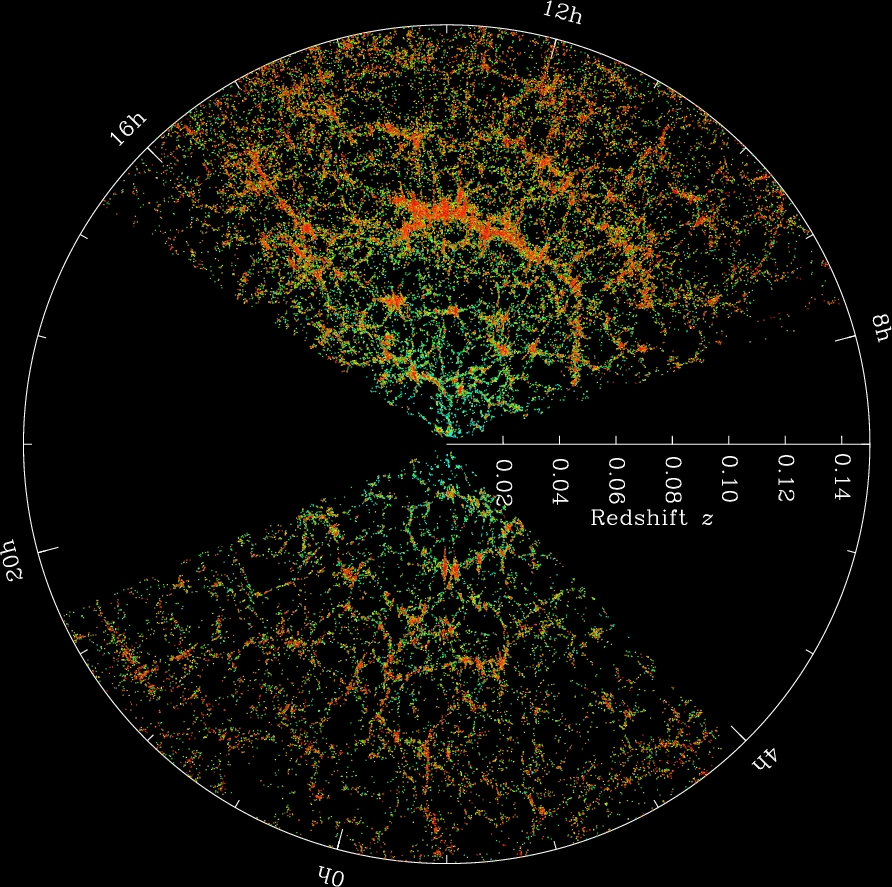
\includegraphics[width=\textwidth]{sdss}
\caption{The cosmic web of the large-scale matter distribution, as traced by galaxies detected by the Sloan Digital Sky Survey (SDSS; \cite{York2000}; \cite{Blanton2017}). Image by M. Blanton and SDSS.}
\label{co_Fig:cosmic_web}
\end{figure}

These anisotropies are believed to arise from quantum fluctuations in the early Universe, which later resulted in over- and underdense regions of matter, which evolved under gravity to give the structures we observe today. This is strongly supported by measurements of baryon acoustic oscillations (which will be described in \autoref{co_Sec:BAO}) and by observations of the cosmic microwave background (CMB), which have revealed that the early Universe was extremely smooth, with small anisotropies of order one part in $10^5$. The CMB and its anisotropies will be described in more detail in \autoref{co_Sec:CMB}.

\subsection{Cosmic expansion and redshift}

After the cosmological principle, perhaps the most fundamental aspect of the standard model of the Universe is that it is expanding. Mathematically, this can be described simply using the scale factor, $a \left( t \right)$, where any distance $d$ at time $t$ is given by
\begin{equation}
d \left( t \right) = a \left( t \right) d_0,
\end{equation}
where $d_0$ is the distance today ($t = t_0$), and the current value of the scale factor, $a_0$, is defined as
\begin{equation}
a_0 = 1.
\end{equation}

For any time in the past, $t < t_0$,
\begin{equation}
a \left( t < t_0 \right) < 1,
\end{equation}
and therefore distances were shorter than they are today. Rewound far enough, this implies that at one stage the Universe was infinitely dense. This is called the Big Bang, and is a central part of the standard cosmological model.

% If distances were shorter in the past, then so too were wavelengths of light and other radiation that was emitted at the time, and has been effectively stretched on its way to the observer.
If distances were shorter in the past, then so too were wavelengths of light and other radiation. The wavelength of any photon has subsequently been stretched between its emission in the past and its observation today.
This effect is called redshift. Since the finite speed of light means that observations of any distant object are equivalent to looking back in time, redshift is a useful measure of the distance of objects from the Earth. Redshift, $z$, can be quantified as
\begin{equation}
1 + z = \frac{\lambda_\text{obs}}{\lambda_\text{emit}}
= \frac{1}{a \left( t \right)},
\end{equation}
where $\lambda_\text{emit}$ and $\lambda_\text{obs}$ are the emitted and observed wavelengths of light.

Evidence for the expanding Universe comes from the Hubble law \citep{Lemaitre1927, Hubble1929}, which states that distant galaxies are receding at a speed $v$ proportional to their distance $d$:
\begin{equation}
v = H_0 d,
\label{co_Eqn:hubble_law}
\end{equation}
where the constant of proportionality is the Hubble constant $H_0$. Despite its name, $H_0$ is today considered as the current value of a time-varying parameter $H \left( t \right)$, which is related to the scale factor $a$ as
\begin{equation}
H = \frac{\dot{a}}{a},
\label{co_Eq:hubble_param}
\end{equation}
where the overdot denotes a time derivative. A more recent diagram of the Hubble law is shown in \autoref{co_Fig:hubble_diagram}. This was compiled from Type Ia supernovae, which will be described in \autoref{co_Sec:supernovae}, and is taken from \citet{Kirshner2004}. Strong evidence for the implied Big Bang is supplied by observations of the CMB (\autoref{co_Sec:CMB}).

\begin{figure}
\centering
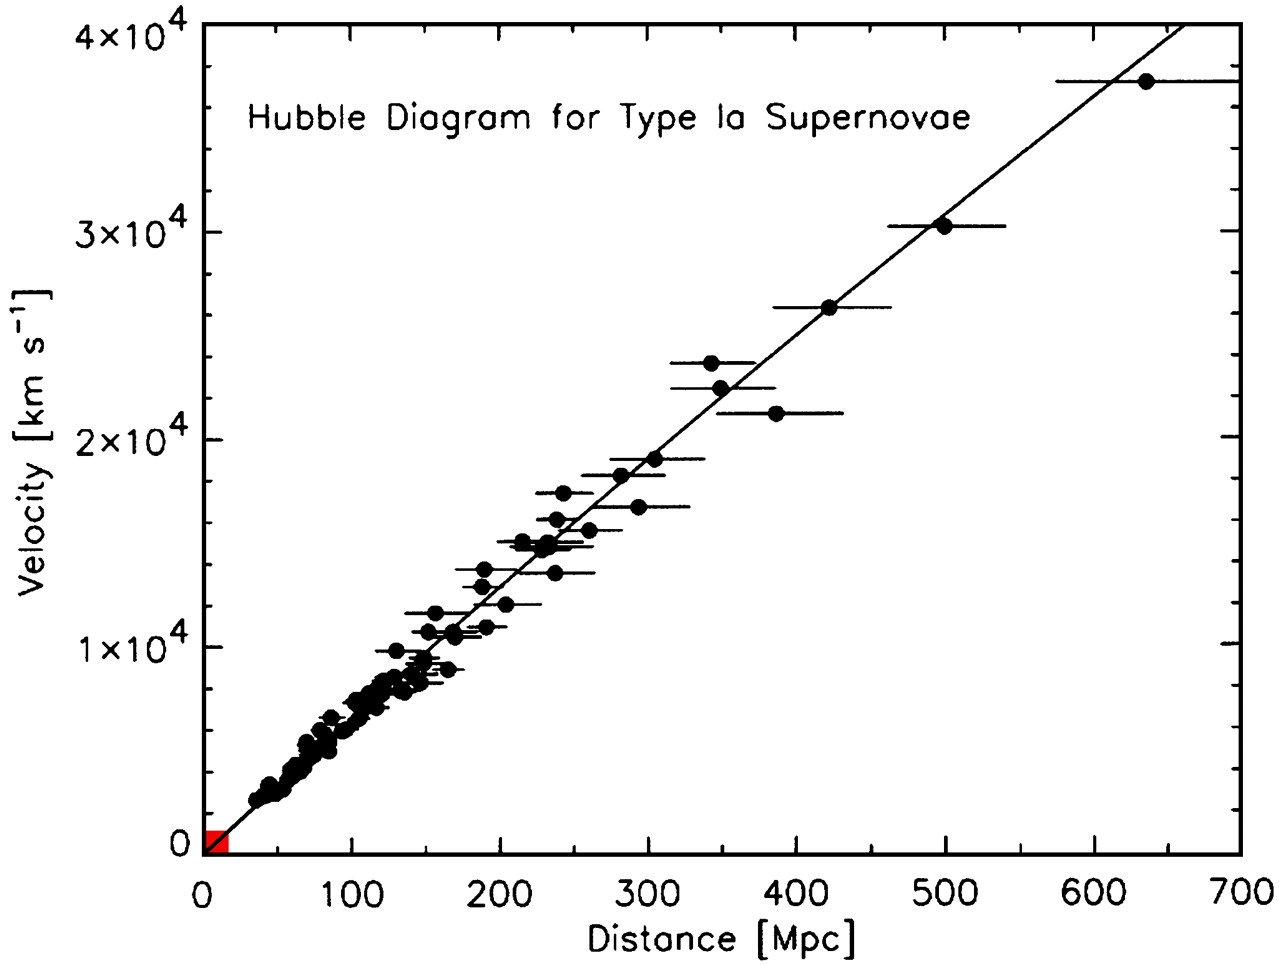
\includegraphics[width=.8\textwidth]{hubble_diagram}
\caption{Diagram of the Hubble law (\autoref{co_Eqn:hubble_law}) relating the recession velocity of distant objects (in this case Type Ia supernovae, which are described in \autoref{co_Sec:supernovae}) to their distance. Taken from \citet{Kirshner2004}.}
\label{co_Fig:hubble_diagram}
\end{figure}

\subsection{The FLRW Universe}

This section provides an overview of some of the mathematics underpinning the standard model of cosmology. It is named after four of its key contributors: Friedmann, Lema\^itre, Robertson and Walker.

In \lcdm{} and simple extensions such as $w$CDM, the Universe is governed by the theory of general relativity (GR), which describes the relationship between the geometry of the Universe and its contents. GR provides a near-universal theory of gravity covering both everyday and cosmological scales (though it notably fails on quantum scales). GR is summarised in the Einstein field equations, which may in fact be written as a single equation \citep{Einstein1916},
\begin{equation}
G_{\mu \nu} + \Lambda g_{\mu \nu}
= \frac{8 \pi G}{c^4} T_{\mu \nu}.
\label{co_Eqn:einstein}
\end{equation}
$G_{\mu \nu}$ in Equation \eqref{co_Eqn:einstein} is the Einstein tensor describing the curvature of spacetime, and $T_{\mu \nu}$ is the energy--momentum tensor describing the energy density at a given point in spacetime. $g_{\mu \nu}$ is the metric tensor, which describes the geometric and causal structure of spacetime, and is related to the separation between points in spacetime, which is discussed below. In Equation \eqref{co_Eqn:einstein} it multiplies the cosmological constant $\Lambda$, which could alternatively be absorbed into $T_{\mu \nu}$, where it could also be replaced with a time-varying dark energy contribution to the density. The Einstein field equations are related to the Newtonian theory of gravity through the classical gravitational constant $G$.

Distances between points in a homogeneous, isotropic and expanding Universe can be quantified using the FLRW metric, which decomposes the line element of spacetime $\text{d}s$ into contributions from time $\text{d}t$ and space, $\text{d}\Sigma$,
\begin{equation}
\text{d}s^2 = - c^2 \text{d}t^2 + a \left( t \right)^2
\text{d}\Sigma^2.
\end{equation}
The spatial metric is further decomposed, in hyperspherical coordinates, into a radial contribution $\text{d}\chi$ and an angular contribution $\text{d}\Omega$ as
\begin{equation}
\text{d}\Sigma^2 = \text{d}\chi^2 + S_K \left( \chi \right)^2
\text{d}\Omega^2.
\label{co_Eqn:spatial_metric}
\end{equation}
$\chi$ is the comoving angular distance, defined in terms of the scale factor $a$ as
\begin{equation}
\chi \left( a \right) = c \int_a^1 {
\frac{ \text{d}a' }{a'^2 H \left( a' \right)}
}.
\end{equation}
The angular line element $\text{d}\Omega$ is given in terms of polar and azimuthal contributions $\text{d}\theta$ and $\text{d}\phi$ as
\begin{equation}
\text{d}\Omega^2 = \text{d}\theta^2
+ \sin^2 \left( \theta \right) \text{d}\phi^2.
\end{equation}
$S_K \left( \chi \right)$ in Equation \eqref{co_Eqn:spatial_metric} is the comoving angular diameter distance, whose value depends on the curvature of the Universe $K$. Specifically, it takes different forms in three cases: a closed Universe with spherical geometry ($K > 0$), a flat Universe with Euclidean geometry ($K = 0$), or an open Universe with hyperbolic geometry ($K < 0$). The comoving angular diameter distance in each of these cases is given by
\begin{equation}
S_K \left( \chi \right) =
\begin{cases}
K^{-\frac{1}{2}} \sin{\left( K^{\frac{1}{2}} \chi \right)}
& \quad \text{for $K > 0$ (closed);} \\
\chi
& \quad \text{for $K = 0$ (flat);} \\
\left| K \right|^{-\frac{1}{2}}
\sinh{\left( \left| K \right|^{\frac{1}{2}} \chi \right)}
& \quad \text{for $K < 0$ (open).} \\
\end{cases}
\label{co_Eqn:angular_diameter_distance}
\end{equation}

The spacetime line element in the FLRW metric, $\text{d}s$, can be related to the metric tensor $g_{\mu \nu}$ from Equation \eqref{co_Eqn:einstein} as
\begin{equation}
\text{d}s^2 = g_{\mu \nu} \text{d}x^\mu \text{d}x^\nu,
\end{equation}
where $\text{d}x^\mu$ is the infinitesimal displacement in comoving coordinates; that is, spacetime coordinates defined such that the spatial component remains constant in the expanding Universe.

It is typical to model the constituents of the Universe as perfect fluids, which are completely described by their energy density $\rho$ and isotropic pressure $P$. Under this assumption, a solution to the Einstein field equations for a homogeneous, isotropic and expanding Universe governed by the FLRW metric is given by the Friedmann equations \citep{Friedmann1922, Friedmann1924},
\begin{equation}
H^2 = \left( \frac{\dot{a}}{a} \right)^2
= \frac{8 \pi G}{3} \rho
+ \frac{\Lambda c^2}{3}
- \frac{K c^2}{a^2};
\label{co_Eq:friedmann}
\end{equation}
\begin{equation}
\frac{\ddot{a}}{a} = - \frac{4 \pi G}{3}
\left( \rho + \frac{3 P}{c^2} \right) + \frac{\Lambda c^2}{3}.
\end{equation}

These two equations can be used to derive a third, the energy conservation equation:
\begin{equation}
\dot{\rho} = - 3 H \left( \rho + \frac{P}{c^2} \right).
\label{co_Eq:energy_conservation}
\end{equation}

Under the assumption that the constituents of the Universe may be modelled as perfect fluids, the equation of state relating the density $\rho_X$ and pressure $P_X$ for a given constituent $X$ is
\begin{equation}
P_X = w_X \rho_X c^2,
\end{equation}
where $w_X$ is the dimensionless equation of state parameter. In this thesis, the symbol $w$ will be used without any subscript to denote the equation of state parameter for dark energy. This parameter is discussed further in \autoref{co_Sec:dark_energy}.

The energy conservation equation (\autoref{co_Eq:energy_conservation}) may be used to derive an expression for the evolution of the density of constituent $X$:
\begin{equation}
\frac{\text{d} \ln{\rho_X}}{\text{d} \ln{a}} + 3 \left( 1 + w_X \right) = 0.
\end{equation}
When $w_X$ is constant, this equation has a solution,
\begin{equation}
\rho_X \propto a^{-3 \left( 1 + w_X \right)}.
\label{co_Eq:rho_dependence_on_a}
\end{equation}

When a given component is dominant, the resulting evolution of the scale factor as a function of time may be found by substituting $\rho_X$ into Equation \eqref{co_Eq:friedmann}. Values of $w_X$ for the different constituents of the Universe and the resulting evolution of the scale factor will be discussed in \autoref{co_Sec:expansion_history}.

\subsection{Constituents of the Universe}
\label{co_Sec:constituents}

\subsubsection{Baryonic matter}

Baryonic matter is the ordinary matter that makes up what we see on Earth and within the solar system. The term is commonly used to include not only baryons---particles composed of three quarks, including protons, neutrons, and their higher-energy counterparts---but more generally any form of matter as described by the standard model of particle physics. Today it constitutes around 4.9\% of the total energy density of the Universe \citep{Planck2018VI}. Compared to dark matter and dark energy, baryonic matter is much better understood. Countless high-precision tests of the standard model have been carried out at particle colliders and elsewhere, with no significant deviations from the theoretical predictions yet detected \citep[e.g.][for a review]{Erler2019}.

However, there are many contradictions between the predictions of the standard model and observations of the Universe. For example, in addition to its failure to describe dark matter and dark energy (and gravity), it predicts that there should be an equal amount of matter and antimatter, which is not observed. Discrepancies such as these continue to motivate a large amount of active research in particle physics.

\subsubsection{Dark matter}

Several independent forms of observational evidence point towards the existence of some additional form of matter, constituting around 25.9\% of the energy density of the Universe \citep{Planck2018VI}. This has come to be known as dark matter, since it does not interact electromagnetically and cannot be `seen' directly in the traditional sense. It has only been observed to interact gravitationally, although many theories predict some small amount of interaction by other means, such as via the weak interaction.

The first evidence for dark matter arrived in the form of an excess in the observed orbital velocities of stars in nearby galaxies \citep{Kapteyn1922}, and then galaxies themselves in clusters \citep{Zwicky1933,Zwicky1937}, compared to the velocities that could be explained by the amount of visible matter. Without an alternative theory of gravity, these observed galaxy rotation curves could only be explained by an invisible form of matter---roughly five times as much as the visible, baryonic matter. An example of a galaxy rotation curve is shown in \autoref{co_Fig:rotation}. The data points can only be explained by combining the visible `disk' component with an invisible dark matter `halo'.

\begin{figure}
\centering
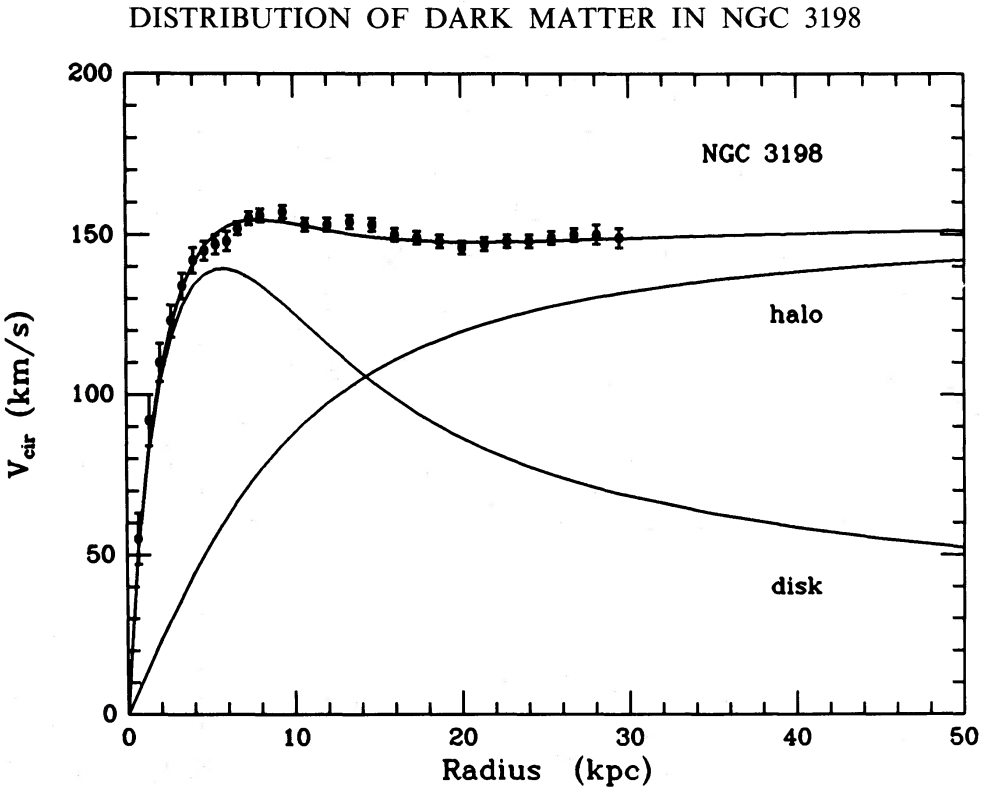
\includegraphics[width=.8\textwidth]{rotation}
\caption{A galaxy rotation curve taken from \citet{vanAlbada1985}. The data points can only be explained by combining the visible `disk' component with an invisible dark matter `halo'.}
\label{co_Fig:rotation}
\end{figure}

More direct evidence for dark matter has been provided by weak lensing mass reconstructions of galaxy cluster collisions, such as those of the Bullet Cluster. The reconstructed matter distribution of this cluster was revealed to extend far beyond its visible limits, and furthermore is inconsistent with a simple modification of gravity at a significance of $8\sigma$ \citep{Clowe2004, Clowe2006}. The observations of the Bullet Cluster also demonstrate the collisionless nature of dark matter \citep{Markevitch2004}.

Further evidence for the existence of dark matter comes from observations of the CMB. Around six times the amount of matter that we observe directly is needed to achieve a good fit to the \lcdm{} model \citep{Planck2018VI}. The CMB will be discussed further in \autoref{co_Sec:CMB}.

Dark matter is required to be `cold', i.e. sufficiently massive as to move non-relativistically, in order to explain the observed level of structure in the present-day Universe \citep{Bond1982, Blumenthal1982, Peebles1982, Blumenthal1984, Davis1985}.

However, despite the relative abundance of observational evidence for dark matter, a direct detection on Earth continues to be elusive. Collider experiments have performed extensive searches over the past decade, and classes of physical models of dark matter that were not long ago believed to be likely have now been largely ruled out \citep{Trevisani2018, Aaboud2018, ATLAS2019}.

\subsubsection{Dark energy}
\label{co_Sec:dark_energy}

Almost all of the remaining energy density in the Universe---around 69.1\% \citep{Planck2018VI}---is believed to be some additional unknown form of energy responsible for the accelerating expansion of the Universe. This additional form of energy is known as dark energy.

\subsubsubsection{Evidence for dark energy}

The main evidence for the existence of dark energy comes from the accelerating expansion of the Universe, which was discovered by precision observations of distant Type Ia supernovae in the late 1990s \citep{Riess1998, Perlmutter1999}. Type Ia supernovae will be discussed further in \autoref{co_Sec:supernovae}. This accelerating expansion cannot be explained under GR without a large additional and previously unknown contribution to the total energy density.

Measurements of CMB anisotropies indicate that the Universe is flat or almost flat \citep{Planck2018VI}. Under the \lcdm{} model, this cannot be explained by matter alone, including dark matter, and therefore requires a large contribution from dark energy. Probes of the large scale structure of the Universe, such as weak lensing, also detect too little matter for flatness \citep[e.g.][]{DES2021}.

\subsubsubsection{Models of dark energy}

\paragraph{Cosmological constant}

The mathematically simplest way to account for an additional energy source in GR and its solutions is with a cosmological constant, $\Lambda$. The cosmological constant was first introduced by Einstein in his original descriptions of GR \citep{Einstein1917} in order to provide a steady state Universe, which was generally assumed to be the case at the time, when his equations otherwise predicted a dynamic Universe. After the Universe was discovered to in fact be expanding, the cosmological constant was assumed to be zero, and Einstein is alleged to have described its initial inclusion as his ``biggest blunder'' \citep{ORaifeartaigh2018}. However, after the accelerating expansion was discovered, the cosmological constant was reinstated and today forms an essential pillar of the \lcdm{} standard model of cosmology.

The cosmological constant gives a dark energy equation of state parameter $w$ of
\begin{equation}
w = -1.
\end{equation}

Physically a cosmological constant corresponds to an intrinsic vacuum energy of space. Such a vacuum energy is predicted by the standard model of particle physics, but is around 120 orders of magnitude too large to explain cosmological observations \citep[e.g.][]{Adler1995}. This is known as the cosmological constant problem, and is one of the major outstanding questions in fundamental physics.

\paragraph{Quintessence}

The term quintessence refers to a proposed new scalar field, many plausible models of which exist (see \citealt{Tsujikawa2013} for a review). Such a field could change over time, such that the dark energy equation of state parameter $w$ is a function of the scale factor $a$,
\begin{equation}
w = w \left( a \right).
\label{co_Eq:quintessence}
\end{equation}

It is common to Taylor expand Equation \eqref{co_Eq:quintessence} to linear order about $a = 1$ to define $\wo$ and $\wa$ as
\begin{equation}
w \left( a \right) = w_0 + w_a \left( 1 - a \right),
\label{co_Eq:w_a_taylor}
\end{equation}
such that
\begin{align}
w_0 &= w \left( a = 1 \right);
\\
w_a &= - \frac{\text{d}w}{\text{d}a} \left( a = 1 \right).
\label{co_Eq:wa}
\end{align}

Observations to date are consistent with the values of
\begin{align}
w_0 &= -1; \\
w_a &= 0
\end{align}
(e.g. \cite{Ribeiro2019}, from a combined analysis of CMB anisotropies, baryon acoustic oscillations, supernovae and cosmic chronometers), which corresponds to a cosmological constant.

\paragraph{Modified gravity}

It is possible to negate the need for dark energy altogether with suitable modifications to gravity, which deviate from GR \citep[e.g.][]{Nojiri2003, Nojiri2011, Nicolis2009, Clifton2012, Nojiri2017}. Alternatively, dark energy could exist alongside a modified theory of gravity. However, all observations to date are consistent with GR, provided that dark energy is included, and some modified gravity models have been ruled out by recent observations of gravitational waves \citep{Blas2016, Vainio2017, Arai2018, Battye2018, Ma2019}. Pulsar timing experiments also place tight constraints on deviations from GR \citep{BeltranJimenez2016, Shao2017, Cai2019, Kramer2021}.

\subsubsection{Other constituents}

The Universe also contains small amounts of `radiation', totalling less than 1\% of the total energy density. This includes neutrinos, and the CMB, which will be described further in \autoref{co_Sec:CMB}.

\subsection{Expansion history}
\label{co_Sec:expansion_history}

The Universe today is dominated by dark energy, but this is a fairly recent development. Prior to this, the Universe is believed to have gone through several epochs in which different components were dominant, each of which will now be described.

\subsubsection{Inflation}

It is believed that the early Universe underwent a short period of rapid expansion, known as inflation \citep{Guth1981, Guth1982, Starobinsky1982,  Linde1982, Linde1983}. The inflationary period is thought to have lasted from $10^{-36}$\,s to $10^{-33}$--$10^{-32}$\,s after the Big Bang, during which the Universe expanded by around 60 $e$-folds (a factor of $10^{26}$) \citep{Planck2018X}. Inflation provides a mechanism to create the seeds for the present-day large-scale structure of the Universe, by vastly magnifying quantum fluctuations in the early Universe. The popularity of the theory is also driven by its ability to solve two significant cosmological problems: the horizon problem and the flatness problem.

The horizon problem is the fact that the CMB is isotropic to within one part in $10^5$, implying that regions far apart on the sky must have been in thermal equilibrium in the early Universe, when---in the absence of inflation---they could have never been in causal contact. Invoking inflation allows seemingly distant parts of the CMB sky to have been in causal contact prior to inflationary expansion.

The flatness problem arises from the observation that the present-day Universe is extremely close to flat \citep{Planck2018VI}. It can be shown from Equations \eqref{co_Eq:friedmann}--\eqref{co_Eq:energy_conservation} that flatness is an unstable equilibrium, in that any perturbation from flatness should grow over time. Therefore, the fact that the Universe is extremely close to flat today implies that any deviation from flatness in the early Universe must have been infinitesimal---of order $10^{-55}$ or smaller \citep{Guth1981}. The lack of an explanation---in the absence of inflation---for this suspiciously convenient value is a type of `fine-tuning' problem. Inflation provides an explanation, because such a rapid expansion of the Universe strongly suppresses any previous cosmic curvature and leaves a Universe sufficiently flat to explain current observations.

Inflation is also able to predict the observed value of the scalar spectral index $n_s$ \citep{Bardeen1983, Planck2018X}. (The scalar spectral index and other parameters of the \lcdm{} model are discussed in \autoref{co_Sec:free_params}.) Physically, inflation can be explained by a new scalar `inflaton' field, many plausible models of which exist \citep[e.g.][for a review]{Bauman2015}. Future CMB polarisation experiments hope to detect direct evidence of the inflaton field, which would confirm the theory of inflation and constrain physical models (see \autoref{co_Sec:CMB}).

\subsubsection{Radiation domination}

The Universe subsequently underwent a period of radiation domination, during which the dominant components were relativistic photons and neutrinos. Radiation is modelled as a gas, exerting a positive pressure in each of three spatial dimensions, giving it an equation of state parameter $w_\text{r}$ of
\begin{equation}
w_\text{r} = \frac{1}{3}.
\end{equation}
Inserting this into Equation \eqref{co_Eq:rho_dependence_on_a} gives the evolution of the radiation density $\rho_\text{r}$ as
\begin{equation}
\rho_\text{r} \propto a^{-4}.
\label{co_Eq:radiation_density_evolution}
\end{equation}
When radiation is dominant, the first Friedmann equation (\autoref{co_Eq:friedmann}) then becomes
\begin{equation}
H^2 \propto a^{-4}.
\end{equation}
Using the definition of the Hubble parameter $H$ in terms of the time derivative of the scale factor (\autoref{co_Eq:hubble_param}), we can obtain a solution for the scale factor as a function of time in the epoch of radiation domination,
\begin{equation}
a \propto t^{1/2}.
\end{equation}

\subsubsection{Matter domination}

The period of radiation domination was followed by a period of matter domination. Matter is pressureless, and therefore its equation of state parameter $w_\text{m}$ is
\begin{equation}
w_\text{m} = 0,
\end{equation}
giving the evolution of the matter density $\rho_\text{m}$ as
\begin{equation}
\rho_\text{m} \propto a^{-3}.
\end{equation}
Comparing this to Equation \eqref{co_Eq:radiation_density_evolution} for radiation explains why matter eventually came to dominate over radiation, since radiation was more heavily diluted by the expansion of the Universe. This effect can be understood in terms of redshift: as the Universe expanded, radiation is redshifted, decreasing its energy by an additional factor $1/a$.

In the epoch of matter domination, the Hubble parameter evolves as
\begin{equation}
H^2 \propto a^{-3},
\end{equation}
which gives the evolution of the scale factor as
\begin{equation}
a \propto t^{2/3}.
\end{equation}
Despite the faster growth of the scale factor during matter domination, it was in this period that structure was most able to form. Structure formation was strongly suppressed in the period of radiation domination by the high density of relativistic particles.

\subsubsection{Dark energy domination}
\label{co_Sec:de_domination}

The Universe is now in a period of dark energy domination. The dark energy equation of state parameter $w$ is either exactly or approximately equal to $-1$, depending on the model (see \autoref{co_Sec:dark_energy}). Inserting a value of $w = -1$, corresponding to a cosmological constant $\Lambda$, into Equation \eqref{co_Eq:rho_dependence_on_a} gives
\begin{equation}
\rho_\Lambda \propto 1,
\end{equation}
i.e. a constant density. This is how dark energy has come to eventually dominate, as the density of matter and radiation is diluted by the expanding Universe. For dark energy domination, Equation \eqref{co_Eq:friedmann} gives that
\begin{equation}
H^2 = \frac{\Lambda c^2}{3},
\end{equation}
which has an exponential solution for the scale factor:
\begin{equation}
a \propto \exp{\left[ \sqrt{\frac{\Lambda}{3}} c t \right]}.
\end{equation}
Under dark energy domination, therefore, the Universe undergoes exponential growth,\linebreak which suppresses structure formation. This means that the growth of structure as a function of redshift $z$ (or equivalently, the scale factor $a$) depends heavily on the nature of dark energy and its potential time evolution. Observational probes of structure growth and the recent expansion history of the Universe are therefore able to potentially place tight constraints on dark energy models via their predictions of $w \left( a \right)$.

\subsection{Density parameters}

It is convenient to define the critical density $\rho_\text{c}$, as the density required for a flat Universe, obtained by setting $K = 0$ and $\Lambda = 0$ in Equation \eqref{co_Eq:friedmann}:
\begin{equation}
\rho_\text{c} = \frac{3 H^2}{8 \pi G}.
\end{equation}
For each component $X$ of the Universe, we may then define the density parameter $\Omega_\text{x}$,
\begin{equation}
\Omega_\text{x} = \frac{\rho_\text{x}}{\rho_\text{c}}.
\end{equation}
We may include the curvature contribution to the Friedmann equation in this form too by defining it as a density $\rho_K$,
\begin{equation}
\rho_K = -\frac{3 K c^2}{8 \pi G a^2},
\end{equation}
giving the curvature density parameter $\Omega_K$,
\begin{equation}
\Omega_K = \frac{\rho_K}{\rho_\text{c}}
= -\frac{K c^2}{a^2 H^2}.
\end{equation}
Including a general dark energy contribution, the Friedmann equation (\autoref{co_Eq:friedmann}) may then be written in form which makes explicit the way in which the different components evolve over time:
\begin{equation}
\frac{H^2}{H_0^2} =
\frac{\Omega_\text{r}}{a^4} +
\frac{\Omega_\text{m}}{a^3} +
\frac{\Omega_K}{a^2} +
\frac{\Omega_\text{DE}}{a^{3 \left( 1 + w \right)}}.
\label{co_Eq:freidmann_as_omegas}
\end{equation}
If dark energy is a cosmological constant, then the last term in Equation \eqref{co_Eq:freidmann_as_omegas} becomes simply $\Omega_\Lambda$, with
\begin{equation}
\Omega_\Lambda = \frac{\Lambda c^2}{3 H^2}.
\end{equation}

\subsection{Free parameters}
\label{co_Sec:free_params}

The minimal \lcdm{} model has six free parameters. There is not a single unique parameterisation, but a typical choice is the following \citep[e.g.][]{DiValentino2015}:

\begin{itemize}
\item The Hubble parameter $H_0$, which may alternatively be described using the dimensionless Hubble parameter $h$,
\begin{equation}
h = \frac{H_0}{100\,\text{km}\,\text{s}^{-1}\,\text{Mpc}^{-1}}.
\label{co_Eq:h_definition}
\end{equation}
\item $\omb h^2$, where $\omb$ is the energy density of baryons as a fraction of the critical density.
\item $\omc h^2$, where $\omc$ is the dark matter energy density as a fraction of the critical density.
\item The amplitude of primordial scalar perturbations $A_s$.
\item The scalar spectral index $n_s$, describing the scale dependence of primordial perturbations.
\item The optical depth to reionisation $\tau$: a physical description of the redshift of the epoch of reionisation, which was a period in the evolution of the Universe when the first stars and other luminous sources were formed, and were able to ionise hydrogen in the intergalactic medium.
\end{itemize}

Other parameters may be derived from these six, and vice versa. The parameters that are constrained by a particular experiment will depend on the cosmological probe in question. Two derived parameters that are of interest in this thesis are:
\begin{itemize}
\item $\omm$, the total matter density, given by
\begin{equation}
\omm = \omc + \omb.
\end{equation}
\item $\sie$, the amplitude of present-day matter fluctuations on scales of $8\,h^{-1}\,\text{Mpc}$. This may be constrained directly by probes of large scale structure, but can also be predicted by the \lcdm{} model given the free parameters listed above.
\end{itemize}

The \lcdm{} model may be extended by adding additional parameters. One extension is of particular interest in this thesis, which is the extension to time-varying dark energy via a dark energy equation of state parameter that depends on the scale factor as $w \left( a \right)$. As introduced in Equations \eqref{co_Eq:w_a_taylor}--\eqref{co_Eq:wa}, this may be Taylor expanded to linear order to define $w_0$ and $w_a$, which are the two cosmological parameters of greatest interest to this thesis. The extension to \lcdm{} to include $w_0$ and $w_a$ is often called \wcdm{}.

Current constraints on the ten parameters listed above are given in \autoref{co_Tbl:params}. These are taken from \citet{Planck2018VI}, where they are derived from CMB temperature, polarisation and lensing, combined with baryon acoustic oscillations and, for the dark energy parameters $w_0$ and $w_a$, Type Ia supernovae. Each of these probes is described in \autoref{co_Sec:obs_probes}.

\begin{table}
\caption{Current constraints on the ten cosmological parameters described in \autoref{co_Sec:free_params}. Taken from \citet{Planck2018VI} Tables 2 and 6, where they are derived from CMB temperature, polarisation and lensing, combined with baryon acoustic oscillations and, for $w_0$ and $w_a$, Type Ia supernovae.}
\label{co_Tbl:params}
\vspace{.5em} % for some reason I couldn't find a way to automate this
\centering
\bgroup
\def\arraystretch{1.5}
\begin{tabular}{ll}
% \hline
Parameter & Best-fit value $\pm$ 68\% limits \\
\hline
$H_0 \left[ \text{km}\,\text{s}^{-1}\,\text{Mpc}^{-1} \right]$
& $67.66 \pm 0.42$ \\
$\omb h^2$ & $0.02242 \pm 0.00014$ \\
$\omc h^2$ & $0.11933 \pm 0.00091$ \\
$10^9 A_s$ & $2.105 \pm 0.030$  \\
$n_s$ & $0.9665 \pm 0.0038$ \\
$\tau$ & $0.0561 \pm 0.0071$ \\
\hline
$\omm$ & $0.3111 \pm 0.0056$ \\
$\sie$ & $0.8102 \pm 0.0060$ \\
\hline
$\wo$ & $-0.957 \pm 0.080$ \\
$\wa$ & $-0.29\substack{+0.32 \\ -0.26}$
\end{tabular}
\egroup
\end{table}

\section{Outstanding questions}
\label{co_Sec:open_questions}

The previous section has described in some detail the current best understanding of the nature of the Universe. However, many questions remain outstanding. Below is a brief summary of a selection of key open questions in cosmology.

\begin{itemize}
\item \textbf{Nature of the constituents.} As described in \autoref{co_Sec:constituents}, around 95\% of the energy density of the Universe consists of dark energy and dark matter. However, the physical nature of both of these components remains unknown, along with an explanation for why the cosmological constant does not correspond to the vacuum energy predicted by the standard model of particle physics.
\item \textbf{Modified gravity.} Is GR correct, or is a modified theory of gravity required?
\item \textbf{Inflation.} What is the physical nature of the mechanism responsible for inflation?
\item \textbf{Tensions in measured parameters.} It is common for different experiments to infer values of cosmological parameters that are not in perfect agreement. However, two particular discrepancies have arisen between experiments measuring the late-time Universe and the early Universe. The most significant of these is the tension in the Hubble parameter $H_0$, between local measurements of Type Ia supernovae calibrated by Cepheid variable stars using the distance ladder method (which will be described in \autoref{co_Sec:supernovae}), and values inferred from CMB observations conditioned on the \lcdm{} model. This tension between early and late time measurements is illustrated in \autoref{co_Fig:h0_tension}. This figure is taken from \citet{DiValentino2021Hubble}, since which the tension has been claimed to have reached the $5 \sigma$ significance level \citep{Riess2021b}. The second tension of interest is in the parameter $S_8$, defined as\footnote{The power of $0.5$ in Equation \eqref{co_Eqn:s8} is sometimes varied slightly depending on the best fit to the data, such as to $0.48$ in \citet{Rhodes2001}.}
\begin{equation}
S_8 = \sigma_8 \left[ \frac{\omm}{0.3} \right]^{0.5},
\label{co_Eqn:s8}
\end{equation}
between local measurements using weak lensing compared to those inferred from CMB observations. This tension is currently claimed to stand at the 2--3$\sigma$ level based on one recent weak lensing analysis from the Kilo-Degree Survey \citep{Heymans2021}, although better agreement with the CMB is found by the Dark Energy Survey \citep{DES2021}. (Both of these current weak lensing surveys will be described in \autoref{co_Sec:observational_history}.) While the $S_8$ tension may just be a statistical fluke, or the result of undiagnosed systematic errors, the $H_0$ tension has persisted and strengthened despite being repeatedly examined with increasing care \citep[e.g.][]{Riess2018b, Riess2018c, Riess2018a, Riess2020, Riess2021a, Riess2021b, Burns2018, Yuan2019, Reid2019, Macaulay2019, Soltis2021, Anand2021, Romaniello2021}, and a resolution may require new physics \citep{DiValentino2021Hubble}.
\end{itemize}

\begin{figure}
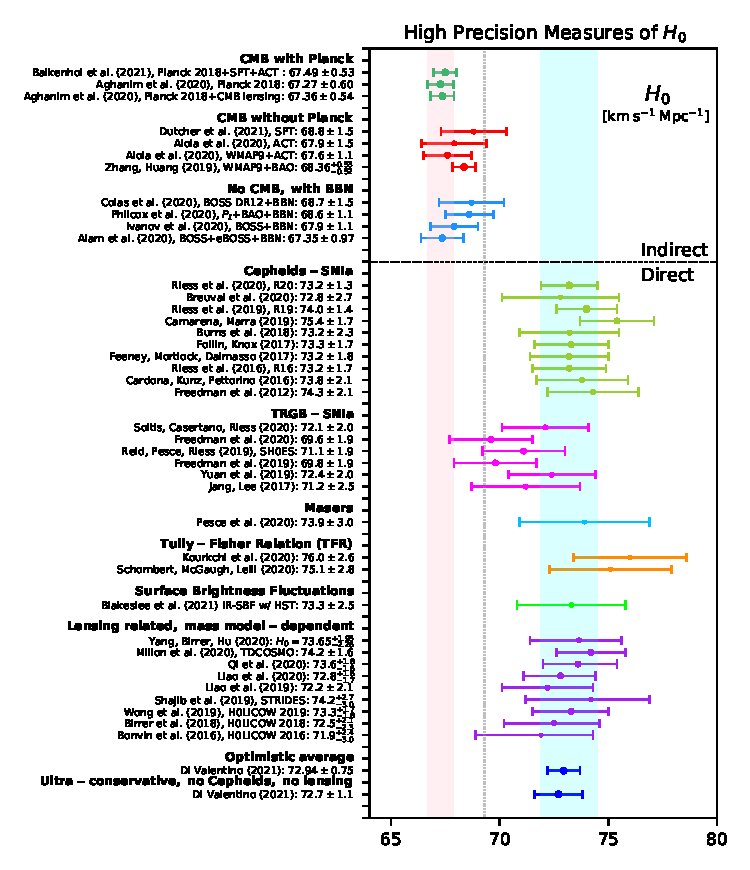
\includegraphics[width=\textwidth]{h0_tension}
\caption{Tension in measurements of the Hubble parameter $H_0$ between early (indirect) and late time (direct) observations. Figure taken from \citet{DiValentino2021Hubble}. Error bars are 68\% credible intervals. The blue band corresponds to the result from \citet{Riess2020} and the pink to those from \citet{Planck2018VI}.}
\label{co_Fig:h0_tension}
\end{figure}

\section{Observational probes}
\label{co_Sec:obs_probes}

There are a number of observational methods by which our current best understanding of the Universe, as described in \autoref{co_Sec:std_model}, has been developed, and using which we hope to answer some of the remaining outstanding questions such as those summarised in \autoref{co_Sec:open_questions}. A selection of these methods are described in this section.

\subsection{Cosmic microwave background}
\label{co_Sec:CMB}

\begin{figure}
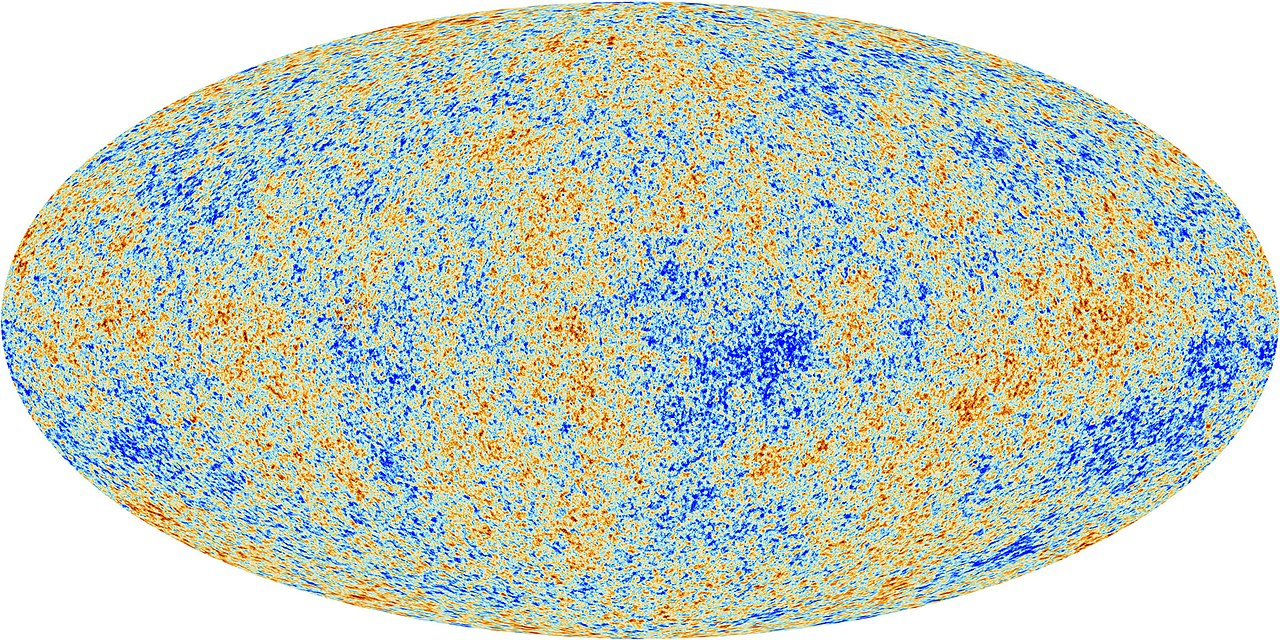
\includegraphics[width=\textwidth]{planck_t}
\caption{Map of CMB temperature anisotropies measured by the \Planck{} satellite \citep{Planck2018I}. Red colours are warmer than average and blue colours cooler, both by up to $300\,\mu\text{K}$.}
\label{co_Fig:planck_t}
\end{figure}

Observations of the cosmic microwave background (CMB) have perhaps offered more insight into the nature of the Universe than any other method. The CMB consists of photons from the early Universe that have been redshifted over time and now reside in the microwave regime, corresponding to a temperature of around 2.7\,K.

The origin of the CMB can be traced back to the first $\sim$\,380\,000 years after the Big Bang, during which the Universe was sufficiently hot that it was impossible for atoms to form without being ionised, and high-energy photons existed in thermal equilibrium with protons and electrons. As the Universe expanded, it cooled, and eventually the photons had insufficient energy to ionise atoms, and the first hydrogen atoms were born. This period, called recombination, occurred at a redshift of $z \sim 1100$.

The CMB contains small anisotropies in both its temperature and polarisation, of order one part in $10^5$ and $10^6$ respectively, which are understood to be the precursor to the large-scale structure in the present-day Universe. (Baryon acoustic oscillations, discussed in \autoref{co_Sec:BAO} below, provide strong evidence for this link between the early and late time Universe.) The scale dependence of these anisotropies, captured by the power spectrum (see \autoref{chap:est_like}), are predicted by the \lcdm{} model and depend closely on its free parameters. As a result, observations of the CMB are able to constrain many cosmological parameters, such as the amount of baryonic matter, dark matter, dark energy and curvature in the Universe, as well as its age and properties of primordial perturbations.

The CMB was proposed and discovered---initially by accident---in the mid-20th century \citep{Gamow1948a, Gamow1948b, Alpher1948a, Alpher1948b, Doroshkevich1964, Penzias1965, Dicke1965}. A series of satellite missions in the late 20th and early 21st centuries made increasingly precise observations, free from interference from terrestrial radio sources. The first was the NASA Cosmic Background Explorer (COBE) mission, which operated from 1989 to 1993 and confirmed that the CMB radiation has an almost perfect blackbody spectrum, consistent with theoretical predictions \citep{Fixsen1996}. It was also able to measure the intrinsic anisotropies for the first time \citep{Bennett1996}. The anisotropies were measured to much higher precision with the subsequent NASA Wilkinson Microwave Anisotropy Probe (WMAP) mission, which operated from 2001 to 2010 and was able to resolve smaller scale features in the CMB temperature power spectrum. Finally, the ESA \Planck{} mission, which operated from 2009 to 2013, achieved higher resolution still, as well as measuring anisotropies in the polarisation of the CMB. The map of CMB temperature anisotropies from the \Planck{} mission is shown in \autoref{co_Fig:planck_t}. The final cosmological analysis of \Planck{} data in \citet{Planck2018VI} stands as the current pinnacle of precision cosmology, achieving sub-percent precision in many cosmological parameters.

Current and future CMB experiments such as the South Pole Telescope \citep{Carlstrom2011}, the Atacama Cosmology Telescope \citep{Swetz2011}, the POLARBEAR experiment \citep{Kermish2012}, the Simons Observatory \citep{so2019}, CMB-S4 \citep{Abazajian2016} and LiteBIRD \citep{Hazumi2019} have science goals including the detection of direct evidence of inflation via the measurement of primordial $B$-mode polarisation \citep{Kamionkowski2016} and the measurement of spectral distortions, which probe the thermal history of the Universe \citep{Chluba2019, Chluba2021}.

\subsection{Gravitational lensing}
\label{co_Sec:gravitational_lensing}

Gravitational lensing is the name given to the distortion of light by gravity. It was predicted by GR \citep{Einstein1916, Einstein1936}, in which gravity is modelled as a consequence of the distortion of spacetime by an uneven distribution of mass,
% which has the effect of bending the path of light as well as massive objects.
which has the effect of not only bending the paths of massive objects but also of light.
The prediction was confirmed soon afterwards, with measurements of the deflection of the images of stars by the gravity of the Sun during a solar eclipse \citep{Dyson1917, Dyson1920}.

\begin{figure}
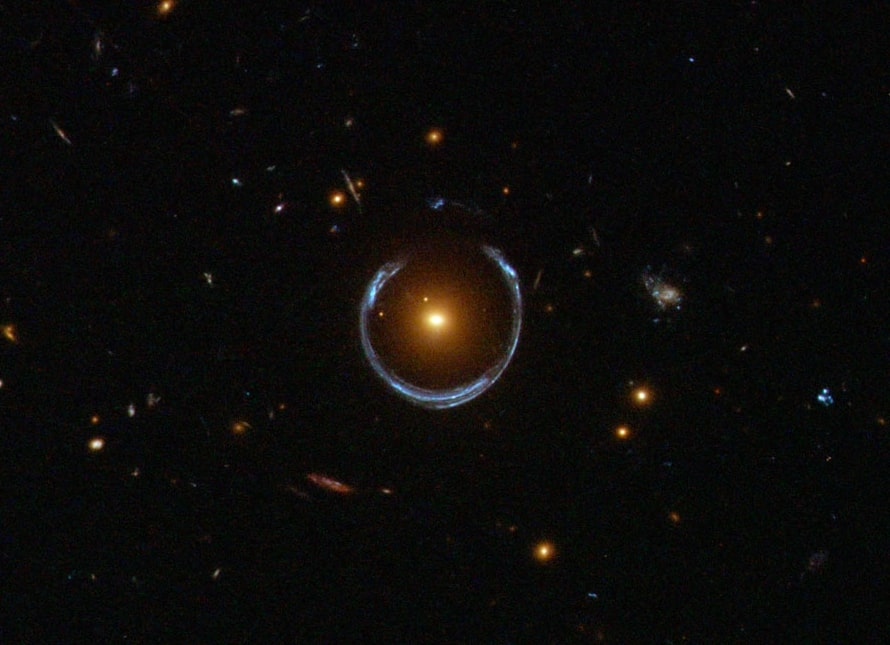
\includegraphics[width=\textwidth]{strong_lens}
\caption{A strong lensing event captured by the Hubble Space Telescope, in which a distant blue galaxy is lensed by a foreground red galaxy. Image credit: ESA/Hubble \& NASA.}
\label{co_Fig:strong_lens}
\end{figure}

Occasionally the alignment of a source and lens object is such that strong lensing occurs, in which the image of the source is distorted so strongly that the lensing effect is obvious without the need for any statistical analysis. An example is shown in \autoref{co_Fig:strong_lens}, in which the image of a distant blue galaxy has been strongly lensed by a foreground red galaxy. Analysis of strong lensing events like this can help to constrain models of dark matter and gravity, since the precise distortion of the source image depends sensitively on these factors \citep[e.g.][]{Vegetti2014, Li2016, Hezaveh2016, Gilman2020, Andrade2022}. Strong lensing observations have also been used to constrain the Hubble parameter $H_0$, because strong gravitational fields not only distort images but also the time taken for light to pass through the field \citep[e.g.][]{Bonvin2017}.

Strong lensing is rare, but essentially every line of sight on the sky is lensed weakly to some degree. This means that observations of distant galaxies are able to trace the large scale structure of the Universe through weak lensing. Weak gravitational lensing is the main observational probe of cosmology considered in this thesis, and is described in more detail in \autoref{co_Sec:weak_lensing}.

\subsection{Type Ia supernovae}
\label{co_Sec:supernovae}

Type Ia supernovae are the end-life stage of binary star systems in which one or both stars is a white dwarf. Accretion onto the white dwarf from its companion eventually takes it beyond a certain threshold mass, which triggers runaway nuclear fusion leading to a supernova explosion.

The usefulness of Type Ia supernovae to cosmology lies in the fact that this fixed critical mass---around 1.44 solar masses---leads to all Type Ia supernovae exploding at the same peak brightness. Such an object of known brightness is known as a standard candle, and allows the calculation of the distance to the object by comparison with the apparent brightness from Earth. Although Type Ia supernovae are thought to all have the same intrinsic peak brightness, this brightness is not itself predicted by theory. This necessitates the calibration of the brightness using observations of supernovae whose distance is known by some other means. A common method involves observations of Cepheid variables in the same galaxies as the supernovae. Cepheid variables are pulsating stars, whose pulsation period is related to their brightness, such that the same method can be used to determine their distance by measuring their pulsation period. The relationship between period and brightness has to itself be calibrated, using parallax measurements of nearby Cepheids. This method of repeated calibration to obtain reliable distance measurements is known as the cosmic distance ladder.

Observations of distant Type Ia supernovae were used to detect cosmic acceleration \citep{Riess1998, Perlmutter1999}, and are still regularly used for determining the Hubble constant $H_0$ \citep{Dhawan2018, Burns2018, Macaulay2019, Taubenberger2019, Khetan2021, Riess2021a, Riess2021b}.

\subsection{Baryon acoustic oscillations}
\label{co_Sec:BAO}

Baryon acoustic oscillations are a particular scale dependence in the large-scale matter distribution in the present-day Universe. They arise from acoustic waves in the early Universe prior to recombination, which were formed from the counteracting forces of gravity and radiation pressure surrounding overdense regions of the primordial plasma. In this period, baryons and photons were coupled, but following recombination the photons free-streamed away to form the CMB, relieving the radiation pressure and leaving the baryons essentially frozen in shells of a particular size. This size is given by the sound horizon at the time of recombination, which can be predicted by theory and has been confirmed to high precision by CMB observations \citep{Planck2018I}. These shells evolved gravitationally to form a distinct signal in the late-time matter distribution in the Universe. Measurements of the baryon acoustic oscillation signal in large-scale structure provide a clear link between scales in the early and late Universe, while measurements of the signal as a function of redshift directly probe the expansion history of the Universe. This defined scale is known as a standard ruler, by analogy with standard candles such as Type Ia supernovae described in \autoref{co_Sec:supernovae} above.

Baryon acoustic oscillations have been detected in the past two decades by galaxy surveys including the Sloan Digital Sky Survey (SDSS; \citealt{Eisenstein2005, Percival2010}), the 2dF Galaxy Redshift Survey (2dFGRS; \citealt{Cole2005}), the 6dF Galaxy Survey (6dFGS; \citealt{Beutler2011}), the WiggleZ Dark Energy Survey \citep{Blake2011, Kazin2014} and the SDSS (extended) Baryon Oscillation Spectroscopic Survey (BOSS/eBOSS; \citealt{Anderson2012, Anderson2014, Delubac2015, deSainteAgathe2019, Blomqvist2019}).

\subsection{Redshift-space distortions}

Redshift-space distortions are distortions of galaxy positions in redshift space relative to their positions in real space, due to additional contributions to their redshift beyond the dominant Hubble expansion. These can be due to orbital Doppler shifts, or general relativistic gravitational redshift. Observations of redshift-space distortions can be used to constrain models of cosmological structure formation \citep{Percival2009, Macaulay2013, Howlett2015} as well as testing GR and constraining theories of modified gravity \citep{Beutler2014, Percival2011, Raccanelli2013}.

\subsection{Gravitational waves}

Gravitational waves are travelling distortions of spacetime emanating from accelerating masses. They are predicted by GR \citep{Einstein1916, Einstein1918} but were only recently directly detected for the first time, by the Laser Interferometer Gravitational-Wave Observatory (LIGO) and the Virgo Interferometer \citep{Abramovici1992, Accadia2012, Abbott2016}. Gravitational wave detections are useful as a test of GR, and have already imposed significant constraints on modified gravity models \citep{Blas2016, Vainio2017, Arai2018, Battye2018, Ma2019}. Gravitational waves resulting from black hole or neutron star mergers may be used to constrain cosmic expansion if accompanied by an electromagnetic detection, since the gravitational wave signal can be used to deduce distance while the electromagnetic signal provides redshift, thus directly constraining the Hubble constant $H_0$ via Equation \eqref{co_Eqn:hubble_law} \citep{Abbott2017}. Future gravitational wave observatories such as the Kamioka Gravitational Wave Detector (KAGRA; \citealt{Akutsu2019}) and the space-based Laser Interferometer Space Antenna (LISA; \citealt{Amaro-Seoane2017}) may be able to probe inflation by detecting a gravitational wave background from the early Universe \citep{Bartolo2016, Caprini2019, Maggiore2020, Kawamura2021}.

\subsection{Hydrogen 21\texorpdfstring{\,}{ }cm line}

The Hydrogen 21\,cm line is an emission line caused by a spin-flip in neutral hydrogen, between two states with an energy difference of around $5.9\,\upmu\text{eV}$, leading to an emission wavelength of around $21.1$\,cm.
Since the distribution of neutral hydrogen follows the large-scale structure of the Universe, the 21\,cm line can be used a probe of the large-scale structure. In a low-redshift context, this can have similar uses to other probes of large-scale structure such as galaxy surveys; for example, to constrain models of dark energy and modified gravity \citep{Hall2013, Bull2015}. However, much attention is focused on high-redshift observations of the 21\,cm line, since it is the only known way to probe the `dark ages' between recombination and reionisation. This is an important period of structure growth in the Universe, during which the first stars and galaxies were formed.
% Due to the current lack of observational data from this period, these processes are relatively poorly understood.
High-redshift 21\,cm observations will probe this early growth of structure, which should tightly constrain the properties of dark matter as well as potentially revealing signals from the early Universe \citep{Furlanetto2006, Pritchard2012}.

Measurements of the 21\,cm line are challenging due to the faintness of the signal and interference from other radio sources, both terrestrial and astrophysical. However, it has been estimated that future radio observatories such as the Square Kilometre Array (SKA; see \autoref{co_Sec:future_wl_surveys}) will be sufficiently sensitive to measure the power spectrum of the 21\,cm line at the epoch of reionisation, provided foreground sources are sufficiently well understood \citep{Pober2014}.

\section{Weak gravitational lensing}
\label{co_Sec:weak_lensing}

Weak gravitational lensing is the main observational probe of cosmology considered in this thesis. This section gives a qualitative description of weak lensing as a cosmological probe, while some of the more mathematical aspects are introduced in \autoref{chap:est_like}.

As discussed in \autoref{co_Sec:gravitational_lensing}, light paths may be distorted by passing through gravitational fields. This means that in principle, the light observed in any direction on the sky has been subtly distorted by the mass distribution between the source and the observer. This offers particular value when applied to distant galaxies: the shape of each galaxy is subtly distorted by everything along the line of sight from the galaxy to the observer on Earth. For cosmologically distant galaxies with redshifts up to $z \sim$ 1--2, there is potentially a large amount of matter along the line of sight to contribute to this distortion.

In principle, if the undistorted shape of a galaxy were known, it could be compared with the observed shape to infer the projected mass distribution to the galaxy. In practice, the intrinsic shape of a specific individual galaxy is unknown, but progress may be made with a statistical treatment of a large number of galaxies. If, to first order, we assume that galaxies are oriented randomly with no preferential alignment (which is not quite true in practice; see the section on intrinsic alignments in \autoref{co_Sec:wl_challenges}), then we can look out for a preferred alignment of a large number of galaxies in a particular part of the sky to uncover the projected mass distribution in that region. Repeating this process over the whole sky can probe the entire projected large-scale structure of the Universe, out to the limiting redshift of the survey. Weak gravitational lensing by the large-scale structure of the Universe is known as cosmic shear.

The scientific value of a weak lensing analysis can be increased further using the technique of tomography: splitting source galaxies into bins depending on their redshift. This gains two additional sources of information: first, redshift corresponds to distance, which introduces three-dimensional information about the large-scale structure. Second, redshift corresponds to time, which introduces information amount the late-time evolution of structure. This is why weak lensing is such a promising probe of dark energy: as discussed in \autoref{co_Sec:de_domination}, the evolution of structure in the recent Universe depends heavily on the nature of dark energy, and specifically its equation of state parameter $w \left( a \right)$. Weak lensing also probes everything to do with matter, and therefore is a valuable tool to constrain the properties of dark matter. Its unique advantage relative to other probes of large scale structure such as galaxy clustering is that it only depends on mass distributions and the lensing theory predicted by GR, and not on additional factors such as galaxy bias.

\subsection{Combination with galaxy clustering}

It is common to combine weak lensing and galaxy clustering analyses. Galaxy clustering is the statistical analysis of the positions of galaxies on the sky, often as a function of redshift, which---similar to weak lensing---traces the large-scale structure of the late-time Universe.
% Since weak lensing requires measuring the shapes of large numbers of galaxies, it is relatively little additional work to also record their positions in order to include galaxy clustering in the analysis.
Since weak lensing necessarily requires measuring the shapes and positions of large numbers of galaxies, galaxy clustering may also be included in the analysis for relatively little additional work.

The advantage of combining weak lensing and galaxy clustering data lies in their respective challenges and sources of systematic error. Dominant sources of systematic uncertainty in weak lensing analyses such as shape estimation and intrinsic alignments, both of which are discussed in \autoref{co_Sec:wl_challenges} below, do not apply to galaxy clustering, while model uncertainties in the relationship between the positions of galaxies relative to their local dark matter distribution are irrelevant to weak lensing. Combining the two types of data can therefore reduce the importance of these sources of systematic error, while increasing the statistical power of the analysis \citep[e.g.][]{Abbott2018}.

Combined weak lensing and galaxy clustering analyses typically also include the cross-correlation of galaxy positions and shapes, known as galaxy-galaxy lensing. As well as probing the evolution of large-scale structure, galaxy-galaxy lensing offers valuable insight into galaxy evolution \citep[e.g.][]{Zacharegkas2022}.

\subsection{Challenges in weak lensing}
\label{co_Sec:wl_challenges}

Weak lensing analyses are fraught with many challenges and sources of systematic error. Some of the most significant of these are now discussed.

\paragraph{Intrinsic alignments}

It is not necessarily safe to assume that all the source galaxies in a weak lensing analysis are randomly oriented prior to any lensing. Tidal forces during galaxy formation can lead to galaxies being aligned to their local large-scale dark matter structure. This leads to a preferential alignment among physically nearby galaxies, which could be misinterpreted as a lensing signal. Additionally, a foreground galaxy could be intrinsically aligned to its local large-scale structure, which lenses a background galaxy, also causing a spurious signal---this time an anti-correlation. Both effects have been measured in real data \citep{Brown2002, Hirata2004, Joachimi2011, Mandelbaum2011, Singh2015}.

The effect of intrinsic alignments may be mitigated in broadly one of two ways: either by downweighting certain nearby galaxy pairs \citep{Heymans2003, Heymans2004, Joachimi2008ia} or by modelling the effect directly \citep{Bridle2007, Schneider2010, Blazek2015, Blazek2019, Fortuna2021, Samuroff2021, Harnois-Deraps2022}. Since the processes that cause intrinsic alignments are not well understood, such models typically involve several free parameters which must be marginalised over to incorporate the model uncertainty into cosmological parameter constraints \citep[e.g.][]{Joachimi2010, Troxel2015, Amon2021}.

\paragraph{Redshift determination}

In an ideal scenario, the redshift of each galaxy in a weak lensing analysis would be determined using spectroscopy: measuring the full spectrum of the galaxy, identifying key features with known rest-frame wavelengths and comparing to their observed wavelengths to determine the redshift with high confidence. However, the galaxies in a real weak analysis are too numerous and too faint to determine spectroscopic redshifts for all but a small fraction of the sample. Instead, photometric redshifts are used: galaxy flux is measured in a few different bands, and these measurements are used to estimate the redshift of the galaxy. This is a necessary but highly uncertain method, which has the potential to introduce serious biases into cosmological results if not properly treated \citep{Sun2009, Hearin2010}. The optimal treatment of photometric redshifts and the reduction of potential induced biases are significant areas of active research within weak lensing \citep{DIsanto2018, Graham2018, Bilicki2018, Pasquet2019, Amaro2019, Leistedt2019, Boucaud2020, Wright2020, Schmidt2020, Schuldt2021, Henghes2021, Cordero2021, Lima2022, Rau2022}. In practice, much uncertainty remains, and it is therefore still necessary to marginalise over many nuisance parameters describing photometric redshift uncertainty in a real analysis \citep[e.g.][]{Heymans2021, DES2021}.

\paragraph{Shape determination}

There are several challenges to determining galaxy shapes sufficiently accurately and precisely to detect a cosmic shear signal, which is an effect of order per cent. One such challenge is the point spread function (PSF) of the telescope, which must be known to a very high precision in order to avoid misinterpreting its effect as a shear signal \citep{Kuijken1999, Jarvis2004, Rhodes2007, Rowe2010, Chang2012, Lu2017, Eriksen2018, Zhang2022}. Another is overlapping galaxies on the sky, known as blending, which is an inevitable consequence of the large numbers of galaxies included in weak lensing analyses. Mistakenly identifying two overlapping galaxies as a single galaxy can cause biases, but so too can naively removing galaxies identified as overlapping, since this would create a selection bias against higher density regions \citep{Dawson2016, Hoekstra2021, Gaztanaga2021, Sanchez2021, Melchior2021,  Nourbakhsh2021}. A third class of challenges in shape determination is detector systematics, such as charge transfer inefficiency \citep{Rhodes2010} and the brighter-fatter effect \citep{Walter2015, Gilbertson2017, Coulton2018, Rowlands2018, Freudenburg2020}.

\paragraph{Modelling of non-linear scales}

Regardless of how accurately and precisely observational measurements can be made, final cosmological results are still limited by the ability to model all physical effects reliably. A particular challenge in this regard lies in the modelling of small physical scales. The growth of structure on such scales and the effect of astrophysical feedback processes are poorly understood and difficult to model. There is disagreement between different models, and between model predictions and simulations \citep{Casarini2011, Schneider2016, Giblin2019, Bose2019, Bose2020}. This is a highly active area of ongoing study, and is likely to limit the scales at which future weak lensing data can be analysed reliably \citep{Huterer2005, Jing2006, vanDaalen2011, Semboloni2011, Semboloni2013, Zentner2013, Mohammed2014, Eifler2015, MacCrann2017, Copeland2018, Huang2019, Huang2021, Martinelli2021}. Choosing such scale cuts carefully can isolate well-understood scales while extracting maximal cosmological information \citep{Kitching2011, Taylor2018, Deshpande2020, Taylor2021a, Taylor2021b}.

\paragraph{Cosmic variance}

Cosmic variance describes the principle that the value of any cosmological observable measured from Earth is just one sample from the distribution of this observable over the entire Universe, which of course extends far beyond the most distant galaxies in a weak lensing survey \citep{Kamionkowski1997, Wiltshire2007, Driver2010, Moster2011}. In practice, what this means is that even given perfect knowledge of both theory and experiment, the value of a cosmological observable cannot be predicted exactly; it is instead given by a probability distribution. In some ideal cases, we may know the form of this distribution, but more generally it is necessary to make approximations. Inverting the argument above implies that, even with perfect knowledge of an experiment and no uncertainty of any kind on the observed data, we will necessarily still have non-zero error bars on the inferred cosmological parameters \citep[e.g.][]{Martel1998, Taylor2010}.

A consequence of cosmic variance is that it demands a statistical treatment of all observables in cosmology.
%Statistical modelling is a challenge, and is the main focus of this thesis.
As the precision achieved by cosmological experiments increases, so too must the level of understanding of the statistical properties of all aspects of the data. Upcoming weak lensing experiments such as \Euclid{} (see \autoref{co_Sec:Euclid}) will offer an unprecedented level of precision, due to the extremely large numbers of observed galaxies. This level of precision demands an equally unprecedented level of refinement in statistical modelling, which is the main focus of this thesis. The mathematical concepts involved in this statistical modelling of cosmology, and specifically weak lensing, will be introduced in \autoref{chap:est_like}.

\subsection{Observational history of weak lensing}
\label{co_Sec:observational_history}

The first successful observations of weak lensing by large scale structure were made in 2000 by four separate teams. \citet{VanWaerbeke2000} used the Canada France Hawaii Telescope (CFHT) to survey 191\,000 galaxies over an area of $6300\,\text{arcmin}^2$, detecting cosmic shear on scales from 0.5 to 3.5\,arcmin. \citet{Wittman2000} claimed a detection on scales up to 30\,arcmin, from 145\,000 galaxies imaged using the Big Throughput Camera \citep{Wittman1998} on the 4\,m Blanco telescope at the Cerro Tololo Inter-American Observatory. Detections were also made by \citet{Bacon2000} using the 4.2\,m William Herschel Telescope \citep{Boksenberg1985} over a total area of $1792\,\text{arcmin}^2$, and by \citet{Kaiser2000} using the CFHT with around 120\,000 galaxies over an area of $5400\,\text{arcmin}^2$.

More surveys followed in the early 2000s. The first space-based weak lensing survey was carried out using the Hubble Space Telescope (HST), surveying 4000 galaxies in the $168\,\text{arcmin}^2$ HST survey strip using the Wide Field Planetary Camera 2 \citep{Griffiths1990}, to place constraints on $S_8$ (\autoref{co_Eqn:s8}) with a one-third error bar at 68\% posterior probability \citep{Rhodes2001}. This was improved upon with the Red-Sequence Cluster Survey \citep{Gladders2001}, which covered $53\,\text{deg}^2$ using both the CFHT and Cerro Tololo Inter-American Observatory 4\,m telescope and included 1\,773\,543 galaxies, to place constraints on $S_8$ with a 27\% error at 95\% posterior probability \citep{Hoekstra2002a, Hoekstra2002b}. The COMBO-17 survey covered $1.25\,\text{deg}^2$ using the La Silla 2.2\,m telescope in Chile \citep{Wolf2001}, including 83\,514 galaxies, and further improved constraints on $S_8$ to 12.5\% at 68\% posterior probability \citep{Brown2003}. Further surveys followed: $2.1\,\text{deg}^2$ using the Suprime-Cam \citep{Miyazaki2002} at the Subaru Telescope \citep{Hamana2003}; the Cerro Tololo Inter-American Observatory Survey of 2 million galaxies covering $75\,\text{deg}^2$ \citep{Jarvis2003}; the VIRMOS-Descart survey using the CFHT \citep{VanWaerbeke2005}; and the HST GEMS Survey using the Advanced Camera for Surveys, including 71\,233 galaxies over $795\,\text{arcmin}^2$ in the \textit{Chandra} Deep Field South with an extremely high galaxy number density of $60\,/\,\text{arcmin}^2$, compared to a more typical value of $\sim 30\,/\,\text{arcmin}^2$ \citep{Heymans2005}.

The CFHT Lensing Survey (CFHTLenS; \citealt{Heymans2012}) was the first to have sufficient numbers of galaxies across a range of redshifts to place constraints on the expansion of the Universe and its acceleration, via the dimensionless Hubble parameter $h$ and the dark energy equation of state parameter $w$.
CFHTLenS was an optical imaging survey based on $154\,\text{deg}^2$ of data taken with the CFHT between 2003 and 2009 as part of the CFHT Legacy Survey. It included around 6 million galaxies with shape and photometric redshift estimates, across a redshift range from $z = 0.5$ to $1.3$. The survey produced a number of constraints on cosmology \citep{Kilbinger2013, Benjamin2013, Heymans2013, VanWaerbeke2013, Kitching2014, Fu2014} including values of $h = 0.78 \pm 0.12$ and $w_0 = -1.10 \pm 0.15$ (68\% credible interval) when combined with WMAP data. There have also been several reanalyses combining CFHTLenS data with other external data \citep[e.g.][]{More2015, Blake2016, Joudaki2017}.

Three large weak lensing surveys are currently ongoing. This generation are known as Stage III surveys, based on the definitions set out in the Report of the Dark Energy Task Force \citep{Albrecht2006} regarding their ability to constrain dark energy. These are the Hyper Suprime-Cam Subaru Strategic Program Survey, the Kilo-Degree Survey, and the Dark Energy Survey.

The Hyper Suprime-Cam Subaru Strategic Program (HSC SSP; \citealt{Aihara2018}) is a $1400\,\text{deg}^2$ optical imaging survey with the HSC \citep{Miyazaki2012} on the 8.2\,m Subaru Telescope in Hawaii. To date an area of $670\,\text{deg}^2$ has been observed and released publicly \citep{Aihara2021}, but the only cosmological analysis so far is of the Year 1 data, comprising 9 million galaxies over $137\,\text{deg}^2$ with a redshift range of $z =$ 0.3--1.5. This obtained a constraint of $S_8 = 0.780\substack{+0.030 \\ -0.033}$ at 68\% posterior probability \citep{Hikage2019}. No meaningful constraints on dark energy were possible with the first year data alone, but should be possible with the $\sim$ 90 million galaxies expected to be observed in the full survey.

The Kilo-Degree Survey (KiDS; \citealt{DeJong2013}) is a $1350\,\text{deg}^2$ optical imaging survey, carried out with the OmegaCAM \citep{Kuijken2011} on the VLT Survey Telescope at the Paranal Observatory in Chile. To date, an area of $1006\,\text{deg}^2$ has been observed and released publicly (KiDS-1000; \citealt{Kuijken2019}). The main cosmological analysis from this data set included 21 million galaxies over a redshift range of $z = $0.1--1.2 \citep{Giblin2021}, and obtained a constraint of $S_8 = 0.766\substack{+0.020\\-0.014}$. As mentioned in \autoref{co_Sec:open_questions}, this value is discrepant with that from \Planck{} CMB data \citep{Planck2018VI} at $\sim$2--3$\sigma$ \citep{Heymans2021}.

\begin{figure}
\centering
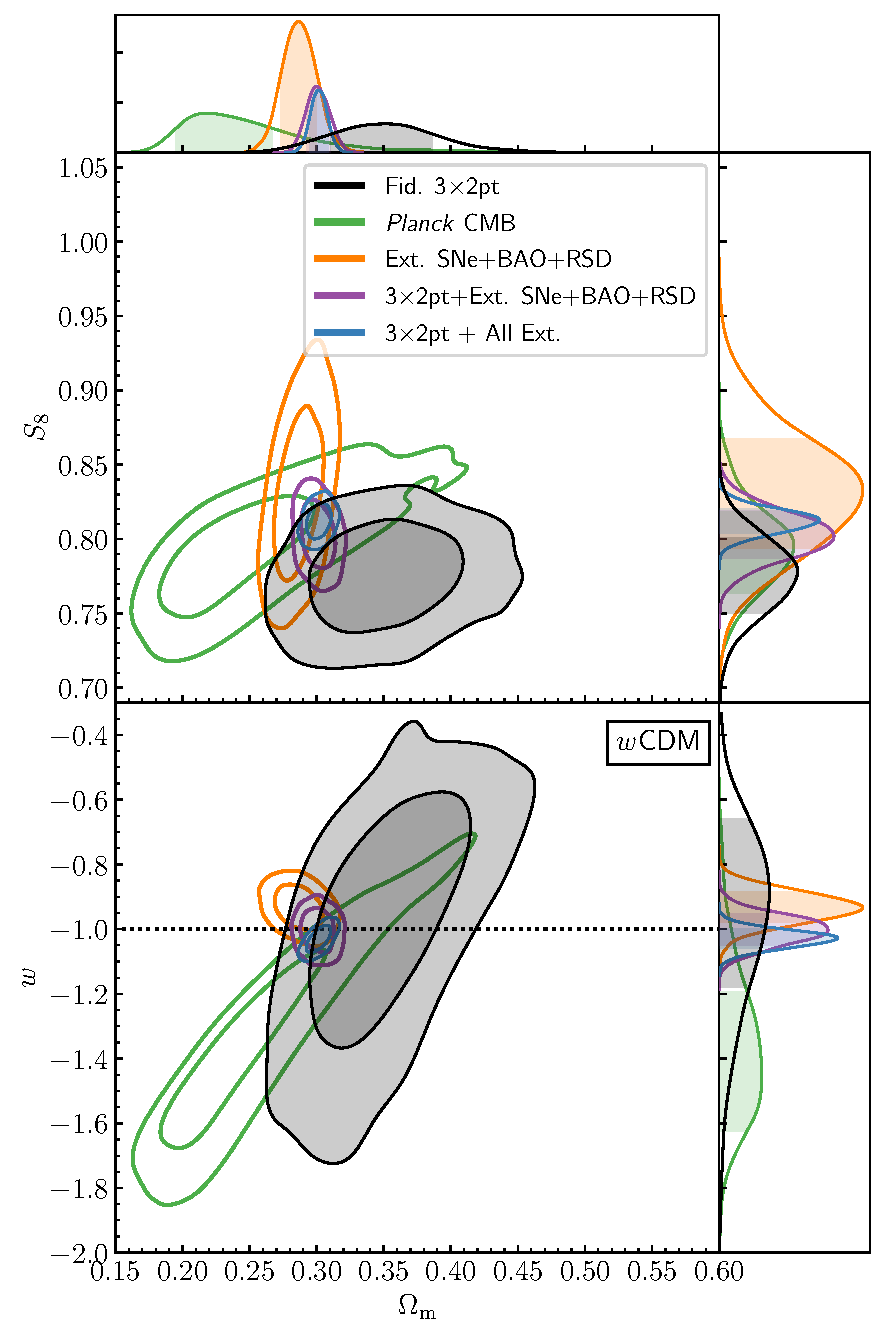
\includegraphics[width=.8\textwidth]{des_y3}
\caption{Cosmological constraints from the Dark Energy Survey Year 3 analysis \citep{DES2021}. Each panel shows the 68\% and 95\% credible regions of joint constraints on two parameters marginalised over all other parameters. The grey contours show the constraints from DES data alone, while the blue constraints include \Planck{} CMB data, baryon acoustic oscillations, redshift-space distortions and Type Ia supernovae. Other colours show other combinations of data.}
\label{co_Fig:des_y3}
\end{figure}

The Dark Energy Survey (DES; \citealt{DES2005}) is a six-year optical imaging survey on the Dark Energy Camera \citep{Flaugher2015} at the Blanco 4\,m telescope at the Cerro Tololo Inter-American Observatory in Chile. 300 million galaxies were observed between 2013 and 2019, but to date only 100 million have been included in published cosmological analyses \citep{DES2021}. The survey covers $5000\,\text{deg}^2$ and includes galaxies out to redshift $z = 2$. The Year 3 cosmological analysis reports results of $S_8 = 0.775\substack{+0.026\\-0.024}$ and $w = -0.98\substack{+0.32\\-0.20}$, from DES data alone. Combined with \Planck{} CMB data, plus baryon acoustic oscillations, redshift-space distortions and Type Ia supernovae, they obtain $S_8 = 0.812 \pm 0.08$; $w = -1.031\substack{+0.030\\-0.027}$; $h = 0.687\substack{+0.006\\-0.007}$. Some parameter constraints from the Year 3 analysis are shown in \autoref{co_Fig:des_y3}. To obtain these results, such methodological advances were necessary that the collaboration published 29 methods papers for the Year 3 analysis alone \citep[and references therein]{DES2021}. The future Year 6 analysis will require still further refinement to reliably extract the maximum information from all 300 million sources.

\subsection{\Euclid{} satellite}
\label{co_Sec:Euclid}

\Euclid{} \citep{Laureijs2011} is an upcoming European Space Agency (ESA) satellite mission. It was born from a combination of two satellite proposals to ESA: the Dark Universe Explorer (DUNE; \citealt{Refregier2009}), a weak lensing mission, and the Spectroscopic All Sky Cosmic Explorer (SPACE; \citealt{Cimatti2009}), a spectroscopic galaxy clustering mission to measure baryon acoustic oscillation and redshift-space distortions. As such, \Euclid{} is equipped with two complementary instruments: an optical imager---VIS---and a near-infrared spectrometer \& photometer---NISP. \Euclid{} is scheduled to be launched in early 2023 from the ESA spaceport in French Guiana, into an orbit around the $L_2$ Sun--Earth Lagrange point.

Over a nominal lifetime of six years, \Euclid{} will survey $15\,000\,\text{deg}^2$ of the extragalactic sky (the Euclid Wide Survey; \citealt{Scaramella2021}) out to a magnitude of 26.2 with VIS and 24.5 with NISP.
It is expected to survey around 10 billion galaxies in total, with around 1.5 billion having sufficiently precise shape and photometric redshift estimates for use in the weak lensing analysis. These source galaxies will have redshifts out to $z \sim 2$, with the majority having $z \sim 1$. Around 23 million galaxies will have precise spectroscopic redshift estimates made using NISP. There will also be three deep fields, together covering $40\,\text{deg}^2$ to form the Euclid Deep Survey, which will reach about two magnitudes deeper than the wide survey.

\begin{figure}
\centering
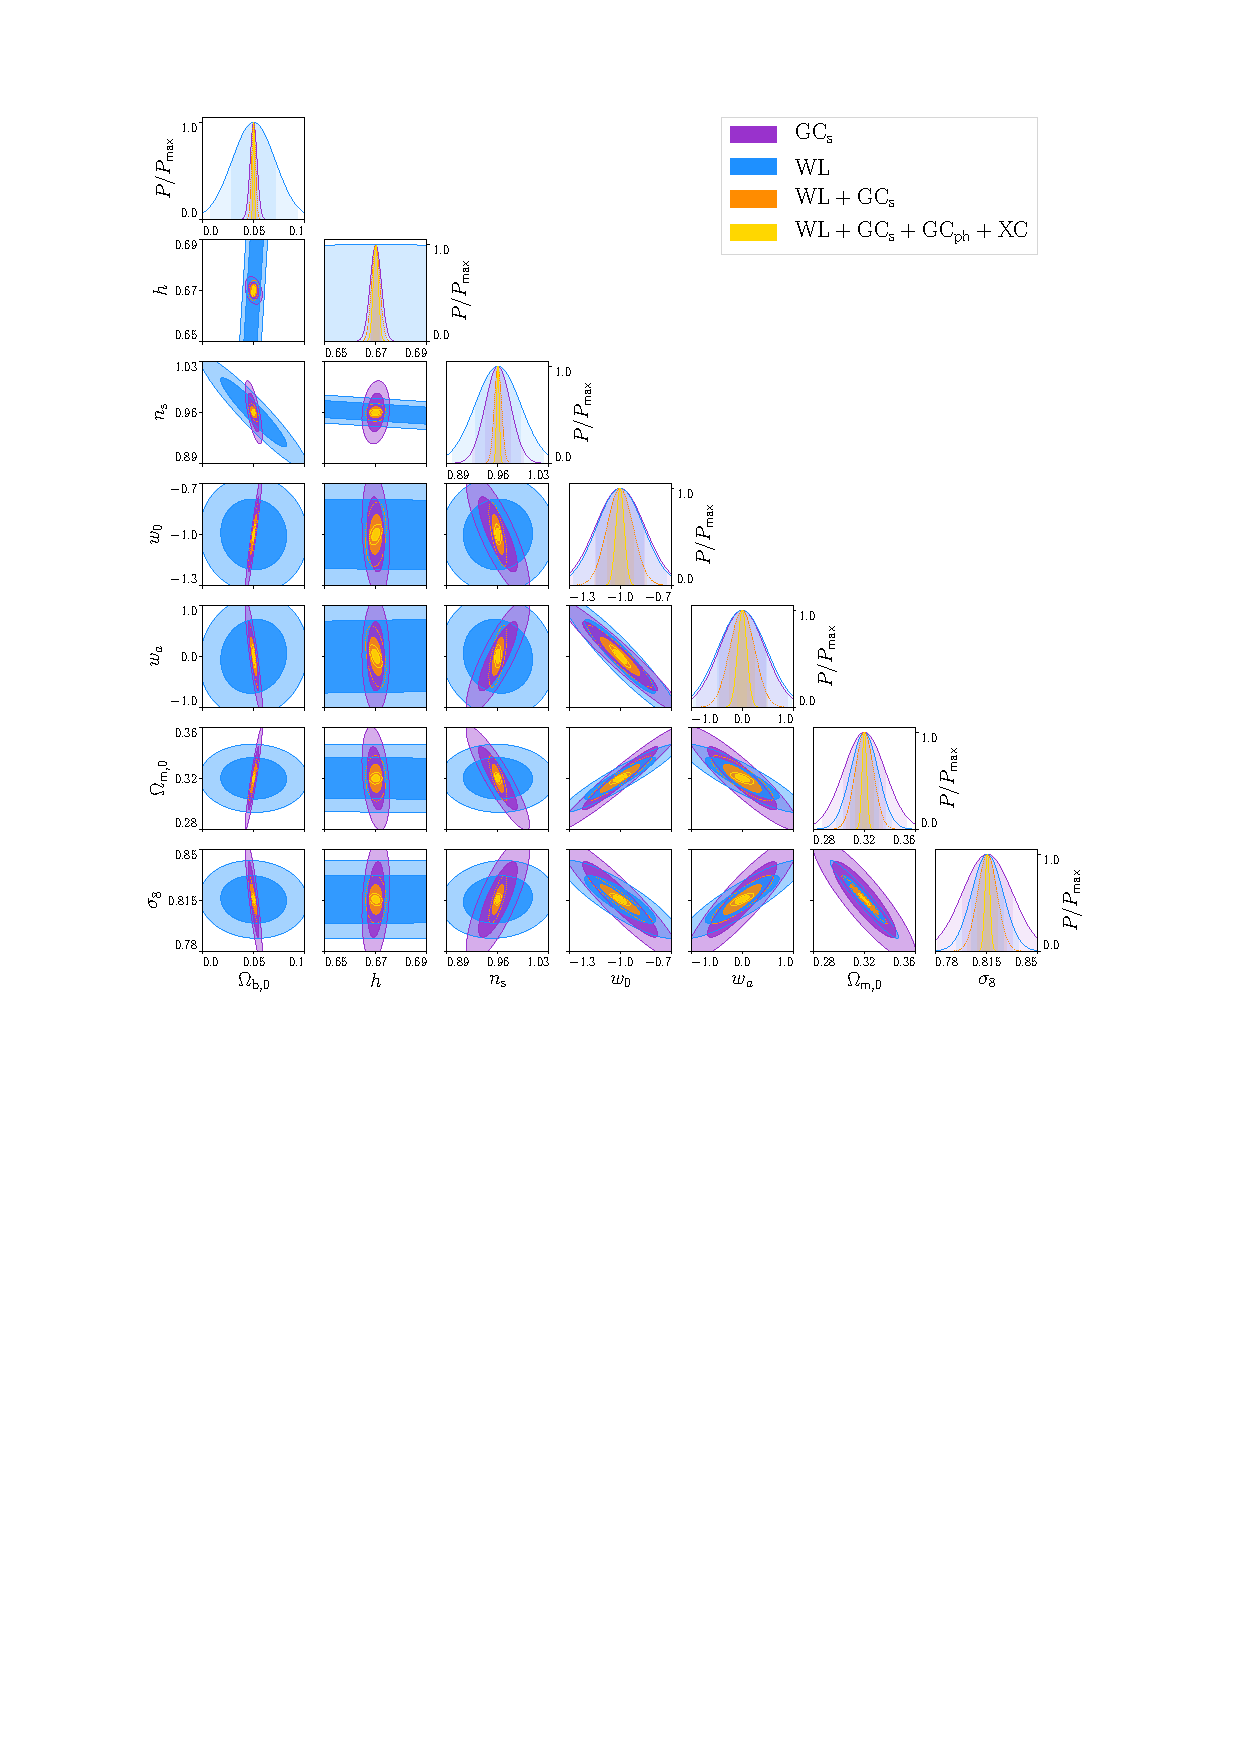
\includegraphics[width=\textwidth]{euclid_forecast}
\caption{Forecasted constraints for \wcdm{} parameters from future \Euclid{} data, combining spectroscopic galaxy clustering (GC${}_\text{s}$), weak lensing (WL), photometric galaxy clustering (GC${}_\text{ph}$) and cross-correlations (XC). Taken from \citet{Blanchard2020}.}
\label{co_Fig:euclid_forecast}
\end{figure}

The \Euclid{} cosmological analysis will use weak lensing and spectroscopic galaxy clustering, plus photometric galaxy clustering and its cross-correlation with weak lensing \citep{Blanchard2020}. Using these probes, it will determine the late-time evolution of the large-scale matter distribution in the Universe, and measure baryon acoustic oscillations and redshift-space distortions. The main scientific goal is to constrain dark energy, constraints on which are expected to improve by over an order of magnitude relative to current Stage III surveys \citep{Harrison2016}. \Euclid{} will also be able to tightly constrain other parameters of the \wcdm{} model, as shown in \autoref{co_Fig:euclid_forecast}, as well as theories of modified gravity.

The preparation and initial data analysis is conducted by the Euclid Consortium, which currently contains over 1400 people in 17 countries globally. After the initial analysis, data will be released to the public, where it is expected to have a big impact on legacy science. Potential non-cosmology uses include studies of galactic physics, and stellar physics within the Milky Way.

\subsection{Other future surveys}
\label{co_Sec:future_wl_surveys}

There are at least three other Stage IV weak lensing surveys planned alongside \Euclid{}. The first is the Vera C. Rubin Observatory Legacy Survey of Space and Time (LSST; formerly the Large Synoptic Survey Telescope; \citealt{Ivezic2019}). Rubin is a brand new ground-based observatory in Chile, which will conduct an optical imaging survey of around $18\,000\,\text{deg}^2$ of the southern sky. It has similar goals to \Euclid{} of constraining dark energy and structure growth, with some complementary characteristics; for example, \Euclid{} will have higher angular resolution, but Rubin will be able to detect fainter objects. This means that there is great potential from combining data from the two experiments \citep{Rhodes2017, Guy2022}. The survey is scheduled to last for ten years, starting in 2023.

\Euclid{} is expected to be joined at the $L_2$ point by the Nancy Grace Roman Space Telescope (formerly the Wide-Field Infrared Survey Telescope; \citealt{Spergel2015}), a NASA satellite currently scheduled to launch by May 2027. It will carry two instruments: a wide-field optical and near-infrared camera used primarily for a galaxy survey, alongside a coronograph for directly imaging exoplanets. Like \Euclid{} and Rubin, the main cosmological aim of Roman is to constrain dark energy. To do so, it will survey around $2000\,\text{deg}^2$ of the extragalactic sky over a period of around 24 months. It will be sensitive to magnitudes up to 28.5, so should be able to detect fainter galaxies than \Euclid{}, with a superior angular resolution due to its larger telescope, to compensate for the smaller survey area.

Finally, the Square Kilometre Array (SKA; \citealt{SKA2020}) is expected to be able to perform weak lensing analyses using radio observations. The SKA is a radio array currently under construction in Australia and South Africa, expected to begin observations in some capacity in the next decade. Use of the SKA for weak lensing has several key advantages compared to optical surveys such as \Euclid{} \citep{Harrison2016}: it will probe a broader redshift distribution, potentially out to $z \sim 6$; there is less PSF contamination for radio observations; intrinsic alignments may be able to be directly measured using radio polarisation \citep{Brown2011, Whittaker2015}; and it has the ability to access more of the sky, since the Galaxy is effectively transparent to radio interferometers. However, the greatest benefits are gained by cross-correlating radio and optical data, since this not only unlocks additional constraining power but also significantly reduces the impact of systematic errors, which are largely different for radio and optical surveys \citep{Camera2017}.


% % Uncomment to build alone without subfiles:
% \emergencystretch=.5em % to avoid overfull hboxes
% \printbibliography[heading=bibintoc]
% \end{document}

% 
% Uncomment to build this alone without subfiles:
% (also stuff at bottom)
\documentclass{scrbook}
% Koma script document options
\KOMAoption{paper}{a4}
\KOMAoption{fontsize}{11pt}
\KOMAoption{parskip}{half-} % paragraph spacing
% \KOMAoption{numbers}{enddot} % dot after section number
\KOMAoption{cleardoublepage}{plain} % include page numbers on blank pages
\KOMAoption{chapterprefix}{true} % 'Chapter' before number

% Packages
\usepackage{amsmath} % Gives \text command inside maths blocks
\usepackage{amssymb} % Various maths symbols
\usepackage{array} % Table formatting
\usepackage{bm} % Bold maths including Greek
\usepackage[format=plain]{caption} % Font sizing and alignment in captions
\usepackage{enumitem} % Allows numbering like 1.1 in ordered lists
% \usepackage{float} % Allows H placement of floats
\usepackage{graphicx}
\usepackage[hidelinks]{hyperref} % Hyperlinks without looking like it
% \usepackage{longtable} % Multi-page tables
% \usepackage{multicol} % For columns in text (not tables)
\usepackage{multirow} % For tables
\usepackage{neuralnetwork} % Neural net diagram
\usepackage{pdflscape} % Gives landscape environment
% \usepackage{scrlayer-scrpage} % To move page numbers
\usepackage{tabularx}
\usepackage{textcomp} % Added to fix \textasciiacute error on laptop
% \usepackage{tikz} % Diagrams (used for neural network example)
% \usepackage[pagenumberwidth=3em]{tocbasic}
% \usepackage{tocstyle} % ToC styling
\usepackage{upgreek} % Non-italic greek letters
\usepackage{xpatch} % Biblatex customisation

\usepackage[a4paper, inner=40mm, outer=15mm, top=30mm, bottom=30mm,footskip=15mm, headsep=15mm]{geometry}
% \usepackage[a4paper, inner=40mm, outer=30mm, top=50mm, bottom=50mm,footskip=20mm, headsep=20mm]{geometry} % footskip is space between footer (i.e. page number) and bottom of text
% min allowed is inner 40 mm, others 15 mm

\pagestyle{plain} % no header for front matter, overridden at end of front matter

% Caption setup
% \tablecaptionabove
\captionsetup[table]{labelsep=space}
% \captionsetup[table]{labelsep=space, skip=50pt, position=top}
\captionsetup[figure]{labelsep=space} % labelsep prevents dot followed by colon in captions

% Line spacing
\usepackage{setspace}
% \setstretch{1.4} % strangely this is > \onehalfspacing but < \doublespacing
\onehalfspacing
% \doublespacing

\raggedbottom % prevent huge spaces between paragraphs

% % % % % % % % % % % % % % % % % % % % % % % % %
% Font setup
% \usepackage{mathpazo} % Covers maths mode too
\usepackage[sc]{mathpazo} % Covers maths mode too, sc enables small caps
% \usepackage{palatino}
\usepackage[T1]{fontenc} % 8-bit font encoding
\addtokomafont{disposition}{\rmfamily} % Use serif throughout
% % % % % % % % % % % % % % % % % % % % % % % % %

% % % % % % % % % % % % % % % % % % % % % % % % %
% Section formatting setup
% \RedeclareSectionCommand[beforeskip=0pt]{chapter}
\RedeclareSectionCommand[beforeskip=0pt, innerskip=0pt]{chapter}
\RedeclareSectionCommand[beforeskip=10pt]{subsubsection}
\RedeclareSectionCommand[afterskip=1pt]{subsubsection}
% \setcounter{secnumdepth}{\subsubsectionnumdepth} % number up to subsubsections

% No dot after chapter number (https://tex.stackexchange.com/a/484727)
\renewcommand*{\chapterformat}{%
  \mbox{\chapappifchapterprefix{\nobreakspace}\thechapter
  \IfUsePrefixLine{}{\enskip}}%
}

% In the running header, separate chapter number and name with em dash
\renewcommand*{\chaptermarkformat}{%
\chapapp~\thechapter~---~}

% Create subsubsubsection below subsubsection but above paragraph, following https://tex.stackexchange.com/a/356574

\DeclareNewSectionCommand[
  style=section,
  counterwithin=subsubsection,
  afterskip=1pt,
  beforeskip=10pt,
  % afterskip=1.5ex plus .2ex,
  % beforeskip=3.25ex plus 1ex minus .2ex,
  % afterindent=false,
  level=\paragraphnumdepth,
  tocindent=10em,
  tocnumwidth=5em
]{subsubsubsection}
\setcounter{secnumdepth}{\subsubsubsectionnumdepth}
% \setcounter{tocdepth}{\subparagraphtocdepth}
\setcounter{tocdepth}{\subsubsubsectionnumdepth}

\RedeclareSectionCommands[
  level=\numexpr\subsubsubsectionnumdepth+1\relax,
  toclevel=\numexpr\subsubsubsectiontocdepth+1\relax,
  increaselevel,
]{paragraph,subparagraph}
\RedeclareSectionCommand[
  counterwithin=subsubsubsection,
  tocindent=12em,
  tocnumwidth=6em,
  beforeskip=10pt,
  afterskip=1pt, % line break after paragraph title
]{paragraph}
\RedeclareSectionCommand[
  tocindent=14em,
  tocnumwidth=7em,
  beforeskip=0pt
]{subparagraph}
% % % % % % % % % % % % % % % % % % % % % % % % %

% Autoref capitalisation
\def\chapterautorefname{Chapter}
\def\sectionautorefname{Section}
\def\subsectionautorefname{Section}
\def\subsubsectionautorefname{Section}

% % % % % % % % % % % % % % % % % % % % % % % % %
% Bibliography setup
\usepackage[backend=biber,
    % style=authoryear,
    style=authoryear-comp, % Don't repeat same author(s) in multiple citations
    giveninits=true,
    useprefix=true, % 'van der' etc.
    url=false,
    doi=false,
    isbn=false,
    eprint=false,
    uniquename=false, % Don't add initials in citation to disambiguate between authors with the same surname
    uniquelist=false, % Don't disambiguate in citation between different 'et al.' teams
    maxbibnames=10,
    minbibnames=10,
    maxcitenames=3,%  # 2,
    natbib, % Gives citep and citet commands
    labelalpha=true, % Use an 'alpha' label for each bib entry
    maxalphanames=1, % Use first author as the alpha label
    sorting=anyvt, % Sort by alpha (first author) then year
    block=par, % New line between 'blocks' of the bib entry
    dashed=false, % Reprint author list for each publication in bibliography
    sortcites=false % Show citations in the order supplied
]{biblatex}

% Citation/reference parameters
\renewcommand*{\nameyeardelim}{\addspace} % Space between author and year rather than comma
\renewcommand*{\finalnamedelim}{\addspace\&\addspace} % Ampersand rather than 'and'
\xpatchbibmacro{name:andothers}{{\finalandcomma}}{\addspace}{}{} % Space before 'et al.' rather than comma

% Citation-specific parameters
\DeclareCiteCommand{\blindcite}{\unspace}{}{}{\mancite} % Easy manual citations

% Reference-specific parameters
\AtEveryBibitem{\clearfield{title}} % Suppress title
\AtEveryBibitem{\clearfield{month}} % Suppress month
\DeclareNameAlias{author}{family-given} % Surname first for not just the first author
\DeclareNameAlias{editor}{family-given} % Same for editors
\renewbibmacro{in:}{} % Remove 'In:'
\DeclareFieldFormat{journaltitle}{#1} % Journal title in normal font rather than italics
\renewbibmacro*{volume+number+eid}{\printfield{volume}\printfield{number}\setunit{\addcomma\space}\printfield{eid}} % No dot after issue
\DeclareFieldFormat[article]{number}{\mkbibparens{#1}} % Volume in brackets
\DefineBibliographyStrings{english}{page = {}, pages = {}} % Suppress 'p.'/'pp.'
\renewbibmacro*{date+extradate}{\printtext{\printfield{year}\addcomma}} % Year not in brackets
\DeclareFieldFormat{pages}{\mkfirstpage[{\mkpageprefix[bookpagination]}]{#1}} % Only give starting page
\DeclareFieldFormat{url}{\url{#1}} % No 'URL' before URLs
% \renewcommand{\finentrypunct}{} % Remove final full stop
\renewcommand*{\newunitpunct}{\addcomma\space} % Commas between elements of bibitems

\DeclareBibliographyDriver{book}{%
  \printnames{author}%
  \space
  \printfield{year}%
  \newunit\newblock
  \printfield{booktitle}%
  \newunit
  , \printlist{publisher}%
\finentry}

\DeclareBibliographyDriver{inproceedings}{%
  \printnames{author}%
  \space
  \printfield{year}%
  \newunit\newblock
  \printfield{booktitle}%
  \newunit
  \printfield{volume}%
  \newunit
  \printfield{pages}%
\finentry}

\DeclareBibliographyDriver{incollection}{%
  \printnames{author}%
  \space
  \printfield{year}%
  \newunit\newblock
  \printfield{booktitle}%
  \newunit
  , ed. \printnames{editor},%
  \newunit\newblock
  \printlist{publisher}%
\finentry}

\DeclareBibliographyDriver{misc}{%
  \printnames{author}%
  \space
  \printfield{year}%
  \newunit\newblock
  \printfield{title}%
  \newunit
  \printfield{url}%
\finentry}

\addbibresource{refs.bib}
% % % % % % % % % % % % % % % % % % % % % % % % %

% Footnote spacing
% \deffootnote[1em]{1.5em}{1em}{\textsuperscript{\thefootnotemark~}}
\deffootnote[1em]{1em}{1em}{\textsuperscript{\thefootnotemark~}}

% Testing setting all penalties to zero
\binoppenalty=0
\brokenpenalty=0
\clubpenalty=0
\displaywidowpenalty=0
\exhyphenpenalty=0
\floatingpenalty=0
\hyphenpenalty=0
\interlinepenalty=0
% \linepenalty=0 % allowing this to be zero splits titles in a strange way
\postdisplaypenalty=0
\predisplaypenalty=0
\relpenalty=0
\widowpenalty=0

% Shorthands (non-Maths)
\newcommand{\lcdm}{$\Lambda$CDM}
\newcommand{\wcdm}{$w$CDM}
\newcommand{\Euclid}{\textit{Euclid}}
\newcommand{\Planck}{\textit{Planck}}
\newcommand{\Pcl}{Pseudo-$C_\ell$}
\newcommand{\pcl}{pseudo-$C_\ell$}
\newcommand{\ttp}{3$\times$2\,pt}

% Maths shorthands
\newcommand{\alm}{a_{\ell m}}
\newcommand{\Cl}{C_\ell}
\newcommand{\fsky}{f_\text{sky}}
\newcommand{\lmax}{\ell_\text{max}}
\newcommand{\lmin}{\ell_\text{min}}
\newcommand{\leff}{\ell_\text{eff}}
\newcommand{\tmin}{\theta_\text{min}}
\newcommand{\mathbfit}[1]{\bm{\mathit{#1}}}
\newcommand{\mathbfss}[1]{\bm{\mathsf{#1}}} % to match MNRAS \mathbfss
\renewcommand{\Re}{\operatorname{Re}}
\renewcommand{\Im}{\operatorname{Im}}

% ΛCDM parameters (maths mode)
\newcommand{\wo}{w_0}
\newcommand{\wa}{w_a}
\newcommand{\omm}{\Omega_\text{m}}
\newcommand{\omb}{\Omega_\text{b}}
\newcommand{\omc}{\Omega_\text{c}}
\newcommand{\sie}{\sigma_8}

% % Editing only
% \usepackage{xcolor}
% \newcommand{\todo}[1]{\textbf{{\color{red}{#1}}}}


% \usepackage{subfiles} % Best to do this last apparently

\pagestyle{headings}
\setcounter{chapter}{0} % deliberately 1 too low
\begin{document}

% Uncomment to use subfiles:
% \documentclass[../Thesis.tex]{subfiles}
% \begin{document}

\chapter{Cosmology}

Cosmology is the study of the Universe, the components that make it up, and its past and future evolution. Our understanding of these topics has improved greatly over the past century, beginning with the development of the theory of general relativity (GR), which describes gravity as an emergent phenomenon resulting from the effect of mass on the geometry of spacetime \citep{Einstein1916}. Solutions to GR were later developed \citep{Friedmann1922, Friedmann1924, Lemaitre1927, Lemaitre1933, Robertson1935, Robertson1936a, Robertson1936b, Walker1937} to describe an expanding universe that is homogeneous and isotropic. Meanwhile, observational evidence for universal expansion was provided by the discovery of `Hubble's law', which states that distant galaxies are moving away from Earth at a speed proportional to their distance \citep{Lemaitre1927, Hubble1929}.

The application of time symmetry to the expanding Universe implies that it has a finite age, and that the early Universe was extremely dense. This became known as the `Big Bang' model. An important prediction of the model is the existence of the cosmic microwave background radiation (CMB; see \autoref{Sec:cmb_intro}) \citep{Gamow1948a, Gamow1948b, Alpher1948a, Alpher1948b}, which was discovered in 1965 \citep{Penzias1965, Dicke1965}. Later observations of the CMB with the Cosmic Background Explorer (COBE) satellite confirmed that it has an almost perfect blackbody spectrum \citep{Mather1990, Mather1994, Fixsen1996}, providing perhaps the strongest evidence for the Big Bang model.

Meanwhile, it was deduced from observations of the orbital speeds of stars in nearby galaxies that an additional invisible `dark' form of matter must exist \citep{Kapteyn1922, Zwicky1933, Zwicky1937, Rubin1970, Freeman1970, Bosma1978}. It was later found that dark matter must be non-relativistic (`cold') and that it dominates the matter content of the Universe \citep{Rubin1980, Bond1982, Blumenthal1982, Davis1985}.

Since the Universe was known both to be expanding and to contain large amounts of gravitationally attractive matter, it was broadly expected that the expansion should be decelerating \citep[e.g.][]{Yoshii1988, Gasperini1993}. However, measurements of the deceleration rate derived from observations of distant supernova at the end of the last century revealed that the expansion of the Universe is in fact accelerating \citep{Riess1998, Perlmutter1999}. This was the most recent major change in our understanding of the Universe, and led to the development of the current standard model of cosmology (see \autoref{Sec:std_model} below) and to the era widely described as that of `precision cosmology' \citep[e.g.][]{Steigman2007}, though this perhaps belies the fact that the nature of so much of the Universe remains a mystery (see \autoref{Sec:open_questions}).

\section{Standard cosmological model}
\label{Sec:std_model}

The simplest cosmological model that is broadly consistent with all observations to date is the \lcdm{} model. $\Lambda$ represents the cosmological constant, which is an additional contribution to the energy density of the Universe that is constant with space and time---the simplest model of the `dark energy' required to account for the observed accelerating expansion. CDM stands for cold dark matter. These two dominant components of the Universe, dark energy and dark matter, constitute a respective 68.3\% and 26.8\% of the energy of the Universe. The remainder is mostly `baryonic' matter---normal matter as we know it on Earth, with very small contributions from the CMB and cosmic neutrinos.

The \lcdm{} Universe evolves following GR and its solutions for an expanding Universe that is homogeneous and isotropic on large scales, which are contained in the Friedmann equations \citep{Friedmann1922,Friedmann1924}. It is spatially flat, obeying Euclidean geometry. The remainder of the model is fitted to a minimal number of six parameters. However, the model can be extended by additional parameters to describe more complex behaviour, such as spatial curvature and time-dependent dark energy.

\subsection{Dark energy}

In \lcdm{} and its extensions, the components of the Universe are modelled as perfect fluids that can be characterised completely by their energy density $\rho$ and pressure $p$. The ratio of pressure to density is the dimensionless equation of state parameter $w$:
\begin{equation}
w = \frac{p}{\rho}.
\end{equation}
Unless otherwise specified, in this thesis $w$ will refer to the ratio of pressure to density for dark energy specifically.

If dark energy can be described by a cosmological constant, then
\begin{equation}
w = -1.
\end{equation}
The simplest extension is to allow $w$ to take a constant value other than -1. Alernatively, we can allow $w$ to vary with time, parametrised using the scale factor $a$, where $a = 0$ at the Big Bang and $a = 1$ today. Taylor expanding to linear order around a present value of $w_0$ gives
\begin{equation}
w \left( a \right) = w_0 + w_a \left( 1 - a \right),
\end{equation}
where
\begin{equation}
w_a = - \frac{dw}{da}.
\end{equation}

\section{Outstanding questions}
\label{Sec:open_questions}

Even if \lcdm{} is correct, it leaves many questions unanswered, including the physical nature of its dominant components. The physical form of dark matter is unknown: many theories exist, and current observations still permit a large range of different explanations \citep{Khimey2021}. Meanwhile, attempts to produce and directly detect dark matter in particle colliders have so far been unsuccessful \citep{Trevisani2018}. Even less is known of dark energy. It may be a constant vacuum energy, but the vacuum energy predicted by the standard model of particle physics is 120 orders of magnitude too large \citep[e.g][]{Carroll2001}. Alternatively it may be an additional scalar field, a class of theories known as `quintessence' \citep{Ratra1988, Caldwell1998, Carroll1998, Zlatev1999, Amendola2000}. Baryonic matter is comparatively well understood, but theories predict that there should be as much antimatter in the Universe as matter, contrary to all observations \citep{Sakharov1967, Steigman2018}.

Additionally, as the free parameters of the model are measured with increasing precision, tensions have emerged between values derived by different methods. The largest is the disagreement in the Hubble parameter $H_0$, which quantifies the current expansion rate of the Universe. $H_0$ can be directly estimated by measuring the redshifts of distant galaxies and determining their distance using `standard candles' of known brightness, typically Cepheid variables and Type IA supernovae. Alternatively, an estimate of $H_0$ can be derived from measurements of the cosmic microwave background. The two methods disagree, with a statistical significance of over $4 \sigma$ \citep{Planck2018VI, Riess2019, Verde2019}.

Finally, the model itself may simply be wrong. For example, it could be that one of its foundations, GR, is not correct, and that a modified theory of gravity is required---which may negate the need for dark energy to explain the accelerating expansion of the Universe \citep{Clifton2012, Joyce2016}. While \lcdm{} is able to explain all observations to date, it will continue to be tested with ever-increasing precision by a variety of methods, which will be described in the next section.

\section{Observational probes}

There are many observational methods by which we have learned and hope to continue to learn about the nature of the Universe, some of which are described in this section.

\subsection{Cosmic microwave background}
\label{Sec:cmb_intro}

In the early Universe (up to around 370\,000 years after the Big Bang), the temperature was so high that matter existed only in an ionised state, as separate protons and electrons, in a thermal equilibrium with photons. If an atom formed, it was reionised essentially immediately by a high-energy photon. As the Universe expanded, it cooled, and at a certain point photons no longer had sufficient energy to ionise matter. Since this point---known as recombination---the vast majority of these photons have travelled through the Universe with no or minimal interactions with other matter or radiation. They have continued to cool as the Universe has expanded, and today form the cosmic microwave background (CMB).

The CMB has very small anisotropies, due to quantum fluctuations in the early Universe. The \lcdm{} model predicts the distribution of these anisotropies depending on the values of the free parameters in the model. Successive satellite missions---COBE (1989--1993), the Wilkinson Microwave Anisotropy Probe (WMAP; 2001--2010), and \textit{Planck} (2009--2013)---have measured the anisotropies with increasing precision \citep{Bennett1996, Komatsu2011, Planck2015XIII}. The final cosmological analysis of the \textit{Planck} mission in 2018 provided the most precise cosmological constraints to date \citep{Planck2018VI}.

Some future CMB experiments are aimed at measuring its polarisation with increased precision, which may lead to a detection of the first clear evidence of cosmic inflation \citep{Kamionkowski2016}. Others aim to measure spectral distortions: deviations from a blackbody spectrum occuring due to interactions between CMB photons and other matter or radiation, which can potentially offer insight into all epochs of the Universe from recombination to the present day \citep{Chluba2021}.


Future CMB experiments are aimed at what exactly? inflation (B-modes), spectral distortions?

 without interacting

- where does the cmb come from

- as

and how they can relate to the outstanding questions

- cmb

- particle detectors detecting extraterrestrial particles, plus colliders

- strong lensing can differentiate between models of DM, maybe gravity too

- LSS other than lensing

- perhaps BAO or something should be mentioned, because really this section should be tied to a) how we know what we know and b) how we hope to know what we don't know

how we know what we know:

- expansion: supernovae

- more or less everything else lol: CMB

- but I think BAOs are relevant too

- yeah ok apparently the Planck 2018 results are CMB + SN + BAOs

...

- weak lensing, which gets a section to itself

\section{Weak gravitational lensing}


% Uncomment to build alone without subfiles:
\printbibliography[heading=bibintoc]
\end{document}


% Cosmological estimators and likelihoods

% % Uncomment to build this alone without subfiles:
% % (also stuff at bottom)
% \documentclass{scrbook}
% % Koma script document options
\KOMAoption{paper}{a4}
\KOMAoption{fontsize}{11pt}
\KOMAoption{parskip}{half-} % paragraph spacing
% \KOMAoption{numbers}{enddot} % dot after section number
\KOMAoption{cleardoublepage}{plain} % include page numbers on blank pages
\KOMAoption{chapterprefix}{true} % 'Chapter' before number

% Packages
\usepackage{amsmath} % Gives \text command inside maths blocks
\usepackage{amssymb} % Various maths symbols
\usepackage{array} % Table formatting
\usepackage{bm} % Bold maths including Greek
\usepackage[format=plain]{caption} % Font sizing and alignment in captions
\usepackage{enumitem} % Allows numbering like 1.1 in ordered lists
% \usepackage{float} % Allows H placement of floats
\usepackage{graphicx}
\usepackage[hidelinks]{hyperref} % Hyperlinks without looking like it
% \usepackage{longtable} % Multi-page tables
% \usepackage{multicol} % For columns in text (not tables)
\usepackage{multirow} % For tables
\usepackage{neuralnetwork} % Neural net diagram
\usepackage{pdflscape} % Gives landscape environment
% \usepackage{scrlayer-scrpage} % To move page numbers
\usepackage{tabularx}
\usepackage{textcomp} % Added to fix \textasciiacute error on laptop
% \usepackage{tikz} % Diagrams (used for neural network example)
% \usepackage[pagenumberwidth=3em]{tocbasic}
% \usepackage{tocstyle} % ToC styling
\usepackage{upgreek} % Non-italic greek letters
\usepackage{xpatch} % Biblatex customisation

\usepackage[a4paper, inner=40mm, outer=15mm, top=30mm, bottom=30mm,footskip=15mm, headsep=15mm]{geometry}
% \usepackage[a4paper, inner=40mm, outer=30mm, top=50mm, bottom=50mm,footskip=20mm, headsep=20mm]{geometry} % footskip is space between footer (i.e. page number) and bottom of text
% min allowed is inner 40 mm, others 15 mm

\pagestyle{plain} % no header for front matter, overridden at end of front matter

% Caption setup
% \tablecaptionabove
\captionsetup[table]{labelsep=space}
% \captionsetup[table]{labelsep=space, skip=50pt, position=top}
\captionsetup[figure]{labelsep=space} % labelsep prevents dot followed by colon in captions

% Line spacing
\usepackage{setspace}
% \setstretch{1.4} % strangely this is > \onehalfspacing but < \doublespacing
\onehalfspacing
% \doublespacing

\raggedbottom % prevent huge spaces between paragraphs

% % % % % % % % % % % % % % % % % % % % % % % % %
% Font setup
% \usepackage{mathpazo} % Covers maths mode too
\usepackage[sc]{mathpazo} % Covers maths mode too, sc enables small caps
% \usepackage{palatino}
\usepackage[T1]{fontenc} % 8-bit font encoding
\addtokomafont{disposition}{\rmfamily} % Use serif throughout
% % % % % % % % % % % % % % % % % % % % % % % % %

% % % % % % % % % % % % % % % % % % % % % % % % %
% Section formatting setup
% \RedeclareSectionCommand[beforeskip=0pt]{chapter}
\RedeclareSectionCommand[beforeskip=0pt, innerskip=0pt]{chapter}
\RedeclareSectionCommand[beforeskip=10pt]{subsubsection}
\RedeclareSectionCommand[afterskip=1pt]{subsubsection}
% \setcounter{secnumdepth}{\subsubsectionnumdepth} % number up to subsubsections

% No dot after chapter number (https://tex.stackexchange.com/a/484727)
\renewcommand*{\chapterformat}{%
  \mbox{\chapappifchapterprefix{\nobreakspace}\thechapter
  \IfUsePrefixLine{}{\enskip}}%
}

% In the running header, separate chapter number and name with em dash
\renewcommand*{\chaptermarkformat}{%
\chapapp~\thechapter~---~}

% Create subsubsubsection below subsubsection but above paragraph, following https://tex.stackexchange.com/a/356574

\DeclareNewSectionCommand[
  style=section,
  counterwithin=subsubsection,
  afterskip=1pt,
  beforeskip=10pt,
  % afterskip=1.5ex plus .2ex,
  % beforeskip=3.25ex plus 1ex minus .2ex,
  % afterindent=false,
  level=\paragraphnumdepth,
  tocindent=10em,
  tocnumwidth=5em
]{subsubsubsection}
\setcounter{secnumdepth}{\subsubsubsectionnumdepth}
% \setcounter{tocdepth}{\subparagraphtocdepth}
\setcounter{tocdepth}{\subsubsubsectionnumdepth}

\RedeclareSectionCommands[
  level=\numexpr\subsubsubsectionnumdepth+1\relax,
  toclevel=\numexpr\subsubsubsectiontocdepth+1\relax,
  increaselevel,
]{paragraph,subparagraph}
\RedeclareSectionCommand[
  counterwithin=subsubsubsection,
  tocindent=12em,
  tocnumwidth=6em,
  beforeskip=10pt,
  afterskip=1pt, % line break after paragraph title
]{paragraph}
\RedeclareSectionCommand[
  tocindent=14em,
  tocnumwidth=7em,
  beforeskip=0pt
]{subparagraph}
% % % % % % % % % % % % % % % % % % % % % % % % %

% Autoref capitalisation
\def\chapterautorefname{Chapter}
\def\sectionautorefname{Section}
\def\subsectionautorefname{Section}
\def\subsubsectionautorefname{Section}

% % % % % % % % % % % % % % % % % % % % % % % % %
% Bibliography setup
\usepackage[backend=biber,
    % style=authoryear,
    style=authoryear-comp, % Don't repeat same author(s) in multiple citations
    giveninits=true,
    useprefix=true, % 'van der' etc.
    url=false,
    doi=false,
    isbn=false,
    eprint=false,
    uniquename=false, % Don't add initials in citation to disambiguate between authors with the same surname
    uniquelist=false, % Don't disambiguate in citation between different 'et al.' teams
    maxbibnames=10,
    minbibnames=10,
    maxcitenames=3,%  # 2,
    natbib, % Gives citep and citet commands
    labelalpha=true, % Use an 'alpha' label for each bib entry
    maxalphanames=1, % Use first author as the alpha label
    sorting=anyvt, % Sort by alpha (first author) then year
    block=par, % New line between 'blocks' of the bib entry
    dashed=false, % Reprint author list for each publication in bibliography
    sortcites=false % Show citations in the order supplied
]{biblatex}

% Citation/reference parameters
\renewcommand*{\nameyeardelim}{\addspace} % Space between author and year rather than comma
\renewcommand*{\finalnamedelim}{\addspace\&\addspace} % Ampersand rather than 'and'
\xpatchbibmacro{name:andothers}{{\finalandcomma}}{\addspace}{}{} % Space before 'et al.' rather than comma

% Citation-specific parameters
\DeclareCiteCommand{\blindcite}{\unspace}{}{}{\mancite} % Easy manual citations

% Reference-specific parameters
\AtEveryBibitem{\clearfield{title}} % Suppress title
\AtEveryBibitem{\clearfield{month}} % Suppress month
\DeclareNameAlias{author}{family-given} % Surname first for not just the first author
\DeclareNameAlias{editor}{family-given} % Same for editors
\renewbibmacro{in:}{} % Remove 'In:'
\DeclareFieldFormat{journaltitle}{#1} % Journal title in normal font rather than italics
\renewbibmacro*{volume+number+eid}{\printfield{volume}\printfield{number}\setunit{\addcomma\space}\printfield{eid}} % No dot after issue
\DeclareFieldFormat[article]{number}{\mkbibparens{#1}} % Volume in brackets
\DefineBibliographyStrings{english}{page = {}, pages = {}} % Suppress 'p.'/'pp.'
\renewbibmacro*{date+extradate}{\printtext{\printfield{year}\addcomma}} % Year not in brackets
\DeclareFieldFormat{pages}{\mkfirstpage[{\mkpageprefix[bookpagination]}]{#1}} % Only give starting page
\DeclareFieldFormat{url}{\url{#1}} % No 'URL' before URLs
% \renewcommand{\finentrypunct}{} % Remove final full stop
\renewcommand*{\newunitpunct}{\addcomma\space} % Commas between elements of bibitems

\DeclareBibliographyDriver{book}{%
  \printnames{author}%
  \space
  \printfield{year}%
  \newunit\newblock
  \printfield{booktitle}%
  \newunit
  , \printlist{publisher}%
\finentry}

\DeclareBibliographyDriver{inproceedings}{%
  \printnames{author}%
  \space
  \printfield{year}%
  \newunit\newblock
  \printfield{booktitle}%
  \newunit
  \printfield{volume}%
  \newunit
  \printfield{pages}%
\finentry}

\DeclareBibliographyDriver{incollection}{%
  \printnames{author}%
  \space
  \printfield{year}%
  \newunit\newblock
  \printfield{booktitle}%
  \newunit
  , ed. \printnames{editor},%
  \newunit\newblock
  \printlist{publisher}%
\finentry}

\DeclareBibliographyDriver{misc}{%
  \printnames{author}%
  \space
  \printfield{year}%
  \newunit\newblock
  \printfield{title}%
  \newunit
  \printfield{url}%
\finentry}

\addbibresource{refs.bib}
% % % % % % % % % % % % % % % % % % % % % % % % %

% Footnote spacing
% \deffootnote[1em]{1.5em}{1em}{\textsuperscript{\thefootnotemark~}}
\deffootnote[1em]{1em}{1em}{\textsuperscript{\thefootnotemark~}}

% Testing setting all penalties to zero
\binoppenalty=0
\brokenpenalty=0
\clubpenalty=0
\displaywidowpenalty=0
\exhyphenpenalty=0
\floatingpenalty=0
\hyphenpenalty=0
\interlinepenalty=0
% \linepenalty=0 % allowing this to be zero splits titles in a strange way
\postdisplaypenalty=0
\predisplaypenalty=0
\relpenalty=0
\widowpenalty=0

% Shorthands (non-Maths)
\newcommand{\lcdm}{$\Lambda$CDM}
\newcommand{\wcdm}{$w$CDM}
\newcommand{\Euclid}{\textit{Euclid}}
\newcommand{\Planck}{\textit{Planck}}
\newcommand{\Pcl}{Pseudo-$C_\ell$}
\newcommand{\pcl}{pseudo-$C_\ell$}
\newcommand{\ttp}{3$\times$2\,pt}

% Maths shorthands
\newcommand{\alm}{a_{\ell m}}
\newcommand{\Cl}{C_\ell}
\newcommand{\fsky}{f_\text{sky}}
\newcommand{\lmax}{\ell_\text{max}}
\newcommand{\lmin}{\ell_\text{min}}
\newcommand{\leff}{\ell_\text{eff}}
\newcommand{\tmin}{\theta_\text{min}}
\newcommand{\mathbfit}[1]{\bm{\mathit{#1}}}
\newcommand{\mathbfss}[1]{\bm{\mathsf{#1}}} % to match MNRAS \mathbfss
\renewcommand{\Re}{\operatorname{Re}}
\renewcommand{\Im}{\operatorname{Im}}

% ΛCDM parameters (maths mode)
\newcommand{\wo}{w_0}
\newcommand{\wa}{w_a}
\newcommand{\omm}{\Omega_\text{m}}
\newcommand{\omb}{\Omega_\text{b}}
\newcommand{\omc}{\Omega_\text{c}}
\newcommand{\sie}{\sigma_8}

% % Editing only
% \usepackage{xcolor}
% \newcommand{\todo}[1]{\textbf{{\color{red}{#1}}}}


% \usepackage{subfiles} % Best to do this last apparently

% \pagestyle{headings}
% \setcounter{chapter}{1} % deliberately 1 too low
% \begin{document}

% Uncomment to use subfiles:
% \documentclass[../Thesis.tex]{subfiles}
% \begin{document}

\chapter{Cosmological estimators and likelihoods}
\label{chap:est_like}

This chapter introduces some of the mathematical concepts involved in the later chapters in this thesis. It begins with an introduction to cosmological fields on the sphere in \autoref{est_Sec:cosmological_fields}, before focusing specifically on weak lensing fields and two-point statistics in \autoref{est_Sec:wl_fields}. \autoref{est_Sec:pcl} introduces the \pcl{} method, which is central to much of the work presented in this thesis, before the concepts of Bayesian inference and likelihoods are described in \autoref{est_Sec:inference}.

This chapter has been compiled from \citet{Heavens2003, Chon2004, Brown2005, Kilbinger2017, Chisari2019, Fang2020b}.

\section{Cosmological fields on the sphere}
\label{est_Sec:cosmological_fields}

The sky as viewed from the Earth, or indeed anywhere, may be modelled as a sphere (though one can only see up to half the sphere from a fixed point on the surface of the Earth at any given instant). As a result, astronomical observations may be described as fields on the sphere. In the context of cosmology, cosmic variance (introduced in \autoref{chap:cosmo}) means that cosmological fields are modelled as random fields on the sphere. The cosmological principle requires that these fields are statistically isotropic and translation invariant, meaning that information is only contained in the dependence on angular scales and not in orientation or position. Because of this property, it is often most convenient to work with spherical harmonics. For a general scalar field $\psi$, the transforms between the field in angular coordinates $\psi \left( \theta, \phi \right)$ and in spherical harmonics $\psi_{\ell m}$ are
\begin{align}
\psi_{\ell m} &= \int{\text{d}\theta \int{\text{d}\phi ~
\psi \left( \theta, \phi \right) Y_{\ell m}^* \left( \theta, \phi \right) } };
\label{est_Eqn:sht_to_alm_spin0}
\\[1em]
\psi \left( \theta, \phi \right) &= \sum_{\ell = 0}^\infty
\sum_{m = - \ell}^{+\ell} \psi_{\ell m}
Y_{\ell m} \left( \theta, \phi \right),
\label{est_Eqn:sht_from_alm_spin0}
\end{align}
where $Y_{\ell m} \left( \theta, \phi \right)$ are the spherical harmonics, and $*$ denotes complex conjugation. Equations \eqref{est_Eqn:sht_to_alm_spin0}--\eqref{est_Eqn:sht_from_alm_spin0} are the spin-0 spherical harmonic transforms (spin will be discussed in \autoref{est_Sec:spin}).

Statistical isotropy implies that only the degree $\ell$ and not the order $m$ carries cosmological information. The field is then mostly characterised by the angular power spectrum $C_\ell$, defined as the expectation value of the product of spherical harmonic coefficients,
\begin{equation}
\left\langle \psi_{\ell m} \psi^*_{\ell' m'} \right\rangle
= \delta_{\ell \ell'} \delta_{m m'} C_\ell^\psi,
\end{equation}
where $\delta$ is the Kronecker delta function.
If the field $\psi$ follows Gaussian statistics, the information content of the field is entirely contained within this power spectrum. If the field is non-Gaussian, higher-order moments are required to fully describe it.

An equivalent, alternative statistic to the angular power spectrum is the angular two-point correlation function $\xi \left( \theta \right)$, defined as
\begin{equation}
\left\langle \psi \left( \bm{\Omega} \right)
\psi \left( \bm{\Omega'} \right) \right\rangle
= \xi^\psi \left( \left| \bm{\Omega'} - \bm{\Omega} \right| \right),
\label{est_Eqn:2pcf_definition}
\end{equation}
where $\bm{\Omega}$ and $\bm{\Omega'}$ are sky coordinates. The correlation function may be obtained from the power spectrum as
\begin{equation}
\xi \left( \theta \right) = \sum_{\ell = 0}^\infty {
\frac{2 \ell + 1}{4 \pi} C_\ell \,
d^\ell_{00} \left( \theta \right) },
\end{equation}
where $d^\ell_{m' m}$ is a Wigner small-$d$ symbol.

Two correlated fields $\alpha$ and $\beta$ may be described by their cross-power spectrum $C_\ell^{\alpha \beta}$,
\begin{equation}
\left\langle \alpha_{\ell m} \beta^*_{\ell' m'} \right\rangle
= \delta_{\ell \ell'} \delta_{m m'} C_\ell^{\alpha \beta},
\label{est_Eqn:general_cross_cl}
\end{equation}
or by their cross-correlation function, defined analogously to Equation \eqref{est_Eqn:2pcf_definition}. Cross-power spectra and cross-correlation functions are symmetric such that
\begin{align}
C_\ell^{\alpha \beta} &= C_\ell^{\beta \alpha};
\\[1em]
\xi^{\alpha \beta} \left( \theta \right)
&= \xi^{\beta \alpha} \left( \theta \right).
\end{align}

\subsection{Spin}
\label{est_Sec:spin}

Some cosmological fields are scalar, in that they are described by a single value at each point on the sky. Examples include the CMB temperature anisotropies, or the number density of galaxies. These fields are spin-0, and obey the above equations.

Some cosmological fields are spin-2, such as the CMB polarisation, and weak lensing shear. These fields are described by two values at each point, such that they can be modelled as complex. A general spin-2 field $\gamma$ can be decomposed into two components $\gamma_1$ and $\gamma_2$,
\begin{equation}
\gamma = \gamma_1 + i \gamma_2,
\end{equation}
or into a magnitude $\left| \gamma \right|$ and phase $\phi$,
\begin{equation}
\gamma = \left| \gamma \right| e^{2 i \phi}.
\label{est_Eqn:spin2_complex}
\end{equation}
The factor of $2$ in Equation \eqref{est_Eqn:spin2_complex} captures the spin-2 nature of $\gamma$. It ensures that the field is invariant under
\begin{equation}
\phi \rightarrow \phi + \pi.
\end{equation}

The equivalent of Equations \eqref{est_Eqn:sht_to_alm_spin0}--\eqref{est_Eqn:sht_from_alm_spin0} for spin-2 fields are the spin-2 spherical harmonic transforms,
\begin{align}
{}_2\gamma_{\ell m} &= \int{\text{d}\theta \int{\text{d}\phi ~
\gamma \left( \theta, \phi \right)
{}_2Y_{\ell m}^* \left( \theta, \phi \right) } };
\\[1em]
{}_{-2}\gamma_{\ell m} &= \int{\text{d}\theta \int{\text{d}\phi ~
\gamma^* \left( \theta, \phi \right)
{}_{-2}Y_{\ell m}^* \left( \theta, \phi \right) } };
\\[1em]
\gamma \left( \theta, \phi \right) &= \sum_{\ell = 0}^\infty
\sum_{m = - \ell}^{+\ell} {}_2\gamma_{\ell m}
{}_2Y_{\ell m} \left( \theta, \phi \right);
\\[1em]
\gamma^* \left( \theta, \phi \right) &= \sum_{\ell = 0}^\infty
\sum_{m = - \ell}^{+\ell} {}_{-2}\gamma_{\ell m}
{}_{-2}Y_{\ell m} \left( \theta, \phi \right),
\end{align}
where ${}_sY_{\ell m} \left( \theta, \phi \right)$ are the spin-weighted spherical harmonics.

An alternative decomposition of a spin-2 field that is often more closely related to the physical origins of the field (such as in both CMB polarisation and weak lensing shear) is the decomposition into $E$-mode and $B$-mode components, as
\begin{align}
E_{\ell m} &= \frac{1}{2} \Big[ {}_2\gamma_{\ell m}
+ {}_{-2}\gamma_{\ell m} \Big];
\\[1em]
B_{\ell m} &= \frac{-i}{2} \Big[ {}_2\gamma_{\ell m}
- {}_{-2}\gamma_{\ell m} \Big].
\end{align}

It is then possible to transform directly between the spin-2 field and its $E$- and $B$-mode harmonic coefficients as
\begin{align}
E_{\ell m} &= \frac{1}{2} \int{\text{d}\theta \int{\text{d}\phi ~
\Big[ \gamma \left( \theta, \phi \right)
{}_2Y_{\ell m}^* \left( \theta, \phi \right)
+ \gamma^* \left( \theta, \phi \right)
{}_{-2}Y_{\ell m}^* \left( \theta, \phi \right) \Big] } };
\\[1em]
B_{\ell m} &= \frac{-i}{2} \int{\text{d}\theta \int{\text{d}\phi ~
\Big[ \gamma \left( \theta, \phi \right)
{}_2Y_{\ell m}^* \left( \theta, \phi \right)
- \gamma^* \left( \theta, \phi \right)
{}_{-2}Y_{\ell m}^* \left( \theta, \phi \right) \Big] } };
\\[1em]
\gamma \left( \theta, \phi \right) &= \sum_{\ell = 0}^\infty
\sum_{m = - \ell}^{+\ell} \Big[ E_{\ell m} + i B_{\ell m} \Big]
{}_2Y_{\ell m} \left( \theta, \phi \right);
\\[1em]
\gamma^* \left( \theta, \phi \right) &= \sum_{\ell = 0}^\infty
\sum_{m = - \ell}^{+\ell} \Big[ E_{\ell m} - i B_{\ell m} \Big]
{}_{-2}Y_{\ell m} \left( \theta, \phi \right).
\end{align}

We may then define the $E$-mode and $B$-mode power spectra, $C_\ell^{EE}$ and $C_\ell^{BB}$, as
\begin{align}
\left\langle E_{\ell m} E^*_{\ell' m'} \right\rangle
&= \delta_{\ell \ell'} \delta_{m m'} C_\ell^{EE};
\\[1em]
\left\langle B_{\ell m} B^*_{\ell' m'} \right\rangle
&= \delta_{\ell \ell'} \delta_{m m'} C_\ell^{BB},
\end{align}
as well as the $E$-$B$ cross-power spectrum $C_\ell^{EB}$,
\begin{equation}
\left\langle E_{\ell m} B^*_{\ell' m'} \right\rangle
= \delta_{\ell \ell'} \delta_{m m'} C_\ell^{EB}.
\end{equation}

These may be used to obtain the spin-2 $\xi^+$ and $\xi^-$ correlation functions,
\begin{equation}
\xi^\pm \left( \theta \right) = \sum_{\ell = 0}^\infty {
\frac{2 \ell + 1}{4 \pi}
\Big[ C_\ell^{EE} \pm C_\ell^{BB} \Big] \,
d^\ell_{\pm 2 2} \left( \theta \right) }.
\end{equation}

There may also be cross-power spectra between spin-0 and spin-2 fields,
\begin{align}
\left\langle \psi_{\ell m} E^*_{\ell' m'} \right\rangle
&= \delta_{\ell \ell'} \delta_{m m'} C_\ell^{\psi E};
\\[1em]
\left\langle \psi_{\ell m} B^*_{\ell' m'} \right\rangle
&= \delta_{\ell \ell'} \delta_{m m'} C_\ell^{\psi B},
\end{align}
and a corresponding cross-correlation function $\xi^\times$,
\begin{equation}
\xi^\times \left( \theta \right) = \sum_{\ell = 0}^\infty {
\frac{2 \ell + 1}{4 \pi}
\Big[ C_\ell^{\phi E} - i C_\ell^{\phi B} \Big] \,
d^\ell_{2 0} \left( \theta \right) }.
\end{equation}

\section{Weak lensing fields and two-point statistics}
\label{est_Sec:wl_fields}

\subsection{Shear field}

The main weak lensing target observable field is the shear field, $\gamma$. In the weak lensing regime, the shear is additive to the galaxy ellipticity, such that the observed ellipticity of a galaxy $\epsilon$ is given by
\begin{equation}
\epsilon = \epsilon_\text{int} + \gamma,
\end{equation}
where $\epsilon_\text{int}$ is the intrinsic galaxy ellipticity. Taking the two-point correlation of the ellipticity gives
\begin{equation}
\begin{aligned}[b]
\left\langle \epsilon \epsilon^* \right\rangle &=
\left\langle \left( \epsilon_\text{int} + \gamma \right)
\left( \epsilon_\text{int} + \gamma \right)^* \right\rangle
\\
&= \left\langle \epsilon_\text{int} {\epsilon_\text{int}}^* \right\rangle
+ \left\langle \gamma \gamma^* \right\rangle
+ \left\langle \epsilon_\text{int} \gamma^* \right\rangle
+ \left\langle \gamma {\epsilon_\text{int}}^* \right\rangle.
\end{aligned}
\label{est_Sec:2pt_eps}
\end{equation}
The first term in Equation \eqref{est_Sec:2pt_eps} corresponds to shape noise (see \autoref{est_Sec:noise}), while the third and fourth correspond to intrinsic alignments, discussed in Chapter \ref{chap:cosmo}. In practice all of these terms contribute to the observed two-point correlation of galaxy ellipticity, but in an idealised scenario with no intrinsic alignments and where an infinite number of galaxies are averaged over, we have
\begin{equation}
\left\langle \epsilon \epsilon^* \right\rangle =
\left\langle \gamma \gamma^* \right\rangle.
\end{equation}

% In the absence of intrinsic alignments, and for an infinite number of galaxies such that there is no shape noise (see \autoref{est_Sec:noise}), all correlations involving intrinsic galaxy ellipticity vanish, leaving
% \begin{equation}
% \left\langle \epsilon \epsilon^* \right\rangle =
% \left\langle \gamma \gamma^* \right\rangle.
% \end{equation}

The shear field is spin-2, so follows the spin-2 spherical harmonic transforms described in \autoref{est_Sec:spin} above. It has the important property that the $s = +2$ and $s = -2$ spherical harmonic coefficients are identical,
\begin{equation}
{}_{2}\gamma_{\ell m} = {}_{-2}\gamma_{\ell m}
\equiv \gamma_{\ell m}.
\label{est_Eqn:shear_alm_equal}
\end{equation}
The shear field at a particular redshift $z$ and a point on the sky $\bm{\Omega}$, $\gamma \left( z, \bm{\Omega} \right)$, is related to the lensing potential field $\phi \left( z, \bm{\Omega} \right)$ via their respective harmonic coefficients, as
\begin{equation}
\gamma_{\ell m} \left( z, \bm{\Omega} \right)
= \frac{1}{2} \sqrt{\frac{\left( \ell + 2 \right)!}
{\left( \ell - 2 \right)!}}
\phi_{\ell m} \left( z, \bm{\Omega} \right).
\end{equation}
The lensing potential is a spin-0 field, which is given by a projection of the three-\linebreak dimensional gravitational potential $\Phi \left( z, \bm{\Omega} \right)$, as
\begin{equation}
\phi \left( z, \bm{\Omega} \right) = \frac{2}{c^2}
\int_0^z \text{d}z'~
\left[ \frac{S_K \left( r \right) - S_K \left( r' \right)}
{S_K \left( r \right) S_K \left( r' \right)} \right]
\Phi \left( z', \bm{\Omega} \right),
\label{est_Eqn:lensing_potential}
\end{equation}
where $r = \chi \left( z \right)$, and $S_K \left( \chi \right)$ is defined in Equation \eqref{co_Eqn:angular_diameter_distance}.

The gravitational potential is related to the matter overdensity field $\delta \left( z, \bm{\Omega} \right)$ by the Poisson equation,
\begin{equation}
\nabla^2 \Phi \left( z, \bm{\Omega} \right)
= \frac{3 \omm H_0^2}{2 a \left( t \right)}
\delta \left( z, \bm{\Omega} \right),
\end{equation}
where the matter density parameter $\omm$, the Hubble constant $H_0$ and the scale factor $a \left( t \right)$ are all defined in \autoref{chap:cosmo}. The matter overdensity field $\delta \left( z, \bm{\Omega} \right)$ is defined in terms of the density field $\rho \left( z, \bm{\Omega} \right)$ as
\begin{equation}
\delta \left( z, \bm{\Omega} \right) =
\frac{\rho \left( z, \bm{\Omega} \right) - \overline{\rho}}{\overline{\rho}},
\label{est_Eqn:matter_overdensity}
\end{equation}
where $\overline{\rho}$ is the mean density.

\subsection{Galaxy number overdensity field}

For galaxy clustering it is simplest to consider the galaxy number overdensity field $n \left( z, \bm{\Omega} \right)$, which is a spin-0 field defined analogously to Equation \eqref{est_Eqn:matter_overdensity} in terms of the galaxy number density field $N \left( z, \bm{\Omega} \right)$ as
\begin{equation}
n \left( z, \bm{\Omega} \right) =
\frac{N \left( z, \bm{\Omega} \right) - \overline{N}}{\overline{N}}.
\end{equation}

\subsection{\texorpdfstring{\ttp{}}{3x2 pt} power spectra}

For a general set of galaxy number overdensity fields $n \left( z_i \right)$ and shear fields $\gamma \left( z_i \right)$, we may form three types of two-point correlations: galaxy--galaxy, shear--shear, and galaxy--shear. This common set of three two-point correlations is known as \ttp{}. The six \ttp{} power spectra are defined in terms of the spherical harmonic coefficients of the spin-0 number overdensity fields $n_{\ell m} \left( z_i \right)$ and of the $E$- and $B$-mode components of the spin-2 shear fields $E_{\ell m} \left( z_i \right)$ and $B_{\ell m} \left( z_i \right)$ as (henceforth dropping the angular coordinate $\bm{\Omega}$ for clarity)
\begin{align}
% NN
\left\langle n_{\ell m} \left( z_1 \right)
n_{\ell' m'}^* \left( z_2 \right) \right\rangle
&= \delta_{\ell \ell'} \delta_{m m'}
C_\ell^{n \left( z_1 \right) n \left( z_2 \right)};
\\[1em]
% EE
\left\langle E_{\ell m} \left( z_1 \right)
E_{\ell' m'}^* \left( z_2 \right) \right\rangle
&= \delta_{\ell \ell'} \delta_{m m'}
C_\ell^{E \left( z_1 \right) E \left( z_2 \right)};
\\[1em]
% BB
\left\langle B_{\ell m} \left( z_1 \right)
B_{\ell' m'}^* \left( z_2 \right) \right\rangle
&= \delta_{\ell \ell'} \delta_{m m'}
C_\ell^{B \left( z_1 \right) B \left( z_2 \right)};
\\[1em]
% NE
\left\langle n_{\ell m} \left( z_1 \right)
E_{\ell' m'}^* \left( z_2 \right) \right\rangle
&= \delta_{\ell \ell'} \delta_{m m'}
C_\ell^{n \left( z_1 \right) E \left( z_2 \right)};
\\[1em]
% NB
\left\langle n_{\ell m} \left( z_1 \right)
B_{\ell' m'}^* \left( z_2 \right) \right\rangle
&= \delta_{\ell \ell'} \delta_{m m'}
C_\ell^{n \left( z_1 \right) B \left( z_2 \right)};
\\[1em]
% EB
\left\langle E_{\ell m} \left( z_1 \right)
B_{\ell' m'}^* \left( z_2 \right) \right\rangle
&= \delta_{\ell \ell'} \delta_{m m'}
C_\ell^{E \left( z_1 \right) B \left( z_2 \right)}.
\end{align}

A consequence of Equation \eqref{est_Eqn:shear_alm_equal} is that the $B$-mode component of the shear field vanishes, such that
\begin{align}
C_\ell^{B \left( z_1 \right) B \left( z_2 \right)} &= 0;
\\[1em]
C_\ell^{n \left( z_1 \right) B \left( z_2 \right)} &= 0;
\\[1em]
C_\ell^{E \left( z_1 \right) B \left( z_2 \right)} &= 0.
\end{align}
However, the $BB$ power spectrum will contain a noise contribution when $z_1 = z_2$ (see \autoref{est_Sec:noise} below). $B$-modes in the observed ellipticity field can also be introduced by intrinsic alignments and other systematic effects. In practice, $B$-mode power spectra are often tested for consistency with zero as a check of systematics \citep[e.g.][]{Asgari2019a}.

The remaining three power spectra $C_\ell^{X \left( z_1 \right) Y \left( z_2 \right) }$, where each of $X$ and $Y$ may be $n$ or $E$, are given by a projection over the matter distribution,
\begin{equation}
C_\ell^{X \left( z_1 \right) Y \left( z_2 \right) }
= \frac{2}{\pi}
\int_0^\infty
\frac{\text{d}k}{k} k^3
\hspace{-.2em}
\int_0^{z_1}
\hspace{-.2em}
\text{d}z
\hspace{-.2em}
\int_0^{z_2}
\hspace{-.2em}
\text{d}z'~
P_\text{m} \hspace{-.25em}
\left( k, z, z' \right)
j_\ell \left( k \chi \hspace{-.25em} \left( z \right) \right)
j_\ell \left( k \chi \hspace{-.25em} \left( z' \right) \right)
w^X_\ell \left( k, z \right)
w^Y_\ell \left( k, z' \right),
\label{est_Eqn:cl_general}
\end{equation}
with respective weight functions for galaxy number overdensity and shear given by
\begin{align}
w^N_\ell \left( k, z \right) &=
n \left( z \right) b \left( z \right);
\\[1em]
w^E_\ell \left( k, z \right) &=
\frac{3 H_0^2 \omm}{2 k^2}
\sqrt{\frac{\left( \ell + 2 \right)!}{\left( \ell - 2 \right)!}}
\frac{\left( 1 + z \right)}{c H \left( z \right)}
\int_z^\infty \text{d}z' ~
n \left( z' \right)
\frac{\chi \left( z' \right) - \chi \left( z \right)}
{\chi \left( z' \right) \chi \left( z \right)},
\end{align}
where additional effects such as redshift-space distortions, magnification and intrinsic alignments have been neglected. $j_\ell$ are the spherical Bessel functions of order $\ell$, $n \left( z \right)$ is the normalised redshift distribution of galaxies in the survey, $b \left( z \right)$ is the linear galaxy bias such that $n \left( z \right) = b \left( z \right) \delta \left( z \right)$, and the matter distribution is described by the matter power spectrum $P_\text{m} \left( k, z, z' \right)$, defined as
\begin{equation}
\left\langle \,
\widetilde{\delta} \left( \bm{k}, z \right) \,
\widetilde{\delta}^*  \hspace{-.25em}\left( \bm{k'}, z' \right)
\hspace{-.1em}
\right\rangle
= \left( 2 \pi \right)^3
\delta_\text{D} \left( \bm{k} - \bm{k'} \right)
P_\text{m} \left( \left| \bm{k} \right|, z, z' \right),
\end{equation}
where $\widetilde{\delta} \left( \bm{k}, z \right)$ is the Fourier transform of the matter overdensity field at redshift $z$, and $\delta_\text{D}$ is the Dirac delta function.

It follows from Equation \eqref{est_Eqn:cl_general} that measuring a set of \ttp{} power spectra over a range of redshifts directly probes the evolution of the matter distribution. This offers a wealth of information about recent structure growth and the expansion of the Universe, the details of which depend closely on the properties of dark energy and dark matter, as described in \autoref{chap:cosmo}. This is why weak lensing, and especially the combination of weak lensing and galaxy clustering, are such valuable cosmological probes.

\subsection{Shape and shot noise}
\label{est_Sec:noise}

The ability to trace the underlying matter distribution by the shapes and positions of galaxies is limited by the finite number of galaxies in a survey. This introduces a noise term, resulting from the correlation of each galaxy with itself, which is suppressed as more galaxies are included. For galaxy clustering this noise term depends only on the number density of galaxies in a particular redshift bin, $N_\text{s} \left( z \right)$, and is known as shot noise. For cosmic shear, there is an additional dependence on the dispersion of intrinsic shapes $\sigma_\epsilon$, which is defined per component such that it contributes equally to the $E$- and $B$-mode power spectra. This is known as shape noise. The noise contributions to the power spectra, $N_\ell$, are given by
\begin{align}
N_\ell^{n \left( z_1 \right) n \left( z_2 \right) } &=
\delta_{z_1 z_2} \frac{1}{N_\text{s} \left( z_1 \right)};
\\[1em]
N_\ell^{E \left( z_1 \right) E \left( z_2 \right) } &=
N_\ell^{B \left( z_1 \right) B \left( z_2 \right) } =
\delta_{z_1 z_2} \frac{\sigma_\epsilon^2}{N_\text{s} \left( z_1 \right)};
\\[1em]
N_\ell^{n \left( z_1 \right) E \left( z_2 \right) } &=
N_\ell^{n \left( z_1 \right) B \left( z_2 \right) } =
N_\ell^{E \left( z_1 \right) B \left( z_2 \right) } = 0.
\end{align}

Since the noise power spectra are inversely proportional to the number density of galaxies, this is a motivation for Stage IV weak lensing surveys to aim to detect large numbers of galaxies.
% The lack of a noise contribution to cross-spectra additionally motivates splitting surveys into more redshift bins to include more cross-correlations, though this must be balanced with the resulting decrease in the number of galaxies per bin.


\section{\texorpdfstring{\Pcl{}}{Pseudo-Cl} method}
\label{est_Sec:pcl}

For full-sky observations, the power spectrum is the underlying covariance of the spherical harmonic coefficients, as was shown for the general case in Equation \eqref{est_Eqn:general_cross_cl}. (Covariance is defined in Equation \eqref{est_Eqn:covariance} below.) Therefore, the power spectrum may be estimated simply using the sample covariance of those coefficients,
\begin{equation}
\widehat{C}_\ell^{\alpha \beta} = \frac{1}{2 \ell + 1}
\sum_{m = - \ell}^{+ \ell} \alpha_{\ell m} \beta_{\ell m}^*.
\label{est_Eqn:full_sky_cl}
\end{equation}

However, in practice full-sky observations are never truly possible. From the ground, some parts of the sky are never visible, while even in space much of the sky is obscured by the Galaxy and other nearby objects (for example, \Euclid{} will only observe around one third of the sky). The estimator in Equation \eqref{est_Eqn:full_sky_cl} does not return the underlying power spectrum if the sky is cut, because the full sphere is needed in order to cleanly decompose into spherical harmonics (see \autoref{chap:exact_like} for more details). Therefore, another approach to estimating power spectra is needed. One such approach is the \pcl{} method.

The \pcl{} method as presented here was introduced in \citet{Hivon2002} and extended to correlated spin-0 and spin-2 fields in \citet{Kogut2003, Brown2005}. It has been further modified to include extensions such as contaminant deprojection and $E$/$B$ purification (see \citealt{Alonso2019} and references therein). It has been used for CMB \citep{Kogut2003}, galaxy clustering \citep{Camacho2019}, and weak lensing \citep{Hikage2019} analyses, and will be used for the analysis of future \Euclid{} data \citep{Loureiro2021}.

When the estimator in Equation \eqref{est_Eqn:full_sky_cl} is applied to full-sky data, its expected value is equal to the underlying power spectrum,
\begin{equation}
\left\langle \widehat{C}_\ell^{\alpha \beta} \right\rangle
= C_\ell^{\alpha \beta},
\end{equation}
where $C_\ell^{\alpha \beta}$ may include a noise contribution. However, when it is applied to cut-sky data, denoted here as $\widetilde{C}_\ell^{\alpha \beta}$, its expectation value is a linear combination of the power spectrum at different multipoles $\ell$,
\begin{equation}
\left\langle \widetilde{C}_\ell^{\alpha \beta} \right\rangle
= \sum_{\ell' = 0}^\infty M_{\ell \ell'}
C^{\alpha \beta}_{\ell'},
\label{est_Eqn:mixing_forward}
\end{equation}
where $M_{\ell \ell'}$ are the elements of the mixing matrix $\mathbfss{M}$, which can also mix $E$- and $B$-mode components. Full expressions for the elements of the mixing matrix are given in \citet{Brown2005}.

In principle, Equation \eqref{est_Eqn:mixing_forward} may be inverted to obtain an unbiased estimate of the underlying power spectrum,
\begin{equation}
\left\langle \sum_{\ell' = 0}^\infty M^{-1}_{\ell \ell'}
\widetilde{C}_{\ell'}^{\alpha \beta}  \right\rangle
= C_\ell^{\alpha \beta}.
\end{equation}
However, this step is unnecessary and can introduce problems, and is not being used for \Euclid{} \citep{Loureiro2021}.

As discussed in \autoref{chap:cosmo}, the unprecedented precision offered by \Euclid{} demands an equally unprecedented understanding of all aspects of data analysis. This includes the statistical properties of estimators. While the \pcl{} estimator has been used in previous analyses \citep[e.g.][]{Kogut2003, Hikage2019, Camacho2019, Loureiro2021}, a detailed understanding of its statistical properties is lacking, prior to the work presented in this thesis. This motivates much of the work presented here: Chapters \ref{chap:exact_like}, \ref{chap:gauss_like}, and \ref{chap:cov} are dedicated to studying the statistical properties of \pcl{} estimates.

\section{Bayesian inference and likelihoods}
\label{est_Sec:inference}

As a result of cosmic variance, as discussed in \autoref{chap:cosmo}, all observable data in cosmology are probabilistic and cannot be predicted exactly by theory. The typical approach to dealing with this property centres on Bayes' theorem, which relates the probability of a given model $M$ (or equivalently, a given set of parameters of a model) to some observed data $D$,
\begin{equation}
P \left( M | D \right)
= \frac{ P \left( D | M \right) P \left( M \right) }{ P \left( D \right)}.
\label{est_Eqn:bayes}
\end{equation}

$P \left( M | D \right)$ in Equation \eqref{est_Eqn:bayes} is the posterior probability, which is what we want to know: how likely is a particular model, or a particular set of parameter values for a given model. $P \left( M \right)$ is the prior, containing the prior knowledge about the probability of $M$ before the observed data $D$ is taken into account. This can incorporate constraints from previous data, or it can be chosen to be uninformative. $P \left( D \right)$ is known as the Bayesian evidence; it often acts as simply a normalising factor such that $P \left( M | D \right)$ integrates to unity over all values of $M$, but can also be used to assess the overall fit of the data to a model over all parameter values, in order to compare between models. The remaining term, $P \left( D | M \right)$, is the likelihood. This is where the details of the probabilistic nature of the data enter the inference process. Finding the correct likelihood function, or at least a suitable choice, is a challenge, and Chapters \ref{chap:exact_like} and \ref{chap:gauss_like} focus on finding a suitable likelihood function for \pcl{} estimates.

For a given choice of likelihood function, a posterior distribution is obtained by evaluating the likelihood at all values of $M$ (which is often the parameters of a given model) included in the prior, multiplying by the prior itself, and normalising. In practice, the way that the likelihood is evaluated everywhere could be through parameter grid searches, which are used throughout this work, or by random sampling techniques such as Markov Chain Monte Carlo, which are usually necessary in the high-dimensional cosmological analyses of real data.

\subsection{Credible regions and sigma notation}
\label{est_Sec:credible_regions_sigma_notation}

A posterior distribution will have a value at each point in its parameter space equal to its probability density at that point. This is not a straightforward value to interpret, so it is common to define credible regions to allow for easier interpretation of results. An $X\%$ credible region contains $X\%$ of the total probability mass of the posterior distribution. There are infinitely many such regions and there is more than one convention as to how to choose it; the definition used in this thesis is that the $X\%$ credible region contains the highest-probability-density $X\%$ of the total probability mass.

A further shorthand used in this thesis is sigma notation, where credible regions are referred to using the analogue of the univariate Gaussian distribution (see \autoref{est_sec:Gaussian} below), which contains a given amount of probability mass within $N$ standard deviations of the mean. The conversion between a sigma value of $N\sigma$ and the corresponding credible region is given by
\begin{equation}
N\sigma = \text{erf}{\left( \frac{N}{\sqrt{2}} \right)}~\text{credible region,}
\end{equation}
where the error function $\text{erf}$ is defined as
\begin{equation}
\text{erf}{\left( x \right)}
= \frac{2}{\sqrt{\pi}} \int_0^x{ \text{d}t ~ e^{-t^2} }.
\end{equation}
The values for $N$ = (1, 2, 3, 4, 5) are
\begin{align}
1 \sigma &= 68.268\,949\,\%~\text{credible region;} \\
2 \sigma &= 95.449\,974\,\%~\text{credible region;} \\
3 \sigma &= 99.730\,020\,\%~\text{credible region;} \\
4 \sigma &= 99.993\,666\,\%~\text{credible region;} \\
5 \sigma &= 99.999\,943\,\%~\text{credible region,}
\end{align}
but $N$ may take any non-negative value including non-integer values.

\subsection{Gaussian likelihood and covariance}
\label{est_sec:Gaussian}

A common choice of likelihood function is the multivariate Gaussian (also known as normal) distribution. The Gaussian probability density function (PDF) for a data vector $\mathbfit{x}$ of length $k$ is
\begin{equation}
f_\mathcal{N} \left( \mathbfit{x} | \bm{\mu}, \bm{\Sigma} \right)
= \left( 2 \pi \right)^{- k / 2}
\left| \bm{\Sigma} \right|^{-1/2}
\exp \left[ - \frac{1}{2} \left( \mathbfit{x} - \bm{\mu} \right)^\mathsf{T}
\bm{\Sigma}^{-1} \left( \mathbfit{x} - \bm{\mu} \right) \right],
\label{est_Eqn:gauss}
\end{equation}
where $\left| \cdot \right|$ denotes a matrix determinant. In Equation \eqref{est_Eqn:gauss}, $\bm{\mu}$ is the mean (expected value) of $\mathbfit{x}$,
\begin{equation}
\left\langle \mathbfit{x} \right\rangle = \bm{\mu},
\end{equation}
and $\bm{\Sigma}$ is the covariance matrix of $\mathbfit{x}$,
\begin{equation}
\bm{\Sigma}_{ij} = \text{Cov}\left( x_i, x_j \right),
\end{equation}
where covariance is defined as
\begin{equation}
\text{Cov}\left( x_i, x_j \right)
= \left\langle x_i x_j \right\rangle -
\left\langle x_i \right\rangle \left\langle x_j \right\rangle.
\label{est_Eqn:covariance}
\end{equation}

The suitability of Equation \eqref{est_Eqn:gauss} as a choice of likelihood function for \pcl{} estimates is investigated in \autoref{chap:gauss_like}, while the covariance of \pcl{} estimates is studied in \autoref{chap:cov}.


% % Uncomment to build alone without subfiles:
% \printbibliography[heading=bibintoc]
% \end{document}


% Exact likelihood of pseudo-Cl estimates from Gaussian fields

% % Uncomment to build this alone without subfiles:
% % (also stuff at bottom)
% \documentclass{scrbook}
% % Koma script document options
\KOMAoption{paper}{a4}
\KOMAoption{fontsize}{11pt}
\KOMAoption{parskip}{half-} % paragraph spacing
% \KOMAoption{numbers}{enddot} % dot after section number
\KOMAoption{cleardoublepage}{plain} % include page numbers on blank pages
\KOMAoption{chapterprefix}{true} % 'Chapter' before number

% Packages
\usepackage{amsmath} % Gives \text command inside maths blocks
\usepackage{amssymb} % Various maths symbols
\usepackage{array} % Table formatting
\usepackage{bm} % Bold maths including Greek
\usepackage[format=plain]{caption} % Font sizing and alignment in captions
\usepackage{enumitem} % Allows numbering like 1.1 in ordered lists
% \usepackage{float} % Allows H placement of floats
\usepackage{graphicx}
\usepackage[hidelinks]{hyperref} % Hyperlinks without looking like it
% \usepackage{longtable} % Multi-page tables
% \usepackage{multicol} % For columns in text (not tables)
\usepackage{multirow} % For tables
\usepackage{neuralnetwork} % Neural net diagram
\usepackage{pdflscape} % Gives landscape environment
% \usepackage{scrlayer-scrpage} % To move page numbers
\usepackage{tabularx}
\usepackage{textcomp} % Added to fix \textasciiacute error on laptop
% \usepackage{tikz} % Diagrams (used for neural network example)
% \usepackage[pagenumberwidth=3em]{tocbasic}
% \usepackage{tocstyle} % ToC styling
\usepackage{upgreek} % Non-italic greek letters
\usepackage{xpatch} % Biblatex customisation

\usepackage[a4paper, inner=40mm, outer=15mm, top=30mm, bottom=30mm,footskip=15mm, headsep=15mm]{geometry}
% \usepackage[a4paper, inner=40mm, outer=30mm, top=50mm, bottom=50mm,footskip=20mm, headsep=20mm]{geometry} % footskip is space between footer (i.e. page number) and bottom of text
% min allowed is inner 40 mm, others 15 mm

\pagestyle{plain} % no header for front matter, overridden at end of front matter

% Caption setup
% \tablecaptionabove
\captionsetup[table]{labelsep=space}
% \captionsetup[table]{labelsep=space, skip=50pt, position=top}
\captionsetup[figure]{labelsep=space} % labelsep prevents dot followed by colon in captions

% Line spacing
\usepackage{setspace}
% \setstretch{1.4} % strangely this is > \onehalfspacing but < \doublespacing
\onehalfspacing
% \doublespacing

\raggedbottom % prevent huge spaces between paragraphs

% % % % % % % % % % % % % % % % % % % % % % % % %
% Font setup
% \usepackage{mathpazo} % Covers maths mode too
\usepackage[sc]{mathpazo} % Covers maths mode too, sc enables small caps
% \usepackage{palatino}
\usepackage[T1]{fontenc} % 8-bit font encoding
\addtokomafont{disposition}{\rmfamily} % Use serif throughout
% % % % % % % % % % % % % % % % % % % % % % % % %

% % % % % % % % % % % % % % % % % % % % % % % % %
% Section formatting setup
% \RedeclareSectionCommand[beforeskip=0pt]{chapter}
\RedeclareSectionCommand[beforeskip=0pt, innerskip=0pt]{chapter}
\RedeclareSectionCommand[beforeskip=10pt]{subsubsection}
\RedeclareSectionCommand[afterskip=1pt]{subsubsection}
% \setcounter{secnumdepth}{\subsubsectionnumdepth} % number up to subsubsections

% No dot after chapter number (https://tex.stackexchange.com/a/484727)
\renewcommand*{\chapterformat}{%
  \mbox{\chapappifchapterprefix{\nobreakspace}\thechapter
  \IfUsePrefixLine{}{\enskip}}%
}

% In the running header, separate chapter number and name with em dash
\renewcommand*{\chaptermarkformat}{%
\chapapp~\thechapter~---~}

% Create subsubsubsection below subsubsection but above paragraph, following https://tex.stackexchange.com/a/356574

\DeclareNewSectionCommand[
  style=section,
  counterwithin=subsubsection,
  afterskip=1pt,
  beforeskip=10pt,
  % afterskip=1.5ex plus .2ex,
  % beforeskip=3.25ex plus 1ex minus .2ex,
  % afterindent=false,
  level=\paragraphnumdepth,
  tocindent=10em,
  tocnumwidth=5em
]{subsubsubsection}
\setcounter{secnumdepth}{\subsubsubsectionnumdepth}
% \setcounter{tocdepth}{\subparagraphtocdepth}
\setcounter{tocdepth}{\subsubsubsectionnumdepth}

\RedeclareSectionCommands[
  level=\numexpr\subsubsubsectionnumdepth+1\relax,
  toclevel=\numexpr\subsubsubsectiontocdepth+1\relax,
  increaselevel,
]{paragraph,subparagraph}
\RedeclareSectionCommand[
  counterwithin=subsubsubsection,
  tocindent=12em,
  tocnumwidth=6em,
  beforeskip=10pt,
  afterskip=1pt, % line break after paragraph title
]{paragraph}
\RedeclareSectionCommand[
  tocindent=14em,
  tocnumwidth=7em,
  beforeskip=0pt
]{subparagraph}
% % % % % % % % % % % % % % % % % % % % % % % % %

% Autoref capitalisation
\def\chapterautorefname{Chapter}
\def\sectionautorefname{Section}
\def\subsectionautorefname{Section}
\def\subsubsectionautorefname{Section}

% % % % % % % % % % % % % % % % % % % % % % % % %
% Bibliography setup
\usepackage[backend=biber,
    % style=authoryear,
    style=authoryear-comp, % Don't repeat same author(s) in multiple citations
    giveninits=true,
    useprefix=true, % 'van der' etc.
    url=false,
    doi=false,
    isbn=false,
    eprint=false,
    uniquename=false, % Don't add initials in citation to disambiguate between authors with the same surname
    uniquelist=false, % Don't disambiguate in citation between different 'et al.' teams
    maxbibnames=10,
    minbibnames=10,
    maxcitenames=3,%  # 2,
    natbib, % Gives citep and citet commands
    labelalpha=true, % Use an 'alpha' label for each bib entry
    maxalphanames=1, % Use first author as the alpha label
    sorting=anyvt, % Sort by alpha (first author) then year
    block=par, % New line between 'blocks' of the bib entry
    dashed=false, % Reprint author list for each publication in bibliography
    sortcites=false % Show citations in the order supplied
]{biblatex}

% Citation/reference parameters
\renewcommand*{\nameyeardelim}{\addspace} % Space between author and year rather than comma
\renewcommand*{\finalnamedelim}{\addspace\&\addspace} % Ampersand rather than 'and'
\xpatchbibmacro{name:andothers}{{\finalandcomma}}{\addspace}{}{} % Space before 'et al.' rather than comma

% Citation-specific parameters
\DeclareCiteCommand{\blindcite}{\unspace}{}{}{\mancite} % Easy manual citations

% Reference-specific parameters
\AtEveryBibitem{\clearfield{title}} % Suppress title
\AtEveryBibitem{\clearfield{month}} % Suppress month
\DeclareNameAlias{author}{family-given} % Surname first for not just the first author
\DeclareNameAlias{editor}{family-given} % Same for editors
\renewbibmacro{in:}{} % Remove 'In:'
\DeclareFieldFormat{journaltitle}{#1} % Journal title in normal font rather than italics
\renewbibmacro*{volume+number+eid}{\printfield{volume}\printfield{number}\setunit{\addcomma\space}\printfield{eid}} % No dot after issue
\DeclareFieldFormat[article]{number}{\mkbibparens{#1}} % Volume in brackets
\DefineBibliographyStrings{english}{page = {}, pages = {}} % Suppress 'p.'/'pp.'
\renewbibmacro*{date+extradate}{\printtext{\printfield{year}\addcomma}} % Year not in brackets
\DeclareFieldFormat{pages}{\mkfirstpage[{\mkpageprefix[bookpagination]}]{#1}} % Only give starting page
\DeclareFieldFormat{url}{\url{#1}} % No 'URL' before URLs
% \renewcommand{\finentrypunct}{} % Remove final full stop
\renewcommand*{\newunitpunct}{\addcomma\space} % Commas between elements of bibitems

\DeclareBibliographyDriver{book}{%
  \printnames{author}%
  \space
  \printfield{year}%
  \newunit\newblock
  \printfield{booktitle}%
  \newunit
  , \printlist{publisher}%
\finentry}

\DeclareBibliographyDriver{inproceedings}{%
  \printnames{author}%
  \space
  \printfield{year}%
  \newunit\newblock
  \printfield{booktitle}%
  \newunit
  \printfield{volume}%
  \newunit
  \printfield{pages}%
\finentry}

\DeclareBibliographyDriver{incollection}{%
  \printnames{author}%
  \space
  \printfield{year}%
  \newunit\newblock
  \printfield{booktitle}%
  \newunit
  , ed. \printnames{editor},%
  \newunit\newblock
  \printlist{publisher}%
\finentry}

\DeclareBibliographyDriver{misc}{%
  \printnames{author}%
  \space
  \printfield{year}%
  \newunit\newblock
  \printfield{title}%
  \newunit
  \printfield{url}%
\finentry}

\addbibresource{refs.bib}
% % % % % % % % % % % % % % % % % % % % % % % % %

% Footnote spacing
% \deffootnote[1em]{1.5em}{1em}{\textsuperscript{\thefootnotemark~}}
\deffootnote[1em]{1em}{1em}{\textsuperscript{\thefootnotemark~}}

% Testing setting all penalties to zero
\binoppenalty=0
\brokenpenalty=0
\clubpenalty=0
\displaywidowpenalty=0
\exhyphenpenalty=0
\floatingpenalty=0
\hyphenpenalty=0
\interlinepenalty=0
% \linepenalty=0 % allowing this to be zero splits titles in a strange way
\postdisplaypenalty=0
\predisplaypenalty=0
\relpenalty=0
\widowpenalty=0

% Shorthands (non-Maths)
\newcommand{\lcdm}{$\Lambda$CDM}
\newcommand{\wcdm}{$w$CDM}
\newcommand{\Euclid}{\textit{Euclid}}
\newcommand{\Planck}{\textit{Planck}}
\newcommand{\Pcl}{Pseudo-$C_\ell$}
\newcommand{\pcl}{pseudo-$C_\ell$}
\newcommand{\ttp}{3$\times$2\,pt}

% Maths shorthands
\newcommand{\alm}{a_{\ell m}}
\newcommand{\Cl}{C_\ell}
\newcommand{\fsky}{f_\text{sky}}
\newcommand{\lmax}{\ell_\text{max}}
\newcommand{\lmin}{\ell_\text{min}}
\newcommand{\leff}{\ell_\text{eff}}
\newcommand{\tmin}{\theta_\text{min}}
\newcommand{\mathbfit}[1]{\bm{\mathit{#1}}}
\newcommand{\mathbfss}[1]{\bm{\mathsf{#1}}} % to match MNRAS \mathbfss
\renewcommand{\Re}{\operatorname{Re}}
\renewcommand{\Im}{\operatorname{Im}}

% ΛCDM parameters (maths mode)
\newcommand{\wo}{w_0}
\newcommand{\wa}{w_a}
\newcommand{\omm}{\Omega_\text{m}}
\newcommand{\omb}{\Omega_\text{b}}
\newcommand{\omc}{\Omega_\text{c}}
\newcommand{\sie}{\sigma_8}

% % Editing only
% \usepackage{xcolor}
% \newcommand{\todo}[1]{\textbf{{\color{red}{#1}}}}


% \usepackage{subfiles} % Best to do this last apparently

% \pagestyle{headings}
% \setcounter{chapter}{2} % deliberately 1 too low
% \begin{document}

% Uncomment to use subfiles:
% \documentclass[../Thesis.tex]{subfiles}
% \begin{document}

\chapter{Exact likelihood of pseudo-\texorpdfstring{$C_\ell$}{Cl} estimates from Gaussian fields}
\label{chap:exact_like}
\graphicspath{{../Figs/exact_like/}{Figs/exact_like/}}


\section{Introduction}

As described in \autoref{chap:cosmo}, the unprecedented precision offered by upcoming weak lensing surveys such as \Euclid{} demands that all possible sources of bias in the process of cosmological inference must be examined and controlled. One such source of bias is the likelihood function, which---as described in \autoref{chap:est_like}---is an essential ingredient of Bayesian inference. The traditional, convenient choice throughout cosmology is a multivariate Gaussian likelihood. Depending on the cosmological observable in question, this assumption may be anything from (near-)exact to severely wrong. In the latter case, this error can potentially propagate through to biased cosmological constraints.

This chapter considers the likelihood of observed cosmological power spectra. Even in contemporary analyses these are routinely assumed to be Gaussian distributed \citep[e.g.][]{Hikage2019, Liu2018, Planck2018V}, and the choice of covariance matrix in a Gaussian likelihood is an extremely active area of research (e.g. \citealt{Kodwani2018, Harnois-Deraps2019}; \autoref{chap:cov}). However, it is well known that the true power spectrum likelihood is strongly non-Gaussian, especially on large scales, for weak lensing \citep{Hartlap2009, Sellentin2018, Sellentin2018a, Hall2022} and also for CMB observations \citep{Percival2006, Sun2013}.

For full-sky observations of Gaussian fields with statistically isotropic noise and in the absence of systematic effects, the exact likelihood of observed power spectra is known \citep{Percival2006}. However, the situation is more complex for realistic observations, and specifically in the presence of a mask. \citet{Wandelt2001} presented the exact distribution of power in a single multipole of a single spin-0 field in the presence of an azimuthally symmetric mask. In this chapter, this is extended to obtain the exact likelihood of an arbitrary number of multipoles of an arbitrary number of correlated spin-0 and spin-2 Gaussian fields, each observed with a mask of any geometry. This is the first mathematically exact approach to such a generalisation. Previously, many approximate forms have been suggested, some of which attempt to model other realistic effects beyond a cut sky \citep{Percival2006, Hamimeche2008, Mangilli2015, Kalus2016}. Alternative approaches include Gaussianisation of the data vector \citep[e.g.][]{Wang2018} or likelihood-free inference \citep{Alsing2019, Taylor2019}.

This chapter presents the exact distribution of power spectrum estimates from Gaussian fields measured  on a cut sky using the pseudo-$C_\ell$ estimator, which was introduced in \autoref{chap:est_like}. In \autoref{el_Sec:pseudo_alm_dist} the distribution of observed spherical harmonic coefficients---the pseudo-$a_{\ell m}$s---is derived, demonstrating that their Gaussianity is preserved in the presence of a mask---regardless of its geometry---and exact expressions for the covariance of any pair of pseudo-$a_{\ell m}$s are presented.
In \autoref{el_Sec:pcl_dist} it is shown that each pseudo-$C_\ell$ estimator may be written as a quadratic form in the pseudo-$a_{\ell m}$s, which enables the use of the known joint distribution of such quadratic forms to derive the full, exact joint likelihood of pseudo-$C_\ell$ estimates from Gaussian fields.
It is also shown that the same formalism can be applied to obtain the exact joint likelihood of quadratic maximum likelihood (QML) estimates from Gaussian fields. The QML estimator is an alternative to the \pcl{} estimator, which is designed to return minimum-variance estimates provided a suitable choice of fiducial model is made \citep{Tegmark1997}.
As an example, Sections \ref{el_Sec:examples} and \ref{el_Sec:results} consider the application to observations of CMB polarisation, though as noted there, these results are equally applicable to large-scale weak lensing data. \autoref{el_Sec:results} demonstrates that the \pcl{} likelihood reproduces the exact distribution of $EE$, $BB$ and $EB$ pseudo-$C_\ell$ power spectra from Gaussian fields in the presence of a general mask. A discussion of the computational tractability and practical applications is presented along with a summary in \autoref{el_Sec:conclusions}.


\section{Pseudo-\texorpdfstring{$\alm$}{alm} distribution}
\label{el_Sec:pseudo_alm_dist}

In this section the distribution of spherical harmonic coefficients on a general cut sky, the pseudo-$a_{\ell m}$s, is derived.

% \subsection[Full-sky alm distribution]{Full-sky $a_{\ell m}$ distribution}
\subsection{Full-sky \texorpdfstring{$\alm$}{alm} distribution}
\label{el_Sec:Full_sky_alm_dist}

We begin by considering the distribution of $a_{\ell m}$s on the full sky. Let us assume correlated, isotropic Gaussian spin-0 or spin-2 cosmological fields $\alpha \left( \Omega \right)$, where $\Omega$ represents sky coordinates. Greek characters will be used to represent cosmological fields throughout. Each spin-0 field can be decomposed in terms of spherical harmonics as
\begin{equation}
    \alpha \left( \Omega \right) =
    \sum_{\ell = 0}^\infty \sum_{m = -\ell}^\ell
    a_{\ell m}^{\left( \alpha \right)} Y_{\ell m} \left( \Omega \right),
\end{equation}
where $a_{\ell m}^{\left( \alpha \right)}$ are the spherical harmonic coefficients for field $\alpha$. Each (complex) spin-2 field can be decomposed in terms of spin-weighted spherical harmonics as
\begin{align}
\alpha \left( \Omega \right) &=
\sum_{\ell = 0}^\infty \sum_{m = -\ell}^\ell
\left( a_{\ell m}^{E \left( \alpha \right)} + i a_{\ell m}^{B \left( \alpha \right)} \right)
{}_2Y_{\ell m} \left( \Omega \right), \\
\alpha^* \left( \Omega \right) &=
\sum_{\ell = 0}^\infty \sum_{m = -\ell}^\ell
\left( a_{\ell m}^{E \left( \alpha \right)} - i a_{\ell m}^{B \left( \alpha \right)} \right)
{}_{-2}Y_{\ell m} \left( \Omega \right),
\end{align}
where the superscript $*$ denotes complex conjugation, and $a_{\ell m}^{E \left( \alpha \right)}$ and $a_{\ell m}^{B \left( \alpha \right)}$ are the spherical harmonic coefficients of the $E$- and $B$-mode components of field $\alpha$, respectively.

For spin-0 and spin-2 spherical harmonics, the $a_{\ell m}$s have the property that
\begin{equation}
    a_{\ell -m}^{ \left( \alpha \right) } =
    \left( -1 \right)^m \left( a_{\ell m}^{ \left( \alpha \right) } \right)^*,
    \label{el_Eqn:alm_symmetry}
\end{equation}
which further implies that the $m = 0$ $a_{\ell m}$s must be real. For a given multipole $\ell$, the real and imaginary parts of $a_{\ell m}^{\left( \alpha \right)}$ for all $m > 0$ are  independently and identically distributed as multivariate Gaussian with mean $\mathbfit{0}$ and covariance matrix $\frac{1}{2} \mathbfss{C}_\ell$, where the elements of $\mathbfss{C}_\ell$ are given by
\begin{equation}
    \mathbfss{C}_\ell^{\alpha \beta} = C_\ell^{\alpha \beta}.
\end{equation}
Here, each of $\alpha$ and $\beta$ can represent either a spin-0 field or the $E$- or $B$-mode component of a spin-2 field, and $C_\ell^{\alpha \beta}$ is the underlying angular cross-power spectrum between fields $\alpha$ and $\beta$ (which may be 0). $\mathbfss{C}_\ell$ is symmetric such that $C_\ell^{\alpha \beta} = C_\ell^{\beta \alpha}$, and $\alpha = \beta$ gives the auto-power spectrum $C_\ell^{\alpha \alpha}$. In the case of $m = 0$, the lack of an imaginary part means that all of the underlying power is in the real part, and hence the $a_{\ell 0}^{\left( \alpha \right)}$ are multivariate Gaussian distributed with mean $\mathbfit{0}$ and covariance matrix $\mathbfss{C}_\ell$. The real part of each $a_{\ell m}^{\left( \alpha \right)}$ is independent of all imaginary parts, and vice versa. All $a_{\ell m}^{\left( \alpha \right)}$ are independent between different $\ell$ and $m$; the only cross-correlation is between $a_{\ell m}^{\left( \alpha \right)}$s having the same $\ell$ and the same $m$, but different fields $\alpha$. The $m < 0$ $a_{\ell m}$s can be regarded as deterministic functions of their positive-$m$ counterparts following Equation \eqref{el_Eqn:alm_symmetry}, rather than separate random variables.

\subsection{Effect of a cut sky}

In real space, the effect of a mask is to multiply each field by a window function $W_\alpha \left( \Omega \right)$, which can in general be unique to each field:
\begin{equation}
    \widetilde{\alpha} \left( \Omega \right) = W_\alpha \left( \Omega \right) \alpha \left( \Omega \right).
\end{equation}
The multiplication in real space is equivalent to a convolution in spherical harmonic space, which has the effect of mixing the $a_{\ell m}$s between different $\ell$, $m$, and between $E$- and $B$-modes in the case of spin-2 fields, to give the pseudo-$a_{\ell m}$s \citep{Lewis2001, Brown2005}:
\begin{align}
    &\widetilde{a}_{\ell m}^{\left( \alpha \right)} =
    \sum_{\ell' = 0}^\infty \sum_{m' = -\ell'}^{\ell'}
    {}_0W_{\ell \ell'}^{m m'} a^{\left( \alpha \right)}_{\ell' m'};
    \label{el_Eqn:pseudo_alm_spin0}
    \\
    &\widetilde{a}_{\ell m}^{E \left( \alpha \right)} =
    \sum_{\ell' = 0}^\infty \sum_{m' = -\ell'}^{\ell'} \left(
    W^+_{\ell \ell' m m'} a^{E \left( \alpha \right)}_{\ell' m'}
    + W^-_{\ell \ell' m m'} a^{B \left( \alpha \right)}_{\ell' m'}
    \right);
    \label{el_Eqn:pseudo_alm_emode}
    \\
    &\widetilde{a}_{\ell m}^{B \left( \alpha \right)} =
    \sum_{\ell' = 0}^\infty \sum_{m' = -\ell'}^{\ell'} \left(
    W^+_{\ell \ell' m m'} a^{B \left( \alpha \right)}_{\ell' m'}
    - W^-_{\ell \ell' m m'} a^{E \left( \alpha \right)}_{\ell' m'}
    \right).
    \label{el_Eqn:pseudo_alm_bmode}
\end{align}
The spin-weighted spherical harmonic space window functions are given by
\begin{equation}
    _sW_{\ell \ell'}^{m m'} = \int d\Omega
    _sY_{\ell' m'} \left( \Omega \right) W_\alpha \left( \Omega \right) _sY_{\ell m}^* \left( \Omega \right),
    \label{el_Eqn:harm_window}
\end{equation}
noting that the optional field-dependence of the mask reflected in $W_\alpha \left( \Omega \right)$ also means that each $_sW_{\ell \ell'}^{m m'}$ is implicitly field-specific, but the $\alpha$ is dropped on the left-hand side of Equation \eqref{el_Eqn:harm_window} to limit the number of indices. Following \citet{Brown2005}, $W^+$ and $W^-$ are defined as
\begin{align}
W_{\ell \ell' m m'}^+ &=
\frac{1}{2} \left( _2W_{\ell \ell'}^{m m'} + _{-2}W_{\ell \ell'}^{m m'} \right); \\
W_{\ell \ell' m m'}^- &=
\frac{i}{2} \left( _2W_{\ell \ell'}^{m m'} - _{-2}W_{\ell \ell'}^{m m'} \right),
\end{align}
which may also be specific to each field.

\subsection{Pseudo-\texorpdfstring{$\alm$}{alm} distribution}

Equations~\eqref{el_Eqn:pseudo_alm_spin0}--\eqref{el_Eqn:pseudo_alm_bmode} describe the effects of a mask on spin-0 and spin-2 fields. More generally, any observed pseudo-$a_{\ell m}$ can be written as a linear combination of full-sky $a_{\ell m}$s as
\begin{equation}
    \widetilde{a}_{\ell m}^{\left( \alpha \right)} = \sum_{\ell' m'} \sum_\beta
    \frac{\partial \widetilde{a}_{\ell m}^{\left( \alpha \right)}}
    {\partial a_{\ell' m'}^{\left( \beta \right)}}
    a_{\ell' m'}^{\left( \beta \right)},
\label{el_Eqn:pseudo_alm_as_sum}
\end{equation}
where $\alpha$ and $\beta$ may each be either a single spin-0 field or the $E$- or $B$-mode component of a spin-2 field. This can be expanded into real and imaginary parts as
\begin{equation}
\widetilde{a}_{\ell m}^{\left( \alpha \right)} =
\Re \left( \widetilde{a}_{\ell m}^{\left( \alpha \right)} \right)
+ i
\Im \left( \widetilde{a}_{\ell m}^{\left( \alpha \right)} \right),
\end{equation}
and it is shown in
Appendix \ref{el_App:cov_derivation}
that the respective parts are given by
\begin{equation}
\begin{split}
\Re \left( \widetilde{a}_{\ell m}^{ \left( \alpha \right) } \right) =
\sum_{\beta, \ell'} \Bigg[ &
\Re \left(
\frac{\partial \widetilde{a}_{\ell m}^{ \left( \alpha \right) }}
{\partial a_{\ell' 0}^{ \left( \beta \right) }}
\right)
\Re \left( a_{\ell' 0}^{ \left( \beta \right) } \right) \\
& +
\sum_{m' > 0} \Bigg( \left[
\Re \left(
\frac{\partial \widetilde{a}_{\ell m}^{ \left( \alpha \right) }}
{\partial a_{\ell' m'}^{ \left( \beta \right) }}
\right)
+ \left( -1 \right)^{m'}
\Re \left(
\frac{\partial \widetilde{a}_{\ell m}^{ \left( \alpha \right) }}
{\partial a_{\ell' -m'}^{ \left( \beta \right) }}
\right) \right]
\Re \left(
a_{\ell' m'}^{ \left( \beta \right) }
\right) \\
& -
\left[ \Im \left(
\frac{\partial \widetilde{a}_{\ell m}^{ \left( \alpha \right) }}
{\partial a_{\ell' m'}^{ \left( \beta \right) }}
\right)
- \left( -1 \right)^{m'}
\Im \left(
\frac{\partial \widetilde{a}_{\ell m}^{ \left( \alpha \right) }}
{\partial a_{\ell' -m'}^{ \left( \beta \right) }}
\right) \right]
\Im \left(
a_{\ell' m'}^{ \left( \beta \right) }
\right) \Bigg) \Bigg];
\label{el_Eqn:Re_alm_general}
\end{split}
\end{equation}
\begin{equation}
\begin{split}
\Im \left( \widetilde{a}_{\ell m}^{ \left( \alpha \right) } \right) =
\sum_{\beta, \ell'} \Bigg[ &
\Im \left(
\frac{\partial \widetilde{a}_{\ell m}^{ \left( \alpha \right) }}
{\partial a_{\ell' 0}^{ \left( \beta \right) }}
\right)
\Re \left( a_{\ell' 0}^{ \left( \beta \right) } \right) \\
& +
\sum_{m' > 0} \Bigg( \left[
\Im \left(
\frac{\partial \widetilde{a}_{\ell m}^{ \left( \alpha \right) }}
{\partial a_{\ell' m'}^{ \left( \beta \right) }}
\right)
+ \left( -1 \right)^{m'}
\Im \left(
\frac{\partial \widetilde{a}_{\ell m}^{ \left( \alpha \right) }}
{\partial a_{\ell' -m'}^{ \left( \beta \right) }}
\right) \right]
\Re \left(
a_{\ell' m'}^{ \left( \beta \right) }
\right) \\
& \qquad\quad +
\left[ \Re \left(
\frac{\partial \widetilde{a}_{\ell m}^{ \left( \alpha \right) }}
{\partial a_{\ell' m'}^{ \left( \beta \right) }}
\right)
- \left( -1 \right)^{m'}
\Re \left(
\frac{\partial \widetilde{a}_{\ell m}^{ \left( \alpha \right) }}
{\partial a_{\ell' -m'}^{ \left( \beta \right) }}
\right) \right]
\Im \left(
a_{\ell' m'}^{ \left( \beta \right) }
\right) \Bigg) \Bigg].
\label{el_Eqn:Im_alm_general}
\end{split}
\end{equation}

Each derivative in these equations is a constant weight that is uniquely specified by the geometry of the mask, and is independent of each $a_{\ell' m'}^{\left( \beta \right)}$. Therefore, Equations~\eqref{el_Eqn:Re_alm_general} and \eqref{el_Eqn:Im_alm_general} are simply linear combinations of Gaussian random variables.
% Any linear combination of Gaussian variables is itself Gaussian distributed, with mean and variance adding linearly such that
% \begin{equation}
%     Y = \sum_i a_i X_i, \quad X_i \sim \mathcal{N} \left( \mu_i, \sigma_i^2 \right)
%     \quad \implies \quad
%     Y \sim \mathcal{N} \left( \sum_i a_i \mu_i,
%     \sum_{i i'} a_i a_{i'} ~ \mathrm{Cov} \left( X_i, X_{i'} \right) \right),
%     \label{el_Eqn:sum_of_gaussians}
% \end{equation}
% where $\sim$ means `distributed as' and $\mathcal{N} \left( \mu, \sigma^2 \right)$ represents a univariate Gaussian distribution with mean $\mu$ and variance $\sigma^2$. $\mathrm{Cov} \left( \cdot, \cdot \right)$ represents the covariance of two random variables, and the covariance of any variable with itself is its variance.
Any linear combination of Gaussian variables is itself Gaussian distributed, with mean and covariance adding linearly such that
\begin{equation}
Y = \sum_i a_i X_i, \quad X \sim \mathcal{N} \left( \bm{\mu},
\bm{\Sigma} \right)
\quad \implies \quad
Y \sim \mathcal{N} \left( \sum_i a_i \mu_i,
\sum_{i i'} a_i a_{i'} ~ \Sigma_{ii'} \right),
\label{el_Eqn:sum_of_gaussians}
\end{equation}
where $\sim$ means `distributed as' and $\mathcal{N} \left( \bm{\mu}, \bm{\Sigma} \right)$ represents a multivariate Gaussian distribution with mean vector $\bm{\mu}$ and covariance matrix $\bm{\Sigma}$, or for a single variable such as $Y$, $\mathcal{N} \left( \mu, \sigma^2 \right)$ represents a univariate Gaussian distribution with mean $\mu$ and variance $\sigma^2$. The elements of $\bm{\Sigma}$ are given by
\begin{equation}
\Sigma_{i j} = \mathrm{Cov} \left( X_i, X_j \right),
\end{equation}
where $\mathrm{Cov} \left( \cdot, \cdot \right)$ represents the covariance of two random variables, and the covariance of any variable with itself is its variance.
From Equation \eqref{el_Eqn:sum_of_gaussians} we find that the real and imaginary parts of $\widetilde{a}_{\ell m}^{\left( \alpha \right)}$ each follow a Gaussian distribution with zero mean, since the full-sky $a_{\ell m}$s each have zero mean. It is shown in
Appendix \ref{el_App:cov_derivation}
that the variance of the real and imaginary part of each pseudo-$a_{\ell m}$ is
\begin{equation}
\begin{split}
\mathrm{Var} \left(
\Re \left( \widetilde{a}_{\ell m}^{ \left( \alpha \right) } \right)
\right) =
\sum_{\beta, \gamma}
\sum_{\ell'}
C_{\ell'}^{\beta \gamma}
\Bigg[
\Re \left(
\frac{\partial \widetilde{a}_{\ell m}^{ \left( \alpha \right) }}
{\partial a_{\ell' 0}^{ \left( \beta \right) }}
\right)
\Re \left(
\frac{\partial \widetilde{a}_{\ell m}^{ \left( \alpha \right) }}
{\partial a_{\ell' 0}^{ \left( \gamma \right) }}
\right)
\qquad\qquad\qquad\qquad\qquad\qquad\quad & \\
+ \frac{1}{2}
\sum_{m' > 0} \Bigg(
\Re \Bigg(
\Bigg[
\frac{\partial \widetilde{a}_{\ell m}^{ \left( \alpha \right) }}
{\partial a_{\ell' m'}^{ \left( \beta \right) }}
\Bigg]^*
\frac{\partial \widetilde{a}_{\ell m}^{ \left( \alpha \right) }}
{\partial a_{\ell' m'}^{ \left( \gamma \right) }}
\Bigg)
+ \Re \left(
\left[
\frac{\partial \widetilde{a}_{\ell m}^{ \left( \alpha \right) }}
{\partial a_{\ell' -m'}^{ \left( \beta \right) }}
\right]^*
\frac{\partial \widetilde{a}_{\ell m}^{ \left( \alpha \right) }}
{\partial a_{\ell' -m'}^{ \left( \gamma \right) }}
\right)& \\
+
\left( -1 \right)^{m'} \left[
\Re \left(
\frac{\partial \widetilde{a}_{\ell m}^{ \left( \alpha \right) }}
{\partial a_{\ell' m'}^{ \left( \beta \right) }}
\frac{\partial \widetilde{a}_{\ell m}^{ \left( \alpha \right) }}
{\partial a_{\ell' -m'}^{ \left( \gamma \right) }}
\right)
+ \Re \left(
\frac{\partial \widetilde{a}_{\ell m}^{ \left( \alpha \right) }}
{\partial a_{\ell' -m'}^{ \left( \beta \right) }}
\frac{\partial \widetilde{a}_{\ell m}^{ \left( \alpha \right) }}
{\partial a_{\ell' m'}^{ \left( \gamma \right) }}
\right) \right]&
\Bigg) \Bigg];
\label{el_Eqn:re_alm_variance}
\end{split}
\end{equation}
\begin{equation}
\begin{split}
\mathrm{Var} \left(
\Im \left( \widetilde{a}_{\ell m}^{ \left( \alpha \right) } \right)
\right) =
\sum_{\beta, \gamma}
\sum_{\ell'}
C_{\ell'}^{\beta \gamma}
\Bigg[
\Im \left(
\frac{\partial \widetilde{a}_{\ell m}^{ \left( \alpha \right) }}
{\partial a_{\ell' 0}^{ \left( \beta \right) }}
\right)
\Im \left(
\frac{\partial \widetilde{a}_{\ell m}^{ \left( \alpha \right) }}
{\partial a_{\ell' 0}^{ \left( \gamma \right) }}
\right)
\qquad\qquad\qquad\qquad\qquad\qquad\quad & \\
+ \frac{1}{2}
\sum_{m' > 0} \Bigg(
\Re \left(
\left[
\frac{\partial \widetilde{a}_{\ell m}^{ \left( \alpha \right) }}
{\partial a_{\ell' m'}^{ \left( \beta \right) }}
\right]^*
\frac{\partial \widetilde{a}_{\ell m}^{ \left( \alpha \right) }}
{\partial a_{\ell' m'}^{ \left( \gamma \right) }}
\right)
+ \Re \left(
\left[
\frac{\partial \widetilde{a}_{\ell m}^{ \left( \alpha \right) }}
{\partial a_{\ell' -m'}^{ \left( \beta \right) }}
\right]^*
\frac{\partial \widetilde{a}_{\ell m}^{ \left( \alpha \right) }}
{\partial a_{\ell' -m'}^{ \left( \gamma \right) }}
\right)& \\
-
\left( -1 \right)^{m'} \left[
\Re \left(
\frac{\partial \widetilde{a}_{\ell m}^{ \left( \alpha \right) }}
{\partial a_{\ell' m'}^{ \left( \beta \right) }}
\frac{\partial \widetilde{a}_{\ell m}^{ \left( \alpha \right) }}
{\partial a_{\ell' -m'}^{ \left( \gamma \right) }}
\right)
+ \Re \left(
\frac{\partial \widetilde{a}_{\ell m}^{ \left( \alpha \right) }}
{\partial a_{\ell' -m'}^{ \left( \beta \right) }}
\frac{\partial \widetilde{a}_{\ell m}^{ \left( \alpha \right) }}
{\partial a_{\ell' m'}^{ \left( \gamma \right) }}
\right) \right]&
\Bigg) \Bigg],
\label{el_Eqn:im_alm_variance}
\end{split}
\end{equation}
where $\beta$ and $\gamma$ are all fields correlated with field $\alpha$, each of which may be either spin-0 or the $E$- or $B$-mode component of a spin-2 field.

Since both the real and imaginary parts of each pseudo-$a_{\ell m}$ are Gaussian distributed, the joint distribution for both the real and imaginary parts of all pseudo-$a_{\ell m}$s for all fields, contained in the vector $\widetilde{\mathbfit{a}}$, can be described by a multivariate Gaussian distribution,
\begin{equation}
    \widetilde{\mathbfit{a}} \sim
    \mathcal{N} \left( \mathbfit{0}, \bm{\Sigma} \right),
\end{equation}
with covariance matrix $\bm{\Sigma}$ whose diagonal elements are given by Equations \eqref{el_Eqn:re_alm_variance} and \eqref{el_Eqn:im_alm_variance}. The off-diagonal elements can be calculated using the rule---which is not specific to the Gaussian distribution---that the covariance of two linear combinations of random variables is given by
\begin{equation}
    \mathrm{Cov} \left( \sum_i \alpha_i X_i, \sum_j \beta_j Y_j \right) =
    \sum_{ij} \alpha_i \beta_j \mathrm{Cov} \left( X_i, Y_j \right),
    \label{el_Eqn:cov_addition}
\end{equation}
where $\alpha_i$ and $\beta_j$ are constant weights. It is shown in
Appendix \ref{el_App:cov_derivation}
that this leads to the following expressions for the elements of $\bm{\Sigma}$:
\begin{equation}
\begin{split}
\mathrm{Cov} \left(
\Re \left( \widetilde{a}_{\ell m}^{ \left( \alpha \right) } \right),
\Re \left( \widetilde{a}_{\ell' m'}^{ \left( \beta \right) } \right)
\right) =
\sum_{\gamma, \varepsilon}
\sum_{\ell''}
C_{\ell''}^{\gamma \varepsilon}
\Bigg[
\Re \left(
\frac{\partial \widetilde{a}_{\ell m}^{ \left( \alpha \right) }}
{\partial a_{\ell'' 0}^{ \left( \gamma \right) }}
\right)
\Re \left(
\frac{\partial \widetilde{a}_{\ell' m'}^{ \left( \beta \right) }}
{\partial a_{\ell'' 0}^{ \left( \varepsilon \right) }}
\right)
\qquad\qquad\qquad\quad & \\
+
\frac{1}{2}
\sum_{m'' > 0} \Bigg(
\Re \left(
\left[
\frac{\partial \widetilde{a}_{\ell m}^{ \left( \alpha \right) }}
{\partial a_{\ell'' m''}^{ \left( \gamma \right) }}
\right]^*
\frac{\partial \widetilde{a}_{\ell' m'}^{ \left( \beta \right) }}
{\partial a_{\ell'' m''}^{ \left( \varepsilon \right) }}
\right)
+ \Re \left(
\left[
\frac{\partial \widetilde{a}_{\ell m}^{ \left( \alpha \right) }}
{\partial a_{\ell'' -m''}^{ \left( \gamma \right) }}
\right]^*
\frac{\partial \widetilde{a}_{\ell' m'}^{ \left( \beta \right) }}
{\partial a_{\ell'' -m''}^{ \left( \varepsilon \right) }}
\right) & \\
+
\left( -1 \right)^{m''} \left[
\Re \left(
\frac{\partial \widetilde{a}_{\ell m}^{ \left( \alpha \right) }}
{\partial a_{\ell'' m''}^{ \left( \gamma \right) }}
\frac{\partial \widetilde{a}_{\ell' m'}^{ \left( \beta \right) }}
{\partial a_{\ell'' -m''}^{ \left( \varepsilon \right) }}
\right)
+ \Re \left(
\frac{\partial \widetilde{a}_{\ell m}^{ \left( \alpha \right) }}
{\partial a_{\ell'' -m''}^{ \left( \gamma \right) }}
\frac{\partial \widetilde{a}_{\ell' m'}^{ \left( \beta \right) }}
{\partial a_{\ell'' m''}^{ \left( \varepsilon \right) }}
\right) \right] &
\Bigg) \Bigg];
\label{el_Eqn:cov_re_re_general}
\end{split}
\end{equation}
\begin{equation}
\begin{split}
\mathrm{Cov} \left(
\Im \left( \widetilde{a}_{\ell m}^{ \left( \alpha \right) } \right),
\Im \left( \widetilde{a}_{\ell' m'}^{ \left( \beta \right) } \right)
\right) =
\sum_{\gamma, \varepsilon}
\sum_{\ell''}
C_{\ell''}^{\gamma \varepsilon}
\Bigg[
\Im \left(
\frac{\partial \widetilde{a}_{\ell m}^{ \left( \alpha \right) }}
{\partial a_{\ell'' 0}^{ \left( \gamma \right) }}
\right)
\Im \left(
\frac{\partial \widetilde{a}_{\ell' m'}^{ \left( \beta \right) }}
{\partial a_{\ell'' 0}^{ \left( \varepsilon \right) }}
\right)
\qquad\qquad\qquad\quad & \\
+
\frac{1}{2}
\sum_{m'' > 0} \Bigg(
\Re \left(
\left[
\frac{\partial \widetilde{a}_{\ell m}^{ \left( \alpha \right) }}
{\partial a_{\ell'' m''}^{ \left( \gamma \right) }}
\right]^*
\frac{\partial \widetilde{a}_{\ell' m'}^{ \left( \beta \right) }}
{\partial a_{\ell'' m''}^{ \left( \varepsilon \right) }}
\right)
+ \Re \left(
\left[
\frac{\partial \widetilde{a}_{\ell m}^{ \left( \alpha \right) }}
{\partial a_{\ell'' -m''}^{ \left( \gamma \right) }}
\right]^*
\frac{\partial \widetilde{a}_{\ell' m'}^{ \left( \beta \right) }}
{\partial a_{\ell'' -m''}^{ \left( \varepsilon \right) }}
\right) & \\
-
\left( -1 \right)^{m''} \left[
\Re \left(
\frac{\partial \widetilde{a}_{\ell m}^{ \left( \alpha \right) }}
{\partial a_{\ell'' m''}^{ \left( \gamma \right) }}
\frac{\partial \widetilde{a}_{\ell' m'}^{ \left( \beta \right) }}
{\partial a_{\ell'' -m''}^{ \left( \varepsilon \right) }}
\right)
+ \Re \left(
\frac{\partial \widetilde{a}_{\ell m}^{ \left( \alpha \right) }}
{\partial a_{\ell'' -m''}^{ \left( \gamma \right) }}
\frac{\partial \widetilde{a}_{\ell' m'}^{ \left( \beta \right) }}
{\partial a_{\ell'' m''}^{ \left( \varepsilon \right) }}
\right) \right] &
\Bigg) \Bigg];
\label{el_Eqn:cov_im_im_general}
\end{split}
\end{equation}
\begin{equation}
\begin{split}
\mathrm{Cov} \left(
\Re \left( \widetilde{a}_{\ell m}^{ \left( \alpha \right) } \right),
\Im \left( \widetilde{a}_{\ell' m'}^{ \left( \beta \right) } \right)
\right) =
\sum_{\gamma, \varepsilon}
\sum_{\ell''}
C_{\ell''}^{\gamma \varepsilon}
\Bigg[
\Re \left(
\frac{\partial \widetilde{a}_{\ell m}^{ \left( \alpha \right) }}
{\partial a_{\ell'' 0}^{ \left( \gamma \right) }}
\right)
\Im \left(
\frac{\partial \widetilde{a}_{\ell' m'}^{ \left( \beta \right) }}
{\partial a_{\ell'' 0}^{ \left( \varepsilon \right) }}
\right)
\qquad\qquad\qquad\quad & \\
+
\frac{1}{2}
\sum_{m'' > 0} \Bigg(
\Im \left(
\left[
\frac{\partial \widetilde{a}_{\ell m}^{ \left( \alpha \right) }}
{\partial a_{\ell'' m''}^{ \left( \gamma \right) }}
\right]^*
\frac{\partial \widetilde{a}_{\ell' m'}^{ \left( \beta \right) }}
{\partial a_{\ell'' m''}^{ \left( \varepsilon \right) }}
\right)
+ \Im \left(
\left[
\frac{\partial \widetilde{a}_{\ell m}^{ \left( \alpha \right) }}
{\partial a_{\ell'' -m''}^{ \left( \gamma \right) }}
\right]^*
\frac{\partial \widetilde{a}_{\ell' m'}^{ \left( \beta \right) }}
{\partial a_{\ell'' -m''}^{ \left( \varepsilon \right) }}
\right) & \\
+
\left( -1 \right)^{m''} \left[
\Im \left(
\frac{\partial \widetilde{a}_{\ell m}^{ \left( \alpha \right) }}
{\partial a_{\ell'' m''}^{ \left( \gamma \right) }}
\frac{\partial \widetilde{a}_{\ell' m'}^{ \left( \beta \right) }}
{\partial a_{\ell'' -m''}^{ \left( \varepsilon \right) }}
\right)
+ \Im \left(
\frac{\partial \widetilde{a}_{\ell m}^{ \left( \alpha \right) }}
{\partial a_{\ell'' -m''}^{ \left( \gamma \right) }}
\frac{\partial \widetilde{a}_{\ell' m'}^{ \left( \beta \right) }}
{\partial a_{\ell'' m''}^{ \left( \varepsilon \right) }}
\right) \right] &
\Bigg) \Bigg].
\label{el_Eqn:cov_re_im_general}
\end{split}
\end{equation}

This is the first key result of this chapter: that the spherical harmonic coefficients of correlated Gaussian fields measured on a cut sky, which follow a multivariate Gaussian distribution, have mean $\mathbfit{0}$ and covariance matrix $\bm{\Sigma}$ whose elements are given by Equations \eqref{el_Eqn:cov_re_re_general}--\eqref{el_Eqn:cov_re_im_general}. For a given cosmological model and survey mask, these expressions can then be applied to a particular set of observational probes by specifying the fields in question ($\alpha, \beta$), the cosmological signals ($C_\ell^{\gamma\epsilon}$), and all non-zero derivative terms, which once again are completely specified by the geometry of the survey mask. This is demonstrated explicitly for the example of the CMB later, in \autoref{el_Sec:CMB_alm_covariance}.

\section{Pseudo-\texorpdfstring{$\Cl$}{Cl} distribution}
\label{el_Sec:pcl_dist}

In this section, the distribution of pseudo-$C_\ell$ estimates for auto- and cross-power spectra of an arbitrary number of correlated spin-0 and spin-2 Gaussian fields is derived for a general cut sky.

% \subsection[The pseudo-Cl estimator]{The pseudo-$C_\ell$ estimator}
\subsection{The pseudo-\texorpdfstring{$\Cl$}{Cl} estimator}

On the full sky, the covariance between either real parts or imaginary parts of two $a_{\ell m}$s having the same $(\ell, m)$ is equal to the corresponding underlying power spectrum, modulo a factor of $\frac{1}{2}$ for $m > 0$ (see \autoref{el_Sec:Full_sky_alm_dist}). Therefore, an unbiased estimator of the power spectrum is given by an appropriately weighted sample covariance of observed $a_{\ell m}$s:
\begin{equation}
\begin{split}
\widehat{C}_\ell^{\alpha \beta}
&= \frac{1}{2 \ell + 1} \left[
\Re \left( a_{\ell 0}^{\left( \alpha \right)} \right)
\Re \left( a_{\ell 0}^{\left( \beta \right)} \right)
+ 2 \sum_{m = 1}^{\ell} \left[
\Re \left( a_{\ell m}^{\left( \alpha \right)} \right)
\Re \left( a_{\ell m}^{\left( \beta \right)} \right)
+ \Im \left( a_{\ell m}^{\left( \alpha \right)} \right)
\Im \left( a_{\ell m}^{\left( \beta \right)} \right)
\right] \right] \\
&= \frac{1}{2 \ell + 1} \sum_{m = -\ell}^{\ell}
a_{\ell m}^{\left( \alpha \right)}
\left( a_{\ell m}^{\left( \beta \right)} \right)^*,
\end{split}
\end{equation}
where we implicitly take the real part of the result. The auto-spectrum estimator is given by the special case where $\alpha = \beta$. Under a cut sky, this becomes the pseudo-$C_\ell$ estimator \citep{Wandelt2001, Hivon2002, Brown2005}, written in terms of the pseudo-$a_{\ell m}$s:
\begin{equation}
    \widetilde{C}_\ell^{\alpha \beta} = \frac{1}{2 \ell + 1} \left[
    \Re \left( \widetilde{a}_{\ell 0}^{\left( \alpha \right)} \right)
    \Re \left( \widetilde{a}_{\ell 0}^{\left( \beta \right)} \right)
    + 2 \sum_{m = 1}^{\ell} \left[
    \Re \left( \widetilde{a}_{\ell m}^{\left( \alpha \right)} \right)
    \Re \left( \widetilde{a}_{\ell m}^{\left( \beta \right)} \right)
    + \Im \left( \widetilde{a}_{\ell m}^{\left( \alpha \right)} \right)
    \Im \left( \widetilde{a}_{\ell m}^{\left( \beta \right)} \right)
    \right] \right].
    \label{el_Eqn:pcl_estimator_full}
\end{equation}
This can be written as a matrix equation involving the vector of all pseudo-$a_{\ell m}$s, $\widetilde{\mathbfit{a}}$:
\begin{equation}
    \widetilde{C}_\ell^{\alpha \beta} =
    \widetilde{\mathbfit{a}}^\intercal \mathbfss{M}_\ell^{\alpha \beta}
    \widetilde{\mathbfit{a}},
    \label{el_Eqn:estimator_as_qf}
\end{equation}
where $\mathbfss{M}_\ell^{\alpha \beta}$ is a real symmetric matrix chosen to pick out the correct elements of $\widetilde{\mathbfit{a}}$ to match the expression in Equation \eqref{el_Eqn:pcl_estimator_full}.
% This may not be obvious, so to demonstrate we will choose an order for $\widetilde{\mathbfit{a}}$ and present the corresponding form for $\mathbfss{M}_\ell^{\alpha \beta}$, but we point out that this order is arbitrary and could be chosen, for example, to optimise computation of the likelihood.
Since this may not be obvious, it is here demonstrated by choosing an order for $\widetilde{\mathbfit{a}}$ and seeing the corresponding form for $\mathbfss{M}_\ell^{\alpha \beta}$. However, it should be noted that this order is arbitrary and could be chosen, for example, to optimise computation of the likelihood.
For $N$ correlated fields, each of which is either a spin-0 field or the $E$- or $B$-mode component of a spin-2 field, and a maximum measured multipole of $\ell_\mathrm{max}$, $\widetilde{\mathbfit{a}}$ can be decomposed into three hierarchical levels as
\begin{equation}
    \widetilde{\mathbfit{a}} =
    \begin{pmatrix}
        \widetilde{\mathbfit{a}}^{\left( \mathrm{field~1} \right)} \\
        \widetilde{\mathbfit{a}}^{\left( \mathrm{field~2} \right)} \\
        \vdots \\
        \widetilde{\mathbfit{a}}^{\left( \mathrm{field~}N \right)} \\
    \end{pmatrix};
    \quad
    \widetilde{\mathbfit{a}}^{\left( \mathrm{field~}\alpha \right)} =
    \begin{pmatrix}
        \widetilde{\mathbfit{a}}_{\ell = 0}^{\left( \alpha \right)} \\
        \widetilde{\mathbfit{a}}_{\ell = 1}^{\left( \alpha \right)} \\
        \vdots \\
        \widetilde{\mathbfit{a}}_{\ell_\mathrm{max}}^{\left( \alpha \right)} \\
    \end{pmatrix};
    \quad
    \widetilde{\mathbfit{a}}_\ell^{\left( \alpha \right)} =
    \begin{pmatrix}
        \Re \left( \widetilde{a}_{\ell 0}^{\left( \alpha \right)} \right) \\
        \Re \left( \widetilde{a}_{\ell 1}^{\left( \alpha \right)} \right) \\
        \Im \left( \widetilde{a}_{\ell 1}^{\left( \alpha \right)} \right) \\
        \Re \left( \widetilde{a}_{\ell 2}^{\left( \alpha \right)} \right) \\
        \Im \left( \widetilde{a}_{\ell 2}^{\left( \alpha \right)} \right) \\
        \vdots \\
        \Re \left( \widetilde{a}_{\ell \ell}^{\left( \alpha \right)} \right) \\
        \Im \left( \widetilde{a}_{\ell \ell}^{\left( \alpha \right)} \right) \\
    \end{pmatrix}.
    \label{el_Eqn:a_hierarchy}
\end{equation}
We can then similarly decompose $\mathbfss{M}_\ell^{\alpha \beta}$ into blocks to pick out the correct elements:
\begin{equation}
\mathbfss{M}_\ell^{\alpha \beta} =
\begin{array}{r l} \mathit{Field:} &
\begin{array}{c c c c c c c c}
\hphantom{~~}1 & 2 & \ldots & \hphantom{~~}\alpha & \hphantom{\,}\ldots & \hphantom{~~}\beta & \hphantom{\,}\ldots & N
\end{array} \\
\begin{array}{r}
1 \\ 2 \\ \vdots \\ \alpha \\ \vdots \\ \beta \\ \vdots \\ N
\end{array} &
\left(
\begin{array}{c c c c c c c c}
\mathbfss{0} & \mathbfss{0} & \ldots & \mathbfss{0} & \ldots & \mathbfss{0} & \ldots & \mathbfss{0} \\
\mathbfss{0} & \mathbfss{0} & \ldots & \mathbfss{0} & \ldots & \mathbfss{0} & \ldots & \mathbfss{0} \\
\vdots & \vdots & \ddots & \vdots & \ddots & \vdots & \ddots & \vdots \\
\mathbfss{0} & \mathbfss{0} & \ldots & \mathbfss{0} & \ldots & \mathbfss{M}_\ell & \ldots & \mathbfss{0} \\
\vdots & \vdots & \ddots & \vdots & \ddots & \vdots & \ddots & \vdots \\
\mathbfss{0} & \mathbfss{0} & \ldots & \mathbfss{M}_\ell & \ldots & \mathbfss{0} & \ldots & \mathbfss{0} \\
\vdots & \vdots & \ddots & \vdots & \ddots & \vdots & \ddots & \vdots \\
\mathbfss{0} & \mathbfss{0} & \ldots & \mathbfss{0} & \ldots & \mathbfss{0} & \ldots & \mathbfss{0}
\end{array}
\right)
\end{array};
\end{equation}

\begin{equation}
\mathbfss{M}_\ell =
\begin{array}{c l} \ell': &
\begin{array}{c c c c c c c}
\hphantom{~~}0 & 1 & \ldots & \hphantom{~}\ell & \hphantom{\,}\ldots & \hspace{-0.5em}\ell_\mathrm{max}
\end{array} \\
\begin{array}{c}
0 \\ 1 \\ \vdots \\ \ell \\ \vdots \\ \ell_\mathrm{max}
\end{array} &
\left(
\begin{array}{c c c c c c c}
\mathbfss{0} & \mathbfss{0} & \ldots & \mathbfss{0} & \ldots & \mathbfss{0} \\
\mathbfss{0} & \mathbfss{0} & \ldots & \mathbfss{0} & \ldots & \mathbfss{0} \\
\vdots & \vdots & \ddots & \vdots & \ddots & \vdots \\
\mathbfss{0} & \mathbfss{0} & \ldots & \mathbfss{M} & \ldots & \mathbfss{0} \\
\vdots & \vdots & \ddots & \vdots & \ddots & \vdots \\
\mathbfss{0} & \mathbfss{0} & \ldots & \mathbfss{0} & \ldots & \mathbfss{0} \\
\end{array}
\right)
\end{array};
\end{equation}

\begin{equation}
\mathbfss{M} =
\left( \frac{1 + \delta_{\alpha \beta}}{2 \ell + 1}  \right)
\mathrm{diag} \left( \frac{1}{2}, 1, 1, 1, \ldots \right).
\label{el_Eqn:m_diag}
\end{equation}

The Kronecker delta $\delta_{\alpha \beta}$ accounts for the auto-spectrum case where $\alpha = \beta$. \mathbfss{M} has $2 \ell + 1$ diagonal elements, so the size of \mathbfss{M} is dependent on $\ell$ but its form is not. Each block in $\mathbfss{M}_\ell$ has $2 \ell' + 1$ elements in each dimension, so $\mathbfss{M}_\ell$ has a total of $\sum_{\ell' = 0}^{\ell_\mathrm{max}} \left( 2 \ell' + 1 \right) = \left( \ell_\mathrm{max} + 1 \right)^2$ elements along each side. This is also true of every zero block in $\mathbfss{M}_\ell^{\alpha \beta}$, so $\mathbfss{M}_\ell^{\alpha \beta}$ has a total of $N \times \left( \ell_\mathrm{max} + 1 \right)^2$ elements along each side. The choice of $\ell_\mathrm{\min} = 0$ is arbitrary, and any other $\ell_\mathrm{\min}$ could be chosen as long as this choice is consistent between $\mathbfss{M}_\ell^{\alpha \beta}$ and $\widetilde{\mathbfit{a}}$.

\subsection{The joint distribution of quadratic forms}

Each cut-sky cross- or auto-spectrum estimator can be written in the form of Equation \eqref{el_Eqn:estimator_as_qf}, each with the same multivariate Gaussian vector $\widetilde{\mathbfit{a}}$ and different symmetric matrix $\mathbfss{M}_\ell^{\alpha \beta}$ depending on the field(s) and multipole in question. The joint characteristic function (CF) of an arbitrary number of such quadratic forms, $\varphi \left( \mathbfit{t} \right)$, has a known analytic form \citep{Good1963}:
\begin{equation}
    \varphi \left( \mathbfit{t} \right) =
    \Bigg\lvert \mathbfss{I} - 2i \sum_\ell \sum_{\alpha \beta}
    t_\ell^{\alpha \beta} \mathbfss{M}_\ell^{\alpha \beta} \bm{\Sigma}
    \Bigg\rvert^{-1/2},
    \label{el_Eqn:joint_cf}
\end{equation}
where $\lvert \cdot \rvert$ denotes the matrix determinant. The joint CF is defined as the expectation value $\langle e^{i \mathbfit{t} \cdot \widetilde{\mathbfit{C}}} \rangle$, which can also be written as a Fourier integral, i.e.
\begin{equation}
    \varphi \left( \mathbfit{t} \right) =
    \int d\widetilde{\mathbfit{C}}
    \exp \left( i \mathbfit{t} \cdot \widetilde{\mathbfit{C}} \right)
    f \left( \widetilde{\mathbfit{C}} \right),
    \label{el_Eqn:cf_fourier}
\end{equation}
where each $\left\{ \widetilde{C}_\ell^{\alpha \beta}, t_\ell^{\alpha \beta} \right\}$ are a Fourier pair\footnote{This should not be confused with the Fourier pair of $\left\{ \ell, \theta \right\}$ which relate the power spectrum $C_\ell$ to the correlation function $\xi \left( \theta \right)$.} and $\widetilde{\mathbfit{C}}$ and $\mathbfit{t}$ are the respective vectors of all $\widetilde{C}_\ell^{\alpha \beta}$ and $t_\ell^{\alpha \beta}$ for all fields and multipoles in question. $f \left( \widetilde{\mathbfit{C}} \right)$ is the joint probability density function of all observed pseudo-$C_\ell$s. Equation \eqref{el_Eqn:cf_fourier} may then be inverted to yield the exact joint distribution of pseudo-$C_\ell$ estimates from Gaussian fields:
\begin{equation}
    f \left( \widetilde{\mathbfit{C}} \right) =
    \frac{1}{\left( 2 \pi \right)^\nu}
    \int d\mathbfit{t}
    \exp \left( -i \widetilde{\mathbfit{C}} \cdot  \mathbfit{t} \right)
    \Bigg\lvert \mathbfss{I} - 2i \sum_\ell \sum_{\alpha \beta}
    t_{\ell}^{\alpha \beta} \mathbfss{M}_\ell^{\alpha \beta} \bm{\Sigma}
    \Bigg\rvert^{-1/2}.
    \label{el_Eqn:joint_likelihood}
\end{equation}
Here $\nu$ is the length of the data vector, which is equal to $N \times \left( \ell_\mathrm{max} + 1 \right)^2$ when considering $N$ fields and all multipoles from $0$ to $\ell_\mathrm{max}$. Equation \eqref{el_Eqn:joint_likelihood} is normalised by construction, such that it integrates to 1 over the range of possible $\widetilde{\mathbfit{C}}$.

Equation \eqref{el_Eqn:joint_likelihood} is the second key result of this chapter: the exact joint likelihood of an arbitrary number of auto- and cross-pseudo-$C_\ell$ estimates from an arbitrary number of correlated spin-0 and spin-2 Gaussian fields. It implicitly depends on the cosmological model via the covariance matrix of pseudo-$a_{\ell m}$s, $\bm{\Sigma}$, whose elements are given in Equations \eqref{el_Eqn:cov_re_re_general}--\eqref{el_Eqn:cov_re_im_general}. These elements depend on both the underlying power spectra and the mask for each field.

Equation \eqref{el_Eqn:joint_likelihood} is related to Equation (16) of \citet{Wandelt2001} and to Equation (C6) of \citet{Hamimeche2008}, as all three are instances of the general distribution of quadratic forms. However, Equation \eqref{el_Eqn:joint_likelihood} presented here is a much more generally applicable result than Equation (16) of \citet{Wandelt2001}, which is restricted to a single multipole of a single spin-0 power spectrum observed with an azimuthally symmetric mask. Equation (C6) of \citet{Hamimeche2008}, meanwhile, describes the distribution of a single multipole of a full-sky weighted cross-spectrum estimator.

\subsubsection{The likelihood of a subset of \texorpdfstring{\pcl{}}{pseudo-Cl} estimates}

The formalism presented in Equations \eqref{el_Eqn:a_hierarchy}--\eqref{el_Eqn:m_diag} allows one to obtain the full multivariate likelihood for all correlated fields and multipoles from $\ell_\mathrm{min}$ to $\ell_\mathrm{max}$. However, this likelihood may be adapted depending on exactly which pseudo-$C_\ell$s are required, and only the elements of $\bm{\Sigma}$ that contribute to the relevant estimators must be calculated. For example, to calculate the joint likelihood of $\widetilde{C}_{\ell = 2}^{\alpha \alpha}$ and $\widetilde{C}_{\ell = 4}^{\alpha \alpha}$, the pseudo-$a_{\ell m}$ vector would be
\begin{equation}
\begin{aligned}[b]
    \widetilde{\mathbfit{a}} =
    \big(
    &\Re \widetilde{a}_{2 0},\,
    \Re \widetilde{a}_{2 1},\,
    \Im \widetilde{a}_{2 1},\,
    \Re \widetilde{a}_{2 2},\,
    \Im \widetilde{a}_{2 2},\,
    \Re \widetilde{a}_{4 0},\,
    \Re \widetilde{a}_{4 1},\, \\
    &\Im \widetilde{a}_{4 1},\,
    \Re \widetilde{a}_{4 2},\,
    \Im \widetilde{a}_{4 2},\,
    \Re \widetilde{a}_{4 3},\,
    \Im \widetilde{a}_{4 3},\,
    \Re \widetilde{a}_{4 4},\,
    \Im \widetilde{a}_{4 4}
    \big)^\intercal,
\end{aligned}
\end{equation}
where the $\left( \alpha \right)$ subscripts have been omitted for clarity. $\mathbfss{M}_2^{\alpha \alpha}$ and $\mathbfss{M}_4^{\alpha \alpha}$ could then be chosen to pick out the appropriate elements of $\widetilde{\mathbfit{a}}$.

It is mathematically straightforward to extend this formalism to obtain the exact distribution of deconvolved power estimates from Gaussian fields, as this is a linear operation in the pseudo-$C_\ell$s and hence a quadratic form in the pseudo-$a_{\ell m}$s. However, as discussed in \autoref{chap:est_like}, this approach offers no additional constraining power and introduces additional possible sources of error, so is not discussed further in this chapter. Similarly, the extension to obtain the distribution of bandpowers through linear binning of multipoles\footnote{`Linear' in the sense that each bandpower is a linear combination of $\Cl$s, not that the distribution of bandpowers across angular scales is linear.}---which is often necessary if one wishes to obtain deconvolved power estimates---is straightforward, requiring only appropriate changes to the selection matrices $\mathbfss{M}_\ell^{\alpha \beta}$.

\subsubsection{The likelihood of Quadratic Maximum Likelihood estimates}

At low $\ell$ one may prefer to use a Quadratic Maximum Likelihood (QML) power spectrum estimator \citep{Tegmark1997}, due to its optimality. The price is an increased computational cost, and diminishing returns at higher multipoles, compared to the pseudo-$C_\ell$ estimator \citep{Efstathiou2004}. By design, the QML estimator is also a quadratic form:
\begin{equation}
y_\ell^{\alpha \beta} =
\mathbfit{x}^\intercal \mathbfss{E}_\ell^{\alpha \beta} \mathbfit{x},
\label{el_Eqn:qml_estimator}
\end{equation}
with
\begin{equation}
\mathbfss{E}_\ell^{\alpha \beta} = \frac{1}{2} \mathbfss{C}^{-1}
\frac{\partial \mathbfss{C}}
{\partial C_\ell^{\alpha \beta}} \mathbfss{C}^{-1},
\end{equation}
where $\mathbfit{x}$ is the vector of all pixel values, which is multivariate Gaussian distributed with covariance $\mathbfss{C}$.
The $y_\ell$ may be scaled and linearly transformed to provide unbiased estimates of the underlying power spectrum, but---beyond the iterative procedure described below, and as with pseudo-$C_\ell$ estimates---this step is unnecessary for cosmological inference and only the distribution of $y_\ell$ values is discussed here.

Since both $\mathbfss{C}$ and $C_\ell^{\alpha \beta}$, and hence also $\mathbfss{E}_\ell^{\alpha \beta}$, depend on the true power spectrum which is itself being estimated by this process, an iterative procedure is necessary. Typically, one chooses an initial set of power spectra, which are used to calculate the ingredients to $\mathbfss{E}_\ell^{\alpha \beta}$ and to thereby generate estimates for the true power spectra of the data via $y_\ell$, which are then used to recalculate $\mathbfss{C}$ and $C_\ell^{\alpha \beta}$, and the process is repeated until a level of convergence is reached. Multiple starting points may be used to check robustness to the choice of initial power spectra. \citep[See e.g.][for more details]{Bond1998}.

From Equation \eqref{el_Eqn:qml_estimator} and the general distribution of quadratic forms, it is straightforward to write down the joint likelihood of a set of QML estimates $\mathbfit{y}$,
\begin{equation}
    f \left( \mathbfit{y} \right) =
    \frac{1}{\left( 2 \pi \right)^\nu}
    \int d\mathbfit{t}
    \exp \left( -i \mathbfit{y} \cdot  \mathbfit{t} \right)
    \Bigg\lvert \mathbfss{I} - 2i \sum_\ell \sum_{\alpha \beta}
    t_{\ell}^{\alpha \beta} \mathbfss{E}_\ell^{\alpha \beta}
    \mathbfss{C}
    \Bigg\rvert^{-1/2},
    \label{el_Eqn:qml_distribution}
\end{equation}
where $\nu$ remains the length of the data vector, which is now equal to the total number of pixels across all maps. A potentially useful property of Equation \eqref{el_Eqn:qml_distribution} is that the matrices needed to evaluate it---$\mathbfss{C}$ and the set of $\mathbfss{E}_\ell^{\alpha \beta}$---are the same matrices needed to evaluate the estimator itself, reducing the amount of additional work needed to evaluate the likelihood.

Theoretically, one could also obtain the joint distribution of both pseudo-$C_\ell$ and QML estimates. This would require writing both as quadratic forms in the same underlying quantity, such as the full-sky $a_{\ell m}$s. This is mathematically possible because the transforms from full-sky $a_{\ell m}$s to both pixels and cut-sky pseudo-$a_{\ell m}$s are linear, meaning that a quadratic form in one can also be written as a quadratic form in the other. These transforms could then be encoded in the selection matrix in place of $\mathbfss{M}_\ell^{\alpha \beta}$ in Equation \eqref{el_Eqn:joint_likelihood} or $\mathbfss{E}_\ell^{\alpha \beta}$ in Equation \eqref{el_Eqn:qml_distribution}, with the comparatively simple full-sky $a_{\ell m}$ covariance matrix in place of $\bm{\Sigma}$ or $\mathbfss{C}$ respectively. However, in practice this is unlikely to be an attractive or computationally tractable option. An alternative would be to form the approximate joint distribution using a Gaussian copula, which would avoid the need to write both sets of estimates in terms of a common basis. Instead, it would require the correlation coefficient or covariance between QML and pseudo-$C_\ell$ estimates, expressions for which are given in \citet{Efstathiou2004}.

\section{Application to cosmic microwave background polarisation}
\label{el_Sec:examples}

In this section it is demonstrated that the pseudo-$C_\ell$ likelihood presented in \autoref{el_Sec:pcl_dist} is correct by calculating the full joint distribution of three multipoles of the CMB polarisation power spectra, and comparing to the observed distribution obtained from simulations. It is shown that the likelihood exactly reproduces correlations between spectra. It also naturally models correlations between any number of multipoles, but here three-dimensional distributions are considered, to limit the computational resources needed to calculate each full distribution.

The likelihood is equally applicable to weak lensing, which is the main focus of this thesis, but the CMB has been chosen here to highlight the full capture by the likelihood of leakage between $E$- and $B$-modes due to a cut sky. While this is of interest in weak lensing observations too, it is essential to account for in CMB experiments searching for evidence of inflation in the low-$\ell$ $BB$ power spectrum, if the small signal is to be uncovered beneath the leakage from the much larger $E$-mode power. Focusing on low $\ell$ (here $\ell = 2$) allows the computational requirements to be kept to a minimum, since the full pseudo-$\alm$ covariance is required to be calculated, and there are $\nu = 2 \ell + 1$ $\alm$s per multipole.

\subsection{CMB pseudo-\texorpdfstring{$\alm$}{alm} covariance}
\label{el_Sec:CMB_alm_covariance}

In the case of the CMB, the relevant fields are the temperature field, the $E$-mode polarisation and the $B$-mode polarisation. We therefore identify
\begin{align}
a_{\ell m}^{\left( \alpha \right)} &\in
\left\{ T_{\ell m}, E_{\ell m}, B_{\ell m} \right\} \\
\widetilde{a}_{\ell m}^{\left( \alpha \right)} &\in
\left\{ \widetilde{T}_{\ell m},
\widetilde{E}_{\ell m},
\widetilde{B}_{\ell m} \right\}.
\end{align}
The fields are mixed as \citep{Lewis2001, Brown2005}
\begin{align}
\widetilde{T}_{\ell m} &= \sum_{\ell' m'} {}_0W_{\ell \ell'}^{m m'} T_{\ell' m'}; \\
\widetilde{E}_{\ell m} &= \sum_{\ell' m'} \left(
W_{\ell \ell' m m'}^+ E_{\ell' m'} + W_{\ell \ell' m m'}^- B_{\ell' m'}
\right); \\
\widetilde{B}_{\ell m} &= \sum_{\ell' m'} \left(
W_{\ell \ell' m m'}^+ B_{\ell' m'} - W_{\ell \ell' m m'}^- E_{\ell' m'}
\right),
\end{align}
giving the relevant derivatives
\begin{align}
\frac{ \partial \widetilde{T}_{\ell m} }{ \partial T_{\ell' m'} }
&= {}_0W_{\ell \ell'}^{m m'};
\label{el_Eqn:cmb_derivatives_t} \\
\frac{ \partial \widetilde{E}_{\ell m} }{ \partial E_{\ell' m'} }
&= W_{\ell \ell' m m'}^+; \quad \quad
\frac{ \partial \widetilde{E}_{\ell m} }{ \partial B_{\ell' m'} }
= W_{\ell \ell' m m'}^-; \\
\frac{ \partial \widetilde{B}_{\ell m} }{ \partial E_{\ell' m'} }
&= - W_{\ell \ell' m m'}^-; \quad \quad
\frac{ \partial \widetilde{B}_{\ell m} }{ \partial B_{\ell' m'} }
= W_{\ell \ell' m m'}^+.
\label{el_Eqn:cmb_derivatives_b}
\end{align}

Here only the polarisation fields are considered, as CMB polarisation is the focus of many current and future experiments searching for evidence of inflation \citep[e.g.][]{Hui2018, so2019, Abazajian2016, Hazumi2019}. However, this formalism naturally extends to include the temperature field, as well as including cross-correlation between fields observed by different detectors. Inserting the derivatives in Equations \eqref{el_Eqn:cmb_derivatives_t}--\eqref{el_Eqn:cmb_derivatives_b} into the general pseudo-$a_{\ell m}$ covariance matrix elements given in Equations \eqref{el_Eqn:cov_re_re_general}--\eqref{el_Eqn:cov_re_im_general} gives the elements of the CMB polarisation pseudo-$a_{\ell m}$ covariance matrix. Here it is assumed that all underlying $C_\ell^{EB}$ vanish, as is the case in any model in which parity is conserved, but Equations \eqref{el_Eqn:cov_re_re_general}--\eqref{el_Eqn:cov_re_im_general} naturally allow for non-zero underlying $C_\ell^{EB}$.

\subsection{Implementation}

The calculation of the pseudo-$a_{\ell m}$ covariance matrix requires theory power spectra and harmonic space window functions. Here, \texttt{CAMB} \citep{Lewis2000, Howlett2012} was used through the \texttt{CosmoSIS}\footnote{\url{https://bitbucket.org/joezuntz/cosmosis}} interface \citep{Zuntz2015} to generate CMB power spectra using the $\Lambda$CDM$+r$ model with \Planck{} 2018 best fit parameters from \citet{Planck2018VI} and tensor-to-scalar ratio $r = 0.01$. The harmonic space window function transform in Equation \eqref{el_Eqn:harm_window} is manually implemented using spin-weighted spherical harmonics provided by the \texttt{spherical\_functions}\footnote{\url{https://github.com/moble/spherical\_functions}} Python package \citep{Boyle2021}. However, we found that these only work reliably up to $\ell \approx 35$, so for the tests in this section $\ell_\mathrm{max} = 30$ is imposed. Alternative implementations could include calculation of the harmonic space window functions by expressing them in terms of Wigner $3j$ symbols \citep{Hivon2002} and making use of their recursion relations (\citealt{Lewis2001}; see also the Appendices of \citealt{Hamimeche2008, Hamimeche2009}).

When calculating the joint characteristic function in Equation \eqref{el_Eqn:joint_cf}, we found that it is more numerically stable to use an alternative form that avoids the need to evaluate the determinant of a complex matrix:
\begin{equation}
    \varphi \left( \mathbfit{t} \right) =
    \prod_j \left(
    1 - 2i \lambda_j
    \right)^{-1/2},
    \quad \quad
    \lambda_j \in
    \lambda \left( \sum_\ell \sum_{\alpha \beta}
    t_\ell^{\alpha \beta} \mathbfss{M}_\ell^{\alpha \beta} \bm{\Sigma}
    \right);
    \label{el_Eqn:CF_alt}
\end{equation}
i.e., the product is over all eigenvalues of the real matrix
$\sum_\ell \sum_{\alpha \beta}
t_\ell^{\alpha \beta} \mathbfss{M}_\ell^{\alpha \beta} \bm{\Sigma}$. It is shown in
Appendix \ref{el_App:cf_equivalance}
that this form is mathematically equivalent to the form presented in Equation \eqref{el_Eqn:joint_cf}. To calculate the full joint likelihood distribution from the joint CF, Equation~\eqref{el_Eqn:joint_likelihood} may be written in terms of a Fast Fourier Transform (FFT):
\begin{equation}
\begin{aligned}[b]
f \left( \widetilde{\mathbfit{C}} \right) &=
\frac{1}{\left( 2 \pi \right)^n}
\int_n \left( \prod_k dt_k \right)
\exp \left( -i \sum_k
\widetilde{C}_k t_k \right)
\varphi \left( \mathbfit{t} \right) \\
&= \lim_{\Delta t_k \to 0}
\frac{1}{\left( 2 \pi \right)^n}
\left( \prod_k \Delta t_k \right)
\exp \left( -i \sum_k t_{k0} \widetilde{C}_k \right)
\mathrm{FFT}^n \big[ \varphi \left( \mathbfit{t} \right) \big],
\end{aligned}
\end{equation}
where the index $k$ is used as a proxy to encapsulate all summation variables ($\ell$, $\alpha$, $\beta$) in Equation \eqref{el_Eqn:CF_alt}. We used the \texttt{NumPy}\footnote{\url{https://numpy.org}} $n$-dimensional FFT \citep{Harris2020}:
\begin{equation}
\mathrm{FFT}^n \big[ f \left( \mathbfit{t} \right) \big] \left( \mathbfit{x} \right) =
\prod_k \sum_{m_k = 1}^{N_k}
f \left( \left\{ t_{k0} + m_k \Delta t_k \right\} \right)
\exp \left( -i \sum_{k'} \frac{ x_{k'} m_{k'} \Delta t_{k'} }{N_{k'}} \right),
\end{equation}
where each $t_k$ is discretised as $t_k = t_{k0} + m_k \Delta t_k$.

\subsection{Simulations}

We generated 276~million realisations of the CMB polarisation field from the fixed theory power spectra using the \texttt{synfast} routine in \texttt{HEALPix}\footnote{\url{https://healpix.sourceforge.io}} \citep{Gorski2005,Zonca2019} with a resolution of \texttt{nside} $= 128$. To match the assumptions made in the theoretical distribution, a value of $\ell_\text{max} = 30$ is also imposed in the input power. In general, the accuracy of a finite $\ell_\text{max}$ requires either a band-limited signal (such as is the case for the CMB), a well-behaved mask or apodisation to strongly suppress long-range mode mixing. For each realisation, we applied the polarisation field mask used in the WMAP 9-year analysis, corresponding to a sky fraction of $73.2\,\%$. The mask is described further in \citet{Bennett2013}. The $EE$, $BB$ and $EB$ pseudo-$C_\ell$ power spectra were measured from the masked maps using \texttt{anafast}.
We formed marginal histograms of the power at $\ell = 2$, 5 and 10 from each spectrum and a three-dimensional histogram of the measured $\ell = 2$ power from all three spectra, which were selected to demonstrate the ability of the exact likelihood to exactly describe correlations between spectra when applied to Gaussian fields. It also naturally (and exactly, for Gaussian fields) describes correlations between multipoles, though this is not shown here to limit the computational complexity and number of required simulations.
The results shown here have been chosen to focus on the fact that the likelihood exactly models the mixing of power between $E$- and $B$-modes of Gaussian fields, as this is a particular difficulty for approximate methods due to the large discrepancy in the underlying $E$- and $B$-mode power.
The ability of the likelihood to exactly describe correlations between multipoles, for Gaussian fields, was separately tested and confirmed.

\subsection{Comparison to approximation}
\label{el_Eqn:sec_approx}

Let us also consider an approximation to the exact likelihood for Gaussian fields, to demonstrate the importance of accurately modelling the full multidimensional distribution. On the full sky, the joint distribution of $\widehat{C}_\ell^{EE}$, $\widehat{C}_\ell^{BB}$ and $\widehat{C}_\ell^{EB}$ for a single fixed multipole $\ell$ follows a Wishart distribution (e.g. \citealt{Percival2006}; \autoref{chap:gauss_like}):
\begin{equation}
\begin{pmatrix}
\widehat{C}_\ell^{EE} & \widehat{C}_\ell^{EB} \\
\widehat{C}_\ell^{EB} & \widehat{C}_\ell^{BB}
\end{pmatrix}
\sim
W_2 \left( \nu, \mathbfss{W}_\ell \right),
\quad \quad
\nu = 2 \ell + 1, \quad \quad
\mathbfss{W}_\ell =
\frac{1}{2 \ell + 1}
\begin{pmatrix}
C_\ell^{EE} & 0 \\
0 & C_\ell^{BB}
\end{pmatrix},
\end{equation}
where $W_p \left( d, \mathbfss{S} \right)$ denotes the rank-$p$ Wishart distribution with $d$ degrees of freedom and scale matrix $\mathbfss{S}$. We may adapt this for the cut sky using `effective' parameters of $\nu_\mathrm{eff}$ and $\mathbfss{W}_\ell^\mathrm{eff}$. The values of these effective parameters are chosen to be those that best fit the marginal distributions of $\widetilde{C}_\ell^{EE}$, $\widetilde{C}_\ell^{BB}$ and $\widetilde{C}_\ell^{EB}$, as calculated with the exact likelihood, assuming Gaussian fields.
% This is not intended to be taken as a viable or attractive alternative to the exact likelihood; however, it is included to demonstrate that even an approximation that fits the marginals well fails to capture the full multidimensional likelihood.
This is not intended to be taken as a viable or attractive alternative to the exact likelihood; on the contrary, it is included to demonstrate that while a given approximation may fit the marginals of the likelihood well, it can still fail to capture the details of the full multidimensional distribution.
In addition to this, the Wishart approximation can only model correlations between different spectra for the same $\ell$, and not correlations between multipoles. The exact likelihood for Gaussian fields presented in this chapter, in contrast, exactly models correlations not only between spectra but also between multipoles, a behaviour which has been verified separately to the tests presented in this chapter. However, as discussed above, this example has been chosen to focus on the former behaviour.

A common alternative is to use a multivariate Gaussian approximation to the likelihood. With a suitable choice of mean, the problem then reduces to finding the most appropriate choice of covariance matrix, which can be calibrated with simulations (see \autoref{chap:cov}). However, at low multipoles the true likelihood is so skewed that a Gaussian is an extremely poor approximation, which can lead to biased results and, if not modified, can assign non-zero probability to unphysical results such as negative auto-power spectra. For this reason, the 2018 \Planck{} analysis uses a pixel-based likelihood below $\ell = 30$ as described in \citet{Planck2018V}. (Later work, presented in \autoref{chap:gauss_like}, reveals that despite these shortcomings, a Gaussian likelihood is sufficient to obtain accurate results from weak lensing power spectra.)

\section{Results}
\label{el_Sec:results}

\subsection{Marginal distributions}

\begin{figure}
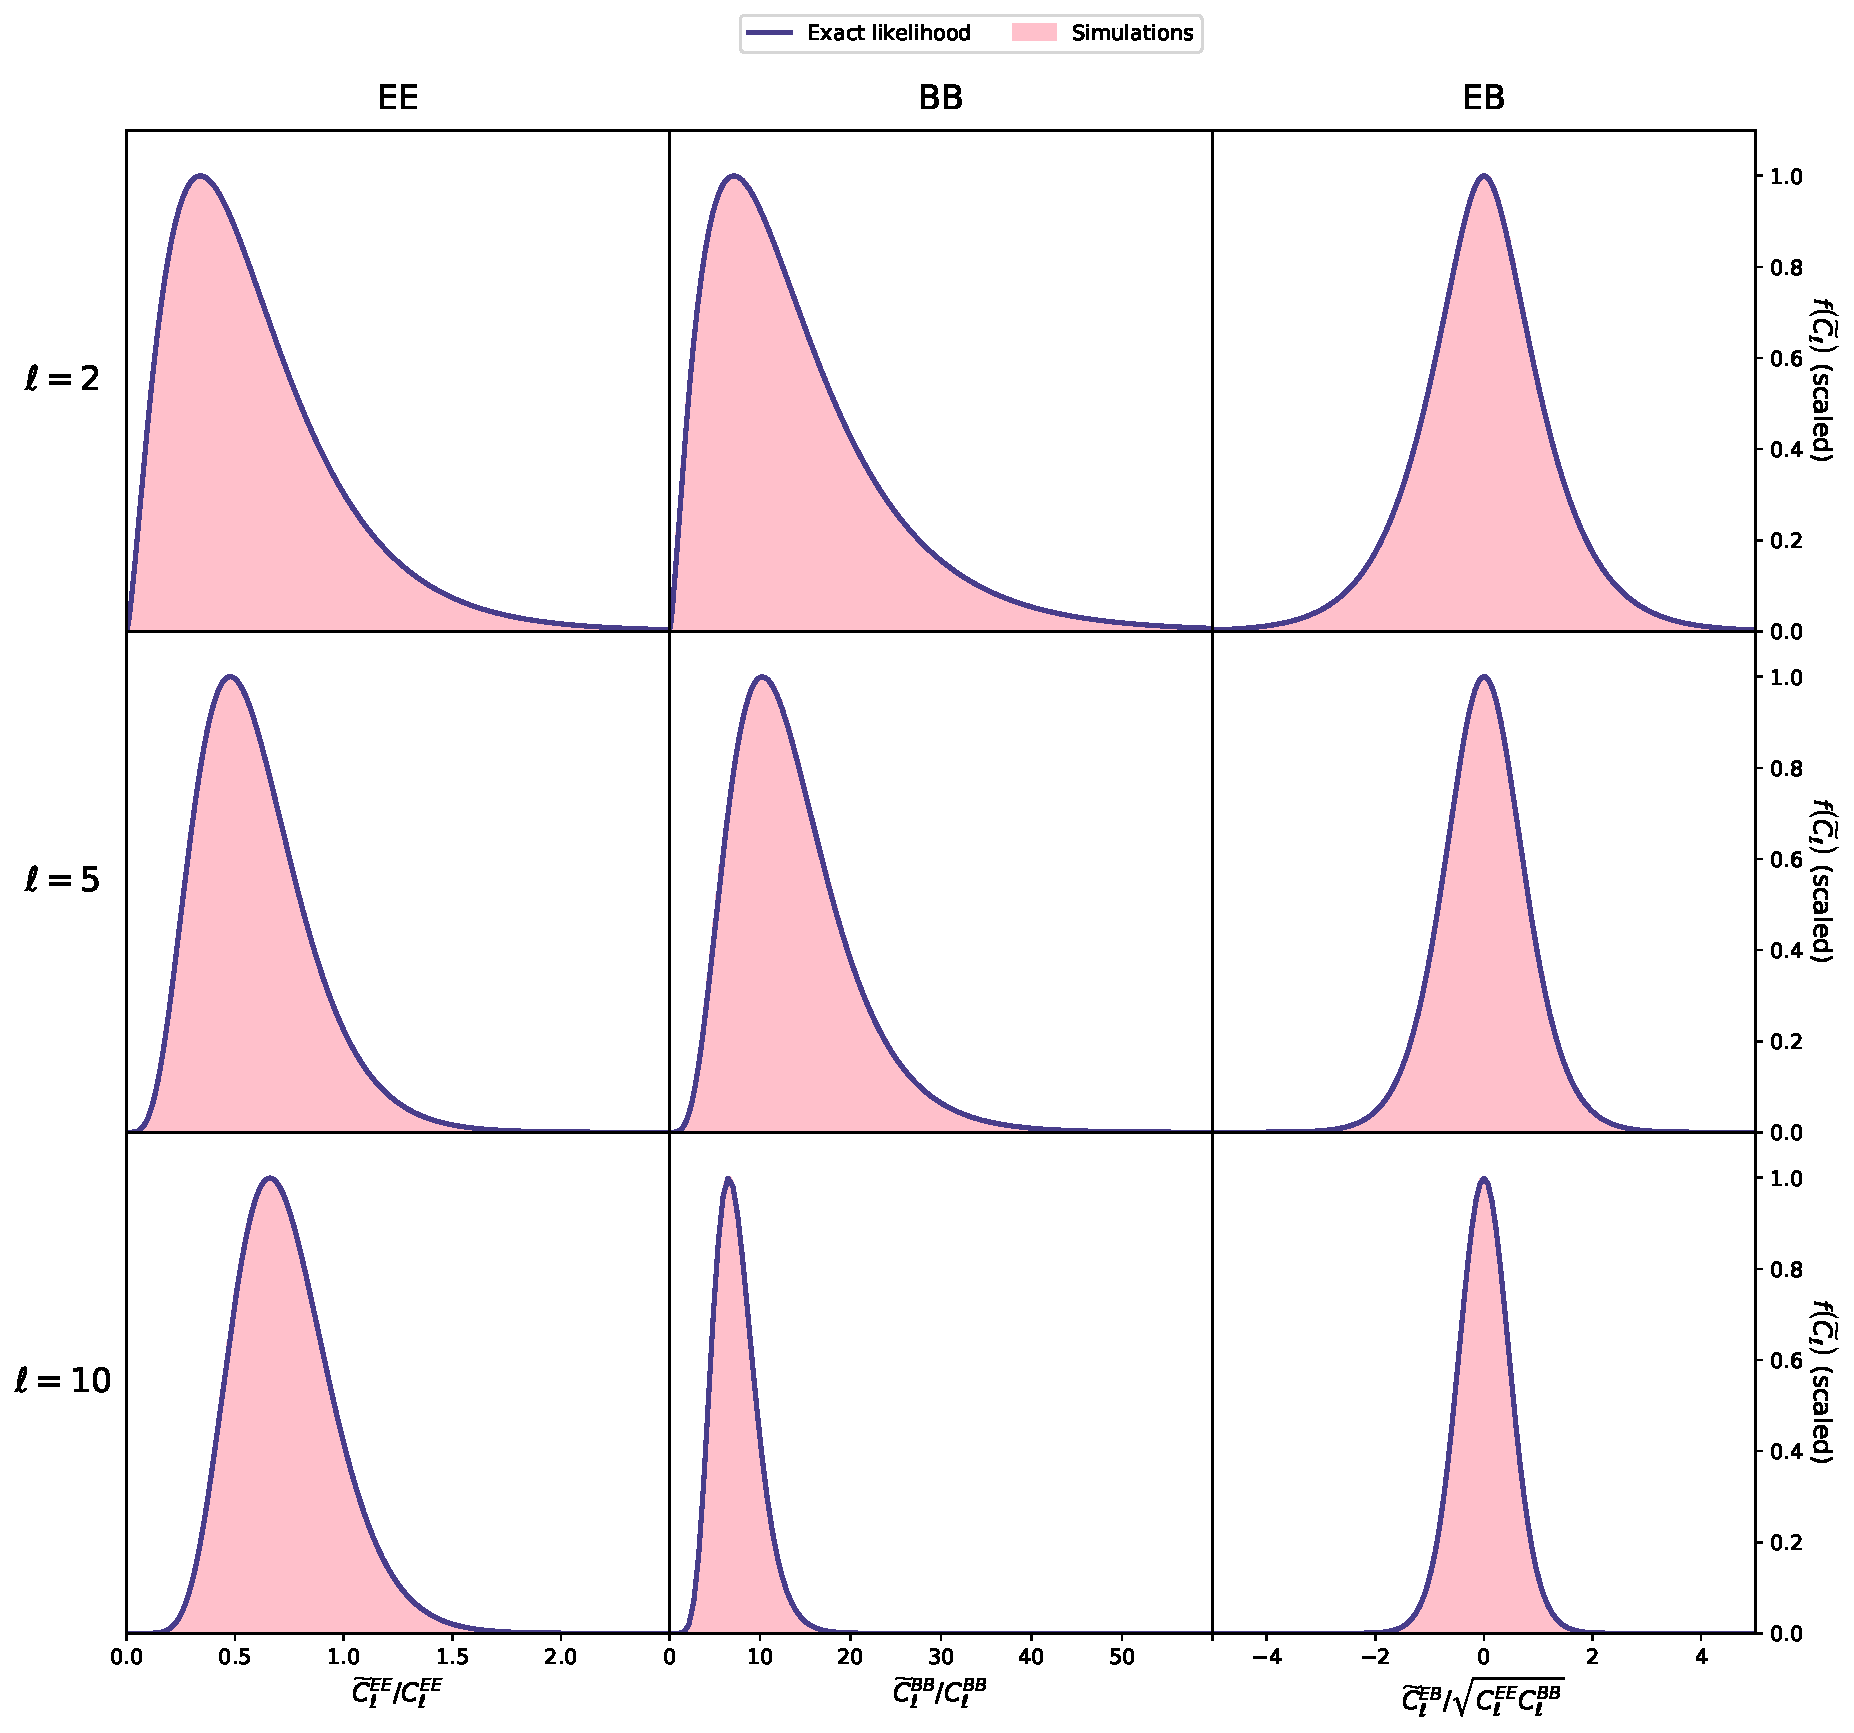
\includegraphics[width=\columnwidth]{marg_plots}
\caption{The marginal distributions of $\widetilde{C}_\ell^{EE}$, $\widetilde{C}_\ell^{BB}$ and $\widetilde{C}_\ell^{EB}$ for $\ell = 2$, 5 and 10, predicted by the exact likelihood for Gaussian fields presented in this chapter (blue curves) compared to those observed in the simulations (pink histograms). The maximum value of each curve has been rescaled to 1 for ease of comparison.}
\label{el_Fig:marginals}
\end{figure}

\autoref{el_Fig:marginals} shows the marginal distributions of $\widetilde{C}_\ell^{EE}$, $\widetilde{C}_\ell^{BB}$ and $\widetilde{C}_\ell^{EB}$ for each of $\ell = 2$, 5 and 10, to compare the prediction of the exact likelihood for Gaussian fields to the distributions observed in the simulations. Each histogram uses 300 bins. There is an excellent fit between the predicted and observed distribution, with no visible noise in the histograms due to the large number of events in each marginal distribution. The predicted likelihood exactly reproduces both the shape and amplitude of the observed distributions, including the considerable skewness in the auto-spectra. This skewness is reduced for higher multipoles, which is consistent with the full-sky behaviour of the likelihood.
Each auto-$\widetilde{C}_\ell$ in \autoref{el_Fig:marginals} has been scaled by the relevant theory $C_\ell$ used to generate both the theoretical likelihood and the simulations. In the case of the cross-spectrum $\widetilde{C}_\ell^{EB}$, there is no input $C_\ell^{EB}$ so instead $\sqrt{ C_\ell^{EE} C_\ell^{BB} }$ is used for the normalisation. This scaling allows us to observe that the $E$-mode power is reduced by the sky cut while the $B$-mode power is increased. This is a result of $E$--$B$ mixing: the $EE$ power spectrum is much larger in magnitude than the $BB$ power spectrum (by a factor $\sim 200$ at $\ell = 2$), meaning that the $E$--$B$ mixing induced by the mask leads to a relative increase in $B$-mode power at the expense of $E$-mode power.

\subsection{Correlation between spectra}

As well as exactly reproducing marginal distributions, the exact likelihood naturally describes correlations both between multipoles of the same spectrum and between spectra, for Gaussian fields. As described in \autoref{el_Sec:examples}, we formed the three-dimensional joint likelihood of $\widetilde{C}_\ell^{EE}$, $\widetilde{C}_\ell^{BB}$ and $\widetilde{C}_\ell^{EB}$ for $\ell = 2$. We formed the corresponding simulated distribution by binning events in three dimensions, using 100 bins in each dimension. We then integrated the exact likelihood over the volume of each histogram bin to allow for comparison between theory and simulations. Figures \ref{el_Fig:2D_EEBB}--\ref{el_Fig:2D_BBEB} show two-dimensional slices of this three-dimensional likelihood. Each slice corresponds to fixing a single histogram bin in one dimension and shows all bins in the other two dimensions. The exact likelihood appears to accurately match the observed distributions in all six slices to within pixel noise that arises from the finite number of realisations in the simulations. The right-hand panel for each slice shows the logarithmic fractional residual, defined as
\begin{equation}
    r = \log_{10} \left(
    \frac{\big\lvert
    \text{sampled density from simulations}
    - \text{density from exact likelihood}
    \big\rvert}{\text{density from exact likelihood}}
    \right).
    \label{el_Eqn:resid_def}
\end{equation}
Bins with no sampled events have $r = 0$ and appear as white in Figures \ref{el_Fig:2D_EEBB}--\ref{el_Fig:2D_BBEB}. These areas were not explicitly excluded, but their probability is very low (albeit non-zero). No clear evidence of structure is otherwise seen in these residuals, indicating that these bins contain only noise. This is mostly at the level of $r \approx -4$ to $-2$, except for a small number of outlying bins whose probability density is so low that the expected number of events in each bin from the 276~million simulations is significantly less than 1, leading to fractional residual values up to $r \approx 2$ in those bins in which an event was observed.

\begin{figure}
    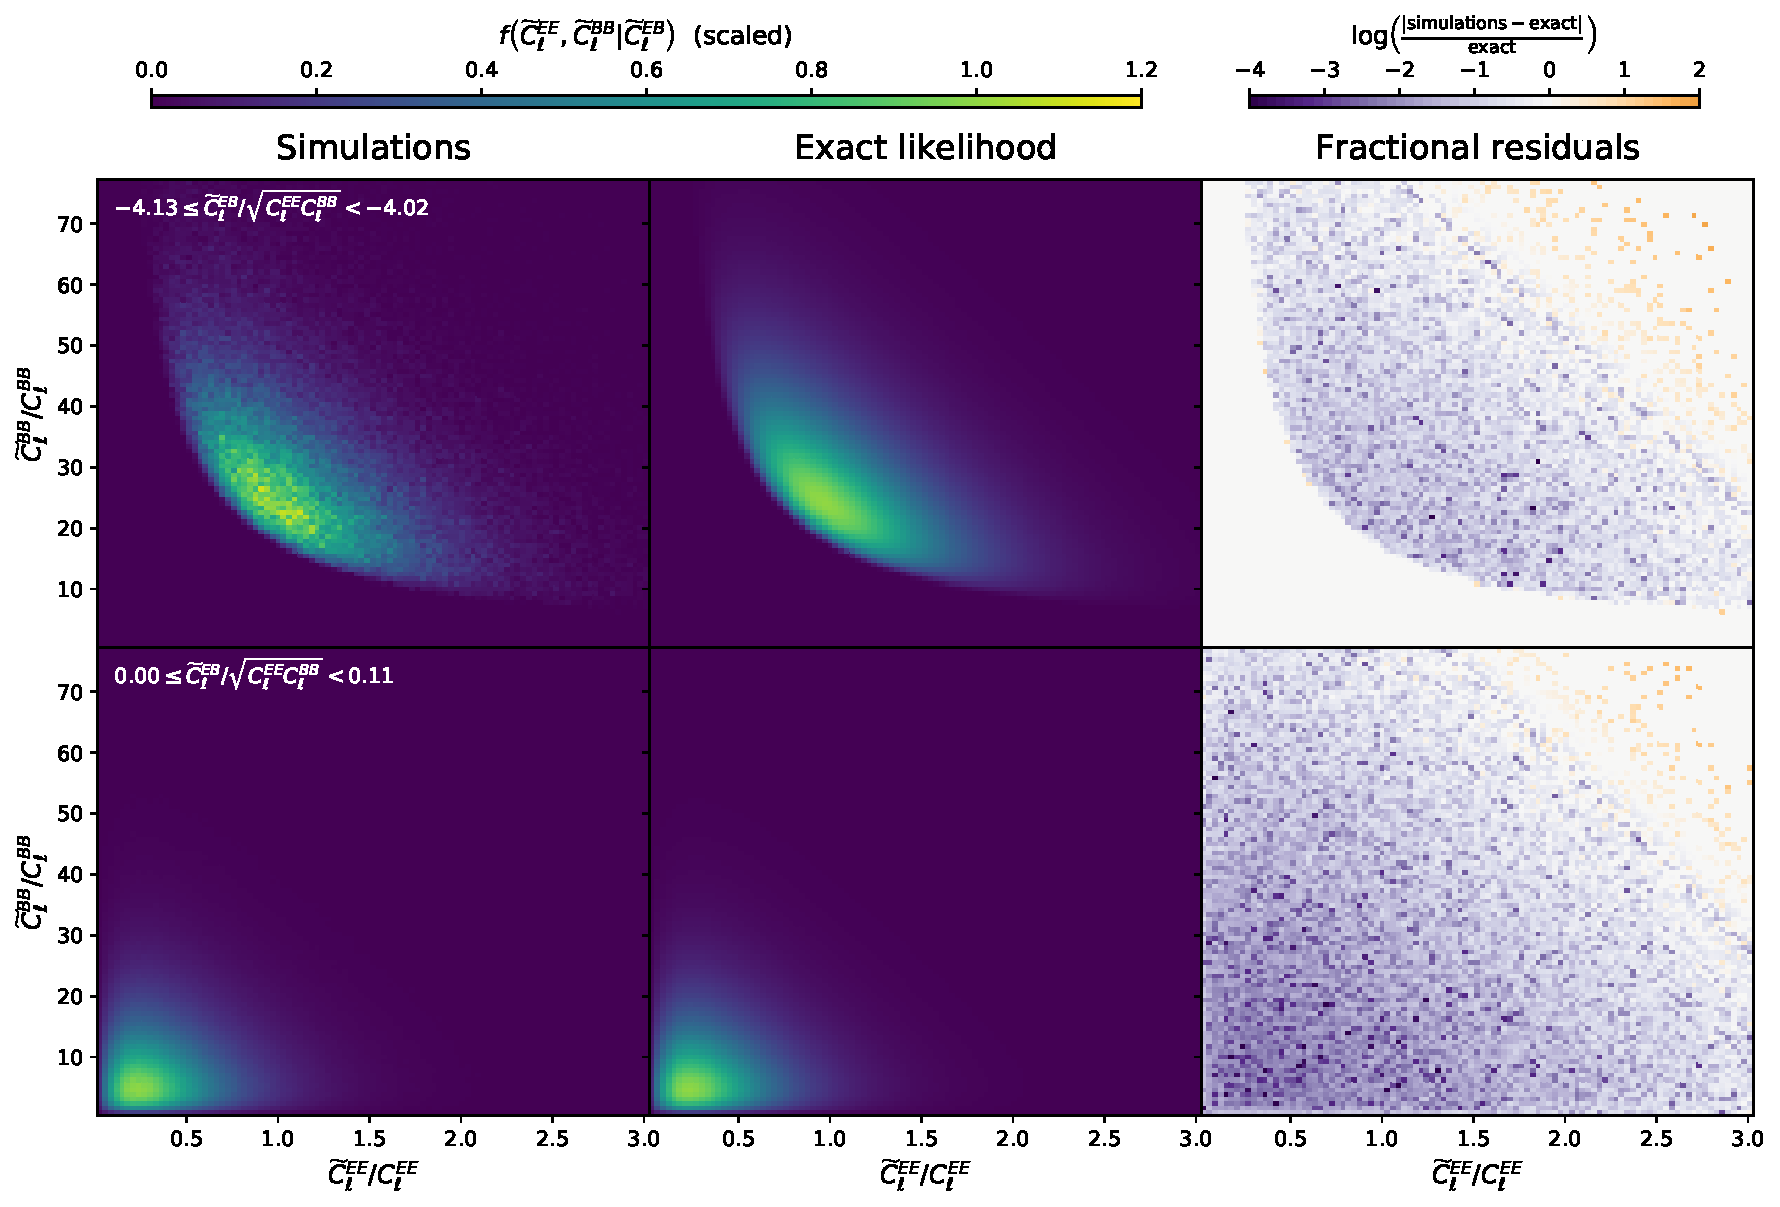
\includegraphics[width=\columnwidth]{2D_EEBB}
    \caption{Two different slices of the joint $\widetilde{C}_\ell^{EE}$--$\widetilde{C}_\ell^{BB}$ distribution for $\ell = 2$, each for one fixed bin of $\widetilde{C}_\ell^{EB}$. The top row is the slice corresponding to $-4.13~\leq~\widetilde{C}_\ell^{EB} / \sqrt{ C_\ell^{EE} C_\ell^{BB} } < -4.02$ while the bottom row corresponds to $0.00~\leq~\widetilde{C}_\ell^{EB} / \sqrt{ C_\ell^{EE} C_\ell^{BB} } < 0.11$. The left panel in each row is the distribution observed from simulations, while the centre panel is the distribution predicted by the exact likelihood for Gaussian fields. The same colour scale is used for the left and centre panels within each row and has been chosen such that the exact likelihood in each slice runs between 0 and 1. The right panels show logarithmic fractional residuals, as defined in Equation \eqref{el_Eqn:resid_def}, and contain only noise due to the finite number of realisations.}
    \label{el_Fig:2D_EEBB}
\end{figure}
\begin{figure}
    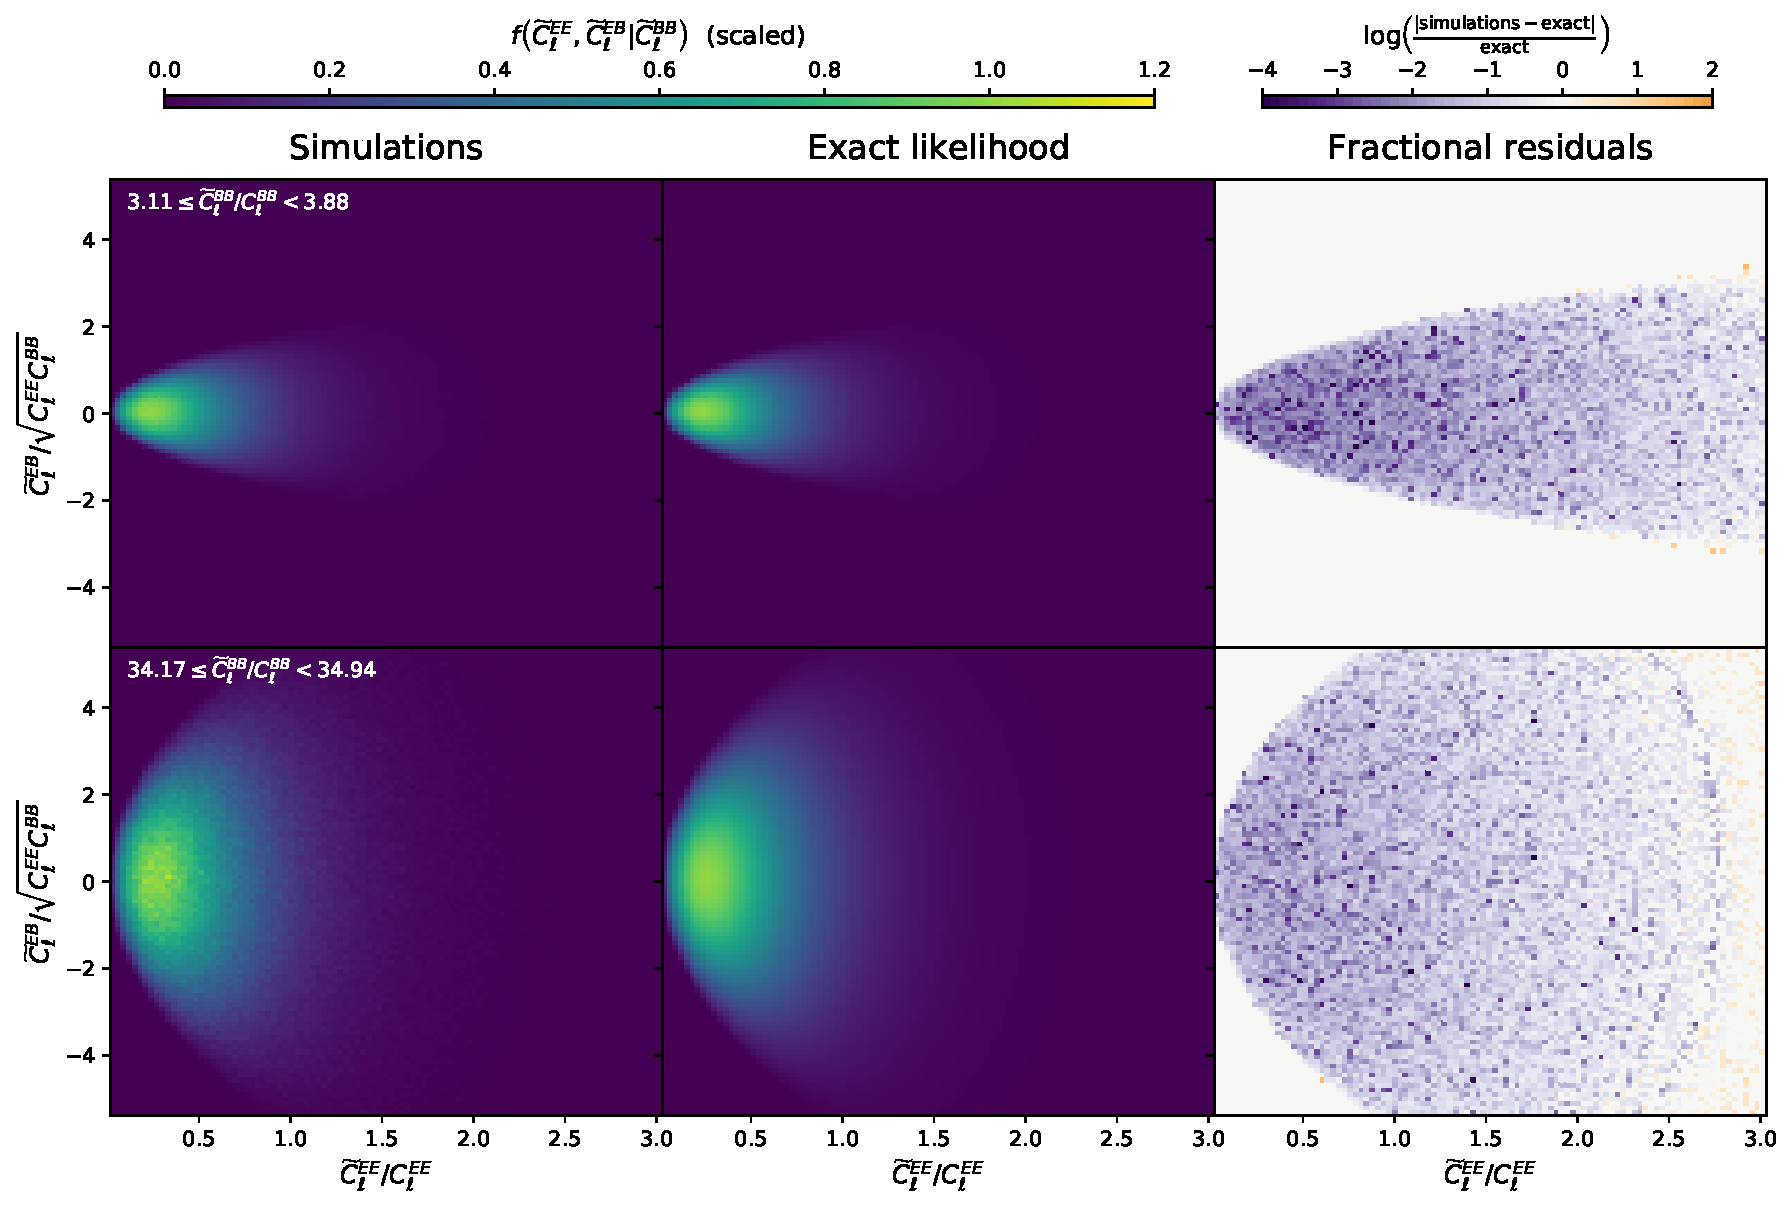
\includegraphics[width=\columnwidth]{2D_EEEB}
    \caption{As \autoref{el_Fig:2D_EEBB}, but for the $\widetilde{C}_\ell^{EE}$--$\widetilde{C}_\ell^{EB}$ distribution at fixed values of $\widetilde{C}_\ell^{BB}$. The top row corresponds to $3.11~\leq~\widetilde{C}_\ell^{BB} / C_\ell^{BB} < 3.88$ and the bottom row to $34.17~\leq~\widetilde{C}_\ell^{BB} / C_\ell^{BB} < 34.94$.}
\end{figure}
\begin{figure}
    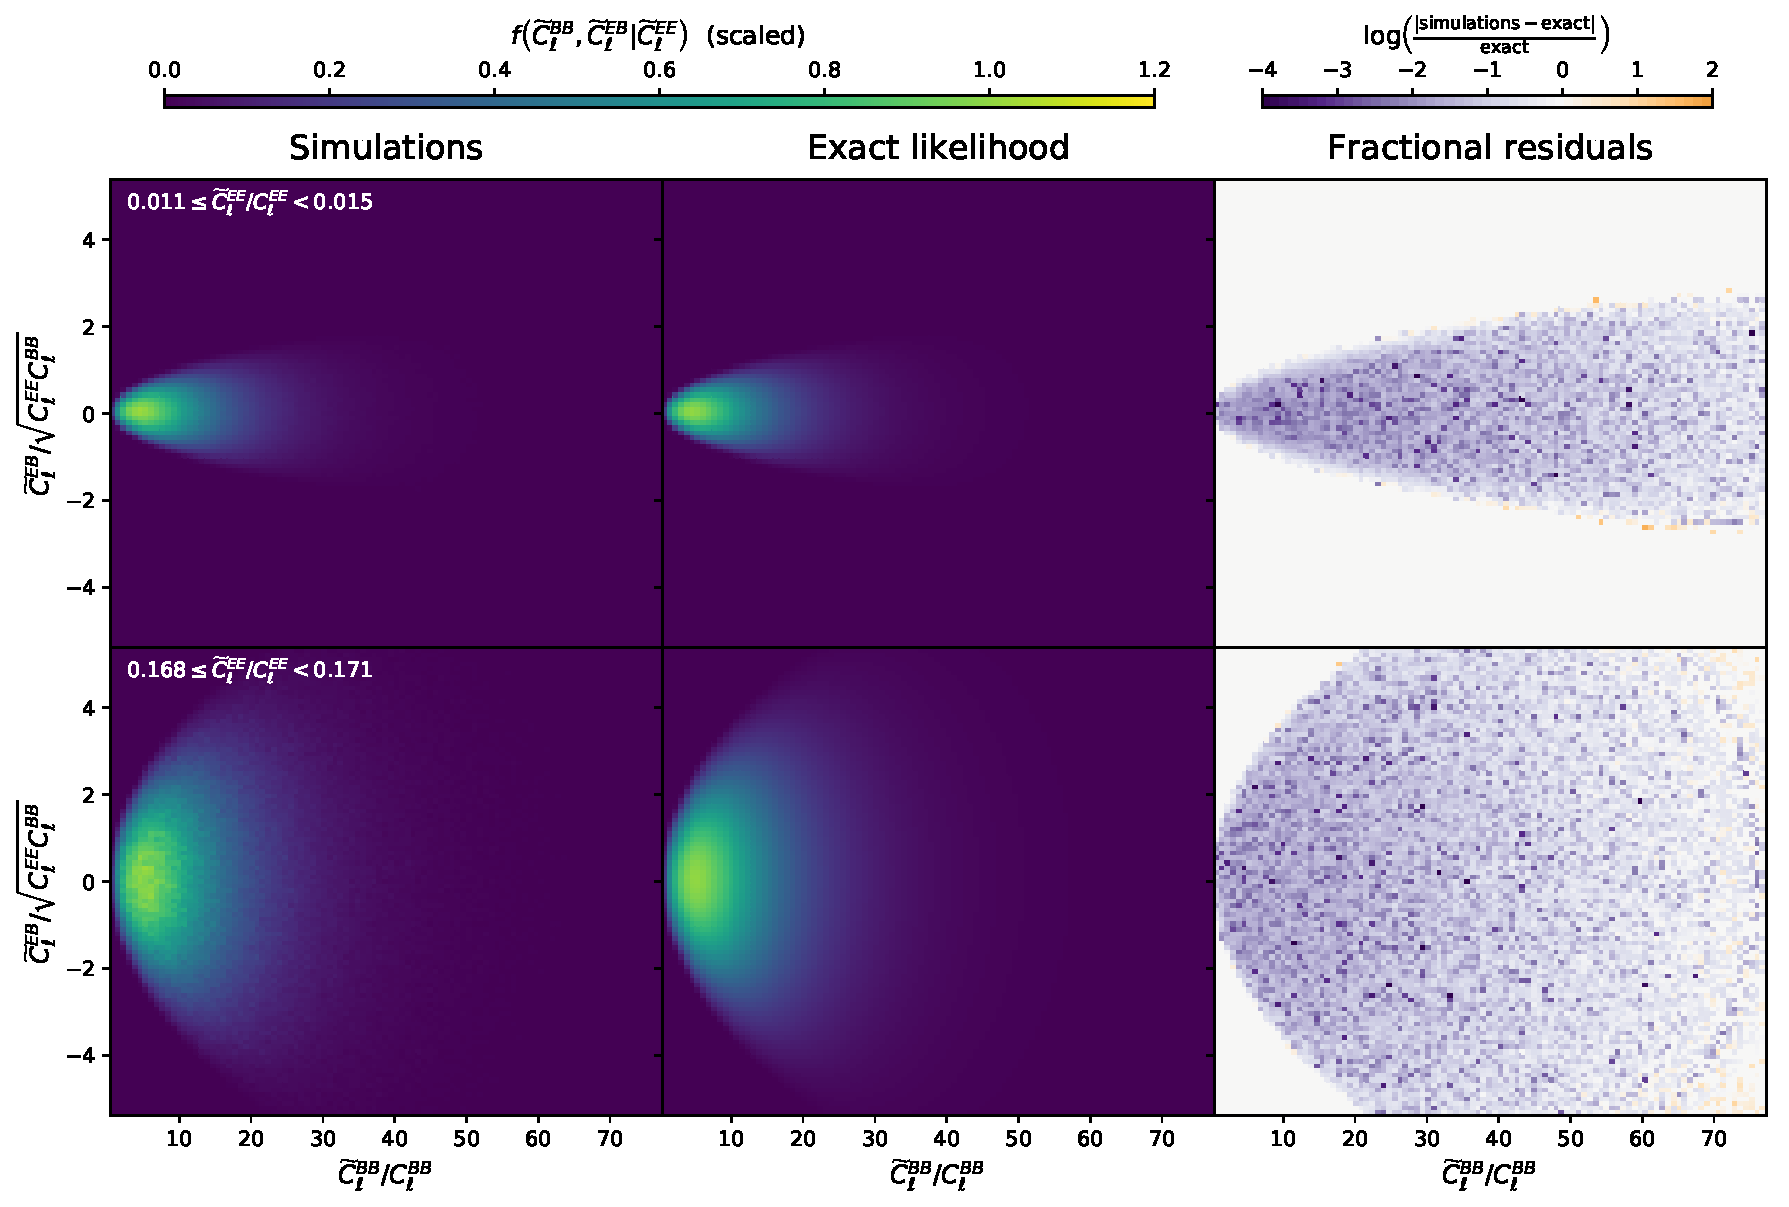
\includegraphics[width=\columnwidth]{2D_BBEB}
    \caption{As \autoref{el_Fig:2D_EEBB}, but for the $\widetilde{C}_\ell^{BB}$--$\widetilde{C}_\ell^{EB}$ distribution at fixed values of $\widetilde{C}_\ell^{EE}$. The top row corresponds to $0.011~\leq~\widetilde{C}_\ell^{EE} / C_\ell^{EE} < 0.015$ and the bottom row to $0.168~\leq~\widetilde{C}_\ell^{EE} / C_\ell^{EE} < 0.171$.}
    \label{el_Fig:2D_BBEB}
\end{figure}

\subsubsection{Comparison to approximation}

In this section, the exact likelihood is compared to a Wishart distribution with fitted parameters $\nu_\mathrm{eff}$ and $\mathbfss{W}_\ell^\mathrm{eff}$, as described in \autoref{el_Eqn:sec_approx}. This comparison is not included to advocate for the use of this approximation; on the contrary, the aim is to demonstrate the merits of using the exact likelihood for Gaussian fields. For this reason, it is not a concern whether appropriate values of $\nu_\mathrm{eff}$ and $\mathbfss{W}_\ell^\mathrm{eff}$ can be obtained in practice. We simultaneously fitted the three marginals of a $p=2$ Wishart distribution to the exact marginals, and obtained the following best-fitting values:
\begin{equation}
    \frac{\nu_\mathrm{eff}}{2 \ell + 1} = 1.0; \quad \quad
    \mathbfss{W}_\ell^\mathrm{eff} = \frac{1}{2 \ell + 1}
    \begin{pmatrix}
    0.59 C_\ell^{EE} & 0 \\
    0 & 14 C_\ell^{BB}
    \end{pmatrix}.
    \label{el_Eqn:wish_params}
\end{equation}

\begin{figure}
    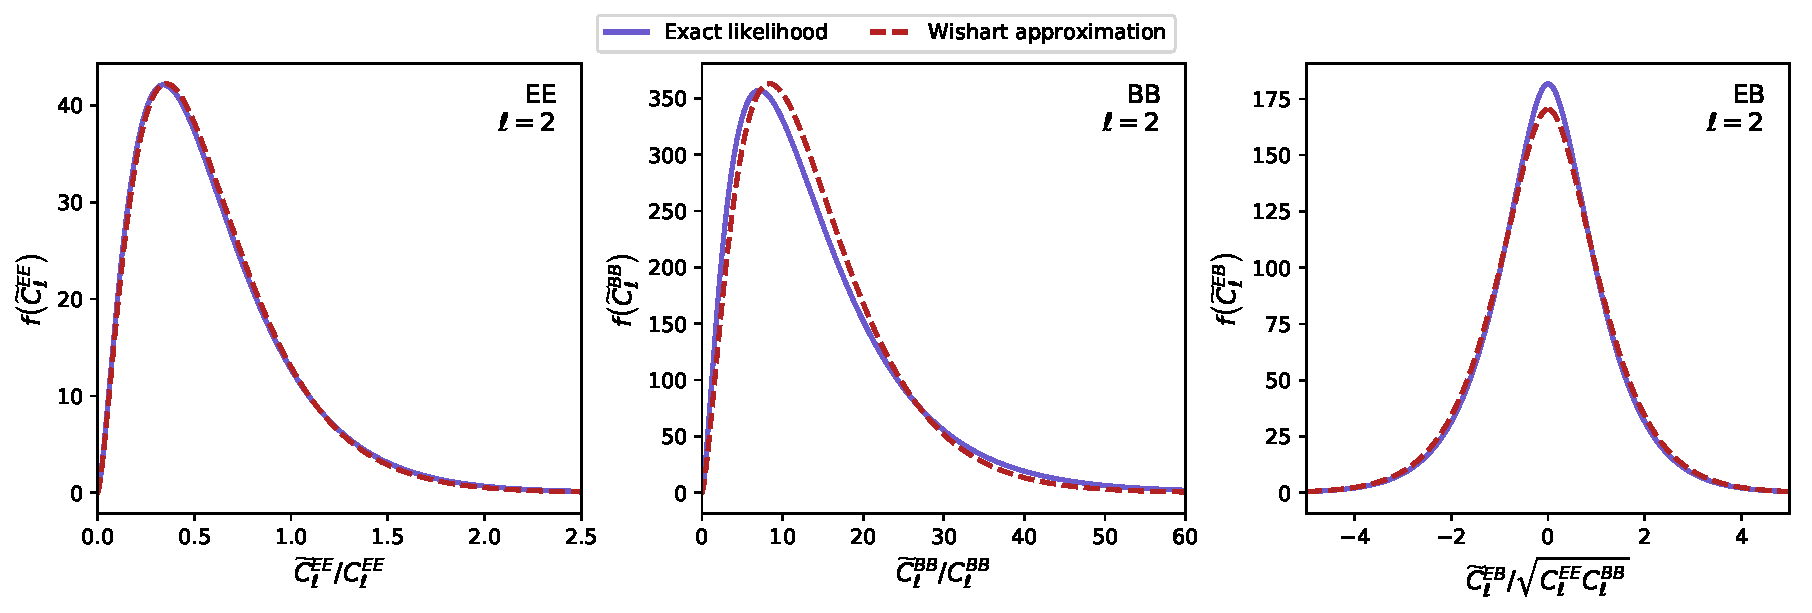
\includegraphics[width=\columnwidth]{marg_vs_approx}
    \caption{Marginal distributions based on the Wishart approximation with best-fitting parameters given in Equation \eqref{el_Eqn:wish_params} (dashed red curves) compared to the exact likelihood for Gaussian fields (solid blue curves).}
    \label{el_Fig:marg_vs_approx}
\end{figure}

There is no reason to expect that these values would also be the best-fitting values for a different $\ell$ or for a different input cosmology, and they would certainly be different for another mask. The resulting marginal distributions are shown in \autoref{el_Fig:marg_vs_approx}, where the simulated histogram is omitted for clarity. The fit is almost perfect for $\widetilde{C}_\ell^{EE}$, indicating that this marginal distribution closely follows a gamma distribution as in the full-sky case. There is slightly more deviation for $\widetilde{C}_\ell^{BB}$ and $\widetilde{C}_\ell^{EB}$.

\begin{figure}
    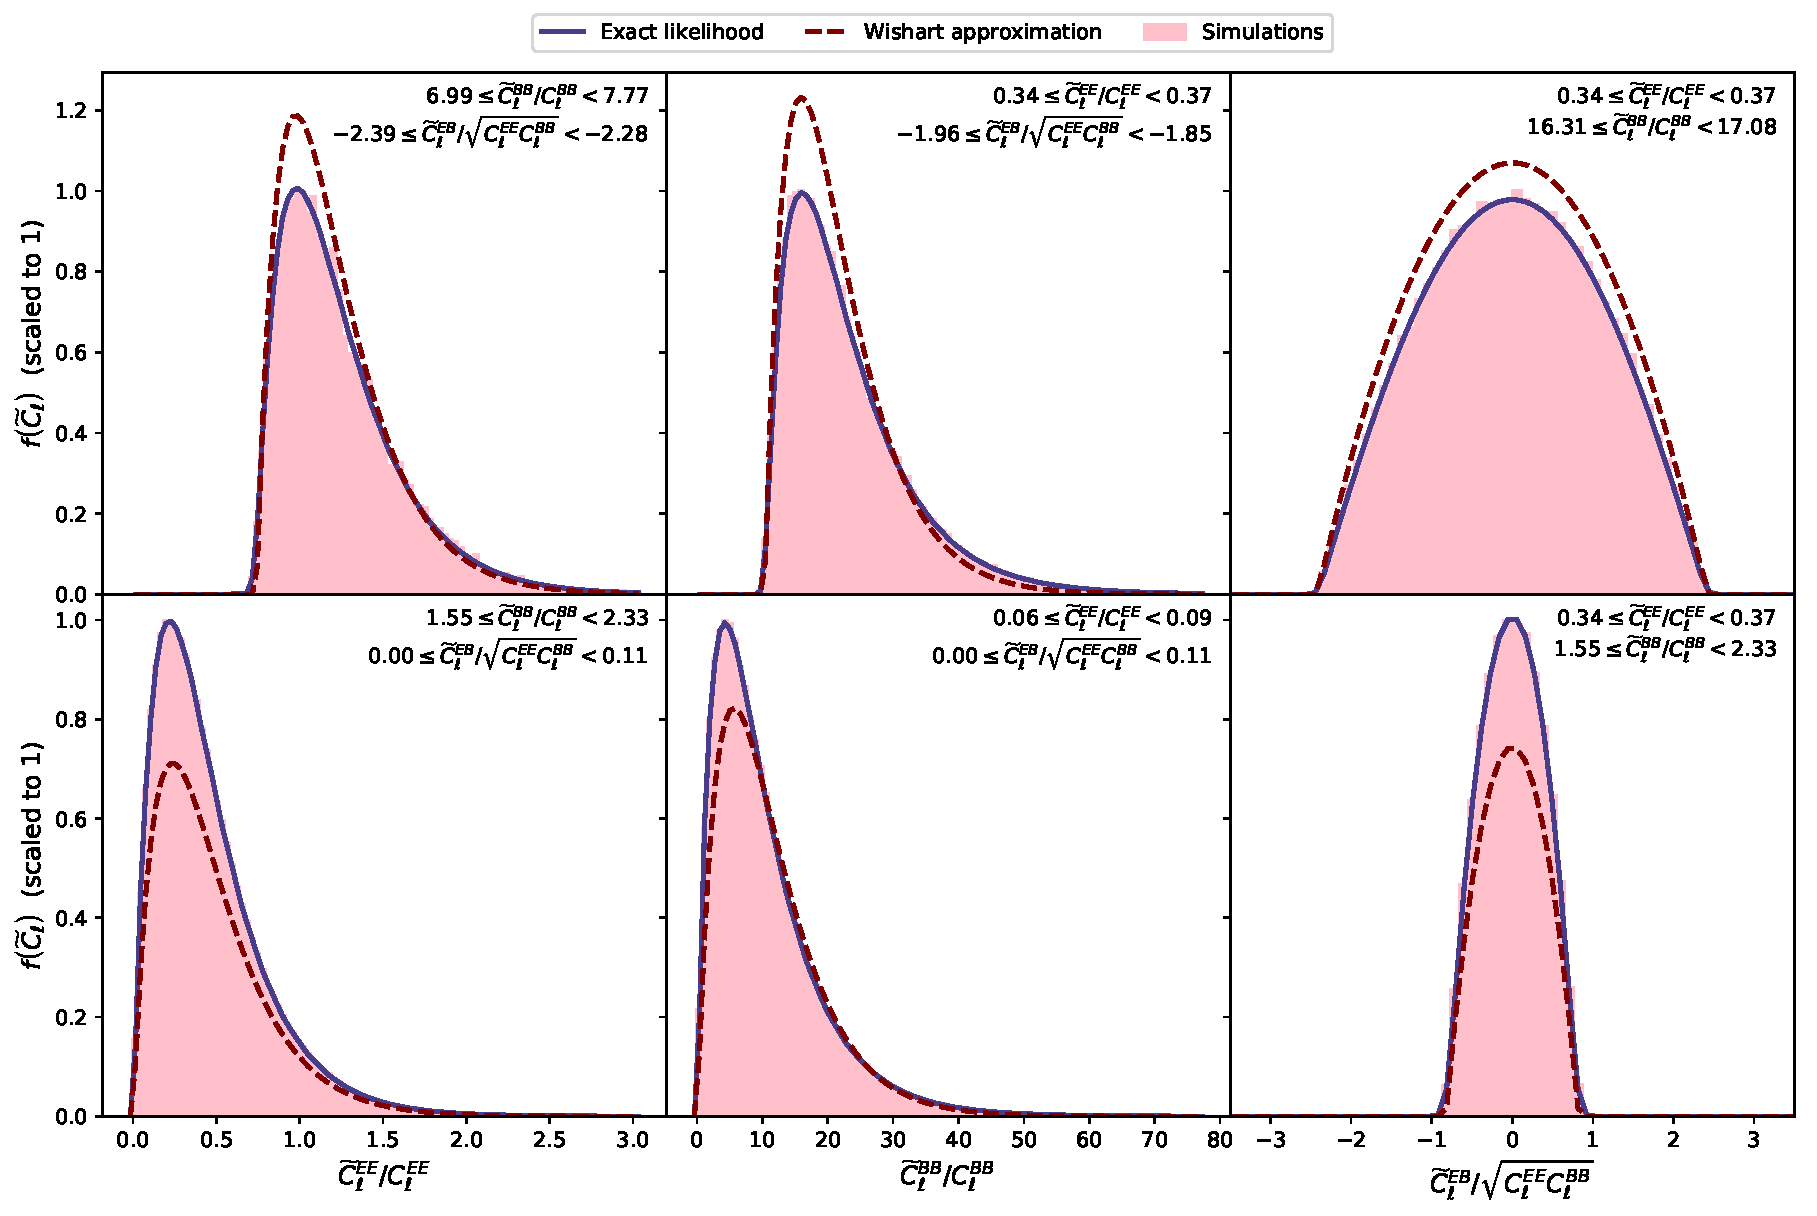
\includegraphics[width=\columnwidth]{1dslices_vs_approx}
    \caption{One-dimensional slices of the joint distribution of $\widetilde{C}_\ell^{EE}$, $\widetilde{C}_\ell^{BB}$ and $\widetilde{C}_\ell^{EB}$ for $\ell = 2$. In each slice, two of the values are fixed while the third is allowed to vary.}
    \label{el_Fig:1dslices_vs_approx}
\end{figure}

\begin{figure}
    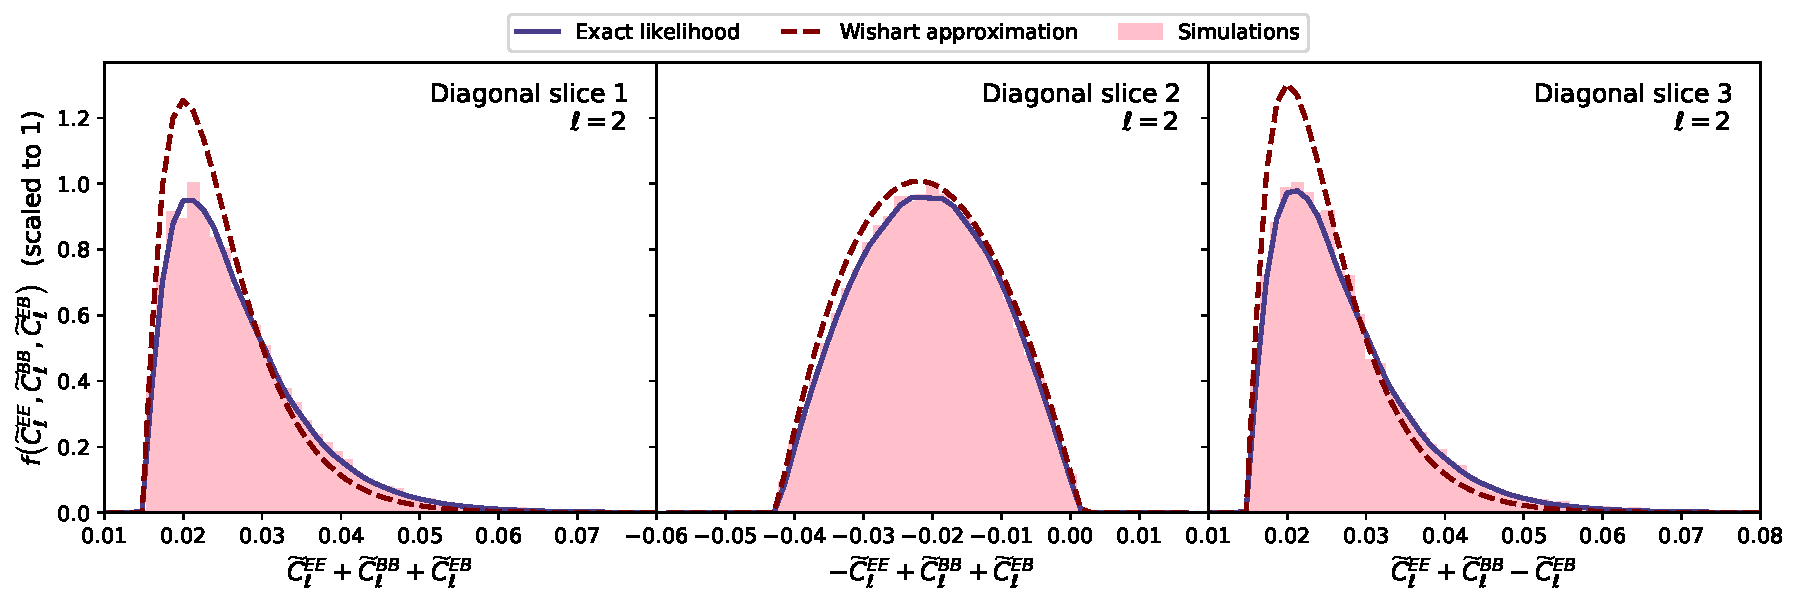
\includegraphics[width=\columnwidth]{diag_vs_approx}
    \caption{As \autoref{el_Fig:1dslices_vs_approx} but for slices taken in three diagonal directions, each corresponding to a linear combination of the three pseudo-$C_\ell$s.}
    \label{el_Fig:diag_vs_approx}
\end{figure}

We integrated the Wishart probability density over each histogram bin in three-dimensional space, as with the exact likelihood for Gaussian fields. \autoref{el_Fig:1dslices_vs_approx} shows one-dimensional slices through this three-dimensional likelihood. For each slice, two dimensions have been fixed at a single histogram bin, and the distribution across the third dimension is shown. While the marginal distributions suggest a near-exact fit for the Wishart approximation, the one-dimensional slices reveal that the approximation incorrectly distributes probability in some parts of the three-dimensional space relative to other parts. The exact likelihood for Gaussian fields, on the other hand, faithfully reproduces the observed distribution throughout. This is also seen in \autoref{el_Fig:diag_vs_approx}, which shows three one-dimensional slices in different diagonal directions across the three-dimensional space. In each of these slices, the Wishart approximation overestimates the probability density relative to the true distribution, implying that it must underestimate it in other parts of the distribution, given that the whole distribution is normalised to integrate to 1.

As well as failing to accurately reproduce the full distribution for a fixed $\ell$, the Wishart distribution cannot naturally be extended to include correlations between multipoles, whereas the exact likelihood automatically produces the full joint distribution between all multipoles of all power spectra measured on Gaussian fields. In some cases an approximation may work better over the joint distribution of many multipoles than for a single $\ell$ \citep{Hamimeche2008}, but the inverse can also be true \citep{Elsner2012}. In any case, the choice of approximation for the purposes of this comparison is unimportant: no approximation can completely match the exact distribution.


\section{Conclusions}
\label{el_Sec:conclusions}

This chapter has presented the exact joint likelihood of an arbitrary number of pseudo-$C_\ell$ estimates from correlated Gaussian fields, valid for both auto- and cross-power spectra and for any mask geometry. The likelihood---given in Equation \eqref{el_Eqn:joint_likelihood}---naturally models both intrinsic correlations between spin-0 and spin-2 fields, and correlations induced by a cut sky which result in the mixing between spherical harmonic coefficients. The pseudo-$a_{\ell m}$s follow a multivariate Gaussian distribution with covariance matrix elements given by Equations \eqref{el_Eqn:cov_re_re_general}--\eqref{el_Eqn:cov_re_im_general}. The exact joint likelihood for QML power spectrum estimates from Gaussian fields has also been presented, in Equation \eqref{el_Eqn:qml_distribution}. An accurate likelihood function is an essential companion to any estimator for unbiased cosmological inference, but until now a complete likelihood for either the pseudo-$C_\ell$ or QML estimator on an arbitrary sky has not been known.

Sections \ref{el_Sec:examples} and \ref{el_Sec:results} showed how the exact likelihood can be applied to observations of the polarisation of the Cosmic Microwave Background. This is especially relevant given current and future experiments aimed at detecting primordial $B$-modes, which require exquisite control of all possible sources of systematic bias. One such source of bias is an inexact likelihood function, so knowledge of the exact likelihood could play an important role in extracting cosmological information from polarisation measurements in an unbiased manner. In particular, it exactly models the leakage of $E$-mode power into the much smaller $B$-mode signal. This likelihood also extends naturally to include correlations between temperature anisotropy and polarisation, including cross-correlations between any number of detectors, where each observed temperature or polarisation field may have its own mask. It does not account for weak gravitational lensing of the CMB, which breaks the assumption of Gaussianity at higher multipoles.

The exact likelihood for Gaussian fields could also be extremely useful for weak lensing observations. It will perhaps be most valuable at relatively low multipoles, as this is the regime where the common assumption of a Gaussian likelihood for power spectrum estimates is least applicable due to the considerable skewness in the true likelihood \citep[e.g.][]{Sellentin2018a}. These low multipoles correspond to large physical scales, for which it is an excellent approximation to describe the spin-2 cosmic shear field as a Gaussian field. At higher multipoles there will be significant deviations from Gaussianity, so this likelihood cannot be considered exact on small scales. The likelihood naturally extends to describe the full distribution of auto- and cross-power spectra between an arbitrary number of redshift bins, each with its own mask. It is thus well suited for extracting robust cosmological constraints from tomographic galaxy clustering and weak lensing shear power spectrum measurements in multiple redshift bins, such as those from \Euclid{}.

Use of the exact pseudo-$C_\ell$ likelihood for Gaussian fields is likely to be competitive in terms of speed when considering a small number of bandpower estimates. Its main strength compared to an exact pixel-based likelihood is that for a single power estimate the pseudo-$C_\ell$ likelihood requires the determinant evaluation of a matrix of size $\sim \ell$ compared to $\sim \ell^2$ for a pixel-based method. This means that it may be evaluated at much higher $\ell$ than is possible for a pixel-based method. However, once many power estimates are considered the scaling is less competitive. The pixel-based method would offer all additional multipoles $\ell' < \ell$ without significant additional computational cost, while the exact pseudo-$C_\ell$ likelihood for Gaussian fields scales as $\sim k^N$, where $N$ is the number of (band)power estimates and $k \sim 200$. The cost is driven by the need to evaluate the characteristic function in Equation \eqref{el_Eqn:joint_cf} for every value of the vector $\mathbfit{t}$. The range of $\mathbfit{t}$ must cover a wide enough space for the integral in the likelihood expression to converge, while at a sufficiently high resolution so that its curvature is accurately represented. Each point in $\mathbfit{t}$-space carries its own determinant or eigenvalue calculation (which is not the case for a single power estimate, due to the simple scaling of the determinant of a single matrix).
% Use of the exact likelihood for Gaussian fields is therefore only recommended in the case of a small number of bandpower estimates, and are exploring alternative (necessarily approximate) approaches for the joint distribution of many power estimates, including the use of a copula with the exact marginal distributions.
Use of the exact likelihood for Gaussian fields is therefore only recommended in the case of a very small number of bandpower estimates, and alternative (necessarily approximate) approaches for the joint distribution of many power estimates should be explored. One possibility is the use of a copula with the exact marginal distributions.
Copula methods have previously been described in a cosmological context, but only with approximate marginal distributions \citep{Benabed2009, Sato2010, Sato2011}. Alternative approaches previously explored in the literature include approximate extensions to the Wishart distribution to model correlations between multipoles \citep{Hamimeche2008, Mangilli2015}. Computational limitations in the likelihood calculation may also be mitigated to some extent by potential speed increases at other levels in the inference process such as neural net-assisted sampling \citep{Manrique-Yus2020}.

Despite the limitations of its direct use, knowledge of the exact pseudo-$C_\ell$ and QML likelihood for Gaussian fields is extremely useful as a starting point and testing benchmark for developing fast, accurate approximations. It is used for this purpose in the work presented in \autoref{chap:gauss_like}. A common approach to a total likelihood, particularly for CMB observations \citep[e.g.][]{Planck2018V} is to use an exact pixel-based likelihood at low multipoles and to switch to an approximate Gaussian power spectrum likelihood for higher multipoles, at the point at which a pixel-based likelihood becomes computationally unfeasible (at $\ell = 29$ in the case of \Planck{}, while for weak lensing analyses with many redshift bins an exact pixel-based method may not be feasible at all). Methods derived from this exact likelihood for Gaussian fields may fill an important niche between these two regimes, allowing the use of an exact or near-exact likelihood up to higher multipoles than is currently possible. This may be a powerful tool for interpreting future observations, given the increased statistical precision that they will offer. This likelihood also has the advantage that it can naturally describe the cross-correlation power spectrum measured between two different maps, in contrast to exact pixel-based methods which are not readily adapted to extracting just the cross-correlation information. Considering only cross-spectra in this way makes the cosmological analysis insensitive to the details of the noise bias, which will be especially relevant for cosmic shear observations, for which shape noise is an important and uncertain factor.


% % Uncomment to build alone without subfiles:
% \printbibliography[heading=bibintoc]
% \end{document}


% Sufficiency of a Gaussian likelihood for weak lensing power spectra

% % Uncomment to build this alone without subfiles:
% % (also stuff at bottom)
% \documentclass{scrbook}
% % \documentclass[draft]{scrbook} % use this to mark overfull hboxes in black
% % Koma script document options
\KOMAoption{paper}{a4}
\KOMAoption{fontsize}{11pt}
\KOMAoption{parskip}{half-} % paragraph spacing
% \KOMAoption{numbers}{enddot} % dot after section number
\KOMAoption{cleardoublepage}{plain} % include page numbers on blank pages
\KOMAoption{chapterprefix}{true} % 'Chapter' before number

% Packages
\usepackage{amsmath} % Gives \text command inside maths blocks
\usepackage{amssymb} % Various maths symbols
\usepackage{array} % Table formatting
\usepackage{bm} % Bold maths including Greek
\usepackage[format=plain]{caption} % Font sizing and alignment in captions
\usepackage{enumitem} % Allows numbering like 1.1 in ordered lists
% \usepackage{float} % Allows H placement of floats
\usepackage{graphicx}
\usepackage[hidelinks]{hyperref} % Hyperlinks without looking like it
% \usepackage{longtable} % Multi-page tables
% \usepackage{multicol} % For columns in text (not tables)
\usepackage{multirow} % For tables
\usepackage{neuralnetwork} % Neural net diagram
\usepackage{pdflscape} % Gives landscape environment
% \usepackage{scrlayer-scrpage} % To move page numbers
\usepackage{tabularx}
\usepackage{textcomp} % Added to fix \textasciiacute error on laptop
% \usepackage{tikz} % Diagrams (used for neural network example)
% \usepackage[pagenumberwidth=3em]{tocbasic}
% \usepackage{tocstyle} % ToC styling
\usepackage{upgreek} % Non-italic greek letters
\usepackage{xpatch} % Biblatex customisation

\usepackage[a4paper, inner=40mm, outer=15mm, top=30mm, bottom=30mm,footskip=15mm, headsep=15mm]{geometry}
% \usepackage[a4paper, inner=40mm, outer=30mm, top=50mm, bottom=50mm,footskip=20mm, headsep=20mm]{geometry} % footskip is space between footer (i.e. page number) and bottom of text
% min allowed is inner 40 mm, others 15 mm

\pagestyle{plain} % no header for front matter, overridden at end of front matter

% Caption setup
% \tablecaptionabove
\captionsetup[table]{labelsep=space}
% \captionsetup[table]{labelsep=space, skip=50pt, position=top}
\captionsetup[figure]{labelsep=space} % labelsep prevents dot followed by colon in captions

% Line spacing
\usepackage{setspace}
% \setstretch{1.4} % strangely this is > \onehalfspacing but < \doublespacing
\onehalfspacing
% \doublespacing

\raggedbottom % prevent huge spaces between paragraphs

% % % % % % % % % % % % % % % % % % % % % % % % %
% Font setup
% \usepackage{mathpazo} % Covers maths mode too
\usepackage[sc]{mathpazo} % Covers maths mode too, sc enables small caps
% \usepackage{palatino}
\usepackage[T1]{fontenc} % 8-bit font encoding
\addtokomafont{disposition}{\rmfamily} % Use serif throughout
% % % % % % % % % % % % % % % % % % % % % % % % %

% % % % % % % % % % % % % % % % % % % % % % % % %
% Section formatting setup
% \RedeclareSectionCommand[beforeskip=0pt]{chapter}
\RedeclareSectionCommand[beforeskip=0pt, innerskip=0pt]{chapter}
\RedeclareSectionCommand[beforeskip=10pt]{subsubsection}
\RedeclareSectionCommand[afterskip=1pt]{subsubsection}
% \setcounter{secnumdepth}{\subsubsectionnumdepth} % number up to subsubsections

% No dot after chapter number (https://tex.stackexchange.com/a/484727)
\renewcommand*{\chapterformat}{%
  \mbox{\chapappifchapterprefix{\nobreakspace}\thechapter
  \IfUsePrefixLine{}{\enskip}}%
}

% In the running header, separate chapter number and name with em dash
\renewcommand*{\chaptermarkformat}{%
\chapapp~\thechapter~---~}

% Create subsubsubsection below subsubsection but above paragraph, following https://tex.stackexchange.com/a/356574

\DeclareNewSectionCommand[
  style=section,
  counterwithin=subsubsection,
  afterskip=1pt,
  beforeskip=10pt,
  % afterskip=1.5ex plus .2ex,
  % beforeskip=3.25ex plus 1ex minus .2ex,
  % afterindent=false,
  level=\paragraphnumdepth,
  tocindent=10em,
  tocnumwidth=5em
]{subsubsubsection}
\setcounter{secnumdepth}{\subsubsubsectionnumdepth}
% \setcounter{tocdepth}{\subparagraphtocdepth}
\setcounter{tocdepth}{\subsubsubsectionnumdepth}

\RedeclareSectionCommands[
  level=\numexpr\subsubsubsectionnumdepth+1\relax,
  toclevel=\numexpr\subsubsubsectiontocdepth+1\relax,
  increaselevel,
]{paragraph,subparagraph}
\RedeclareSectionCommand[
  counterwithin=subsubsubsection,
  tocindent=12em,
  tocnumwidth=6em,
  beforeskip=10pt,
  afterskip=1pt, % line break after paragraph title
]{paragraph}
\RedeclareSectionCommand[
  tocindent=14em,
  tocnumwidth=7em,
  beforeskip=0pt
]{subparagraph}
% % % % % % % % % % % % % % % % % % % % % % % % %

% Autoref capitalisation
\def\chapterautorefname{Chapter}
\def\sectionautorefname{Section}
\def\subsectionautorefname{Section}
\def\subsubsectionautorefname{Section}

% % % % % % % % % % % % % % % % % % % % % % % % %
% Bibliography setup
\usepackage[backend=biber,
    % style=authoryear,
    style=authoryear-comp, % Don't repeat same author(s) in multiple citations
    giveninits=true,
    useprefix=true, % 'van der' etc.
    url=false,
    doi=false,
    isbn=false,
    eprint=false,
    uniquename=false, % Don't add initials in citation to disambiguate between authors with the same surname
    uniquelist=false, % Don't disambiguate in citation between different 'et al.' teams
    maxbibnames=10,
    minbibnames=10,
    maxcitenames=3,%  # 2,
    natbib, % Gives citep and citet commands
    labelalpha=true, % Use an 'alpha' label for each bib entry
    maxalphanames=1, % Use first author as the alpha label
    sorting=anyvt, % Sort by alpha (first author) then year
    block=par, % New line between 'blocks' of the bib entry
    dashed=false, % Reprint author list for each publication in bibliography
    sortcites=false % Show citations in the order supplied
]{biblatex}

% Citation/reference parameters
\renewcommand*{\nameyeardelim}{\addspace} % Space between author and year rather than comma
\renewcommand*{\finalnamedelim}{\addspace\&\addspace} % Ampersand rather than 'and'
\xpatchbibmacro{name:andothers}{{\finalandcomma}}{\addspace}{}{} % Space before 'et al.' rather than comma

% Citation-specific parameters
\DeclareCiteCommand{\blindcite}{\unspace}{}{}{\mancite} % Easy manual citations

% Reference-specific parameters
\AtEveryBibitem{\clearfield{title}} % Suppress title
\AtEveryBibitem{\clearfield{month}} % Suppress month
\DeclareNameAlias{author}{family-given} % Surname first for not just the first author
\DeclareNameAlias{editor}{family-given} % Same for editors
\renewbibmacro{in:}{} % Remove 'In:'
\DeclareFieldFormat{journaltitle}{#1} % Journal title in normal font rather than italics
\renewbibmacro*{volume+number+eid}{\printfield{volume}\printfield{number}\setunit{\addcomma\space}\printfield{eid}} % No dot after issue
\DeclareFieldFormat[article]{number}{\mkbibparens{#1}} % Volume in brackets
\DefineBibliographyStrings{english}{page = {}, pages = {}} % Suppress 'p.'/'pp.'
\renewbibmacro*{date+extradate}{\printtext{\printfield{year}\addcomma}} % Year not in brackets
\DeclareFieldFormat{pages}{\mkfirstpage[{\mkpageprefix[bookpagination]}]{#1}} % Only give starting page
\DeclareFieldFormat{url}{\url{#1}} % No 'URL' before URLs
% \renewcommand{\finentrypunct}{} % Remove final full stop
\renewcommand*{\newunitpunct}{\addcomma\space} % Commas between elements of bibitems

\DeclareBibliographyDriver{book}{%
  \printnames{author}%
  \space
  \printfield{year}%
  \newunit\newblock
  \printfield{booktitle}%
  \newunit
  , \printlist{publisher}%
\finentry}

\DeclareBibliographyDriver{inproceedings}{%
  \printnames{author}%
  \space
  \printfield{year}%
  \newunit\newblock
  \printfield{booktitle}%
  \newunit
  \printfield{volume}%
  \newunit
  \printfield{pages}%
\finentry}

\DeclareBibliographyDriver{incollection}{%
  \printnames{author}%
  \space
  \printfield{year}%
  \newunit\newblock
  \printfield{booktitle}%
  \newunit
  , ed. \printnames{editor},%
  \newunit\newblock
  \printlist{publisher}%
\finentry}

\DeclareBibliographyDriver{misc}{%
  \printnames{author}%
  \space
  \printfield{year}%
  \newunit\newblock
  \printfield{title}%
  \newunit
  \printfield{url}%
\finentry}

\addbibresource{refs.bib}
% % % % % % % % % % % % % % % % % % % % % % % % %

% Footnote spacing
% \deffootnote[1em]{1.5em}{1em}{\textsuperscript{\thefootnotemark~}}
\deffootnote[1em]{1em}{1em}{\textsuperscript{\thefootnotemark~}}

% Testing setting all penalties to zero
\binoppenalty=0
\brokenpenalty=0
\clubpenalty=0
\displaywidowpenalty=0
\exhyphenpenalty=0
\floatingpenalty=0
\hyphenpenalty=0
\interlinepenalty=0
% \linepenalty=0 % allowing this to be zero splits titles in a strange way
\postdisplaypenalty=0
\predisplaypenalty=0
\relpenalty=0
\widowpenalty=0

% Shorthands (non-Maths)
\newcommand{\lcdm}{$\Lambda$CDM}
\newcommand{\wcdm}{$w$CDM}
\newcommand{\Euclid}{\textit{Euclid}}
\newcommand{\Planck}{\textit{Planck}}
\newcommand{\Pcl}{Pseudo-$C_\ell$}
\newcommand{\pcl}{pseudo-$C_\ell$}
\newcommand{\ttp}{3$\times$2\,pt}

% Maths shorthands
\newcommand{\alm}{a_{\ell m}}
\newcommand{\Cl}{C_\ell}
\newcommand{\fsky}{f_\text{sky}}
\newcommand{\lmax}{\ell_\text{max}}
\newcommand{\lmin}{\ell_\text{min}}
\newcommand{\leff}{\ell_\text{eff}}
\newcommand{\tmin}{\theta_\text{min}}
\newcommand{\mathbfit}[1]{\bm{\mathit{#1}}}
\newcommand{\mathbfss}[1]{\bm{\mathsf{#1}}} % to match MNRAS \mathbfss
\renewcommand{\Re}{\operatorname{Re}}
\renewcommand{\Im}{\operatorname{Im}}

% ΛCDM parameters (maths mode)
\newcommand{\wo}{w_0}
\newcommand{\wa}{w_a}
\newcommand{\omm}{\Omega_\text{m}}
\newcommand{\omb}{\Omega_\text{b}}
\newcommand{\omc}{\Omega_\text{c}}
\newcommand{\sie}{\sigma_8}

% % Editing only
% \usepackage{xcolor}
% \newcommand{\todo}[1]{\textbf{{\color{red}{#1}}}}


% \usepackage{subfiles} % Best to do this last apparently

% \pagestyle{headings}
% \setcounter{chapter}{3} % deliberately 1 too low
% \begin{document}

% Uncomment to use subfiles:
% \documentclass[../Thesis.tex]{subfiles}
% \begin{document}

\chapter{Sufficiency of a Gaussian likelihood for weak lensing power spectra}
\label{chap:gauss_like}
\graphicspath{{../Figs/gauss_like/}{Figs/gauss_like/}}

\section{Introduction}

Analysis of weak gravitational lensing of distant galaxies by large scale structure is among the most promising methods of constraining theories of dark energy in the near future. As described in \autoref{chap:cosmo}, the unprecedented statistical precision offered by such upcoming surveys as \Euclid{}, the Rubin Observatory (LSST) and the Square Kilometre Array requires equally unprecedented control of sources of systematic error in order to obtain reliable results. One of the many such sources is the choice of likelihood function, currently routinely assumed to be Gaussian \citep[e.g.][]{Troxel2018, Hikage2019, Joachimi2021}.

However, the true likelihood of weak lensing two-point statistics is well known to be non-Gaussian. This has been studied in detail in distributions of simulated data \citep{Sellentin2018, Sellentin2018a, DiazRivero2020, Louca2020} and has motivated many derivations of non-Gaussian likelihoods, either approximate or exact under particular conditions \citep{Taruya2002, Sato2010, Sato2011, Hilbert2011, Keitel2011, Wilking2013, Sellentin2015, Wilking2015, Manrique-Yus2020, DiazRivero2020, Hall2022}. In particular, in \autoref{chap:exact_like} an exact non-Gaussian likelihood of \pcl{} estimates for Gaussian fields was presented.

The impact of wrongly assuming a Gaussian likelihood on cosmological parameter constraints has, however, rarely been investigated in detail. \citet{Lin2020} did so for the shear correlation function in an LSST-like experiment, and found that a Gaussian likelihood is sufficiently accurate for obtaining joint posterior constraints on $\Omega_\text{m}$ and $\sigma_8$, despite the small $100\,\text{deg}^2$ sky patch used in their tests. This result is in contrast to the earlier work in \citet{Hartlap2009}, which found that a Gaussian correlation function likelihood could lead to biased constraints in the same parameters. \citet{Taylor2019} tested the impact of assuming a Gaussian likelihood for the full-sky shear power spectrum on joint constraints of $\Omega_\text{m}$ and $S_8 = \sigma_8 (\Omega_\text{m} / 0.3)^{0.5}$ and found negligible difference in the posterior distribution compared to a likelihood-free approach.

The work presented in this chapter tests the impact of assuming a Gaussian likelihood for a \textit{Euclid}-like joint tomographic \ttp{} power spectrum analysis of weak lensing shear, galaxy clustering and their cross-correlation, on posterior dark energy constraints. The chapter begins with a full-sky setup in \autoref{gl_Sec:fullsky}, which is extended to a cut sky in \autoref{gl_Sec:cut_sky} and to non-Gaussian fields in \autoref{gl_Sec:nongauss_fields}. Conclusions are discussed in \autoref{gl_Sec:conclusions}.

\section{Full-sky likelihood}
\label{gl_Sec:fullsky}

\subsection{Background}

The observable fields considered here are those introduced in \autoref{chap:est_like}: weak lensing shear and galaxy number overdensity. For the majority of this chapter, these fields are treated using Gaussian statistics.
This is an approximation, but there are reasons to believe it to be a good one for the purposes of this study, which are discussed in \autoref{gl_Sec:nongauss_fields}. It is also a necessary starting point, since the only conditions under which the exact joint power spectrum likelihood is both known and tractable is for Gaussian fields on the full sky. Therefore, results will first be obtained for Gaussian fields. \autoref{gl_Sec:nongauss_fields} argues that these results hold for real observable fields, and also contains an analysis of the distribution of power spectrum estimates from N-body simulations.

\subsubsection{Wishart distribution}

For correlated Gaussian fields observed on the full sky, the set of observed $\Cl$s follows a Wishart distribution, independently for each $\ell$ (see \citealt{Percival2006} for a derivation in the case of CMB temperature and polarisation). This distribution can be parametrised using the degrees of freedom $\nu$ and $p \times p$ scale matrix $\mathbfss{V}$, in which case the probability distribution function (PDF) for random matrix $\mathbfss{X}$ is \begin{equation}
f_\mathcal{W} \left( \mathbfss{X} | \nu, \mathbfss{V} \right) =
\frac{| \mathbfss{X} |^{(\nu - p - 1) / 2}
\exp [ -\text{trace}(\mathbfss{V}^{-1} \mathbfss{X})/2 ]}
{2^{\nu p / 2} |{\mathbfss X}|^{\nu / 2} \Gamma_p(\nu / 2)},
\end{equation}
where $\Gamma_p$ is the multivariate gamma function. For an $N$-bin tomographic 3$\times$2pt analysis, the set of observed $\Cl$s can be written as a $2N \times 2N$ symmetric matrix, $\widehat{\mathbfss{C}}_\ell$:
\begin{equation}
\widehat{\mathbfss{C}}_\ell =
\begingroup
\setlength\arraycolsep{3pt} % Squeeze the matrix into a single column
\begin{pmatrix}
\widehat{C}_\ell^{n (1) n (1)} & \widehat{C}_\ell^{n (1) E (1)} & \cdots
& \widehat{C}_\ell^{n (1) n (N)} & \widehat{C}_\ell^{n (1) E (N)} \\
\widehat{C}_\ell^{n (1) E (1)} & \widehat{C}_\ell^{E (1) E (1)} & \cdots &
\widehat{C}_\ell^{E (1) n (N)} & \widehat{C}_\ell^{E (1) E (N)} \\
\vdots & \vdots & \ddots & \vdots & \vdots \\
\widehat{C}_\ell^{n (1) n(N)} & \widehat{C}_\ell^{E (1) n(N)} & \cdots &
\widehat{C}_\ell^{n (N) n (N)} & \widehat{C}_\ell^{n (N) E (N)} \\
\widehat{C}_\ell^{n (1) E(N)} & \widehat{C}_\ell^{E (1) E(N)} & \cdots & \widehat{C}_\ell^{n (N) E (N)} & \widehat{C}_\ell^{E (N) E (N)} \\
\end{pmatrix},
\endgroup
\label{gl_Eqn:obs_cl_matrix}
\end{equation}
where $n$ represents the number overdensity field and $E$ the shear $E$-mode, and $\widehat{C}_\ell^{X (i) Y (j)}$ is the observed cross-power between redshift bins $i$ and $j$. For Gaussian fields, $\widehat{\mathbfss{C}}_\ell$ follows a Wishart distribution with parameters
\begin{equation}
\widehat{\mathbfss{C}}_\ell \sim
\mathcal{W} \left( \nu = 2 \ell + 1,
\mathbfss{V} = \frac{\mathbfss{C}_\ell}{2 \ell + 1} \right),
\label{gl_Eqn:wishart}
\end{equation}
where $\mathbfss{C}_\ell$ is the symmetric positive definite matrix of underlying $C_\ell$s analogous to $\widehat{\mathbfss{C}}_\ell$,
\begin{equation}
\mathbfss{C}_\ell =
\begingroup
\setlength\arraycolsep{3pt} % Squeeze the matrix into a single column
\begin{pmatrix}
C_\ell^{n (1) n (1)} & C_\ell^{n (1) E (1)} & \cdots
& C_\ell^{n (1) n (N)} & C_\ell^{n (1) E (N)} \\
C_\ell^{n (1) E (1)} & C_\ell^{E (1) E (1)} & \cdots &
C_\ell^{E (1) n (N)} & C_\ell^{E (1) E (N)} \\
\vdots & \vdots & \ddots & \vdots & \vdots \\
C_\ell^{n (1) n(N)} & C_\ell^{E (1) n(N)} & \cdots &
C_\ell^{n (N) n (N)} & C_\ell^{n (N) E (N)} \\
C_\ell^{n (1) E(N)} & C_\ell^{E (1) E(N)} & \cdots & C_\ell^{n (N) E (N)} & C_\ell^{E (N) E (N)} \\
\end{pmatrix}.
\endgroup
\label{gl_Eqn:theory_cl_matrix}
\end{equation}
The order of rows and columns in $\mathbfss{C}_\ell$ and $\widehat{\mathbfss{C}}_\ell$ is arbitrary, provided it is consistent between the two matrices. For simplicity shape noise has been ignored in Equation \eqref{gl_Eqn:obs_cl_matrix} and Equation \eqref{gl_Eqn:theory_cl_matrix}, but this may be included by replacing each $C_\ell$ in the diagonal with $C_\ell + N_\ell$, where $N_\ell$ is the corresponding noise power. Noise is included in the \textit{Euclid}-like setup described in \autoref{gl_Sec:fs_method}. This setup may also be trivially extended to include a shear $B$-mode.

It follows that the exact likelihood for a set of observed power spectra from correlated Gaussian fields on the full sky is a product of Wishart distributions, one for each $\ell$, each following Equation \eqref{gl_Eqn:wishart}.

\subsubsection{Gaussian distribution}

As introduced in \autoref{chap:est_like}, the multivariate Gaussian distribution, parametrised by mean vector $\bm{\mu}$ and covariance matrix $\bm{\Sigma}$, for length-$k$ random vector $\mathbfit{x}$ has PDF
\begin{equation}
f_\mathcal{N} \left( \mathbfit{x} | \bm{\mu}, \bm{\Sigma} \right)
= \left( 2 \pi \right)^{- k / 2}
| \bm{\Sigma} |^{-1/2}
\exp \left[ - \frac{1}{2} \left( \mathbfit{x} - \bm{\mu} \right)^\mathsf{T}
\bm{\Sigma}^{-1} \left( \mathbfit{x} - \bm{\mu} \right) \right].
\label{gl_Eq:gauss_pdf}
\end{equation}
We may define a vector of observed $\Cl$s containing the unique elements of the matrix $\widehat{\mathbfss{C}}_\ell$. If $\widehat{\mathbfss{C}}_\ell$ obeys Equation \eqref{gl_Eqn:wishart}, then the expectation value of this vector will be the corresponding elements of $\mathbfss{C}_\ell$; i.e., the expectation value of any given observed $\widehat{C}_\ell$ is the corresponding underlying $C_\ell$. The covariance matrix of this vector has elements given by the well-known general expression for the covariance of full-sky $\Cl$ estimates,
\begin{equation}
\text{Cov} \left(
\widehat{C}_\ell^{\alpha \beta},
\widehat{C}_{\ell'}^{\gamma \varepsilon}
\right)
= \frac{\delta_{\ell \ell'}}{2 \ell + 1} \left(
C_\ell^{\alpha \gamma} C_\ell^{\beta \varepsilon}
+ C_\ell^{\alpha \varepsilon} C_\ell^{\beta \gamma} \right),
\label{gl_Eqn:cov_g}
\end{equation}
where $\delta$ is the Kronecker delta. Therefore, the exact distribution of full-sky power estimates (Equation \ref{gl_Eqn:wishart}) may be approximated by a Gaussian distribution having the same mean and covariance.

It turns out that this approximation performs much better if the covariance is fixed at some fiducial cosmology, rather than being re-evaluated at each set of theory $\Cl$s being considered in a likelihood analysis. This is explored in some detail in \citet{Hamimeche2008} and \citet{Carron2013},
where it is also shown that allowing the covariance to vary as a function of cosmology violates the Cram\'er-Rao bound. This is also discussed in the methodology paper of the recent KiDS-1000 analysis \citep{Joachimi2021}. Therefore, this is the approximation that is tested in this chapter: the term `Gaussian likelihood' should be taken to refer to the version of Equation \eqref{gl_Eq:gauss_pdf} where $\bm{\Sigma}$ is fixed at some fiducial cosmology. The impact of the choice of fiducial cosmology is explored in \autoref{gl_Sec:robustness}.

As will be discussed in more detail in \autoref{gl_Sec:ma_marginals}, the marginal distributions of a\linebreak Gaussian-distributed vector have zero skewness and excess kurtosis, which is not the case for the Wishart distribution. Since here the mean and variance of the Gaussian distribution are fixed to be equal to those of the Wishart distribution, the inaccuracy of the Gaussian likelihood approximation in describing the true marginal distributions will be largely captured by the skewness and excess kurtosis. However, for the Wishart distribution both of these quantities decrease as power laws in $2 \ell + 1$, and the behaviour of the cut-sky likelihood is similar. Therefore, the inaccuracy of the Gaussian likelihood will be most pronounced for low $\ell$, corresponding to large physical scales. This is described in more detail in \autoref{gl_Sec:ma_marginals}.

\subsection{Full sky: Methodology}
\label{gl_Sec:fs_method}

The tests in this section involve comparing exact posterior distributions, obtained with the Wishart likelihood, to approximate posterior distributions obtained with the Gaussian likelihood. The mean, maximum and standard deviation of single-parameter posteriors are studied in \autoref{gl_Sec:fs_sumstat}, and the contours of two-dimensional posteriors in \autoref{gl_Sec:fs_contours}. As introduced in \autoref{chap:est_like}, the posterior distribution of model parameters $\bm{\theta}$ from observed data $\mathbfit{d}$, $p \left( \bm{\theta} \,\middle|\, \mathbfit{d} \right)$ is calculated by evaluating Bayes' theorem,
\begin{equation}
p \left( \bm{\theta} \,\middle|\, \mathbfit{d} \right)
\propto \pi \left( \bm{\theta} \right)
f \left( \mathbfit{d} \,\middle|\, \bm{\theta} \right).
\end{equation}
The normalisation constant is formally given by the Bayesian evidence, but in this work a manual normalisation is used assuming a uniform prior $\pi \left( \bm{\theta} \right)$, chosen to be sufficiently broad as to negligibly affect the posterior distribution. The remaining three ingredients are the model predictions, which are deterministic functions of $\bm{\theta}$, the (mock) observation $\mathbfit{d}$, and the likelihood function $f \left( \mathbfit{d} \,\middle|\, \bm{\theta} \right)$ which connects them. Each of these are described below.

\subsubsection{Theory}
\label{gl_Sec:fs_method_theory}

For this work, regular grids of one, two or three cosmological parameters from ($w_0$, $w_a$, $\Omega_\text{m}$) were used, with all other parameters held to a fixed value. These grids were generated using \texttt{CosmoSIS} \citep{Zuntz2015}. The pipeline consisted of the following \texttt{CosmoSIS} standard library modules:
\begin{enumerate}
\item \texttt{CAMB} version Jan15, to calculate the linear matter power spectrum \citep{Lewis2000, Howlett2012};
\item \texttt{Halofit\_Takahasi} version Camb-Nov-13, to compute the non-linear matter power spectrum (\citealt{Smith2003}, \citealt{Takahashi2012}; \texttt{CosmoSIS} module by A. Lewis \& S. Bird);
\item \texttt{no\_bias} version 1, to calculate the galaxy power spectrum with no galaxy bias---this choice was made for simplicity, since galaxy bias is irrelevant to the tests presented here;
\item \texttt{gaussian\_window} version 1, to calculate Gaussian redshift distributions---for this\linebreak work, 5 bins centred on $z =$ 0.65, 0.95, 1.25, 1.55, 1.85 were used, each with $\sigma = 0.3$;
\item \texttt{project\_2d} version 1.0, to calculate projected galaxy and shear power spectra applying the Limber approximation---the accuracy of the Limber approximation is also irrelevant for the purposes of the tests presented here. A small modification was applied to this module to output linearly spaced $\Cl$s for the full multipole range ($2 \leq \ell \leq 2000$).
\end{enumerate}

\subsubsection{Mock observations}
\label{gl_Sec:fs_method_obs}

To generate mock observations, output power spectra were taken from the pipeline described above, with zero shear $B$-mode signal. A noise contribution, $N_\ell$, was then added to each auto-power spectrum (see \autoref{chap:est_like}):
\begin{align}
\label{gl_Eqn:nl_start}
N_\ell^{n(i)n(i)} &= \frac{1}{N_i}; \\
N_\ell^{E(i)E(i)} &=
N_\ell^{B(i)B(i)} = \frac{\sigma_\varepsilon^2}{N_i},
\label{gl_Eqn:nl_end}
\end{align}
where $N_i$ is the galaxy number density per redshift bin and $\sigma_\varepsilon$ is the intrinsic ellipticity dispersion per component. For this work, a \textit{Euclid}-like number density of $30 / \text{arcmin}^2$, split equally between the five redshift bins, and a value of $\sigma_\varepsilon = 0.3$, were used.

This results in 120 input power spectra, of which 65 relate to shear $B$-mode so are zero or noise-only. From these, the \texttt{healpy} Python implementation of the \texttt{HEALPix} software \citep{Gorski2005, Zonca2019} was used to generate 15 correlated maps, three per redshift bin, having the full set of 3$\times$2pt correlations, including the noise contribution and a proper spin-2 treatment of shear. The default resolution used in these tests is \texttt{nside} $= 1024$ (corresponding to an angular scale of 3.4 arcmin) and $\lmax = 2000$; any departure from this is noted in the text. \texttt{healpy} was used again to measure the 120 observed full-sky power spectra from these maps.

No angular binning to form bandpowers is used here, since the exact likelihood in this case would no longer be a Wishart distribution. Instead, it would follow a more complicated distribution, whose PDF could in principle be obtained either as a convolution of Wishart PDFs or from the general PDF of quadratic forms in Gaussian variables, analogous to the exact pseudo-$C_\ell$ likelihood derived in \autoref{chap:exact_like}. The feasibility of such an approach in practice is unclear, and is not the focus of this work. Furthermore, the distribution of individual $C_\ell$ estimates should be more non-Gaussian than the distribution of bandpowers, since each bandpower has more contributing modes. This implies that the results obtained here should be taken in this regard as a lower limit on the accuracy of the Gaussian likelihood.

\subsubsection{Likelihoods}

$B$-mode power spectra are excluded from the likelihood analysis, leaving 55 power spectra as input to the likelihoods. Custom code was implemented in Python to evaluate each log-likelihood at every grid point. For the Wishart likelihood, the \texttt{SciPy}\footnote{\url{https://scipy.org}} Wishart log-PDF function \citep{Virtanen2020} was used, which implements Equation \eqref{gl_Eqn:wishart}. For the Gaussian likelihood, a custom implementation of the Gaussian log-PDF in Equation \eqref{gl_Eq:gauss_pdf} with precomputed inverse covariance was used, neglecting the determinant term since it is constant when the covariance is fixed. Each log-likelihood is exponentiated and normalised separately.

\subsection{Full sky: Summary statistics}
\label{gl_Sec:fs_sumstat}

For the tests in this subsection, 7\,000 mock observations were generated following the steps outlined above (\autoref{gl_Sec:fs_method_obs}), but with $\lmax = 100$ to keep computation time and data volume within reasonable limits. This isolates the part of the data vector for which the Gaussian likelihood should be expected to perform worst, since the likelihood is most non-Gaussian at low $\ell$ (see \autoref{gl_Sec:cut_sky}). For each realisation, a single-parameter likelihood analysis on $w_0$ was run with other parameters fixed. The sections below study the distributions of the maximum, mean and standard deviation of the resulting one-dimensional posterior distribution across all realisations.

\subsubsection{Posterior maximum}

\begin{figure}
\centering
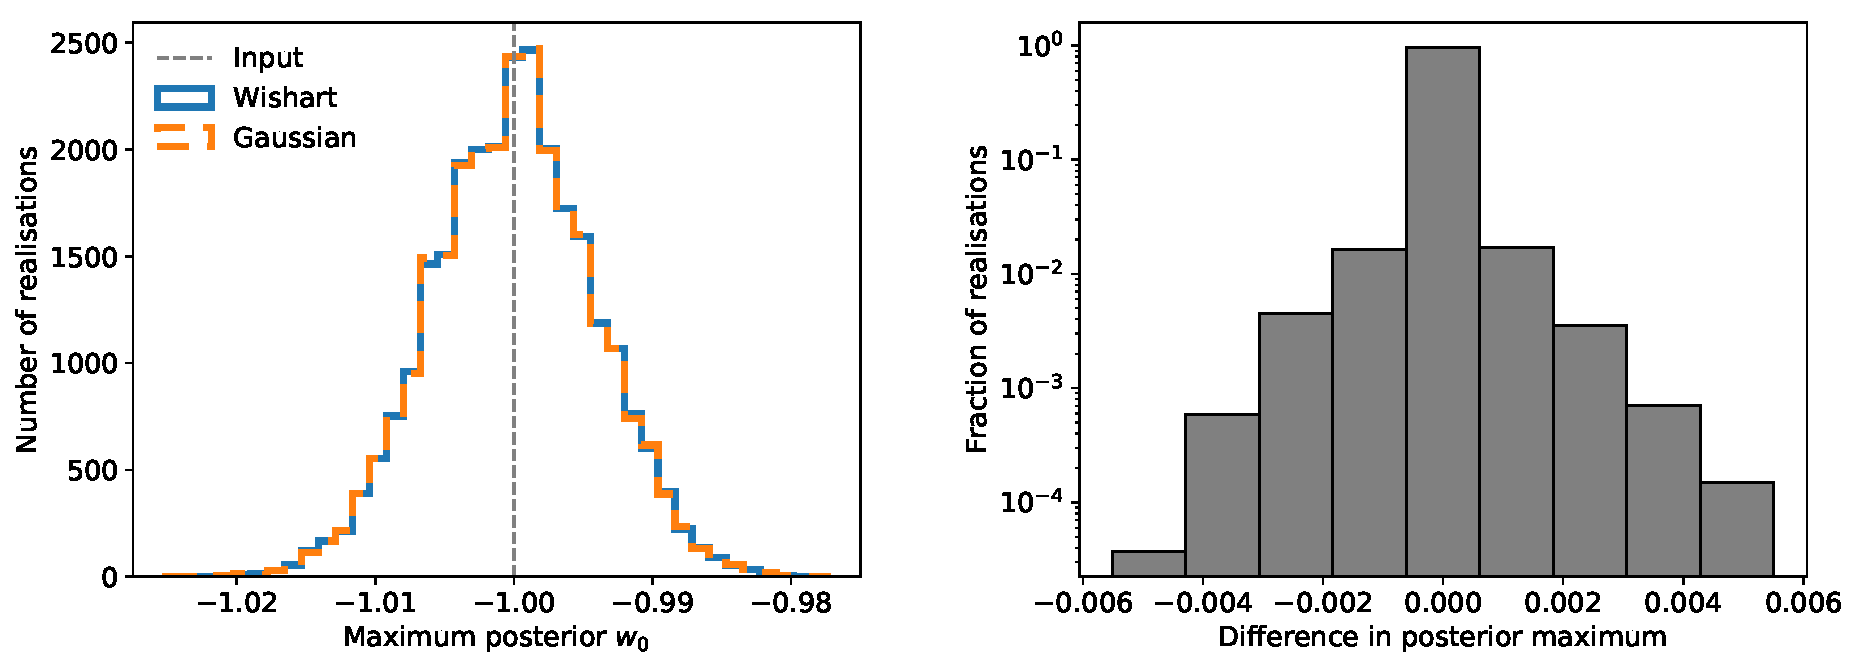
\includegraphics[width=\textwidth]{postmax}
\caption{\textit{Left:} Distribution of posterior maxima returned by the Gaussian likelihood compared to the true, Wishart likelihood. \textit{Right:} Per-realisation difference between the posterior maximum returned by the two likelihoods, with a positive difference representing a higher value of $w_0$ for the Gaussian likelihood.}
\label{gl_Fig:postmax}
\end{figure}

% For a single spin-0 field,
For a single spin-0 Gaussian field,
the Gaussian likelihood with fixed variance is guaranteed to give the same posterior maximum as the true likelihood, for a flat prior \citep{Carron2013}.
\citet{Hamimeche2008} investigated the extension to correlated fields and found that while the exactness of this relation does not hold, the Gaussian likelihood will still return the correct posterior maximum as long as the fiducial model is proportional to the model which maximises the likelihood. It is argued in that paper that for models which vary smoothly with $\ell$, this will often hold approximately even if it does not hold exactly.

The left panel of \autoref{gl_Fig:postmax} shows the distribution of posterior maxima obtained from the two likelihoods for the 27\,000 realisations. The distributions are almost indistinguishable. The right panel shows the per-realisation difference between the posterior maximum returned by the two likelihoods. The Gaussian returns the correct maximum for 95.7 per cent of the realisations, and for the remainder it is wrong by no more than four grid points, which have a size of $\Delta w_0 = 1.25 \times 10^{-3}$. This demonstrates that---as predicted in \citet{Hamimeche2008}---the maximum-posterior property of the Gaussian likelihood holds to a very good approximation in practice for correlated fields.

\subsubsection{Posterior mean and standard deviation}

\begin{figure}
\centering
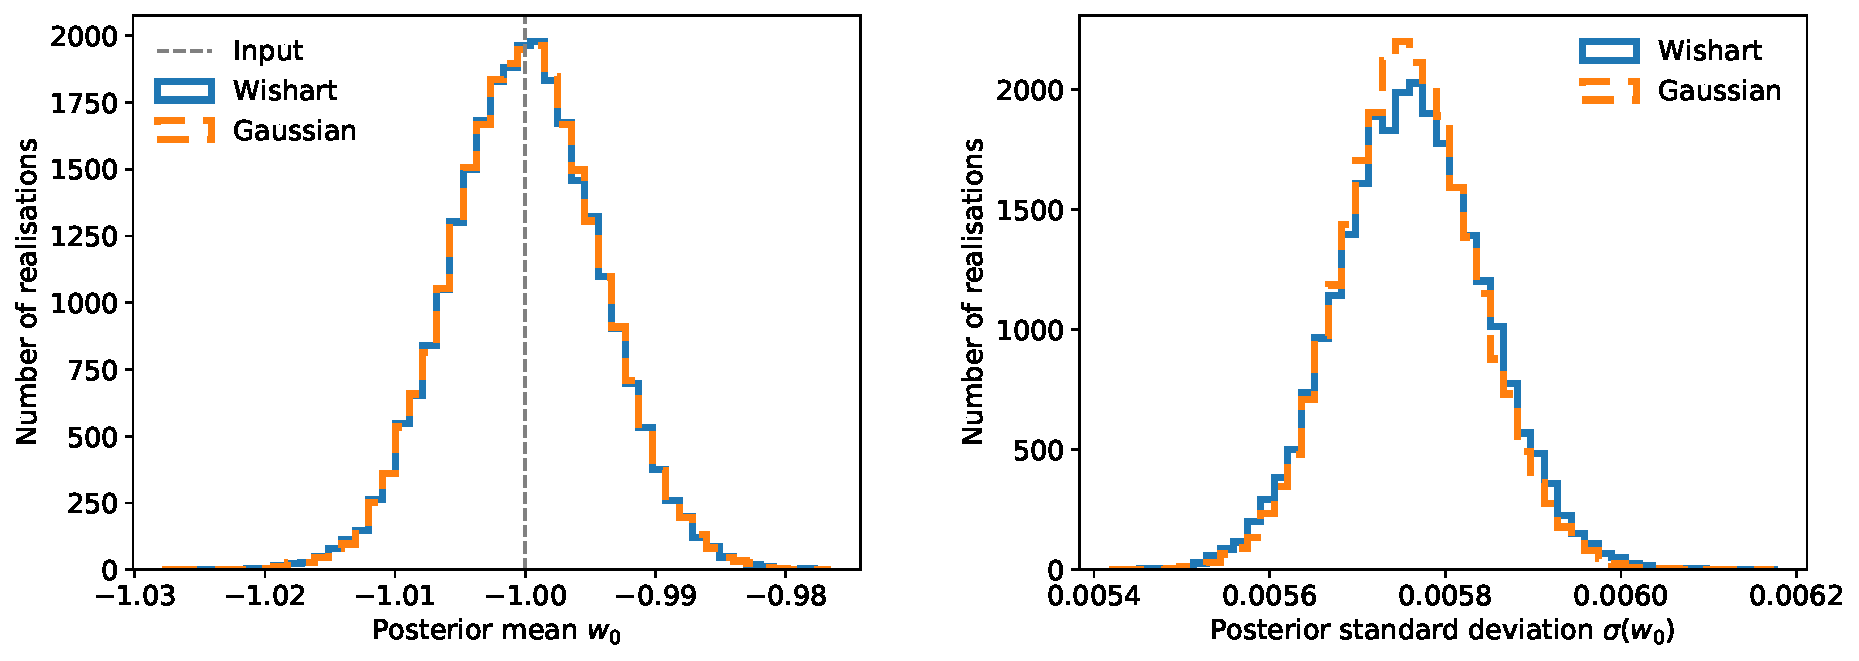
\includegraphics[width=\textwidth]{postmeanstd}
\caption{\textit{Left:} Distribution of posterior means returned by the Gaussian likelihood compared to the true, Wishart likelihood. \textit{Right:} Distribution of posterior standard deviations for the two likelihoods.}
\label{gl_Fig:postmeanstd}
\end{figure}

Along with the posterior maximum, two other summary statistics
for which it is perhaps most important for an approximate likelihood to return accurate values are the posterior mean and standard deviation. Unlike the posterior maximum, there is no general property of the Gaussian likelihood which says that it should return approximately correct values of these quantities. However, this appears to be the case on average: \autoref{gl_Fig:postmeanstd} shows the distribution of posterior means (left panel) and standard deviations (right panel) for the Gaussian likelihood compared to the true, Wishart likelihood. The distributions of means are almost indistinguishable. The distributions of standard deviations are very similar, though there is some visible discrepancy. Further investigation revealed that the Gaussian overestimates the standard deviation on realisations for which the true standard deviation is low (relative to its average over all realisations) and underestimates the standard deviation on realisations for which the true standard deviation is high. This effect has a magnitude of order 1 per cent of the true standard deviation. This is highly likely to be an acceptable level of inaccuracy, and is also expected to be smaller still when $\lmax$ is higher than the value of 100 used here.

\subsection{Full sky: Posterior contours}
\label{gl_Sec:fs_contours}

As described in \autoref{chap:est_like}, cosmological parameter constraints are often visualised using two-dimensional contour plots, with the contours representing particular credible regions. Here, the accuracy of the Gaussian likelihood is tested in this regard. A single mock observation is used, produced following the method described in \autoref{gl_Sec:fs_method_obs} with $\lmax = 2000$. This realisation was produced at random, but the results presented here have been checked with different realisations, and all give identical results in terms of level of agreement between the two likelihoods. As is the case in a real experiment, the posterior constraints are not centred on the input cosmology, due to the sizeable contribution from cosmic variance inherent in a single realisation.

In most cases, a two-parameter likelihood analysis in ($w_0$, $w_a$) is performed to keep computational costs down, but a three-parameter example is also provided to demonstrate that marginalisation over a third parameter does not affect the level of agreement between likelihoods. All two-dimensional posteriors are presented in terms of 1--3$\sigma$ contours, using the shorthand convention (see \autoref{chap:est_like}) that 1, 2 and 3$\sigma$ represent 68.3, 95.4 and 99.7 per cent posterior probability.

\subsubsection{Baseline setup}

The baseline full-sky test setup used here is as follows. The sensitivity of the results presented in this chapter to the details of this setup are tested in \autoref{gl_Sec:robustness}.
\begin{enumerate}
\item Five redshift bins (see \autoref{gl_Sec:fs_method_theory}), each with galaxy number overdensity and shear $E$-mode fields;
\item All 55 3$\times$2pt power spectra between these ten fields; i.e., galaxy--galaxy, shear--shear and galaxy--shear;
\item Gaussian noise assuming a \textit{Euclid}-like number density evenly split between bins (see \autoref{gl_Sec:fs_method_obs});
\item Multipole range $2 \leq \ell \leq 2000$;
\item Fiducial cosmology for Gaussian covariance equal to the true input cosmology used to generate the mock observation.
\end{enumerate}

\autoref{gl_Fig:3dpost} shows two- and one-dimensional marginalised posterior distributions obtained from a three-parameter likelihood analysis with the Wishart and Gaussian likelihoods. The results from the two likelihoods are visually indistinguishable, showing that under the baseline setup the Gaussian likelihood is sufficiently accurate.

\begin{figure}
\centering
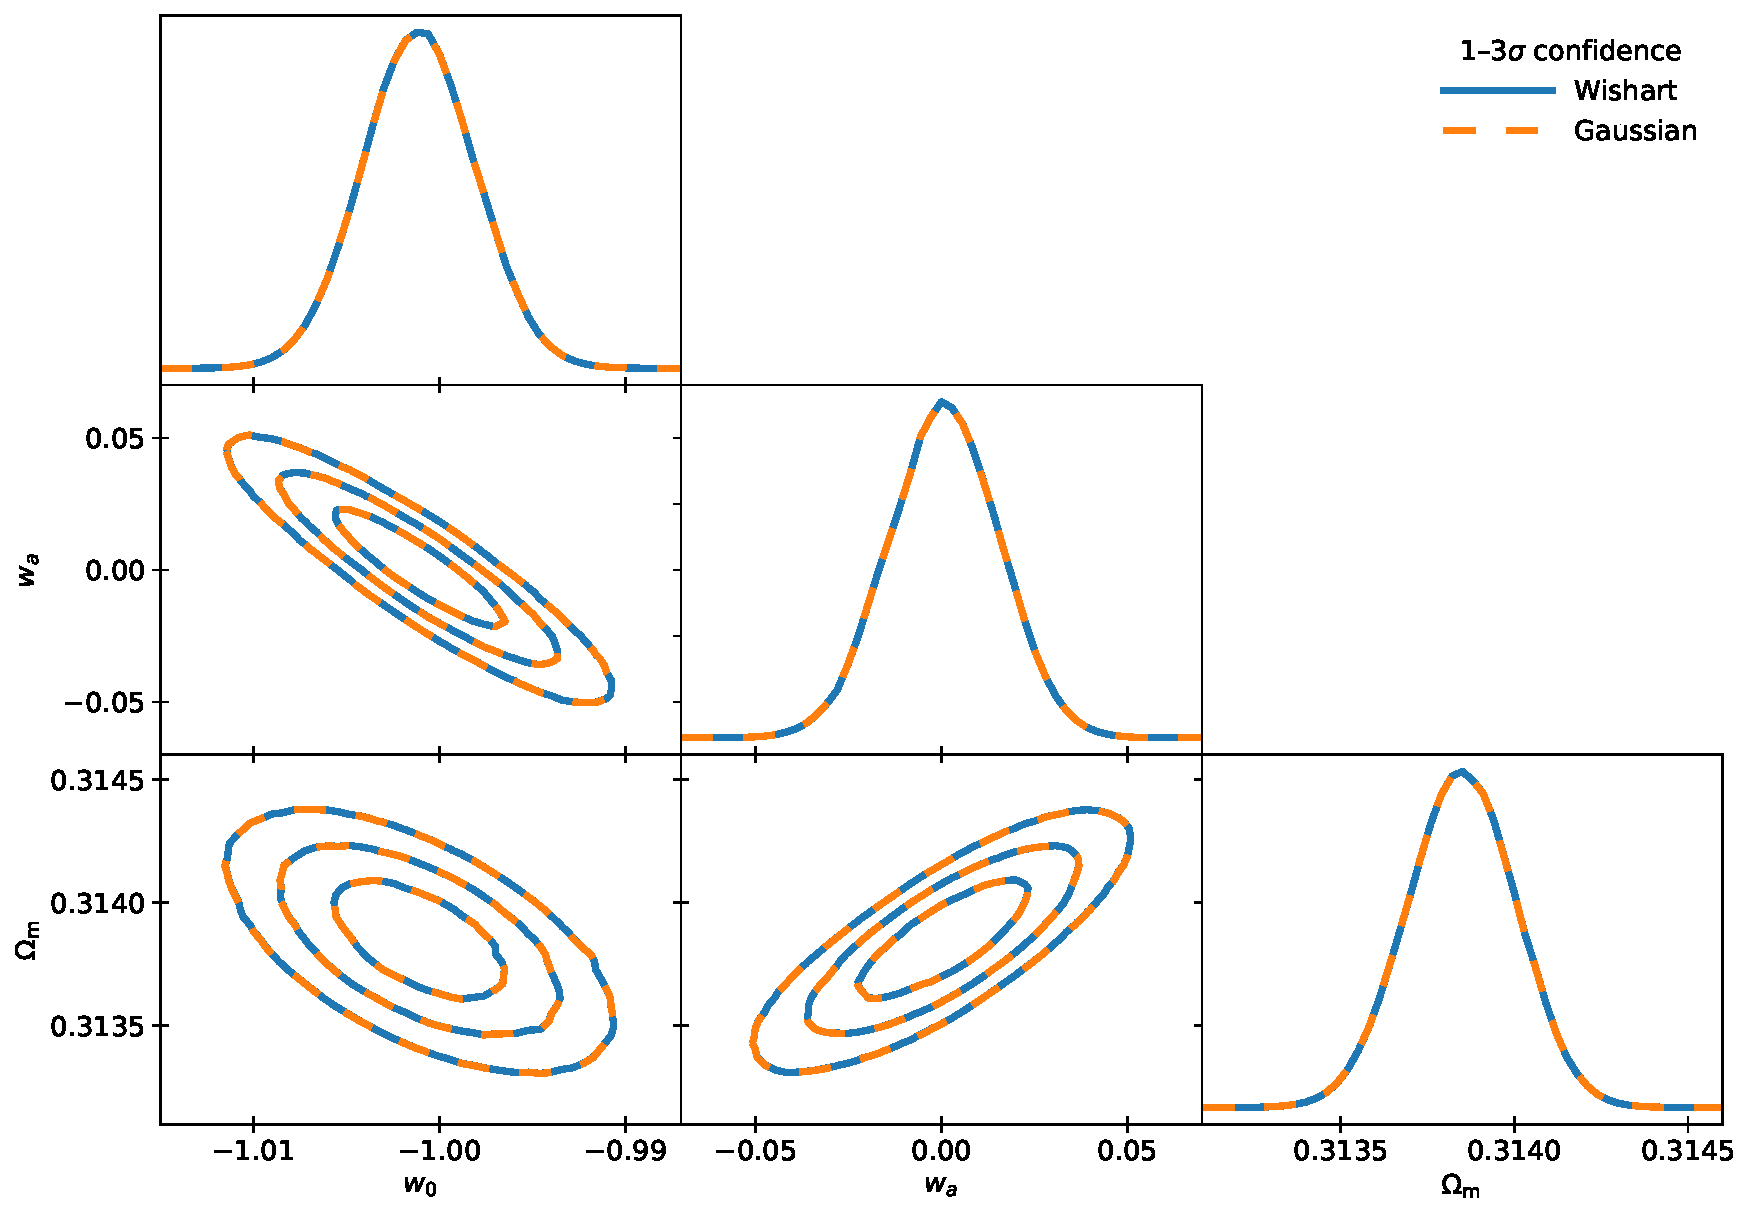
\includegraphics[width=\textwidth]{3dpost}
\caption{Two- and one-dimensional marginalised posteriors from a three-parameter likelihood analysis using the Gaussian likelihood compared to the true, Wishart likelihood.}
\label{gl_Fig:3dpost}
\end{figure}

\subsubsection{Robustness to deviation from baseline setup}
\label{gl_Sec:robustness}

It is important to check that the impressive degree of accordance between the Wishart and Gaussian likelihoods in \autoref{gl_Fig:3dpost} is not a result of any specific choices made in the baseline setup outlined above. The robustness of these results to deviations from this baseline setup is now tested. For these tests, a two-parameter likelihood analysis was performed with other parameters fixed.

\paragraph*{Fiducial cosmology}

\begin{figure}
\centering
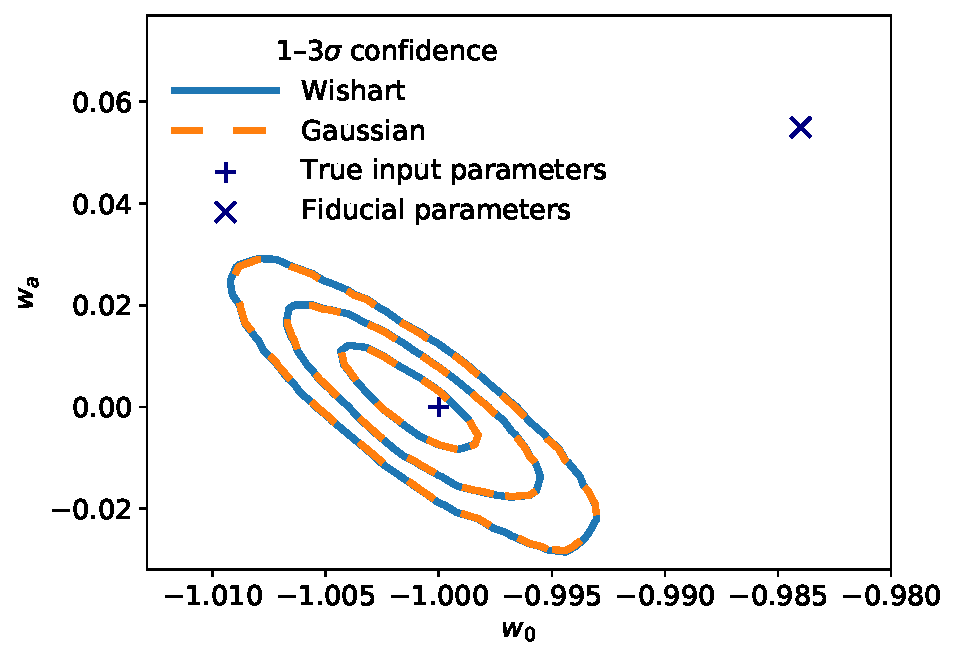
\includegraphics[width=.5\textwidth]{fid_params}
\caption{Posterior distribution of $w_0$ and $w_a$ with other parameters fixed, where the fiducial cosmology used to evaluate the Gaussian covariance is excluded at high confidence.}
\label{gl_Fig:fid_params}
\end{figure}

The Gaussian likelihood with fixed covariance requires choosing a fiducial cosmology at which to evaluate the covariance. In the baseline setup, the fiducial cosmology was chosen to be equal to the true input cosmology that was used to generate the mock observation. In a real analysis this would not be possible, since the true cosmology is unknown. To model this effect, the analysis was repeated with the fiducial cosmology chosen to be distant from the true cosmology. \autoref{gl_Fig:fid_params} shows one example, for which the fiducial cosmology is excluded at more than $10 \sigma$ and yet this does not appear to affect the accuracy of the Gaussian likelihood. Further tests showed that the accuracy does eventually diminish, but only when the fiducial cosmology and the true cosmology are unrealistically far apart (e.g. using a fiducial $w_0 = -0.2$ and a true $w_0 = -1.0$). Even in this case, it is the size and shape of the posterior distribution that is affected, much more than its location. In any real analysis, if the fiducial cosmology were excluded at high confidence then the analysis should be repeated with a fiducial cosmology consistent with the data. Therefore, even if posterior parameter constraints in the initial case were inaccurate due to the choice of fiducial cosmology, they would converge onto the correct constraints through this process.

\paragraph*{$\bm{\ell}$ range}

\begin{figure}
\centering
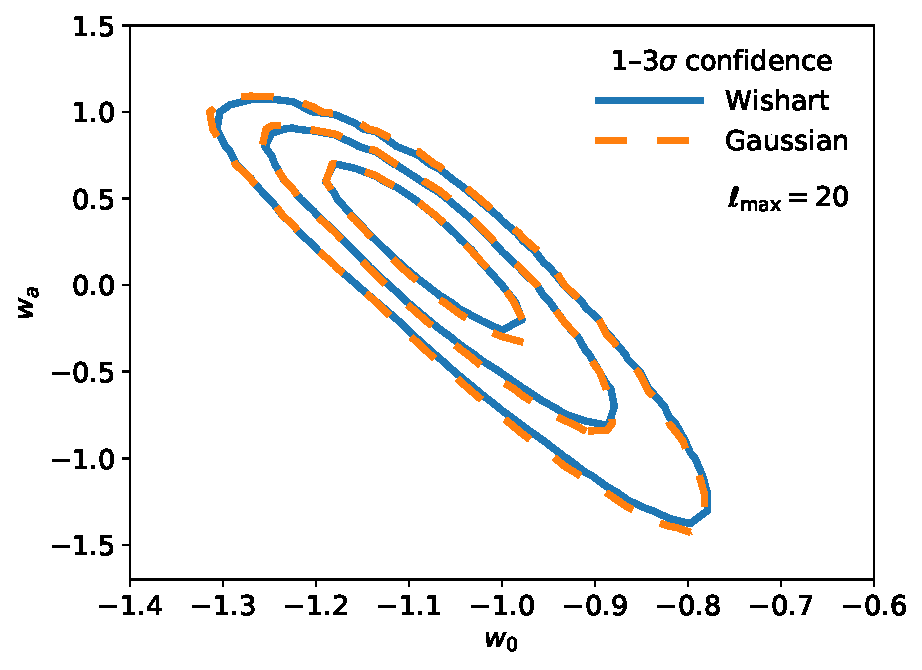
\includegraphics[width=.5\textwidth]{lmax20}
\caption{Posterior distribution of $w_0$ and $w_a$ with other parameters fixed, with only $\ell = $ 2--20 included in the likelihood.}
\label{gl_Fig:lmax20}
\end{figure}

The Gaussian likelihood should be expected to perform best at high $\ell$, as the true likelihood gradually tends to Gaussian by the central limit theorem as more $\alm$s contribute to each $\Cl$ estimate (see \autoref{gl_Sec:cut_sky}). Therefore, as $\lmax$ is reduced for a constant $\lmin$, the accuracy of the Gaussian likelihood should decrease. This expected behaviour is observed, but it is surprisingly weak. \autoref{gl_Fig:lmax20} shows the posterior distribution obtained with $\lmax = 20$. While there is some disagreement between the two sets of contours, the Gaussian likelihood is still very clearly able to recover the non-Gaussian shape of the true posterior.

\paragraph*{Noise}

\begin{figure}
\centering
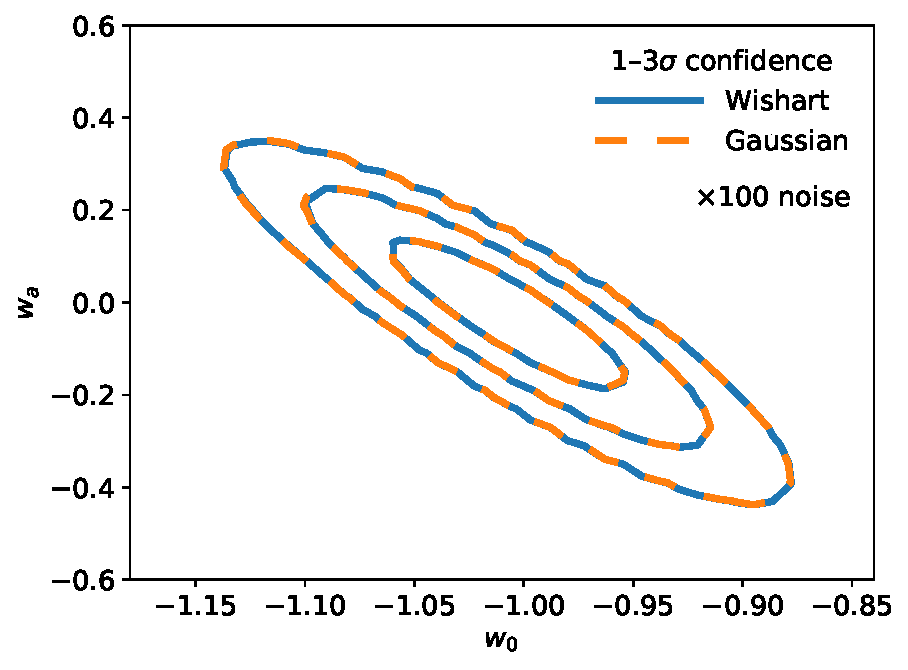
\includegraphics[width=.5\textwidth]{x100noise}
\caption{Posterior distribution of $w_0$ and $w_a$ with other parameters fixed, with noise at $100 \times$ \textit{Euclid}-like levels.}
\label{gl_Fig:x100noise}
\end{figure}

Even under the assumption of Gaussian fields and Gaussian noise, the level of noise has a theoretical impact on the accuracy of the Gaussian likelihood. This is because the noise power spectrum is flat, while the signal power spectra all decrease with $\ell$. For any noise level, there is a threshold $\ell$ above which the noise dominates the signal. Increasing the noise level decreases this threshold, meaning that a greater fraction of the overall constraining power of the data comes from lower $\ell$. Therefore, increasing the noise level relatively upweights the contribution of lower $\ell$, which---as discussed above---is the subset of the data for which the Gaussian likelihood should perform worst. However, this does not appear to have a noticeable effect for realistic noise levels. \autoref{gl_Fig:x100noise} shows the posterior distributions obtained with $100 \times$ \textit{Euclid}-like noise, achieved by assuming a total galaxy number density of $0.3 / \text{arcmin}^2$.
The effect of decreasing noise was also tested (and even switching it off entirely for a reduced two-redshift-bin setup), though for Gaussian fields and Gaussian noise this should not decrease the accuracy of the Gaussian likelihood; rather, it should increase following the inverse of the above argument. In both cases this did not lead to any visible discrepancy between the two posteriors.

Other aspects of the baseline setup were also varied, including testing with a single power spectrum and testing other parameter combinations ($\Omega_\text{m}$--$\sigma_8$, $w_0$--$n_\text{s}$, $\Omega_\text{m}$--$\sigma_8$--$w_0$) but none of these made any visible difference to the level of accordance between the two likelihoods. One change that did make a significant difference was allowing the covariance matrix in the Gaussian likelihood to vary across parameter space rather than being fixed, confirming that this aspect is crucial to the accuracy of the Gaussian likelihood. With the covariance fixed, we can conclude that the Gaussian likelihood is sufficiently accurate for full-sky power spectra from Gaussian fields.

\section{Cut-sky likelihood}
\label{gl_Sec:cut_sky}

It cannot be necessarily assumed that the accuracy of the Gaussian likelihood on the full sky will extend to the cut sky, where the situation is more complicated. Although the exact cut-sky likelihood under the assumption of Gaussian fields is known (\autoref{chap:exact_like}), it is only feasible to use in its exact form in specific low-dimensional cases.
On the full sky, all $\alm$s are independent, and are identically distributed for a given $\ell$. The introduction of a mask mixes the $\alm$s \citep{Lewis2001, Brown2005}, breaking these two properties. For an exact treatment, it becomes necessary to keep track of the relationship between all $\alm$s, which quickly becomes impossible for a high-dimensional analysis such as this one.

This motivates an alternative approach, which is taken here: after having tested the accuracy of the Gaussian likelihood on the full sky--where the exact likelihood is both known and tractable---the ways in which a sky cut might decrease this accuracy are now carefully considered.
To do this, the non-Gaussianity of the cut-sky likelihood is compared to the non-Gaussianity of the full-sky likelihood.
We can utilise Sklar's theorem, which states that any multivariate probability distribution may be separated into its marginal distributions and its dependence structure \citep{Sklar1959}.
The dependence structure is called the copula, though for clarity this term is not used here to avoid confusion with the method of forming an approximate joint distribution by combining separate approximations for marginals and the copula, commonly using a Gaussian copula, which was mentioned in \autoref{chap:exact_like} \citep[see][for more discussion of this method in a cosmological context]{Benabed2009, Sato2010, Sato2011}. The non-Gaussianity of the marginal distributions is therefore considered in \autoref{gl_Sec:ma_marginals}, and the non-Gaussianity of the dependence structure in \autoref{gl_Sec:ma_dependence}, in each case comparing between the full-sky and cut-sky likelihoods.

\subsection{Cut sky: Effect on marginal distributions}
\label{gl_Sec:ma_marginals}

The investigation into the non-Gaussianity of marginal distributions focuses on auto- \linebreak spectra, which by their positive-definite nature are much more non-Gaussian than cross-spectra on both the full and cut sky (\cite{Percival2006}; \autoref{chap:exact_like}).
Non-Gaussianity is here quantified using the skewness and excess kurtosis, following \citet{Lin2020} and \citet{DiazRivero2020}, since both vanish for a Gaussian distribution. These can be written in terms of the mean $E \left[ X \right]$ and standard deviation $\text{Std} \left( X \right)$ of a random variable $X$ as
\begin{align}
&\text{Skew} \left( X \right) =
E \left[ \left( \frac{X - E \left[ X \right]}
{ \text{Std} \left( X \right) } \right)^3 \right]; \\
&\text{Ex kurt} \left( X \right) =
E \left[ \left( \frac{X - E \left[ X \right]}
{ \text{Std} \left( X \right) } \right)^4 \right] - 3.
\end{align}

The marginal distribution of a full-sky auto-$C_\ell$ (the diagonal elements of Equation \ref{gl_Eqn:obs_cl_matrix}) is a gamma distribution, which under the ($k$, $\theta$) parametrisation has PDF
\begin{equation}
f_\Gamma \left( x | k, \theta \right) =
\frac{x^{k - 1} \exp \left[ - x / \theta \right]}
{\Gamma (k) \theta^k},
\end{equation}
where $\Gamma$ is the gamma function. This distribution has skewness and excess kurtosis
\begin{align}
\text{Skew} \left( X \right) &= \frac{2}{\sqrt{k}}; \\
\text{Ex kurt} \left( X \right) &= \frac{6}{k}.
\end{align}

The full-sky likelihood corresponds to parameter values
(\cite{Percival2006}; Hami-meche \& Lewis \citeyear{Hamimeche2008}; \cite{Sellentin2018a})
\begin{equation}
\widehat{C}_\ell \sim \Gamma \left(
k = \frac{2 \ell + 1}{2},~
\theta = \frac{2 C_\ell}{2 \ell + 1} \right).
\end{equation}

Both the skewness and kurtosis therefore depend only on $\ell$, and are both power laws in $2 \ell + 1$:
\begin{align}
&\text{Skew} \left( \widehat{C}_\ell \right)
= \sqrt{8} \left[ 2 \ell + 1 \right]^{- 1/2};
\label{gl_Eqn:skew_fs} \\
&\text{Ex kurt} \left( \widehat{C}_\ell \right)
= 12 \left[ 2 \ell + 1 \right]^{-1}.
\label{gl_Eqn:kurt_fs}
\end{align}
The skewness and excess kurtosis of the cut-sky likelihood may be derived from the pseudo-$C_\ell$ marginal characteristic function (CF),
\begin{equation}
\varphi_{\widetilde{C}_\ell} \left( t \right) = \prod_j
\left( 1 - 2i \lambda_j t \right)^{-1/2},
\label{gl_Eqn:marg_cf}
\end{equation}
where $\{ \lambda_j \}$ are the eigenvalues of
$\mathbfss{M} \bm{\Sigma}$, the product of the pseudo-$a_{\ell m}$ covariance matrix $\bm{\Sigma}$ with $\mathbfss{M}$, the selection matrix picking out the relevant elements of $\bm{\Sigma}$ for the $C_\ell$ in question (see \autoref{chap:exact_like}). Equation \eqref{gl_Eqn:marg_cf} may be identified as a product of gamma distribution CFs:
\begin{equation}
\varphi_\Gamma \left( t \right) =
\left( 1 - \theta i t \right)^{-k},
\end{equation}
each with parameters $k = 1/2$, $\theta = 2 \lambda_j$. Since the CF of a sum of independent random variables is equal to the product of the individual CFs, it follows that the marginal distribution of a pseudo-$C_\ell$ estimate is identical to that of a sum of independent gamma-distributed variables. This allows the calculation of the cut-sky skewness and excess kurtosis in terms of the eigenvalues $\lambda_j$ of $\mathbfss{M} \bm{\Sigma}$:
\begin{align}
\text{Skew} \left( \widetilde{C}_\ell \right)
&= \frac{ 2^{3/2} \sum_j \lambda_j ^3 }
{ \left[ \sum_j \lambda_j^2 \right]^{3 / 2}};
\label{gl_Eqn:skew_ma} \\[1em]
\text{Ex kurt} \left( \widetilde{C}_\ell \right)
&= \frac{12 \sum_j \lambda_j^4}
{\left[ \sum_j \lambda_j^2 \right]^2}.
\label{gl_Eqn:kurt_ma}
\end{align}

\begin{figure}
\centering
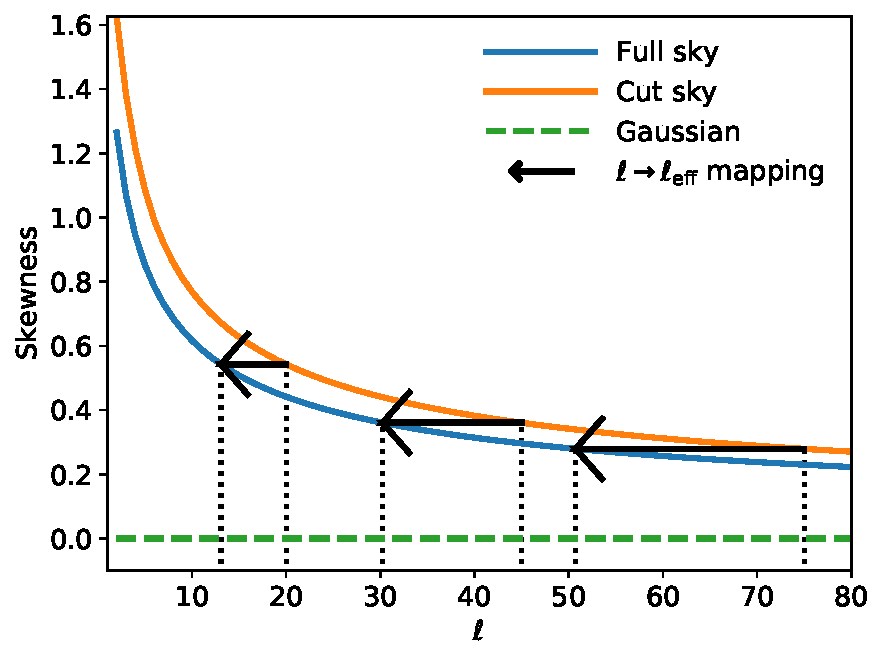
\includegraphics[width=.5\textwidth]{skewness}
\caption{Skewness of the full-sky and cut-sky marginal auto-$C_\ell$ distribution as a function of $\ell$, where the cut-sky result is for a \textit{Euclid}-like mask. The arrows demonstrate the $\ell \rightarrow \leff$ mapping described in \autoref{gl_Sec:ma_marginals_impact}.}
\label{gl_Fig:skewness}
\end{figure}

\autoref{gl_Fig:skewness} shows the full- and cut-sky skewness as a function of $\ell$, up to $\ell = 80$, for a \textit{Euclid}-like mask incorporating the survey footprint and a bright star mask ($f_\text{sky} = 30.7$ per cent). Both curves are smoothly decreasing, with the cut-sky skewness systematically higher. The kurtosis exhibits a similar behaviour. The marginal distributions of the likelihood, therefore, are more non-Gaussian on the cut sky than on the full sky. The impact of this additional non-Gaussianity is now investigated.

\subsubsection{Impact of additional non-Gaussianity}
\label{gl_Sec:ma_marginals_impact}

\begin{figure}
\centering
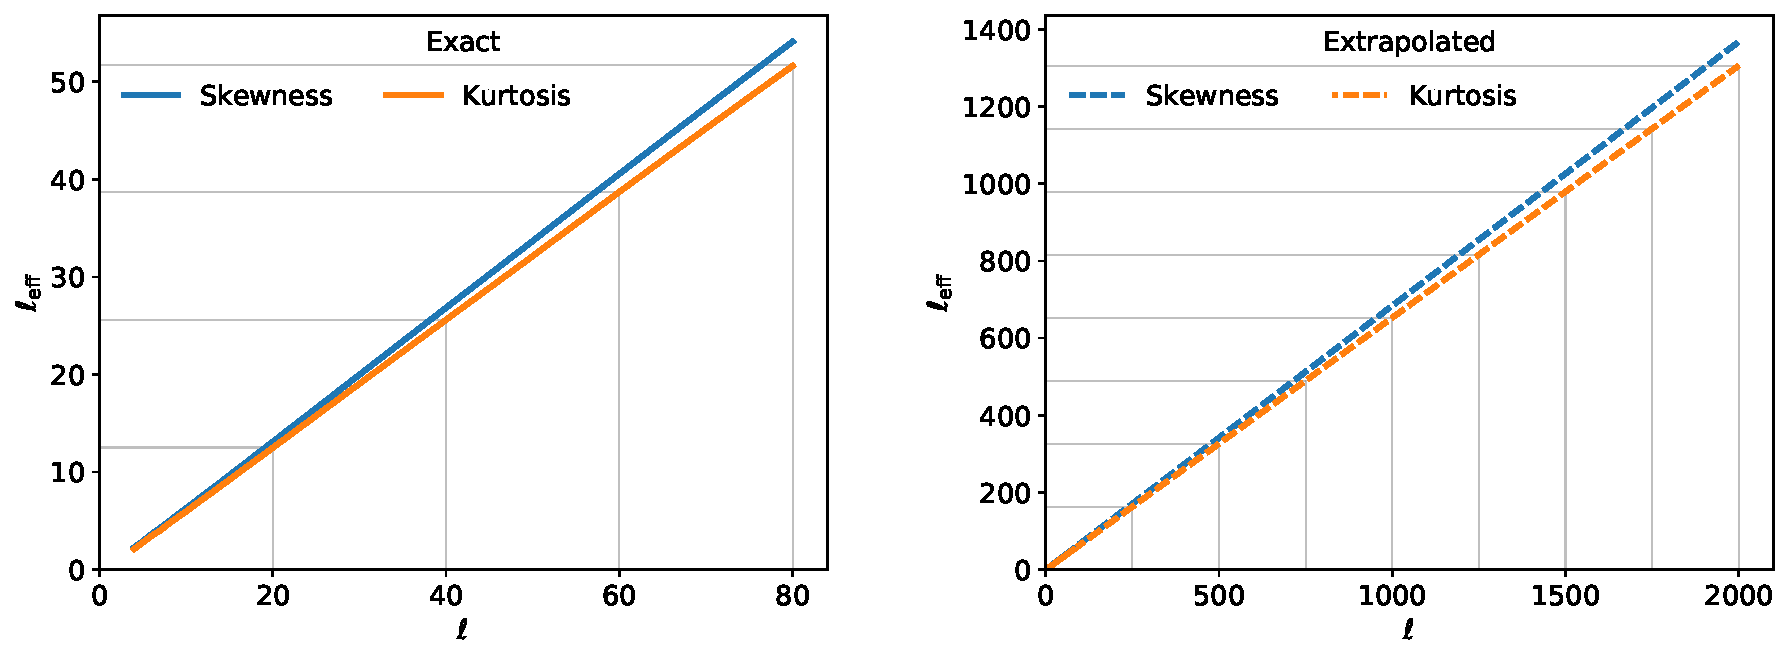
\includegraphics[width=\textwidth]{leff_map}
\caption{\textit{Left:} $\ell \rightarrow \leff$ mapping derived from equating the skewness (blue) and excess kurtosis (orange) of the full-sky and cut-sky likelihoods. \textit{Right:}~Extrapolated to $\ell = 2000$.}
\label{gl_Fig:leff_map}
\end{figure}

\begin{figure}
\centering
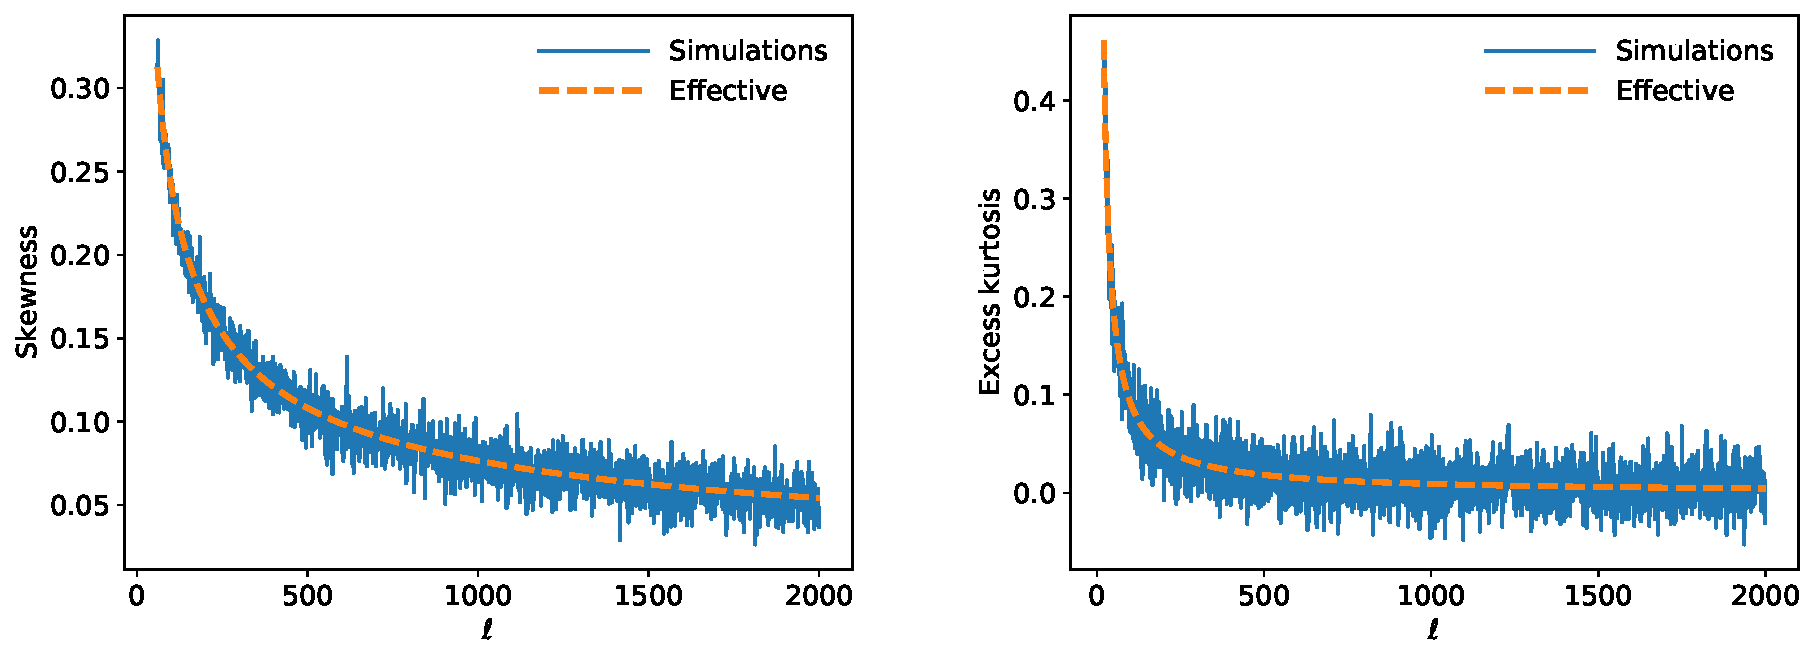
\includegraphics[width=\textwidth]{leff_validation}
\caption{Validation of the extrapolation in \autoref{gl_Fig:leff_map} against 63\,100 simulated cut-sky realisations.}
\label{gl_Fig:leff_validation}
\end{figure}

We can take advantage of the fact that both skewness and kurtosis are higher on the cut sky and that both decrease smoothly with $\ell$ to define an `effective $\ell$', $\leff$, for each $\ell$ by equating the full- and cut-sky skewness, and the same for kurtosis. This process is demonstrated by the arrows in \autoref{gl_Fig:skewness}. This $\ell \rightarrow \leff$ mapping is shown in the left panel of \autoref{gl_Fig:leff_map}, and turns out to be perfectly linear for both skewness and kurtosis. This is unexpected, since it is not apparent from the expressions for the full- and cut-sky skewness and excess kurtosis in Equations \eqref{gl_Eqn:skew_fs}--\eqref{gl_Eqn:kurt_fs} and \eqref{gl_Eqn:skew_ma}--\eqref{gl_Eqn:kurt_ma}. However, additional tests have confirmed that it holds for all ten auto-spectra in this setup. It appears that the cut-sky skewness and excess kurtosis as a function of $\ell$ are simply linear transformations of their full-sky counterparts, with the slope of the transformation depending on the details of the mask.

In the right panel of \autoref{gl_Fig:leff_map}, this linear mapping is extrapolated to $\ell = 2000$. Since this is a large extrapolation, it is verified in \autoref{gl_Fig:leff_validation} by comparing to the sample skewness and kurtosis from 63\,100 simulated cut-sky realisations of a single field. It is clearly an excellent fit.

Finally, the impact of this additional non-Gaussianity of the marginal distributions on the cut sky is tested by applying an adjusted Wishart likelihood having the correct amount of cut-sky non-Gaussianity in its marginal distributions, which is obtained by replacing $\ell$ in the likelihood with $\leff$. The kurtosis mapping is used here, since it gives a lower $\leff$ for a given $\ell$ (\autoref{gl_Fig:leff_map}) and is therefore a more pessimistic choice. The adjusted likelihood replaces Equation \eqref{gl_Eqn:wishart} with
\begin{equation}
\widehat{\mathbfss{C}}'_\ell \sim
\mathcal{W} \left( \nu = 2 \leff + 1,
\mathbfss{V} = \frac{\mathbfss{C}_\ell}{2 \leff + 1} \right).
\label{gl_Eqn:adj_wishart}
\end{equation}

Note that each observed $\ell$ still depends on the same $\ell$ in the theory power spectra. This means that each $\Cl$ will retain the correct sensitivity to cosmological parameters, enabling a test of the impact of an increased amount of non-Gaussianity for the same cosmological constraining power. The marginal distributions of the auto-$\Cl$s in $\widehat{\mathbfss{C}}'_\ell$ are gamma distributions, with parameters
\begin{equation}
\widehat{C}'_\ell \sim \Gamma \left(
k = \frac{2 \leff + 1}{2},~
\theta = \frac{2 C_\ell}{2 \leff + 1} \right),
\end{equation}
and therefore---from Equations \eqref{gl_Eqn:skew_fs}--\eqref{gl_Eqn:kurt_fs}---will have the same amount of skewness and excess kurtosis as the cut-sky likelihood (in fact a slightly higher amount of skewness, since the kurtosis $\ell \rightarrow \leff$ mapping is used).

The corresponding Gaussian likelihood has the same mean and covariance as the adjusted Wishart likelihood. Its mean, therefore, is unchanged from the full-sky case, while the covariance is
\begin{equation}
\text{Cov} \left(
\widehat{C}_\ell^{\alpha \beta},
\widehat{C}_{\ell'}^{\gamma \varepsilon}
\right)
= \frac{\delta_{\ell \ell'}}{2 \leff + 1} \left(
C_\ell^{\alpha \gamma} C_\ell^{\beta \varepsilon}
+ C_\ell^{\alpha \varepsilon} C_\ell^{\beta \gamma} \right).
\end{equation}

\begin{figure}
\centering
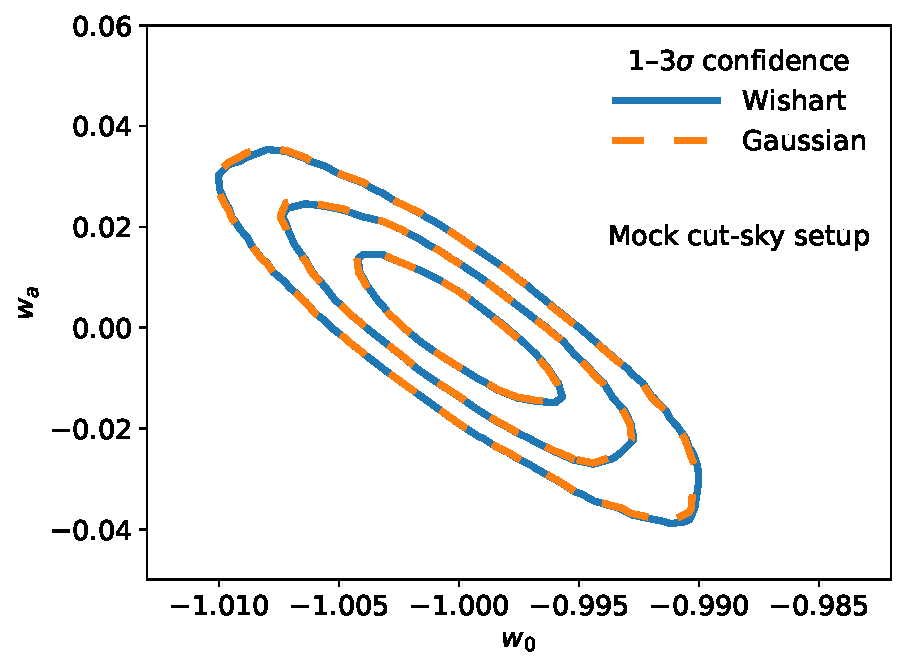
\includegraphics[width=.5\textwidth]{leff_post}
\caption{Posterior distributions obtained from a mock observation designed to have the same amount of non-Gaussianity in its marginal distributions as the cut-sky likelihood.}
\label{gl_Fig:leff_post}
\end{figure}

A mock observation following Equation \eqref{gl_Eqn:adj_wishart} was generated by sampling directly from the Wishart distribution using the \texttt{SciPy} implementation of the Wishart variate generating algorithm from \citet{Smith1972}. Using this observation, a two-parameter likelihood analysis was conducted with the adjusted Wishart and Gaussian likelihoods. The resulting posterior distribution is shown in \autoref{gl_Fig:leff_post}. There is very good agreement between the two likelihoods. Although small deviations are visible, this is highly likely to be an acceptable level of inaccuracy.

We can therefore conclude that the additional non-Gaussianity in the marginal distributions of the cut-sky likelihood compared to the full-sky likelihood is insufficient to introduce significant inaccuracy into the results obtained using a Gaussian likelihood.

\subsection{Cut sky: Effect on dependence structure}
\label{gl_Sec:ma_dependence}

To study the cut-sky dependence structure it is necessary to rely on simulations. 50\,000 simulated observations were generated, following the method described in \autoref{gl_Sec:fs_method_obs} with two differences: first, the observed power spectra were measured for each realisation both before and after multiplication at the map level by the \textit{Euclid}-like mask; 10 logarithmically spaced bandpowers from $\ell =$ 2 to 2000 were then formed, weighted following Equation 20 of \citet{Hivon2002}.

\subsubsection{Mutual information}

Dependence between two data elements can be quantified using mutual information (MI). MI is defined as the Kullback--Leibler (KL) divergence $D_\text{KL}$ of the joint distribution of two variables from the product of their marginal distributions,
\begin{equation}
I \left( X, Y \right)
= D_\text{KL} \left( P_{\left( X, Y \right)} ~\middle| \middle|~
P_X \otimes P_Y \right),
\end{equation}
where the KL divergence for continuous distributions is
\begin{equation}
D_\text{KL} \left( P_{\left( X, Y \right)} ~\middle| \middle|~
P_X \otimes P_Y \right)
= \iint dx\,dy ~ p \left( x, y \right)
\log \left( \frac{ p \left(x, y \right) }
{p \left(x \right) p \left( y \right)} \right).
\label{gl_Eqn:kl_div}
\end{equation}

If $X$ and $Y$ are independent, their joint distribution factorises and the MI vanishes. If they are not independent, they will have a positive MI. In practice, however, MI estimation from a finite number of samples may return a negative value.

To isolate non-Gaussian dependence, a whitening procedure is first applied to remove linear correlations. Linear correlations are those which are fully described by a covariance (or equivalently, correlation) matrix. Since the dependence structure in a multivariate Gaussian distribution is also fully described by its covariance matrix---such that the components of a multivariate Gaussian with diagonal covariance are independent---removing linear correlations removes all Gaussian dependence.
This whitening follows the same process as \citet{Sellentin2018}, \citet{Sellentin2018a}, \citet{DiazRivero2020} and \citet{Louca2020}: each pair of data elements is whitened separately using a Cholesky whitening procedure followed by a mean subtraction. The result is a whitened pair having a mean of zero and a covariance matrix of the identity matrix. Each pair is whitened separately so that pairs are still identifiable, allowing the study of the behaviour of pairs with specific relationships.

For each whitened pair, MI is estimated using the Non-parametric Entropy Estimation Toolbox (\texttt{NPEET})\footnote{\url{https://github.com/gregversteeg/NPEET}} \citep{VerSteeg2014}. The \texttt{NPEET} MI estimator implements a $k$-nearest neighbours method described in \citet{Kraskov2004}. The default parameters of $k = 3$ and log base 2 are used in Equation \eqref{gl_Eqn:kl_div}.

\begin{figure}
\centering
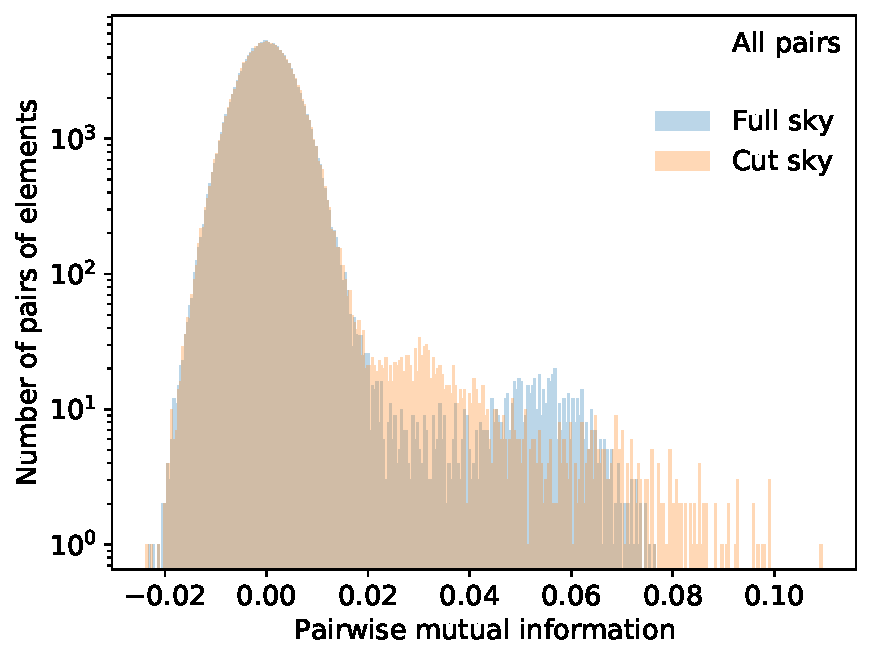
\includegraphics[width=.5\textwidth]{mi_all}
\caption{Comparison of non-Gaussian dependence between full-sky and cut-sky likelihoods. Non-Gaussian dependence is quantified by pairwise mutual information after whitening. The mass centred around zero on the $x$-axis represents Gaussian dependence, with the tail (here $\gtrsim 0.02$) representing non-Gaussian dependence.}
\label{gl_Fig:mi_all}
\end{figure}

\begin{figure}
\centering
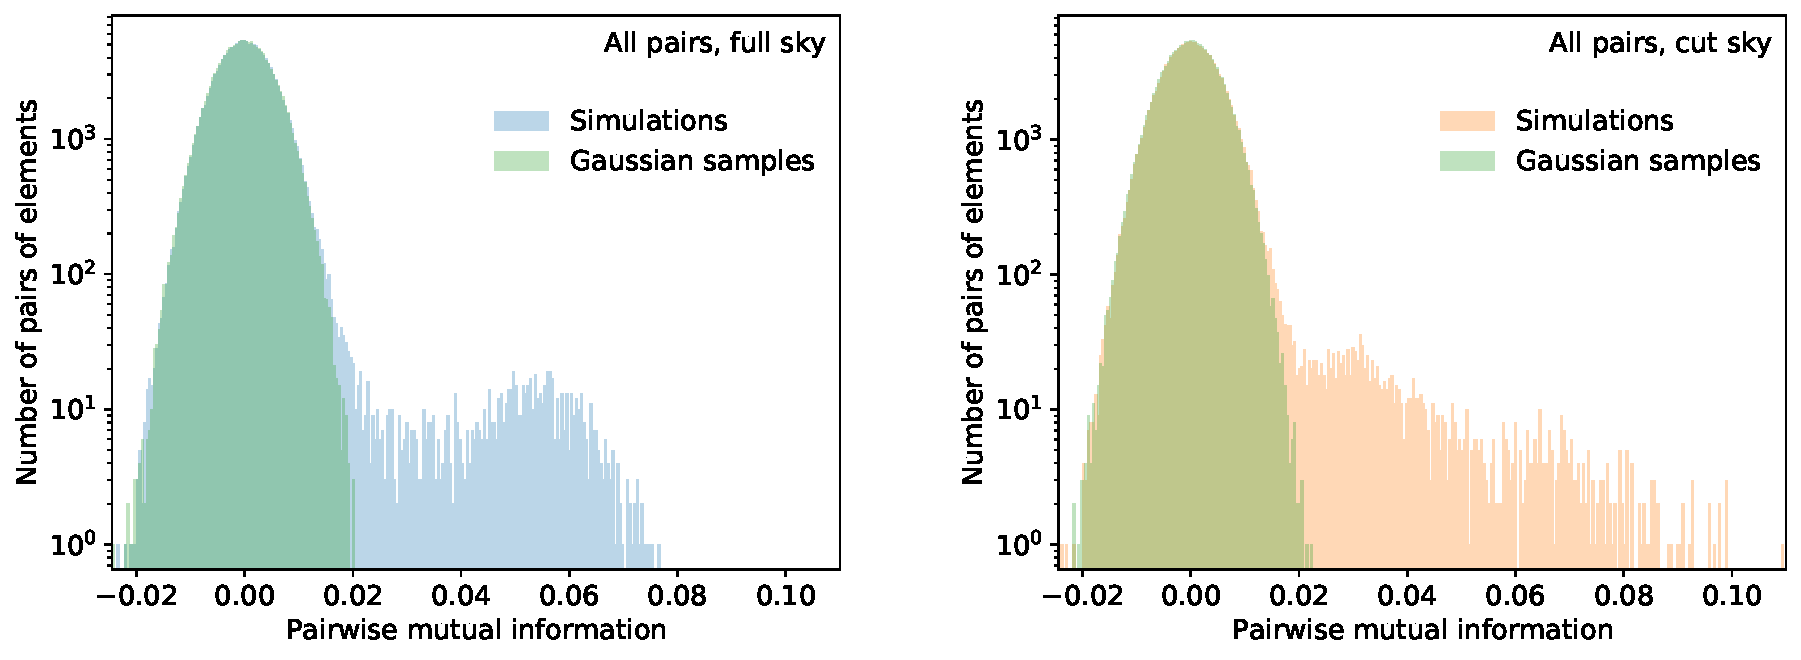
\includegraphics[width=\textwidth]{mi_vs_gauss}
\caption{Comparison of non-Gaussian dependence between full-sky (left) and cut-sky (right) likelihoods. Non-Gaussian dependence is quantified by pairwise mutual information after whitening. In both panels the corresponding distribution for pure Gaussian dependence is shown, which is centred around zero on the $x$-axis. The tail (here $\gtrsim 0.02$) represents non-Gaussian dependence.}
\label{gl_Fig:mi_vs_gauss}
\end{figure}

\autoref{gl_Fig:mi_all} shows the distribution of pairwise whitened MI compared between full-sky and cut-sky bandpowers. Most of the pairs of elements are found in the part of the distribution centred around zero, indicating no detected non-Gaussian dependence. This is more clearly seen in \autoref{gl_Fig:mi_vs_gauss}, in which each of the full-sky and cut-sky samples is compared to an equivalent sample drawn from a multivariate Gaussian distribution having the same mean and covariance. Non-Gaussian dependence is exhibited by the pairs of elements found in the tail, in this case with MI $\gtrsim 0.02$. This tail contains only a small fraction of pairs in both cases, but with a slight excess for the cut-sky sample: 0.93 per cent of cut-sky pairs have MI $> 0.02$, compared to 0.65 per cent of full-sky pairs. This is also evident in the small visible excess of cut-sky pairs in \autoref{gl_Fig:mi_all}.

To investigate the origin of this small excess in non-Gaussian dependence for the cut-sky sample relative to the full-sky sample, each sample is split into different pair populations, corresponding to particular relationships between data elements.
Non-Gaussian dependence is almost exclusively found in pairs containing the same bandpower across correlated fields.
The strongest such case is shown in the left panel of \autoref{gl_Fig:mi_parent}, which shows pairs containing one bandpower from a cross-spectrum and the same bandpower from one of its `parent' auto-spectra, i.e. the auto-spectrum of one of the two fields between which the cross-spectrum is describing the correlation. While most pairs still appear consistent with zero, there is a significant tail of non-Gaussian dependence, which is slightly larger for the cut-sky sample. This tail is not found when looking at pairs of different bandpowers between the same two spectra, shown in the right panel of \autoref{gl_Fig:mi_parent}.
A similar behaviour is found in other same-bandpower pairs, which is strongest when the two spectra in the pair relate directly to the same underlying field; for example, two `sibling' cross-spectra which share one parent auto-spectrum. In most such pair populations, there is a slight excess of non-Gaussian dependence for the cut-sky sample.

\begin{figure}
\centering
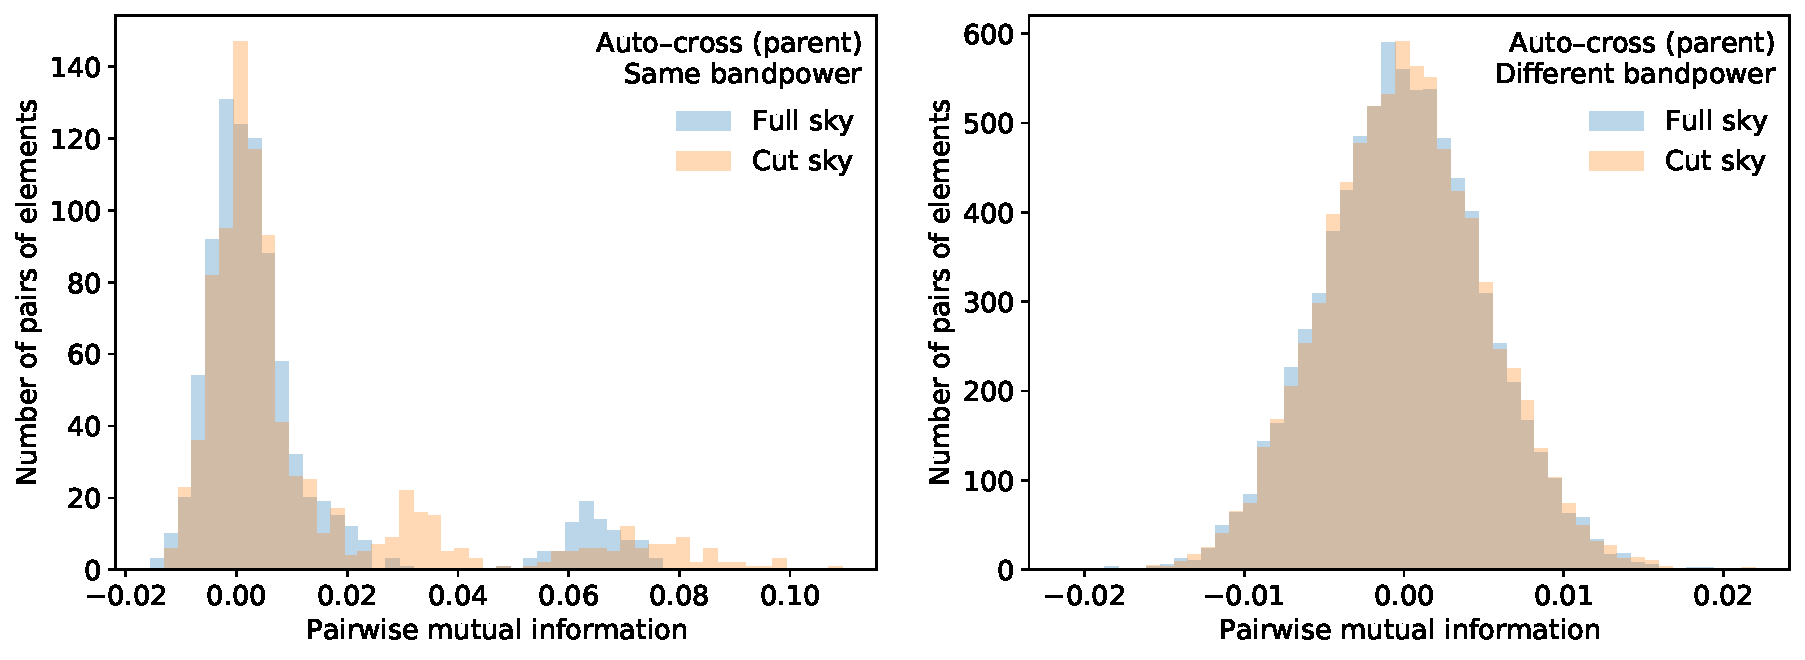
\includegraphics[width=\textwidth]{mi_parent}
\caption{Comparison of non-Gaussian dependence between full-sky and cut-sky likelihoods, for two specific populations of data element pairs. The left panel shows pairs containing the equivalent bandpower of one cross-spectrum and one of its `parent' auto-spectra (e.g. $P_b^{12}$ and $P_b^{11}$). The right panel is for different-bandpower pairs in the same combinations of spectra (e.g. $P_b^{12}$ and $P_{b'}^{11}$). Non-Gaussian dependence is quantified by pairwise mutual information after whitening. The bulk centred around zero on the $x$-axis represents Gaussian dependence, with the tail representing non-Gaussian dependence. The absence of this tail in the right panel indicates that those pairs exhibit only Gaussian dependence.}
\label{gl_Fig:mi_parent}
\end{figure}

\begin{figure}
\centering
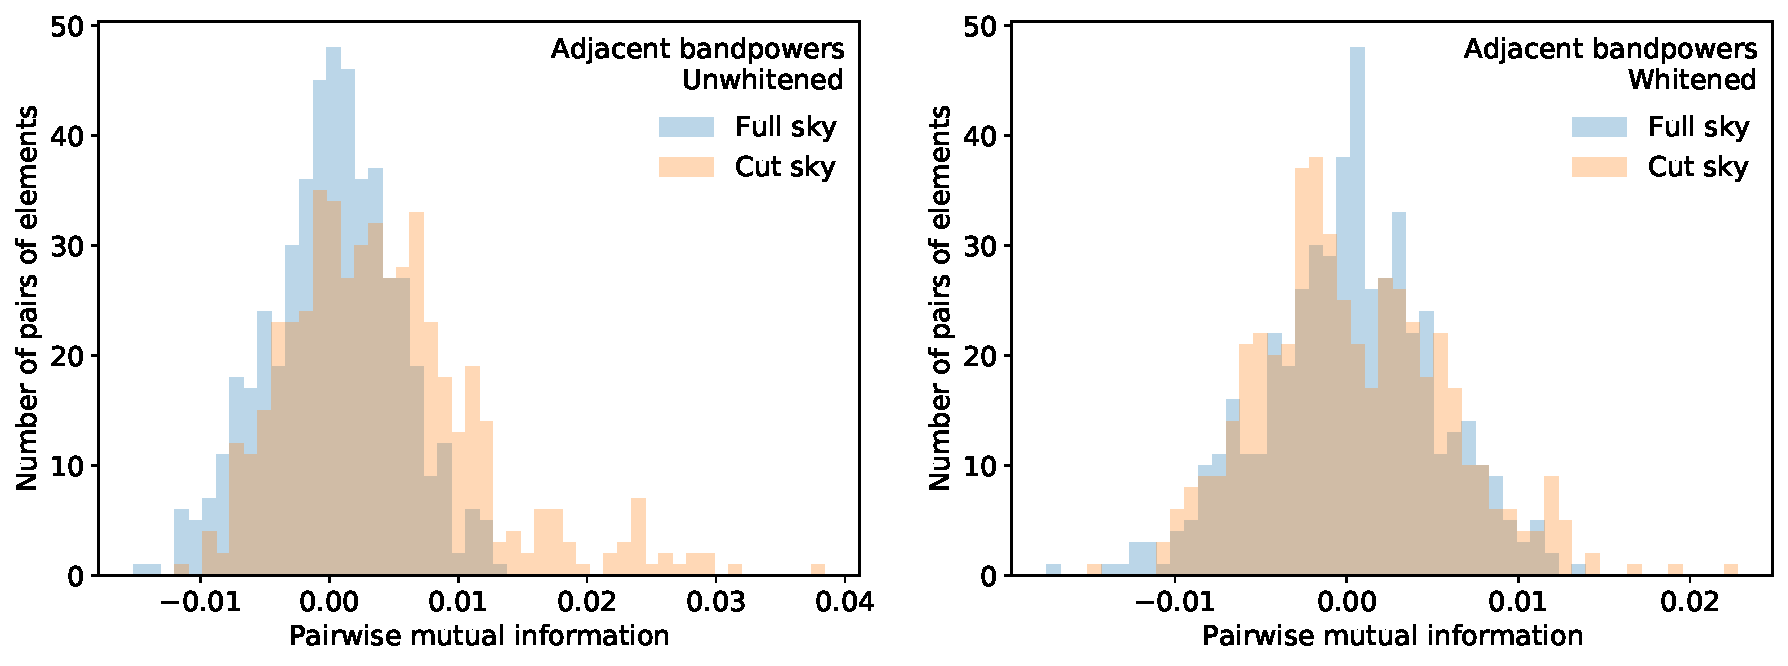
\includegraphics[width=\textwidth]{mi_adj_bp}
\caption{Full-sky and cut-sky distributions of pairwise mutual information (MI) before (left) and after (right) pairwise whitening, for pairs of adjacent bandpowers in the same spectrum (e.g. $P_b^{12}$ and $P_{b + 1}^{12}$). Prior to whitening, MI captures all dependence; in this case there is a substantial excess of dependence in the cut-sky likelihood. Whitening removes Gaussian dependence such that after whitening, MI only captures non-Gaussian dependence; in this case there is little or no excess dependence in the cut-sky likelihood.  This demonstrates that the additional dependence between adjacent bandpowers induced by a mask is mostly or wholly Gaussian.}
\label{gl_Fig:mi_adj_bp}
\end{figure}

In contrast, it turns out that the dependence between bandpowers in the same spectrum known to be induced by a cut sky in fact comprises almost purely linear correlations. This is shown in \autoref{gl_Fig:mi_adj_bp}, which compares these pairs before and after the whitening process. The left panel shows the unwhitened result, which includes linear correlations, showing an expected cut-sky excess. After whitening, shown in the right panel, this excess is almost entirely removed.

\subsubsection{Impact of additional non-Gaussian dependence}

The above section has shown that there is a small excess in non-Gaussian dependence in the cut-sky likelihood compared to the full-sky likelihood. As was done for the marginal distributions in \autoref{gl_Sec:ma_marginals_impact}, the potential impact of this additional non-Gaussianity on the accuracy of constraints obtained using the Gaussian likelihood is now investigated.

\begin{figure}
\centering
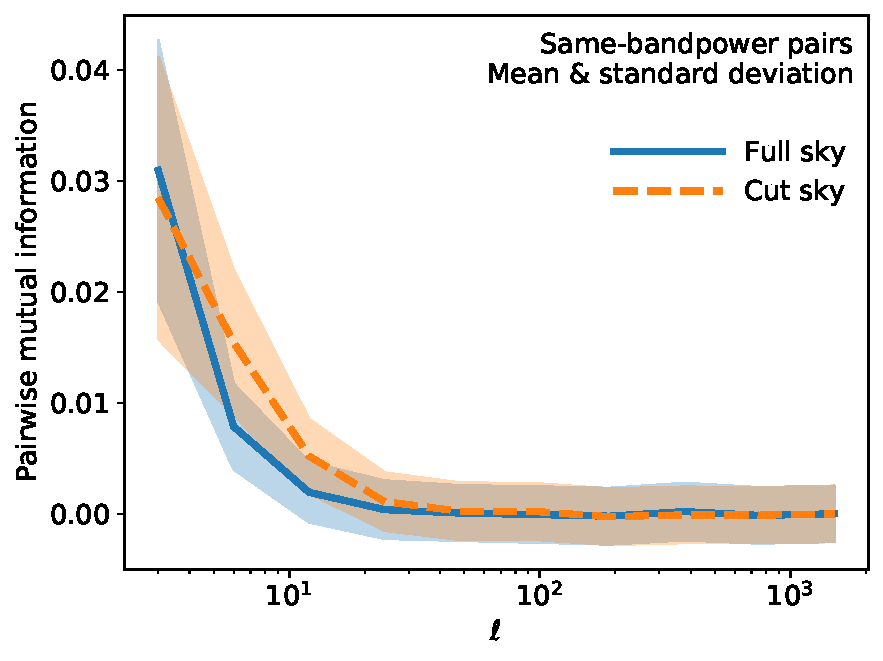
\includegraphics[width=.5\textwidth]{mi_vs_l}
\caption{Non-Gaussian dependence as a function of $\ell$, compared between full-sky and cut-sky likelihoods. Non-Gaussian dependence is quantified by pairwise mutual information after whitening, and is here averaged over all same-bandpower pairs in a given $\ell$ bin, with the shaded region containing one standard deviation.}
\label{gl_Fig:mi_vs_l}
\end{figure}

On closer inspection it turns out that the increased non-Gaussian dependence in the cut-sky likelihood is in fact an $\ell$-dependent effect. This is demonstrated in \autoref{gl_Fig:mi_vs_l}, which shows whitened MI as a function of $\ell$ for same-bandpower pairs, which as discussed above are those which exhibit non-Gaussian dependence. Non-zero MI appears to be restricted only to the lowest bandpowers, with a small excess for the cut sky. This $\ell$ dependence resembles that of the skewness and kurtosis of the marginal distributions, and implies that the mock cut-sky data vector and likelihood that was developed in \autoref{gl_Sec:ma_marginals_impact} using the $\ell \rightarrow \leff$ mapping process should have higher MI---indicating more non-Gaussian dependence---than the full-sky data and likelihood tested in \autoref{gl_Sec:fullsky}.
The average MI in the mock cut-sky setup can be conservatively estimated by taking the full-sky MI sample and replacing the MI value of each same-bandpower pair at any $\ell$ with that of its corresponding $\leff$, interpolating the full-sky MI-vs.-$\ell$ curve shown in \autoref{gl_Fig:mi_vs_l}. The MI of different-bandpower pairs is left unchanged. This gives an average MI of $9.0 \times 10^{-4}$, which compares to $4.1 \times 10^{-4}$ for the full-sky sample and $5.2 \times 10^{-4}$ for the cut-sky sample. So the mock cut-sky sample and likelihood has roughly 80 per cent more non-Gaussian dependence than the true cut-sky sample and likelihood, and yet the resulting posterior distribution from the Gaussian likelihood in \autoref{gl_Fig:leff_post} is still extremely accurate. Therefore, we can conclude that the impact of additional non-Gaussian dependence on the cut sky is negligible.

\subsubsection{Transcovariance}
\label{gl_Sec:transcov}

Transcovariance is a measure of non-Gaussianity of a distribution introduced in \citet{Sellentin2018} and subsequently used in \citet{Sellentin2018a}, \citet{Louca2020} and \citet{DiazRivero2020}. This section will follow the latter three papers in considering only the additive transcovariance $S^+$, which is defined as
\begin{equation}
S^+ = \frac{1}{B} \sum_{b = 1}^B
\left[ \mathcal{H}_b - \mathcal{N}_b \left(0, 2 \right) \right]^2,
\end{equation}
where the sum is over the bins $b$ of a histogram $\mathcal{H}$ of the sum of two data elements after whitening, and $\mathcal{N} \left(0, 2 \right)$ is the expected histogram of a univariate Gaussian distribution with mean $0$ and variance $2$.

$S^+$ is a measure of non-Gaussianity, because if the two data elements were bivariate Gaussian distributed, then their sum after whitening would be univariate Gaussian with mean $0$ and variance $2$, and so the expectation $\text{E} \left[ \mathcal{H}_b - \mathcal{N}_b \left(0, 2 \right) \right]$ would vanish. $S^+$ has sometimes been described as a measure of ``non-Gaussian correlations'', but in practice it is sensitive to non-Gaussianity of both the marginals and the dependence.
For example, if two data elements each had a non-Gaussian marginal distribution but their dependence was purely linear correlation (or more simply, if they were independent), then their dependence would vanish with the whitening procedure and yet they would return a non-zero $S^+$ value because their sum would not, in general, follow a Gaussian distribution. As such, $S^+$ is a holistic measure of non-Gaussianity, which is a useful property in many applications. However, it is for this reason that it is not used here as the main test of non-Gaussian dependence, as it would not allow the separate consideration of the marginal distributions and dependence structure of the likelihood.

\begin{figure}
\centering
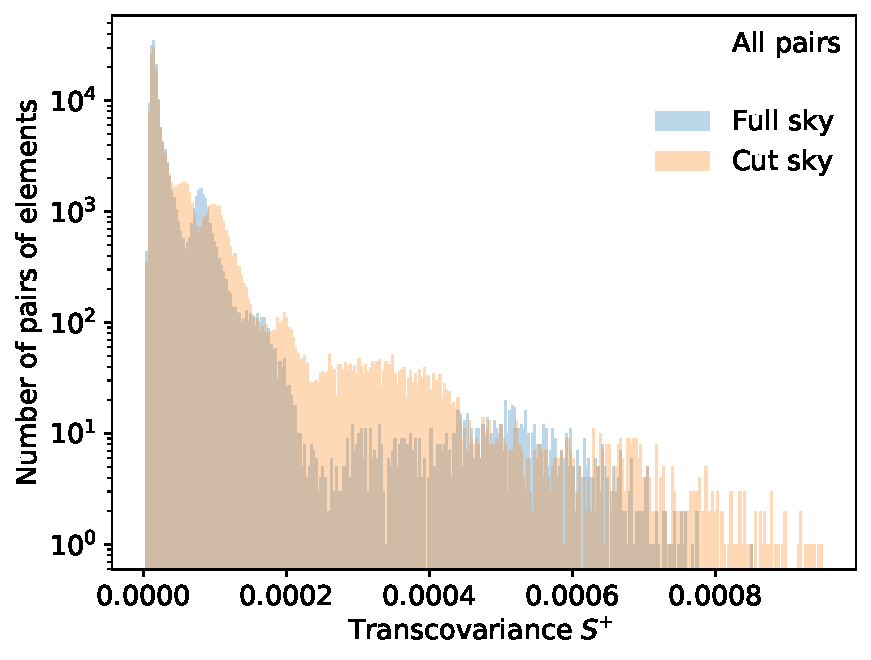
\includegraphics[width=.5\textwidth]{transcov}
\caption{Full-sky and cut-sky distributions of pairwise additive transcovariance after pairwise whitening. Transcovariance is an alternative measure of non-Gaussianity, discussed in \autoref{gl_Sec:transcov}.}
\label{gl_Fig:transcov}
\end{figure}

For completeness, the distributions of additive transcovariance for the full-sky and cut-sky samples are shown in \autoref{gl_Fig:transcov}. There is a much larger excess of transcovariance in the cut-sky likelihood compared to the full-sky likelihood than is seen for the MI in \autoref{gl_Fig:mi_all}. The fact that the transcovariance mixes the effects of non-Gaussian marginals and non-Gaussian dependence would prevent the identification of whether this is due to the marginals, the dependence or both. As an additional check, a probability integral transform was applied to each pair such that the marginal distributions were Gaussian distributed, without affecting the dependence structure, and the resulting distribution had a much smaller cut-sky excess, similar to the MI shown previously in \autoref{gl_Fig:mi_all}.

\section{Non-Gaussian fields}
\label{gl_Sec:nongauss_fields}

It has been demonstrated in \autoref{gl_Sec:fullsky} that a Gaussian likelihood is sufficient to obtain accurate parameter constraints in a combined weak lensing and galaxy clustering analysis on the full sky, and in \autoref{gl_Sec:cut_sky} that the additional non-Gaussianity of the cut-sky likelihood is insufficient to introduce significant inaccuracy, both provided that the observable fields may be described using Gaussian statistics. There are reasons to believe this to be a good approximation for the purposes of this study.

First, the matter distribution is most Gaussian on linear scales, corresponding to low $\ell$, and most non-Gaussian at high $\ell$. But the inverse is true for the power spectrum likelihood: it is most Gaussian at high $\ell$, and most non-Gaussian at low $\ell$. While this behaviour has been demonstrated in the previous sections for Gaussian fields, it can be expected to hold generally, as the number of $\alm$s contributing to each $\Cl$ estimate increases with $\ell$ regardless of the statistics of the field.
The largest contribution to potential inaccuracy in the Gaussian likelihood therefore comes from linear scales, where the observable fields are well described as Gaussian.
Additionally, the presence of shape noise causes two further effects: it decreases the non-Gaussianity of the fields on all scales, and relatively upweights the contribution of large scales to the overall constraining power, as discussed in \autoref{gl_Sec:robustness}. Both of these effects will increase the accuracy of the Gaussian fields assumption.
Finally, the process of going from galaxy catalogues to power estimates involves first averaging over galaxies in each pixel, followed by a spherical harmonic transform, both of which may be expected to approximately Gaussianise the $\alm$s following the central limit theorem.
The latter principle has been tested in simple simulations using \texttt{HEALPix} spherical harmonic transforms of arbitrary non-Gaussian fields and found to hold. Gaussian $\alm$s in turn imply approximately gamma-distributed auto-$\Cl$ estimates. However, the degrees of freedom in these gamma distributions may be reduced (and hence the non-Gaussianity increased) if the $\alm$s are correlated, similar to what happens on the cut sky. This idea was tested in \citet{Taylor2019}, which found no detectable difference between $\Cl$ distributions measured from Gaussian and lognormal simulations, which have been shown to well approximate real weak lensing data \citep{Taruya2002, Hilbert2011, Clerkin2016}.

However, non-Gaussian fields will introduce additional contributions to the $C_\ell$ covariance, which have been neglected here. Specifically, there is a contribution arising from
four-point correlations within a survey volume---often referred to as the connected non-Gaussian covariance---and a generally larger contribution arising from the dependence of such correlations on unmeasured super-survey modes---commonly termed super-sample covariance.
This topic is explored in detail in \autoref{chap:cov}. (See also e.g. \cite{Scoccimarro1999, Cooray2001, Takada2007, Takada2013, Li2014, Barreira2018ssc, Barreira2018b}.)
These additional covariance contributions predominantly affect high $\ell$, which will have the effect of relatively upweighting the low-$\ell$ regime where the Gaussian likelihood is least accurate. However, \autoref{gl_Sec:robustness} showed that the Gaussian likelihood still performs well even at extremely low $\ell$, so we should not expect this to outweigh the other factors outlined above, and
we can expect the overall impact of non-Gaussian fields on the accuracy of a Gaussian likelihood to be negligible. Nevertheless, here the same techniques as in \autoref{gl_Sec:cut_sky} are applied to test the non-Gaussianity detected in a more realistic set of weak lensing simulations.

\subsection{Non-Gaussian fields: Simulations}

The tests presented in this section use the SLICS\footnote{\url{https://slics.roe.ac.uk}}, which are independent N-body weak lensing simulations, described in detail in \citet{Harnois-Deraps2015} and \citet{Harnois-Deraps2018}.
The only available tomographic power spectra were the weak lensing convergence power spectra from the KiDS-450-like setup used in \citet{Hildebrandt2017}.
These are flat-sky linearly-spaced bandpowers for auto-spectra only, produced from 948 independent realisations of $60\,\text{deg}^2$ sky patches.
Here a value of $\lmax = 5000$ is used, in order to include non-linear scales.

An equivalent batch of Gaussian-field simulations were generated using \texttt{pymaster}, the Python implementation of \texttt{NaMaster}\footnote{\url{https://github.com/LSSTDESC/NaMaster}} \citep{Alonso2019}, using a KiDS-450-like setup with four tomographic bins following the specification in Table 1 of \citet{Hildebrandt2017}.

Following the process in \autoref{gl_Sec:cut_sky}, the non-Gaussianity of the marginals and dependence in the distributions from the SLICS is now compared to the Gaussian field sample.

\subsection{Non-Gaussian fields: Effect on marginal distributions}

\begin{figure}
\centering
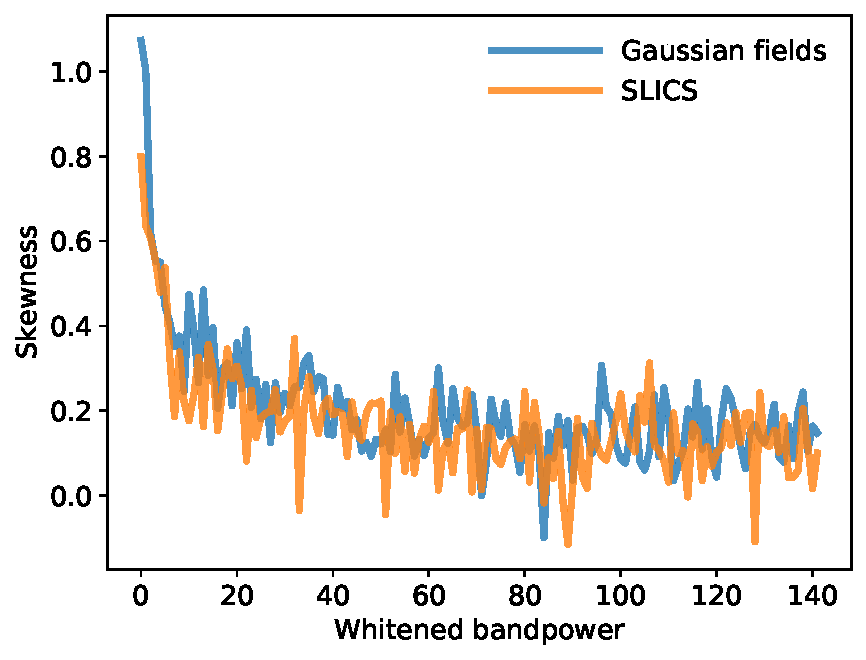
\includegraphics[width=.5\textwidth]{slics_skew}
\caption{Skewness of SLICS bandpowers compared to the Gaussian fields sample, after whitening to remove the effect of linear correlations.}
\label{gl_Fig:slics_skew}
\end{figure}

\autoref{gl_Fig:slics_skew} shows the skewness of the SLICS compared to the Gaussian field sample, averaged over the four redshift bins. Each sample was whitened prior to calculating skewness, because significant linear correlations were found to be present in the SLICS data that were not present in the Gaussian field simulations. These correlations are likely to be real rather than an artefact, since the SLICS were designed and validated specifically for covariance estimation \citep{Harnois-Deraps2015}. However, what matters for the accuracy of a multivariate Gaussian distribution is the non-Gaussianity of the marginals after whitening, since the Gaussian PDF effectively whitens the data vector itself. As shown in \autoref{gl_Fig:slics_skew}, the skewness after whitening is consistent to within the level of the noise, with a possible slight excess for the Gaussian fields. Similar consistency is found for the excess kurtosis. We can therefore conclude that there is no evidence of additional non-Gaussianity of the marginals for realistic non-Gaussian weak lensing fields.

\subsection{Non-Gaussian fields: Effect on dependence structure}

\begin{figure}
\centering
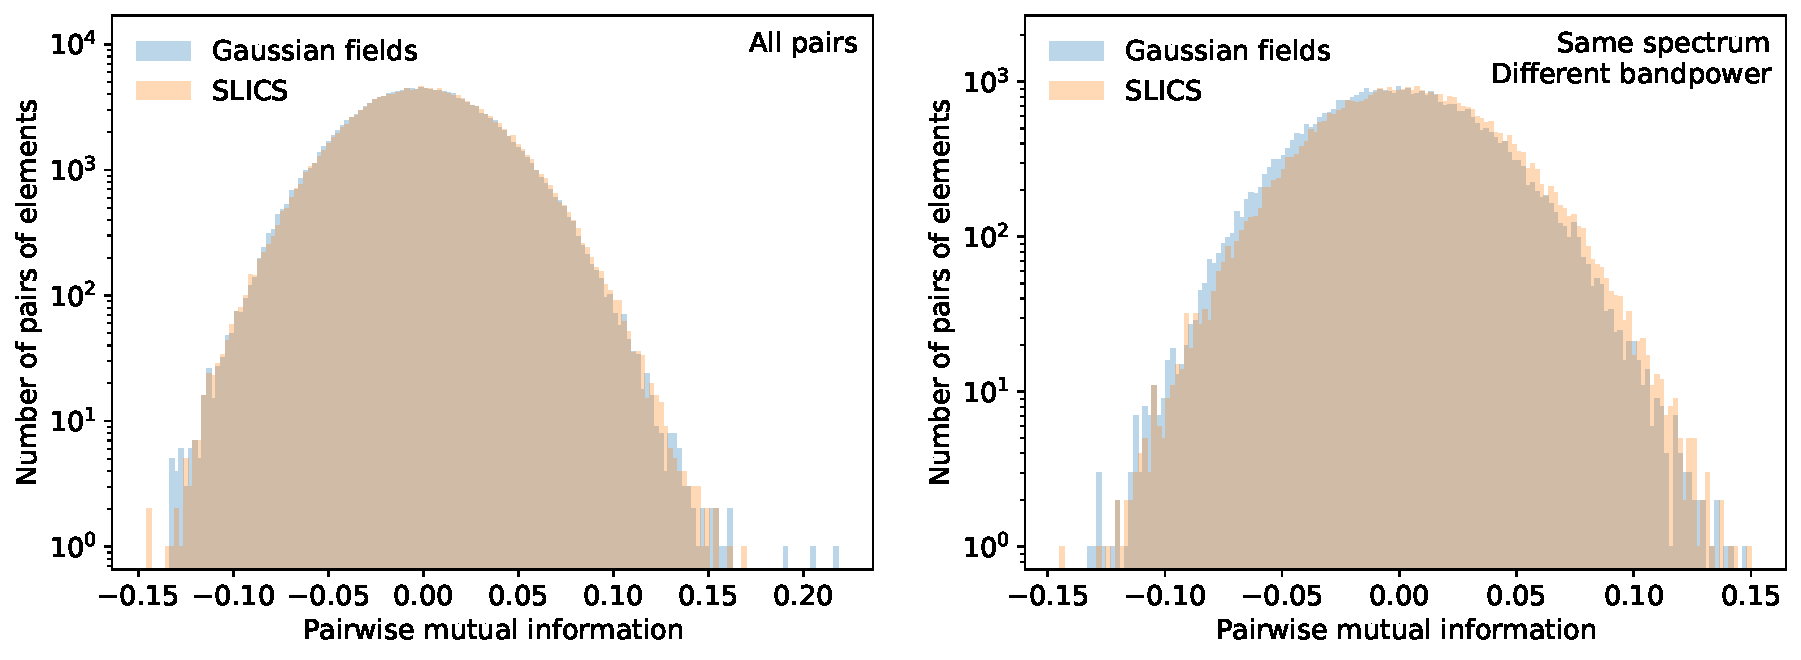
\includegraphics[width=\textwidth]{slics_mi}
\caption{Comparison of non-Gaussian dependence between the SLICS weak lensing simulations and a similar sample of Gaussian fields. Non-Gaussian dependence is quantified by pairwise mutual information after whitening. The left panel shows all pairs of data elements, while the right panel shows only those containing different bandpower pairs in the same spectrum. This population exhibits a possible small excess in non-Gaussian dependence.}
\label{gl_Fig:slics_mi}
\end{figure}

\begin{figure}
\centering
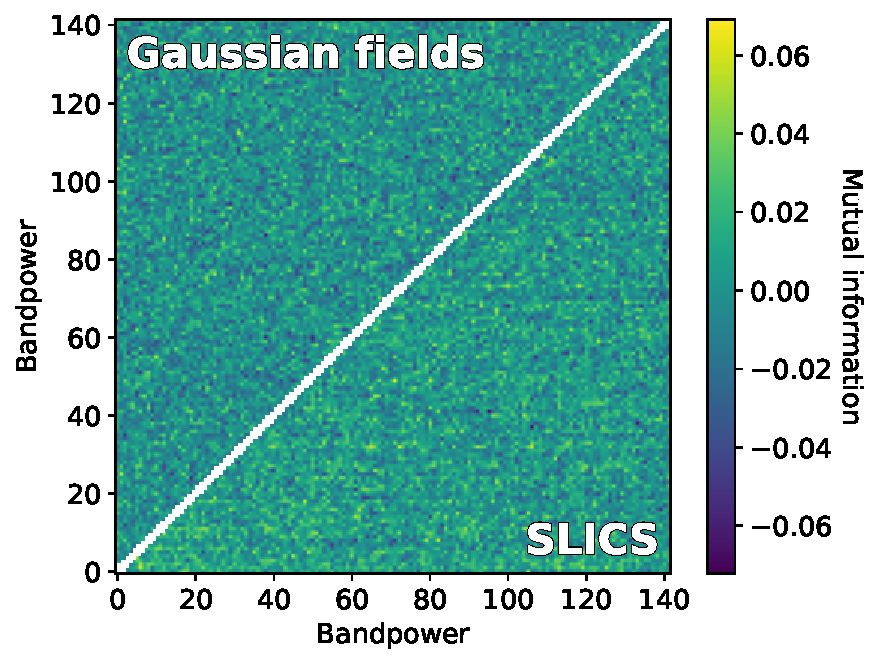
\includegraphics[width=.5\textwidth]{slics_mi_matrix}
\caption{Matrix of pairwise mutual information after pairwise whitening, averaged over four redshift bins, compared between the SLICS and the Gaussian fields sample.}
\label{gl_Fig:slics_mi_matrix}
\end{figure}

Following the procedure described in \autoref{gl_Sec:ma_dependence}, pairwise mutual information (MI) is measured after a pairwise whitening process, and this is compared between the SLICS and the Gaussian field sample.
The overall MI distributions, shown in the left panel of \autoref{gl_Fig:slics_mi}, are almost indistinguishable, but there is a very small excess for the SLICS.
By splitting pairs of data elements into populations depending on their relationship, it is revealed that this excess is due to a particular population: different bandpowers in the same spectrum, shown in the right panel of \autoref{gl_Fig:slics_mi}.
There is no apparent redshift dependence in this behaviour, nor does it have any apparent $\ell$-dependent structure: \autoref{gl_Fig:slics_mi_matrix} shows the matrix of pairwise MI compared between the two samples. Both samples appear consistent with noise, with a slightly higher noise level in the SLICS. Whether this is a real or spurious effect is unknown; however, we can expect its effect on the accuracy of the Gaussian likelihood to be negligible: the average MI for the SLICS is $1.9 \times 10^{-4}$, far below the $9.0 \times 10^{-4}$ that was found to cause negligible inaccuracy in constraints obtained using the Gaussian likelihood in \autoref{gl_Fig:leff_post}. Therefore, no evidence is found to suggest the conclusions drawn from the Gaussian field tests in \autoref{gl_Sec:fullsky} and \autoref{gl_Sec:cut_sky} should not hold for real weak lensing fields.

\section{Conclusions}
\label{gl_Sec:conclusions}

It is well established that the true likelihood of weak lensing two-point statistics is non-Gaussian \citep{Sellentin2018, Sellentin2018a, DiazRivero2020, Louca2020}, and yet contemporary analyses routinely neglect this and assume a Gaussian likelihood \citep{Troxel2018, Hikage2019, Joachimi2021}. The work presented in this chapter has tested the impact of assuming a Gaussian likelihood for a \textit{Euclid}-like combined power spectrum analysis of weak lensing, galaxy clustering and their cross-correlation, on the inferred posterior distributions of dark energy parameters.

In \autoref{gl_Sec:fullsky} it was found that on the full sky, the Gaussian likelihood returns the correct posterior maximum, two-dimensional contours and one-dimensional posterior probability density. This holds both when all other parameters are fixed or when marginalising over a third parameter, and for any choice of fiducial cosmology consistent with the data. The Gaussian likelihood is even a good approximation at low $\ell$, where the true likelihood is most non-Gaussian.

It was shown in \autoref{gl_Sec:cut_sky} that a sky cut increases the non-Gaussianity of both the marginal distributions and dependence structure of the likelihood. However, by generating a mock cut-sky data vector and likelihood with the appropriate amount of non-Gaussianity in both cases, it was shown that this additional non-Gaussianity introduces only negligible additional inaccuracy into the posterior parameter constraints obtained using the Gaussian likelihood.

The results presented in \autoref{gl_Sec:fullsky} and \autoref{gl_Sec:cut_sky} were obtained under the assumption of Gaussian fields. It was argued in \autoref{gl_Sec:nongauss_fields} that this is a sufficient approximation for the purposes of this analysis. Nevertheless, results obtained under this approximation were compared to those obtained using an equivalent set of N-body weak lensing simulations, and no evidence was found of significant additional non-Gaussianity of the power spectrum likelihood.

These results indicate that a Gaussian likelihood will be sufficient for robust cosmological inference with power spectra from stage IV weak lensing surveys such as \textit{Euclid}. This conclusion is further supported by the results obtained in \citet{Taylor2019}, which found no significant difference in parameter constraints obtained using a Gaussian likelihood compared to a likelihood-free approach. We cannot automatically extend this conclusion to the correlation function, which has a more complicated behaviour due to the mixing of scales \citep{Sellentin2018}. \citet{Lin2020} have found that a Gaussian likelihood is likely to be sufficiently accurate for parameter inference from LSST data. However, the disagreement between that result and that of \citet{Hartlap2009}, who found that the assumption of a Gaussian correlation function likelihood introduced significant inaccuracy in parameter constraints from a weak lensing analysis of the Chandra Deep Field South, remains to be fully understood.



% % Uncomment to build alone without subfiles:
% \emergencystretch=.4em % to avoid overfull hboxes
% \printbibliography[heading=bibintoc]
% \end{document}


% % Covariance of weak lensing pseudo-Cl estimates

% % Uncomment to build this alone without subfiles:
% % (also stuff at bottom)
% \documentclass{scrbook}
% % Koma script document options
\KOMAoption{paper}{a4}
\KOMAoption{fontsize}{11pt}
\KOMAoption{parskip}{half-} % paragraph spacing
% \KOMAoption{numbers}{enddot} % dot after section number
\KOMAoption{cleardoublepage}{plain} % include page numbers on blank pages
\KOMAoption{chapterprefix}{true} % 'Chapter' before number

% Packages
\usepackage{amsmath} % Gives \text command inside maths blocks
\usepackage{amssymb} % Various maths symbols
\usepackage{array} % Table formatting
\usepackage{bm} % Bold maths including Greek
\usepackage[format=plain]{caption} % Font sizing and alignment in captions
\usepackage{enumitem} % Allows numbering like 1.1 in ordered lists
% \usepackage{float} % Allows H placement of floats
\usepackage{graphicx}
\usepackage[hidelinks]{hyperref} % Hyperlinks without looking like it
% \usepackage{longtable} % Multi-page tables
% \usepackage{multicol} % For columns in text (not tables)
\usepackage{multirow} % For tables
\usepackage{neuralnetwork} % Neural net diagram
\usepackage{pdflscape} % Gives landscape environment
% \usepackage{scrlayer-scrpage} % To move page numbers
\usepackage{tabularx}
\usepackage{textcomp} % Added to fix \textasciiacute error on laptop
% \usepackage{tikz} % Diagrams (used for neural network example)
% \usepackage[pagenumberwidth=3em]{tocbasic}
% \usepackage{tocstyle} % ToC styling
\usepackage{upgreek} % Non-italic greek letters
\usepackage{xpatch} % Biblatex customisation

\usepackage[a4paper, inner=40mm, outer=15mm, top=30mm, bottom=30mm,footskip=15mm, headsep=15mm]{geometry}
% \usepackage[a4paper, inner=40mm, outer=30mm, top=50mm, bottom=50mm,footskip=20mm, headsep=20mm]{geometry} % footskip is space between footer (i.e. page number) and bottom of text
% min allowed is inner 40 mm, others 15 mm

\pagestyle{plain} % no header for front matter, overridden at end of front matter

% Caption setup
% \tablecaptionabove
\captionsetup[table]{labelsep=space}
% \captionsetup[table]{labelsep=space, skip=50pt, position=top}
\captionsetup[figure]{labelsep=space} % labelsep prevents dot followed by colon in captions

% Line spacing
\usepackage{setspace}
% \setstretch{1.4} % strangely this is > \onehalfspacing but < \doublespacing
\onehalfspacing
% \doublespacing

\raggedbottom % prevent huge spaces between paragraphs

% % % % % % % % % % % % % % % % % % % % % % % % %
% Font setup
% \usepackage{mathpazo} % Covers maths mode too
\usepackage[sc]{mathpazo} % Covers maths mode too, sc enables small caps
% \usepackage{palatino}
\usepackage[T1]{fontenc} % 8-bit font encoding
\addtokomafont{disposition}{\rmfamily} % Use serif throughout
% % % % % % % % % % % % % % % % % % % % % % % % %

% % % % % % % % % % % % % % % % % % % % % % % % %
% Section formatting setup
% \RedeclareSectionCommand[beforeskip=0pt]{chapter}
\RedeclareSectionCommand[beforeskip=0pt, innerskip=0pt]{chapter}
\RedeclareSectionCommand[beforeskip=10pt]{subsubsection}
\RedeclareSectionCommand[afterskip=1pt]{subsubsection}
% \setcounter{secnumdepth}{\subsubsectionnumdepth} % number up to subsubsections

% No dot after chapter number (https://tex.stackexchange.com/a/484727)
\renewcommand*{\chapterformat}{%
  \mbox{\chapappifchapterprefix{\nobreakspace}\thechapter
  \IfUsePrefixLine{}{\enskip}}%
}

% In the running header, separate chapter number and name with em dash
\renewcommand*{\chaptermarkformat}{%
\chapapp~\thechapter~---~}

% Create subsubsubsection below subsubsection but above paragraph, following https://tex.stackexchange.com/a/356574

\DeclareNewSectionCommand[
  style=section,
  counterwithin=subsubsection,
  afterskip=1pt,
  beforeskip=10pt,
  % afterskip=1.5ex plus .2ex,
  % beforeskip=3.25ex plus 1ex minus .2ex,
  % afterindent=false,
  level=\paragraphnumdepth,
  tocindent=10em,
  tocnumwidth=5em
]{subsubsubsection}
\setcounter{secnumdepth}{\subsubsubsectionnumdepth}
% \setcounter{tocdepth}{\subparagraphtocdepth}
\setcounter{tocdepth}{\subsubsubsectionnumdepth}

\RedeclareSectionCommands[
  level=\numexpr\subsubsubsectionnumdepth+1\relax,
  toclevel=\numexpr\subsubsubsectiontocdepth+1\relax,
  increaselevel,
]{paragraph,subparagraph}
\RedeclareSectionCommand[
  counterwithin=subsubsubsection,
  tocindent=12em,
  tocnumwidth=6em,
  beforeskip=10pt,
  afterskip=1pt, % line break after paragraph title
]{paragraph}
\RedeclareSectionCommand[
  tocindent=14em,
  tocnumwidth=7em,
  beforeskip=0pt
]{subparagraph}
% % % % % % % % % % % % % % % % % % % % % % % % %

% Autoref capitalisation
\def\chapterautorefname{Chapter}
\def\sectionautorefname{Section}
\def\subsectionautorefname{Section}
\def\subsubsectionautorefname{Section}

% % % % % % % % % % % % % % % % % % % % % % % % %
% Bibliography setup
\usepackage[backend=biber,
    % style=authoryear,
    style=authoryear-comp, % Don't repeat same author(s) in multiple citations
    giveninits=true,
    useprefix=true, % 'van der' etc.
    url=false,
    doi=false,
    isbn=false,
    eprint=false,
    uniquename=false, % Don't add initials in citation to disambiguate between authors with the same surname
    uniquelist=false, % Don't disambiguate in citation between different 'et al.' teams
    maxbibnames=10,
    minbibnames=10,
    maxcitenames=3,%  # 2,
    natbib, % Gives citep and citet commands
    labelalpha=true, % Use an 'alpha' label for each bib entry
    maxalphanames=1, % Use first author as the alpha label
    sorting=anyvt, % Sort by alpha (first author) then year
    block=par, % New line between 'blocks' of the bib entry
    dashed=false, % Reprint author list for each publication in bibliography
    sortcites=false % Show citations in the order supplied
]{biblatex}

% Citation/reference parameters
\renewcommand*{\nameyeardelim}{\addspace} % Space between author and year rather than comma
\renewcommand*{\finalnamedelim}{\addspace\&\addspace} % Ampersand rather than 'and'
\xpatchbibmacro{name:andothers}{{\finalandcomma}}{\addspace}{}{} % Space before 'et al.' rather than comma

% Citation-specific parameters
\DeclareCiteCommand{\blindcite}{\unspace}{}{}{\mancite} % Easy manual citations

% Reference-specific parameters
\AtEveryBibitem{\clearfield{title}} % Suppress title
\AtEveryBibitem{\clearfield{month}} % Suppress month
\DeclareNameAlias{author}{family-given} % Surname first for not just the first author
\DeclareNameAlias{editor}{family-given} % Same for editors
\renewbibmacro{in:}{} % Remove 'In:'
\DeclareFieldFormat{journaltitle}{#1} % Journal title in normal font rather than italics
\renewbibmacro*{volume+number+eid}{\printfield{volume}\printfield{number}\setunit{\addcomma\space}\printfield{eid}} % No dot after issue
\DeclareFieldFormat[article]{number}{\mkbibparens{#1}} % Volume in brackets
\DefineBibliographyStrings{english}{page = {}, pages = {}} % Suppress 'p.'/'pp.'
\renewbibmacro*{date+extradate}{\printtext{\printfield{year}\addcomma}} % Year not in brackets
\DeclareFieldFormat{pages}{\mkfirstpage[{\mkpageprefix[bookpagination]}]{#1}} % Only give starting page
\DeclareFieldFormat{url}{\url{#1}} % No 'URL' before URLs
% \renewcommand{\finentrypunct}{} % Remove final full stop
\renewcommand*{\newunitpunct}{\addcomma\space} % Commas between elements of bibitems

\DeclareBibliographyDriver{book}{%
  \printnames{author}%
  \space
  \printfield{year}%
  \newunit\newblock
  \printfield{booktitle}%
  \newunit
  , \printlist{publisher}%
\finentry}

\DeclareBibliographyDriver{inproceedings}{%
  \printnames{author}%
  \space
  \printfield{year}%
  \newunit\newblock
  \printfield{booktitle}%
  \newunit
  \printfield{volume}%
  \newunit
  \printfield{pages}%
\finentry}

\DeclareBibliographyDriver{incollection}{%
  \printnames{author}%
  \space
  \printfield{year}%
  \newunit\newblock
  \printfield{booktitle}%
  \newunit
  , ed. \printnames{editor},%
  \newunit\newblock
  \printlist{publisher}%
\finentry}

\DeclareBibliographyDriver{misc}{%
  \printnames{author}%
  \space
  \printfield{year}%
  \newunit\newblock
  \printfield{title}%
  \newunit
  \printfield{url}%
\finentry}

\addbibresource{refs.bib}
% % % % % % % % % % % % % % % % % % % % % % % % %

% Footnote spacing
% \deffootnote[1em]{1.5em}{1em}{\textsuperscript{\thefootnotemark~}}
\deffootnote[1em]{1em}{1em}{\textsuperscript{\thefootnotemark~}}

% Testing setting all penalties to zero
\binoppenalty=0
\brokenpenalty=0
\clubpenalty=0
\displaywidowpenalty=0
\exhyphenpenalty=0
\floatingpenalty=0
\hyphenpenalty=0
\interlinepenalty=0
% \linepenalty=0 % allowing this to be zero splits titles in a strange way
\postdisplaypenalty=0
\predisplaypenalty=0
\relpenalty=0
\widowpenalty=0

% Shorthands (non-Maths)
\newcommand{\lcdm}{$\Lambda$CDM}
\newcommand{\wcdm}{$w$CDM}
\newcommand{\Euclid}{\textit{Euclid}}
\newcommand{\Planck}{\textit{Planck}}
\newcommand{\Pcl}{Pseudo-$C_\ell$}
\newcommand{\pcl}{pseudo-$C_\ell$}
\newcommand{\ttp}{3$\times$2\,pt}

% Maths shorthands
\newcommand{\alm}{a_{\ell m}}
\newcommand{\Cl}{C_\ell}
\newcommand{\fsky}{f_\text{sky}}
\newcommand{\lmax}{\ell_\text{max}}
\newcommand{\lmin}{\ell_\text{min}}
\newcommand{\leff}{\ell_\text{eff}}
\newcommand{\tmin}{\theta_\text{min}}
\newcommand{\mathbfit}[1]{\bm{\mathit{#1}}}
\newcommand{\mathbfss}[1]{\bm{\mathsf{#1}}} % to match MNRAS \mathbfss
\renewcommand{\Re}{\operatorname{Re}}
\renewcommand{\Im}{\operatorname{Im}}

% ΛCDM parameters (maths mode)
\newcommand{\wo}{w_0}
\newcommand{\wa}{w_a}
\newcommand{\omm}{\Omega_\text{m}}
\newcommand{\omb}{\Omega_\text{b}}
\newcommand{\omc}{\Omega_\text{c}}
\newcommand{\sie}{\sigma_8}

% % Editing only
% \usepackage{xcolor}
% \newcommand{\todo}[1]{\textbf{{\color{red}{#1}}}}


% \usepackage{subfiles} % Best to do this last apparently

% \pagestyle{headings}
% \setcounter{chapter}{4} % deliberately 1 too low
% \begin{document}

% Uncomment to use subfiles:
% \documentclass[../Thesis.tex]{subfiles}
% \begin{document}

\chapter{Covariance of weak lensing pseudo-\texorpdfstring{$C_\ell$}{Cl} estimates}
\label{chap:cov}
\graphicspath{{../Figs/cov/}{Figs/cov/}}

\section{Introduction}

There are currently many unanswered questions in cosmology, including the origin of the accelerating expansion of the Universe and apparent tensions within the dominant \lcdm{} model. As described in \autoref{chap:cosmo}, one of the most promising tools with which to make progress on these questions in the coming years is the analysis of weak gravitational lensing of distant galaxies by large-scale structure, also known as cosmic shear.
The upcoming ESA \Euclid{} space mission, as well as other surveys such as those with the Vera C. Rubin Observatory in Chile and the Square Kilometre Array radio observatory in Australia and South Africa,
will observe over a billion galaxies, which is expected to lead to unprecedented precision on cosmological constraints---a more than an order of magnitude increase over the previous generation of experiments \citep{Harrison2016}. In order to obtain reliable results, this precision is necessarily accompanied by a requirement to understand all elements of an analysis pipeline to an equally unprecedented degree, including the interplay between the likelihood and estimator effects.

Continuing from Chapters \ref{chap:exact_like} and \ref{chap:gauss_like}, this chapter is concerned specifically with pseudo-$C_\ell$ estimators, which were introduced in \autoref{chap:est_like}. \Pcl{} estimators have been used previously for the analysis of weak lensing data from the Hyper-Suprime Cam Subaru Strategic Program in \citet{Hikage2019} and the Dark Energy Survey (DES) in \citet{Camacho2021} and will be used in the analysis of future \Euclid{} data \citep{Loureiro2021}. It was shown in \autoref{chap:gauss_like} that a Gaussian likelihood is sufficient to obtain accurate cosmological results from weak lensing pseudo-$C_\ell$ estimates. An important ingredient for a Gaussian likelihood is the covariance matrix, so this chapter focuses on the calculation of a cosmic shear pseudo-$C_\ell$ covariance matrix.

The problem of calculating covariance matrices for weak lensing has been extensively discussed in the literature, ranging from analytic or semi-analytic approaches \citep{Cooray2001, Schneider2002, Joachimi2008cov, Takada2009, Pielorz2010, Hilbert2011, Barreira2018ssc, Hall2019, GouyouBeauchamps2021} through to estimation from simulations \citep{Sato2011, Harnois-Deraps2015, Sellentin2016, Sellentin2016b, Harnois-Deraps2018, Harnois-Deraps2019, Sgier2019, Schneider2020}. This chapter extends this work to focus specifically on the covariance of pseudo-$C_\ell$ estimates, for which coupling between modes occurs due to the effect of incomplete sky coverage. This effect is in addition to the non-Gaussian mode coupling that is inherent in weak lensing data as a result of non-linear structure growth, and which is known to be important for parameter inference \citep{Sato2013, Barreira2018b}.

In \autoref{cov_sec:theory} the different Gaussian and non-Gaussian components of the cosmic shear pseudo-$C_\ell$ covariance and their implementation in existing publicly available code are described.
This theoretical covariance is compared to that measured from publicly available weak lensing simulations in \autoref{cov_sec:sims}.
\autoref{cov_sec:importance} examines the relative importance of the different covariance contributions and how this depends on the mask, which describes the details of sky coverage.
This part of the analysis shares some similarities with that of \citet{Barreira2018b}, who also studied the relative importance of the different contributions to the cosmic shear covariance for a \Euclid{}-like survey and concluded that the `connected non-Gaussian' component (see \autoref{cov_sec:theory}) can be neglected for only a $\lesssim$ 5 per cent underestimation in single-parameter 1$\sigma$ errors.
However, this chapter is specifically focused on pseudo-$C_\ell$ estimates, for which the survey mask mixes power between all multipoles and induces correlations even for Gaussian fields, which for many covariance elements dominate over other sources of correlation (see \autoref{cov_sec:sims}).
This effect was not included in the analysis of \citet{Barreira2018b}, who assumed a diagonal Gaussian covariance, and its inclusion may lead to different conclusions about the relative importance of the different contributions to the covariance.
The conclusions of this work are discussed in \autoref{cov_sec:conclusions}.

\section{Cosmic shear power spectrum covariance contributions}
\label{cov_sec:theory}

There are three contributions to the cosmic shear power spectrum covariance, which are summarised below. A thorough theoretical background and derivation may be found in \citet{Barreira2018ssc} and the other references provided both therein and below.

Starting in three-dimensional space, the covariance of the matter power spectrum receives two contributions: one that depends on the matter power spectrum itself, and one that depends on a particular (`parallelogram') configuration of the matter trispectrum that corresponds to the Fourier transform of the connected four-point correlation function. For a Gaussian matter distribution, only the first contribution is non-vanishing, and hence it is commonly referred to as the `Gaussian covariance', which will be used in this chapter. (It is also sometimes referred to as the `disconnected' covariance.) Following \citet{Barreira2018ssc}, the second contribution is referred to as the `connected non-Gaussian' component.

However, for any realistic finite-volume survey such as \Euclid{}, the observed matter power spectrum is convolved with a three-dimensional window function. While the Gaussian and non-Gaussian terms remain distinct, this has the effect of introducing additional non-Gaussian coupling between large-scale modes outside the survey and small-scale modes within the survey. This is commonly known as `super-sample' (originally `beat-coupling'; \citealt{Hamilton2006}) covariance, and physically can be explained by the fact that unobservable large-scale modes within which the survey is embedded can influence the rate of small-scale non-linear structure growth, and therefore also the strength of coupling between small-scale modes \citep{Takada2013, Barreira2018ssc}. Perhaps counter-intuitively, it turns out that this is generally the dominant source of non-Gaussian covariance \citep{Hamilton2006, Barreira2018b}.

Progressing to projected two-point statistics such as cosmic shear angular power spectra, the same three components---Gaussian, super-sample and connected non-Gaussian---contribute to the covariance. Strictly speaking, the separation of the super-sample and connected non-Gaussian components is only exact under the Limber approximation \citep{Barreira2018ssc}, but the inaccuracy of the Limber approximation is only relevant on very large scales (very low multipoles, $\ell \lesssim 20$) where non-Gaussian correlations are small.

The calculation of the three cosmic shear covariance components are each now discussed in turn.

\subsection{Gaussian covariance}

To calculate the Gaussian covariance, the `improved narrow kernel approximation' method \citep{Nicola2021} was used, which was implemented using the publicly available code \texttt{NaMaster} \citep{Alonso2019, Garcia-Garcia2019}. Further details and some background on this method are provided as follows.

The Gaussian covariance component of a general statistically isotropic field on the sphere is equivalent to the total covariance of a Gaussian field with the same power spectrum. The analytic covariance of pseudo-$C_\ell$ estimates on Gaussian fields has been well studied in the cosmic microwave background literature \citep{Efstathiou2004, Challinor2005, Brown2005} as well as in the context of weak lensing \citep{Garcia-Garcia2019, Nicola2021}. The exact Gaussian pseudo-$C_\ell$ covariance can be written down analytically, and includes terms of the following form \citep[e.g.][]{Brown2005}:
\begin{equation}
\begin{aligned}
\text{Cov} \Big( \widetilde{C}_\ell,~ \widetilde{C}_{\ell'} \Big) =
&\sum_{\substack{m,~m'\\\ell_1,~\ell_2\\m_1,~m_2}}
W_{\ell \ell_1}^{m m_1} \left( W_{\ell' \ell_1}^{m' m_1} \right)^*
W_{\ell' \ell_2}^{m' m_2} \left( W_{\ell \ell_2}^{m m_2} \right)^*
C_{\ell_1} C_{\ell_2} \\
&+ \text{similar terms},
\end{aligned}
\label{cov_eqn:pcl_cov}
\end{equation}
where the harmonic space window functions $W$ are given in Equation (8) of \citet{Brown2005}, and the `similar terms' involve different combinations of power spectra depending on the situation and spins being considered \citep{Hansen2003, Challinor2005}.

The evaluation of Equation \eqref{cov_eqn:pcl_cov} requires $\mathcal{O}(\ell_\text{max}^6)$ operations per term, so it is impractical to evaluate exactly and in practice approximations are used. These commonly involve substitutions of the following kind \citep{Efstathiou2004,Brown2005,Garcia-Garcia2019}:
\begin{equation}
C_{\ell_1} C_{\ell_2} \rightarrow C_\ell C_{\ell'},
\label{cov_eqn:nka}
\end{equation}
which allows the power spectrum dependence to be brought out of the sums in Equation \eqref{cov_eqn:pcl_cov}. This means that the coefficients in the similar terms are now all the same (except for any possible spin dependence, or if different fields use different masks). Symmetry properties of the harmonic space window function allow the calculation of these coefficients to be further simplified, to the point where the covariance can be evaluated in a reasonable time. In essence, the approximation in Equation \eqref{cov_eqn:nka} assumes that the power spectrum is constant over the region around a given $\ell$ in which the window function is non-negligible. This will be accurate as long as the window function is sufficiently sharply peaked, and therefore this approximation is often known as the `narrow kernel approximation' (NKA).
A generalised version of the NKA is described in \citet{Garcia-Garcia2019} and implemented in \texttt{NaMaster}, which supports an arbitrary number of correlated spin-0 and spin-2 fields and has both curved-sky and flat-sky support. For this work the curved-sky spin-2 version was used, which naturally accounts for $E$--$B$ leakage (here assuming noise-only $B$-modes). By default, \texttt{NaMaster} provides the covariance of deconvolved pseudo-$C_\ell$ estimates, but here the \texttt{coupled=True} option is set to instead obtain the covariance of `raw', un-deconvolved estimates such as those produced by the pseudo-$C_\ell$ estimator developed for \Euclid{}, which is described in \citet{Loureiro2021}. No $E$--$B$ purification or noise de-biasing was applied.

\citet{Nicola2021} introduced a small modification to the NKA that turns out to significantly increase its accuracy, which they refer to as the improved NKA. It involves simply replacing each $C_\ell$ in the standard NKA by its mode-coupled counterpart,
\begin{equation}
C_\ell \rightarrow
\frac{\langle \widetilde{C}_\ell \rangle}{f_\text{sky}}
= \frac{\sum_{\ell'}
\mathbfss{M}_{\ell \ell'}
C_{\ell'}}{f_\text{sky}},
\end{equation}
where
$\mathbfss{M}$
is the usual pseudo-$C_\ell$ mixing or mode-coupling matrix (see \citealt{Brown2005} for a full derivation of its calculation), and the division by the sky fraction $f_\text{sky}$ is to avoid double-counting the loss of power on the cut sky. \texttt{NaMaster} includes the functionality to calculate the mixing matrix and to apply it to power spectra to calculate $\langle \widetilde{C}_\ell \rangle$, so the extension to the improved NKA is trivial. The recent pseudo-$C_\ell$ analysis of DES Year 1 observations in \citet{Camacho2021} provided the first application of the improved NKA to real data, but takes the approach of deconvolution and noise subtraction to obtain unbiased estimates of the underlying power spectrum, unlike the forward-modelling approach taken in this chapter.

\subsection{Super-sample covariance}
\label{cov_sec:ssc}

To calculate the super-sample covariance contribution, the publicly available code \texttt{Cosmo-} \texttt{Like}\footnote{\url{https://github.com/CosmoLike}} \citep{Krause2017CosmoLike} was used;
specifically,
an adapted version of the \texttt{CosmoCov}\footnote{\url{https://github.com/CosmoLike/CosmoCov}} correlation function covariance package \citep{Fang2020CosmoCov}, which obtains the real-space non-Gaussian covariance as a transform of the harmonic space covariance. \texttt{CosmoCov} has been used for the DES Year 1 and Year 3 cosmological analyses \citep{Krause2017, Krause2021, Friedrich2021}, as well as for the non-Gaussian covariance in the Year 1 pseudo-$C_\ell$ analysis in \citet{Camacho2021}.
The code adapted for this work to expose the harmonic space covariance directly is available online.\footnote{\url{https://github.com/robinupham/CosmoCov_ClCov}}

\texttt{CosmoLike} calculates the super-sample covariance using the approach introduced in \citet{Takada2013}, by considering the response of the small-scale non-linear matter power spectrum to changes in the mean linear density field \citep[see also][]{Chiang2014,Li2014}. The response of the non-linear matter power spectrum is evaluated using a halo model, with the details given in Equations (A7)--(A11) of \citet{Krause2017CosmoLike}. Since that paper was published, the calculation of the survey variance $\sigma_b (z)$ in their Equation (A8) has been replaced within \texttt{CosmoLike} with the following calculation:
\begin{equation}
\sigma_b \left( z \right) = \frac{1}{4 \pi r^2}
\frac{1}{C_{\ell = 0}^\text{mask}}
\sum_{\ell = 0}^{1000}
\left( 2 \ell + 1 \right) \, C_\ell^\text{mask} \,
P_\text{lin} \left( \frac{\ell + 1/2}{r}, \, z \right),
\label{cov_eqn:survey_variance}
\end{equation}
where $r = f_\kappa \left( \chi \left( z \right) \right)$, and $C_\ell^\text{mask}$ is the power spectrum of the mask.
This treatment of the cut sky using the mask power spectrum was derived in \citet{Barreira2018ssc}.
The value of $\ell_\text{max} = 1000$ in Equation \eqref{cov_eqn:survey_variance} is arbitrary, but has a negligible impact in practice because the power spectrum of both masks is negligible above $\ell \sim 100$.
\texttt{CosmoLike} also provides an alternative implementation of both the super-sample and connected non-Gaussian covariance using the `response approach', which additionally accounts for a tidal contribution to the super-sample covariance and has been found to be more accurate than the standard implementation \citep{Wagner2015, Barreira2017a, Barreira2017b, Barreira2018ssc, Schmidt2018}. Here the standard \texttt{CosmoLike} implementation is used, as has been used by the DES Collaboration \citep{Krause2017, Krause2021, Friedrich2021, Camacho2021}.

As stated previously, the approach taken in this work is to forward-model the effect of the mask to obtain the covariance of raw un-deconvolved pseudo-$C_\ell$ estimates following \citet{Loureiro2021}.
The non-Gaussian covariance output from \texttt{CosmoLike} corresponds to the covariance of unbiased estimates of the underlying power spectrum $\widehat{C}_\ell$, and does not account for any estimator effects such as cut-sky mode coupling. Within the context of the pseudo-$C_\ell$ method, the closest way to interpret the covariance output from \texttt{CosmoLike} is as the covariance of deconvolved pseudo-$C_\ell$ estimates. This is how it is interpreted in \citet{Camacho2021}, and how it is interpreted in this work. In this case, the unbiased estimates $\widehat{C}_\ell$ may in principle be obtained from raw pseudo-$C_\ell$ estimates $\widetilde{C}_\ell$ as
\begin{equation}
\widehat{C}_\ell = \sum_{\ell'} \mathbfss{M}^{-1}_{\ell \ell'} \widetilde{C}_{\ell'}.
\end{equation}
It follows that the covariance matrices of $\widehat{C}_\ell$ and $\widetilde{C}_\ell$, denoted respectively here as $\mathbf{\widehat{\Sigma}}$ and $\mathbf{\widetilde{\Sigma}}$, are related as
\begin{equation}
\mathbf{\widehat{\Sigma}} =
\left( \mathbfss{M}^{-1} \right)
\mathbf{\widetilde{\Sigma}}
\left( \mathbfss{M}^{-1} \right)^\intercal.
\label{cov_eqn:cov_transform_inverse}
\end{equation}
The covariance as output from \texttt{CosmoLike} is interpreted as $\mathbf{\widehat{\Sigma}}$.
This choice is necessarily an approximation since \texttt{CosmoLike} does not account for any estimator effects, including pseudo-$C_\ell$ mode coupling, but it is a necessary choice and is equivalent to that made in the DES Y1 pseudo-$C_\ell$ analysis in \citet{Camacho2021}. In both that paper and this work (\autoref{cov_sec:sims}), the resulting covariance is compared to simulations, with good agreement. A full general non-Gaussian pseudo-$C_\ell$ covariance is presented in \citet{Shirasaki2015}, but in practice an approximation such as the one made here is necessary.
Equation \eqref{cov_eqn:cov_transform_inverse} is therefore inverted to obtain the relation that was used to transform $\mathbf{\widehat{\Sigma}}$ to the raw pseudo-$C_\ell$ covariance, $\mathbf{\widetilde{\Sigma}}$:
\begin{equation}
\mathbf{\widetilde{\Sigma}} =
\mathbfss{M} \mathbf{\widehat{\Sigma}} \mathbfss{M}^\intercal.
\label{cov_eqn:cov_transform}
\end{equation}
The spin-2 mixing matrix \mathbfss{M} for this calculation was obtained using \texttt{NaMaster}.

\subsection{Connected non-Gaussian covariance}

The connected non-Gaussian covariance component was also calculated using \texttt{CosmoLike} (referred to in \citealt{Krause2017CosmoLike} as the `non-Gaussian covariance in the absence of survey window effects'), using the same adapted version of the \texttt{CosmoCov} package that is made available at the URL provided in \autoref{cov_sec:ssc}.

\texttt{CosmoLike} calculates the connected non-Gaussian covariance as the projected matter tri- spectrum. The trispectrum is calculated using a halo model, with the details given in Equations (A3)--(A6) of \citet{Krause2017CosmoLike} \citep[see also][]{Cooray2002, Takada2009}.
This is found to be suitably accurate in \autoref{cov_sec:cov_vs_sims}, and it is also shown in \autoref{cov_sec:importance} that the contribution from the connected non-Gaussian component to the total parameter posterior error is no more than 10--20 per cent.
As with the super-sample covariance component, the connected non-Gaussian covariance matrix was multiplied by the mixing matrix using Equation \eqref{cov_eqn:cov_transform}.

The calculation of the connected non-Gaussian covariance component is much slower than the other two components.
As a result, in \autoref{cov_sec:params} an approximation is used to directly estimate the connected non-Gaussian covariance of power spectrum bandpowers (i.e. power spectra that have been binned in multipole space), which are subsequently used to obtain mock parameter constraints. The approximation is described in that section.
However, the results provided in Sections \ref{cov_sec:sims} and \ref{cov_sec:rel_sizes} were obtained using the full (i.e. per-multipole) connected non-Gaussian covariance matrix for a single redshift bin. This took 36 days to calculate on 55 CPUs for 32 million elements.\footnote{This number comes from a data vector running from $\ell_\text{min} = 2$ to $\ell_\text{min} = 8000$, which has a length of $n = 8000 - 2 + 1 = 7999$, leading to a number of unique covariance elements equal to $n \left( n + 1 \right) / 2 = 31\,996\,000$.} By contrast, the equivalent Gaussian and super-sample covariance matrices each took around an hour to calculate on 12 CPUs.

\section{Comparison to simulations}
\label{cov_sec:sims}

\subsection{Method}

The publicly available\footnote{\url{http://cosmo.phys.hirosaki-u.ac.jp/takahasi/allsky_raytracing}} full-sky simulated spin-2 shear maps of \citet{Takahashi2017} were used, which were produced by ray tracing through cosmological N-body simulations. The simulations use a maximum box size of $6300 \, h^{-1} \text{Mpc}$. These simulated maps are quite versatile, not only because they cover the full sky, but also because they describe the underlying shear field with no shape noise or shot noise (which could be added if required, but is not added for this work). A total of 108 realisations were performed, which is a relatively small number considering that very large numbers of realisations may be required for full convergence of a simulated covariance \citep{Blot2016}, but the results show that a useful comparison between theory and simulations is still possible. In addition, finite box simulations will necessarily underestimate the super-sample covariance \citep{Hamilton2006, Li2014}, but a significant deficit is not detected. Further details and validation of the simulations can be found in \citet{Takahashi2017}, and density maps, halo catalogues and lensed cosmic microwave background maps are also available at the same URL.

The shear maps are provided at 38 redshift slices from $z = 0.05$ to 5.3.
For each realisation, these were combined into five redshift bins, following a Gaussian redshift distribution centred at $z = 0.65$, 0.95, 1.25, 1.55, 1.85 with a standard deviation of 0.3.
The combined shear map for each redshift bin was formed as a weighted average over all 38 slices, with the weights given by the probability density of a Gaussian distribution with the appropriate mean and standard deviation. This choice of redshift distribution is discussed below, in \autoref{cov_sec:redshift}.
Three copies were then taken: one full-sky with no mask, one with a full \Euclid{}-like mask including the survey footprint and a bright star mask ($f_\text{sky} = 0.31$), and one with a \Euclid{} DR1-like footprint but no bright star mask ($f_\text{sky} = 0.06$). The full \Euclid{}-like and \Euclid{} DR1-like masks are shown in \autoref{cov_fig:masks}. These masks approximate the coverage of the Euclid Wide Survey at different stages but do not exactly correspond to what will be observed, which is described in \citet{Scaramella2021}. It is also assumed that the masks are uncorrelated with the signal, which may not be the case in practice \citep[e.g.][]{Fabbian2021}. Finally, the \texttt{healpy} \citep{Zonca2019} interface to the \texttt{HEALPix} \citep{Gorski2005} software was used to measure the spin-2 shear power spectra for each realisation. The comparisons shown in this section are for the $E$-mode auto-power in the lowest redshift bin.

\begin{figure}
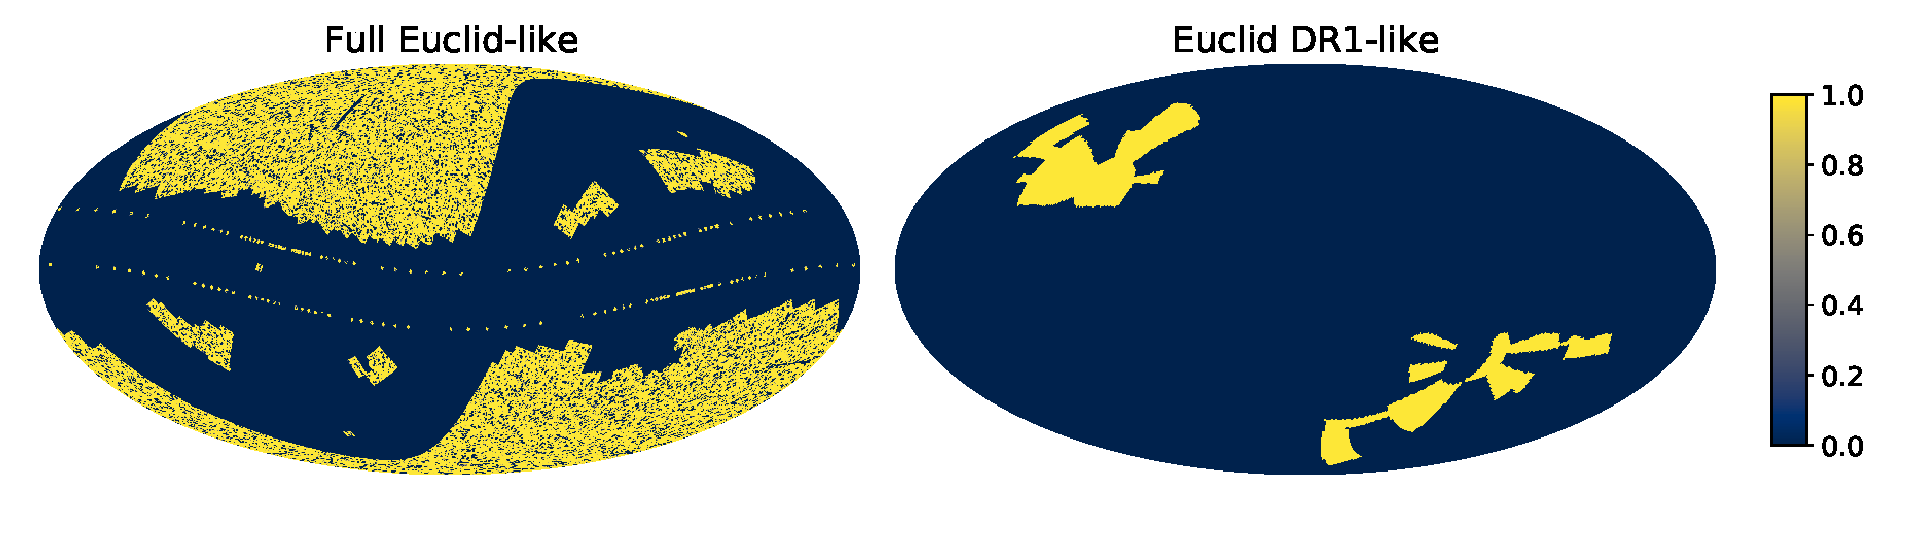
\includegraphics[width=\textwidth]{masks}
\caption{Full \Euclid{}-like and \Euclid{} DR1-like masks, which are used in Sections \ref{cov_sec:sims} and \ref{cov_sec:importance} to quantify the effects of different masks on the power spectrum covariance.}
\label{cov_fig:masks}
\end{figure}

For the theoretical covariance components described in \autoref{cov_sec:theory}, the same cosmology and redshift distribution as the simulations were used. A maximum multipole of $\ell_\text{max} = 8000$ was used in intermediate calculations to fully account for all relevant mode coupling, but the comparison was limited to $\ell \leq 3000$ because the $n_\text{side} = 4096$ maps that were used experience distortion from limited angular resolution above this point, as documented in \citet{Takahashi2017}. Higher resolution maps with $n_\text{side} = 8192$ are also available, so the $\ell$ range could in principle be extended, albeit with significantly increased computational requirements.

\subsubsection{Choice of redshift distribution}
\label{cov_sec:redshift}

The choice of redshift distribution used here---five Gaussian bins, centred on $z = 0.65$, 0.95, 1.25, 1.55, 1.85 with a standard deviation of 0.3---was made for simplicity,  with the relatively low number of redshift bins (five) also chosen for computational efficiency. Since there is freedom to enforce agreement between the redshift distributions in the simulations and theory, there is little additional value in choosing a more complicated, more realistic distribution. Future cosmological analyses of real \Euclid{} data are likely to use a larger number of bins with less overlap than is used here \citep[e.g.][]{Pocino2021}. There is no reason that this will affect the results presented in this chapter, although it should be noted that marginalising over nuisance parameters describing photometric redshift uncertainties will reduce the importance of all cosmological contributions to the covariance.

\subsection{Results}
\label{cov_sec:cov_vs_sims}

\autoref{cov_fig:cov_mats} shows correlation matrices for the simulated covariance compared to the total theoretical covariance for each mask, as well as the individual components of the theory covariance. There appears to be good agreement between the simulated and total theoretical correlation matrices for all three masks. The relative contributions from the three covariance components are discussed in \autoref{cov_sec:importance}.

\begin{figure}
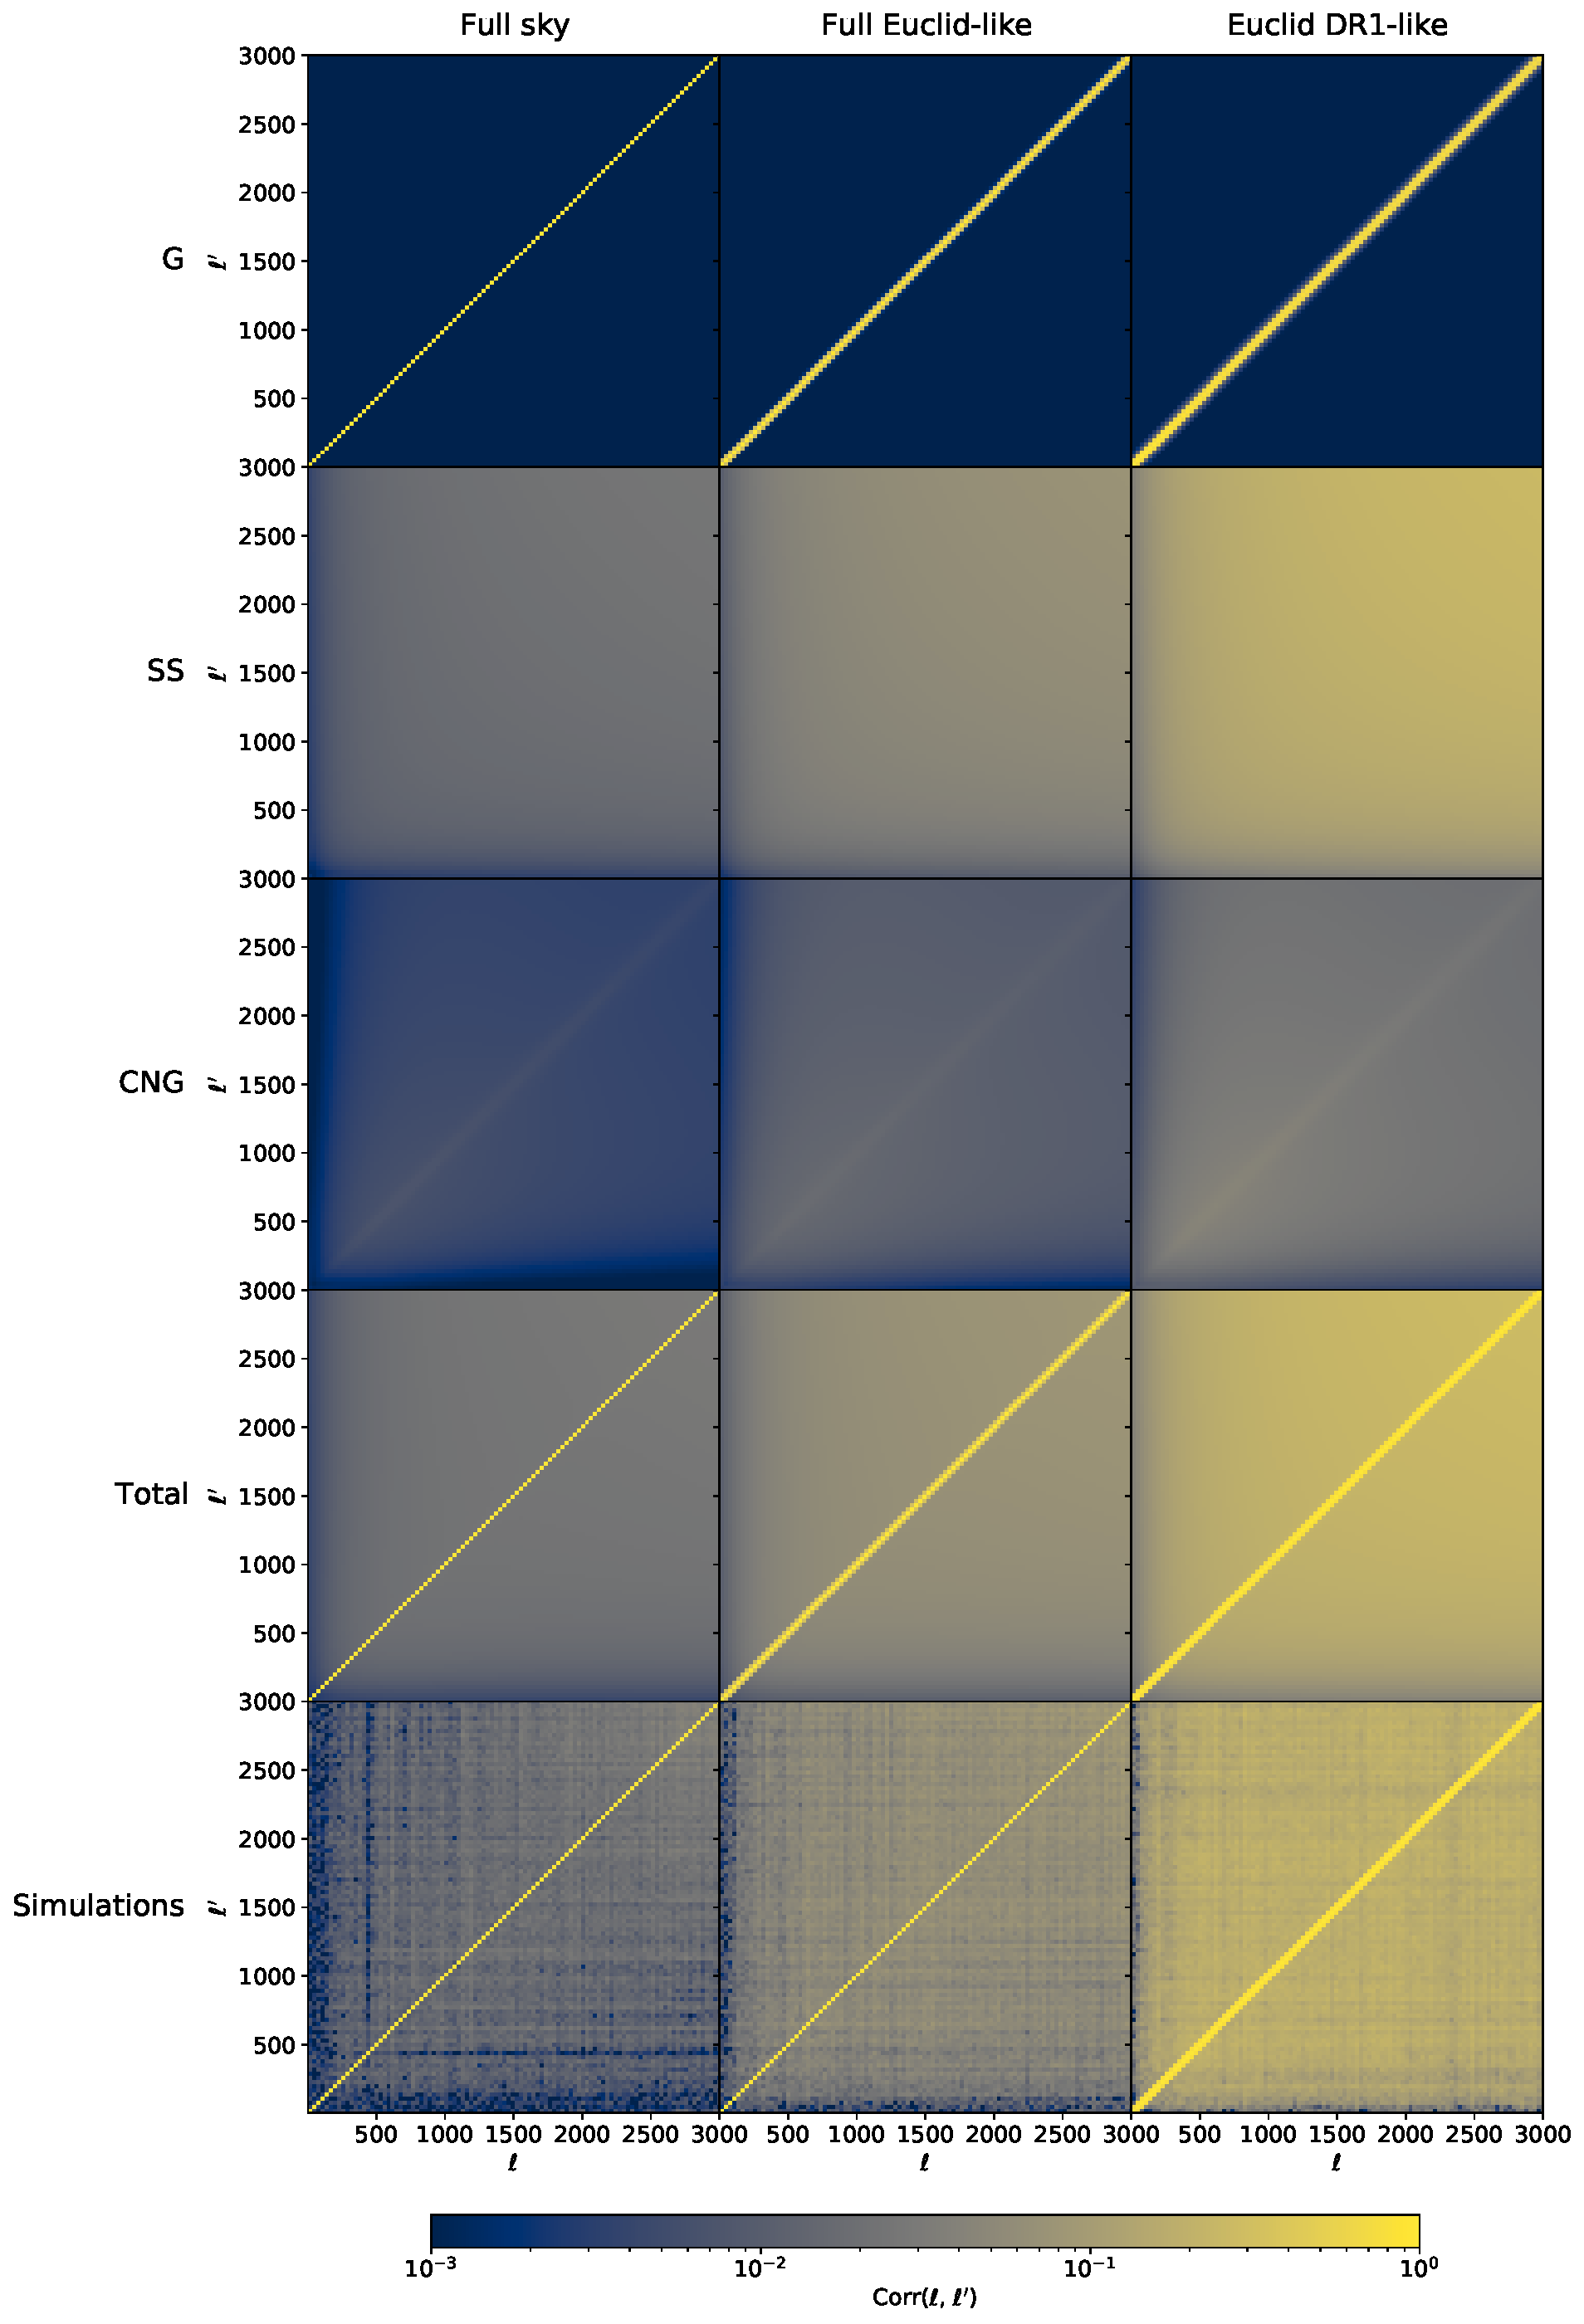
\includegraphics[width=.921\textwidth]{cov_mats} % so not too tall
\caption{Correlation matrices for the simulated covariance compared to the total theoretical covariance for each mask and for the individual components of the theory covariance: Gaussian (G), super-sample (SS), and connected non-Gaussian (CNG). The covariance shown here is for the shear $E$-mode power spectrum in the lowest redshift bin, without shape noise.}
\label{cov_fig:cov_mats}
\end{figure}

\autoref{cov_fig:cov_diags} shows a detailed comparison of certain diagonals of the covariance matrix. For the main diagonal ($\Delta \ell = 0$), the variance divided by the square of the power spectrum is shown, to remove any effects coming from disagreement in the power spectrum between the simulations and theory, which is not the focus of this work. For the off-diagonals ($\Delta \ell =$ 2, 10, 100) the correlation is shown.
In all panels the simulated line is a rolling average over 50 $\ell$s and the shaded region is the standard deviation over this range. For the full-sky and full \Euclid{}-like masks, excellent agreement is observed between the theory and simulations. For the more extreme \Euclid{} DR1-like mask there is a slightly worse, but still generally good, level of agreement. In particular, the super-sample covariance component is clearly correctly increasing with the severity of the sky cut to match the additional correlation found in the simulations. The relative sizes and importance of the three theory contributions are discussed further in \autoref{cov_sec:importance}.
We may conclude from Figures \ref{cov_fig:cov_mats} and \ref{cov_fig:cov_diags} that \texttt{CosmoLike}'s non-Gaussian covariance calculations appear to be suitably accurate, to the degree that can be assessed using these simulations.

\begin{figure}
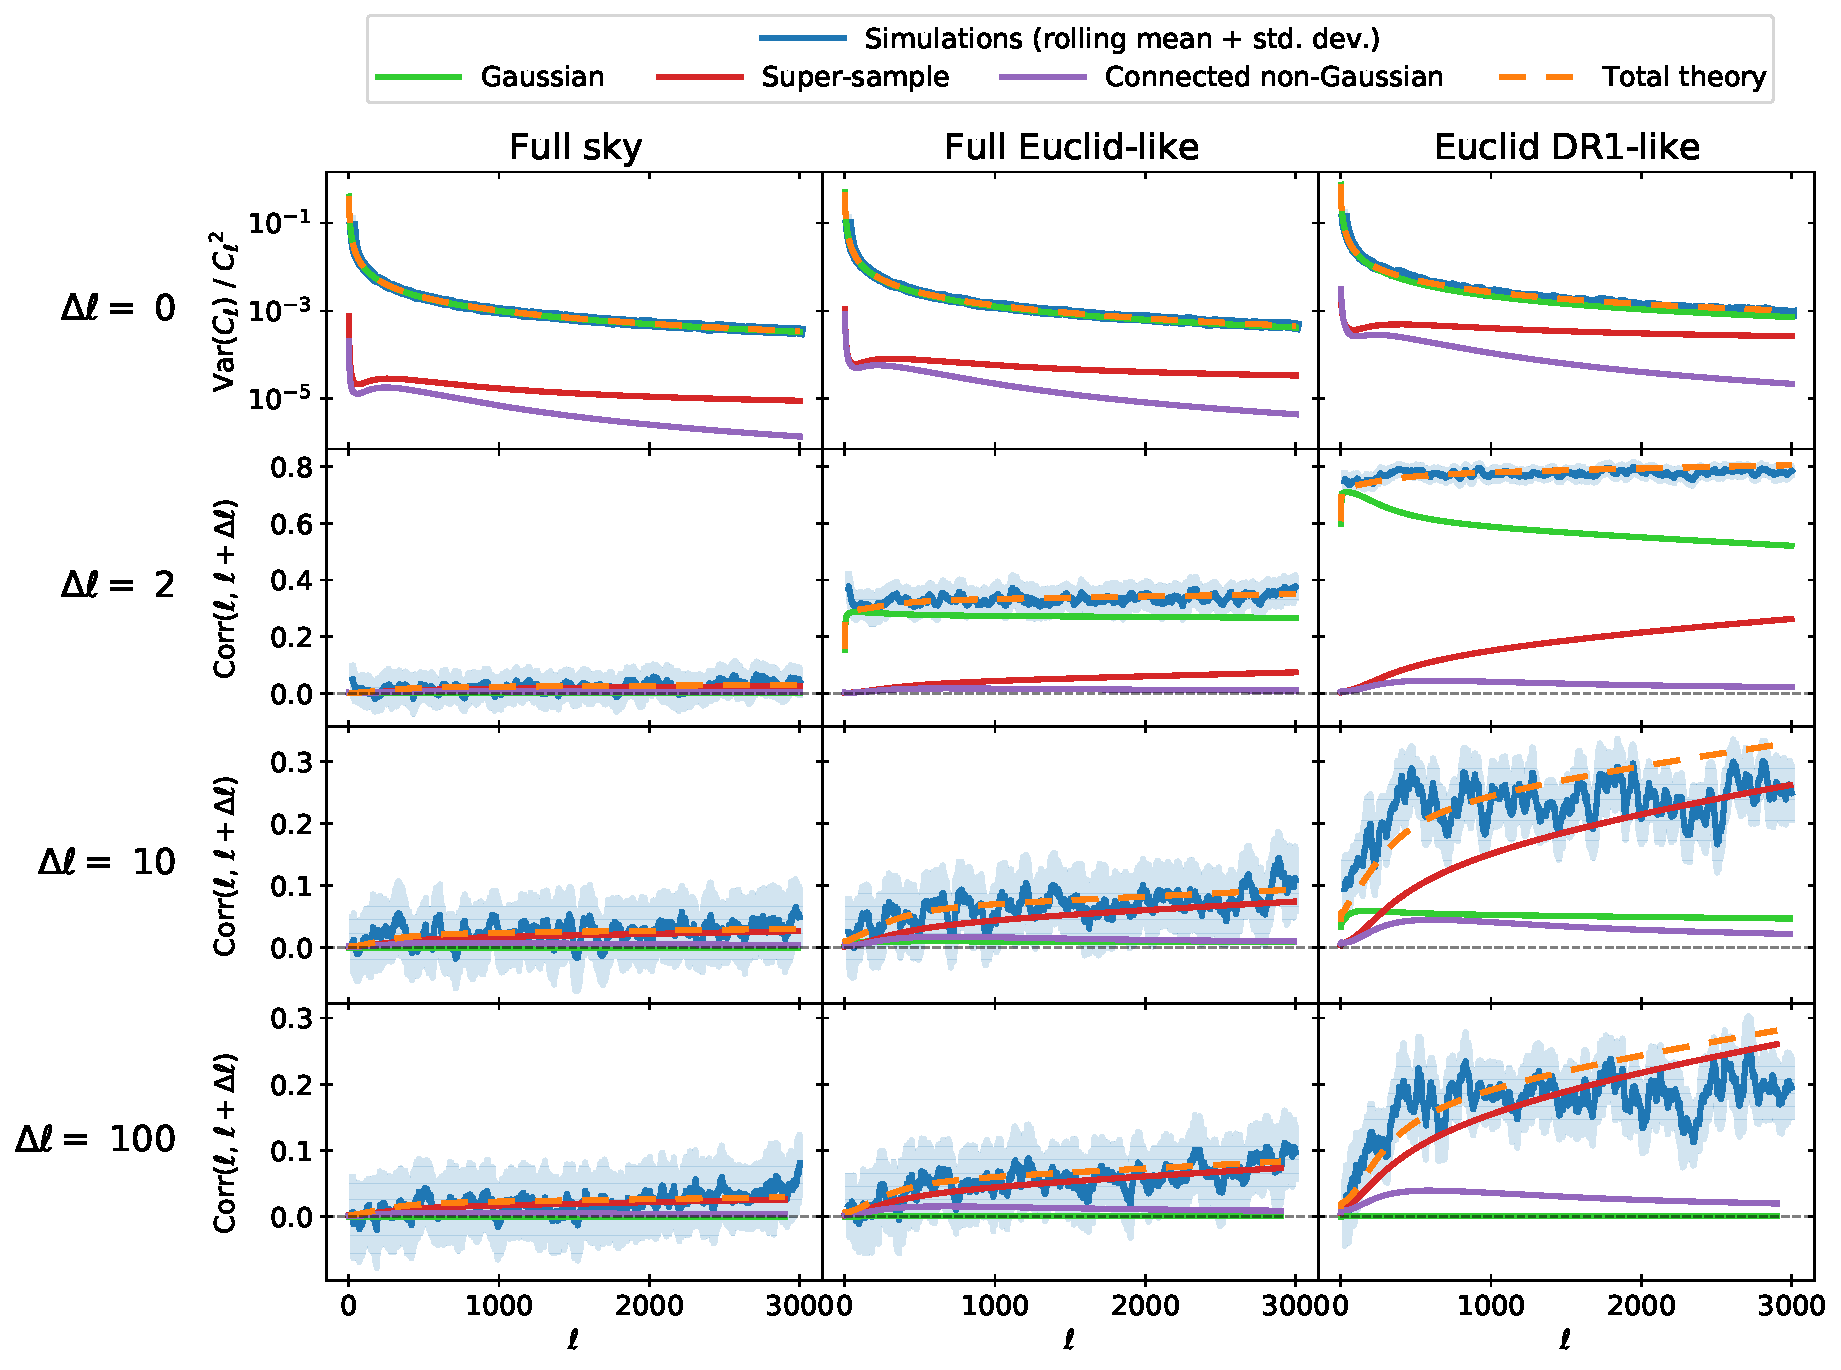
\includegraphics[width=\textwidth]{cov_diags}
\caption{Comparison between the covariance predicted by theory and measured from simulations, for the three masks. The top row shows the variance divided by the power spectrum squared, and the lower three rows show correlation. In all panels the simulated line is a rolling average over 50 $\ell$s, and the shaded region is the standard deviation over this range. The covariance shown here is for the shear $E$-mode power spectrum in the lowest redshift bin, without shape noise.}
\label{cov_fig:cov_diags}
\end{figure}

This comparison was also repeated for purely Gaussian fields, which were simulated using \texttt{healpy}.
The results are shown in \autoref{cov_fig:cov_diags_gauss}, where an excellent level of agreement is observed between the Gaussian field simulations and the prediction from the improved NKA, which is a significant improvement over the standard NKA (not shown).

\begin{figure}
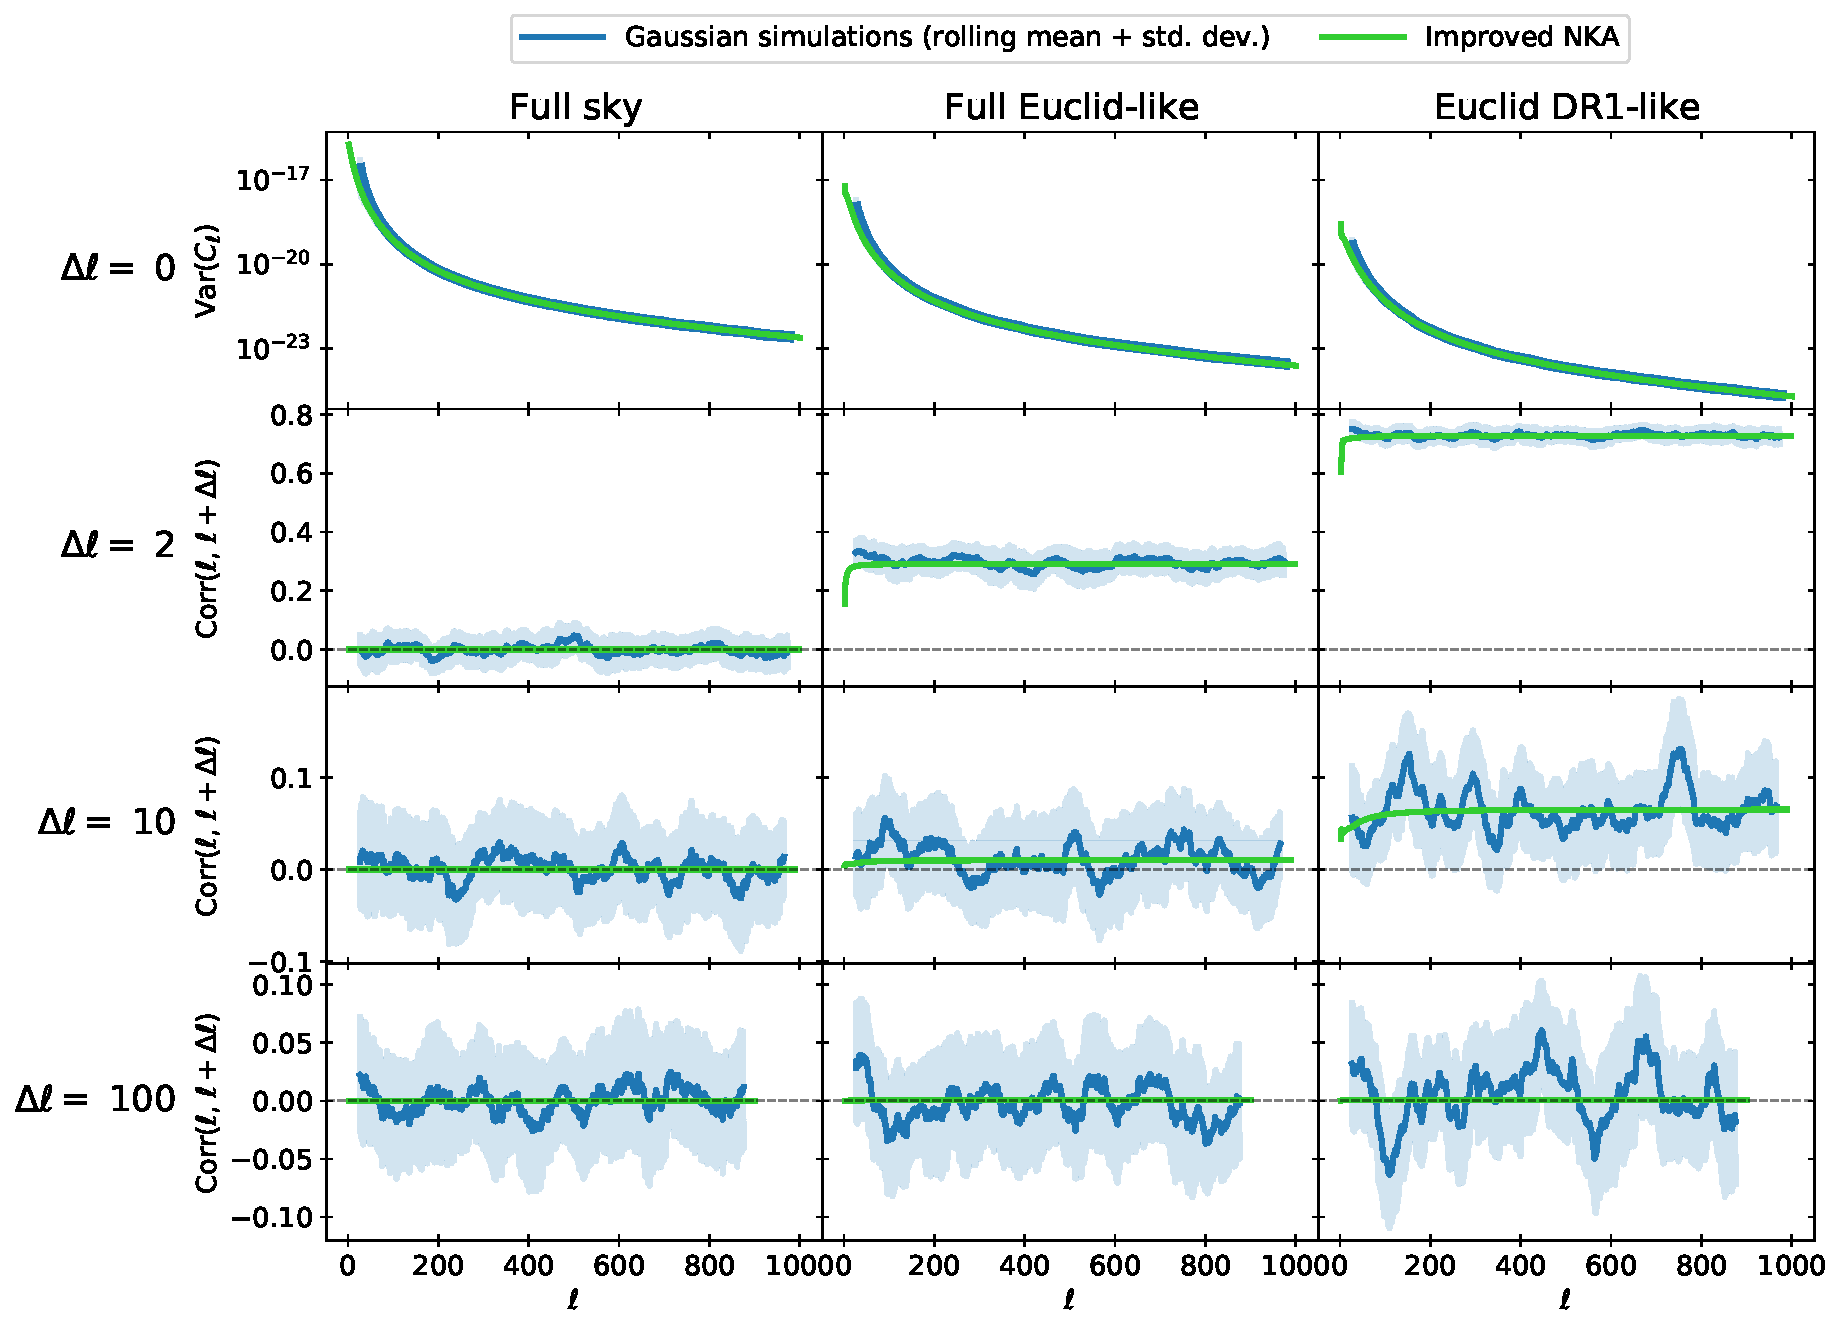
\includegraphics[width=\textwidth]{cov_diags_gauss}
\caption{Comparison between covariance measured from Gaussian field simulations and predicted using the improved NKA method, for the three masks. In all panels the simulated line is a rolling average over 50 $\ell$s, and the shaded region is the standard deviation over this range. No shape noise is included.}
\label{cov_fig:cov_diags_gauss}
\end{figure}

\section{Importance of covariance components and dependence on mask}
\label{cov_sec:importance}

This section addresses the size and importance of the different components of the cosmic shear pseudo-$C_\ell$ covariance, and how these properties depend on the mask.

\subsection{Relative sizes of components}
\label{cov_sec:rel_sizes}

\subsubsection{Without shape noise}

Let us first consider the case without shape noise, which has already been shown in Figures \ref{cov_fig:cov_mats} and \ref{cov_fig:cov_diags}.
It can be seen from the full correlation matrices plotted in \autoref{cov_fig:cov_mats} that the main diagonal of the matrix is dominated by the Gaussian component, which is purely diagonal in the full-sky case and visibly broadens slightly as the sky cut is increased. The super-sample covariance is the dominant off-diagonal component, particularly at higher $\ell$ but extending down visibly even to $\ell < 500$ in the case of the most extreme \Euclid{} DR1-like mask. The connected non-Gaussian contribution is barely visible on the colour scale, other than for the \Euclid{} DR1-like mask at low $\ell$.

A more detailed comparison of the relative sizes of the different components is possible with the selected diagonals shown in \autoref{cov_fig:cov_diags}. Again it is apparent that the main diagonal ($\Delta \ell = 0$) is dominated by the Gaussian component, but the extent to which this is the case is reduced as the sky cut is increased, as the contribution increases from both non-Gaussian components.
Moving away from the main diagonal, at $\Delta \ell = 2$ the Gaussian is still the largest component (except on the full sky, where its contribution is purely diagonal), but by $\Delta \ell = 10$ the super-sample component is dominant and increasing towards higher $\ell$.
It is clear that the super-sample covariance contribution increases with a more severe sky cut, though notably it is still visibly non-zero even for full-sky observations. The connected non-Gaussian component is the subdominant non-Gaussian contribution at all values of $\ell$ and $\Delta \ell$ for all masks.

\subsubsection{With shape noise}

\autoref{cov_fig:cov_diags_withnoise} shows an equivalent comparison of the sizes of the theoretical covariance components with shape noise included.
Gaussian shape noise is assumed, which---as introduced in \autoref{chap:est_like}---is included as a contribution to the power spectrum,
\begin{align}
C_\ell &\rightarrow C_\ell + N_\ell; \\
N_\ell &= \frac{{\sigma_\varepsilon}^2}{N_i},
\label{cov_eqn:nl}
\end{align}
where $\sigma_\varepsilon$ is the intrinsic galaxy shape dispersion per component and $N_i$ is the number of galaxies per steradian per redshift bin. A \Euclid{}-like galaxy number density of $30\,/\,\text{arcmin}^2$, equally split over five redshift bins, was assumed, along with a value of $\sigma_\varepsilon = 0.3$.

\begin{figure}
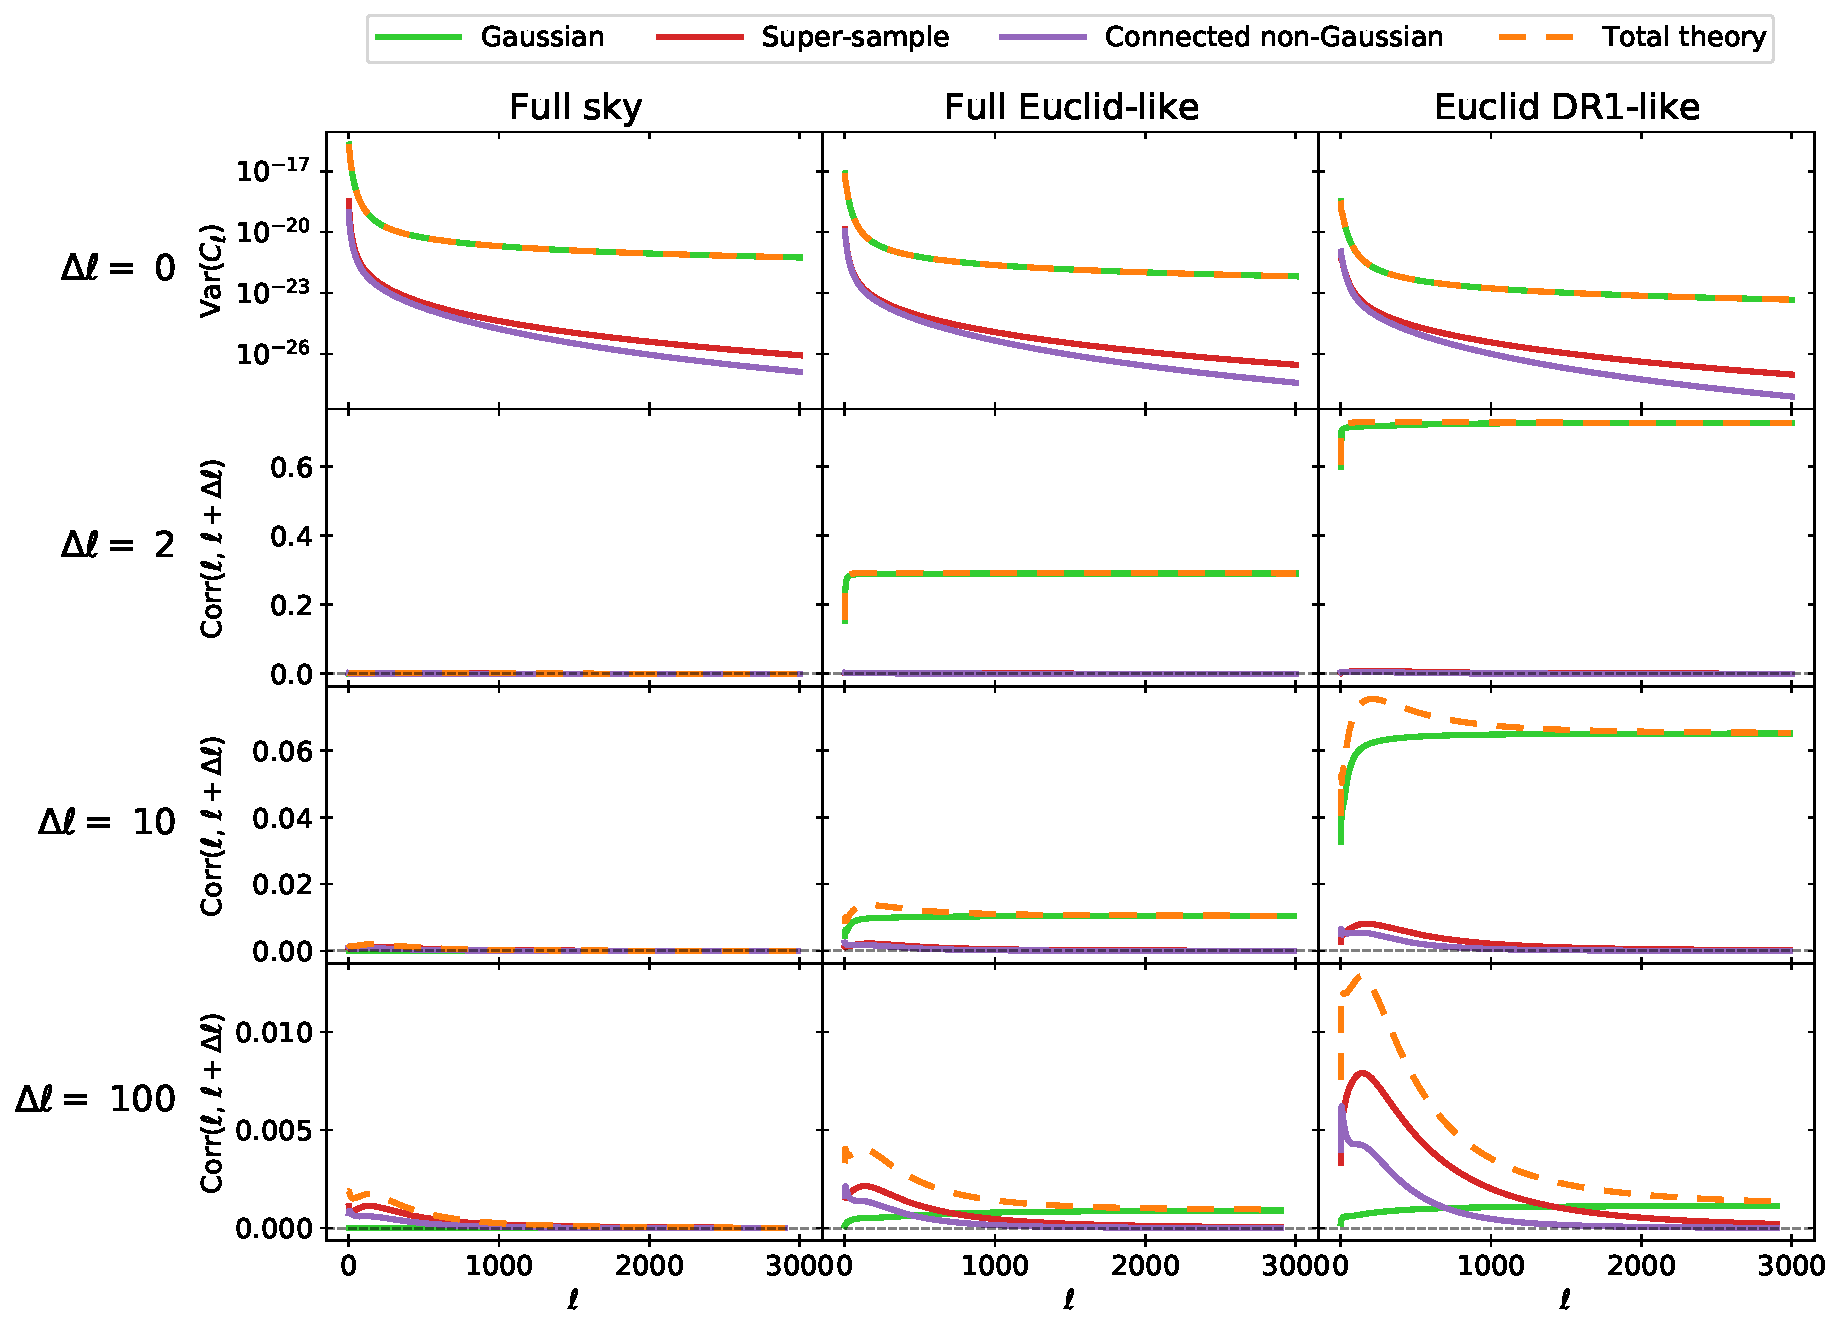
\includegraphics[width=\textwidth]{cov_diags_withnoise}
\caption{Comparison between contributions to the theoretical covariance for the three masks, with shape noise included
following Equation \eqref{cov_eqn:nl}. The top row shows the variance, and the lower three rows show correlation.}
\label{cov_fig:cov_diags_withnoise}
\end{figure}

With shape noise included, quite different behaviour to the no-noise case is found. The Gaussian-dominated main diagonal is substantially increased, especially at higher $\ell$, resulting in non-Gaussian off-diagonal correlations being significantly suppressed.
The result is that the Gaussian component is dominant at all $\ell$ as far away from the main diagonal as $\Delta \ell = 10$.
By $\Delta \ell = 100$, the Gaussian component is no longer dominant at lower $\ell$, but continues to account for the largest contribution at higher $\ell$: above $\ell \sim 1000$ for the full \Euclid{}-like mask and $\ell \sim 1500$ for the \Euclid{} DR1-like mask. This suggests that once shape noise is included, the Gaussian component is more important than the no-noise results in \autoref{cov_fig:cov_diags} suggest.

\subsection{Importance for parameter constraints}
\label{cov_sec:params}

While the relative size of the different covariance components studied in \autoref{cov_sec:rel_sizes} offers interesting insight into their behaviour, it says relatively little about the actual importance of each component. In particular, it is unclear to what extent the dominance of the Gaussian component on and close to the main diagonal is offset by its sub-dominance farther away from the main diagonal.
In this section, to gain more insight into this, mock parameter constraints are produced. Shape noise is included, following Equation \eqref{cov_eqn:nl}.

Here five redshift bins were used, including all auto- and cross-spectra ($E$-modes only), giving 15 power spectra in total.
Scales up to $\ell_\text{max} = 5000$ were included.
The full data vector for this setup would have $n =$ 75\,000 elements ($15 \times 5000$), which gives $n \left( n + 1 \right) / 2 =$ 2.8\,billion unique covariance elements. Due to the time needed to evaluate the projected matter trispectrum, it would be unfeasible to calculate the connected non-Gaussian contribution in full.
As a result, an angular binning approach was taken, with 12 logarithmically spaced bandpowers, and an approximation was used to obtain the connected non-Gaussian bandpower covariance from a more modest number of per-$\ell$ covariance calculations. This approximation is described and validated in \autoref{cov_sec:cng_approx}.
The Gaussian and super-sample covariance components were calculated in full, using scales up to $\ell_\text{max} = 8000$ for intermediate calculations, before being binned into bandpowers as
\begin{equation}
P_b = \sum_\ell \mathbfss{P}_{b \ell} C_\ell,
\label{cov_eqn:cl_to_bp}
\end{equation}
where $\mathbfss{P}$ is the bandpower binning matrix whose elements are given by
\begin{equation}
\mathbfss{P}_{b \ell} =
\begin{cases}
\dfrac{\ell \left( \ell + 1 \right)}{2 \pi}
\left[ \ell_\text{min}^{b + 1} - \ell_\text{min}^b \right]^{-1}
& \text{for } \ell_\text{min}^b \leq \ell < \ell_\text{min}^{b + 1}; \\
0 & \text{otherwise,}
\end{cases}
\label{cov_eqn:pbl}
\end{equation}
where $\ell_\text{min}^b$ is the lower edge of bin $b$.

A mock observation was obtained by sampling from a Gaussian likelihood with the total covariance. The input mean was the fiducial theory power spectra, plus noise for auto-spectra given by Equation \eqref{cov_eqn:nl}, mixed using the mixing matrix obtained using \texttt{NaMaster}, then binned following Equation \eqref{cov_eqn:cl_to_bp}. This random sampling process replicates the randomness of cosmic variance that is present in a real observation, and means that---as with real data---the resulting posterior distributions are not centred on the `true' input parameters.
Checks similar to those shown in \autoref{gl_Sec:nongauss_fields} confirmed that bandpowers measured from the \citet{Takahashi2017} simulations used in \autoref{cov_sec:sims} are no more non-Gaussian than those measured from Gaussian field simulations, and therefore since a Gaussian likelihood was shown to be sufficiently accurate for Gaussian fields in \autoref{chap:gauss_like}, it is a suitable choice here.

Parameter constraints were obtained by iterating over two-parameter grids produced using \texttt{CosmoSIS} \citep{Zuntz2015}, following the pipeline described in \autoref{gl_Sec:fs_method_theory}.\footnote{The pipeline includes the \texttt{CAMB} \citep{Lewis2000, Howlett2012} and \texttt{Halofit--} \texttt{Takahashi} \citep{Smith2003, Takahashi2012} modules.}
All other parameters were held fixed.
At each point in parameter space, theory bandpowers---calculated in the same way as the input mean to the observation described above---were compared to the observed bandpowers using a Gaussian likelihood with different combinations of covariance components.
All combinations necessarily include the Gaussian component, since this on its own is a valid positive definite covariance matrix, unlike the super-sample and connected non-Gaussian components.

\subsubsection{Connected non-Gaussian approximation}
\label{cov_sec:cng_approx}

As noted above, it is impractical to calculate the connected non-Gaussian component for all 2.8 billion unique elements of the full covariance matrix. Instead, an approximation was used to directly obtain its contribution to the bandpower covariance.
This approximation was designed to mimic two effects: the mixing of power by the survey mask, and the binning of individual multipoles into bandpowers. In this analysis, both of these processes are cosmology-independent: each shear field uses the same mask, and all power spectra use the same binning scheme. As a result, both processes should have approximately the same effect on every power spectrum, and consequently also every covariance block. Therefore, the approximation made here uses two sets of weights---one to mimic binning and the other to mimic mixing---which were calibrated for the covariance of the shear auto-power spectrum in the lowest redshift bin and then applied to all further blocks.

First, the connected non-Gaussian component was evaluated in full for a single covariance element per bandpower pair, for all combinations of power spectra. This was chosen to be for the weighted average $\ell$ in each bandpower, with the weights given by $\mathbfss{P}_{b \ell}$ (Equation \ref{cov_eqn:pbl}), rounded to the nearest integer. This vastly reduced the number of projected trispectrum calculations, to 16\,290.\footnote{This number comes from a reduced data vector of 12 bandpowers and 15 power spectra, giving a data vector of length $n = 12 \times 15 = 180$ and a number of unique covariance elements of $n \left( n + 1 \right) / 2 = 16\,290$.}
The result was then re-weighted using the weights calibrated using the covariance of the shear auto-power spectrum in the lowest redshift bin, which was calculated in full for the previous sections.

The weighting can be understood as a two-step process.
First, a `binning' weighting was applied, designed to mimic the effect of taking the full unbinned covariance matrix and binning it into bandpowers. Then a `mixing' weighting was applied, designed to mimic the effect of the mixing matrix. In both cases, the weights were obtained by carrying out the process in full for the shear auto-power spectrum in the lowest redshift bin.

This can be illustrated using equations as follows. For the first block (covariance of shear auto-power in the lowest redshift bin), the following procedure was used to transform the full unbinned covariance $\mathbfss{Cov}_\text{unbinned}$ into a final binned and mixed block $\mathbfss{Cov}_\text{mixed}$, via a binned and unmixed stage $\mathbfss{Cov}_\text{binned}$:
\begin{align}
\mathbfss{Cov}_\text{binned} &=
\mathbfss{P} ~ \mathbfss{Cov}_\text{unbinned} ~
\mathbfss{P}^\intercal; \\
\mathbfss{Cov}_\text{mixed} &=
\mathbfss{M} ~ \mathbfss{Cov}_\text{binned} ~
\mathbfss{M}^\intercal,
\end{align}
where $\mathbfss{P}$ and $\mathbfss{M}$ are the bandpower binning and pseudo-$C_\ell$ mixing matrices, respectively. Elements were selected from $\mathbfss{Cov}_\text{unbinned}$ corresponding to the weighted average $\ell$ within each bandpower to give $\mathbfss{Cov}_\text{sampled}$. The matrices of binning weights $\mathbfss{w}_\text{bin}$ and mixing weights $\mathbfss{w}_\text{mix}$ were then calculated as
\begin{align}
\mathbfss{w}_\text{bin} =
\frac{\mathbfss{Cov}_\text{binned}}
{\mathbfss{Cov}_\text{sampled}}
\qquad&\text{(elementwise);} \\
\mathbfss{w}_\text{mix} =
\frac{\mathbfss{Cov}_\text{mixed}}
{\mathbfss{Cov}_\text{binned}}
\qquad&\text{(elementwise).}
\end{align}
Finally, the sampled covariance blocks $\mathbfss{Cov}_\text{sampled}$ were calculated for every block in the full covariance matrix, and transformed to give approximate binned and mixed covariance blocks as
\begin{alignat}{2}
\mathbfss{Cov}_\text{binned\_approx} &=
\mathbfss{w}_\text{bin} *
\mathbfss{Cov}_\text{sampled}
\qquad&&
\text{(elementwise);} \\
\mathbfss{Cov}_\text{mixed\_approx} &=
\mathbfss{w}_\text{mix} *
\mathbfss{Cov}_\text{binned\_approx}
\qquad&&
\text{(elementwise).}
\end{alignat}
While this two-step weighting process could be equivalently formulated as a single step, separating the effect of the binning and mixing approximations allows for additional insight into their respective effects.

These approximations were validated by carrying out an equivalent process for the super-sample covariance matrix and comparing the results to those obtained using the full correct treatment.
Histograms of the ratios between the approximate and exact covariance for each step, for all elements of the bandpower covariance across all redshift bins, are shown in \autoref{cov_fig:cng_approx}.
Each step introduces a bias of order per cent on average (although conveniently in opposite directions) with a spread of a few per cent.
This is sufficiently accurate for the purposes of this work, especially considering that the connected non-Gaussian component is the smallest of the three, but nevertheless this small potential error should be borne in mind when interpreting the results. Since the super-sample and connected non-Gaussian covariance contributions were shown to be similarly smooth in \autoref{cov_sec:sims}, the fact that this approximation works well for the former suggests that it should too for the latter.

\begin{figure}
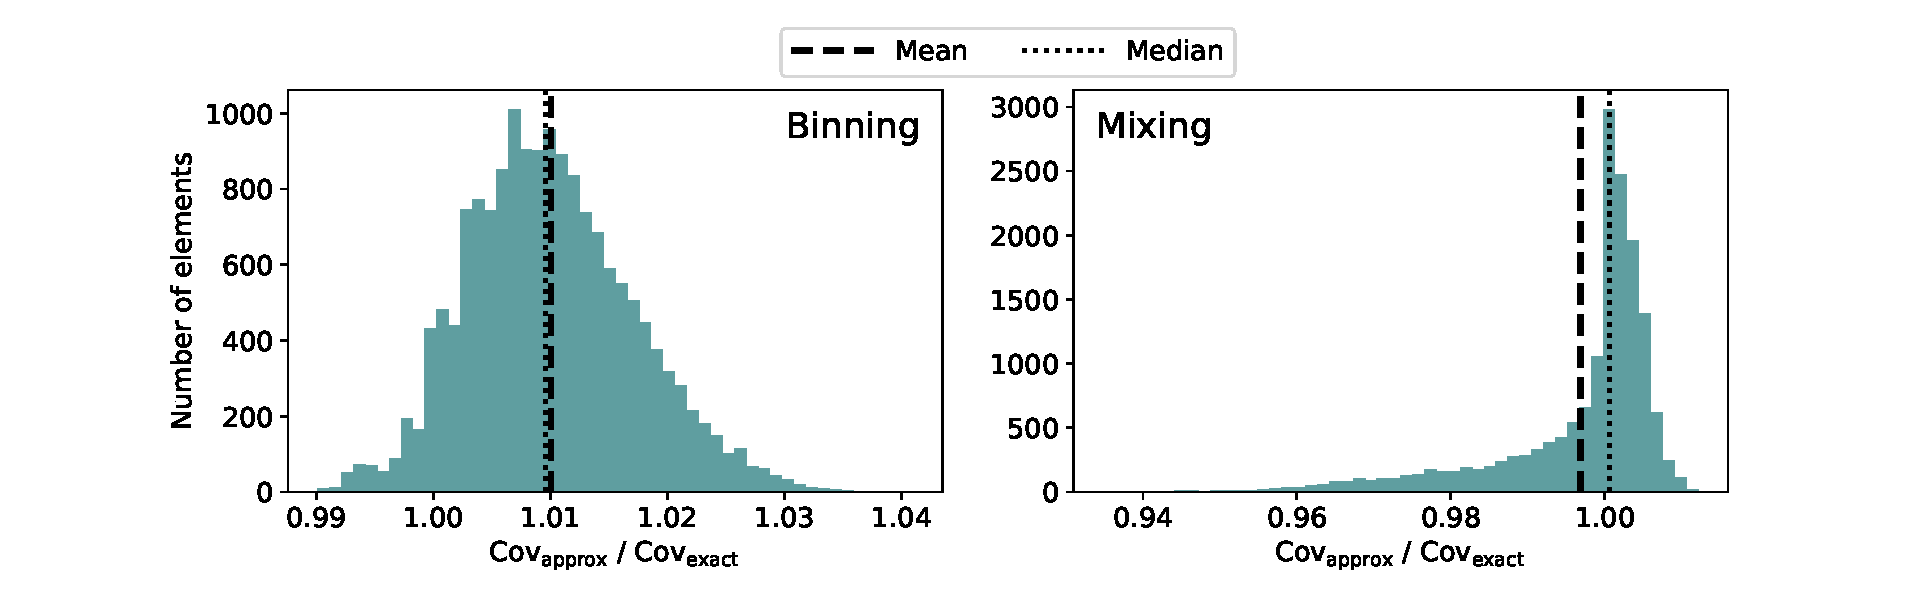
\includegraphics[width=\textwidth]{cng_approx}
\caption{Validation of the connected non-Gaussian approximation used to obtain the mock parameter constraints in \autoref{cov_sec:params}, which is described in \autoref{cov_sec:cng_approx}. Histograms of the ratio of the approximate to exact covariance are shown, for the `binning' (left) and `mixing' (right) steps, for all elements of the bandpower covariance matrix across all redshift bins, measured using the super-sample covariance. The results in all other sections are obtained using the connected non-Gaussian component calculated in full.}
\label{cov_fig:cng_approx}
\end{figure}

\subsubsection{Results}

Two-parameter constraints for different combinations of covariance components are shown in \autoref{cov_fig:2d_constraints}.
The top row shows dark energy equation of state parameters ($w_0$, $w_a$), where $w \left( a \right) = w_0 + w_a \left( 1 - a \right)$.
The bottom row shows the matter density $\Omega_\text{m}$ and the amplitude of the matter power spectrum at $z = 0$ on the scale of $8\,h^{-1}\,\text{Mpc}$, $\sigma_8$.
The three columns are for the three different masks. In each panel, all parameters other than the two shown are held fixed. Only the 1 and 3\,$\sigma$ credible regions are marked, which respectively contain the highest 68.3 and 99.7 per cent of the posterior probability mass. The relative areas of the $3\sigma$ credible region are listed for each combination of parameters and mask in \autoref{cov_tbl:rel_areas}.

\begin{figure}
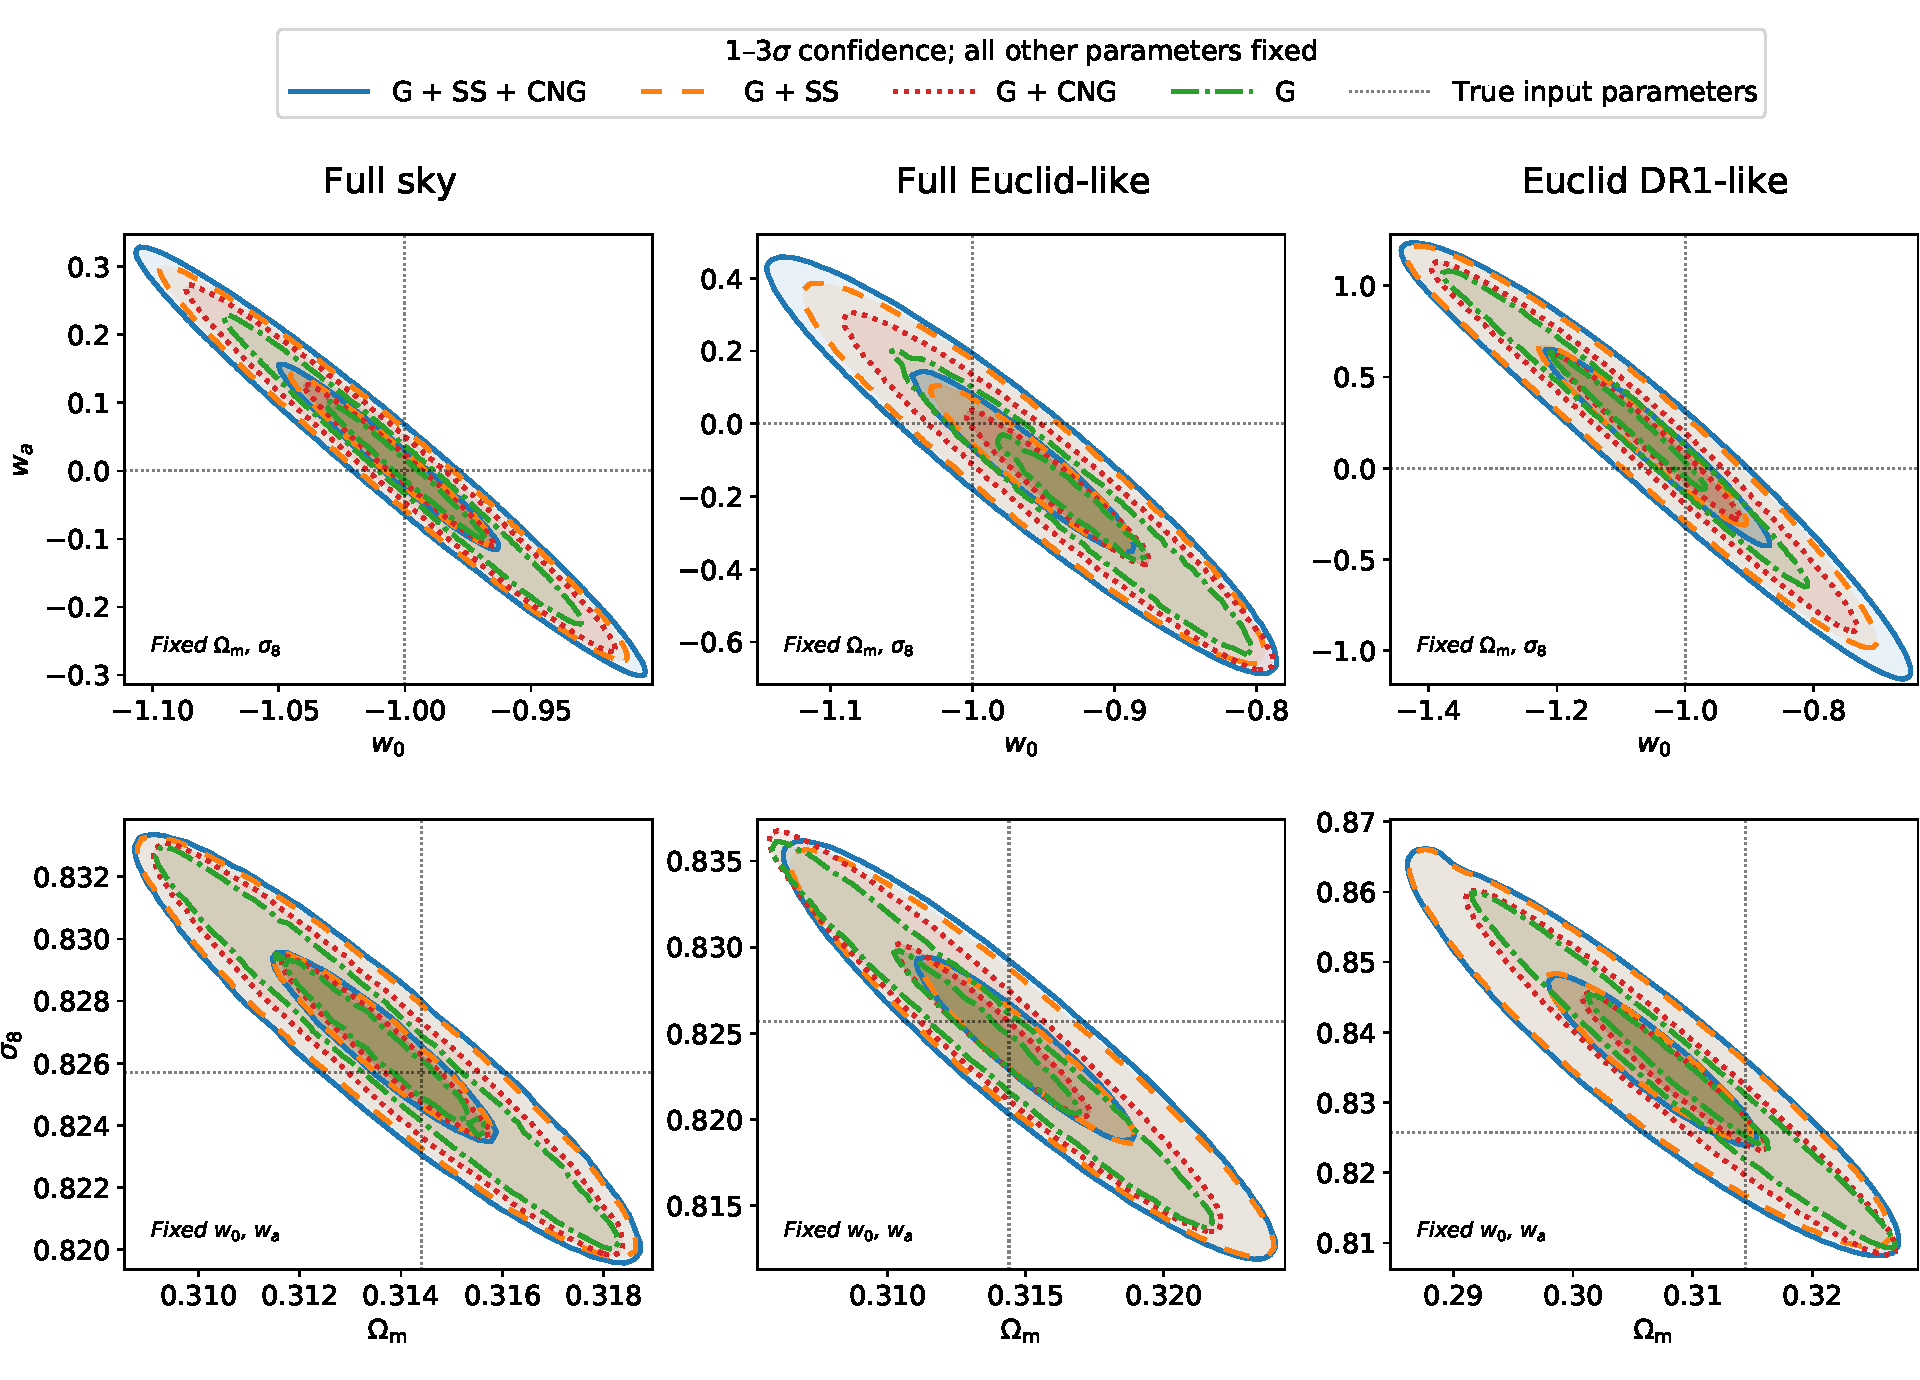
\includegraphics[width=\textwidth]{2d_constraints}
\caption{Two-parameter constraints for different masks and different combinations of covariance contributions: Gaussian (G), super-sample (SS), and connected non-Gaussian (CNG). Shape noise is included, following Equation \eqref{cov_eqn:nl}. In each panel, all parameters other than the two shown are held fixed. Only the 1 and 3\,$\sigma$ credible regions are marked, which respectively contain the highest 68.3 and 99.7 per cent of the posterior probability mass. The relative areas of each $3\sigma$ credible region are listed in \autoref{cov_tbl:rel_areas}. Note that the axis ranges differ between panels.}
\label{cov_fig:2d_constraints}
\end{figure}

\begin{table}[p]
{
\centering
\caption{Relative areas of $3\sigma$ credible regions in \autoref{cov_fig:2d_constraints}.}
\label{cov_tbl:rel_areas}
\vspace{.5em}
\bgroup
\def\arraystretch{1.3}
\begin{tabular}{llrrrr}
\hline
\multirow{2}{*}{Parameters} & \multirow{2}{*}{Mask} & \multicolumn{4}{c}{Relative area of $3\sigma$ credible region (\%)} \\
& & G + SS + CNG & G + SS & G + CNG & G \\ \hline \hline
\multirow{3}{*}{($w_0$, $w_a$)}
& Full sky & 100 & 82 & 63 & 38 \\
& Full \Euclid{}-like mask & 100 & 84 & 61 & 36 \\
& \Euclid{} DR1-like mask & 100 & 85 & 51 & 30 \\ \hline
\multirow{3}{*}{($\Omega_\text{m}$, $\sigma_8$)}
& Full sky & 100 & 90 & 70 & 49 \\
& Full \Euclid{}-like mask & 100 & 90 & 66 & 45 \\
& \Euclid{} DR1-like mask & 100 & 92 & 54 & 37 \\ \hline
\end{tabular}
\egroup

\vspace{1em}

}

{
% \small
% \textbf{Notes.}~
The table shows the relative area of the $3\sigma$ credible region in \autoref{cov_fig:2d_constraints} for each combination of parameters and mask and for different combinations of covariance components: Gaussian (G), super-sample (SS), and connected non-Gaussian (CNG). The relative $1\sigma$ areas are similar to the $3\sigma$ areas.
}
\end{table}

The Gaussian contribution (G) alone only covers 30--38 per cent of the full $3\sigma$ region for ($w_0$, $w_a$) and 37--49 per cent for ($\Omega_\text{m}$, $\sigma_8$). The Gaussian and connected non-Gaussian components combined (G + CNG) cover 51--63 and 54--70 per cent for ($w_0$, $w_a$) and ($\Omega_\text{m}$, $\sigma_8$), respectively, while the Gaussian and super-sample components combined (G + SS) cover 82--84 and 90--92 per cent. These results are broadly in line with the single-parameter error bar ratios obtained in \citet{Barreira2018b}.

There is some amount of apparent mask dependence: as the sky cut is increased, the relative area of G + SS sees a very small increase (by 2--3 per cent) whereas G + CNG and G see larger decreases (by 16--22 and 8--12 per cent, respectively). This is consistent with the expectation that super-sample covariance should become more important as the sky is cut further, since this excludes more modes from the survey.

There are also some small shifts in the posterior means between the different composite covariance results for a given mask, despite the fact that the mean of the Gaussian likelihood used in each case is identical and only the covariance differs. This demonstrates how an incorrect covariance leads to an incorrect weighting of the random scatter present in the data due to cosmic variance, and therefore to posterior constraints having not only the wrong size but an erroneous position too, although this is a small effect.

\subsubsection{Effect of marginalisation over additional parameters}

Motivation to explore the impact of marginalisation over additional parameters on the relative importance of each covariance component is provided by the results of \citet{Barreira2018b}. In that paper, the authors produced mock parameter constraints with different covariance contributions included, both for a single parameter at a time with all others fixed and for five parameters with all five allowed to vary simultaneously. For the latter case, they display marginalised two-parameter constraints \citep[their Figure 3]{Barreira2018b}. For ($w_0$, $w_a$) in particular (and to a lesser extent with some other parameter pairs), the $2\sigma$ credible region obtained with the Gaussian covariance alone appears roughly the same as that for the total covariance, to within the sampling noise. This is in contrast to their single-parameter constraints, for which the Gaussian covariance only produced $\sim$ 50 per cent of the $1\sigma$ uncertainty on $w_0$ obtained using the full covariance (see Figure 2 of \citealt{Barreira2018b}). This raises the question of whether marginalisation might reduce the differences between the constraints obtained using different combinations of covariance components.

Here, this question is investigated by performing a three-parameter likelihood analysis using the full \Euclid{}-like mask over ($w_0$, $w_a$, $\Omega_\text{m}$), with all other parameters still held fixed. One- and two-parameter marginalised constraints are shown in \autoref{cov_fig:3d_constraints}. \autoref{cov_tbl:marg} compares the relative areas and widths of one- and two-parameter $3\sigma$ credible regions before and after marginalisation over a third parameter.

\begin{figure} % [p]
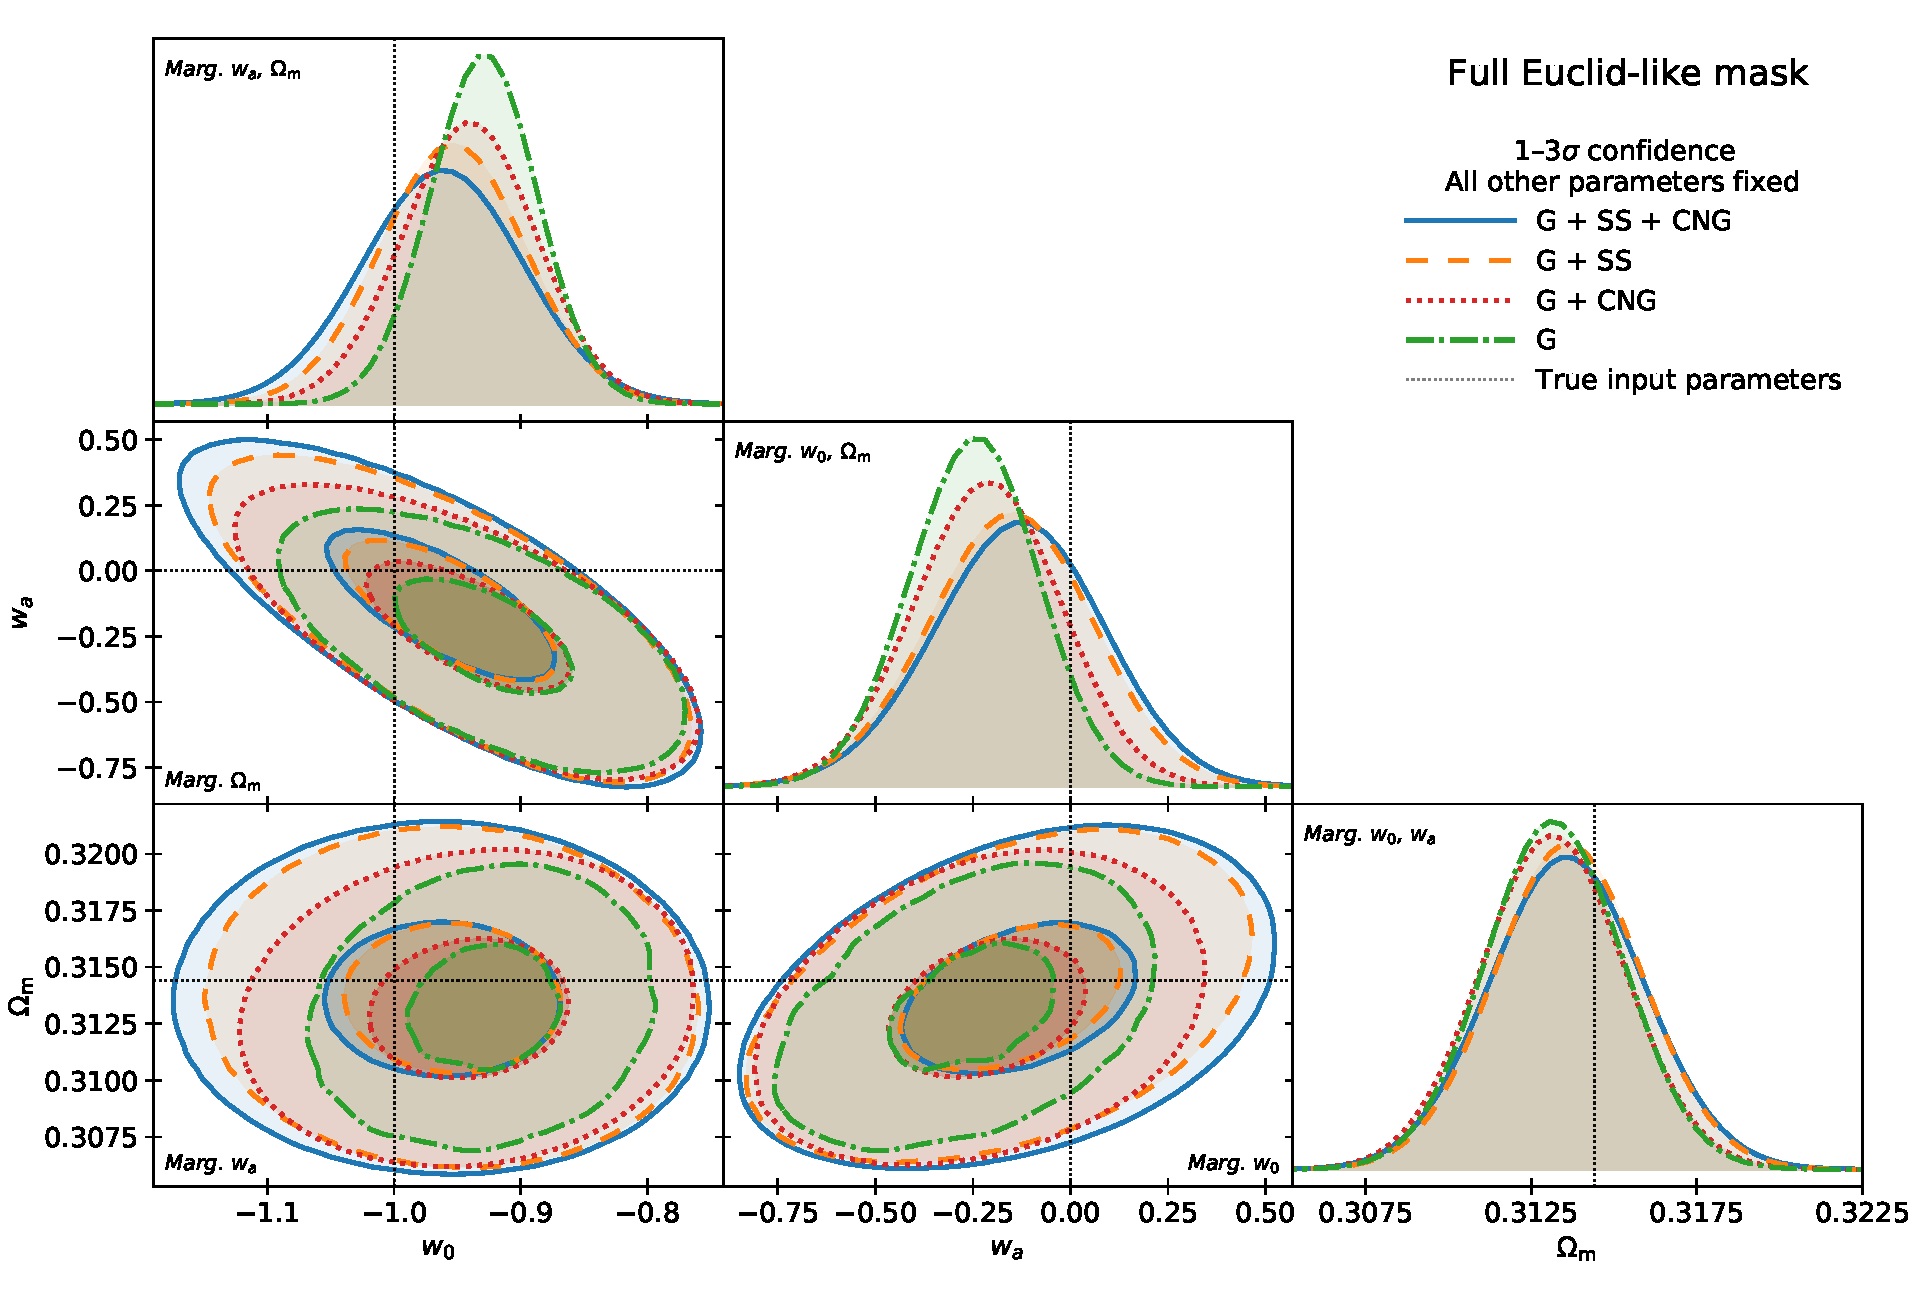
\includegraphics[width=\textwidth]{3d_constraints}
\caption{Two- and one-parameter marginalised constraints obtained from a joint three-parameter analysis of ($w_0$, $w_a$, $\Omega_\text{m}$) for the full \Euclid{}-like mask, including different combinations of covariance contributions: Gaussian (G), super-sample (SS), and connected non-Gaussian (CNG). Shape noise is included, following Equation \eqref{cov_eqn:nl}. The constraints in each panel have been obtained by marginalising over one or two parameters in the joint three-parameter posterior; for example, the panel marked `Marg. $w_a$, $\Omega_\text{m}$' has been marginalised over $w_a$ and $\Omega_\text{m}$. All other parameters are held fixed. Only the 1 and 3\,$\sigma$ credible regions are marked.}
\label{cov_fig:3d_constraints}
\end{figure}

While the relative areas in \autoref{cov_fig:3d_constraints} appear qualitatively similar to those in \autoref{cov_fig:2d_constraints}, there are in fact some substantial quantitative differences, as shown by the values in \autoref{cov_tbl:marg}. In particular, there is almost a doubling in the area of the constraints on ($w_0$, $w_a$) from the Gaussian covariance only (G) relative to the total covariance (G + SS + CNG)---from 36 to 69 per cent---when marginalising over $\Omega_\text{m}$ rather than holding it fixed. A similar but smaller increase is seen for the other subsets (G + SS, G + CNG) of the total covariance for the same parameters.

For constraints on $w_a$ alone, the width of the $3\sigma$ credible region for G relative to G + SS + CNG increases slightly when marginalising over both $w_0$ and $\Omega_\text{m}$ compared to only marginalising over $w_0$, and a similar slight increase is seen for G + SS and G + CNG. However, for constraints on $w_0$, there is a small decrease in relative widths when marginalising over both $w_a$ and $\Omega_\text{m}$ rather than only $w_a$. One reason for this difference in behaviour between $w_0$ and $w_a$ may be that---as seen in \autoref{cov_fig:3d_constraints}---there is clearly a much stronger correlation between $w_a$ and $\Omega_\text{m}$ than between $w_0$ and $\Omega_\text{m}$. Marginalisation over a strongly correlated parameter should broaden constraints more than marginalisation over a more weakly correlated parameter (indeed, marginalisation over a truly independent parameter should have no effect at all), but it is not obvious that this should change the ratio of relative areas rather than simply broadening all constraints by the same factor. Regardless of the origin of this behaviour, it does appear to be the case that marginalisation over additional parameters---particularly those with which the constrained parameters are correlated---affects the relative importance of the difference covariance contributions. This is in agreement with the findings of \citet{Barreira2018b}.

\begin{table}[t]
{
\centering
\caption{Impact of marginalisation on $3\sigma$ credible regions.}
\label{cov_tbl:marg}
\vspace{.5em}
\bgroup
\def\arraystretch{1.3}
\begin{tabular}{llrrrr}
\hline
\multirow{2}{*}{Parameter(s)} & \multirow{2}{*}{Marginalised over} & \multicolumn{4}{c}{Relative area or width of $3 \sigma$ credible region (\%)} \\
& & G + SS + CNG & \quad~ G + SS & \quad~ G + CNG & G \\ \hline\hline
\multirow{2}{*}{($w_0$, $w_a$)}
& --- & 100 & 84 & 61 & 36 \\
& $\Omega_\text{m}$ & 100 & 89 & 84 & 69 \\ \hline
\multirow{2}{*}{$w_0$}
& $w_a$ & 100 & 91 & 88 & 72 \\
& ($w_a$, $\Omega_\text{m}$) & 100 & 90 & 83 & 69 \\ \hline
\multirow{2}{*}{$w_a$}
& $w_0$ & 100 & 88 & 84 & 70 \\
& ($w_0$, $\Omega_\text{m}$) & 100 & 96 & 85 & 74 \\ \hline
\end{tabular}
\egroup

\vspace{1em}

}

{
% \small
The table shows the relative areas (for two-parameter constraints) and widths (for one-parameter constraints) of the $3\sigma$ credible regions obtained using different combinations of covariance contributions, Gaussian (G), super-sample (SS), and connected non-Gaussian (CNG), for the full \Euclid{}-like mask. Each row contains two sub-rows: the top sub-row is based on a two-parameter fit, which is marginalised over zero or one parameters; the bottom sub-row is based on a three-parameter fit, which is marginalised over one or two parameters. The relative $1\sigma$ areas are similar to the $3\sigma$ areas.
}
\end{table}

\section{Conclusions}
\label{cov_sec:conclusions}

As the era of next-generation weak lensing surveys such as \Euclid{} rapidly approaches, it is increasingly important to understand the properties of all steps of an analysis pipeline, including the covariance used in the likelihood.
\autoref{cov_sec:theory} has described how existing publicly available codes can be used in combination to calculate the full covariance matrix of cosmic shear pseudo-$C_\ell$ estimates, including the full details of an arbitrary mask.
It has been further shown in \autoref{cov_sec:sims} that existing simulations can be used to verify the accuracy of a theoretical covariance, which found a high degree of agreement and consistency between theory and simulations. This agreement persists for different masks, showing that the theoretical covariance contributions correctly account for both the cut-sky mode coupling that is inherent to the pseudo-$C_\ell$ method and the non-Gaussian mode coupling, including additional cut-sky super-sample covariance.

This is encouraging for the use of pseudo-$C_\ell$ estimators in weak lensing, whose convenience and speed make them an attractive choice of analysis framework for future surveys. However, an outstanding challenge with such estimators is the need to understand their statistical properties sufficiently well such that they can be used to deliver reliable cosmological constraints to the precision and accuracy needed by future high-precision weak lensing surveys. This challenge has now to a large degree been addressed since it is now known that not only is a Gaussian likelihood sufficient (\autoref{chap:gauss_like}), but a full covariance can be evaluated and validated using the methods shown in this chapter.

The results in this chapter have demonstrated that it is essential to include the non-Gaussian contributions to the covariance, even though cut-sky mode coupling means that the Gaussian covariance component dominates off-diagonal modes close to the main diagonal. The relative size and importance of the Gaussian component increases when including shape noise, but it has been shown in \autoref{cov_sec:importance} that only including the Gaussian component in parameter inference can lead to an underestimation of uncertainties by up to 70 per cent. The dominant non-Gaussian covariance component is the super-sample covariance, but neglecting the subdominant connected non-Gaussian covariance component can still lead to uncertainty underestimation on the scale of 10--20 per cent.
In addition, neglecting some covariance contributions can lead to biases in the position of posterior parameter constraints as well as their size.
However, a real cosmological analysis will require marginalisation over many nuisance parameters, which will decrease the relative importance of all cosmological contributions to the covariance, so these values should be taken as upper limits on the importance of each component.
Perhaps for this reason it was found in the analysis of DES Year 3 data in \citet{Friedrich2021} that the connected non-Gaussian contribution could be entirely neglected, but the results of this work suggest that this conclusion cannot be automatically extended to a \Euclid{}-like survey.
However, this need not be an inconvenience, since approximations of the kind described in \autoref{cov_sec:cng_approx} can be used to obtain the connected non-Gaussian component in a manageable amount of time with a loss of accuracy of only a few per cent on an already subdominant term. Finally, this chapter has shown that marginalisation over additional cosmological parameters may have a substantial effect on the relative importance of the different covariance components. We may conclude from this that it is important to take all marginalisation into account when, for example, determining the required accuracy of theoretical results for a particular science goal or producing forecasts of parameter constraints.
The consistency of these results with those of \citet{Barreira2018b} implies that cut-sky mode coupling has relatively little impact on the respective importance of the covariance components.

% % Uncomment to build alone without subfiles:
% \printbibliography[heading=bibintoc]
% \end{document}


% Binning dependence

% % Uncomment to build this alone without subfiles:
% % (also stuff at bottom)
% % \documentclass[draft]{scrbook} % visualise overfull hbox
% \documentclass{scrbook}
% % Koma script document options
\KOMAoption{paper}{a4}
\KOMAoption{fontsize}{11pt}
\KOMAoption{parskip}{half-} % paragraph spacing
% \KOMAoption{numbers}{enddot} % dot after section number
\KOMAoption{cleardoublepage}{plain} % include page numbers on blank pages
\KOMAoption{chapterprefix}{true} % 'Chapter' before number

% Packages
\usepackage{amsmath} % Gives \text command inside maths blocks
\usepackage{amssymb} % Various maths symbols
\usepackage{array} % Table formatting
\usepackage{bm} % Bold maths including Greek
\usepackage[format=plain]{caption} % Font sizing and alignment in captions
\usepackage{enumitem} % Allows numbering like 1.1 in ordered lists
% \usepackage{float} % Allows H placement of floats
\usepackage{graphicx}
\usepackage[hidelinks]{hyperref} % Hyperlinks without looking like it
% \usepackage{longtable} % Multi-page tables
% \usepackage{multicol} % For columns in text (not tables)
\usepackage{multirow} % For tables
\usepackage{neuralnetwork} % Neural net diagram
\usepackage{pdflscape} % Gives landscape environment
% \usepackage{scrlayer-scrpage} % To move page numbers
\usepackage{tabularx}
\usepackage{textcomp} % Added to fix \textasciiacute error on laptop
% \usepackage{tikz} % Diagrams (used for neural network example)
% \usepackage[pagenumberwidth=3em]{tocbasic}
% \usepackage{tocstyle} % ToC styling
\usepackage{upgreek} % Non-italic greek letters
\usepackage{xpatch} % Biblatex customisation

\usepackage[a4paper, inner=40mm, outer=15mm, top=30mm, bottom=30mm,footskip=15mm, headsep=15mm]{geometry}
% \usepackage[a4paper, inner=40mm, outer=30mm, top=50mm, bottom=50mm,footskip=20mm, headsep=20mm]{geometry} % footskip is space between footer (i.e. page number) and bottom of text
% min allowed is inner 40 mm, others 15 mm

\pagestyle{plain} % no header for front matter, overridden at end of front matter

% Caption setup
% \tablecaptionabove
\captionsetup[table]{labelsep=space}
% \captionsetup[table]{labelsep=space, skip=50pt, position=top}
\captionsetup[figure]{labelsep=space} % labelsep prevents dot followed by colon in captions

% Line spacing
\usepackage{setspace}
% \setstretch{1.4} % strangely this is > \onehalfspacing but < \doublespacing
\onehalfspacing
% \doublespacing

\raggedbottom % prevent huge spaces between paragraphs

% % % % % % % % % % % % % % % % % % % % % % % % %
% Font setup
% \usepackage{mathpazo} % Covers maths mode too
\usepackage[sc]{mathpazo} % Covers maths mode too, sc enables small caps
% \usepackage{palatino}
\usepackage[T1]{fontenc} % 8-bit font encoding
\addtokomafont{disposition}{\rmfamily} % Use serif throughout
% % % % % % % % % % % % % % % % % % % % % % % % %

% % % % % % % % % % % % % % % % % % % % % % % % %
% Section formatting setup
% \RedeclareSectionCommand[beforeskip=0pt]{chapter}
\RedeclareSectionCommand[beforeskip=0pt, innerskip=0pt]{chapter}
\RedeclareSectionCommand[beforeskip=10pt]{subsubsection}
\RedeclareSectionCommand[afterskip=1pt]{subsubsection}
% \setcounter{secnumdepth}{\subsubsectionnumdepth} % number up to subsubsections

% No dot after chapter number (https://tex.stackexchange.com/a/484727)
\renewcommand*{\chapterformat}{%
  \mbox{\chapappifchapterprefix{\nobreakspace}\thechapter
  \IfUsePrefixLine{}{\enskip}}%
}

% In the running header, separate chapter number and name with em dash
\renewcommand*{\chaptermarkformat}{%
\chapapp~\thechapter~---~}

% Create subsubsubsection below subsubsection but above paragraph, following https://tex.stackexchange.com/a/356574

\DeclareNewSectionCommand[
  style=section,
  counterwithin=subsubsection,
  afterskip=1pt,
  beforeskip=10pt,
  % afterskip=1.5ex plus .2ex,
  % beforeskip=3.25ex plus 1ex minus .2ex,
  % afterindent=false,
  level=\paragraphnumdepth,
  tocindent=10em,
  tocnumwidth=5em
]{subsubsubsection}
\setcounter{secnumdepth}{\subsubsubsectionnumdepth}
% \setcounter{tocdepth}{\subparagraphtocdepth}
\setcounter{tocdepth}{\subsubsubsectionnumdepth}

\RedeclareSectionCommands[
  level=\numexpr\subsubsubsectionnumdepth+1\relax,
  toclevel=\numexpr\subsubsubsectiontocdepth+1\relax,
  increaselevel,
]{paragraph,subparagraph}
\RedeclareSectionCommand[
  counterwithin=subsubsubsection,
  tocindent=12em,
  tocnumwidth=6em,
  beforeskip=10pt,
  afterskip=1pt, % line break after paragraph title
]{paragraph}
\RedeclareSectionCommand[
  tocindent=14em,
  tocnumwidth=7em,
  beforeskip=0pt
]{subparagraph}
% % % % % % % % % % % % % % % % % % % % % % % % %

% Autoref capitalisation
\def\chapterautorefname{Chapter}
\def\sectionautorefname{Section}
\def\subsectionautorefname{Section}
\def\subsubsectionautorefname{Section}

% % % % % % % % % % % % % % % % % % % % % % % % %
% Bibliography setup
\usepackage[backend=biber,
    % style=authoryear,
    style=authoryear-comp, % Don't repeat same author(s) in multiple citations
    giveninits=true,
    useprefix=true, % 'van der' etc.
    url=false,
    doi=false,
    isbn=false,
    eprint=false,
    uniquename=false, % Don't add initials in citation to disambiguate between authors with the same surname
    uniquelist=false, % Don't disambiguate in citation between different 'et al.' teams
    maxbibnames=10,
    minbibnames=10,
    maxcitenames=3,%  # 2,
    natbib, % Gives citep and citet commands
    labelalpha=true, % Use an 'alpha' label for each bib entry
    maxalphanames=1, % Use first author as the alpha label
    sorting=anyvt, % Sort by alpha (first author) then year
    block=par, % New line between 'blocks' of the bib entry
    dashed=false, % Reprint author list for each publication in bibliography
    sortcites=false % Show citations in the order supplied
]{biblatex}

% Citation/reference parameters
\renewcommand*{\nameyeardelim}{\addspace} % Space between author and year rather than comma
\renewcommand*{\finalnamedelim}{\addspace\&\addspace} % Ampersand rather than 'and'
\xpatchbibmacro{name:andothers}{{\finalandcomma}}{\addspace}{}{} % Space before 'et al.' rather than comma

% Citation-specific parameters
\DeclareCiteCommand{\blindcite}{\unspace}{}{}{\mancite} % Easy manual citations

% Reference-specific parameters
\AtEveryBibitem{\clearfield{title}} % Suppress title
\AtEveryBibitem{\clearfield{month}} % Suppress month
\DeclareNameAlias{author}{family-given} % Surname first for not just the first author
\DeclareNameAlias{editor}{family-given} % Same for editors
\renewbibmacro{in:}{} % Remove 'In:'
\DeclareFieldFormat{journaltitle}{#1} % Journal title in normal font rather than italics
\renewbibmacro*{volume+number+eid}{\printfield{volume}\printfield{number}\setunit{\addcomma\space}\printfield{eid}} % No dot after issue
\DeclareFieldFormat[article]{number}{\mkbibparens{#1}} % Volume in brackets
\DefineBibliographyStrings{english}{page = {}, pages = {}} % Suppress 'p.'/'pp.'
\renewbibmacro*{date+extradate}{\printtext{\printfield{year}\addcomma}} % Year not in brackets
\DeclareFieldFormat{pages}{\mkfirstpage[{\mkpageprefix[bookpagination]}]{#1}} % Only give starting page
\DeclareFieldFormat{url}{\url{#1}} % No 'URL' before URLs
% \renewcommand{\finentrypunct}{} % Remove final full stop
\renewcommand*{\newunitpunct}{\addcomma\space} % Commas between elements of bibitems

\DeclareBibliographyDriver{book}{%
  \printnames{author}%
  \space
  \printfield{year}%
  \newunit\newblock
  \printfield{booktitle}%
  \newunit
  , \printlist{publisher}%
\finentry}

\DeclareBibliographyDriver{inproceedings}{%
  \printnames{author}%
  \space
  \printfield{year}%
  \newunit\newblock
  \printfield{booktitle}%
  \newunit
  \printfield{volume}%
  \newunit
  \printfield{pages}%
\finentry}

\DeclareBibliographyDriver{incollection}{%
  \printnames{author}%
  \space
  \printfield{year}%
  \newunit\newblock
  \printfield{booktitle}%
  \newunit
  , ed. \printnames{editor},%
  \newunit\newblock
  \printlist{publisher}%
\finentry}

\DeclareBibliographyDriver{misc}{%
  \printnames{author}%
  \space
  \printfield{year}%
  \newunit\newblock
  \printfield{title}%
  \newunit
  \printfield{url}%
\finentry}

\addbibresource{refs.bib}
% % % % % % % % % % % % % % % % % % % % % % % % %

% Footnote spacing
% \deffootnote[1em]{1.5em}{1em}{\textsuperscript{\thefootnotemark~}}
\deffootnote[1em]{1em}{1em}{\textsuperscript{\thefootnotemark~}}

% Testing setting all penalties to zero
\binoppenalty=0
\brokenpenalty=0
\clubpenalty=0
\displaywidowpenalty=0
\exhyphenpenalty=0
\floatingpenalty=0
\hyphenpenalty=0
\interlinepenalty=0
% \linepenalty=0 % allowing this to be zero splits titles in a strange way
\postdisplaypenalty=0
\predisplaypenalty=0
\relpenalty=0
\widowpenalty=0

% Shorthands (non-Maths)
\newcommand{\lcdm}{$\Lambda$CDM}
\newcommand{\wcdm}{$w$CDM}
\newcommand{\Euclid}{\textit{Euclid}}
\newcommand{\Planck}{\textit{Planck}}
\newcommand{\Pcl}{Pseudo-$C_\ell$}
\newcommand{\pcl}{pseudo-$C_\ell$}
\newcommand{\ttp}{3$\times$2\,pt}

% Maths shorthands
\newcommand{\alm}{a_{\ell m}}
\newcommand{\Cl}{C_\ell}
\newcommand{\fsky}{f_\text{sky}}
\newcommand{\lmax}{\ell_\text{max}}
\newcommand{\lmin}{\ell_\text{min}}
\newcommand{\leff}{\ell_\text{eff}}
\newcommand{\tmin}{\theta_\text{min}}
\newcommand{\mathbfit}[1]{\bm{\mathit{#1}}}
\newcommand{\mathbfss}[1]{\bm{\mathsf{#1}}} % to match MNRAS \mathbfss
\renewcommand{\Re}{\operatorname{Re}}
\renewcommand{\Im}{\operatorname{Im}}

% ΛCDM parameters (maths mode)
\newcommand{\wo}{w_0}
\newcommand{\wa}{w_a}
\newcommand{\omm}{\Omega_\text{m}}
\newcommand{\omb}{\Omega_\text{b}}
\newcommand{\omc}{\Omega_\text{c}}
\newcommand{\sie}{\sigma_8}

% % Editing only
% \usepackage{xcolor}
% \newcommand{\todo}[1]{\textbf{{\color{red}{#1}}}}


% \usepackage{subfiles} % Best to do this last apparently

% \pagestyle{headings}
% \setcounter{chapter}{5} % deliberately 1 too low
% \begin{document}

% Uncomment to use subfiles:
% \documentclass[../Thesis.tex]{subfiles}
% \begin{document}

\chapter{Dependence of cosmological parameter constraints on angular binning of weak lensing two-point statistics}
\chaptermark{Dependence of parameter constraints on angular binning of two-point statistics} % short title for running header
\label{chap:binning}
\graphicspath{{../Figs/binning/}{Figs/binning/}}

\section{Introduction}

As introduced in \autoref{chap:est_like}, two-point statistics of weak lensing shear and galaxy number overdensity may be calculated in spherical harmonic space to estimate power spectra, or in real (also called configuration) space to estimate correlation functions. In either case, it is usually necessary to apply an angular binning in $\ell$ or $\theta$. For the power spectrum, this is not strictly necessary in principle, provided the effect of the survey mask is forward modelled rather than removed with a mixing matrix inversion (see the discussion of the \pcl{} method in \autoref{est_Sec:pcl}). However, a realistic \ttp{} analysis setup with 10 tomographic redshift bins and a scale cut of $\lmax = 5000$ would have a data vector with over a million elements if no angular binning was applied, which would be highly impractical. Furthermore, the smooth nature of weak lensing power spectra means that retaining a perfect angular resolution is probably unnecessary. For the correlation function, on the other hand, it is intrinsically necessary to bin in $\theta$, since galaxy pair separation is a continuous quantity sampled at particular points determined by the set of galaxies in the survey.

Varying numbers of angular bins have been used in recent weak lensing analyses. The Dark Energy Survey Year 3 analysis in \citet{DES2021} used 20 correlation function bins from 2.5 to 250 arcmin, while the KiDS-1000 analysis used 9 bins from 0.5 to 300 arcmin, and 8 bandpowers from $\ell = $ 100 to 1500 \citep{Joachimi2021, Heymans2021, Asgari2021}. The Hyper Suprime-Cam Year 1 \pcl{} analysis in \citet{Hikage2019} used 15 bandpowers from $\ell =$ 60 to 6500, though only 6 from $\ell =$ 300 to 1900 were retained in the cosmological analysis.

This chapter explores how many angular bins are necessary to retain a sufficient amount of constraining power in cosmological parameters. Specifically, it studies how the relative size of posterior uncertainties depends on the number of angular bins, both for the power spectrum and correlation function. Since angular binning will be essential in practice for upcoming Stage IV weak lensing surveys, it is vital to understand the relationship between this binning and cosmological parameter constraints in order to strike the optimal balance between computational viability and scientific value.

The main analysis of this chapter is contained within \autoref{bin_sec:main_analysis}, which studies how the size of parameter posterior uncertainties depends on the number of angular bins. In \autoref{bin_sec:additional_effects} a number of additional effects that may affect these results are examined. Conclusions are discussed in \autoref{bin_sec:conclusions}.

\section{Dependence of posterior uncertainties on number of angular bins}
\label{bin_sec:main_analysis}

This section contains the main analysis of the chapter. The method of measuring posterior uncertainties is described in \autoref{bin_sec:method}, while the observed dependence on the number of angular bins is described in \autoref{bin_sec:results}.

\subsection{Measurement of posterior uncertainties}
\label{bin_sec:method}

The posterior uncertainties in this section are measured directly from posterior distributions resulting from a full likelihood analysis. Later in the chapter, in \autoref{bin_sec:additional_effects}, methods will be described and used which approximate these results without the need for a full likelihood analysis.

The different elements of the likelihood analysis will now each be described.

\subsubsection{Modelling of two-point statistics}
\label{bin_sec:modelling}

\ttp{} power spectra were generated using \texttt{CosmoSIS} \citep{Zuntz2015}, covering a two-dimensional grid of values of $w_0$ and $w_a$, and one-dimensional grids of five other cosmological parameters ($\Omega_\text{m}$, $\Omega_\text{b}$, $\sigma_8$, $n_\text{s}$, $h$), with all other parameters held at fixed values in each case.
The pipeline is the same as described in \autoref{gl_Sec:fs_method_theory}, with five Gaussian redshift bins centred on $z =$ 0.65, 0.95, 1.25, 1.55, 1.85. Multipoles up to $\lmax = 5000$ were generated, but different scale cuts are explored in this chapter.
Power spectra were binned into bandpowers following Equation \eqref{cov_eqn:pbl}.

Angular-bin-averaged correlation functions for galaxy position $\xi_{NN}$, shear $\xi_\pm$, and their cross correlation $\xi_{NE}$, were calculated directly from the unbinned power spectra using the following relations:
\begin{align}
\xi_{NN} \left( \theta, \Delta \theta \right) &= \sum_\ell
\frac{2 \ell + 1}{4 \pi} C_\ell \,
\overline{d^\ell_{00}} \left( \theta, \Delta \theta \right);
% \end{equation}
% \begin{equation}
\\
\xi_\pm \left( \theta, \Delta \theta \right) &= \sum_\ell
\frac{2 \ell + 1}{4 \pi} C_\ell \,
\overline{d^\ell_{\pm22}} \left( \theta, \Delta \theta \right);
% \end{equation}
% \begin{equation}
\\
\xi_{NE} \left( \theta, \Delta \theta \right) &= \sum_\ell
\frac{2 \ell + 1}{4 \pi} C_\ell \,
\overline{d^\ell_{20}} \left( \theta, \Delta \theta \right),
\end{align}
where $\overline{d^\ell_{m' m}} \left( \theta, \Delta \theta \right)$ is the bin-averaged Wigner small-$d$ symbol. Following \citet{Fang2020b} and \citet{Stebbins1996}, the small-$d$ symbols may be written in terms of Legendre polynomials $P_\ell$, associated Legendre polynomials of order 2 $P_\ell^{m = 2}$,\footnote{Associated Legendre polynomials are defined as
\begin{equation}
P_\ell^m \left( x \right) =
\left( -1 \right)^m
\left( 1 - x^2 \right)^{m/2}
\frac{\text{d}^m}{\text{d}x^m}
P_\ell \left( x \right),
\end{equation}
such that
\begin{equation}
P_\ell \left( x \right) \equiv
P_\ell^{m = 0} \left( x \right).
\end{equation}} and Stebbins's $G$ symbol,
\begin{align}
d_{00}^\ell \left( \theta \right)
&= P_\ell \left( \cos \theta \right);
\\
% \end{equation}
% \begin{equation}
d_{\pm 2 2}^\ell \left( \theta \right)
&= \frac{2}{\ell^2 \left( \ell + 1 \right)^2}
\left[ G_{\ell, 2}^+ \left( \cos \theta \right)
\pm G_{\ell, 2}^- \left( \cos \theta \right) \right];
\\
%
% \end{equation}
% \begin{equation}
d_{2 0}^\ell \left( \theta \right)
&= \frac{1}{\ell \left( \ell + 1 \right)}
P_\ell^{m = 2} \left( \cos \theta \right),
\end{align}
which may be integrated analytically to obtain \citep{Friedrich2021, Fang2020b}
\begin{align}
\overline{P_\ell} \left( \theta, \Delta \theta \right) &=
\frac{1}{\cos \theta_2 - \cos \theta_1}
\frac{1}{2 \ell + 1}
\left[ P_{\ell + 1} \left( x \right) -
P_{\ell - 1} \left( x \right) \right]
_{x = \cos \theta_1}^{x = \cos \theta_2};
% {\left( 2 \ell + 1 \right)
% \left( \cos \theta_2 - \cos \theta_1 \right)};
\\[1em]
% % \end{equation}
% % \begin{equation}
% \overline{P_\ell} \left( \theta, \Delta \theta \right)
% &= \frac{\left[ P_{\ell + 1} \left( x \right) -
% P_{\ell - 1} \left( x \right) \right]
% _{x = \cos \theta_1}^{x = \cos \theta_2}}
% {\left( 2 \ell + 1 \right)
% \left( \cos \theta_2 - \cos \theta_1 \right)};
% % \end{equation}
% \\[1em]
%
% \begin{equation}
% \begin{aligned}[b]
\nonumber
\overline{G_{\ell, 2}^+ \pm G_{\ell, 2}^-}
\left( \theta, \Delta \theta \right) &=
\frac{1}{\cos \theta_2 - \cos \theta_1} \Bigg[
- \frac{\ell \left( \ell - 1 \right)}{2}
\left( \ell + \frac{2}{2 \ell + 1} \right)
P_{\ell - 1} \left( x \right)
\\ \nonumber
&~ - \frac{\ell \left( \ell - 1 \right) \left( 2 - \ell \right)}{2}
x P_\ell \left( x \right)
+ \frac{ \ell \left( \ell - 1 \right)}{2 \ell + 1}
P_{\ell + 1} \left( x \right)
\\ \nonumber
&~ + \left( 4 - \ell \right) \frac{d P_\ell \left( x \right)}{dx}
+ \left( \ell + 2 \right)
\left( x \frac{d P_{\ell - 1} \left( x \right)}{dx}
- P_{\ell - 1} \left( x \right) \right)
\\
&~ \pm 2 \left( \ell - 1 \right)
\left( x \frac{dP_\ell \left( x \right)}{dx}
- P_\ell \left( x \right) \right)
\mp 2 \left( \ell + 2 \right)
\frac{dP_{\ell - 1}\left( x \right)}{dx}
\Bigg]_{x = \cos \theta_1}^{x = \cos \theta_2};
\\[1em]
% \end{aligned}
% \end{equation}
% \begin{equation}
% \begin{aligned}[b]
\nonumber
\overline{P_\ell^{m = 2}} \left( \theta, \Delta \theta \right)
&= \frac{1}{\cos \theta_2 - \cos \theta_1} \Bigg[
\left( \ell + \frac{2}{2 \ell + 1} \right) P_{\ell - 1} \left( x \right)
+ \left( 2 - \ell \right) x P_\ell \left( x \right)
\\ &\qquad\qquad\qquad\qquad\qquad\qquad\qquad\qquad
- \frac{2}{2 \ell + 1} P_{\ell + 1} \left( x \right)
\Bigg]_{x = \cos \theta_1}^{x = \cos \theta_2},
% \end{aligned}
\end{align}
where $\theta_1 = \theta$ and $\theta_2 = \theta + \Delta \theta$. The only symbols necessary to evaluate these equations are the Legendre polynomials and their derivatives, which are evaluated up to a required $\ell_\text{max}$ using the \texttt{SciPy} Python library \citep{Virtanen2020}. These transforms assume a uniform distribution of galaxies, which corresponds to a distribution of galaxy pairs proportional to $\sin{\theta}$ \citep{Friedrich2021}. The angular bins are logarithmically spaced for both the power spectra and correlation functions.

Noise was added to the power spectra prior to binning, following Equations \eqref{gl_Eqn:nl_start}--\eqref{gl_Eqn:nl_end}, with a number density of $6 / \text{arcmin}^2$ in each of five redshift bins, and an intrinsic shape dispersion of $\sigma_\epsilon = 0.3$ per component. For the correlation functions, noise only contributes via the covariance, which is described in \autoref{bin_sec:likelihood} below.

\subsubsection{Likelihood and covariance}
\label{bin_sec:likelihood}

A Gaussian likelihood was used for both the power spectra and correlation functions. This was shown to be sufficiently accurate for power spectra in \autoref{chap:gauss_like}. It can also be expected to be sufficiently accurate for correlation functions, since they are simply linear transformations of power spectra. To remove any unwanted randomness from the size of the posterior uncertainties, no observed realisation was simulated and instead the model data vector was used at the fiducial parameter values.

The covariance of the unbinned power spectrum was calculated assuming Gaussian fields, following Equation \eqref{gl_Eqn:cov_g}. This was then transformed linearly to obtain both the covariance of the binned power spectrum and the binned correlation function, using the general rule that for any data vector $\bm{x}$ having covariance matrix $\bm{\Sigma}$, the covariance of $\mathbfss{M} \bm{x}$, where $\mathbfss{M}$ is the matrix representing some general linear transformation, is given by
\begin{equation}
\text{Cov} \left( \mathbfss{M} \bm{x} \right)
% = \bm{\Sigma} \mathbfss{M} \bm{\Sigma}^\intercal.
= \mathbfss{M} \bm{\Sigma} \mathbfss{M}^\intercal.
\end{equation}

For the power spectrum, noise was included in the unbinned $\Cl$s used to calculate the covariance, as described above in \autoref{bin_sec:modelling}. For the correlation function, noise-free $\Cl$s were used, and a noise contribution to the diagonal of the covariance was added using the following expressions \citep{Schneider2002, Joachimi2008, Heymans2013, Troxel2018}
\begin{align}
% +/-, +/-
\text{Cov}_\text{Noise} \left( \xi^{ij}_{NN} \left( \theta_1 \right),
\xi^{kl}_{NN} \left( \theta_2 \right) \right)
&= \frac{1} {N_\text{p}^{ij} \left( \theta_1, \Delta \theta_1  \right)}
\delta_{\theta_1 \theta_2}
\left( \delta_{ik} \delta_{jl} + \delta_{il} \delta_{jk} \right);
\label{bin_Eq:noise_cov_start}
% \end{equation}
% \begin{equation}
\\[1em]
%
% +, +
\text{Cov}_\text{Noise} \left( \xi^{ij}_+ \left( \theta_1 \right),
\xi^{kl}_+ \left( \theta_2 \right) \right)
&= \frac{\left( \sigma_\epsilon^i \sigma_\epsilon^j \right)^2}
{N_\text{p}^{ij} \left( \theta_1, \Delta \theta_1  \right)}
\delta_{\theta_1 \theta_2}
\left( \delta_{ik} \delta_{jl} + \delta_{il} \delta_{jk} \right);
% \end{equation}
% \begin{equation}
\\[1em]
%
% -, -
\text{Cov}_\text{Noise} \left( \xi^{ij}_- \left( \theta_1 \right),
\xi^{kl}_- \left( \theta_2 \right) \right)
&= \frac{\left( \sigma_\epsilon^i \sigma_\epsilon^j \right)^2}
{N_\text{p}^{ij} \left( \theta_1, \Delta \theta_1  \right)}
\delta_{\theta_1 \theta_2}
\left( \delta_{ik} \delta_{jl} + \delta_{il} \delta_{jk} \right);
% \end{equation}
% \begin{equation}
\\[1em]
%
% NE, NE
\text{Cov}_\text{Noise} \left( \xi^{ij}_{NE} \left( \theta_1 \right),
\xi^{kl}_{NE} \left( \theta_2 \right) \right)
&= \frac{\left( \sigma_\epsilon^i \sigma_\epsilon^j \right)^2}
{N_\text{p}^{ij} \left( \theta_1, \Delta \theta_1  \right)}
\delta_{\theta_1 \theta_2}
\delta_{ik} \delta_{jl}.
\label{bin_Eq:noise_cov_end}
\end{align}

In Equations \eqref{bin_Eq:noise_cov_start}--\eqref{bin_Eq:noise_cov_end}, $i$--$l$ represent redshift bins, $\sigma_\epsilon^i$ and $\sigma_\epsilon^j$ are the intrinsic shape dispersion per component in each redshift bin, and $N_\text{p}$ is the number of galaxy pairs in a particular angular bin, given by \citep{Friedrich2021}
\begin{equation}
N_\text{p}^{ij} = \frac{1}{2} \, A_\text{survey} \, A_\text{bin} \, N_i \, N_j,
\end{equation}
where $A_\text{survey}$ is the survey area in steradians, $N_i$ and $N_j$ are the galaxy number densities in bins $i$ and $j$, and $A_\text{bin}$ is the angular bin area given by
\begin{equation}
A_\text{bin} = 2 \pi \left[
\cos{\left( \theta \right)}
-
\cos{\left( \theta + \Delta \theta \right)}
\right].
\end{equation}

\subsubsection{Cut-sky treatment}

\begin{figure}[t]
\centering
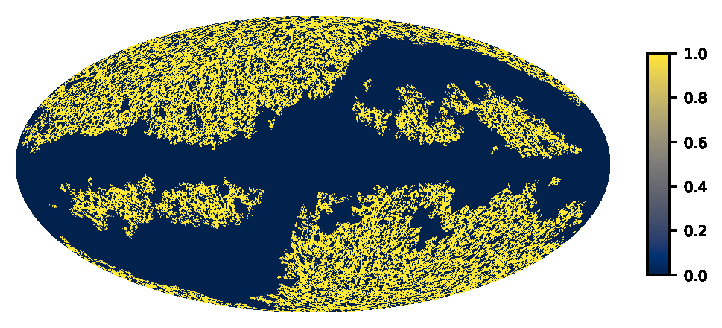
\includegraphics[width=.7\textwidth]{mask}
\caption{The Stage-IV-like mask describing a fictitious satellite-based survey used for the cut-sky results in this chapter.}
\label{bin_Fig:mask}
\end{figure}

For the cut-sky results, a Stage-IV-like mask describing a fictitious satellite-based survey was used. This was obtained by transforming the WMAP temperature mask used in \autoref{chap:exact_like} \citep{Bennett2013}, to excise the ecliptic plane in addition to the galactic plane. Additional point-source holes were added until a desired sky coverage of $\fsky = 0.3$ was achieved. The centre of each hole was chosen by selecting pixels at random. The immediate neighbouring pixels were also excised, after which a recursive probabilistic method was used, with a 50\% chance of the next neighbouring pixels being removed, and so on up to a maximum hole radius of 6 pixels. The final mask is shown in \autoref{bin_Fig:mask}.

The impact of the sky cut on observed power spectra was modelled using a mixing matrix obtained using \texttt{NaMaster} \citep{Alonso2019}. A cut-sky power spectrum covariance was obtained using the improved narrow kernel approximation \citep{Nicola2021} method described in \autoref{chap:cov}. The sky cut does not affect the expected value of the correlation function, but does affect its covariance. This is modelled by applying a factor of $1 / \fsky$ to the full-sky covariance matrix. Although this is presumably an approximation, it is standard practice for the cut-sky correlation function, used for example in the DES Year 3 covariance described in \citet{Friedrich2021}. It was shown in \citet{Cabre2007} that this `$\fsky$ approximation' is a good approximation to the simulated cut-sky correlation function covariance, which is not the case for the power spectrum. Nevertheless, in \autoref{bin_sec:fsky} it is shown that the use of this approximation for the power spectrum does not significantly affect the dependence of posterior uncertainties on the number of angular bins. Therefore, it can be expected to be a sufficiently accurate approximation for the correlation function in this chapter.

\subsection{Posterior uncertainty as a function of number of angular bins}
\label{bin_sec:results}

\begin{figure}[t]
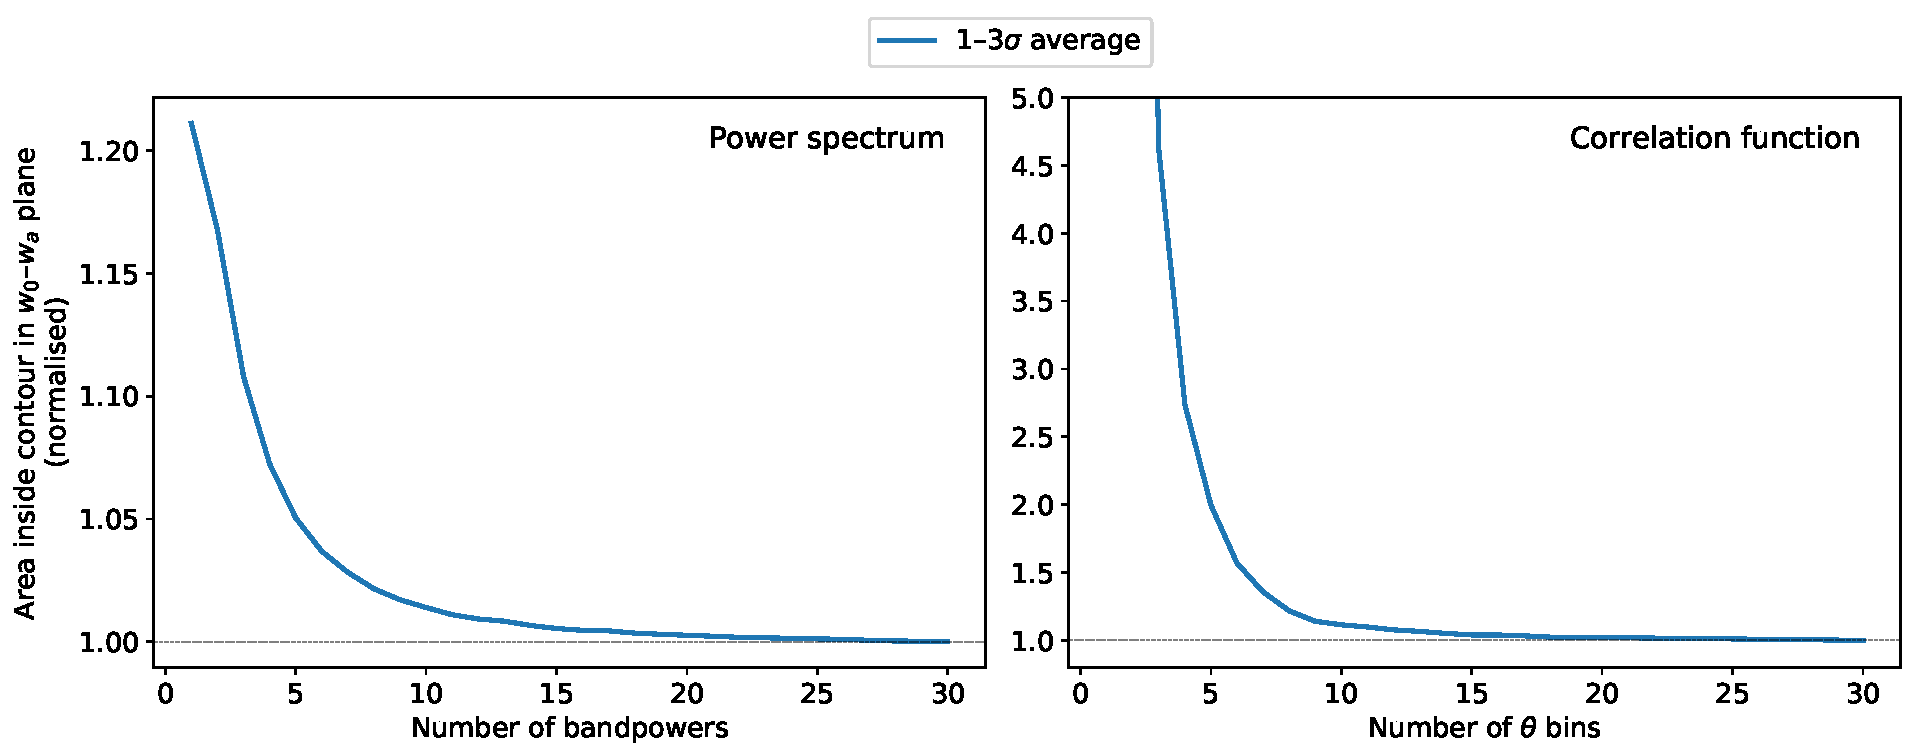
\includegraphics[width=\textwidth]{area_vs_nbin_fs}
\caption{Dependence of posterior uncertainties in a joint full-sky analysis of $w_0$ and $w_a$ on the number of angular bins for the power spectrum (left) and correlation function (right). Each line is averaged over 100 contours linearly spaced from $1\sigma$ to $3\sigma$ and normalised to be equal to 1 at its minimum, as described in the first paragraph of \autoref{bin_sec:results}.}
\label{bin_Fig:area_vs_nbin_fs}
\end{figure}

The dependence of posterior uncertainties in a joint full-sky analysis of $w_0$ and $w_a$ on the number of angular bins is shown for the power spectrum and correlation function in \autoref{bin_Fig:area_vs_nbin_fs}.
% Each line is averaged over 100 contours linearly spaced from $1\sigma$ to $3\sigma$ and normalised to be equal to 1 at its minimum.
Each line is calculated by forming the joint posterior distribution of $w_0$ and $w_a$, drawing 100 credible regions linearly spaced from $1\sigma$ to $3\sigma$ (following the definitions of credible regions and sigma notation described in \autoref{est_Sec:credible_regions_sigma_notation}), measuring the area of every credible region as a function of the number of angular bins, normalising each curve to be equal to 1 at its minimum, and finally averaging over all 100 regions. This technique removes most of the noise that results from the finite resolution of the posterior grids.

\begin{figure}[t]
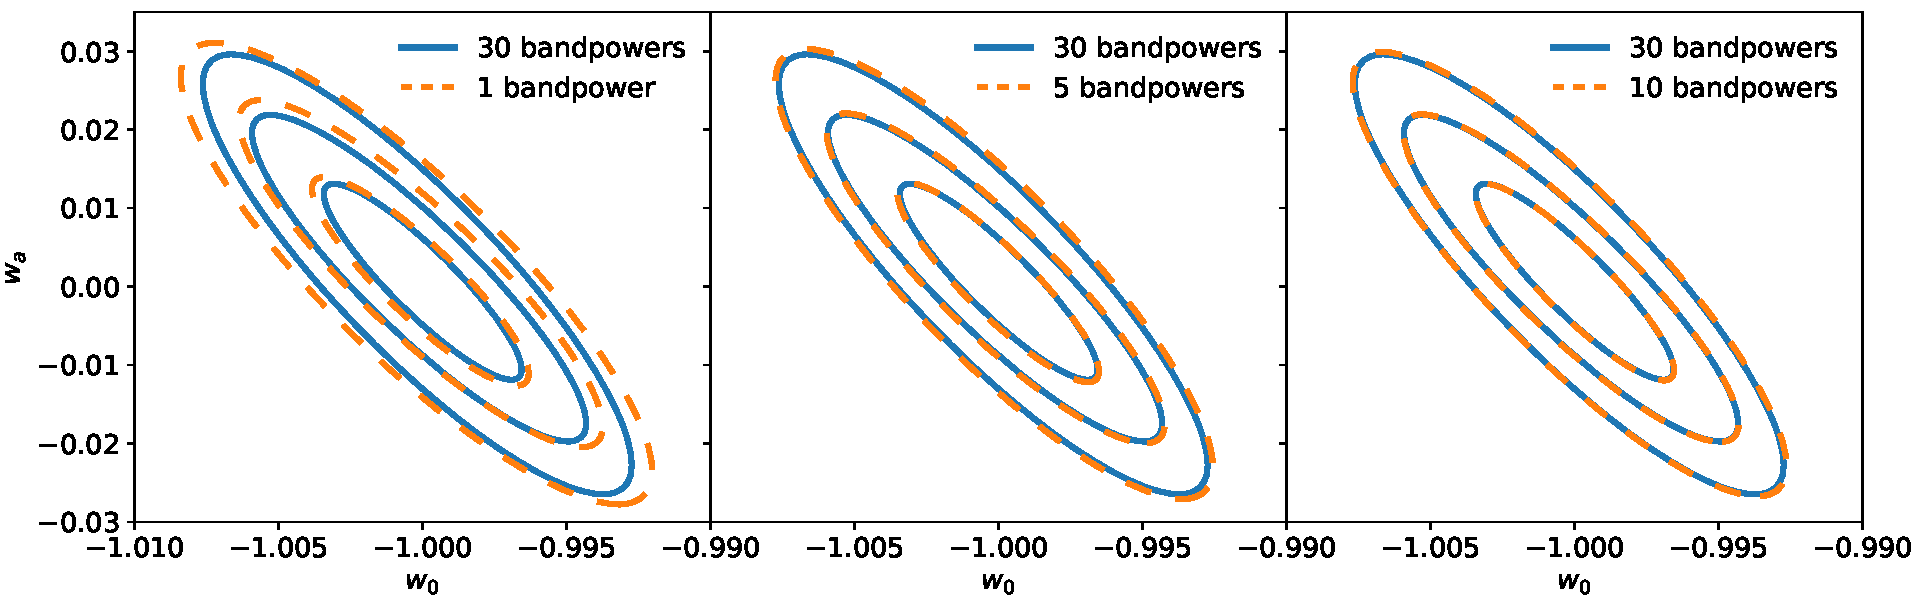
\includegraphics[width=\textwidth]{posts_w0wa_cl}
\caption{1--3$\sigma$ posterior contours from the full-sky power spectrum with different numbers of bandpowers used in the likelihood analysis.}
\label{bin_Fig:posts_w0wa_cl}
\end{figure}

\begin{figure}[t]
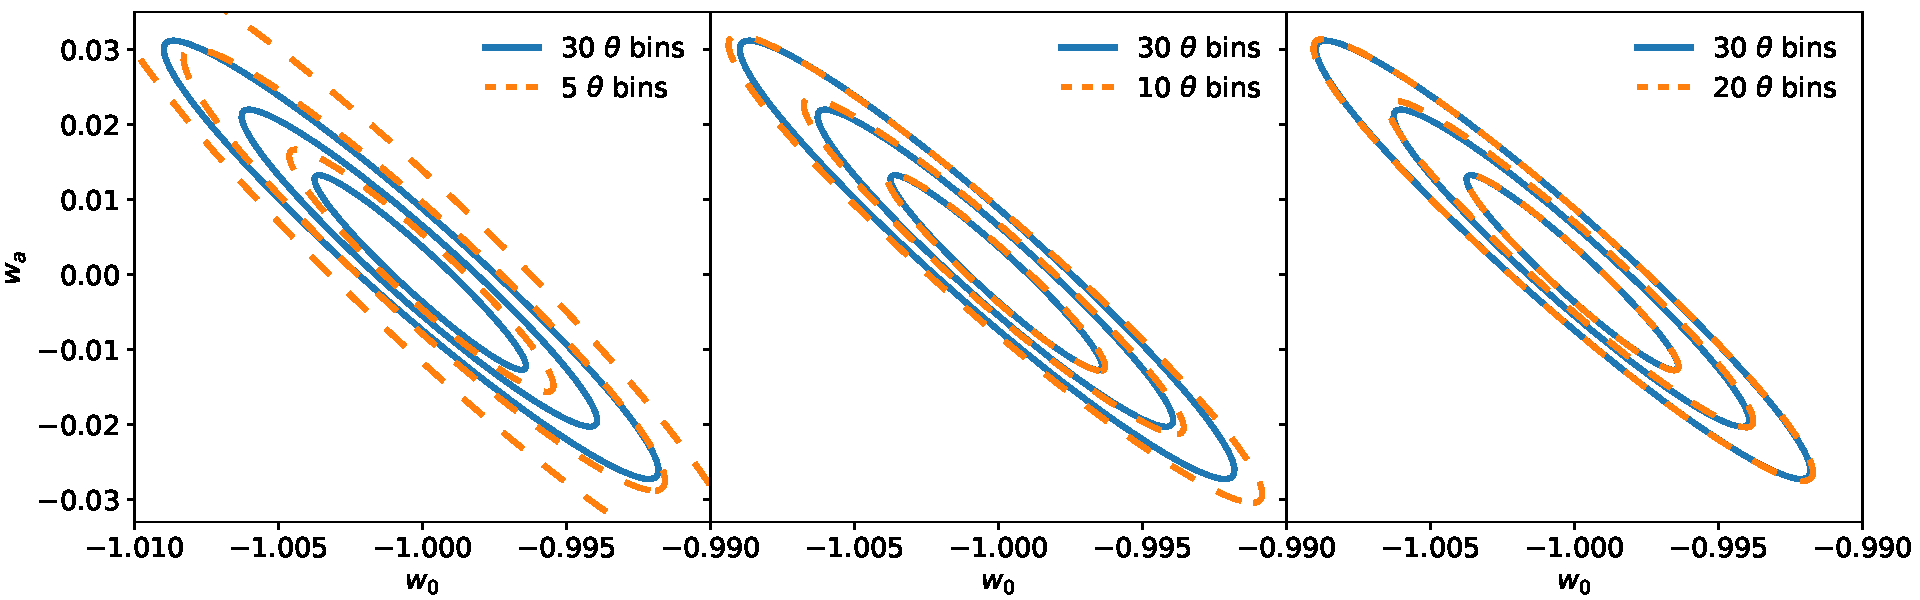
\includegraphics[width=\textwidth]{posts_w0wa_cf}
\caption{As \autoref{bin_Fig:posts_w0wa_cl} but for the correlation function. 1--3$\sigma$ posterior contours from the full-sky correlation function with different numbers of angular bins used in the likelihood analysis.}
\label{bin_Fig:posts_w0wa_cf}
\end{figure}

\begin{figure}[t]
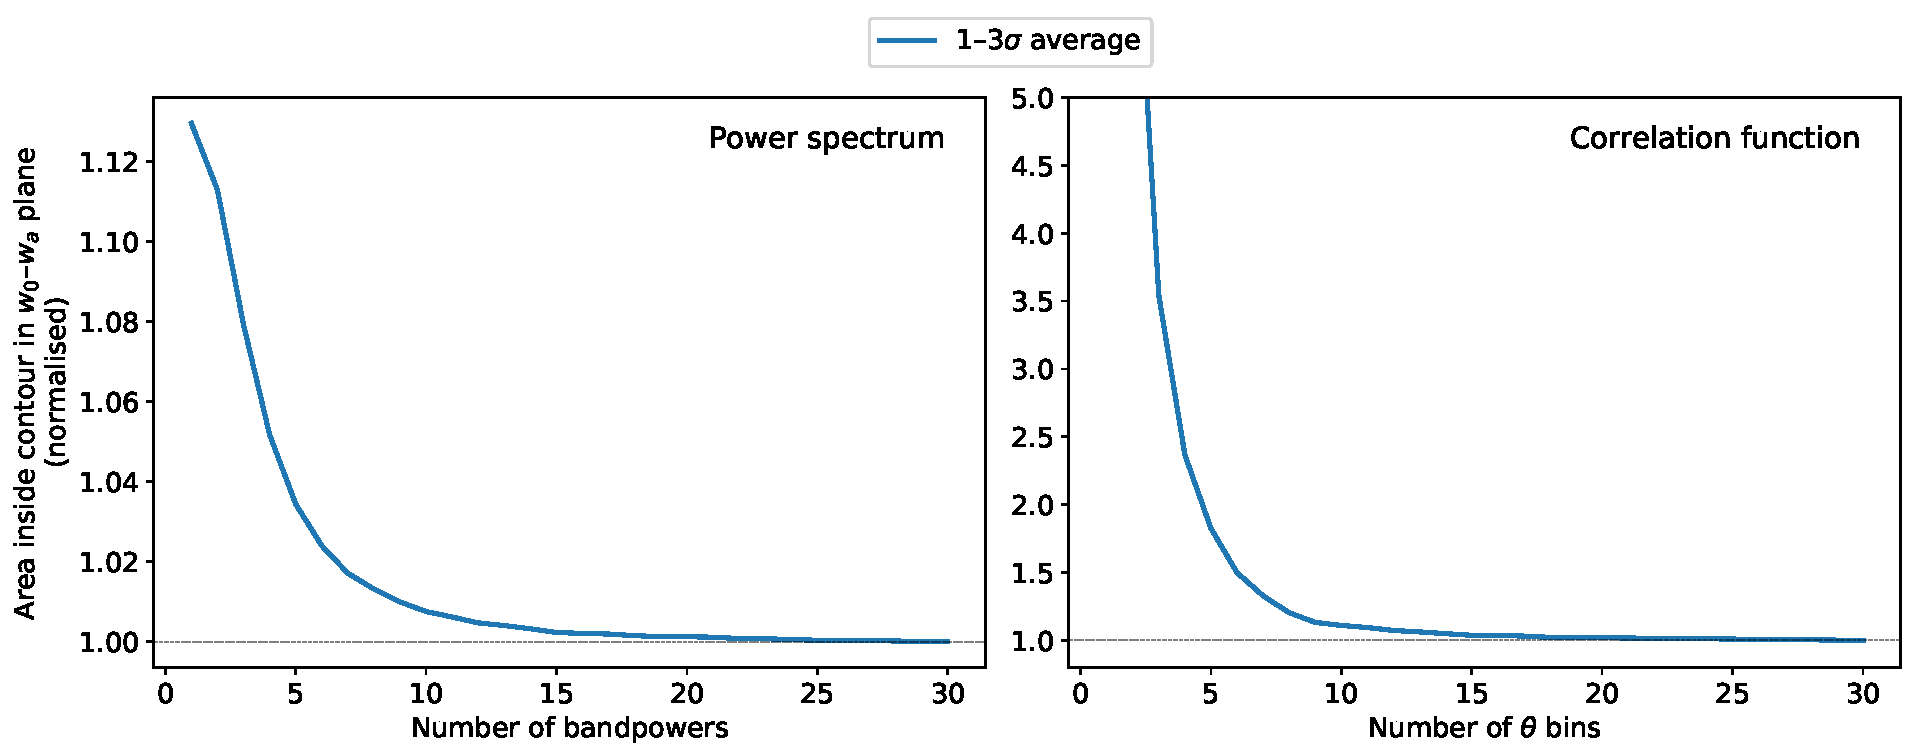
\includegraphics[width=\textwidth]{area_vs_nbin_ma}
\caption{As \autoref{bin_Fig:area_vs_nbin_fs} but for a cut-sky analysis. Dependence of posterior uncertainties in a joint cut-sky analysis of $w_0$ and $w_a$ on the number of angular bins for the power spectrum (left) and correlation function (right). Each line is averaged over 100 contours linearly spaced from $1\sigma$ to $3\sigma$ and normalised to be equal to 1 at its minimum, as described in the first paragraph of \autoref{bin_sec:results}.}
\label{bin_Fig:area_vs_nbin_ma}
\end{figure}

\begin{figure}[t!]
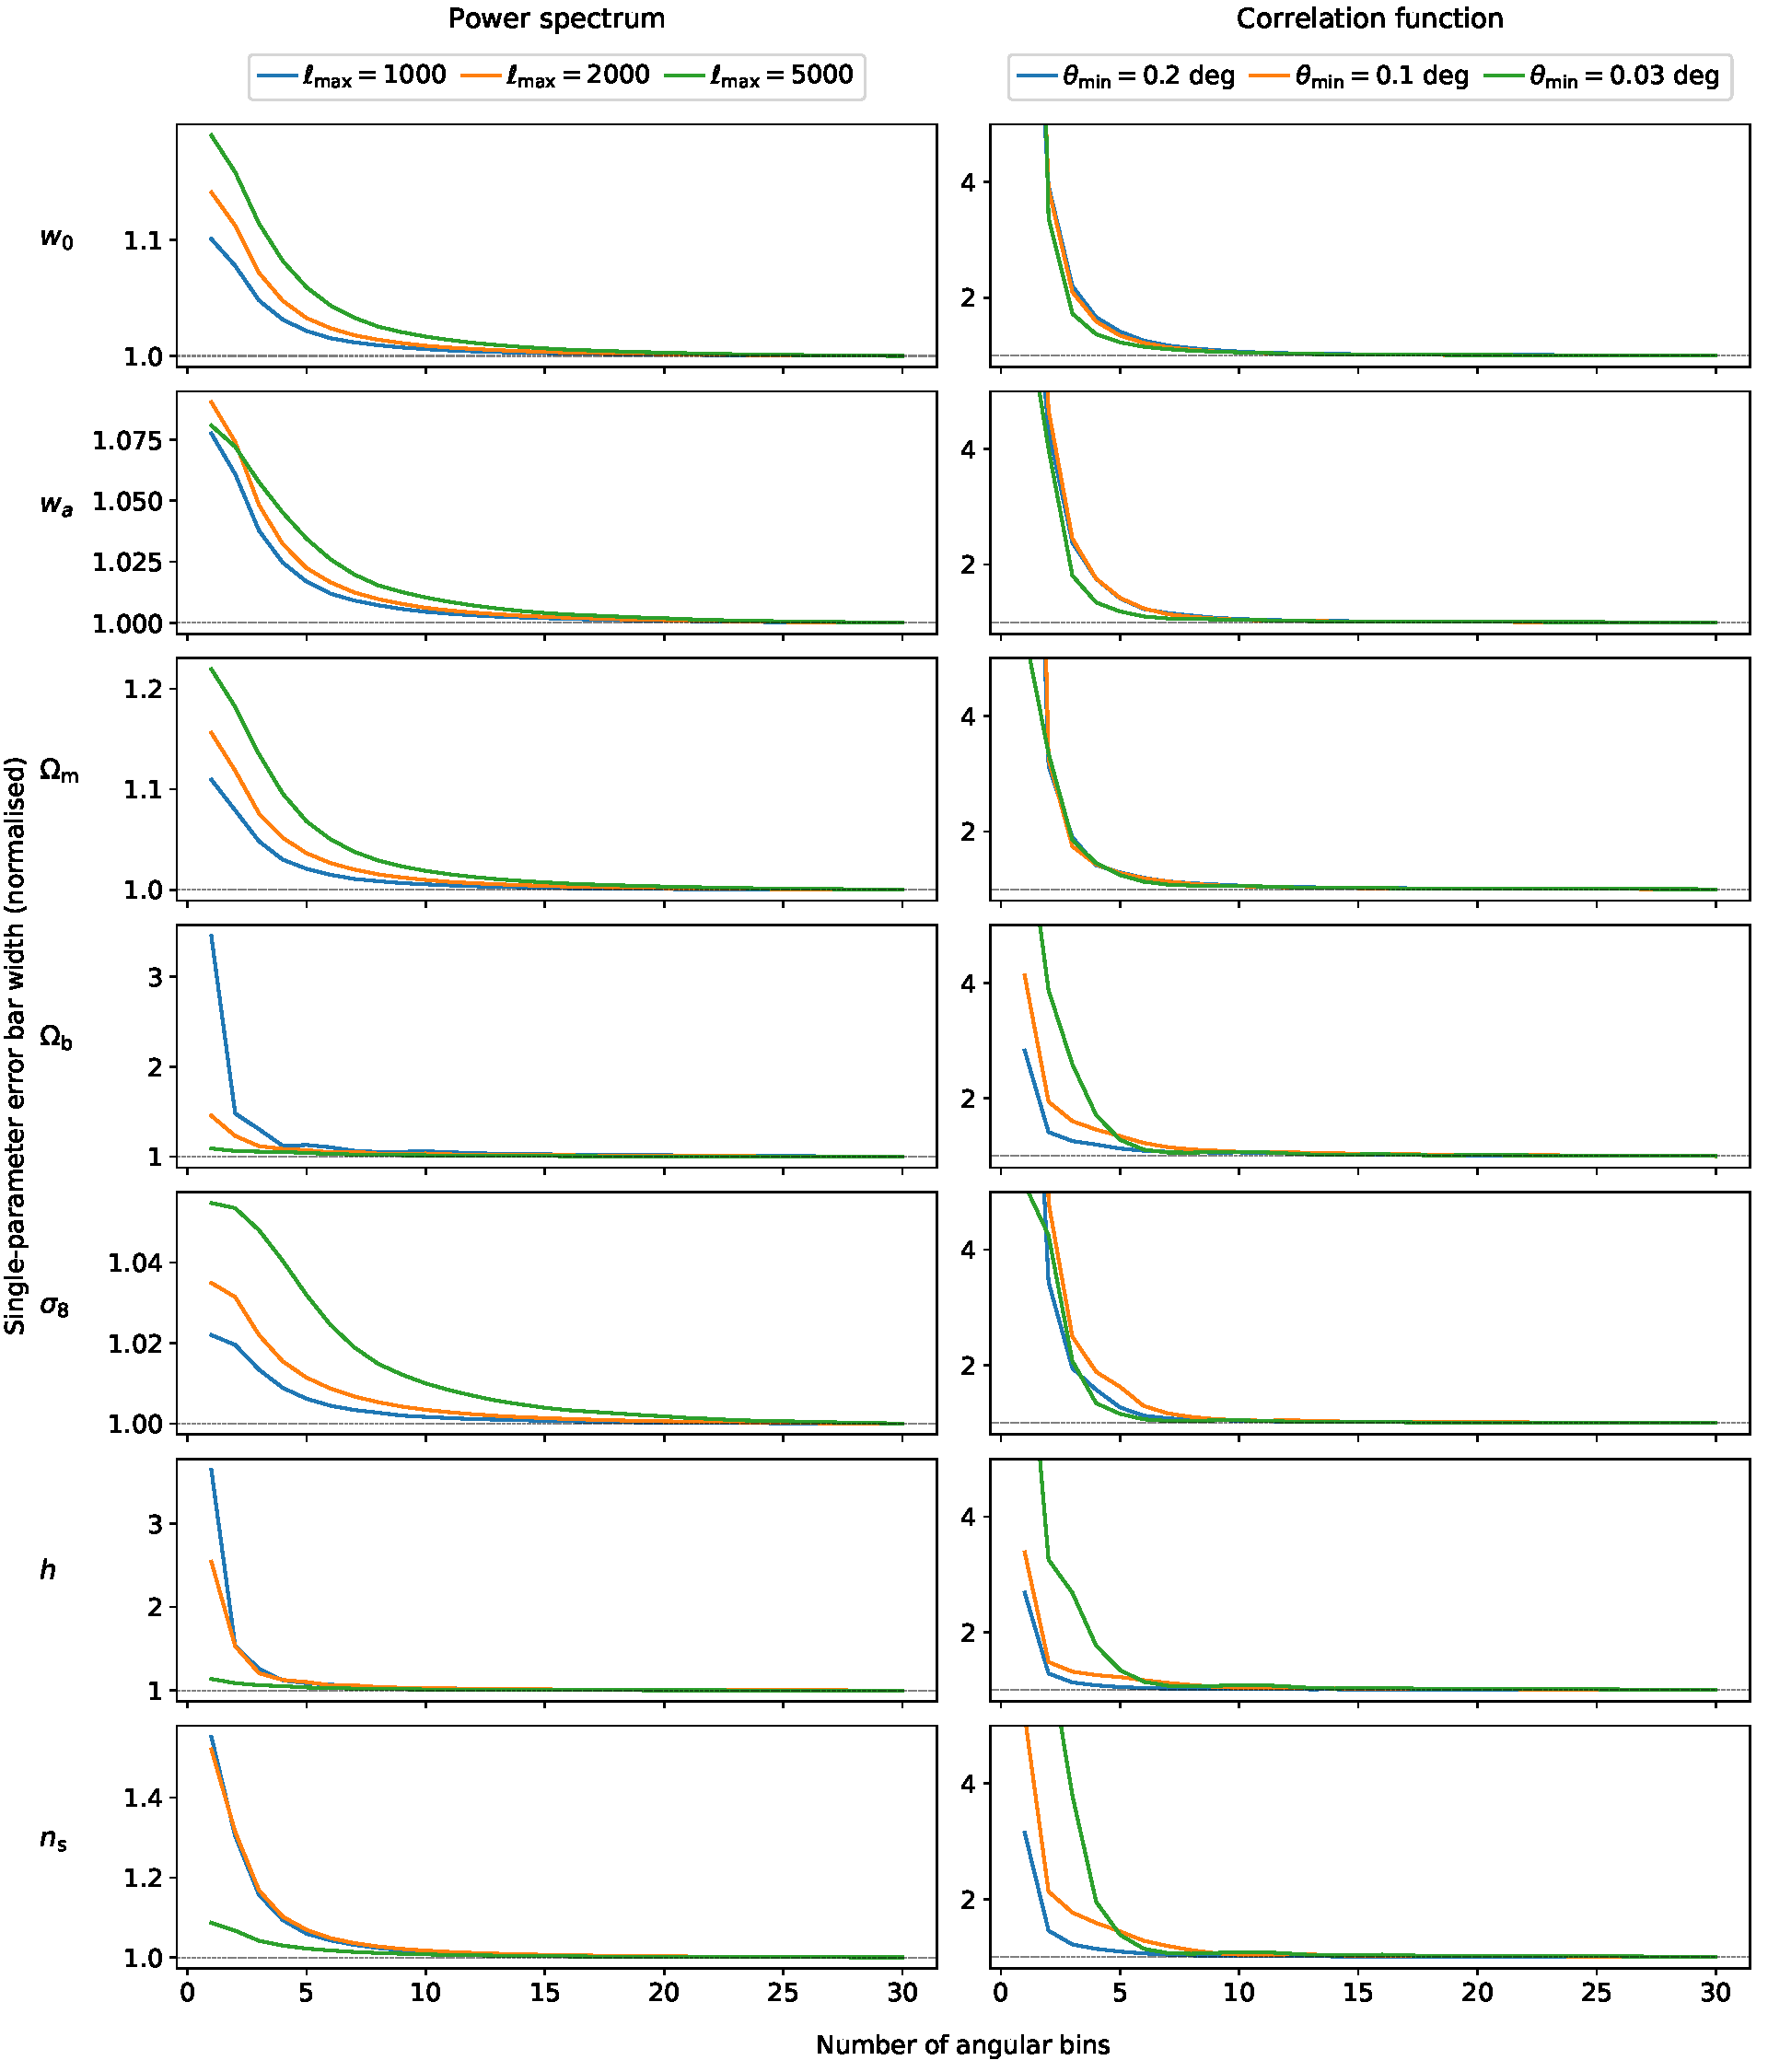
\includegraphics[width=\textwidth]{width_vs_nbin}
\caption{As \autoref{bin_Fig:area_vs_nbin_fs} but for a single parameter at a time. Dependence of posterior uncertainties in a single-parameter analysis on the number of angular bins for the power spectrum (left) and correlation function (right). Each line is averaged over 100 contours linearly spaced from $1\sigma$ to $3\sigma$ and normalised to be equal to 1 at its minimum, as described in the first paragraph of \autoref{bin_sec:results}. Each parameter is constrained independently, with all other parameters held fixed. The results for different scale cuts are shown in different colours.}
\label{bin_Fig:width_vs_nbin}
\end{figure}

Both lines in \autoref{bin_Fig:area_vs_nbin_fs} are mostly flat above around 10 angular bins, and converge to a minimum by around 20--25 bins. Below 10 bins, there is a sharp increase in contour area. For the power spectrum, however, this only reaches a maximum of around 20 per cent higher than the minimum area, even for a single bandpower. In contrast, the contour area for the correlation function diverges sharply at around 5 bins. This difference in behaviour is explored in \autoref{bin_sec:low_nbin}.

To further illustrate the dependence shown in \autoref{bin_Fig:area_vs_nbin_fs}, posterior distributions with different numbers of angular bins are shown in \autoref{bin_Fig:posts_w0wa_cl} for the full-sky power spectrum and in \autoref{bin_Fig:posts_w0wa_cf} for the full-sky correlation function. It can be seen in the left panel of \autoref{bin_Fig:posts_w0wa_cl} that the single-bandpower posterior distribution is only slightly larger than the equivalent result with 30 bandpowers. The correlation function posteriors in \autoref{bin_Fig:posts_w0wa_cf} show more degradation as the number of bins is decreased, as mentioned above.

\autoref{bin_Fig:area_vs_nbin_ma} shows the same dependence on the number of angular bins, but this time for a cut-sky analysis. The results are very similar to the full-sky results in \autoref{bin_Fig:area_vs_nbin_fs}. For this reason, the remainder of this chapter considers only a full-sky setup, but the conclusions should be applicable to a cut-sky analysis as well.

Additional cosmological parameters are investigated in \autoref{bin_Fig:width_vs_nbin}. These are chosen to be the parameters included in the \Euclid{} forecast paper \citep{Blanchard2020}: $w_0$, $w_a$, $\Omega_\text{m}$, $\Omega_\text{b}$, $\sigma_8$, $n_\text{s}$, $h$. These parameters are described in \autoref{chap:cosmo}. Each parameter is shown for three different scale cuts. For the power spectrum, the maximum multipole $\lmax$ is varied from the baseline value of $\lmax = 2000$ to a more conservative $\lmax = 1000$ and a more optimistic $\lmax = 5000$. For the correlation function, the respective equivalent minimum separation $\tmin$ values are $\tmin =$ 0.1\,deg, $\tmin =$ 0.2\,deg, and $\tmin =$ 0.03\,deg. While the different parameters behave broadly similarly, there are some differences. For example, while some parameters such as $w_0$ only exhibit a 10--20 per cent degradation at low numbers of bandpowers, others such as $\omb$ exhibit as much as 300 per cent degradation, perhaps because constraining such parameters requires sufficient angular resolution to resolve the shape of the power spectrum and not just its amplitude.

\begin{figure}[t]
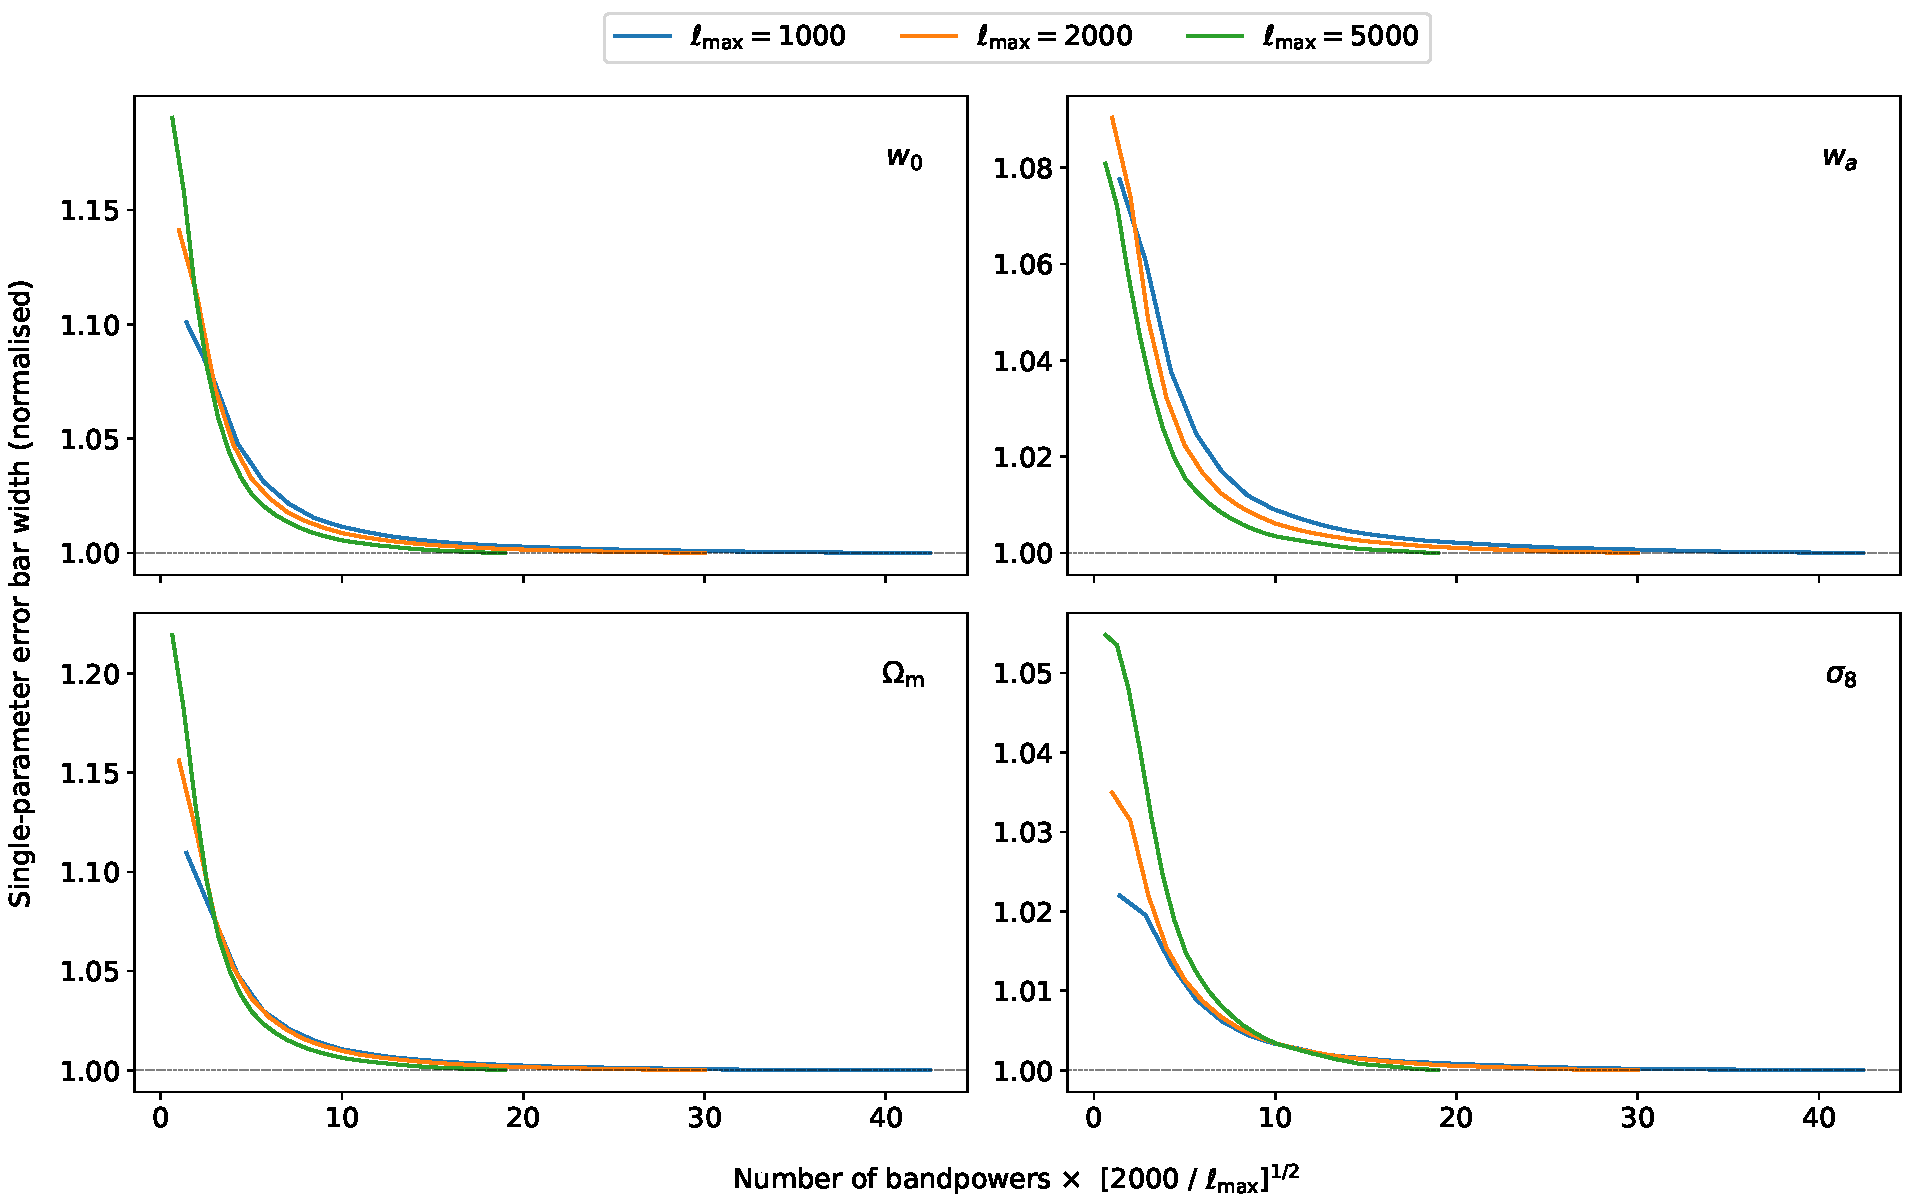
\includegraphics[width=\textwidth]{sqrt_lmax}
\caption{Dependence on the number of bandpowers for the full-sky power spectrum, for four parameters exhibiting a particular property: the number of bandpowers required for a particular level of degradation for different $\lmax$ values approximately scales as $\sqrt{\lmax}$.}
\label{bin_Fig:sqrt_lmax}
\end{figure}

Ideally it would be possible to unify the results with different scale cuts in \autoref{bin_Fig:width_vs_nbin} into a dependence on a single measure, such as the logarithmic angular bin size. However, the different parameters behave differently as $\lmax$ and $\tmin$ are varied, so this is not possible in practice. However, a certain subset of the parameters do exhibit such a convenient property for the power spectrum: it is shown in \autoref{bin_Fig:sqrt_lmax} that for four parameters---$\wo$, $\wa$, $\omm$ and $\sie$---the number of bandpowers required for a given $\lmax$ value scales approximately as $\sqrt{\lmax}$. The reason for this particular dependence is not clear, but it is perhaps not a coincidence that these parameters are those which depend most on the amplitude of weak lensing power spectra and least on their shape. For this reason, these parameters are also the most strongly correlated in a \Euclid{}-like analysis \citep{Blanchard2020}.

\section{Exploration of additional effects}
\label{bin_sec:additional_effects}

In this section, three different effects which may affect the required number of angular bins are explored. \autoref{bin_sec:fsky} investigates the impact of the $\fsky$ approximation in the power spectrum covariance. \autoref{bin_sec:low_nbin} explores why the power spectrum and correlation function exhibit such different behaviour for low numbers of angular bins, while \autoref{bin_Sec:noise} studies the impact of noise.

\subsection{Impact of \texorpdfstring{$\fsky$}{fsky} approximation}
\label{bin_sec:fsky}

\begin{figure}[t]
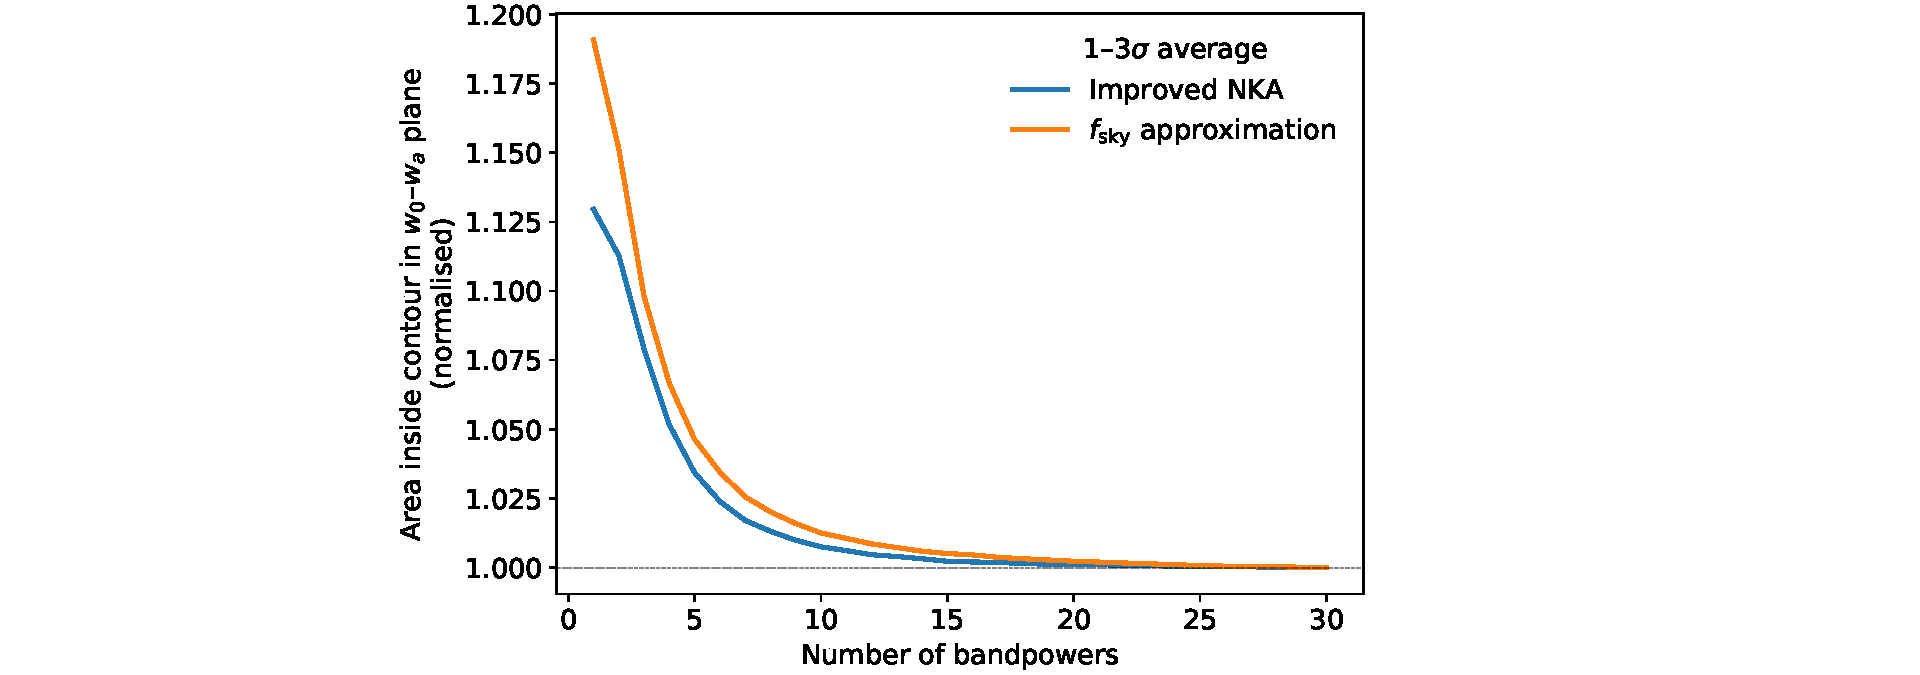
\includegraphics[width=\textwidth]{inka_vs_fsky}
\caption{Dependence of posterior uncertainties in a joint cut-sky analysis of $\wo$ and $\wa$ on the number of power spectrum bandpowers, when the covariance is calculated using the $\fsky$ approximation (\autoref{bin_eq:fsky_approx}) compared to the Improved NKA method. Each line is averaged over 100 contours linearly spaced from $1\sigma$ to $3\sigma$ and normalised to be equal to 1 at its minimum, as described in the first paragraph of \autoref{bin_sec:results}.}
\label{bin_Fig:inka_vs_fsky}
\end{figure}

In \autoref{bin_sec:main_analysis}, the cut-sky power spectrum covariance was calculated using the Improved NKA method. A faster alternative is to use the `$\fsky$ approximation':
\begin{equation}
\text{Cov}_\text{cut-sky} \approx \frac{1}{\fsky}
\text{Cov}_\text{full-sky},
\label{bin_eq:fsky_approx}
\end{equation}
where $\fsky$ is the observed fraction of the sky. \autoref{bin_Fig:inka_vs_fsky} shows the dependence of posterior uncertainties in a joint cut-sky analysis of $\wo$ and $\wa$ on the number of bandpowers when using the $\fsky$ approximation compared to the more accurate Improved NKA method.
% While not identical, the results are similar, except with only 1--2 angular bins.
While the curves produced by the two methods are not identical, the results are similar other than for a very coarse binning (1--2 angular bins).
The good performance of the $\fsky$ approximation for the power spectrum supports its use for the correlation function in \autoref{bin_sec:main_analysis}, especially when combined with the results of \citet{Cabre2007}, which show through a comparison with simulations that this approximation is much more accurate for the correlation function than it is for the power spectrum.

\subsection{Contrast between power spectrum and correlation function behaviour for small numbers of bins}
\label{bin_sec:low_nbin}

A peculiar result that occurs throughout \autoref{bin_sec:main_analysis} is that posterior uncertainties obtained through a power spectrum analysis tend to degrade much less for small numbers of angular bins than those obtained through a correlation function analysis. For example, in \autoref{bin_Fig:area_vs_nbin_fs}, even a single bandpower only returns a joint $\wo$--$\wa$ uncertainty around 20 per cent larger than with 30 bandpowers, whereas for the correlation function there is a sharp divergence by at least 500 per cent at around 5 angular bins. The explanation for this behaviour is the differing ways in which scales are weighted within each angular bin for the two methods, which will now be demonstrated.

\begin{figure}[t]
\includegraphics[width=\textwidth]{cl_perl}
\caption{Top: 45 theoretical power spectra, corresponding to the shear auto-power in the lowest redshift bin for different points in the $\wo$--$\wa$ plane. The points are chosen from a diagonal line running perpendicular to the $\wo$--$\wa$ degeneracy direction. Each model is coloured by its distance in $\sigma$ from the fiducial model, determined from a full-sky unbinned power spectrum likelihood analysis. In practice, the 45 power spectra all appear on top of one another. Error bars are shown at a selection of multipoles, and include a shape noise contribution. Bottom: The difference between each model and the fiducial model, scaled by the error bar for each $\ell$.}
\label{bin_Fig:cl_perl}
\end{figure}

The top panel of \autoref{bin_Fig:cl_perl} shows 45 theoretical power spectra, corresponding to the shear auto-power in the lowest redshift bin for different points in the $\wo$--$\wa$ plane. The points are chosen from a diagonal line running perpendicular to the $\wo$--$\wa$ degeneracy direction; that is, from the lower left to upper right of a given panel of \autoref{bin_Fig:posts_w0wa_cl}. Each model is coloured by its distance in $\sigma$ from the fiducial model, determined from a full-sky unbinned power spectrum likelihood analysis. The fiducial model is ($\wo$, $\wa$) = ($-1$, $0$). In practice, the 45 power spectra all appear on top of one another. Error bars are shown at a selection of multipoles, and include a shape noise contribution. In the lower panel, the difference between each model and the fiducial model is shown, scaled by the error bar for each $\ell$. This is effectively equivalent to the per-$\ell$ signal-to-noise as a function of scale. There is a region of very low signal-to-noise at low $\ell$, $\ell \lesssim 50$, which rapidly increases to a peak at around $\ell \sim 200$, followed by a gentle decrease towards higher $\ell$ as shape noise begins to dominate.

\begin{figure}[t]
\includegraphics[width=\textwidth]{cf_perbin}
\caption{As \autoref{bin_Fig:cl_perl} but for the correlation function. Top: 45 theoretical correlation functions, corresponding to $\xi^+$ in the lowest redshift bin for different points in the $\wo$--$\wa$ plane. The points are chosen from a diagonal line running perpendicular to the $\wo$--$\wa$ degeneracy direction. Each model is coloured by its distance in $\sigma$ from the fiducial model, determined from a full-sky unbinned power spectrum likelihood analysis. Error bars are shown for each angular bin, and include a shape noise contribution. Bottom: The difference between each model and the fiducial model, scaled by the error bar for each angular bin.}
\label{bin_Fig:cf_perbin}
\end{figure}

The equivalent for the correlation function, for $\xi^+$ in the lowest redshift bin, is shown in \autoref{bin_Fig:cf_perbin}. 30 angular bins are used. The colour for each model is the same as in \autoref{bin_Fig:cl_perl}. The signal-to-noise is roughly constant between 0.1 and 1 deg, before steadily decreasing to reach a very low level at 10 deg.

As seen in Figures \ref{bin_Fig:cl_perl} and \ref{bin_Fig:cf_perbin}, both the power spectrum and correlation function have poor signal-to-noise on large angular scales. This fact alone cannot explain the difference between them when small numbers of angular bins are used. The difference arises because of how scales are weighted within each bin. For the power spectrum, different $\ell$ within each bandpower are weighted as $\ell \left( \ell + 1 \right)$ following Equation \eqref{cov_eqn:pbl}, which quadratically downweights the largest scales, which are the lowest signal-to-noise part of the data vector. For the correlation function, however, different $\theta$ within each bin are weighted as $\sin{\theta}$, corresponding to a uniform distribution of galaxies \citep{Friedrich2021}. This weighting upweights the largest scales, which can dramatically decrease the signal-to-noise when combining scales into few bins.

\begin{figure}[tp]
\includegraphics[width=\textwidth]{cf_perbin_30vs15}
\caption{As \autoref{bin_Fig:cf_perbin}, but for 30 angular bins (left panel) compared to 15 (right panel).}
\label{bin_Fig:cf_perbin_30vs15}
\end{figure}

\begin{figure}[tp]
\includegraphics[width=\textwidth]{cf_perbin_2vs1}
\caption{As \autoref{bin_Fig:cf_perbin}, but for 2 angular bins (left panel) compared to 1 (right panel).}
\label{bin_Fig:cf_perbin_2vs1}
\end{figure}

The effect of the $\sin{\theta}$ weighting is small when relatively large numbers of angular bins are used. The left panel of \autoref{bin_Fig:cf_perbin_30vs15} shows the same selection of correlation functions and per-bin signal-to-noise for 30 angular bins, while the right panel uses 15 bins. Each angular bin on the right panel corresponds to exactly two bins on the left panel. It can be seen that the $\sin{\theta}$ weighting has little effect, because for instance the value of $\xi^+$ in the first bin in the right panel is approximately equal to the mean of the values of $\xi^+$ in the first two bins in the left panel. This is because with a fine binning such as that used here, the difference in $\sin{\theta}$ between adjacent bins is not significant.

However, with a very low number of bins the effect of the $\sin{\theta}$ weighting is large. \autoref{bin_Fig:cf_perbin_2vs1} shows the difference between using two angular bins in the left panel and just a single bin in the right panel. When combining the two bins into one, the value of $\xi^+$ is heavily weighted towards the larger-scale bin. The result is that the signal-to-noise drops by an order of magnitude, as is evident in the lower panels.

It is possible to demonstrate that the power spectrum would experience the same problem if large scales were not strongly downweighted. To do so, it is necessary to introduce a new technique, in order to combine the signal-to-noise across all angular bins while taking correlations between bins into account. This involves defining the covariance-weighted distance $d$,\footnote{This distance $d$ is equivalent to the Mahalanobis distance
\citep{Mahalanobis1936}.} as
\begin{equation}
d^2 = \left( \mathbf{x} - \mathbf{x}^\text{fid} \right)^\intercal
\mathbfss{\Sigma}^{-1}
\left( \mathbf{x} - \mathbf{x}^\text{fid} \right),
\label{bin_eq:cov_dist}
\end{equation}
where $\mathbf{x}$ is the theoretical data vector for a particular model (a set of $\Cl$ or $\xi \left( \theta \right)$ values), $\mathbf{x}^\text{fid}$ is the data vector predicted by the fiducial model, and $\mathbfss{\Sigma}$ is the covariance matrix.

\begin{figure}[tp]
\includegraphics[width=\textwidth]{dist_validation}
\caption{Comparison of the covariance-weighted distance $d$ defined in \eqref{bin_eq:cov_dist} to the distance from the fiducial model measured from the posterior distribution resulting from a full likelihood analysis, for each of 45 different models. Each model corresponds to a different point in the $\wo$-$\wa$ plane, selected from a diagonal line running perpendicular to the $\wo$--$\wa$ degeneracy direction. The dashed line represents equality.}
\label{bin_Fig:dist_validation}
\end{figure}

\autoref{bin_Fig:dist_validation} shows that Equation \eqref{bin_eq:cov_dist} correctly predicts the distance from the fiducial model measured from the posterior distribution resulting from a full likelihood analysis. The left panel shows the value of the covariance-weighted distance $d$ against the distance from the fiducial model in $\sigma$ measured from the posterior for the power spectrum, while the right panel shows it for the correlation function, for the selection of 45 models used throughout this section. The agreement is worse farther from the fiducial model, which may be a result of being close to the boundary of the prior region used in the likelihood analysis.

\begin{figure}[tp]
\includegraphics[width=\textwidth]{dist_weight}
\caption{Covariance-weighted distance $d$ from the fiducial model, as defined in Equation \eqref{bin_eq:cov_dist}, as a function of the number of angular bins, for a selection of 45 different models. Each model corresponds to a different point in the $\wo$-$\wa$ plane, selected from a diagonal line running perpendicular to the $\wo$--$\wa$ degeneracy direction. Each panel explores a different weighting of scales within each angular bin. Top left: power spectrum with the usual $\ell \left( \ell + 1 \right)$ weighting. Top right: correlation function with the $\sin{\theta}$ weighting corresponding to a uniform distribution of galaxies. Bottom left: power spectrum with a flat weighting, where each $\ell$ is weighted equally within each bandpower. Bottom right: power spectrum with a correlation-function-like $\sin{\left( \pi / \ell \right)}$ weighting.}
\label{bin_Fig:dist_weight}
\end{figure}

The upper left panel of \autoref{bin_Fig:dist_weight} shows the covariance-weighted distance from the fiducial model as a function of the number of angular bins for the power spectrum with the usual $\ell \left( \ell + 1 \right)$ weighting, for each of the 45 models. The results are consistent with those found from a full likelihood analysis in \autoref{bin_Fig:area_vs_nbin_fs}: the distance at which each model is excluded only decreases slightly when reducing the number of bandpowers, even to a single bandpower. The upper right panel shows the equivalent for the correlation function, which is weighted within each bin as $\sin{\theta}$. As seen previously in \autoref{bin_Fig:area_vs_nbin_fs}, there is a much more severe degradation in performance for small numbers of bins, with the distance from the fiducial model shrinking to approximately zero for a model excluded at more than 30$\sigma$ with 20--30 angular bins.

The lower left panel of \autoref{bin_Fig:dist_weight} shows the effect of applying a flat weighting to the power spectrum; that is, weighting each $\ell$ equally within a given bandpower. The effect here is to reduce the amount by which large scales are downweighted, which leads to a degradation in the overall signal-to-noise for small numbers of bandpowers. Finally, in the lower right panel, a weighting is applied that is equivalent to the way in which the correlation function is weighted: each $\ell$ is weighted as $\sin{\left( \pi / \ell \right)}$. The resulting form of the distance from the fiducial model as a function of the number of bins is almost identical to that for the correlation function. This demonstrates that the weighting of scales within bins is responsible for the different behaviour of the power spectrum and the correlation function for low numbers of angular bins.

\subsection{Impact of noise}
\label{bin_Sec:noise}

It is possible that the results derived in the main analysis presented in \autoref{bin_sec:main_analysis} may vary if the level of noise present in the data changes. This is investigated in this section.

\begin{figure}[tp]
\includegraphics[width=\textwidth]{width_vs_noise}
\caption{Dependence of $\wo$ posterior uncertainty on the number of angular bins for the power spectrum and correlation function, for three different noise levels. Top: power spectrum, varying noise by a factor of 100. Lower left: power spectrum, varying noise by a factor of 2. Lower right: correlation function, varying noise by a factor of 2. Each line is averaged over 100 contours linearly spaced from $1\sigma$ to $3\sigma$ and normalised to be equal to 1 at its minimum, as described in the first paragraph of \autoref{bin_sec:results}. The baseline noise level corresponds to 30 galaxies\,/\,arcmin${}^2$ across all redshift bins.}
\label{bin_Fig:width_vs_noise}
\end{figure}

The top panel of \autoref{bin_Fig:width_vs_noise} shows the posterior uncertainty in $\wo$ from a full-sky power spectrum analysis, as a function of the number of bandpowers, for three noise levels. The baseline noise level corresponds to 30 galaxies\,/\,arcmin${}^2$ across all redshift bins, while the line labelled `$\times$100 noise' corresponds to 0.3\,/\,arcmin${}^2$ and the line labelled `$\times$0.01 noise' corresponds to 3000\,/\,arcmin${}^2$. Different behaviour is observed for the three different noise levels, which is discussed further below. Varying the noise by a factor 100 turned out to not be possible for the correlation function, due to problems with the conditioning of the covariance matrix for low noise levels. For a fair comparison with the correlation function, the lower left panel therefore shows the results for power spectrum with the noise varying by a factor of 2. `$\times$2 noise' corresponds to 15 galaxies\,/\,arcmin${}^2$, while `$\times$0.5 noise' corresponds to 60\,/\,arcmin${}^2$. While the spacing between the three lines is smaller than in the top panel, it is still clearly present in the same arrangement.

The right panel of \autoref{bin_Fig:width_vs_noise} shows the equivalent figure for the correlation function, with a factor of 2 between each noise level. In this case, little clear difference is observed between the different noise levels.

Insight into the different behaviour of the power spectrum and correlation function under varying noise levels seen in \autoref{bin_Fig:width_vs_noise} may be gained by studying the signal-to-noise as a function of scale for each method with an enhanced level of noise. This may be studied using some of the methods developed in \autoref{bin_sec:low_nbin} above. Since the methods used here do not require the use of a covariance matrix, a factor of 100$\times$ may be used without any problems, which allows a clearer illustration of the effect of noise.

The lower panel of \autoref{bin_Fig:cl_perl_x100noise} shows the per-$\ell$ signal-to-noise of the shear auto-power spectrum in the lowest redshift bin for the 100$\times$ baseline noise level. (See \autoref{bin_sec:low_nbin} for a more detailed explanation of this type of figure.) In contrast to the relatively small drop in signal-to-noise towards higher $\ell$ seen in \autoref{bin_Fig:cl_perl}, there is now a much larger decrease, in addition to a shift in the peak towards lower $\ell$ ($\ell \sim 50$). This is because the smaller scales are heavily suppressed by the increased noise level. If these low signal-to-noise small scales are combined in a single bin with the high signal-to-noise region, they will be strongly upweighted by the $\ell \left( \ell + 1 \right)$ weighting of $\ell$s within bandpowers, leading to a strong decrease in the overall signal-to-noise. This is what is observed in the `$\times$100 noise' line in the top panel of \autoref{bin_Fig:width_vs_noise}, and to a smaller extend in the `$\times$2 noise' line in the lower left panel of the same figure. The opposite effect can be expected to occur for low noise levels, which can explain the shallow slope of the `$\times$0.01 noise' and `$\times$0.5 noise' lines.

\begin{figure}[tp]
\includegraphics[width=\textwidth]{cl_perl_x100noise}
\caption{As \autoref{bin_Fig:cl_perl} but with 100$\times$ baseline noise. Top: 45 theoretical power spectra, corresponding to the shear auto-power in the lowest redshift bin for different points in the $\wo$--$\wa$ plane. The points are chosen from a diagonal line running perpendicular to the $\wo$--$\wa$ degeneracy direction. Each model is coloured by its distance in $\sigma$ from the fiducial model, determined from a full-sky unbinned power spectrum likelihood analysis. In practice, the 45 power spectra all appear on top of one another. Error bars are shown at a selection of multipoles, and include a shape noise contribution. Bottom: The difference between each model and the fiducial model, scaled by the error bar for each $\ell$.}
\label{bin_Fig:cl_perl_x100noise}
\end{figure}

\begin{figure}[tp]
\includegraphics[width=\textwidth]{cf_perbin_x100noise}
\caption{As \autoref{bin_Fig:cf_perbin} but with 100$\times$ baseline noise. Top: 45 theoretical correlation functions, corresponding to $\xi^+$ in the lowest redshift bin for different points in the $\wo$--$\wa$ plane. The points are chosen from a diagonal line running perpendicular to the $\wo$--$\wa$ degeneracy direction. Each model is coloured by its distance in $\sigma$ from the fiducial model, determined from a full-sky unbinned power spectrum likelihood analysis. Error bars are shown for each angular bin, and include a shape noise contribution. Bottom: The difference between each model and the fiducial model, scaled by the error bar for each angular bin.}
\label{bin_Fig:cf_perbin_x100noise}
\end{figure}

\autoref{bin_Fig:cf_perbin_x100noise} shows the equivalent for the correlation function. Compared to the baseline noise level seen previously in \autoref{bin_Fig:cf_perbin}, there is little change in shape when the noise is increased. This is unlike the power spectrum, and explains why the dependence on the number of correlation function bins sees little change when the noise level is varied.

\section{Conclusions}
\label{bin_sec:conclusions}

This chapter has investigated the question of how the statistical uncertainties in the posterior distributions of cosmological parameters derived from weak lensing two-point statistics depend on the number of angular bins used in the analysis. In \autoref{bin_sec:main_analysis} it was shown that for some parameters such as $\wo$ and $\wa$, these uncertainties for the power spectrum only increase by 7--20 per cent even for a single bandpower, relative to 30 bandpowers. In contrast, for the correlation function there is a sharp divergence by several hundred per cent at around 5 angular bins. However, these results vary quite substantially depending on the parameters in question and other aspects of the analysis. For example, power spectrum constraints in $\omb$ and $h$ can degrade by over 200 per cent for low numbers of bandpowers, while the same parameters do not suffer quite as badly for the correlation function. There is an inconsistent dependence on scale cut: a selection of four cosmological parameters ($\wo$, $\wa$, $\omm$, $\sie$) exhibit a dependence of $\sqrt{\lmax}$ for the power spectrum, but not for the correlation function, while the other parameters investigated ($\omb$, $h$, $n_s$) show no such dependence.

In \autoref{bin_sec:additional_effects} a number of additional effects have been investigated. It was shown in \autoref{bin_sec:fsky} that the use of the `$\fsky$ approximation' for the power spectrum covariance leads to similar results to using the full Improved NKA method. The different behaviour of the power spectrum and correlation function for small numbers of bins was investigated in \autoref{bin_sec:low_nbin}, where it was shown that this arises from the different ways in which scales are weighted within each angular bin. Finally, the effect of noise was studied in \autoref{bin_Sec:noise}, where it was shown that the number of angular bins needed for the correlation function has no strong dependence on the level of noise, but that a higher noise level in the power spectrum requires more bandpowers.

While there is no single rule for the number of required angular bins that captures all possible analysis setups, the results in this chapter suggest that, for instance, if a maximum degradation on parameter uncertainties of 10 per cent is required, then 10 bandpowers appears comfortably sufficient for power spectra, and 15 angular bins for correlation functions. This is true for any angular range up to at least $\lmax = 5000$ ($\tmin = 0.03\,\text{deg}$), although significantly higher scale cuts than this may require more bins.


% % Uncomment to build alone without subfiles:
% \emergencystretch=.4em % to avoid overfull hboxes
% \printbibliography[heading=bibintoc]
% \end{document}


% Weak lensing estimation with convolutional neural networks

% % Uncomment to build this alone without subfiles:
% % (also stuff at bottom)
% \documentclass{scrbook}
% % Koma script document options
\KOMAoption{paper}{a4}
\KOMAoption{fontsize}{11pt}
\KOMAoption{parskip}{half-} % paragraph spacing
% \KOMAoption{numbers}{enddot} % dot after section number
\KOMAoption{cleardoublepage}{plain} % include page numbers on blank pages
\KOMAoption{chapterprefix}{true} % 'Chapter' before number

% Packages
\usepackage{amsmath} % Gives \text command inside maths blocks
\usepackage{amssymb} % Various maths symbols
\usepackage{array} % Table formatting
\usepackage{bm} % Bold maths including Greek
\usepackage[format=plain]{caption} % Font sizing and alignment in captions
\usepackage{enumitem} % Allows numbering like 1.1 in ordered lists
% \usepackage{float} % Allows H placement of floats
\usepackage{graphicx}
\usepackage[hidelinks]{hyperref} % Hyperlinks without looking like it
% \usepackage{longtable} % Multi-page tables
% \usepackage{multicol} % For columns in text (not tables)
\usepackage{multirow} % For tables
\usepackage{neuralnetwork} % Neural net diagram
\usepackage{pdflscape} % Gives landscape environment
% \usepackage{scrlayer-scrpage} % To move page numbers
\usepackage{tabularx}
\usepackage{textcomp} % Added to fix \textasciiacute error on laptop
% \usepackage{tikz} % Diagrams (used for neural network example)
% \usepackage[pagenumberwidth=3em]{tocbasic}
% \usepackage{tocstyle} % ToC styling
\usepackage{upgreek} % Non-italic greek letters
\usepackage{xpatch} % Biblatex customisation

\usepackage[a4paper, inner=40mm, outer=15mm, top=30mm, bottom=30mm,footskip=15mm, headsep=15mm]{geometry}
% \usepackage[a4paper, inner=40mm, outer=30mm, top=50mm, bottom=50mm,footskip=20mm, headsep=20mm]{geometry} % footskip is space between footer (i.e. page number) and bottom of text
% min allowed is inner 40 mm, others 15 mm

\pagestyle{plain} % no header for front matter, overridden at end of front matter

% Caption setup
% \tablecaptionabove
\captionsetup[table]{labelsep=space}
% \captionsetup[table]{labelsep=space, skip=50pt, position=top}
\captionsetup[figure]{labelsep=space} % labelsep prevents dot followed by colon in captions

% Line spacing
\usepackage{setspace}
% \setstretch{1.4} % strangely this is > \onehalfspacing but < \doublespacing
\onehalfspacing
% \doublespacing

\raggedbottom % prevent huge spaces between paragraphs

% % % % % % % % % % % % % % % % % % % % % % % % %
% Font setup
% \usepackage{mathpazo} % Covers maths mode too
\usepackage[sc]{mathpazo} % Covers maths mode too, sc enables small caps
% \usepackage{palatino}
\usepackage[T1]{fontenc} % 8-bit font encoding
\addtokomafont{disposition}{\rmfamily} % Use serif throughout
% % % % % % % % % % % % % % % % % % % % % % % % %

% % % % % % % % % % % % % % % % % % % % % % % % %
% Section formatting setup
% \RedeclareSectionCommand[beforeskip=0pt]{chapter}
\RedeclareSectionCommand[beforeskip=0pt, innerskip=0pt]{chapter}
\RedeclareSectionCommand[beforeskip=10pt]{subsubsection}
\RedeclareSectionCommand[afterskip=1pt]{subsubsection}
% \setcounter{secnumdepth}{\subsubsectionnumdepth} % number up to subsubsections

% No dot after chapter number (https://tex.stackexchange.com/a/484727)
\renewcommand*{\chapterformat}{%
  \mbox{\chapappifchapterprefix{\nobreakspace}\thechapter
  \IfUsePrefixLine{}{\enskip}}%
}

% In the running header, separate chapter number and name with em dash
\renewcommand*{\chaptermarkformat}{%
\chapapp~\thechapter~---~}

% Create subsubsubsection below subsubsection but above paragraph, following https://tex.stackexchange.com/a/356574

\DeclareNewSectionCommand[
  style=section,
  counterwithin=subsubsection,
  afterskip=1pt,
  beforeskip=10pt,
  % afterskip=1.5ex plus .2ex,
  % beforeskip=3.25ex plus 1ex minus .2ex,
  % afterindent=false,
  level=\paragraphnumdepth,
  tocindent=10em,
  tocnumwidth=5em
]{subsubsubsection}
\setcounter{secnumdepth}{\subsubsubsectionnumdepth}
% \setcounter{tocdepth}{\subparagraphtocdepth}
\setcounter{tocdepth}{\subsubsubsectionnumdepth}

\RedeclareSectionCommands[
  level=\numexpr\subsubsubsectionnumdepth+1\relax,
  toclevel=\numexpr\subsubsubsectiontocdepth+1\relax,
  increaselevel,
]{paragraph,subparagraph}
\RedeclareSectionCommand[
  counterwithin=subsubsubsection,
  tocindent=12em,
  tocnumwidth=6em,
  beforeskip=10pt,
  afterskip=1pt, % line break after paragraph title
]{paragraph}
\RedeclareSectionCommand[
  tocindent=14em,
  tocnumwidth=7em,
  beforeskip=0pt
]{subparagraph}
% % % % % % % % % % % % % % % % % % % % % % % % %

% Autoref capitalisation
\def\chapterautorefname{Chapter}
\def\sectionautorefname{Section}
\def\subsectionautorefname{Section}
\def\subsubsectionautorefname{Section}

% % % % % % % % % % % % % % % % % % % % % % % % %
% Bibliography setup
\usepackage[backend=biber,
    % style=authoryear,
    style=authoryear-comp, % Don't repeat same author(s) in multiple citations
    giveninits=true,
    useprefix=true, % 'van der' etc.
    url=false,
    doi=false,
    isbn=false,
    eprint=false,
    uniquename=false, % Don't add initials in citation to disambiguate between authors with the same surname
    uniquelist=false, % Don't disambiguate in citation between different 'et al.' teams
    maxbibnames=10,
    minbibnames=10,
    maxcitenames=3,%  # 2,
    natbib, % Gives citep and citet commands
    labelalpha=true, % Use an 'alpha' label for each bib entry
    maxalphanames=1, % Use first author as the alpha label
    sorting=anyvt, % Sort by alpha (first author) then year
    block=par, % New line between 'blocks' of the bib entry
    dashed=false, % Reprint author list for each publication in bibliography
    sortcites=false % Show citations in the order supplied
]{biblatex}

% Citation/reference parameters
\renewcommand*{\nameyeardelim}{\addspace} % Space between author and year rather than comma
\renewcommand*{\finalnamedelim}{\addspace\&\addspace} % Ampersand rather than 'and'
\xpatchbibmacro{name:andothers}{{\finalandcomma}}{\addspace}{}{} % Space before 'et al.' rather than comma

% Citation-specific parameters
\DeclareCiteCommand{\blindcite}{\unspace}{}{}{\mancite} % Easy manual citations

% Reference-specific parameters
\AtEveryBibitem{\clearfield{title}} % Suppress title
\AtEveryBibitem{\clearfield{month}} % Suppress month
\DeclareNameAlias{author}{family-given} % Surname first for not just the first author
\DeclareNameAlias{editor}{family-given} % Same for editors
\renewbibmacro{in:}{} % Remove 'In:'
\DeclareFieldFormat{journaltitle}{#1} % Journal title in normal font rather than italics
\renewbibmacro*{volume+number+eid}{\printfield{volume}\printfield{number}\setunit{\addcomma\space}\printfield{eid}} % No dot after issue
\DeclareFieldFormat[article]{number}{\mkbibparens{#1}} % Volume in brackets
\DefineBibliographyStrings{english}{page = {}, pages = {}} % Suppress 'p.'/'pp.'
\renewbibmacro*{date+extradate}{\printtext{\printfield{year}\addcomma}} % Year not in brackets
\DeclareFieldFormat{pages}{\mkfirstpage[{\mkpageprefix[bookpagination]}]{#1}} % Only give starting page
\DeclareFieldFormat{url}{\url{#1}} % No 'URL' before URLs
% \renewcommand{\finentrypunct}{} % Remove final full stop
\renewcommand*{\newunitpunct}{\addcomma\space} % Commas between elements of bibitems

\DeclareBibliographyDriver{book}{%
  \printnames{author}%
  \space
  \printfield{year}%
  \newunit\newblock
  \printfield{booktitle}%
  \newunit
  , \printlist{publisher}%
\finentry}

\DeclareBibliographyDriver{inproceedings}{%
  \printnames{author}%
  \space
  \printfield{year}%
  \newunit\newblock
  \printfield{booktitle}%
  \newunit
  \printfield{volume}%
  \newunit
  \printfield{pages}%
\finentry}

\DeclareBibliographyDriver{incollection}{%
  \printnames{author}%
  \space
  \printfield{year}%
  \newunit\newblock
  \printfield{booktitle}%
  \newunit
  , ed. \printnames{editor},%
  \newunit\newblock
  \printlist{publisher}%
\finentry}

\DeclareBibliographyDriver{misc}{%
  \printnames{author}%
  \space
  \printfield{year}%
  \newunit\newblock
  \printfield{title}%
  \newunit
  \printfield{url}%
\finentry}

\addbibresource{refs.bib}
% % % % % % % % % % % % % % % % % % % % % % % % %

% Footnote spacing
% \deffootnote[1em]{1.5em}{1em}{\textsuperscript{\thefootnotemark~}}
\deffootnote[1em]{1em}{1em}{\textsuperscript{\thefootnotemark~}}

% Testing setting all penalties to zero
\binoppenalty=0
\brokenpenalty=0
\clubpenalty=0
\displaywidowpenalty=0
\exhyphenpenalty=0
\floatingpenalty=0
\hyphenpenalty=0
\interlinepenalty=0
% \linepenalty=0 % allowing this to be zero splits titles in a strange way
\postdisplaypenalty=0
\predisplaypenalty=0
\relpenalty=0
\widowpenalty=0

% Shorthands (non-Maths)
\newcommand{\lcdm}{$\Lambda$CDM}
\newcommand{\wcdm}{$w$CDM}
\newcommand{\Euclid}{\textit{Euclid}}
\newcommand{\Planck}{\textit{Planck}}
\newcommand{\Pcl}{Pseudo-$C_\ell$}
\newcommand{\pcl}{pseudo-$C_\ell$}
\newcommand{\ttp}{3$\times$2\,pt}

% Maths shorthands
\newcommand{\alm}{a_{\ell m}}
\newcommand{\Cl}{C_\ell}
\newcommand{\fsky}{f_\text{sky}}
\newcommand{\lmax}{\ell_\text{max}}
\newcommand{\lmin}{\ell_\text{min}}
\newcommand{\leff}{\ell_\text{eff}}
\newcommand{\tmin}{\theta_\text{min}}
\newcommand{\mathbfit}[1]{\bm{\mathit{#1}}}
\newcommand{\mathbfss}[1]{\bm{\mathsf{#1}}} % to match MNRAS \mathbfss
\renewcommand{\Re}{\operatorname{Re}}
\renewcommand{\Im}{\operatorname{Im}}

% ΛCDM parameters (maths mode)
\newcommand{\wo}{w_0}
\newcommand{\wa}{w_a}
\newcommand{\omm}{\Omega_\text{m}}
\newcommand{\omb}{\Omega_\text{b}}
\newcommand{\omc}{\Omega_\text{c}}
\newcommand{\sie}{\sigma_8}

% % Editing only
% \usepackage{xcolor}
% \newcommand{\todo}[1]{\textbf{{\color{red}{#1}}}}


% \usepackage{subfiles} % Best to do this last apparently

% \pagestyle{headings}
% \setcounter{chapter}{6} % deliberately 1 too low
% \begin{document}

% Uncomment to use subfiles:
% \documentclass[../Thesis.tex]{subfiles}
% \begin{document}

\chapter{Weak lensing estimation with convolutional neural networks}
\label{chap:cnn}
\graphicspath{{../Figs/cnn/}{Figs/cnn/}}

\section{Introduction}
\label{ml_Sec:intro}

Weak lensing, as introduced in \autoref{chap:cosmo}, is a probe with enormous potential to explore the low-redshift evolution of structure in the Universe and constrain theories of dark energy. However, it is accompanied by many observational and analytical challenges, and sources of bias and systematic error, some of which were described in \autoref{chap:cosmo}. These challenges differ depending on the wavelength of the observations. Chapters \ref{chap:exact_like}--\ref{chap:binning} have been written in the context of an optical imaging survey, such as \Euclid{}. Radio observations, on the other hand, bring their own challenges. One such challenge is reliable galaxy shape measurement. The fundamental difference between optical and radio data is that the raw data for radio observations are in the form of Fourier-space visibilities. One option for shape measurement from radio visibilities is to first produce images and then to use the same shape estimation techniques as used in optical weak lensing surveys. This approach was taken in \citet{Hillier2019}, for instance. However, as pointed out in that paper, the imaging process may introduce systematic errors into the data, and this approach fails to fully realise the benefit of having a known point spread function (PSF), which is a key advantage of radio observations for weak lensing. As a result, methods have been developed for estimating galaxy shapes, or weak lensing shear, directly from radio visibilities \citep{Rivi2016, Rivi2018, Rivi2019, Hillier2020, Harrison2020}. However, these techniques are not yet known to be sufficiently mature and reliable for use with data from the upcoming Square Kilometre Array radio observatory (SKA; described in \autoref{chap:cosmo}), which will achieve an unprecedented level of statistical precision due to the large number of galaxies predicted to be observed \citep{Brown2015}. The topic of shear estimation from radio visibilities therefore remains an active area of research.

One possible route to overcoming this challenge may be provided by machine learning. Machine learning, in the broadest sense, is a class of methods which involve describing some function using one or more parameters and then finding appropriate values for these parameters using a `training' set of known pairs of input and output values for the function.\footnote{In fact, the definition of machine learning is even broader than this, as it includes unsupervised methods in which a training set is not present. Unsupervised learning is not discussed further within this chapter.}
% \footnote{This is only strictly a description of supervised learning, in which a training set is present. Unsupervised learning methods are not discussed here.}
A simple example is a linear regression, in which the slope and intercept of the line are the two parameters to be `learned'. A more complex class of model (though still fundamentally simple, as described in \autoref{ml_Sec:theory}) are neural networks, which have recently exploded in popularity due to the unprecedented availability of training data and computing resources. Within astrophysics and cosmology, popular applications include radio galaxy classification \citep{Aniyan2017, Scaife2021, Mohan2022}, supernova classification \citep{Charnock2017, Moller2020}, star--galaxy discrimination \citep{Kim2017}, neutron star nuclear mass prediction \citep{Utama2016, Niu2018}, strong lensing analysis \citep{Hezaveh2017, Petrillo2017, PerreaultLevasseur2017, Jacobs2017}, real-time gravitational wave analysis \citep{George2018}, photometric redshift estimation \citep{Bonnett2015, Hoyle2016, Pasquet2019} and efficient likelihood sampling \citep{Manrique-Yus2020}. The work presented in this chapter uses convolutional neural networks, a type of neural network that uses convolutions, which are introduced in \autoref{ml_Sec:cnns}.

As a simpler starting point from which to work towards the application of radio galaxy weak lensing, this chapter focuses on weak lensing of the cosmic microwave background (CMB; described in \autoref{chap:cosmo}), starting with lensed CMB maps (i.e. neglecting the CMB map-making process, which is somewhat analogous to radio imaging in the challenges it brings). This is an exploratory project, which proceeds by starting with an extremely simplified problem and gradually adding complexity, with an aim to ultimately converge towards a realistic application. The project as presented here is, in this respect, a work in progress. Nevertheless, it contains some useful insights into what may be achieved using convolutional neural networks for weak lensing estimation. This can complement the existing literature on the topic: \citet{Ribli2019a} and \citet{Tewes2019} both demonstrated the potential of neural networks for galaxy shape and shear estimation for optical galaxy imaging surveys, while \citet{Nurbaeva2015} showed the application to PSF deconvolution, and \citet{Ribli2019b} used neural networks for map-based parameter inference. This work has some overlap with \citet{Caldeira2019}, who tested the use of convolutional neural networks to learn the functional mapping from maps of Stokes parameters describing CMB polarisation to lensing convergence maps, and found a superior performance compared to a quadratic estimator approach.

An overview of the theory of neural networks is presented in \autoref{ml_Sec:theory}, focusing specifically on convolutional neural networks in \autoref{ml_Sec:cnns}. The methods used to generate training data and to build and train convolutional neural network models are described in \autoref{ml_Sec:method}. \autoref{ml_Sec:results} describes the iterative exploration, starting from an extremely simplified problem and gradually adding additional complexity and realism, detailing the models used and the results obtained at each stage. A discussion of the status of the project and its achievements and challenges is presented in \autoref{ml_Sec:discussion}.

\section{Theory}
\label{ml_Sec:theory}

An overview of neural networks and how they are trained is given in \autoref{ml_Sec:neural_nets}, before convolutional neural networks are introduced in \autoref{ml_Sec:cnns}, along with some of the specific methods, such as loss functions and optimisation algorithms, that are used in this work.

\subsection{Neural networks}
\label{ml_Sec:neural_nets}

\begin{figure}[tp]
\centering
\begin{neuralnetwork}[nodespacing=20mm, layerspacing=30mm, nodesize=30pt, height=2, layertitleheight=3em]
\newcommand{\nodetextx}[2]{$x^{(#1)}_#2$}
\newcommand{\nodetexty}[2]{$\widehat{y}_#2 \equiv x^{(3)}_#2$}
\inputlayer[count=2, bias=false, title=Input\\layer, text=\nodetextx]
\hiddenlayer[count=2, bias=false, title=Hidden\\layer~1, text=\nodetextx] \linklayers
\hiddenlayer[count=2, bias=false, title=Hidden\\layer~2, text=\nodetextx] \linklayers
\outputlayer[count=1, title=Output\\layer, text=\nodetexty] \linklayers
\end{neuralnetwork}
\caption{A simple neural network, containing four layers: the input layer, two hidden layers, and the output layer.
% The network is fully connected, in that every node in each layer is connected to every node in adjacent layers.}
Each node represents a single number, so this network represents a mapping from two numbers ($x^{(0)}_1$, $x^{(0)}_2$) to a third ($y_1$).
}
\label{ml_Fig:neural_net}
\end{figure}

A neural network, in the most basic sense, is a method to approximately emulate any function by the repeated alternation of simple linear and non-linear functions. It is formed as a series of layers, where each layer contains one or more nodes. A node constitutes a single number, for any given input passed through the network. A simple example is shown in \autoref{ml_Fig:neural_net}, showing one input layer with two nodes, two hidden layers, each with two nodes, and an output layer with a single node. This could represent a functional mapping from two numbers ($x^{(0)}_1$, $x^{(1)}_2$) to a third ($y_1$).

Mathematically, the nodes within each layer can be represented as a vector; for example, for layer $j$ containing two nodes,
\begin{equation}
\bm{x^{(j)}} =
\begin{pmatrix}
x^{(j)}_1 \\
x^{(j)}_2
\end{pmatrix}.
\end{equation}
The output from layer $j$ is then given as the product of a matrix of weights $\mathbfss{W^{(j)}}$ and the output from the previous layer $\bm{x^{(j - 1)}}$, added to a further vector of `bias' weights $\bm{b^{(j)}}$ and passed through a non-linear activation function $f$, as
\begin{equation}
\bm{x^{(j)}} = f \left( \mathbfss{W^{(j)}}
\bm{x^{(j - 1)}} + \bm{b^{(j)}} \right).
\label{ml_Eqn:nn_linear}
\end{equation}
Generally, the activation function $f$ is selected by the user as a hyperparameter.\footnote{A hyperparameter is a parameter that is selected by the user, rather than being learned during training.} This leaves the linear weights $\mathbfss{W^{(j)}}$ and $\bm{b^{(j)}}$, for all layers $j$, to be learned during training.

The number of layers, referred to as the `depth' of the network, and the number of nodes in each layer---the `width', which is generally different for each layer---are chosen by the user, depending on the nature of the function to be learned and the available resources.

\subsubsection{Training process}

The weights $\mathbfss{W^{(j)}}$ and $\bm{b^{(j)}}$ are initialised randomly. Generally all initial elements are drawn from some joint distribution chosen by the user, as opposed to being initialised independently. This choice of initialisation is discussed in \autoref{ml_Sec:cnns} below. The network is trained by being exposed to a (generally large) number of training samples, each containing an input $\bm{x^{(0)}}$ and a known `truth' output $\bm{y}$. Each sample input in the training set is passed through the network to generate an estimate for $\bm{y}$, denoted $\bm{\widehat{y}}$. This estimate is compared to the truth using a loss function $\mathcal{L}\left( \bm{y}, \bm{\widehat{y}} \right)$, which is chosen by the user---choices of loss function are discussed in \autoref{ml_Sec:cnns} below.

The aim of the training process is to minimise the loss function. To achieve this, the derivative of the loss function with respect to each weight in the network is calculated, using a process called `back propagation'. This is simply the repeated application of the chain rule---for each layer $j$,
\begin{equation}
\frac{\text{d}\mathcal{L}}{\text{d}x_i^{(j)}}
= \sum_{i'}
\frac{\partial x_{i'}^{(j + 1)}}{\partial x_i^{(j)}}
\frac{\text{d}\mathcal{L}}{\text{d}x_{i'}^{(j + 1)}}.
\end{equation}
Weights are then updated, generally in the direction of negative $\text{d}\mathcal{L}$ but with some amount of randomness to attempt to avoid outcomes such as becoming stuck in local minima or jumping over global minima. The exact behaviour depends on the choice of optimisation algorithm used, which is discussed in \autoref{ml_Sec:cnns} below. Updating of weights occurs once per training `batch', where a batch is a group of training samples of some predetermined size chosen by the user. A smaller batch size may allow faster learning, but is also more susceptible to noise caused by features of individual training samples that do not generalise to the whole training set.

A single pass through the entire training set is termed an `epoch' of training. Generally the training process will continue for multiple epochs, until either some predetermined number of epochs or amount of training time is reached, or some convergence condition is fulfilled. This condition may involve the validation loss, $\mathcal{L}_\text{val}$, which is the loss function evaluated on a separate `validation' set that is not used for training. This is typically evaluated at the end of each epoch, and can allow for the detection of overtraining, whereby the network is learning specific features of the training set that do not generalise to the underlying data. The results of the validation loss are not used to update the weights in the network, and therefore provide a more unbiased estimate of the true performance on the underlying data.

\subsection{Convolutional neural networks}
\label{ml_Sec:cnns}

Convolutional neural networks (CNNs) are an extension to the simple case considered above, which are convenient when dealing with images in scenarios where the function to be learned is translationally invariant. In a CNN, the input to each layer is two-dimensional,\footnote{Higher dimensions are possible, but only the two-dimensional case is considered here. In many applications of CNNs the input data are multi-channel, but in most cases the channels are convolved independently and so each may be considered as a separate two-dimensional image.} denoted here for node $i$ of layer $j$ as $\mathbfss{X^{(j)}_i}$, and the inner product in Equation \eqref{ml_Eqn:nn_linear} is replaced by a convolution with some kernel $\mathbfss{K^{(j)}_{ii'}}$,
\begin{equation}
\mathbfss{X^{(j)}_i} = f \left(
\sum_{i'}
\mathbfss{K^{(j)}_{i i'}} *
\mathbfss{X^{(j - 1)}_{i'}}
+ \mathbfss{B^{(j)}_i} \right).
\end{equation}
Each element of the bias vector $\bm{b^{(j)}}$ from Equation \eqref{ml_Eqn:nn_linear} has now been replaced by a matrix $\mathbfss{B^{(j)}_i}$, although sometimes this is reduced to a single value $b^{(j)}_i$, in which case
\begin{equation}
\mathbfss{B^{(j)}_i}
= b^{(j)}_i \, \mathbfss{I},
\end{equation}
where $\mathbfss{I}$ is the identity matrix. Similarly, the activation function $f$ is generally a non-linear matrix-to-matrix function, but is often chosen to be an elementwise scalar function. It must remain non-linear, however, since it is only by this property that the CNN as a whole may emulate a general non-linear function. As before, its choice is typically made by the user as a hyperparameter, and it is again the linear weights $\mathbfss{K^{(j)}_{ii'}}$ and $\mathbfss{B^{(j)}_i}$ for each ($i$, $i'$, $j$) that are learned during training.

Each of the hyperparameter choices mentioned above will now be discussed in turn.

\paragraph{Kernel and bias initialisation}

Every element of the convolution kernels $\mathbfss{K^{(j)}_{ii'}}$ and bias matrices $\mathbfss{B^{(j)}_i}$ must be initialised to some value at the start of training. The method used in this work was orthogonal kernel initialisation, whereby each kernel is initialised to be an orthogonal matrix, i.e. one satisfying
\begin{equation}
\mathbfss{K^{(j)}_{i i'}}
\left( \mathbfss{K^{(j)}_{i i'}} \right)^\intercal
= \mathbfss{I}
\end{equation}
for all ($i$, $i'$, $j$). The elements are generated randomly under this constraint by first drawing each independently and identically from a Gaussian distribution and then taking a QR decomposition, following the method described in \citet{Saxe2013}. Alternative kernel initialisation methods include Glorot uniform (explored briefly in \autoref{ml_Sec:v1} and described therein), and drawing elements independently from a Gaussian distribution with no subsequent transformation. The bias matrices were initialised to zero.

\paragraph{Activation function}

The Rectified Linear Unit (ReLU) activation function was used in this work. This is an elementwise function that simply returns, for each element $x$,
\begin{equation}
f_\text{ReLU} \left( x \right) = \begin{dcases}
x & \text{for $x > 0$;} \\
0 & \text{otherwise.}
\end{dcases}
\end{equation}
This minimally non-linear function is generally sufficient for the CNN as a whole to be able to emulate any non-linear function, given a sufficiently complex architecture and volume of training \citep[e.g.][]{Daubechies2019}. One alternative choice is the sigmoid function,
\begin{equation}
f_\text{sigmoid} \left( x \right) = \frac{1}{1 + e^{-x}},
\end{equation}
but this has the shortcoming of becoming almost indistinguishable from unity as $x$ approaches 1, which can significantly slow training.

\paragraph{Loss function}

The loss function used in this work was the mean squared error,
\begin{equation}
\mathcal{L}_\text{MSE} \left( \mathbfss{Y}, \mathbfss{\widehat{Y}} \right)
= \sum \left[ \mathbfss{\widehat{Y}} - \mathbfss{Y} \right]^2,
\label{ml_Eqn:mse}
\end{equation}
where the sum is over all elements. An alternative choice could be the mean absolute error,
\begin{equation}
\mathcal{L}_\text{MSE} \left( \mathbfss{Y}, \mathbfss{\widehat{Y}} \right)
= \sum \left| \mathbfss{\widehat{Y}} - \mathbfss{Y} \right|,
\end{equation}
which might be suitable if a reduction in the sensitivity to outliers was required.

\paragraph{Optimisation algorithm}

The optimisation algorithm determines how the weights in the network should be updated, given the result of the loss function and its derivatives for a given batch of training data. The `Adam' optimiser (derived from `adaptive moment estimation') was used in this work. This is a type of stochastic gradient descent method, in that it tends towards minimising the loss function, but with an element of stochasticity that helps to balance speed of convergence with risk of misconvergence. This stochasticity is not generated artificially, but instead arises naturally from the random noise present in small batches of training data, relative to the `signal' of the underlying features that the network is intended to learn. The Adam optimiser keeps track of the following vectors of weights (elements of the convolutional kernels and bias matrices) and their gradients and moments (all at step $t$):
\begin{itemize}
\item Vector of weights $\bm{\theta}_t$;
\item Vector of gradients $\bm{g}_t$;
\item Vector of biased first moment estimates $\bm{m}_t$;
\item Vector of biased second raw moment estimates $\bm{v}_t$.
% \item Vector of bias-corrected first moment estimates $\bm{\widehat{m}}_t$;
% \item Vector of bias-corrected second raw moment estimates $\bm{\widehat{v}}_t$.
% \item Vector of bias correction factors $\bm{\alpha_t}$.
\end{itemize}
These are each updated at each step as follows \citep{Kingma2014}:
\begin{align}
\bm{g}_t &= \nabla_{\bm{g}} \mathcal{L} \left( \bm{g}_{t - 1} \right); \\[1em]
%
\bm{m}_t &= \beta_1 \bm{m}_{t - 1} + \left( 1 - \beta_1 \right) \bm{g}_t; \\[1em]
%
\bm{v}_t &= \beta_2 \bm{v}_{t - 1} + \left( 1 - \beta_2 \right) \left( \bm{g}_t \right)^2; \\[1em]
% %
% \bm{\alpha}_t &= \alpha \frac{\sqrt{1 - \left( \beta_2 \right)^t}}{1 - \left( \beta_1 \right)^t}
\bm{\theta}_t &= \bm{\theta}_{t - 1} - \alpha_t \frac{\bm{m}_t}
{\sqrt{\bm{v}_t} + \epsilon},
\label{ml_Eqn:theta_update_rule}
\end{align}
where the training rate $\alpha$, exponential decay rates $\beta_1$ and $\beta_2$, and numerical stability constant $\epsilon$ are set by the user (see \autoref{ml_Sec:v1} for the values used in this work), and $\alpha_t$ is given by
\begin{equation}
\alpha_t = \alpha
\frac{\sqrt{1 - \left( \beta_2 \right)^t}}{1 - \left( \beta_1 \right)^t}
\end{equation}
(with superscripts here and above denoting powers, not labels).

CNNs are commonly used for image recognition and other classification-based computer vision applications \citep[e.g.][]{Dieleman2015, Chen2016, Howard2017}, or for image-to-number regression problems \citep[e.g.][]{Nibali2018, Baldi2019, Pyo2019}. However, in this work they are used for image-to-image regression: to emulate a function that takes an image (a lensed CMB map) as input and produces another image (the corresponding convergence map) as output. This motivates some of the choices described above, such as the use of a mean squared error loss function. The methods used to generate training data and to build and train CNN models are described below, in \autoref{ml_Sec:method}.

\section{Method}
\label{ml_Sec:method}

\subsection{Data generation}
\label{ml_Sec:data_generation}

Training, validation and test data were generated using a simulated implementation of the basic weak gravitational lensing equation,
\begin{equation}
T_\text{lensed} \left( \bm{\Omega} \right)
=
T_\text{unlensed} \left( \bm{\Omega} + \nabla \phi \right),
\label{ml_Eqn:lensing}
\end{equation}
where $\phi \left( \bm{\Omega} \right)$ is the lensing potential field defined in Equation \eqref{est_Eqn:lensing_potential}. In this work, the lensing fields were defined not from $\phi \left( \bm{\Omega} \right)$ but from the convergence field $\kappa \left( \bm{\Omega} \right)$, defined as
\begin{equation}
\kappa = - \frac{1}{2} \nabla^2 \phi.
\end{equation}
Convergence fields were generated using \texttt{NaMaster} \citep{Alonso2019}, from power spectra generated using the Core Cosmology Library\footnote{\url{https://github.com/LSSTDESC/CCL}} \citep{Chisari2019}. Unlensed CMB fields were also generated using \texttt{NaMaster}, from temperature anisotropy power spectra generated using \texttt{CAMB}\footnote{\url{https://camb.info}} \citep{Lewis2000, Howlett2012}. The implementation of Equation \eqref{ml_Eqn:lensing} initially used the \texttt{LensTools}\footnote{\url{https://lenstools.readthedocs.io/en/latest}} code \citep{Petri2016lenstools}; however, due to issues arising from dependencies within \texttt{LensTools}, the lensing functionality was later extracted out into a custom Python module. The effects of a telescope beam and detector noise were neglected, as was the non-Gaussian nature of the true convergence field.

\begin{figure}[tp]
\includegraphics[width=\textwidth]{lensing_demo}
\caption{Demonstration of the CMB lensing process, where the convergence is exaggerated by a factor 30. The left panel shows the unlensed CMB field, the centre panel shows the convergence field (limited to $\lmax = 50$), and the right panel shows the lensed CMB field. Each panel covers a field of view of 22.9\,deg along each side.}
\label{ml_Fig:lensing_demo}
\end{figure}

For the early stages of this project (described in Sections \ref{ml_Sec:v1}--\ref{ml_Sec:v3}), lensing was exaggerated to simplify the problem. This was achieved by multiplying each convergence map by a constant factor (greater than 1) prior to simulating lensing. An example of the lensing process using a 30$\times$ exaggeration is shown in \autoref{ml_Fig:lensing_demo}. The left panel shows the unlensed CMB field, the centre panel shows the convergence field (limited to $\lmax = 50$), and the right panel shows the lensed CMB field. The lensing effect is clearly visible, which would not be the case without the 30$\times$ exaggeration.

\begin{figure}[tp]
\includegraphics[width=\textwidth]{augmentation_demo}
\caption{Demonstration of the eight unique transforms used for data augmentation, each formed by a different combination of a rotation and a reflection (flip).}
\label{ml_Fig:augmentation_demo}
\end{figure}

From complexity level 2 onwards (described in Sections \ref{ml_Sec:v2}--\ref{ml_Sec:v6}), a method of data augmentation was used to multiply the size of the training set by a factor 8 without the need to simulate additional realisations. This also had the benefit of implicitly teaching the rotational invariance of lensing to the models during training. The augmentation method used eight unique combinations of rotations and reflections (flips). These were implemented using \texttt{NumPy} \citep{Harris2020} functions and are demonstrated in \autoref{ml_Fig:augmentation_demo}.

Training, validation and test data were always generated together and identically. Samples were shuffled prior to splitting into training, validation and test sets. Only the training set underwent data augmentation, after which it was re-shuffled prior to training, and again between each training epoch. All samples were scaled consistently to ensure that every pixel had a value between -1 and +1 while approximately maximising contrast within this range. This scaling was carried out independently for each complexity level.

\subsection{Model building and training}
\label{ml_Sec:model_building_training}

Convolutional neural networks were built, trained and tested using the open-source software \texttt{Keras}\footnote{\url{https://keras.io}} \citep{Chollet2015}. \texttt{Keras} is a Python deep learning API for \texttt{TensorFlow}\footnote{\url{https://www.tensorflow.org}} \citep{Abadi2016}, which is a powerful open-source machine learning library developed by Google. \texttt{TensorFlow} is optimised for the linear algebra operations that are inherent in neural network training. It is possible to develop neural networks directly in \texttt{TensorFlow} without using the \texttt{Keras} interface, but \texttt{Keras} greatly speeds up development by offering a simple yet highly customisable API.

The details of the neural network architectures used, and of the training process, are given in \autoref{ml_Sec:results}. These were developed and explored empirically using an iterative process of trial and error, bounded by the practical constraints of finite time and computing resources. Most of the time, it was possible to hold the entire training set in memory during training, even with the size of the training set being multiplied by 8 by the use of the data augmentation methods described in \autoref{ml_Sec:data_generation} above. However, for the final level of complexity explored in this chapter, which is described in \autoref{ml_Sec:v6}, the larger image size used (100$\times$100 pixels) meant this approach was no longer feasible. An alternative pipeline was therefore developed using a custom subclass of the \texttt{Sequence} object in \texttt{Keras}. The minimum functionality required of such a class is to provide a single batch of training data on request. In the default case, all batches would be loaded into memory on the initialisation of the object, and each would be supplied in turn on request. However, since this would take up too much memory in the case described here, the training set was not preloaded into memory, and instead each batch was loaded from disk only as it was requested, before being removed from memory when the subsequent batch was requested. This allowed the memory requirements to be significantly reduced when the volume of training data was large.

\section{Models explored and results with increasing complexity}
\label{ml_Sec:results}

As mentioned above, the structure of this project was to start with a relatively simple (and therefore unrealistic) problem, and gradually add complexity to converge towards a more realistic case. Six increasing levels of complexity are presented in this section, which are summarised below.
\begin{enumerate}
\item 22.9 degree field of view covered by 50 pixels along each side (equivalent HEALPix resolution: $N_\text{side} = 128$); CMB $\ell_\text{max} = 383$; convergence $\ell_\text{max} = 50$; convergence exaggerated by factor 30; same unlensed CMB realisation used throughout training, validation and testing.
\item As level 1, except a different CMB realisation used for each training, validation and test sample.
\item As level 2, but convergence exaggeration reduced to a factor 5.
\item As level 3, but no convergence exaggeration.
\item As level 4, except field of view reduced to 21.5 arcmin (equivalent HEALPix resolution: $N_\text{side} = 8192$); no CMB $\ell_\text{max}$ imposed; convergence $\ell_\text{max} = 24\,575$.
\item As level 4, except field of view reduced to 10 degrees and number of pixels along each side increased to 100 (approximate equivalent HEALPix resolution: $N_\text{side} \approx 512$); no $\ell_\text{max}$ imposed for CMB or convergence. (Note that while all other complexity levels are each based on the previous level, levels 5 and 6 are alternative progressions from level 4.)
\end{enumerate}

In the following subsections, each complexity level is described further, with a description of the different convolutional neural network architectures explored and the results obtained.

\subsection[Complexity level 1: Same CMB realisation, different lensing realisations~]{Complexity level 1: Same CMB realisation, different lensing realisations}
\label{ml_Sec:v1}

The investigation began with an extremely simple case of a single realisation of the CMB temperature field being lensed by many different convergence realisations. Each convergence field realisation was different for every training, validation, and test sample, but the unlensed CMB map used in each case was identical. The question was whether a CNN could learn the mapping from lensed CMB map to convergence map. To increase its chances, the lensing was strongly exaggerated by multiplying each convergence realisation by a factor 30 at the map level prior to applying the lensing transform, when generating the training data following the method described in \autoref{ml_Sec:data_generation}. A wide field covering a square of side 22.9 degrees was used, with a very low resolution of 50 pixels along each side. This was chosen to be equivalent in pixel area to a HEALPix \citep{Gorski2005} resolution of $N_\text{side} = 128$. The input CMB power spectrum was limited by the resolution of the map to a maximum multipole of $\ell_\text{max} = 383$, while the convergence power spectrum was truncated at $\ell_\text{max} = 50$ to further simplify the scenario.

Relatively few examples of image-to-image CNN models exist in the literature---excluding generative models, which are inappropriate for this problem as here we do not just require a generic realistic convergence map; we require the particular convergence map that corresponds to a specific lensed CMB map.\footnote{A notable exception is the DeepCMB model of \citet{Caldeira2019}, which has similar aims to this work, but we were not aware of that paper at the time.} One example of an image-to-image CNN model that appeared suitable as a starting point was the image super-resolution model described in \citet{Shi2016} and implemented as a \texttt{Keras} code example by \citet{Long2020}. The model is designed to be able to scale a previously unseen low-resolution image (or video) to higher resolution, using information it had learned from previously seeing many low- and high-resolution pairs of images in training. While this may seem distant from the problem at hand, it provides a valuable working example of an image-to-image CNN pipeline to use as a baseline. The model was first stripped of its super-resolution functionality, which was provided by a single convolutional layer with a low-resolution input and a higher-resolution output.

The remaining model used four convolutional layers: 64 nodes with a 5$\times$5 pixel kernel, 64 nodes with a 3$\times$3 kernel, 32 nodes with a 3$\times$3 kernel, and 1 final node with a 3$\times$3 kernel. All convolutions used a padding method (named \texttt{same} in \texttt{Keras}) whereby each image is padded with zeros prior to convolution such that the output from each layer has the same dimensions as the input. Each layer used orthogonal initialisation and a ReLU activation function (see \autoref{ml_Sec:cnns}). All other options in the model followed the \texttt{Keras} defaults: single-stride convolution was used, with a bias vector initialised as zeros; no regulariser was applied to any kernel, bias vector, or output, nor was a constraint function applied to any kernel or bias vector.

For training, the Adam optimiser was used (see \autoref{ml_Sec:cnns}) with the default parameters of a learning rate of $\alpha = 10^{-3}$, exponential decay rates of $\beta_1 = 0.9$ and $\beta_2 = 0.999$ and numerical stability constant $\epsilon = 10^{-7}$. The AMSGrad variation of the Adam algorithm introduced in \citet{Reddi2018}, which may assist convergence in some cases, was not used. A mean squared error loss function was used (\autoref{ml_Eqn:mse}).

\begin{figure}[tp]
\includegraphics[width=\textwidth]{v1_3x3}
\caption{Performance of the best-performing model for complexity level 1 (described in \autoref{ml_Sec:v1}) on three previously unseen test images. Rows correspond to the different test images, while the columns show, from left to right: the lensed CMB map given as input to the model, the predicted convergence map produced by the model, and the true convergence map that was used to generate the test image in the first column. The model was trained for 50 epochs on a training set of 800 samples, with a validation set of 200 samples.}
\label{ml_Fig:v1_3x3}
\end{figure}

Many variations from this baseline model were explored. Each was trained for 5 epochs with a training set of 800 samples and a batch size of 32, and validated once per epoch with a separate validation set of 200 samples, and finally evaluated against an unseen test set of 3 samples. Evaluation was primarily a visual comparison to the true convergence field for each test sample (an example may be seen for the best-performing model in \autoref{ml_Fig:v1_3x3}, which is described below). The variations explored were as follows:
\begin{itemize}
\item Changing the kernel initialisation from orthogonal to the Glorot uniform initialiser \citep{Glorot2010}, which is the \texttt{Keras} default for a convolutional layer. This draws the initial value for each kernel pixel $W$ independently from a uniform distribution as
\begin{equation}
W \sim U \left( - W_\text{max},~ W_\text{max} \right),
\end{equation}
with
\begin{equation}
W_\text{max} = \sqrt{\frac{6}{n_j + n_{j + 1}}},
\end{equation}
where $n_j$ is the number of nodes in layer $j$. However, the performance with this method was slightly worse compared to orthogonal initialisation.
\item Varying the kernel size in the final layer: sizes of 3$\times$3, 5$\times$5, 7$\times$7, 9$\times$9 and 11$\times$11 pixels were explored, with performance peaking at 9$\times$9 for this particular low-resolution setup.
\item Varying the kernel size in the other layers: a small kernel of size 3$\times$3 was found to be optimal.
\item Adding additional layers: many combinations of number of nodes and kernel size were explored, from 2 nodes to 64 and from 3$\times$3 to 7$\times$7, but each one degraded performance compared to the baseline model.
\item Removing layers, but removing any layer was found to degrade the performance of the model.
\item Increasing the number of nodes in the first layer from 64 to 128, which also degraded the performance, so increasing the numbers of nodes in other layers was not explored.
\end{itemize}

The conclusion from all of this testing was that the best-performing model over 5 epochs was only a very small variation on the initial model taken from the image super-resolution problem: four convolutional layers comprising 64 nodes with a 3$\times$3 kernel, another 64 nodes with a 3$\times$3 kernel, 32 nodes with a 3$\times$3 kernel, and 1 final node with a 9$\times$9 kernel. This model was then trained for 50 epochs using the same training and validation sets as described above (800 training samples and 200 validation samples), reaching a minimum validation loss on epoch of 45 of $\mathcal{L}_\text{val} = 2.1 \times 10^3$.\footnote{Quoted loss values cannot be compared between different complexity levels, because each level uses its own scaling of the training, validation and test samples to ensure that all inputs to the CNN are in the range (-1, 1) while approximately maximising the contrast within this range, as discussed in \autoref{ml_Sec:data_generation}.} The model was then applied to an unseen test set of three samples, which are shown in \autoref{ml_Fig:v1_3x3}. The three rows correspond to the three different test images, while the columns show, from left to right: the lensed CMB map given as input to the model, the predicted convergence map produced by the model, and the true convergence map that was used to generate the test image in the first column. Visually the performance is very good, with a clear correspondence between the estimate and the truth for all three test samples.

\subsection{Complexity level 2: Different CMB realisations}
\label{ml_Sec:v2}

The second level of complexity was to no longer use the same unlensed CMB realisation across all samples; instead, a different realisation (from the same underlying power spectrum) was used for every sample in the training, validation and test sets. All other aspects were identical to complexity level 1 described in \autoref{ml_Sec:v1} above, including that each convergence field was exaggerated by a factor 30.

The baseline model for this level was a small variation on the best model from the previous level. Early testing prior to implementing data augmentation (described below) yielded a better performance with 64 nodes on the third layer as well as the first two, giving a baseline model comprising four convolutional layers: three of 64 nodes with a 3$\times$3 kernel followed by 1 final node with a 9$\times$9 kernel. All other aspects of the model, optimiser and loss function used were identical to complexity level 1. This model will be referred to as \texttt{L2\_baseline}.

For this complexity level, data augmentation was introduced to multiply the size of the training set by a factor 8, as described in \autoref{ml_Sec:data_generation}, as well as to implicitly teach the rotational invariance of lensing to the model. Prior to augmentation, the training set contained 800 samples and the validation set contained 200 samples. Augmentation was applied to the training set to give 6400 training samples. The validation set was not augmented to avoid any possible bias.

\begin{figure}[p]%[tp]
\includegraphics[width=\textwidth]{v2augtest_3x4}
\caption{The effect of data augmentation on the performance of the \texttt{L2\_baseline} model, evaluated on three previously unseen test samples after having been trained for 10 epochs on the same training set with and without data augmentation.
Rows correspond to the different test images, while the columns show, from left to right: the lensed CMB map given as input to the model, the predicted convergence map produced by the model after training without data augmentation, the predicted convergence map after training with data augmentation, and the true convergence map that was used to generate the test image in the first column. The training set contained 800 samples prior to augmentation, with a validation set of 200 samples which was not augmented.}
\label{ml_Fig:v2augtest_3x4}
\end{figure}

\begin{figure}[p]%[tp]
\includegraphics[width=\textwidth]{v2augtest_loss}
\caption{Training and validation loss for the \texttt{L2\_baseline} model over 10 epochs with and without data augmentation. The training set contained 800 samples prior to augmentation, with a validation set of 200 samples which was not augmented.}
\label{ml_Fig:v2augtest_loss}
\end{figure}

Data augmentation turned out to be highly effective in increasing the performance of the model over a given number of epochs. \autoref{ml_Fig:v2augtest_3x4} shows the \texttt{L2\_baseline} model evaluated on an unseen test set (which was not augmented) after having been trained for 10 epochs on the same training set with and without data augmentation. There is clearly a closer resemblance to the true convergence field in the augmented case. This is also illustrated by the training and validation loss per training epoch in each case, which is shown in \autoref{ml_Fig:v2augtest_loss}. There is a consistent factor 2.5--5 improvement in both loss values throughout training, reaching respective minima of $\mathcal{L}_\text{val} = 5.9 \times 10^3$ without augmentation and $\mathcal{L}_\text{val} = 2.2 \times 10^3$ with augmentation.

With data augmentation in place, three variations on the baseline model were explored, which are summarised along with the baseline model as follows:
\begin{itemize}
\item \texttt{L2\_baseline}: \\
% \hspace*{1em}--~64 nodes with a 3$\times$3 kernel; \\
% \hspace*{1em}--~64 nodes with a 3$\times$3 kernel; \\
% \hspace*{1em}--~64 nodes with a 3$\times$3 kernel; \\
% \hspace*{1em}--~1 node with a 9$\times$9 kernel.
\hspace*{1em}Layers 1--3:~64 nodes with a 3$\times$3 kernel; \\
% \hspace*{1em}--~64 nodes with a 3$\times$3 kernel; \\
% \hspace*{1em}--~64 nodes with a 3$\times$3 kernel; \\
\hspace*{1em}Layer 4:~~~~~~1 node with a 9$\times$9 kernel.
\item \texttt{L2\_+32}: \\
\hspace*{1em}As \texttt{L2\_baseline}, but with an additional layer containing 32 nodes with a 3$\times$3 kernel before the final layer.
\item \texttt{L2\_+64}: \\
\hspace*{1em}As \texttt{L2\_baseline}, but with an additional layer containing 64 nodes with a 3$\times$3 kernel before the final layer.
\item \texttt{L2\_first-layer-128}: \\
\hspace*{1em}As \texttt{L2\_baseline}, but with the first layer having 128 nodes instead of 64.
\end{itemize}

\begin{figure}[tp]
\includegraphics[width=\textwidth]{v2_loss}
\caption{Validation loss compared between the four models explored in complexity level 2, which are described in \autoref{ml_Sec:v2}. Each model was trained for 5 epochs on the same training set containing 800 samples prior to augmentation by a factor 8, and validated on 200 different samples which were not augmented.}
\label{ml_Fig:v2_loss}
\end{figure}

\begin{figure}[tp]
\includegraphics[width=\textwidth]{v2_3x3}
\caption{Performance of the best-performing \texttt{L2\_+64} model for complexity level 2 (described in \autoref{ml_Sec:v1}) on three previously unseen test images. Rows correspond to the different test images, while the columns show, from left to right: the lensed CMB map given as input to the model, the predicted convergence map produced by the model, and the true convergence map that was used to generate the test image in the first column. The model was trained for 50 epochs on a training set of 800 samples augmented by a factor 8, with a validation set of 200 samples which was not augmented.}
\label{ml_Fig:v2_3x3}
\end{figure}

Each model was trained for 5 epochs on the same training set, containing 800 samples prior to augmentation, which increased the number of samples by a factor 8. A validation set containing 200 samples was again used, and not augmented. Each model was evaluated based on its visual performance on a test set of 3 previously unseen images, and on its validation loss during training. These two measures were consistently in agreement. \autoref{ml_Fig:v2_loss} shows the validation loss of each model over the training period. The best-performing models were the \texttt{L2\_baseline} and \texttt{L2\_+64} models, which both ended epoch 5 with an identical validation loss of $\mathcal{L}_\text{val} = 2.6 \times 10^{-3}$.

The \texttt{L2\_+64} model was re-trained for 10 epochs to obtain a comparison with the \texttt{L2\_} \texttt{baseline} model, which was previously trained for 10 epochs when testing the effect of data augmentation as described above. This revealed a visual performance on the test set that slightly surpassed that of the baseline model, with a validation loss of $\mathcal{L}_\text{val} = 1.8 \times 10^{-3}$ (compared to the corresponding 10-epoch value obtained above for the \texttt{L2\_baseline} model of $\mathcal{L}_\text{val} = 2.2 \times 10^{-3}$). The \texttt{L2\_+64} model was therefore selected to train for 50 epochs on the same training set, reaching a best validation loss of $\mathcal{L}_\text{val} = 1.13 \times 10^{-3}$ in epoch 50. The predictions made by this model on the previously unseen test set are shown in \autoref{ml_Fig:v2_3x3}. Visually the performance is good, roughly comparable with those from complexity level 1 (\autoref{ml_Fig:v1_3x3}) despite using a different unlensed CMB realisation for each sample.

\subsection{Complexity level 3: Reduced lensing exaggeration}
\label{ml_Sec:v3}

The third level of complexity was to reduce the exaggeration of the convergence field to a factor 5, from the value of 30 used in levels 1 and 2. All other aspects of the setup were identical to level 2, i.e. a different unlensed CMB realisation was used for each sample and the resolution settings were the same as described for level 1 in \autoref{ml_Sec:v1}.

The exaggeration factor of 5 was chosen as the result of some initial exploratory testing, carried out over 5 epochs with a training set containing 800 samples, augmented by a factor 8, and a validation set of 200 samples, which was not augmented. These tests used the best-performing \texttt{L2\_+64} model from complexity level 2 (described in \autoref{ml_Sec:v2} above) as the new baseline model, here renamed \texttt{L3\_baseline}. This initial testing found that disabling lensing exaggeration entirely yielded a completely blank prediction of the convergence field for all test samples, and a validation loss that immediately plateaued at $\mathcal{L}_\text{val} = 1.4 \times 10^{-2}$. This would be a difficult starting point, since a working baseline is effectively an essential requirement for finding iterative improvements. An exaggeration factor of 10 was also explored, but this performed comparably well to a factor of 30, reaching a 5-epoch validation loss of $\mathcal{L}_\text{val} = 2.8 \times 10^{-3}$, compared to $\mathcal{L}_\text{val} = 2.0 \times 10^{-3}$ for an equivalent run with data from complexity level 2 (using an equivalent scaling, therefore allowing for a valid comparison). An exaggeration factor of 5 was ultimately chosen as it produced a relatively poor performance ($\mathcal{L}_\text{val} = 8.2 \times 10^{-3}$) in the \texttt{L3\_baseline} model over 5 epochs, while still producing a validation loss that was steadily decreasing and being able to predict some features in the true convergence maps of the test sample. This made it a suitable starting point for improvements, with an aim towards removing the lensing exaggeration altogether in the next complexity level (\autoref{ml_Sec:v4}).

\begin{figure}[tp]
\includegraphics[width=\textwidth]{v3_loss}
\caption{Validation loss compared between the five best-performing models explored in complexity level 3, which are described in \autoref{ml_Sec:v3}. Each model was trained for 10 epochs on the same training set containing 800 samples prior to augmentation by a factor 8, and validated on 200 different samples which were not augmented.}
\label{ml_Fig:v3_loss}
\end{figure}

\begin{figure}[tp]
\includegraphics[width=\textwidth]{v3_3x3}
\caption{Performance of the best-performing \texttt{L3\_+32} model for complexity level 3 (described in \autoref{ml_Sec:v3}) on three previously unseen test images. Rows correspond to the different test images, while the columns show, from left to right: the lensed CMB map given as input to the model, the predicted convergence map produced by the model, and the true convergence map that was used to generate the test image in the first column. The model was trained for 50 epochs on a training set of 800 samples augmented by a factor 8, with a validation set of 200 samples which was not augmented.}
\label{ml_Fig:v3_3x3}
\end{figure}

As mentioned above, the baseline model for this complexity level was identical to the best-performing \texttt{L2\_+64} model from complexity level 2, including all aspects of the training setup. Several variations on this model were explored. The standout performers in initial 5-epoch tests were selected for longer 10-epoch tests, which are described below. These standout performers, alongside the baseline model, are as follows:
\begin{itemize}
\item \texttt{L3\_baseline}: \\
% \hspace*{1em}--~64 nodes with a 3$\times$3 kernel; \\
% \hspace*{1em}--~64 nodes with a 3$\times$3 kernel; \\
% \hspace*{1em}--~64 nodes with a 3$\times$3 kernel; \\
% \hspace*{1em}--~64 nodes with a 3$\times$3 kernel; \\
% \hspace*{1em}--~1 node with a 9$\times$9 kernel.
\hspace*{1em}Layers 1--4:~64 nodes with a 3$\times$3 kernel; \\
% \hspace*{1em}Layers 1:4~64 nodes with a 3$\times$3 kernel; \\
% \hspace*{1em}Layers 1:4~64 nodes with a 3$\times$3 kernel; \\
% \hspace*{1em}Layers 1:4~64 nodes with a 3$\times$3 kernel; \\
\hspace*{1em}Layer 5:~~~~~~1 node with a 9$\times$9 kernel.
\item \texttt{L3\_-64}: \\
\hspace*{1em}As \texttt{L3\_baseline}, but without one of the 64-node layers. (This is identical to the \texttt{L2\_baseline} model.)
\item \texttt{L3\_7x7}: \\
\hspace*{1em}As \texttt{L3\_baseline}, but with the final lone kernel having size 7$\times$7.
\item \texttt{L3\_+32}: \\
\hspace*{1em}As \texttt{L3\_baseline}, but with an additional layer of 32 nodes with a 3$\times$3 kernel before the final layer.
\item \texttt{L3\_+64}: \\
\hspace*{1em}As \texttt{L3\_baseline}, but with an additional layer of 64 nodes with a 3$\times$3 kernel before the final layer.
\end{itemize}
The other variations that were explored in the 5-epoch tests included adding and removing different layers, changing numbers of nodes, and changing kernel sizes, but other than the models listed above all variations were found to be either inferior to or similar to the baseline model.

% \begin{figure}[t]
% \includegraphics[width=\textwidth]{v3_loss}
% \caption{Validation loss compared between the five best-performing models explored in complexity level 3, which are described in \autoref{ml_Sec:v3}. Each model was trained for 10 epochs on the same training set containing 800 samples prior to augmentation by a factor 8, and validated on 200 different samples which were not augmented.}
% \label{ml_Fig:v3_loss}
% \end{figure}

The five models listed above were each trained for 10 epochs using the same training and validation sets as described above (training size: 800$\times$8; validation size: 200). The validation loss of each model for each training epoch is shown in \autoref{ml_Fig:v3_loss}. There is a clear victory for the \texttt{L3\_+32} model, which achieved a best validation loss of $\mathcal{L}_\text{val} = 2.4 \times 10^{-3}$, while the \texttt{L3\_-64} ($\mathcal{L}_\text{val} = 5.8 \times 10^{-3}$) and \texttt{L3\_+64} ($\mathcal{L}_\text{val} = 4.3 \times 10^{-3}$) models performed worse than the baseline ($\mathcal{L}_\text{val} = 3.5 \times 10^{-3}$). The \texttt{L3\_7x7} model achieved a slight improvement on the baseline, of $\mathcal{L}_\text{val} = 3.3 \times 10^{-3}$. These respective performances were also mirrored in visual tests on a previously unseen test set containing 3 new samples.

% \begin{figure}[tp]
% \includegraphics[width=\textwidth]{v3_3x3}
% \caption{Performance of the best-performing \texttt{L3\_+32} model for complexity level 3 (described in \autoref{ml_Sec:v3}) on three previously unseen test images. Rows correspond to the different test images, while the columns show, from left to right: the lensed CMB map given as input to the model, the predicted convergence map produced by the model, and the true convergence map that was used to generate the test image in the first column. The model was trained for 50 epochs on a training set of 800 samples augmented by a factor 8, with a validation set of 200 samples which was not augmented.}
% \label{ml_Fig:v3_3x3}
% \end{figure}

The \texttt{L3\_+32} model was subsequently trained for 50 epochs using the same training and validation set, reaching a best validation loss of $\mathcal{L}_\text{val} = 1.173 \times 10^{-3}$. It was then evaluated on the unseen test set of 3 samples. The resulting predictions for the convergence field are shown alongside the lensed CMB maps and true convergence fields in \autoref{ml_Fig:v3_3x3}. The model achieves a good performance, comparable to complexity level 2 (\autoref{ml_Fig:v2_3x3}), despite the reduction in the lensing exaggeration, which is clearly visible in the left column of \autoref{ml_Fig:v3_3x3} when compared to the visibly exaggerated lensing effect in previous complexity levels (Figures \ref{ml_Fig:v1_3x3} and \ref{ml_Fig:v2_3x3}). This comparable level of performance to complexity level 2 has been achieved without a larger amount of data or more training, and simply required a slightly more complex model architecture.

% \clearpage
\subsection{Complexity level 4: No lensing exaggeration}
\label{ml_Sec:v4}

With a working solution in place for the case of lensing exaggerated by a factor 5, the fourth level of complexity was to now remove the exaggeration entirely. All other aspects of the setup were identical to complexity levels 2--4, which were described in \autoref{ml_Sec:v2}.

The best-performing \texttt{L3\_+32} model from complexity level 3 (\autoref{ml_Sec:v3}) was adopted as the baseline model for level 4, here renamed \texttt{L4\_baseline}. Early testing over 10 epochs with a training set of 800 samples, augmented by a factor 8 following the methods described in \autoref{ml_Sec:data_generation}, failed to recover any features in the true convergence maps. This training set was subsequently enlarged to 1600 samples, but no improvement was detected. As a result, the decision was made to train three models with different depths over a large number of epochs with a large training set. The aim of this approach was twofold: if a large amount of training did not help, it would imply that the lack of data was not the problem and therefore that the models were in some way inappropriate, while if there was a discernible difference between the performance of the three models, this could point to a natural direction in which to seek further improvement.

The three chosen models are as follows:
\begin{itemize}
\item \texttt{L4\_baseline}: \\
% \hspace*{1em}--~64 nodes with a 3$\times$3 kernel; \\
% \hspace*{1em}--~64 nodes with a 3$\times$3 kernel; \\
% \hspace*{1em}--~64 nodes with a 3$\times$3 kernel; \\
% \hspace*{1em}--~64 nodes with a 3$\times$3 kernel; \\
% \hspace*{1em}--~32 nodes with a 3$\times$3 kernel; \\
% \hspace*{1em}--~1 node with a 9$\times$9 kernel.
\hspace*{1em}Layers 1--4:~64 nodes with a 3$\times$3 kernel; \\
% \hspace*{1em}--~64 nodes with a 3$\times$3 kernel; \\
% \hspace*{1em}--~64 nodes with a 3$\times$3 kernel; \\
% \hspace*{1em}--~64 nodes with a 3$\times$3 kernel; \\
\hspace*{1em}Layer 5:~~~~~~32 nodes with a 3$\times$3 kernel; \\
\hspace*{1em}Layer 6:~~~~~~1 node with a 9$\times$9 kernel.
\item \texttt{L4\_-64}: \\
\hspace*{1em}As \texttt{L4\_baseline}, but without one of the 64-node layers.
\item \texttt{L4\_+64}: \\
\hspace*{1em}As \texttt{L4\_baseline}, but with an additional 64-node layer with a 3$\times$3 kernel before the final layer.
\end{itemize}

\begin{figure}[tp]
\includegraphics[width=\textwidth]{v4_loss}
\caption{Validation loss compared between the three models explored in complexity level 4, which are described in \autoref{ml_Sec:v4}. Each model was trained for 70 epochs on the same training set containing 9800 samples prior to augmentation by a factor 8, and validated on 200 different samples which were not augmented.}
\label{ml_Fig:v4_loss}
\end{figure}

Each model was trained for 70 epochs on a training set containing 9800 unique samples, augmented by a factor 8 to a final size of 78\,400. A separate validation set of 200 samples was used, which was not augmented. The validation loss during training for each model is shown in \autoref{ml_Fig:v4_loss}, which clearly indicates that more model complexity is beneficial: the more complex \texttt{L4\_+64} model achieved a validation loss of $\mathcal{L}_\text{val} = 2.98 \times 10^{-3}$, while the \texttt{L4\_baseline} model reached $\mathcal{L}_\text{val} = 3.91 \times 10^{-3}$ and the simpler \texttt{L4\_-64} only reached $\mathcal{L}_\text{val} = 5.45 \times 10^{-3}$. All three models converged to a stable validation loss after around 15--30 epochs of training, indicating that they had exhausted the information available in the finite training set.

\begin{figure}[tp]
\includegraphics[width=\textwidth]{v4_3x3}
\caption{Performance of the best-performing \texttt{L4\_+64} model for complexity level 4 (described in \autoref{ml_Sec:v4}) on three previously unseen test images. Rows correspond to the different test images, while the columns show, from left to right: the lensed CMB map given as input to the model, the predicted convergence map produced by the model, and the true convergence map that was used to generate the test image in the first column. The model was trained for 70 epochs on a training set of 9800 samples augmented by a factor 8, with a validation set of 200 samples which was not augmented.}
\label{ml_Fig:v4_3x3}
\end{figure}

After training, the three models were each evaluated on a previously unseen test set containing three samples. The results were consistent with the respective validation loss values for each model (\autoref{ml_Fig:v4_loss}), and the \texttt{L4\_+64} was clearly the best performer in terms of the visual correspondence of its predictions to the true convergence field. This is shown in \autoref{ml_Fig:v4_3x3}. The performance is reasonable, although clearly worse than previous complexity levels despite the extra volume of training---both in the size of the training set and the number of training epochs. There are some signs of potential artefacts in the predicted convergence maps. Similar features were observed previously in early tests for the previous complexity levels, but in those cases such features always disappeared with additional training epochs. In this case, the convergence of the validation loss to a steady model for all three models (seen in \autoref{ml_Fig:v4_loss}) indicates that these features should not be expected to disappear with still more training epochs. However, there are clear indications of possible ways in which the performance seen in \autoref{ml_Fig:v4_3x3} might be improved. First, a significant improvement was observed when enlarging the training set from 800 or 1800 samples---which failed to recover any features in the true convergence maps---to 9800 samples, which delivered a much better performance, as seen in \autoref{ml_Fig:v4_3x3}, so it is reasonable to expect that still more data may be able to improve the performance of the three models considered here. Additionally, the comparison between the three models indicates that for this problem a deeper model is more successful, so a natural next step might be to try adding additional layers. However, the level of realism considered at this complexity level is still far below a case that might have practical use, so a progression to the next complexity level takes priority over seeking further improvements to this one.

\subsection{Complexity level 5: Higher resolution, small field of view}
\label{ml_Sec:v5}

The fifth level of complexity was to add resolution, while maintaining the number of pixels at 50$\times$50 in order to retain computational feasibility within reasonable training timescales and memory requirements, both of which rapidly increase with larger images. The field of view was set to a side length of 21.5\,arcmin, which allowed a sub-arcminute pixel size of 0.43\,arcmin, equivalent in pixel area to a HEALPix resolution of $n_\text{side} = 8192$. The low convergence $\ell_\text{max}$ value was raised to a resolution-limited value of $\ell_\text{max} = 24\,575$, while the CMB $\ell_\text{max}$ constraint was removed entirely, being limited by the signal which is negligible above around $\ell \sim 7000$. Such high resolution was partially motivated by the ability to estimate power spectra, for comparison between power spectra estimated from the true and predicted convergence fields.

The baseline model considered for this complexity level was a small variation on the best-performing \texttt{L4\_+64} model from \autoref{ml_Sec:v4}. The single 32-node layer was replaced with a 64-node layer like the other multi-node layers, and the final kernel size was reduced from 9$\times$9 to 3$\times$3, with an aim of being able to recover smaller-scale features in the convergence field. Four variants on this baseline model were considered, which are summarised along with the baseline model as follows:
\begin{itemize}
\item \texttt{L5\_baseline}: \\
% \hspace*{1em}--~64 nodes with a 3$\times$3 kernel; \\
% \hspace*{1em}--~64 nodes with a 3$\times$3 kernel; \\
% \hspace*{1em}--~64 nodes with a 3$\times$3 kernel; \\
% \hspace*{1em}--~64 nodes with a 3$\times$3 kernel; \\
% \hspace*{1em}--~64 nodes with a 3$\times$3 kernel; \\
% \hspace*{1em}--~64 nodes with a 3$\times$3 kernel; \\
% \hspace*{1em}--~1 node with a 3$\times$3 kernel.
\hspace*{1em}Layers 1--6:~64 nodes with a 3$\times$3 kernel; \\
% \hspace*{1em}--~64 nodes with a 3$\times$3 kernel; \\
% \hspace*{1em}--~64 nodes with a 3$\times$3 kernel; \\
% \hspace*{1em}--~64 nodes with a 3$\times$3 kernel; \\
% \hspace*{1em}--~64 nodes with a 3$\times$3 kernel; \\
% \hspace*{1em}--~64 nodes with a 3$\times$3 kernel; \\
\hspace*{1em}Layer 7:~~~~~~1 node with a 3$\times$3 kernel.
\item \texttt{L5\_+64}: \\
\hspace*{1em}As \texttt{L5\_baseline}, but with an additional 64-node layer with a 3$\times$3 kernel before the final layer.
\item \texttt{L5\_7x7}: \\
\hspace*{1em}As \texttt{L5\_baseline}, but with the 3$\times$3 kernel in the final single-node layer replaced with a 7$\times$7 kernel.
\item \texttt{L5\_deep}: \\
% \hspace*{1em}--~32 nodes with a 3$\times$3 kernel; \\
% % \hspace*{1em}--~(Repeated an additional 9 times); \\
% \hspace*{1em}--~32 nodes with a 3$\times$3 kernel; \\
% \hspace*{1em}--~32 nodes with a 3$\times$3 kernel; \\
% \hspace*{1em}--~32 nodes with a 3$\times$3 kernel; \\
% \hspace*{1em}--~32 nodes with a 3$\times$3 kernel; \\
% \hspace*{1em}--~32 nodes with a 3$\times$3 kernel; \\
% \hspace*{1em}--~32 nodes with a 3$\times$3 kernel; \\
% \hspace*{1em}--~32 nodes with a 3$\times$3 kernel; \\
% \hspace*{1em}--~32 nodes with a 3$\times$3 kernel; \\
% \hspace*{1em}--~32 nodes with a 3$\times$3 kernel; \\
% \hspace*{1em}--~1 node with a 3$\times$3 kernel.
%
% \hspace*{1em}~\,1.~32 nodes with a 3$\times$3 kernel; \\
% % \hspace*{1em}--~(Repeated an additional 9 times); \\
% \hspace*{1em}~\,2.~32 nodes with a 3$\times$3 kernel; \\
% \hspace*{1em}~\,3.~32 nodes with a 3$\times$3 kernel; \\
% \hspace*{1em}~\,4.~32 nodes with a 3$\times$3 kernel; \\
% \hspace*{1em}~\,5.~32 nodes with a 3$\times$3 kernel; \\
% \hspace*{1em}~\,6.~32 nodes with a 3$\times$3 kernel; \\
% \hspace*{1em}~\,7.~32 nodes with a 3$\times$3 kernel; \\
% \hspace*{1em}~\,8.~32 nodes with a 3$\times$3 kernel; \\
% \hspace*{1em}~\,9.~32 nodes with a 3$\times$3 kernel; \\
% \hspace*{1em}10.~32 nodes with a 3$\times$3 kernel; \\
% \hspace*{1em}11.~1 node with a 3$\times$3 kernel.
%
\hspace*{1em}Layers 1--10:~32 nodes with a 3$\times$3 kernel; \\
% % \hspace*{1em}--~(Repeated an additional 9 times); \\
% \hspace*{1em}~\,2.~32 nodes with a 3$\times$3 kernel; \\
% \hspace*{1em}~\,3.~32 nodes with a 3$\times$3 kernel; \\
% \hspace*{1em}~\,4.~32 nodes with a 3$\times$3 kernel; \\
% \hspace*{1em}~\,5.~32 nodes with a 3$\times$3 kernel; \\
% \hspace*{1em}~\,6.~32 nodes with a 3$\times$3 kernel; \\
% \hspace*{1em}~\,7.~32 nodes with a 3$\times$3 kernel; \\
% \hspace*{1em}~\,8.~32 nodes with a 3$\times$3 kernel; \\
% \hspace*{1em}~\,9.~32 nodes with a 3$\times$3 kernel; \\
% \hspace*{1em}10.~32 nodes with a 3$\times$3 kernel; \\
\hspace*{1em}Layer 11:~~~~~~1 node with a 3$\times$3 kernel.
%
\item \texttt{L5\_upsampled}: \\
\hspace*{1em}As \texttt{L5\_baseline}, but upsampling by a factor 2 before the first layer, before applying a mean pooling to downsample to the original resolution before the final layer.
\end{itemize}

There were various motivations for exploring these four variations on the baseline model. \texttt{L5\_+64} was motivated by the results of complexity level 4 (\autoref{ml_Sec:v4}), which were clearly suggestive of additional layers achieving higher performance. \texttt{L5\_7x7} was something of an insurance policy in case the reduction of the final kernel size turned out to be detrimental to performance. \texttt{L5\_deep} was motivated by the fact that deeper neural networks are, in general, empirically and theoretically superior to wider networks, since they are better able to model non-linearity in the function that maps from the input to the output \citep[e.g.][]{Safran2016, Lee2020}. Finally, \texttt{L5\_upsampled} was inspired by the original image super-resolution model of \citet{Shi2016} used as the starting point for complexity level 1 in \autoref{ml_Sec:v1}, which used sub-pixel convolution. It seemed plausible that this technique may allow the model to extract smaller-scale information from the lensed CMB maps in this problem.

\begin{figure}[tp]
\includegraphics[width=\textwidth]{v5_loss}
\caption{Validation loss compared between the five models explored in complexity level 5, which are described in \autoref{ml_Sec:v5}. Each model was trained for 100 epochs on the same training set containing 9800 samples prior to augmentation by a factor 8, and validated on 200 different samples which were not augmented.}
\label{ml_Fig:v5_loss}
\end{figure}

Each of the five models was trained for 100 epochs, with a training set containing 9800 unique samples, which was augmented by a factor 8, and a validation set containing 200 samples, which was not augmented. The validation loss for each model throughout training is shown in \autoref{ml_Fig:v5_loss}. The best-performing model was \texttt{L5\_+64}, reaching a minimum validation loss of $\mathcal{L}_\text{val} = 6.80 \times 10^{-3}$. Three other models performed similarly well: \texttt{L5\_baseline} and \texttt{L5\_deep} also reached $\mathcal{L}_\text{val} = 6.80 \times 10^{-3}$, while \texttt{L5\_deep} was slightly behind at $\mathcal{L}_\text{val} = 6.83 \times 10^{-3}$. However, all three of these models exhibited a strange behaviour of a sudden divergence in the validation loss followed by a slow convergence back towards the initial minimum. In the case of the {L5\_deep} model, a second divergence was observed, at which point the model weights became infinite and training ceased; this is why the corresponding line in \autoref{ml_Fig:v5_loss} stops suddenly at around 60 epochs. Similar features were found in the training loss. This behaviour is not currently understood, since divergent weights should not be permitted by the update rule for the Adam optimiser (\autoref{ml_Eqn:theta_update_rule}). This issue is discussed further in \autoref{ml_Sec:discussion}. Meanwhile, the performance of the \texttt{L5\_upsampled} model was poor, plateauing at $\mathcal{L}_\text{val} = 8.05 \times 10^{-3}$.

\begin{figure}[tp]
\includegraphics[width=\textwidth]{v5_3x3}
\caption{Performance of the best-performing \texttt{L5\_+64} model for complexity level 5 (described in \autoref{ml_Sec:v5}) on three previously unseen test images. Rows correspond to the different test images, while the columns show, from left to right: the lensed CMB map given as input to the model, the predicted convergence map produced by the model, and the true convergence map that was used to generate the test image in the first column. The model was trained for 100 epochs on a training set of 9800 samples augmented by a factor 8, with a validation set of 200 samples which was not augmented.}
\label{ml_Fig:v5_3x3}
\end{figure}

Each model was evaluated using a test set of three previously unseen images. For each model, the weights corresponding to the minimum validation loss were used---for instance, the \texttt{L5\_baseline} model was evaluated using its weights at around epoch 80, prior to its subsequent divergence (seen in \autoref{ml_Fig:v5_loss}). The results were consistent with the respective validation losses: a similar performance was observed between all models except \texttt{L5\_upsampled}, which did not appear to recover any features in the true convergence maps. The visual test results for the \texttt{L5\_+64} model are shown in \autoref{ml_Fig:v5_3x3}. Small-scale features are absent, but there is an apparent correspondence between the estimated and true convergence fields on larger scales.

\begin{figure}[tp]
\includegraphics[width=\textwidth]{v5_cls}
\caption{Power spectra estimated from the convergence maps shown in \autoref{ml_Fig:v5_3x3}. Rows correspond to the three different test images. The blue solid line shows the power spectrum estimated from the predicted convergence map output by the convolutional neural network, while the orange dashed line shows the power spectrum estimated from the true convergence map. Results shown are for the \texttt{L5\_+64} model for complexity level 5 (described in \autoref{ml_Sec:v5}). The model was trained for 100 epochs on a training set of 9800 samples augmented by a factor 8, with a validation set of 200 samples which was not augmented.}
\label{ml_Fig:v5_cls}
\end{figure}

For the first time, it was possible with this complexity level to estimate power spectra from the true and predicted convergence fields, using \texttt{NaMaster}. These are shown for the three test images and the \texttt{L5\_+64} model in \autoref{ml_Fig:v5_cls}. It is clear that the model is able to recover large-scale features in the power spectrum quite well, but that small-scale features (above around $\ell \sim 3500$) are missed entirely. This is consistent with the visual observations from the maps in \autoref{ml_Fig:v5_3x3}. Similar performance was found for all other models except \texttt{L5\_upsampled}, which did not recover any power.

It is perhaps unsurprising that smaller-scale features in the convergence maps are not recovered, given the lack of visible features on such scales in the input lensed CMB maps (left column of \autoref{ml_Fig:v5_3x3}). This motivated a return to a larger field of view, in order to regain the degree-scale features in the CMB and convergence fields. This is explored in \autoref{ml_Sec:v6} below.
% Ideally this would be done while retaining sub-arcminute pixel scales, since deflections are on this sort of scale. However, this would require a number of pixels so large as to cause a number of computational problems. As a result, an intermediate setup was explored, which is described in \autoref{ml_Sec:v6} below.

\subsection{Complexity level 6: Higher resolution, wide field of view}
\label{ml_Sec:v6}

As mentioned above, for the next complexity level it was chosen to return to a larger field of view, in order to regain the degree-scale features in the CMB and convergence fields. Ideally this would be done while retaining sub-arcminute pixel size, since typical deflections are around this scale \citep[e.g.][]{Lewis2006}. However, this would require a large number of pixels, of order 1000 along each side. Initial testing revealed that this was not computationally feasible with the available resources, due to memory requirements during training. As a result, an intermediate setup was instead explored, using 100 pixels along each side with a 10 degree field of view, giving a pixel size of 6 arcmin along each side. Unlike previous complexity levels, there is no exact equivalent HEALPix resolution in terms of pixel area, but it is approximately equivalent to $n_\text{side} = 512$. No explicit $\ell_\text{max}$ cut was applied to either the CMB or convergence fields, but both were limited by resolution to an effective $\ell_\text{max} \sim 1535$.

Even this modest increase of total number of pixels by a factor of 4 (2 along each side) required the introduction of \texttt{Keras} \texttt{Sequence} objects to load only a part of the training data into memory at any given point during training, as described in \autoref{ml_Sec:model_building_training}.

Motivated by the ability of the \texttt{L5\_deep} model to quickly reach a low minimum validation loss in \autoref{ml_Sec:v5} (the subsequent unexplained divergence notwithstanding), and by the general preference towards deeper models in the literature described in that section, the baseline model was chosen to contain 12 convolutional layers of 32 nodes each, plus the usual final single-node convolutional layer. The final kernel size of 3$\times$3 used in \autoref{ml_Sec:v5} was retained, since the goal of recovering small-scale features is the same. All other aspects of the model, and the optimiser used for training, were identical to previous complexity levels. Two additional model variations with increasing depth and decreasing width were explored. These, along with the baseline model, are summarised as follows:
\begin{itemize}
\item \texttt{L6\_baseline}: \\
\hspace*{1em}Layers 1--12:~32 nodes with a 3$\times$3 kernel; \\
\hspace*{1em}Layer 13:~~~~~~1 node with a 3$\times$3 kernel.
\item \texttt{L6\_x2depth}: \\
% \hspace*{1em}1--24.~16 nodes with a 3$\times$3 kernel; \\
% \hspace*{1em}~~~\,25.~1 node with a 3$\times$3 kernel.
\hspace*{1em}Layers 1--24:~16 nodes with a 3$\times$3 kernel; \\
\hspace*{1em}Layer 25:~~~~~~1 node with a 3$\times$3 kernel.
\item \texttt{L6\_x4depth}: \\
% \hspace*{1em}1--48.~8 nodes with a 3$\times$3 kernel; \\
% \hspace*{1em}~~~\,49.~1 node with a 3$\times$3 kernel.
\hspace*{1em}Layers 1--48:~8 nodes with a 3$\times$3 kernel; \\
\hspace*{1em}Layer 49:~~~~~~1 node with a 3$\times$3 kernel.
\end{itemize}

\begin{figure}[tp]
\includegraphics[width=\textwidth]{v6_loss}
\caption{Validation loss compared between the three models explored in complexity level 6, which are described in \autoref{ml_Sec:v6}. Each model was trained for 70 epochs on the same training set containing 9800 samples prior to augmentation by a factor 8, and validated on 200 different samples which were not augmented.}
\label{ml_Fig:v6_loss}
\end{figure}

Each model was trained for 70 epochs on a training set containing 9\,800 samples, which was augmented by a factor 8 using the methods described in \autoref{ml_Sec:data_generation}, and validated using a validation set containing 200 samples, which was not augmented. The validation loss of each model throughout training is shown in \autoref{ml_Fig:v6_loss}. The \texttt{L6\_baseline} in fact performed the best throughout the whole training process, reaching a validation loss of $\mathcal{L}_\text{val} = 6.86 \times 10^{-3}$, although by epoch 70 the performance of the \texttt{L6\_x2depth} model was similar, reaching $\mathcal{L}_\text{val} = 6.87 \times 10^{-3}$. The \texttt{L6\_x4depth} model performed most poorly, with the validation loss plateauing at $\mathcal{L}_\text{val} = 7.59 \times 10^{-3}$.

\begin{figure}[tp]
\includegraphics[width=\textwidth]{v6_3x3}
\caption{Performance of the best-performing \texttt{L6\_baseline} model for complexity level 6 (described in \autoref{ml_Sec:v6}) on three previously unseen test images. Rows correspond to the different test images, while the columns show, from left to right: the lensed CMB map given as input to the model, the predicted convergence map produced by the model, and the true convergence map that was used to generate the test image in the first column. The model was trained for 70 epochs on a training set of 9800 samples augmented by a factor 8, with a validation set of 200 samples which was not augmented.}
\label{ml_Fig:v6_3x3}
\end{figure}

After training, each model was assessed using a test set containing 3 previously unseen images. The resulting estimated convergence map is shown for each image along with the corresponding true convergence map in \autoref{ml_Fig:v6_3x3}, for the best-performing \texttt{L6\_baseline} model. It appears that most features are correctly recovered, but with a too-small amplitude. Similar performance was observed for the \texttt{L6\_x2depth}  model, while the \texttt{L6\_x4depth} model did not appear to be able to recover any features in the true convergence maps.

\begin{figure}[tp]
\includegraphics[width=\textwidth]{v6_cls}
\caption{Power spectra estimated from the convergence maps shown in \autoref{ml_Fig:v6_3x3}. Rows correspond to the three different test images. The blue solid line shows the power spectrum estimated from the predicted convergence map output by the convolutional neural network, while the orange dashed line shows the power spectrum estimated from the true convergence map. Results shown are for the \texttt{L5\_baseline} model for complexity level 6 (described in \autoref{ml_Sec:v6}). The model was trained for 70 epochs on a training set of 9800 samples augmented by a factor 8, with a validation set of 200 samples which was not augmented.}
\label{ml_Fig:v6_cls}
\end{figure}

Power spectra were also estimated, and are shown for the \texttt{L6\_baseline} model in \autoref{ml_Fig:v6_cls}. It appears that on larger scales (below $\ell \sim 500$), features are recovered at a reduced amplitude, whereas on smaller scales they are absent entirely, although the reduced amplitude as a function of scale makes a comparison difficult.

This marks the final extent of the project at the time of writing. Possible future directions in which to continue this work are discussed in \autoref{ml_Sec:discussion} below, along with the achievements and challenges of the work to date.

\clearpage
\section{Discussion}
\label{ml_Sec:discussion}

This chapter has presented an initial exploration of the use of convolutional neural networks for the estimation of weak lensing shear. While many issues remain outstanding, and the conditions investigated have been far short of full realism, the method has nonetheless shown promise. With a restricted signal resolution (using $\lmax$ = 50 in the input convergence power spectrum) and an exaggerated lensing effect by a factor 5--30, a convolutional neural network given a lensed CMB map was able to recover the corresponding convergence map to a high degree of accuracy (Figures \ref{ml_Fig:v2_3x3} and \ref{ml_Fig:v3_3x3}). Even with the lensing exaggeration removed, a good degree of recovery was observed (\autoref{ml_Fig:v4_3x3}). However, smaller-scale features in the convergence maps have not been recovered, and their presence seems to have hindered the recovery of the larger-scale features (\autoref{ml_Fig:v6_3x3}).

Besides imperfect performance, there have been a number of other issues. The sudden divergence of training and validation loss during training, seen most prominently in \autoref{ml_Fig:v5_loss}, is not understood. The failure of the \texttt{L5\_deep} model to recover from this divergence is of particular concern. This issue did not arise again, nor could records be found in the literature of similar problems. As mentioned above, it should not be permitted according to the update rules of the Adam optimiser (\autoref{ml_Eqn:theta_update_rule}). Another challenge is that of computational requirements, which rapidly increased as complexity was added. These arise from all steps of the data generation, model building, and training processes. Data generation is time-consuming and large training sets can require a huge volume of storage, which must be accessible to the machine(s) used for training. Training is itself a slow process and the memory requirements for an image-to-image pipeline quickly spiral as resolution and model complexity are increased, which they must be to achieve high levels of both realism and performance. In this work, these requirements at many stages forced a reduction in complexity from what could have otherwise been investigated.

Other than more computing resources, there are many ways in which performance could potentially be improved at the current level of complexity. For example, the learning rate $\alpha$ used in the Adam optimiser (see \autoref{ml_Sec:cnns}) has been held constant throughout this work, and while other values were explored, each was always treated as constant. Variable learning rates hold some potential promise; methods include learning rate schedulers, which vary the learning rate as a function of training epoch, or dynamic methods such as reducing the learning rate upon reaching a loss plateau. Another possibility is integrating the training data generation into the training pipeline for a limitless supply of training data, which need not be stored on disk, thereby circumventing one of the computational restrictions discussed above. This idea has not been tested, but if implemented well could potentially only slow the training process minimally. Its advantage would be to increase the rate and eventual amount of learning, which is naturally reduced each time the training set is repeated.

While remaining within the CMB lensing context, there are many additional layers of complexity that can be added. The main such angle explored here was resolution, which is still far below a realistic combination of a wide field and small pixel size. As wider fields are explored, the flat-sky approximation used here becomes more inaccurate. An extension to curved-sky geometry with appropriate pixelisation such as HEALPix is attractive but challenging, although methods for implementing convolutional neural networks in this context do exist \citep{Perraudin2019}. In addition, a telescope beam and detector noise have been neglected throughout this work, both of which must be added to simulate a realistic case. There is also the problem that a single known cosmology has been used to produce all of the training, validation, and test data. In practice, we cannot know the true cosmology, so it is necessary to take this into consideration in training and testing.

Finally, as described in the introduction to the chapter in \autoref{ml_Sec:intro}, the context in which this work is motivated is not CMB lensing but instead galaxy lensing using radio observations, with an ultimate aim of developing a method to estimate weak lensing shear directly from radio visibilities. It is essential that such methods are developed and refined in advance of the influx of data predicted to arrive from the SKA in the next decade. The work presented in this chapter has not begun to even attempt to face this challenge. It should not be necessary, though, to master CMB lensing before moving onto radio galaxy lensing. It could be argued that the results presented in this chapter show sufficient promise that now is the appropriate time to move onto applying these methods towards the goal of accurate and high-precision weak lensing analyses with the SKA.


% % Uncomment to build alone without subfiles:
% \printbibliography[heading=bibintoc]
% \end{document}


% Conclusions

% % Uncomment to build this alone without subfiles:
% % (also stuff at bottom)
% \documentclass{scrbook}
% % Koma script document options
\KOMAoption{paper}{a4}
\KOMAoption{fontsize}{11pt}
\KOMAoption{parskip}{half-} % paragraph spacing
% \KOMAoption{numbers}{enddot} % dot after section number
\KOMAoption{cleardoublepage}{plain} % include page numbers on blank pages
\KOMAoption{chapterprefix}{true} % 'Chapter' before number

% Packages
\usepackage{amsmath} % Gives \text command inside maths blocks
\usepackage{amssymb} % Various maths symbols
\usepackage{array} % Table formatting
\usepackage{bm} % Bold maths including Greek
\usepackage[format=plain]{caption} % Font sizing and alignment in captions
\usepackage{enumitem} % Allows numbering like 1.1 in ordered lists
% \usepackage{float} % Allows H placement of floats
\usepackage{graphicx}
\usepackage[hidelinks]{hyperref} % Hyperlinks without looking like it
% \usepackage{longtable} % Multi-page tables
% \usepackage{multicol} % For columns in text (not tables)
\usepackage{multirow} % For tables
\usepackage{neuralnetwork} % Neural net diagram
\usepackage{pdflscape} % Gives landscape environment
% \usepackage{scrlayer-scrpage} % To move page numbers
\usepackage{tabularx}
\usepackage{textcomp} % Added to fix \textasciiacute error on laptop
% \usepackage{tikz} % Diagrams (used for neural network example)
% \usepackage[pagenumberwidth=3em]{tocbasic}
% \usepackage{tocstyle} % ToC styling
\usepackage{upgreek} % Non-italic greek letters
\usepackage{xpatch} % Biblatex customisation

\usepackage[a4paper, inner=40mm, outer=15mm, top=30mm, bottom=30mm,footskip=15mm, headsep=15mm]{geometry}
% \usepackage[a4paper, inner=40mm, outer=30mm, top=50mm, bottom=50mm,footskip=20mm, headsep=20mm]{geometry} % footskip is space between footer (i.e. page number) and bottom of text
% min allowed is inner 40 mm, others 15 mm

\pagestyle{plain} % no header for front matter, overridden at end of front matter

% Caption setup
% \tablecaptionabove
\captionsetup[table]{labelsep=space}
% \captionsetup[table]{labelsep=space, skip=50pt, position=top}
\captionsetup[figure]{labelsep=space} % labelsep prevents dot followed by colon in captions

% Line spacing
\usepackage{setspace}
% \setstretch{1.4} % strangely this is > \onehalfspacing but < \doublespacing
\onehalfspacing
% \doublespacing

\raggedbottom % prevent huge spaces between paragraphs

% % % % % % % % % % % % % % % % % % % % % % % % %
% Font setup
% \usepackage{mathpazo} % Covers maths mode too
\usepackage[sc]{mathpazo} % Covers maths mode too, sc enables small caps
% \usepackage{palatino}
\usepackage[T1]{fontenc} % 8-bit font encoding
\addtokomafont{disposition}{\rmfamily} % Use serif throughout
% % % % % % % % % % % % % % % % % % % % % % % % %

% % % % % % % % % % % % % % % % % % % % % % % % %
% Section formatting setup
% \RedeclareSectionCommand[beforeskip=0pt]{chapter}
\RedeclareSectionCommand[beforeskip=0pt, innerskip=0pt]{chapter}
\RedeclareSectionCommand[beforeskip=10pt]{subsubsection}
\RedeclareSectionCommand[afterskip=1pt]{subsubsection}
% \setcounter{secnumdepth}{\subsubsectionnumdepth} % number up to subsubsections

% No dot after chapter number (https://tex.stackexchange.com/a/484727)
\renewcommand*{\chapterformat}{%
  \mbox{\chapappifchapterprefix{\nobreakspace}\thechapter
  \IfUsePrefixLine{}{\enskip}}%
}

% In the running header, separate chapter number and name with em dash
\renewcommand*{\chaptermarkformat}{%
\chapapp~\thechapter~---~}

% Create subsubsubsection below subsubsection but above paragraph, following https://tex.stackexchange.com/a/356574

\DeclareNewSectionCommand[
  style=section,
  counterwithin=subsubsection,
  afterskip=1pt,
  beforeskip=10pt,
  % afterskip=1.5ex plus .2ex,
  % beforeskip=3.25ex plus 1ex minus .2ex,
  % afterindent=false,
  level=\paragraphnumdepth,
  tocindent=10em,
  tocnumwidth=5em
]{subsubsubsection}
\setcounter{secnumdepth}{\subsubsubsectionnumdepth}
% \setcounter{tocdepth}{\subparagraphtocdepth}
\setcounter{tocdepth}{\subsubsubsectionnumdepth}

\RedeclareSectionCommands[
  level=\numexpr\subsubsubsectionnumdepth+1\relax,
  toclevel=\numexpr\subsubsubsectiontocdepth+1\relax,
  increaselevel,
]{paragraph,subparagraph}
\RedeclareSectionCommand[
  counterwithin=subsubsubsection,
  tocindent=12em,
  tocnumwidth=6em,
  beforeskip=10pt,
  afterskip=1pt, % line break after paragraph title
]{paragraph}
\RedeclareSectionCommand[
  tocindent=14em,
  tocnumwidth=7em,
  beforeskip=0pt
]{subparagraph}
% % % % % % % % % % % % % % % % % % % % % % % % %

% Autoref capitalisation
\def\chapterautorefname{Chapter}
\def\sectionautorefname{Section}
\def\subsectionautorefname{Section}
\def\subsubsectionautorefname{Section}

% % % % % % % % % % % % % % % % % % % % % % % % %
% Bibliography setup
\usepackage[backend=biber,
    % style=authoryear,
    style=authoryear-comp, % Don't repeat same author(s) in multiple citations
    giveninits=true,
    useprefix=true, % 'van der' etc.
    url=false,
    doi=false,
    isbn=false,
    eprint=false,
    uniquename=false, % Don't add initials in citation to disambiguate between authors with the same surname
    uniquelist=false, % Don't disambiguate in citation between different 'et al.' teams
    maxbibnames=10,
    minbibnames=10,
    maxcitenames=3,%  # 2,
    natbib, % Gives citep and citet commands
    labelalpha=true, % Use an 'alpha' label for each bib entry
    maxalphanames=1, % Use first author as the alpha label
    sorting=anyvt, % Sort by alpha (first author) then year
    block=par, % New line between 'blocks' of the bib entry
    dashed=false, % Reprint author list for each publication in bibliography
    sortcites=false % Show citations in the order supplied
]{biblatex}

% Citation/reference parameters
\renewcommand*{\nameyeardelim}{\addspace} % Space between author and year rather than comma
\renewcommand*{\finalnamedelim}{\addspace\&\addspace} % Ampersand rather than 'and'
\xpatchbibmacro{name:andothers}{{\finalandcomma}}{\addspace}{}{} % Space before 'et al.' rather than comma

% Citation-specific parameters
\DeclareCiteCommand{\blindcite}{\unspace}{}{}{\mancite} % Easy manual citations

% Reference-specific parameters
\AtEveryBibitem{\clearfield{title}} % Suppress title
\AtEveryBibitem{\clearfield{month}} % Suppress month
\DeclareNameAlias{author}{family-given} % Surname first for not just the first author
\DeclareNameAlias{editor}{family-given} % Same for editors
\renewbibmacro{in:}{} % Remove 'In:'
\DeclareFieldFormat{journaltitle}{#1} % Journal title in normal font rather than italics
\renewbibmacro*{volume+number+eid}{\printfield{volume}\printfield{number}\setunit{\addcomma\space}\printfield{eid}} % No dot after issue
\DeclareFieldFormat[article]{number}{\mkbibparens{#1}} % Volume in brackets
\DefineBibliographyStrings{english}{page = {}, pages = {}} % Suppress 'p.'/'pp.'
\renewbibmacro*{date+extradate}{\printtext{\printfield{year}\addcomma}} % Year not in brackets
\DeclareFieldFormat{pages}{\mkfirstpage[{\mkpageprefix[bookpagination]}]{#1}} % Only give starting page
\DeclareFieldFormat{url}{\url{#1}} % No 'URL' before URLs
% \renewcommand{\finentrypunct}{} % Remove final full stop
\renewcommand*{\newunitpunct}{\addcomma\space} % Commas between elements of bibitems

\DeclareBibliographyDriver{book}{%
  \printnames{author}%
  \space
  \printfield{year}%
  \newunit\newblock
  \printfield{booktitle}%
  \newunit
  , \printlist{publisher}%
\finentry}

\DeclareBibliographyDriver{inproceedings}{%
  \printnames{author}%
  \space
  \printfield{year}%
  \newunit\newblock
  \printfield{booktitle}%
  \newunit
  \printfield{volume}%
  \newunit
  \printfield{pages}%
\finentry}

\DeclareBibliographyDriver{incollection}{%
  \printnames{author}%
  \space
  \printfield{year}%
  \newunit\newblock
  \printfield{booktitle}%
  \newunit
  , ed. \printnames{editor},%
  \newunit\newblock
  \printlist{publisher}%
\finentry}

\DeclareBibliographyDriver{misc}{%
  \printnames{author}%
  \space
  \printfield{year}%
  \newunit\newblock
  \printfield{title}%
  \newunit
  \printfield{url}%
\finentry}

\addbibresource{refs.bib}
% % % % % % % % % % % % % % % % % % % % % % % % %

% Footnote spacing
% \deffootnote[1em]{1.5em}{1em}{\textsuperscript{\thefootnotemark~}}
\deffootnote[1em]{1em}{1em}{\textsuperscript{\thefootnotemark~}}

% Testing setting all penalties to zero
\binoppenalty=0
\brokenpenalty=0
\clubpenalty=0
\displaywidowpenalty=0
\exhyphenpenalty=0
\floatingpenalty=0
\hyphenpenalty=0
\interlinepenalty=0
% \linepenalty=0 % allowing this to be zero splits titles in a strange way
\postdisplaypenalty=0
\predisplaypenalty=0
\relpenalty=0
\widowpenalty=0

% Shorthands (non-Maths)
\newcommand{\lcdm}{$\Lambda$CDM}
\newcommand{\wcdm}{$w$CDM}
\newcommand{\Euclid}{\textit{Euclid}}
\newcommand{\Planck}{\textit{Planck}}
\newcommand{\Pcl}{Pseudo-$C_\ell$}
\newcommand{\pcl}{pseudo-$C_\ell$}
\newcommand{\ttp}{3$\times$2\,pt}

% Maths shorthands
\newcommand{\alm}{a_{\ell m}}
\newcommand{\Cl}{C_\ell}
\newcommand{\fsky}{f_\text{sky}}
\newcommand{\lmax}{\ell_\text{max}}
\newcommand{\lmin}{\ell_\text{min}}
\newcommand{\leff}{\ell_\text{eff}}
\newcommand{\tmin}{\theta_\text{min}}
\newcommand{\mathbfit}[1]{\bm{\mathit{#1}}}
\newcommand{\mathbfss}[1]{\bm{\mathsf{#1}}} % to match MNRAS \mathbfss
\renewcommand{\Re}{\operatorname{Re}}
\renewcommand{\Im}{\operatorname{Im}}

% ΛCDM parameters (maths mode)
\newcommand{\wo}{w_0}
\newcommand{\wa}{w_a}
\newcommand{\omm}{\Omega_\text{m}}
\newcommand{\omb}{\Omega_\text{b}}
\newcommand{\omc}{\Omega_\text{c}}
\newcommand{\sie}{\sigma_8}

% % Editing only
% \usepackage{xcolor}
% \newcommand{\todo}[1]{\textbf{{\color{red}{#1}}}}


% \usepackage{subfiles} % Best to do this last apparently

% \pagestyle{headings}
% \setcounter{chapter}{7} % deliberately 1 too low
% \begin{document}

% Uncomment to use subfiles:
% \documentclass[../Thesis.tex]{subfiles}
% \begin{document}

\chapter{Conclusions}
\label{chap:conclusions}

\section{Summary}

Cosmology is in a peculiar state: on one hand, we have a model (\lcdm{}, described in \autoref{chap:cosmo}) that fits most observational data, particularly from the cosmic microwave background (CMB), with remarkable accuracy. On the other hand, almost nothing is understood about the two apparently dominant components of the Universe today---dark energy and dark matter, and it is not clear how to reconcile these components with the theories of gravity and of the standard model of particle physics.

Analysis of weak gravitational lensing by the large scale structure of the Universe has particular promise as an observational probe with which to make progress on these questions. The subtle distortions of the shapes of distant galaxies induced by the gravitational effect of large scale structure depends closely on how exactly this structure has formed and evolved as the Universe has expanded, which in turn depends on the details of dark energy, dark matter, and gravity. Precise measurements and statistical analysis of these distortions can therefore place tight constraints on the physical nature of the dominant components in the Universe.

This promise is set to be realised by an upcoming generation of weak lensing surveys, such as the \Euclid{} space mission, the Rubin optical observatory, and the Square Kilometre Array radio observatory. (These surveys and others are described in \autoref{chap:cosmo}.) This next generation will survey billions of galaxies and, for this reason, will reach unprecedented statistical precision in their cosmological constraints. This unprecedented precision will, in turn, demand unprecedented accuracy and understanding of every aspect of the analysis in order to obtain reliable results. The work presented in this thesis has helped to make progress towards this goal.

Chapters \ref{chap:exact_like}--\ref{chap:binning} have contributed to understanding the statistical properties of \pcl{} estimators, which are fast two-point correlation estimators in Fourier space designed for partial-sky observations and are described in \autoref{chap:est_like}. These will be used for \Euclid{} and have been used in a number of weak lensing analyses to date (see \autoref{chap:est_like} and references therein), and yet prior to the work presented in this thesis little was known about their statistical properties. In \autoref{chap:exact_like}, the exact joint likelihood function for an arbitrary number of \pcl{} estimates from an arbitrary number of correlated spin-0 and spin-2 Gaussian fields was derived. While the likelihood function is not practical to evaluate in full for a real cosmological analysis, and the Gaussian field assumption does not hold for weak lensing on all scales, this work was an essential stepping stone for the work presented in \autoref{chap:gauss_like}. This later work demonstrated, with a high degree of robustness to changes in the analysis setup or details of the underlying fields, that a Gaussian likelihood is a sufficiently accurate choice for placing constraints on dark energy with data from a \Euclid{}-like survey. This means that when results obtained using a Gaussian likelihood are surprising or suspicious, we can be confident that this is not the result of an inappropriate likelihood function. A Gaussian likelihood requires a covariance matrix, and in \autoref{chap:cov} a method was developed for calculating the covariance matrix of \pcl{} estimates, accounting for both the coupling of scales due to the effect of the mask, which describes the incomplete sky coverage, and the non-Gaussian coupling arising from non-linear structure growth on small physical scales. This covariance matrix was compared to an estimated covariance matrix measured from weak lensing simulations, with good agreement, and it was demonstrated that neglecting the non-Gaussian contributions leads to poor accuracy in parameter constraints. Finally, \autoref{chap:binning} considered the question of how to choose the number of angular bins used in a \pcl{} analysis, which is a topic that had not previously been investigated. This question was also investigated for real-space correlation functions, and it was revealed that while the statistical precision of both estimators converges for a similar number of angular bins, the divergence of this precision for a too-broad binning is dramatically different between the two. This is an important demonstration that results derived for one estimator cannot be automatically extended to others.

\autoref{chap:cnn} turned to another problem that must be addressed before reliable cosmological inference is possible with the next generation of weak lensing surveys, this time focusing on radio observations, for which shear estimation is a particular challenge. In \autoref{chap:cnn}, a machine learning approach to this challenge was investigated, using a simplified case of CMB lensing as a starting point. The results therein suggest that convolutional neural networks are a method of promise in this area.

\section{Future prospects}

Naturally many questions remain. For instance, while \autoref{chap:cov} provided a method for calculating the covariance matrix of \pcl{} estimates, and presented a comparison of the result with simulations, it did not rigorously quantify the accuracy of the method at the level required for \Euclid{}, nor did it compare different options at each step. How are the non-Gaussian contributions to the covariance best calculated? The super-sample covariance component dominates over the connected non-Gaussian component, and yet the latter cannot be neglected. The method used to calculate the connected non-Gaussian component in \autoref{chap:cov} is extremely slow, to the point of not being feasible for use when analysing future data from \Euclid{}. An approximation was presented, but is this sufficiently accurate? If not, can a better approximation be developed? The super-sample covariance component in \autoref{chap:cov} was calculated using the halo model. Is this approach sufficiently accurate? Should the response approach be used instead? Should the three-dimensional details of the survey volume be taken into account, describing not only the survey mask but the fact that the depth of the survey varies over its area? What about correlations between the signal and mask, which are likely to exist when dense regions are preferentially masked out? Meanwhile, the generally dominant component of the \pcl{} covariance is the Gaussian component. In \autoref{chap:cov}, this was calculated using the improved narrow kernel approximation (NKA), which was found to be significantly more accurate than the standard NKA, but is it sufficiently accurate for \Euclid{}? Perhaps it is necessary to move to an approximation closer to the known exact form. And how should we properly account for the combination of cut-sky mode coupling and non-Gaussian mode coupling? This was done in an approximate manner in \autoref{chap:cov}, but again it is unknown whether this is sufficiently accurate. Maybe a superior method can be derived that is still computationally feasible. Ideally answering these questions could be achieved with a large suite of fully realistic simulations, but that seems impossible when even a single realisation of the \Euclid{} flagship simulations takes close to a million node hours to evaluate.

Meanwhile, \autoref{chap:binning} considered the question of how to choose the number of angular bins used for two-point estimators with \Euclid{}. The results offer some useful data points but do not establish an ultimate answer to this question. On the contrary, it was found that the answer changes depending on which cosmological parameters are being constrained, how many parameters are being constrained, and other aspects such as scale cuts and noise levels. If the answer is truly so sensitive to all of these considerations then it becomes extremely complicated to be confident that the correct choice has been made for a particular analysis setup. Perhaps a universal solution can be found. On the other hand, perhaps it is best not to bin at all, at least for the power spectrum. This may be possible, but may cause problems due to the resulting length of the data vector. For the correlation function, though, this is not an option, since the data are not fundamentally discrete. Another interesting result in \autoref{chap:binning} is that the stark difference in constraining power between the power spectrum and correlation function with an extremely coarse binning can be explained by the different ways in which scales are weighed within bins between the two statistics. This raises a further question of how this weighting should be chosen, if it has the ability to make such a difference to the results. Finally, there is the accompanying question of how best to bin in redshift space, and how this may itself interact with the choice of angular binning strategy.

A further aspect of the use of any estimator that must be considered for its use for precision cosmology is the modelling of the signal, including the contribution from noise. A forward-modelling approach is being taken for the \pcl{} estimator for \Euclid{}, which means that essentially the data are left alone, and the theory prediction to the data is instead treated to contain all the contributions that have entered the observations. Modelling the signal correctly is a big challenge: there are significant challenges on the theoretical side, but there are also many estimator effects that must be accurately modelled. How can we be confident that these cumulative effects are modelled sufficiently accurately? Comparisons between results obtained with different estimators are valuable, but it is difficult to be certain that no systematic errors remain. Different estimators naturally produce different results because of their distinct natures, such as how they weight different scales, meaning that there is no perfect agreement even in the absence of any systematic errors. This is a challenge that will require more work in order to have full confidence in the results obtained using any estimators for \Euclid{}.

Moving on from considering \Euclid{} and \pcl{} estimates, \autoref{chap:cnn} considered the use of convolutional neural networks (CNNs) for weak lensing estimation. The results show that CNNs for this purpose have promise, but the method developed in that chapter is far from a finished method for the ultimate aim of estimating shear from radio visibilities. The chapter focuses instead on the case of CMB lensing, but much work needs to be done in order to develop this into a method that is viable for current or future CMB experiments. Many more challenges lie ahead before the method would be suitable for radio observations with the Square Kilometre Array (SKA), which are discussed in the chapter. As with the previous chapters, there still exists a fundamental challenge with testing any candidate method, because this ideally requires full-realism simulations of SKA observations, with a sufficient number of realisations to detect subtle systematic errors, which is extremely challenging computationally.

Besides all of the questions laid out above, which follow on immediately from the work presented in this thesis, there are many more questions that must be answered in advance of receiving data from the Stage IV generation of weak lensing experiments such as \Euclid{} and the SKA. Every aspect of the analysis must be intricately understood: how to treat all the data appropriately, and how to model everything theoretically. The ultimate aim is to reach a point where we can fully believe whatever the results from this upcoming generation of experiments may tell us about the nature of the Universe.


% % Uncomment to build alone without subfiles:
% % \printbibliography[heading=bibintoc]
% \end{document}


% Appendices
\appendix
% \addtocontents{toc}{\protect\vskip2em}

\chapter{Proofs supplementing exact pseudo-\texorpdfstring{$C_\ell$}{Cl} likelihood}

This appendix contains proofs accompanying the exact joint pseudo-$C_\ell$ likelihood for correlated Gaussian fields presented in \autoref{chap:exact_like}. \autoref{el_App:cov_derivation} contains the derivation of the general pseudo-$\alm$ covariance, and \autoref{el_App:cf_equivalance} contains a proof that the joint characteristic function used in the implementation of the likelihood in \autoref{chap:exact_like} is identical to that presented in \citet{Good1963}.

% \section[General pseudo-alm covariance derivation]{General pseudo-$\lowercase{a}_{\ell \lowercase{m}}$ covariance derivation}
\section{General pseudo-\texorpdfstring{$a_{\ell m}$}{alm} covariance derivation}
\label{el_App:cov_derivation}

This section contains the derivation of
% In this appendix we derive
the general covariance matrix elements of the\linebreak pseudo-$a_{\ell m}$s.

First,
% we present
the derivation of the real and imaginary parts of the general pseudo-$a_{\ell m}$s given in Equations \eqref{el_Eqn:Re_alm_general} and \eqref{el_Eqn:Im_alm_general}. We begin with the general form of a pseudo-$a_{\ell m}$ as a weighted sum of full-sky $a_{\ell m}s$ as given in Equation
\eqref{el_Eqn:pseudo_alm_as_sum}. We expand the sum over $m'$ into separate sums for $m' < 0$ and $m' > 0$, and a term for $m' = 0$:
\begin{equation}
\widetilde{a}_{\ell m}^{ \left( \alpha \right) } =
\sum_{\beta, \ell'} \left[
\frac{\partial \widetilde{a}_{\ell m}^{ \left( \alpha \right) }}
{\partial a_{\ell' 0}^{ \left( \beta \right) }}
a_{\ell' 0}^{ \left( \beta \right) }
+ \sum_{m' < 0}
\frac{\partial \widetilde{a}_{\ell m}^{ \left( \alpha \right) }}
{\partial a_{\ell' m'}^{ \left( \beta \right) }}
a_{\ell' m'}^{ \left( \beta \right) }
+ \sum_{m' > 0}
\frac{\partial \widetilde{a}_{\ell m}^{ \left( \alpha \right) }}
{\partial a_{\ell' m'}^{ \left( \beta \right) }}
a_{\ell' m'}^{ \left( \beta \right) }
\right].
\end{equation}
Writing the $m' < 0$ contributions in terms of their $m' > 0$ counterparts using Equation
\eqref{el_Eqn:alm_symmetry}
gives
\begin{equation}
\begin{split}
\widetilde{a}_{\ell m}^{ \left( \alpha \right) } &=
\sum_{\beta, \ell'} \left[
\frac{\partial \widetilde{a}_{\ell m}^{ \left( \alpha \right) }}
{\partial a_{\ell' 0}^{ \left( \beta \right) }}
a_{\ell' 0}^{ \left( \beta \right) }
+ \sum_{m' < 0}
\frac{\partial \widetilde{a}_{\ell m}^{ \left( \alpha \right) }}
{\partial a_{\ell' m'}^{ \left( \beta \right) }}
\left( -1 \right)^{m'}
\left( a_{\ell' \lvert m' \rvert}^{\left( \beta \right)} \right)^*
+ \sum_{m' > 0}
\frac{\partial \widetilde{a}_{\ell m}^{ \left( \alpha \right) }}
{\partial a_{\ell' m'}^{ \left( \beta \right) }}
a_{\ell' m'}^{ \left( \beta \right) }
\right] \\
&= \sum_{\beta, \ell'} \left[
\frac{\partial \widetilde{a}_{\ell m}^{ \left( \alpha \right) }}
{\partial a_{\ell' 0}^{ \left( \beta \right) }}
a_{\ell' 0}^{ \left( \beta \right) }
+ \sum_{m' > 0} \left(
\frac{\partial \widetilde{a}_{\ell m}^{ \left( \alpha \right) }}
{\partial a_{\ell' m'}^{ \left( \beta \right) }}
a_{\ell' m'}^{ \left( \beta \right) }
+ \left( -1 \right)^{m'}
\frac{\partial \widetilde{a}_{\ell m}^{ \left( \alpha \right) }}
{\partial a_{\ell' -m'}^{ \left( \beta \right) }}
\left( a_{\ell' m'}^{ \left( \beta \right) } \right)^*
\right)
\right].
\end{split}
\end{equation}

We now expand this into real and imaginary parts as
\begin{equation}
\begin{split}
\widetilde{a}_{\ell m}^{ \left( \alpha \right) } =
\sum_{\beta, \ell'} \Bigg[
\left[ \Re \left(
\frac{\partial \widetilde{a}_{\ell m}^{ \left( \alpha \right) }}
{\partial a_{\ell' 0}^{ \left( \beta \right) }}
\right) + i \Im \left(
\frac{\partial \widetilde{a}_{\ell m}^{ \left( \alpha \right) }}
{\partial a_{\ell' 0}^{ \left( \beta \right) }}
\right) \right]
\Re \left( a_{\ell' 0}^{ \left( \beta \right) } \right)
\qquad\qquad\qquad\qquad\qquad\qquad\qquad\quad & \\
+
\sum_{m' > 0} \Bigg(
\left[ \Re \left(
\frac{\partial \widetilde{a}_{\ell m}^{ \left( \alpha \right) }}
{\partial a_{\ell' m'}^{ \left( \beta \right) }}
\right) + i \Im \left(
\frac{\partial \widetilde{a}_{\ell m}^{ \left( \alpha \right) }}
{\partial a_{\ell' m'}^{ \left( \beta \right) }}
\right) \right]
\left[ \Re \left(
a_{\ell' m'}^{ \left( \beta \right) }
\right) + i \Im \left(
a_{\ell' m'}^{ \left( \beta \right) }
\right) \right] & \\
+
\left( -1 \right)^{m'}
\left[ \Re \left(
\frac{\partial \widetilde{a}_{\ell m}^{ \left( \alpha \right) }}
{\partial a_{\ell' -m'}^{ \left( \beta \right) }}
\right) + i \Im \left(
\frac{\partial \widetilde{a}_{\ell m}^{ \left( \alpha \right) }}
{\partial a_{\ell' -m'}^{ \left( \beta \right) }}
\right) \right]
\left[ \Re \left(
a_{\ell' m'}^{ \left( \beta \right) }
\right) - i \Im \left(
a_{\ell' m'}^{ \left( \beta \right) }
\right) \right] &
\Bigg) \Bigg],
\end{split}
\end{equation}
which, after some algebra, gives the real and imaginary parts in Equations
\eqref{el_Eqn:Re_alm_general}
and
\eqref{el_Eqn:Im_alm_general}.

We now proceed to the derivation of the covariance between two of the real parts, as given in Equation
\eqref{el_Eqn:cov_re_re_general}. The derivations of the imaginary--imaginary and real--imaginary covariance given in Equations \eqref{el_Eqn:cov_im_im_general}
and \eqref{el_Eqn:cov_re_im_general} follow analogously. We begin by inserting the expression for the real part of a pseudo-$a_{\ell m}$ from Equation \eqref{el_Eqn:Re_alm_general}:
\begin{equation}
\begin{split}
& \mathrm{Cov} \left(
\Re \left( \widetilde{a}_{\ell m}^{ \left( \alpha \right) } \right),
\Re \left( \widetilde{a}_{\ell' m'}^{ \left( \beta \right) } \right)
\right) \\
&=
\mathrm{Cov} \Bigg(
\sum_{\gamma, \ell''} \Bigg[
\Re \left(
\frac{\partial \widetilde{a}_{\ell m}^{ \left( \alpha \right) }}
{\partial a_{\ell'' 0}^{ \left( \gamma \right) }}
\right)
\Re \left( a_{\ell'' 0}^{ \left( \gamma \right) } \right) \\
&~~~~~~~~~~~~~~~~~~~~~~~~ +
\sum_{m'' > 0} \Bigg( \left[
\Re \left(
\frac{\partial \widetilde{a}_{\ell m}^{ \left( \alpha \right) }}
{\partial a_{\ell'' m''}^{ \left( \gamma \right) }}
\right)
+ \left( -1 \right)^{m''}
\Re \left(
\frac{\partial \widetilde{a}_{\ell m}^{ \left( \alpha \right) }}
{\partial a_{\ell'' -m''}^{ \left( \gamma \right) }}
\right) \right]
\Re \left(
a_{\ell'' m''}^{ \left( \gamma \right) }
\right) \\
&~~~~~~~~~~~~~~~~~~~~~~~~~~~~~~~~~~~~~ -
\left[ \Im \left(
\frac{\partial \widetilde{a}_{\ell m}^{ \left( \alpha \right) }}
{\partial a_{\ell'' m''}^{ \left( \gamma \right) }}
\right)
- \left( -1 \right)^{m''}
\Im \left(
\frac{\partial \widetilde{a}_{\ell m}^{ \left( \alpha \right) }}
{\partial a_{\ell'' -m''}^{ \left( \gamma \right) }}
\right) \right]
\Im \left(
a_{\ell'' m''}^{ \left( \gamma \right) }
\right) \Bigg) \Bigg], \\
&~~~~~~~~~~~~~~
\sum_{\varepsilon, \ell'''} \Bigg[
\Re \left(
\frac{\partial \widetilde{a}_{\ell' m'}^{ \left( \beta \right) }}
{\partial a_{\ell''' 0}^{ \left( \varepsilon \right) }}
\right)
\Re \left( a_{\ell''' 0}^{ \left( \varepsilon \right) } \right) \\
&~~~~~~~~~~~~~~~~~~~~~~~~ +
\sum_{m''' > 0} \Bigg( \left[
\Re \left(
\frac{\partial \widetilde{a}_{\ell' m'}^{ \left( \beta \right) }}
{\partial a_{\ell''' m'''}^{ \left( \varepsilon \right) }}
\right)
+ \left( -1 \right)^{m'''}
\Re \left(
\frac{\partial \widetilde{a}_{\ell' m'}^{ \left( \beta \right) }}
{\partial a_{\ell''' -m'''}^{ \left( \varepsilon \right) }}
\right) \right]
\Re \left(
a_{\ell''' m'''}^{ \left( \varepsilon \right) }
\right) \\
&~~~~~~~~~~~~~~~~~~~~~~~~~~~~~~~~~~~~~\, -
\left[ \Im \left(
\frac{\partial \widetilde{a}_{\ell' m'}^{ \left( \beta \right) }}
{\partial a_{\ell''' m'''}^{ \left( \varepsilon \right) }}
\right)
- \left( -1 \right)^{m'''}
\Im \left(
\frac{\partial \widetilde{a}_{\ell' m'}^{ \left( \beta \right) }}
{\partial a_{\ell''' -m'''}^{ \left( \varepsilon \right) }}
\right) \right]
\Im \left(
a_{\ell''' m'''}^{ \left( \varepsilon \right) }
\right) \Bigg) \Bigg] \Bigg).
\end{split}
\end{equation}
We expand this into a linear sum of full-sky $a_{\ell m}$ covariances, noting that the terms involving covariance between real and imaginary full-sky $a_{\ell m}$s immediately vanish, as do terms involving covariance between $m = 0$ and $m > 0$ $a_{\ell m}$s:
\begin{equation}
\begin{split}
&
\mathrm{Cov} \left(
\Re \left( \widetilde{a}_{\ell m}^{ \left( \alpha \right) } \right),
\Re \left( \widetilde{a}_{\ell' m'}^{ \left( \beta \right) } \right)
\right) \\
&= \sum_{\gamma, \varepsilon}
\sum_{\ell'' \ell'''}
\Bigg[
\Re \left(
\frac{\partial \widetilde{a}_{\ell m}^{ \left( \alpha \right) }}
{\partial a_{\ell'' 0}^{ \left( \gamma \right) }}
\right)
\Re \left(
\frac{\partial \widetilde{a}_{\ell' m'}^{ \left( \beta \right) }}
{\partial a_{\ell''' 0}^{ \left( \varepsilon \right) }}
\right)
\mathrm{Cov} \left(
\Re \left( a_{\ell'' 0}^{ \left( \gamma \right) } \right),
\Re \left( a_{\ell''' 0}^{ \left( \varepsilon \right) } \right)
\right) \\
&~~~~~~~~~~~~~~~~~~~~ +
\sum_{\substack{m'' > 0 \\ m''' > 0}} \Bigg(
\left[
\Re \left(
\frac{\partial \widetilde{a}_{\ell m}^{ \left( \alpha \right) }}
{\partial a_{\ell'' m''}^{ \left( \gamma \right) }}
\right)
+ \left( -1 \right)^{m''}
\Re \left(
\frac{\partial \widetilde{a}_{\ell m}^{ \left( \alpha \right) }}
{\partial a_{\ell'' -m''}^{ \left( \gamma \right) }}
\right) \right] \\
&~~~~~~~~~~~~~~~~~~~~~~~~~~~~~~~~~~ \qquad\qquad\qquad\qquad\quad \times
\left[
\Re \left(
\frac{\partial \widetilde{a}_{\ell' m'}^{ \left( \beta \right) }}
{\partial a_{\ell''' m'''}^{ \left( \varepsilon \right) }}
\right)
+ \left( -1 \right)^{m'''}
\Re \left(
\frac{\partial \widetilde{a}_{\ell' m'}^{ \left( \beta \right) }}
{\partial a_{\ell''' -m'''}^{ \left( \varepsilon \right) }}
\right) \right]
\\
&~~~~~~~~~~~~~~~~~~~~~~~~~~~~~~~~~~ \qquad\qquad\qquad\qquad\quad \times
\mathrm{Cov} \left(
\Re \left(
a_{\ell'' m''}^{ \left( \gamma \right) }
\right),
\Re \left(
a_{\ell''' m'''}^{ \left( \varepsilon \right) }
\right) \right) \\
&~~~~~~~~~~~~~~~~~~~~~~~~~~~~~~~~~~ +
\left[ \Im \left(
\frac{\partial \widetilde{a}_{\ell m}^{ \left( \alpha \right) }}
{\partial a_{\ell'' m''}^{ \left( \gamma \right) }}
\right)
- \left( -1 \right)^{m''}
\Im \left(
\frac{\partial \widetilde{a}_{\ell m}^{ \left( \alpha \right) }}
{\partial a_{\ell'' -m''}^{ \left( \gamma \right) }}
\right) \right] \\
&~~~~~~~~~~~~~~~~~~~~~~~~~~~~~~~~~~ \qquad\qquad\qquad\qquad\quad \times
\left[ \Im \left(
\frac{\partial \widetilde{a}_{\ell' m'}^{ \left( \beta \right) }}
{\partial a_{\ell''' m'''}^{ \left( \varepsilon \right) }}
\right)
- \left( -1 \right)^{m'''}
\Im \left(
\frac{\partial \widetilde{a}_{\ell' m'}^{ \left( \beta \right) }}
{\partial a_{\ell''' -m'''}^{ \left( \varepsilon \right) }}
\right) \right] \\
&~~~~~~~~~~~~~~~~~~~~~~~~~~~~~~~~~~ \qquad\qquad\qquad\qquad\quad \times
\mathrm{Cov} \left(
\Im \left(
a_{\ell'' m''}^{ \left( \gamma \right) }
\right),
\Im \left(
a_{\ell''' m'''}^{ \left( \varepsilon \right) }
\right) \right) \Bigg) \Bigg].
\label{el_Eqn:cov_re_re_wfullsky}
\end{split}
\end{equation}
The full-sky covariances are given by
\begin{equation}
\mathrm{Cov} \left(
\Re \left( a_{\ell m}^{ \left( \alpha \right) } \right),
\Re \left( a_{\ell' m'}^{ \left( \beta \right) } \right)
\right)
=
\begin{cases}
C_{\ell}^{\alpha \beta} \delta_{\ell \ell'} \delta_{m m'}
& m = 0; \\
C_{\ell}^{\alpha \beta} \delta_{\ell \ell'} \delta_{m m'} / 2
& m > 0,
\label{el_Eqn:full_sky_cov_rere}
\end{cases}
\end{equation}
and for $m > 0$,
\begin{equation}
\mathrm{Cov} \left(
\Im \left( a_{\ell m}^{ \left( \alpha \right) } \right),
\Im \left( a_{\ell' m'}^{ \left( \beta \right) } \right)
\right)
= C_{\ell}^{\alpha \beta} \delta_{\ell \ell'} \delta_{m m'} / 2.
\label{el_Eqn:full_sky_cov_imim}
\end{equation}
Inserting these into Equation \eqref{el_Eqn:cov_re_re_wfullsky}, evaluating the delta functions and rearranging, we obtain
\begin{equation}
\begin{split}
&
\mathrm{Cov} \left(
\Re \left( \widetilde{a}_{\ell m}^{ \left( \alpha \right) } \right),
\Re \left( \widetilde{a}_{\ell' m'}^{ \left( \beta \right) } \right)
\right) \\
&= \sum_{\gamma, \varepsilon}
\sum_{\ell''}
C_{\ell''}^{\gamma \varepsilon}
\Bigg[
\Re \left(
\frac{\partial \widetilde{a}_{\ell m}^{ \left( \alpha \right) }}
{\partial a_{\ell'' 0}^{ \left( \gamma \right) }}
\right)
\Re \left(
\frac{\partial \widetilde{a}_{\ell' m'}^{ \left( \beta \right) }}
{\partial a_{\ell'' 0}^{ \left( \varepsilon \right) }}
\right)
\\
&~~~~~~~~~~~~~~~~~~~~~~~~~ +
\frac{1}{2}
\sum_{m'' > 0} \Bigg(
\left[
\Re \left(
\frac{\partial \widetilde{a}_{\ell m}^{ \left( \alpha \right) }}
{\partial a_{\ell'' m''}^{ \left( \gamma \right) }}
\right)
+ \left( -1 \right)^{m''}
\Re \left(
\frac{\partial \widetilde{a}_{\ell m}^{ \left( \alpha \right) }}
{\partial a_{\ell'' -m''}^{ \left( \gamma \right) }}
\right) \right] \\
& \qquad\qquad\qquad\qquad\qquad\qquad\qquad\qquad\qquad \times
\left[
\Re \left(
\frac{\partial \widetilde{a}_{\ell' m'}^{ \left( \beta \right) }}
{\partial a_{\ell'' m''}^{ \left( \varepsilon \right) }}
\right)
+ \left( -1 \right)^{m''}
\Re \left(
\frac{\partial \widetilde{a}_{\ell' m'}^{ \left( \beta \right) }}
{\partial a_{\ell'' -m''}^{ \left( \varepsilon \right) }}
\right) \right] \\
&~~~~~~~~~~~~~~~~~~~~~~~~~~~~~~~~~~~~~~~~\, +
\left[ \Im \left(
\frac{\partial \widetilde{a}_{\ell m}^{ \left( \alpha \right) }}
{\partial a_{\ell'' m''}^{ \left( \gamma \right) }}
\right)
- \left( -1 \right)^{m''}
\Im \left(
\frac{\partial \widetilde{a}_{\ell m}^{ \left( \alpha \right) }}
{\partial a_{\ell'' -m''}^{ \left( \gamma \right) }}
\right) \right] \\
& \qquad\qquad\qquad\qquad\qquad\qquad\qquad\qquad\qquad \times
\left[ \Im \left(
\frac{\partial \widetilde{a}_{\ell' m'}^{ \left( \beta \right) }}
{\partial a_{\ell'' m''}^{ \left( \varepsilon \right) }}
\right)
- \left( -1 \right)^{m''}
\Im \left(
\frac{\partial \widetilde{a}_{\ell' m'}^{ \left( \beta \right) }}
{\partial a_{\ell'' -m''}^{ \left( \varepsilon \right) }}
\right) \right]
\Bigg) \Bigg].
\end{split}
\end{equation}
Finally, we use the identities that for complex $A$ and $B$,
\begin{align}
&\Re A \Re B + \Im A \Im B = \Re \left( A^* B \right); \\
&\Re A \Re B - \Im A \Im B = \Re \left( A B \right)
\end{align}
to obtain the final covariance given in Equation \eqref{el_Eqn:cov_re_re_general}. The variance of a single real part is a special case of Equation \eqref{el_Eqn:cov_re_re_general} having $\alpha = \beta$, $\ell = \ell'$ and $m = m'$.


\section{Equivalence of the two forms of the joint characteristic function}
\label{el_App:cf_equivalance}

% Here we demonstrate
This section contains a proof that the expression for the joint characteristic function used in
% our implementation of the likelihood,
the implementation of the likelihood used in \autoref{chap:exact_like},
given in Equation \eqref{el_Eqn:CF_alt} and denoted here by $\varphi_\mathrm{alt}$, is mathematically equivalent to the known analytic form from \citet{Good1963}, given in Equation \eqref{el_Eqn:joint_cf} and denoted here by $\varphi_\mathrm{Good}$.

The form given in \citet{Good1963} is written in terms of the determinant of the complex square matrix which we will denote by $\mathbfss{X}$:
\begin{equation}
\mathbfss{X} =
\mathbfss{I} - 2i \sum_\ell \sum_{\alpha \beta}
t_\ell^{\alpha \beta} \mathbfss{M}_\ell^{\alpha \beta} \bm{\Sigma},
\end{equation}
where $\mathbfss{I}$ is the identity matrix. The determinant of any matrix is equal to the product of its eigenvalues, so we may write $\varphi_\mathrm{Good}$ as
\begin{equation}
\varphi_\mathrm{Good} \left( \mathbfit{t} \right) =
\prod_j \lambda_j^{-1/2}, \quad \quad
\lambda_j \in \lambda \left( \mathbfss{X} \right).
\end{equation}
The eigenvalues of $\mathbfss{X}$, $\lambda \left( \mathbfss{X} \right)$, are defined by the eigenvalue equation,
\begin{equation}
    \lvert \mathbfss{X} - \lambda_j \mathbfss{I} \rvert = 0 \quad
    \forall ~ \lambda_j \in \lambda \left( \mathbfss{X} \right).
    \label{el_Eqn:x_evs}
\end{equation}
Now let us define another matrix $\mathbfss{Y}$ such that $\mathbfss{X} = \mathbfss{I} - \mathbfss{Y}$. Inserting this into Equation \eqref{el_Eqn:x_evs}, we obtain
\begin{equation}
    \Big\lvert
    - \left[ \mathbfss{Y} - \left( 1 - \lambda_j \right) \mathbfss{I}\right]
    \Big\rvert = 0 \quad
    \forall ~ \lambda_j \in \lambda \left( \mathbfss{X} \right).
    \label{el_Eqn:det_y}
\end{equation}
For any matrix $\mathbfss{A}$, the determinant of $- \mathbfss{A}$ is given by
\begin{equation}
    \lvert - \mathbfss{A} \rvert = \pm \lvert \mathbfss{A} \rvert,
\end{equation}
depending on whether the rank of $\mathbfss{A}$ is even or odd. Using this fact in Equation \eqref{el_Eqn:det_y} implies that
\begin{equation}
    \Big\lvert
    \mathbfss{Y} - \left( 1 - \lambda_j \right) \mathbfss{I}
    \Big\rvert = 0 \quad
    \forall ~ \lambda_j \in \lambda \left( \mathbfss{X} \right).
\end{equation}
Therefore, the eigenvalues of $\mathbfss{X}$ and $\mathbfss{Y}$ are related as
\begin{equation}
\lambda \left( \mathbfss{Y} \right) = 1 - \lambda \left( \mathbfss{X} \right),
\quad \quad \text{and hence} \quad \quad
\lambda \left( \mathbfss{X} \right) = 1 - \lambda \left( \mathbfss{Y} \right).
\end{equation}
This allows us to write $\varphi_\mathrm{Good}$ in terms of the eigenvalues of $\mathbfss{Y}$,
\begin{equation}
\varphi_\mathrm{Good} \left( \mathbfit{t} \right) =
\prod_j \left( 1 - \lambda_j \right)^{-1/2}, \quad \quad
\lambda_j \in \lambda \left( \mathbfss{Y} \right).
\label{el_Eqn:Good_evs_y}
\end{equation}
Finally, we use the fact that the eigenvalues of a scalar multiple of a matrix are equal to the scalar multiplied by the original matrix,
\begin{equation}
    \lambda \left( \alpha \mathbfss{A} \right) =
    \alpha \lambda \left( \mathbfss{A} \right),
\end{equation}
to extract the multiple of $2i$ from $\mathbfss{Y}$:
\begin{equation}
    \lambda \left( \mathbfss{Y} \right) =
    \lambda \left(
    2i \sum_\ell \sum_{\alpha \beta}
    t_\ell^{\alpha \beta} \mathbfss{M}_\ell^{\alpha \beta} \bm{\Sigma}
    \right)
    = 2i \times \lambda \left(
    \sum_\ell \sum_{\alpha \beta}
    t_\ell^{\alpha \beta} \mathbfss{M}_\ell^{\alpha \beta} \bm{\Sigma}
    \right),
\end{equation}
which we insert into Equation \eqref{el_Eqn:Good_evs_y} to obtain the alternative form,
\begin{equation}
\begin{split}
    \varphi_\mathrm{Good} \left( \mathbfit{t} \right) &=
    \prod_j \left( 1 - 2i \lambda_j \right)^{-1/2}, \quad \quad
    \lambda_j \in \lambda \left( \sum_\ell \sum_{\alpha \beta}
    t_\ell^{\alpha \beta} \mathbfss{M}_\ell^{\alpha \beta} \bm{\Sigma} \right) \\
    &= \varphi_\mathrm{alt} \left( \mathbfit{t} \right).
\end{split}
\end{equation}


% Bibliography
\pagestyle{plain} % no running header
% \addtocontents{toc}{\protect\vskip2em}
\emergencystretch=2em % to avoid overfull hboxes
\printbibliography[heading=bibintoc]

\end{document}
